\documentclass[12pt]{article}
\usepackage{amssymb,amsfonts,amsmath,amsthm,amscd,dsfont,mathrsfs}
\usepackage{bm,amsmath,bbm,amsfonts,nicefrac,latexsym,amsmath,amsfonts,amsbsy,amscd,amsxtra,amsgen,amsopn,bbm,amsthm,amssymb,physics,algorithm,paralist, algcompatible,tikz,tikz-cd,adjustbox}
\newcommand{\R}{\mathbb{R}}
\newcommand{\C}{\mathbb{C}}
\newcommand\tab[1][1cm]{\hspace*{#1}}
%\newcounter{bibcount}
\usepackage{cancel}
%\usepackage{mathptmx}
\usepackage{adjustbox}	
\usepackage{subcaption}
\usepackage{color}
\usepackage{url}
\usepackage{thmtools}
\usepackage{thm-restate}
\usepackage{appendix}
\usepackage{csquotes}
\usepackage{blindtext}
%\usepackage{har2nat}
\usepackage{booktabs}
\usepackage[font=small,labelfont=bf]{caption}
\usepackage{caption} 
\captionsetup{labelsep=period}	
%\usepackage{float,lscape}
\usepackage{float,pdflscape}
\usepackage{framed}
\usepackage{mdframed}
\usepackage{adjustbox}
\usepackage{graphicx,float,epsfig,color}
\usepackage[colorlinks]{hyperref}
\usepackage{rotating}
\hypersetup{
    colorlinks=true,        % false: boxed links; true: colored links
    linkcolor=black,          % color of internal links
    citecolor=black,         % color of links to bibliography
    filecolor=black,      % color of file links
    urlcolor=black           % color of external links
}
\usepackage{pstricks,pstricks-add}
%\usepackage{pst-node,pst-plot,pst-coil,pst-tree}
\usepackage{fancyvrb}
\usepackage{url}
\usepackage{multicol}
\usepackage{multirow}
%\usepackage{framed}
\usepackage{sectsty}
\usepackage{bm}
\usepackage{etex}
\usepackage{threeparttable}
\usepackage{booktabs}
\usepackage{setspace}
\usepackage{float}
\setcounter{MaxMatrixCols}{10}
%\reserveinserts{28}
\usepackage{caption}
\usepackage{chngcntr}
\usepackage{mathtools}
\usepackage{placeins}
\usepackage{setspace}
%\usepackage{egameps}
%\usepackage[symbol]{footmisc}
\usepackage{tcolorbox}

\usepackage{longtable}   % for tables that can break across pages
\usepackage{booktabs}    % \toprule … \bottomrule
\usepackage{pdflscape}   % landscape pages
\usepackage{adjustbox}
\usepackage{arydshln}    % dashed lines (\hdashline)

\DeclareMathOperator*{\argmax}{argmax}
\DeclareMathOperator*{\argmin}{argmin}

\footnotesep 14pt
\floatsep 27pt plus 2pt minus 4pt      % Nominal is double what is in art12.sty
\textfloatsep 40pt plus 2pt minus 4pt
\intextsep 27pt plus 4pt minus 4pt

% Somewhat wider and taller page than in art12.sty
\topmargin -0.2in
\headsep 0.15in
\textheight 8.5in
\oddsidemargin -0.07in
\evensidemargin -0.07in
\textwidth 6.6in

\newtheorem{claim}{Claim}
\newtheorem{lemma}{Lemma}
\newtheorem{assumption}{Assumption}
\newtheorem{theorem}{Theorem}
\newtheorem{proposition}[claim]{Proposition}
\newtheorem{corollary}[claim]{Corollary}
\newtheorem{definition}[claim]{Definition}
\newtheorem{note}{Note}
\newtheorem{remark}{Remark}
\newtheorem{conjecture}{Conjecture}

%%%%%%%%%%%% BEGIN COLOR DEFINITIONS
%\definecolor{Red}{rgb}{1,0,0}
\definecolor{Blue}{rgb}{0,0,1}
%\definecolor{Olive}{rgb}{0.41,0.55,0.13}
\definecolor{Green}{rgb}{0,1,0}
%\definecolor{MGreen}{rgb}{0,0.8,0}
%\definecolor{DGreen}{rgb}{0,0.55,0}
%\definecolor{Yellow}{rgb}{1,1,0}
%\definecolor{Cyan}{rgb}{0,1,1}
%\definecolor{Magenta}{rgb}{1,0,1}
%\definecolor{Orange}{rgb}{1,.5,0}
%\definecolor{Violet}{rgb}{.5,0,.5}
%\definecolor{Purple}{rgb}{.75,0,.25}
%\definecolor{Brown}{rgb}{.75,.5,.25}
%\definecolor{Grey}{rgb}{.5,.5,.5}
%\definecolor{Pink}{rgb}{1,0,1}
%\definecolor{DBrown}{rgb}{.5,.34,.16}
\definecolor{Black}{rgb}{0,0,0}
%\def\red{\color{Red}}
\def\blue{\color{Blue}}
%\def\olive{\color{Olive}}
\def\green{\color{Green}}
%\def\mgreen{\color{MGreen}}
%\def\dgreen{\color{DGreen}}
%\def\yellow{\color{Yellow}}
%\def\cyan{\color{Cyan}}
%\def\magenta{\color{Magenta}}
%\def\orange{\color{Orange}}
%\def\violet{\color{Violet}}
%\def\purple{\color{Purple}}
%\def\brown{\color{Brown}}
%\def\grey{\color{Grey}}
%\def\doubt{\color{Pink}}
%\def\dbrown{\color{DBrown}}
\def\black{\color{Black}}

\long\def\mquestion#1{{\red #1}}
\long\def\tocheck#1{{\blue #1}}

%%%%%%%%%%%%%%%%%%%%%%%%%% Bibliography 
\usepackage{setspace}
\usepackage[authoryear,round]{natbib}%\usepackage[authoryear,sort&compress,sectionbib]{natbib}
\let\oldthebibliography=\thebibliography
  \let\endoldthebibliography=\endthebibliography
  \renewenvironment{thebibliography}[1]{%
    \begin{oldthebibliography}{#1}%
      \setlength{\parskip}{0ex}%
      \setlength{\itemsep}{0ex}%
}%
{%
\end{oldthebibliography}%
}

%% Table of contents for supplementary appendix
\usepackage{scrwfile}
%\TOCclone[\contentsname~(\appendixname)]{toc}{atoc}
\TOCclone[\contentsname]{toc}{atoc}
\newcommand\StartAppendixEntries{}
\AfterTOCHead[toc]{%
  \renewcommand\StartAppendixEntries{\value{tocdepth}=-10000\relax}%
}
\AfterTOCHead[atoc]{%
  \edef\maintocdepth{\the\value{tocdepth}}%
  \value{tocdepth}=-10000\relax%
  \renewcommand\StartAppendixEntries{\value{tocdepth}=\maintocdepth\relax}%
}
\newcommand*\appendixwithtoc{%
  %\cleardoublepage
  %\appendix
  \addtocontents{toc}{\protect\StartAppendixEntries}
  \listofatoc
}

%%%%%%%%%%%%%%%%%%%%%%%%%%%%%%%%%%%%%%%%%%%%%%%%%%%%%%%%%
\begin{document}

\begin{titlepage}
\title{\textbf{Collaborate and$/$or Consolidate? A Network Analysis of R\&D Alliances and M\&A}}
\author{Chih-Sheng Hsieh, Michael D. K{\"o}nig, Gordon M. Phillips, and Jakob Rauch\thanks{Hsieh: National Taiwan University. Email: cshsieh@ntu.edu.tw, K{\"o}nig:  CEPR, ETH-KOF, Tinbergen Institute and Department of Spatial Economics, Vrije Universiteit. Email: m.d.konig@vu.nl. Phillips: Tuck School of Business, Dartmouth College and NBER. Email: Gordon.M.Phillips@tuck.dartmouth.edu, Rauch: Vrije Universiteit. Email: j.m.rauch@vu.nl. We thank seminar participants at Cambridge University, CEPR, ESSEC Paris, FOM Seminar Series, the 13th Oligo Workshop, University of Miami, and the University of Washington Seattle for their helpful comments.  
Copyright \copyright 2026.  All rights reserved.}}
\thispagestyle{empty}
\renewcommand{\baselinestretch}{1}
\maketitle
\begin{abstract} 
We analyze firm decisions to enter into R\&D collaborations as an alternative to purchasing firms through M\&A.   We analyze these endogenous decisions using a novel dataset of R\&D collaborations between firms constructed using text mining over 1.5 million candidate news articles and using a RoBERTa-based transformer model to classify collaborations.  The comprehensiveness of our data allows us to document differences in R\&D collaboration activities across firm characteristics, industries, countries, or regions and how these differences change over time. We estimate a structural model capturing the joint endogeneity of both R\&D collaborations and M\&A activities to identify technology spillovers and market competition effects in firm performance. Our results indicate that the changing pattern in technology spillovers is due to firms substituting R\&D collaborations with M\&As on the governance-choice margin, a shift reinforced by the complementarity between accumulated alliance capital and merger surplus, emphasizing the close connection between R\&D collaborations and M\&A activities.
\end{abstract}
\vspace{0.1cm}
\noindent \textbf{Keywords}: Joint ventures, mergers, acquisitions, R\&D  networks, concentration \\
\noindent \textbf{JEL Codes:} L11, G34, G32, L25, L26

\bigskip
\setcounter{page}{0}
\setcounter{section}{0}
\thispagestyle{empty}
\end{titlepage}
\pagebreak \newpage

\doublespacing

\thispagestyle{empty}

%\clearpage
\newpage
\setcounter{page}{1}

%\tableofcontents
%\clearpage

\renewcommand{\baselinestretch}{2} 
\begin{spacing}{2}

%%%%%%%%%%%%%%%%%%%%%%%%%%%%%%%%%%%%%%%%%%%%%%%%%%%%%%%%%
\section{Introduction}
\label{sec:introduction}
%%%%%%%%%%%%%%%%%%%%%%%%%%%%%%%%%%%%%%%%%%%%%%%%%%%%%%%%%
Inter-firm collaborations take a large variety of forms, such as co-marketing, co-production, or joint product development. They have been shown to have a key role in the diffusion of knowledge and technology and have attracted attention from economists, policy researchers, and strategic analysts. Understanding the role of collaboration on firm performance is a critical challenge that has been complicated by the lack of comprehensive data on existing collaborations.

To solve this problem, we propose an NLP text-mining algorithm for R\&D alliance extraction. We apply this algorithm to over 1.5 million candidate news articles (e.g., those mentioning specific firms or industries of interest) and combine with text data from firm 10-Ks and websites. It automatically detects mentions of collaborative agreements and extracts the names of the participants. It also classifies the agreement as either a Joint Venture or Strategic Alliance, detects whether the agreement is completed/signed or just planned, and flags the agreement according to purpose, e.g. manufacturing, marketing, licensing, and/or R\&D. 

To capitalize on the comprehensiveness of our extracted data, we develop a structural R\&D network formation model in which firms experience positive externalities from technology spillovers in R\&D collaborations and negative externalities from market competition. Our approach uniquely incorporates M\&As into the model, capturing the joint endogeneity of both R\&D collaborations and M\&A activities - a novel feature that has not been explored in the existing literature.

We estimate the structural model with the above-mentioned R\&D collaboration data from news articles, combined with the text-based network industry classification (TNIC) developed by \citet{hoberg2016}, and information on M\&A activities from the Thomson SDC database. Our estimates show that the technology spillover effect is positive and significant across all sample periods from 2000 to 2020 and all specifications but exhibits a cyclical pattern over time. We further observe an upward bias correction for the technology spillover effect after controlling for R\&D network formation and the endogeneity of M\&As, likely due to unobserved firm-specific effects influencing jointly output, R\&D collaborations and M\&As. Furthermore, product similarity, past collaborations, or shared partners decrease R\&D collaboration costs. 

We find that market concentration increases M\&A costs, likely due to antitrust regulations, while technological similarity and a higher patent stock of the acquirer reduce M\&A costs. Similarly, past R\&D collaborations and shared R\&D collaboration partners further decrease M\&A costs. The significance of the cost-reducing effects of prior R\&D collaborations on M\&As,\footnote{Two notions are involved and kept distinct throughout: the governance modes are substitutes on the ex-ante choice margin, one is always chosen instead of the other, while alliance capital is a complement to merger surplus in the payoff structure, since prior collaborations reduce acquisition costs and add to the target's transferable network value (Section~\ref{sec:model-implications}).} and the bias in the estimated spillover effects, emphasize the importance of jointly controlling for R\&D collaborations and M\&As when estimating technology spillover effects. Moreover, our results suggest that firms substitute R\&D collaborations with M\&As, emphasizing the close and previously underexplored connection between R\&D collaborations and M\&A activities and their impact on technology spillover dynamics. %We are extending the model to allow for mergers to also benefit firms by reducing duplicative R\&D costs and by allowing firms to reduce ex post holdup costs as in \cite{williamson1998institutions} through integrating.  

\paragraph{Related literature.} An extensive literature has documented that knowledge spillovers are important for firm performance and productivity \citep[][]{audretsch2020role, ugur2020we}. This is particularly relevant for  spillovers created through R\&D collaborations \citep[][]{ahuja00:_collab, powell1999network, allenphillips2000, Baum2010, rosenkopf08:_inves_micros_of_networ_evolut}. 
For example, \citet[][]{belderbos2004cooperative} provide evidence for a positive effect on firm performance (measured by sales growth or productivity improvements) through R\&D collaborations with various types of partners (such as competitors, suppliers, customers, and universities and research institutes). 
\citet{kumar2022much} find that 11\% of the variance in firm profitability is explained by the network of a firm's alliances. 
%\citet{goerzen2007alliance} shows that firms often enter into repeated R\&D collaborations with prior partners, and that there exists a negative effect of repeated partnerships on firm performance particularly in environments of greater technological uncertainty. 
%\citet{watson2007modeling} documents a significant positive relationship between ``networking'' of SMEs (defined as the ability of getting access to external knowledge) and both firm survival and firm growth. 
\citet{Gulati2010} study the macro dynamics of R\&D networks and document an evolutionary pattern where an increase in the small-worldliness (high clustering and small average path length between nodes) of the network is followed by its later decline. This indicates the importance of accounting for time-varying coefficients for measuring the positive and negative externalities in R\&D networks as we do here. Complementarily, there exists a large literature studying the formation of networks such as \citet[][]{powell05:_networ_dynam_field_evolut}, \citet[][]{liben2003link}, \citet{goyal03:_networ_collab_oligop, goyal01:_r_d_networ}, \citet[][]{Fafchamps2010} and \citet{petrakis2018effect}. In this paper we combine the above mentioned separate strands of the literature by analyzing the two-way influence of the formation of R\&D collaborations on firm performance and the effect of firm performance on the formation of R\&D collaborations \citep[cf.][]{koza1998co}, and how these have changed over time with the evolution of technologies and markets \citep[cf.][]{Lucking2019}. 

Innovation dynamics have significantly changed in recent years \citep{bloom2020ideas}, raising the question of whether technology spillovers have experienced similar shifts. \citet{Lucking2019} study US firms over three decades and find no evidence of changes in spillovers, but their analysis is based on a restricted sample of publicly listed companies using patent data, and does not focus on spillovers within R\&D collaborations as we do. Previous studies, such as \citet{Bloom2013} and \citet{Lucking2019}, measure spillovers through patent portfolio similarities, which may be less precise than R\&D collaborations that are typically formed to facilitate technology spillovers. While \citet{Konig2018} and \citet{Hsieh2019,Hsieh2021} analyze R\&D spillovers, they do not estimate temporal variation or coevolution between R\&D investment and alliance formation. In contrast, we analyze a novel and comprehensive R\&D collaboration dataset, allowing for more accurate measurement of spillover variations and the intensity of competition between R\&D firms, as well as changes in competition over time \citep{hoberg2016,hoberg2022scope}.

Moreover, an extensive body of literature examined the welfare effects of M\&As when accounting for technology spillovers. \citet{grossman1986costs} argue that when a firm acquires its supplier, removing the supplier's manager's residual rights of control, the manager's incentives may be distorted to the point where common ownership becomes detrimental to firm performance. In contrast, \citet{lopez2019overlapping} suggest that overlapping ownership can enhance welfare and consumer surplus, provided the technology spillovers are sufficiently large. \citet{cunningham2021killer} highlights the risk that incumbent firms may acquire innovative targets with the sole intention of discontinuing the target’s innovation projects, thus preempting future competition. Meanwhile, \citet{anton2024innovation} propose that the impact of common ownership on innovation is nuanced: it weakens when product market overlap is high but strengthens when technological proximity increases. We contribute to this literature by jointly modeling technology spillovers in R\&D collaborations and M\&A formation, and find that M\&A deals lead to lower firm output. In comparison, the formation of R\&D alliances results in higher firm output.

The paper is organized as follows. The structural model is introduced in Section \ref{sec:model}. The R\&D and M\&A data are described in Section \ref{sec:data}. The estimation algorithm is explained in Section \ref{sec:estimation-algorithm}. Section \ref{sec:results} presents the results from estimating the model and Section \ref{sec:counterfactual} discusses various counterfactuals and discusses policy implications. Finally, Section \ref{sec:conclusion} concludes. The microfoundation for the profit function considered in the paper and the proofs of the propositions can be found in the Appendix. Additional relevant results including a more detailed description on how the data set has been created (and how the text mining algorithms have been implemented) can be found in the Online Appendix.

%%%%%%%%%%%%%%%%%%%%%%%%%%%%%%%%%%%%%%%%%%%%%%%%%%%%%%%%%
\section{Model}
\label{sec:model}
%%%%%%%%%%%%%%%%%%%%%%%%%%%%%%%%%%%%%%%%%%%%%%%%%%%%%%%%%
In Section \ref{sec:model-profits} we introduce the static environment of the firm. In Section \ref{sec:dyn-rnd} we generalize this to a dynamic panel context modeling the formation of R\&D collaborations. In Section \ref{sec:dyn-rnd-mna} we extend this framework to  account for the formation of M\&As. Appendix \ref{app:notation}  (Table~\ref{tab:notation-main}) provides a summary of the notation used in the following sections and the corresponding appendices.

%%%%%%%%%%%%%%%%%%%%%%%%%%%%%%%%%%%%%%%%%%%%%%%%%%%%%%%%%
\subsection{Profits from R\&D Collaborations}
\label{sec:model-profits}
%%%%%%%%%%%%%%%%%%%%%%%%%%%%%%%%%%%%%%%%%%%%%%%%%%%%%%%%%
Consider a set $\mathcal{N}=\{1,\dots,n\}$ of firms and a collaboration network $G \in \mathcal{G}^n$, where $\mathcal{G}^n$ denotes the set of all graphs/networks with $n$ nodes. Let the firms' output levels be given by $\mathbf{y} = (y_1,\ldots,y_n)^{\top} \in \mathcal{Y}^n$. Firm $i \in \mathcal{N}$ sets its output $y_i \in \mathcal{Y}$ and earns a profit $\pi_i \colon \mathcal{Y}^n \times \mathcal{G}^n \to \mathbb{R}$ given by the following linear-quadratic function:\footnote{A more detailed micro-foundation for the profit function in Equation (\ref{eq:profit-simplified}) derived from a Cournot or, alternatively, a Bertrand competition model with cost-reducing R\&D collaborations building on the seminal model by \citet{goyal01:_r_d_networ} can be found in Appendix \ref{sec:cournot}. Moreover, note that the Cournot competition model can also be interpreted as a model of quantity pre-commitment followed by price competition \citep[cf.][]{kreps1983quantity}.}
\begin{equation}
\pi_i =
\xi \left( \eta_i y_i - \frac{1}{2} y_i^2
- \lambda y_i \sum_{j \ne i}^n b_{ij} y_j
+ \rho y_i \sum_{j=1}^n a_{ij} y_j \right)
- \sum_{j=1}^n a_{ij}\zeta_{ij}.
\label{eq:profit-simplified}
\end{equation}
The indicator variables $a_{ij} \in \{0,1\}$ in Equation (\ref{eq:profit-simplified}) indicate whether firms $i$ and $j$ are collaborating (or not), and can be represented by the symmetric adjacency matrix $\mathbf{A}=(a_{ij})_{1\le i,j \le n}$ (with a zero diagonal, $a_{ii}=0$). Equation (\ref{eq:profit-simplified}) is similar to the linear-quadratic profit/payoff function analyzed in \citet{Konig2018}, \citet{Hsieh2021} and \citet{ballester06:_who_networ}. This function is characterized by an own concavity term ($\eta_i y_i - \frac{1}{2} y_i^2$) reflecting decreasing returns in expanding a firm's output level, with $\eta_i$ capturing firm heterogeneity in productivity, a global substitutability term ($\lambda y_i \sum_{j \ne i}^n b_{ij} y_j$) reflecting market stealing effects from competition, where $b_{ij} \in \{0,1\}$ is an indicator variable for whether firms $i$ and $j$ are competitors (or not) which can be represented by the symmetric competition matrix $\mathbf{B}=(b_{ij})_{1\le i,j \le n}$, and a local complementarity term ($\rho y_i \sum_{j=1}^n a_{ij} y_j$) reflecting technology spillover effects from R\&D collaborations,\footnote{Such R\&D collaborations often involve competing firms. An illustrative example is the strategic alliance between \emph{Pfizer} and \emph{Bayer}, both operating in the pharmaceutical sector (with primary standard industry classification
code 2834) developing treatments for obesity, type 2 diabetes and other
related disorders.} capturing the fact that R\&D is correlated with firm size \citep{cohen96:_firm_size_and_natur_of, cohen96:_repris_of_size_and_r_d}. $\xi$ is a non-negative scaling parameter to balance the measurement (scale) of output ($y$) and linking cost ($\zeta$). %To ensure $\xi>0$, we reparameterize it by $\xi=\exp(\delta)$.

The first order condition of Equation (\ref{eq:profit-simplified}) with respect to output $y_i$ is given by
\begin{equation}
\frac{\partial \pi_i}{\partial y_i} =
\xi\left( \eta_i - y_i
- \lambda \sum_{j \ne i}^n b_{ij} y_j
+ \rho \sum_{j=1}^n a_{ij} y_j \right) =0,
\label{eq:profit-foc}
\end{equation}
from which we obtain the best response function
\begin{equation}
y_i =
\hspace{-0.2cm}
\underbrace{\phantom{qq} \eta_i \phantom{qq}}_{
\begin{array}{c}
\vspace{-0.35cm} \small \text{productivity} \\
\vspace{-0.35cm} \small \text{effect}
\end{array}
}  
\hspace{-0.2cm}
- 
\underbrace{ \lambda \sum_{j \ne i}^n b_{ij} y_j}_{
\begin{array}{c}
\vspace{-0.35cm} \small \text{competition} \\
\vspace{-0.35cm} \small \text{effect}
\end{array}
}
\hspace{-0.2cm}
+ 
\hspace{0.25cm}
\underbrace{ \rho \sum_{j=1}^n a_{ij} y_j.}_{
\begin{array}{c}
\vspace{-0.35cm} \small \text{spillover} \\
\vspace{-0.35cm} \small \text{effect}
\end{array}}
\label{eq:output-br}
\end{equation}
A firm's output (measured by $y_i$) is thus increasing with a firm's productivity ($\eta_i$), decreasing due to a market competition effect ($\lambda \sum_{j \ne i}^n b_{ij} y_j$), and increasing due to an R\&D spillover effect ($\rho \sum_{j=1}^n a_{ij} y_j$). %This highlights the positive externalities from technology spillovers in R\&D collaborations and negative externalities from market competition \citep[cf.][]{Bloom2013,Konig2018}. 
Inserting the best response function from Equation (\ref{eq:output-br}) into the profit function in Equation (\ref{eq:profit-simplified}) gives
\begin{align}
\pi_i & = 
%x_i \left(
%\eta_i - \frac{1}{2} y_i
%- \lambda \sum_{j \ne i}^n y_j
%+ \rho \sum_{j=1}^n a_{ij} y_j
%\right) - \sum_{j=1}^n a_{ij}\zeta_{ij} \notag \\
%& = y_i \left(\frac{1}{2} y_i + 
%\eta_i - y_i
%- \lambda \sum_{j \ne i}^n y_j
%+ \rho \sum_{j=1}^n a_{ij} y_j
%\right) - \sum_{j=1}^n a_{ij}\zeta_{ij}  \notag \\
%& = 
\frac{\xi}{2} y_i^2 - \sum_{j=1}^n a_{ij} \zeta_{ij}.
\label{eq:profit-eq}
\end{align}
Hence, firms' profits ($\pi_i$) net of linking costs are an increasing (quadratic) function of output ($y_i$). Moreover, from Equation (\ref{eq:output-br}) we find that%\footnote{When the matrix $(\mathbf{I}_n + \lambda \mathbf{B} - \rho \mathbf{A})$ is invertible then $\mathbf{x}  = (\mathbf{I}_n + \lambda \mathbf{B} - \rho \mathbf{A})^{-1} \bm{\eta}$.} 
\begin{align}
\mathbf{y}  
 & = \bm{\eta} - \lambda \mathbf{B} \mathbf{y} + \rho \mathbf{A} \mathbf{y} \notag \\
 & = (\mathbf{I}_n + \lambda \mathbf{B} - \rho \mathbf{A})^{-1} \bm{\eta} \label{eq:bonacich} \\
 & = \bm{\eta}  - \lambda \mathbf{B} \bm{\eta}  + \rho \mathbf{A}\bm{\eta} + O(\lambda^2) + O(\rho^2) + O(\lambda \rho), \notag
\end{align}
where we assume that the matrix $\mathbf{I}_n + \lambda \mathbf{B} - \rho \mathbf{A}$ is invertible \citep[cf.][]{horn90:_matrix_analy}. For the output of firm $i$ this implies that
\begin{equation}
y_i =
\hspace{-0.2cm}
\underbrace{\phantom{qq} \eta_i \phantom{qq}}_{
\begin{array}{c}
\vspace{-0.35cm} \small \text{own} \\
\vspace{-0.35cm} \small \text{productivity} \\
\vspace{-0.35cm} \small \text{effect}
\end{array}
}  
\hspace{-0.2cm}
- 
\underbrace{\lambda \sum_{j \ne i}^n b_{ij} \eta_j}_{
\begin{array}{c}
\vspace{-0.35cm} \small \text{direct} \\
\vspace{-0.35cm} \small \text{competition} \\
\vspace{-0.35cm} \small \text{effect}
\end{array}
}
\hspace{-0.2cm}
+ 
\hspace{0.25cm}
\underbrace{\rho \sum_{j=1}^n a_{ij} \eta_j}_{
\begin{array}{c}
\vspace{-0.35cm} \small \text{direct} \\
\vspace{-0.35cm} \small \text{spillover} \\
\vspace{-0.35cm} \small \text{effect}
\end{array}
}
\hspace{0.25cm}
+ 
\hspace{0.1cm}
\text{higher order effects.}
\label{eq:output-prod-first-order}
\end{equation}
This shows that firm output ($y_i$) is, up to first order effects, increasing with firm productivity ($\eta_i$), decreasing with competitor's productivities ($\sum_{j=1}^n b_{ij} \eta_j$), and increasing with collaborators' productivities ($\sum_{j=1}^n a_{ij} \eta_j$). This illustrates the positive and negative externalities affecting firm performance (measured by firm size) in R\&D networks \citep[cf. e.g.][]{Bloom2013, Konig2018}.\footnote{A more detailed discussion of how to compute the Nash equilibrium for any given network structure can be found in Online Appendix \ref{sec:equilib-comp}.}

Social welfare, $W(\mathbf{y})$, is given by the sum of consumer surplus, $U(\mathbf{y})$, and producer surplus, $\Pi(\mathbf{y})$. Consumer surplus is given by $U(\mathbf{y}) = \frac{\psi}{2} \sum_{i=1}^n y_i^2 + \frac{\lambda}{2} \sum_{i=1}^n \sum_{j \neq i}^n b_{ij} y_i y_j$ with $\psi>\lambda>0$ %to ensure concavity 
\citep{Singh1984,vives1999oligopoly}.\footnote{The assumption of $\psi>\lambda>0$ ensures concavity of the consumer's utility function. Moreover, the assumption of $\lambda>0$ ensures that products are (imperfect) substitutes. The higher $\lambda$, the more alike products are and the more intense is competition. 
See Appendix \ref{sec:cournot} for further details and explanation.} %; net of the constant endowment $E$.} 
Producer surplus is given by firms' aggregate profits $\Pi(\mathbf{y}) = \sum_{i=1}^n \pi_i(\mathbf{y})$, with profits given by Eq. (\ref{eq:profit-eq}). The Herfindahl-Hirschman industry (HHI) concentration index is defined as $H_k(\mathbf{y}) = \sum_{i \in \mathcal{M}_k} s_i^2(\mathbf{y})$, where the market share of firm $i$ in market $\mathcal{M}_k$ is given by $s_i(\mathbf{y}) = \frac{y_i}{\sum_{j \in \mathcal{M}_k}^n y_j}$ \citep[cf. e.g.][]{tirole88:_theor_indus_orgniz, Hirschman1964}.

%%%%%%%%%%%%%%%%%%%%%%%%%%%%%%%%%%%%%%%%%%%%%%%%%%%%%%%%%
\subsection{R\&D Network Formation}
\label{sec:dyn-rnd}
%%%%%%%%%%%%%%%%%%%%%%%%%%%%%%%%%%%%%%%%%%%%%%%%%%%%%%%%%
We assume that, in each time period $t=1,\ldots,T$, firms undergo a two-stage process \citep{hsieh2020specification}:
\begin{itemize}
\item In the first stage, each pair of firms independently determines whether to 
\begin{itemize}
\item[(i)] establish an R\&D collaboration,  
\item[(ii)] or to remain idle, 
\end{itemize}
depending on which yields higher expected profits in the second stage, irrespective of the choices made by other pairs. 
\item In the second stage, each firm takes the R\&D collaboration network formed in the first stage as given and chooses output to maximize  profits by interacting with other firms non-cooperatively. 
\end{itemize}
Between the two stages, firms have complete information, i.e., they know the productivities (characteristics) of all other firms and which R\&D collaboration links are formed in the first  stage. We also assume that firms are not myopic in the sense that they will take the potential benefit of interactions in the second stage into account when forming links in the first stage.

\paragraph{First stage.} In the following we consider the first stage of the process where the network $G_t$ is formed. We take into account various network externalities that affect the formation of R\&D collaborations in the pairwise linking costs, $\zeta_{ij}$ in Equation (\ref{eq:profit-simplified}), between firms \citep[cf.][]{powell05:_networ_dynam_field_evolut, gulati07:_manag_networ_resour, Gulati2010}. For example, \citet[][]{liben2003link} show that  two nodes  and are more likely to form a link if they have a large overlap in their characteristics. %; this follows the natural intuition that such node pairs represent authors with many colleagues in common, and hence are more likely to come into contact themselves. 
We incorporate this in terms of observable characteristics (geographical, spatial and technological) and unobservable characteristics (``latent variables''). Moreover, \citet[][]{Fafchamps2010} show that a new collaboration emerges faster among two nodes if they are ``closer'' (in terms of network distance) in the existing network. We incorporate this feature by network dependent variables affecting the formation of collaborations or mergers via a reduction of the linking cost if nodes have a common neighbor in the past. More specifically, we assume that\footnote{Note that it is straightforward to introduce higher order network dependencies in Equation (\ref{eq:link-cost}) as in \citet[][]{Fafchamps2010}.}${}^{,}$\footnote{For the remainder of the paper we normalize the scaling factor $\xi$ in the profit function (\ref{eq:profit-eq}) to one, which is equivalent to expressing the R\&D collaboration cost $\zeta_{ij,t}$ (and similarly the M\&A cost in (\ref{eq:mna-cost}) in Section \ref{sec:dyn-rnd-mna} below) relative to $\xi$.}
\begin{equation}
\zeta_{ij,t}
= 
\underbrace{
\phantom{\sum_k} \hspace{-0.5cm}
\gamma_0
+ \mathbf{c}_{ij,t} \gamma_1
+
\gamma_2 |y_{i,t-1}-y_{j,t-1}|
+
\gamma_3 |y_{i,t-1}-y_{j,t-1}|^2
}_{
\begin{array}{c}
\vspace{-0.35cm} \small \text{R\&D network} \\
\vspace{-0.35cm} \small \text{independent}
\end{array}
}
\underbrace{
+
\gamma_4 a_{ij,t-1}
+
\gamma_5 \sum_{k=1}^n a_{ik,t-1} a_{jk,t-1}
}_{
\begin{array}{c}
\vspace{-0.35cm} \small \text{R\&D network} \\
\vspace{-0.35cm} \small \text{dependent}
\end{array}
}.
\label{eq:link-cost}
\end{equation}
We further distinguish between network-dependent and network-independent explanatory variables to examine the explanatory power of network variables over and above knowledge of firm characteristics only \citep{Ductor2011}. More specifically, the $r$-dimensional (row) vector of dyad-specific variables, $\mathbf{c}_{ij,t}$, in Equation (\ref{eq:link-cost}) captures the similarity between firms $i$ and $j$ regarding observable characteristics such as sector, location, productivity, etc., that might affect the collaboration costs \citep[see, e.g.,][]{Lychagin2010}. We include $|y_{i,t-1}-y_{j,t-1}|$ and its square to capture the potential nonlinear homophily (heterophily) effect from past R\&D efforts. %We also include the distance of individual latent (unobservable) variables $|z_{i,t}-z_{j,t}|$ in Equation (\ref{eq:link-cost}) to capture unobserved homophily/heterophily \citep{han2021spatial}. 
%More specifically, as the latent variable $z_i$ is positively associated with a firm's productivity 
%when $\kappa > 0$ in Equation (\ref{eq:productivity-func-empirics}),
%subtracting $z_i$ and $z_j$ from $\mathbf{y}_{ij} \bm{\gamma}$ 
%in Equation (\ref{eq:marginal-cost-func-empirics}) implies that 
%more productive firms have lower costs to form R\&D collaborations 
%and are more likely to collaborate with each other.
The term $a_{ij,t-1}$ in Equation (\ref{eq:link-cost}) captures the effect of repeated collaborations of firms $i$ and $j$ \citep[][]{Fafchamps2010,goerzen2007alliance}. Further, the term $ \sum_{k=1}^n a_{jk,t-1} a_{ik,t-1}$ captures the effect of common collaborators of firms $i$ and $j$ in the past (clustering or cyclic triangle effect),\footnote{See also \citet[][]{hanaki10:_dynam_of_r_d_networ}, \citet[][]{Mele2010} and \citet[][]{Fafchamps2010}.} and $\gamma_0$ is a constant.

The profit of firm $i$ from forming an R\&D collaboration with firm $j$ at time $t$, given the network $G_{t-1}$ at time $t-1$, is given by
\begin{align*}
\Pi_{ijt}^{\text{R\&D}}(G_{t-1}) & = \frac{\xi}{2} y_i(G_{t-1},a_{ij,t}=1)^2 - \zeta_{ij,t},
\end{align*}
where, using Equation (\ref{eq:bonacich}), we have denoted $\mathbf{y}(G) = (\mathbf{I}_n + \lambda \mathbf{B} - \rho \mathbf{A})^{-1} \bm{\eta}$, and the collaboration cost $\zeta_{ij,t}$ is given by Equation (\ref{eq:link-cost}). The profit for firm $i$ from remaining idle is 
\begin{align*}
\Pi_{it}^{\text{ID}}(G_{t-1})  =  \frac{\xi}{2} y_i(G_{t-1})^2.
\end{align*}
The probability that $i$ wants to collaborate with $j$ is given by
\begin{align}
\mathbb{P}(i \xrightarrow{co} j|G_{t-1},\mathbf{y}_{t-1},\gamma)
& =
\mathbb{P}\left(
\Pi_{ijt}^{\text{R\&D}}(G_{t-1}) +
\varepsilon^{\text{R\&D}}_{ij,t}
> 
\Pi_{it}^{\text{ID}}(G_{t-1}) +
\varepsilon^{\text{ID}}_{i,t}
\right)   \notag \\
& =
\frac{e^{\Pi_{ijt}^{\text{R\&D}}(G_{t-1})}}{e^{\Pi_{ijt}^{\text{R\&D}}(G_{t-1})}
+
e^{\Pi_{it}^{\text{ID}}(G_{t-1})}
}.
\label{eq:rnd-collab}
\end{align}
We assume that a collaboration between $i$ and $j$ requires mutual consent \citep[cf. e.g.][]{hanaki10:_dynam_of_r_d_networ}. The conditional likelihood taking into account the collaboration decisions of all pairs of firms at time $t$ is then given by
\begin{align}
\mathbb{P}(G_t | G_{t-1},\mathbf{y}_{t-1},\gamma) 
% & = 
% \prod_{i=1}^n \prod_{j \neq i}^n 
% \mathbb{P}(\text{$i$ wants to collaborate with $j$})^{a_{ij,t}} \notag \\
% & \times
% [1-\mathbb{P}(\text{$i$ wants to collaborate with $j$})
% \mathbb{P}(\text{$j$ wants to collaborate with $i$})
% ]^{(1-a_{ij,t})/2} \notag \\
& = 
\prod_{i=1}^n \prod_{j=i+1}^n 
[
\mathbb{P}(i \xrightarrow{co} j|G_{t-1},\mathbf{y}_{t-1},\gamma)
\mathbb{P}(j \xrightarrow{co} i|G_{t-1},\mathbf{y}_{t-1},\gamma)
]^{a_{ij,t}} \notag \\
& \times
[1-\mathbb{P}(i \xrightarrow{co} j|G_{t-1},\mathbf{y}_{t-1},\gamma)
\mathbb{P}(j \xrightarrow{co} i|G_{t-1},\mathbf{y}_{t-1},\gamma)
]^{1-a_{ij,t}},
\label{eq:logistic-rnd}
\end{align}
with the probability that $i$ wants to collaborate with $j$ given by Equation (\ref{eq:rnd-collab}). An R\&D collaboration is observed whenever it is beneficial to both parties involved, and not if it is detrimental to at least one of them. This corresponds to the ``double-hurdle'' model discussed, for example, in \citet{Paula2020} and the ``partially observable'' model introduced by \citet{Poirier1980}. \citet{Comola2012} analyzes partial observability in network formation games. Partial observability occurs when a positive
outcome for one response variable is only observed if the other response variable is also
positive. 
% In our context, when $a_{ij,t}=1$ we know that $i$ wants to collaborate with $j$ and $j$ wants to collaborate with $i$, which happens when $\Pi_{ijt}^{\text{R\&D}}(G_{t-1}) +
% \varepsilon^{\text{R\&D}}_{ijt}
% > 
% \Pi_{it}^{\text{ID}}(G_{t-1}) +
% \varepsilon^{\text{ID}}_{i,t}$ and $\Pi_{jit}^{\text{R\&D}}(G_{t-1}) +
% \varepsilon^{\text{R\&D}}_{jit}
% > 
% \Pi_{jt}^{\text{ID}}(G_{t-1}) +
% \varepsilon^{\text{ID}}_{j,t}$. Viceversa, when $a_{ij,t}=0$ we cannot distinguish between the three following cases: (i) $i$ does not want to collaborate with $j$ but $j$ wants to collaborate with $i$, which happens when $\Pi_{ijt}^{\text{R\&D}}(G_{t-1}) +
% \varepsilon^{\text{R\&D}}_{ijt}
% < 
% \Pi_{it}^{\text{ID}}(G_{t-1}) +
% \varepsilon^{\text{ID}}_{i,t}$ and $\Pi_{jit}^{\text{R\&D}}(G_{t-1}) +
% \varepsilon^{\text{R\&D}}_{jit}
% > 
% \Pi_{jt}^{\text{ID}}(G_{t-1}) +
% \varepsilon^{\text{ID}}_{j,t}$. (ii) $i$ wants to collaborate with $j$ but $j$ does not want to collaborate with $i$, which happens when $\Pi_{ijt}^{\text{R\&D}}(G_{t-1}) +
% \varepsilon^{\text{R\&D}}_{ijt}
% >
% \Pi_{it}^{\text{ID}}(G_{t-1}) +
% \varepsilon^{\text{ID}}_{it}$ and $\Pi_{jit}^{\text{R\&D}}(G_{t-1}) +
% \varepsilon^{\text{R\&D}}_{jit}
% < 
% \Pi_{jt}^{\text{ID}}(G_{t-1}) +
% \varepsilon^{\text{ID}}_{jt}$. (iii) Both, $i$ and $j$ do not want to collaborate with each other, which happens when $\Pi_{ijt}^{\text{R\&D}}(G_{t-1}) +
% \varepsilon^{\text{R\&D}}_{ijt}
% <
% \Pi_{it}^{\text{ID}}(G_{t-1}) +
% \varepsilon^{\text{ID}}_{it}$ and $\Pi_{jit}^{\text{R\&D}}(G_{t-1}) +
% \varepsilon^{\text{R\&D}}_{jit}
% < 
% \Pi_{jt}^{\text{ID}}(G_{t-1}) +
% \varepsilon^{\text{ID}}_{jt}$.

\paragraph{Second stage.} We next consider the second stage of the process where firms choose their output levels. After the network $G_{t}$ is formed, each firm $i$ takes $G_{t}$, $G_{t-1}$ and $\mathbf{y}_{t-1}$ as given, and chooses $y_{i,t}$ to maximize profits in Equation (\ref{eq:profit-simplified}). Recall that profits in Equation (\ref{eq:profit-simplified}) depend on firms' productivities ($\bm{\eta}_t$). Here we assume that a firm $i$'s productivity, $\eta_{it}$, evolves according to:%\footnote{See also the stochastic productivity growth models discussed in \citet[][]{Olley1996,Levinsohn2003,Peters2017}.% and the R\&D capital stock introduced in \citet[][]{Hall2000,Hall2010} that is computed using a perpetual inventory method based on the firms' past R\&D expenditures discounted with a given depreciation rate \citep[see also][]{Bloom2013, Konig2018}.
%}
\begin{equation}
\eta_{it} = 
x_{i,t-1} \beta
+
\mu_i
+
\tau_t
+
v_{it}.
\label{eq:prod-dyn}
\end{equation}
In Equation (\ref{eq:prod-dyn}),  
$x_{i,t-1}$ is the lagged R\&D capital stock of firm $i$. We construct the R\&D capital stock using the perpetual inventory method with a depreciation rate of 15\% \citep[cf.][]{Hall2000,Hall2010,Bloom2013}. This means that the law of motion of the R\&D capital stock $x_{it}$ is given by 
\begin{equation}
x_{it} = R_{it} + (1-\delta) x_{i,t-1},
\label{eq:rnd-accumulation}
\end{equation}
where $R_{it}$ is the R\&D investment of firm $i$ at time $t$ and $\delta = 0.15$. Moreover, $\mu_i$ in Equation (\ref{eq:prod-dyn}) is time-invariant firm-specific effect, $\tau_t$ is time-specific effect, and $v_{it}$ is an i.i.d. (across firms and time) error term.

%\citep[cf.][]{Peters2017}:\footnote{See also the stochastic productivity growth models discussed in \citet[][]{Olley1996}, \citet[][]{Levinsohn2003}, and the R\&D
%capital stock introduced in \citet[][]{Hall2000,Hall2010} that is computed using a perpetual inventory method based on the
%firms' past R\&D expenditures discounted with a given depreciation rate \citep[see also][]{Bloom2013, Konig2018}.}
%\begin{equation}
%\eta_{it} = z_{it}
%+
%\nu y_{i,t-1} 
%+ 
%\omega \sum_{j=1}^{n} a_{ij,t-1} y_{j,t-1}
%+
%\mathbf{w}_{it} \bm{\mu}
%+
%v_{it}.
%\label{eq:prod-dyn}
%\end{equation}
%In Equation (\ref{eq:prod-dyn}) past own R\&D investment, $y_{i,t-1}$, as well as past collaborators' R\&D investments, $\sum_{j=1}^{n} a_{ij,t-1}$ $ y_{j,t-1}$, impact current productivity, $\eta_{it}$.\footnote{Note that it is possible to extend Equation (\ref{eq:prod-dyn}) to allow for higher order time lags as in \citet[][]{Ductor2011} such that 
%$
%\eta_{it} = z_{it}
%+
% \sum_{s=1}^{t} \nu_s y_{i,s-1} 
%+ 
% \sum_{s=1}^{t} \omega_s \sum_{j=1}^{n} a_{ij,s-1} y_{j,s-1}
%+
%\mathbf{w}_{it} \bm{\mu}
%+
%v_{it}
%$} Moreover, $\mathbf{w}_{it}$ is a vector of observable characteristics, the latent variable $z_{it}$ captures unobservable firm characteristics, and $v_{it}$ is an i.i.d. (across firms and time) error term. 

From Equation (\ref{eq:output-br}), it then follows that a firm $i$'s best response function is given by
$$
y_{it}
=
\rho \sum_{j=1}^{n} a_{ij,t} y_{jt} 
-
\lambda \sum_{j=1}^{n} b_{ij,t} y_{jt} 
+ 
x_{it} \beta
+
\mu_i
+
\tau_t
+
v_{it}.
$$
In vector-matrix notation, this can be written as
\begin{equation}
\mathbf{y}_{t} = \rho \mathbf{A}_t \mathbf{y}_{t} - \lambda \mathbf{B}_t \mathbf{y}_{t} +  \mathbf{x}_{t}\beta  + \mu + \tau_t\ell + \mathbf{v}_{t},
\label{eq:equilbrium_output}
\end{equation}
where $\ell$ is a vector of ones. 
In the following, we denote by
$$
\mathbf{S}_t = \mathbf{I}_n - \rho \mathbf{A}_t + \lambda \mathbf{B}_t.
$$
If the inverse $\mathbf{S}_t^{-1}$ exists \citep[see e.g.][for sufficient conditions]{Konig2018}, we can write the reduced form as
\begin{equation}
\mathbf{y}_{t} = \mathbf{S}_t^{-1} (\mathbf{x}_{t} \beta + \mu + \tau_t\ell + \mathbf{v}_{t}).
\label{eq:q-reduced}
\end{equation}
Assume that $\mathbf{v}_{t} \sim \mathcal{N}(\bm{0},  \sigma_v^2 \mathbf{I}_n)$. Then, $\mathbf{y}_{t}$ is an affine transformation of a multivariate normal distribution
$
\mathbf{y}_{t} \sim 
\mathcal{N}(\mathbf{S}_t^{-1} (\mathbf{x}_{t} \beta + \mu + \tau_t\ell), \sigma_v^2 \mathbf{S}_t^{-2}).
$
The conditional likelihood of the effort levels $\mathbf{y}_{t}$ at time $t$ is thus given by
\begin{align*}
% & 
\mathbb{P}(\mathbf{y}_t | G_{t-1},\mathbf{x}_t,\theta,\beta,\mu,\tau_t,\sigma^2_v) =
(2 \pi  \sigma_v^2)^{-\frac{n}{2}} 
|\mathbf{S}_t| 
\exp \left(
-\frac{1}{2 \sigma_v^2}
\mathbf{v}_{t}^\top  
\mathbf{v}_{t}
\right),
\end{align*}
where 
from Equation (\ref{eq:q-reduced}) we have that
$
\mathbf{v}_{t} =
\mathbf{S}_t\mathbf{y}_t - \mathbf{x}_{t} \beta - \mu - \tau_t\ell
$, and $\theta=(\rho,\lambda)$. 

\paragraph{Joint likelihood.} We next construct the full likelihood of the model taking into account both, the formation of the network as well as the endogenous output choices. Assume the initial period $\mathbf{y}_0$ and $G_0$ are exogenously given. We denote unknown parameters by $\Theta=(\theta,\beta,\gamma,\mu,\tau,\sigma^2_v)$, the joint likelihood function of $\{G_t\}$ and $\{\mathbf{y}_t\}$ can be decomposed as follows:
\begin{align}
\mathbb{P}(\{\mathbf{y}_t\}, \{G_t\}|\{\mathbf{y}_{t-1}\}, \{G_{t-1}\},\Theta)
&=
\prod_{t=1}^T
\mathbb{P}(\mathbf{y}_t | G_{t},\Theta)
\mathbb{P}(G_t | G_{t-1}, \mathbf{y}_{t-1},\Theta) \notag \\
&= 
\prod_{t=1}^T
|\mathbf{S}_t(G_t)|f(\mathbf{v}_t|G_t,\Theta)
\mathbb{P}(G_t | G_{t-1}, \mathbf{y}_{t-1},\Theta) \notag \\
% &=
% \prod_{t=1}^T
% |\mathbf{S}_t(G_t)|\mathbb{P}(\mathbf{v}_t,G_t|\mathbf{y}_{t-1},G_{t-1},\mathbf{z}_t,\Theta)
% \notag \\
% &=
% \prod_{t=1}^T
% |\mathbf{S}_t(G_t)|f(\mathbf{v}_t|\mathbf{y}_{t-1},G_{t-1},\mathbf{z}_t,\Theta)
% \mathbb{P}(G_t|\mathbf{v}_t,G_{t-1},\mathbf{y}_{t-1},\Theta)
\label{eq:joint_likelihood} 
\end{align}
where $\mathbf{S}_t(G_t)= \mathbf{I}_n  - \rho \mathbf{A}_t + \lambda \mathbf{B}_{t}$ and $\mathbf{v}_t=
\mathbf{S}_t\mathbf{y}_t- \mathbf{x}_{t} \beta - \mu - \tau_t \ell$, and 
$\mathbb{P}(G_t | G_{t-1},\mathbf{y}_{t-1},\Theta)$ is given   
by Equation~(\ref{eq:logistic-rnd}).
%then the joint likelihood function of $\{\mathbf{y}_t\}_{t=1}^T$ and $\{G_t\}_{t=1}^T$, is given by
% $$
% \mathbb{P}(\{\mathbf{y}_t\}, \{G_t\}| \{\mathbf{z}_t\})
% =
% \prod_{t=1}^T
% \mathbb{P}(\mathbf{y}_t | G_{t-1},\mathbf{y}_{t-1},\mathbf{z}_t)
% \mathbb{P}(G_t | G_{t-1}, \mathbf{y}_{t-1},\mathbf{z}_t).
% $$
% Integrating over the latent variables $\{\mathbf{z}_t\}$ yields the unconditional likelihood given by
% \begin{equation}
% \mathbb{P}(\{\mathbf{y}_t\}, \{G_t\})
% =
% \int
% \mathbb{P}(\{\mathbf{y}_t\}, \{G_t\}| \{\mathbf{z}_t\}) d \mathbf{z}_t.
% \label{eq:likelihood}
% \end{equation}
%The parameters can then be estimated via maximum likelihood as in the dynamic spatial panel regression model introduced in \citet{han2021spatial}. %In Appendix \ref{sec:foresighted} we discuss an extension of the model with foresighted firms. 
Finally, note that we can test for time-varying spillover effects/externalities by incorporating time-varying coefficients, $\{\rho_t\}$ and $\{\lambda_t\}$, in the likelihood function of Equation (\ref{eq:joint_likelihood}) \citep[cf.][]{Gulati2010,Lucking2019}. 

%%%%%%%%%%%%%%%%%%%%%%%%%%%%%%%%%%%%%%%%%%%%%%%%%%%%%%%%%
\subsection{R\&D Network and M\&A Formation}
\label{sec:dyn-rnd-mna}
%%%%%%%%%%%%%%%%%%%%%%%%%%%%%%%%%%%%%%%%%%%%%%%%%%%%%%%%%
We extend the previous model by introducing M\&As in the first stage of the model. In particular, similar to the previous section, we assume that in each time period $t=1,\ldots,T$ firms undergo a two-stage process \citep{phillips2013r,hsieh2020specification}:
\begin{itemize}
\item In the first stage, each pair of firms independently determines whether to form 
\begin{itemize}
\item[(i)] an R\&D collaboration, 
\item[(ii)] a merger or 
\item[(iii)] to remain idle, 
\end{itemize}
depending on which yields higher expected profits in the second stage, irrespective of the choices made by other pairs. 
\item In the second stage, each firm takes the R\&D collaboration network and mergers formed in the first stage as given and chooses output to maximize profits by interacting with other firms non-cooperatively. 
\end{itemize}
%Between the two stages, firms have complete information, i.e., they know the productivities (characteristics) of all other firms and which R\&D collaboration links and mergers are formed in the first  stage. We also assume that firms are not myopic in the sense that they will take the potential benefit of interactions in the second stage into account when forming links in the first stage.

\paragraph{First stage.} Firm profits from the formation of R\&D collaborations are identical to the previous section. For the profits from M\&As we assume that a merger between firms $i$ and $j$ creates a single firm $k$, i.e., a single node in the network \citep{phillips2013r,Bimpikis2019}. %We only allow for horizontal mergers between firms operating in the same market. 
Firm $k$ inherits all the collaborations of firms $i$ and $j$ in the case of a merger. We assume that the cost for firm $i$ to merge firm $j$ is given by
\begin{equation}
\nu_{ij,t}
= 
\phantom{\sum_k} \hspace{-0.5cm}
\kappa_0
+ 
\mathbf{c}_{ij,t} \kappa_1
+
\kappa_2 (y_{i,t-1}-y_{j,t-1})
+
\kappa_3 (y_{i,t-1}-y_{j,t-1})^2
+
\kappa_{4} a_{ij,t-1}
+
\kappa_{5} \sum_{k=1}^n a_{ik,t-1} a_{jk,t-1}.
\label{eq:mna-cost}
\end{equation}
Note that the existence of a collaboration between $i$ and $j$ in the past (indicated by $a_{ij,s}=1$ for $s=1,\ldots,t-1$) reduces the cost of a merger in Equation (\ref{eq:mna-cost}). After the merger, we assume that post-merger knowledge stock is given by the sum of the acquirer and target firms' knowledge stocks:
\begin{align}
x_{kt}  
&= 
x_{it} + x_{jt}, 
\label{eq:prod-mna-alt}
\end{align}
where $i$ acquires $j$ and becomes $k$, and $x_{i,t}$ and $x_{j,t}$ are the pre-merger knowledge stocks. The productivity of the merged firm then follows from Equation (\ref{eq:prod-dyn}) with Equation (\ref{eq:prod-mna-alt}) as input and the knowledge stock of the merged firm in subsequent time periods evolves according to Equation (\ref{eq:rnd-accumulation}) with Equation (\ref{eq:prod-mna-alt}) as initialization.

Moreover, we assume that firm $i$ proposes a merger to firm $j$ by making a take-it-or-leave-it (``TIOLI'') offer. The TIOLI bargaining protocol follows \citet{igami2020mergers} and implies that the acquisition price equals the target firm $j$'s outside option (i.e. staying independent). The profit of firm $i$ from acquiring firm $j$ forming firm $k$ at time $t$, given the network $G_{t-1}$ at time $t-1$, is given by
\begin{align}
\Pi_{ijt}^{\text{M\&A}}(G_{t-1})  =  \frac{\xi}{2} y_k(G_{t-1},\text{$i$ acquires $j$})^2 - \frac{\xi}{2} y_j(G_{t-1})^2 - \nu_{ij,t},
\label{eq:profit-mna}
\end{align}
where, using Equation (\ref{eq:bonacich}), we have $\mathbf{y}(G) = (\mathbf{I}_n + \lambda \mathbf{B} - \rho \mathbf{A})^{-1} \bm{\eta}$, and the acquisition cost $\nu_{ij,t}$ is given by Equation (\ref{eq:mna-cost}). 
\begin{figure}[tbp]
\begin{center}
\psscalebox{1.0 1.0}
{
\begin{pspicture}(0,-6.22)(8.14,1.78)
\pscircle[linecolor=black, linewidth=0.04, dimen=outer](3.02,1.64){0.14}
\pscircle[linecolor=black, linewidth=0.04, dimen=outer](0.14,-1.64){0.14}
\pscircle[linecolor=black, linewidth=0.04, dimen=outer](5.58,-1.6){0.14}
\pscircle[linecolor=black, linewidth=0.04, dimen=outer](2.84,-5.48){0.14}
\pscircle[linecolor=black, linewidth=0.04, dimen=outer](8.0,-5.42){0.14}
\psline[linecolor=black, linewidth=0.04](2.95,1.56)(0.22,-1.56)
\psline[linecolor=black, linewidth=0.04](3.08,1.56)(5.48,-1.46)
\psline[linecolor=black, linewidth=0.04](5.46,-1.7)(2.94,-5.36)
\psline[linecolor=black, linewidth=0.04](5.68,-1.7)(7.94,-5.26)
\rput[bl](-0.5,0.36){$i$ acquires $j$} %\rput[bl](-0.5,0.36){$i \xrightarrow{ac} j$} 
\rput[bl](4.5,0.28){$i$ does not acquire $j$} %\rput[bl](4.5,0.28){$i \xcancel{\xrightarrow{ac}} j$} 
\rput[bl](-0.5,-3.5){$i$ wants to collab. with $j$}
\rput[bl](7.24,-3.5){$i$ does not want to collab. with $j$}
\rput[bl](-1.5,-2.5){$\Pi_{ijt}^{\text{M\&A}}(G_{t-1})+
\varepsilon^{\text{M\&A}}_{ij,t}$}
\rput[bl](1.15,-6.3){$\Pi_{ijt}^{\text{R\&D}}(G_{t-1}) +
\varepsilon^{\text{R\&D}}_{ij,t}$}
\rput[bl](6.75,-6.3){$\Pi_{it}^{\text{ID}}(G_{t-1})+
\varepsilon^{\text{ID}}_{i,t}$}
\end{pspicture}
}
\end{center}
\caption{\label{fig:decision-tree} Decision tree of firm $i$ collaborating with or acquiring firm $j$.  In the 2nd stage, firms make output decisions, which takes into account the current network ($G_{t-1}$).}
\end{figure}

\begin{table}[htbp]
\centering
\begin{threeparttable}
\caption{\label{tab:outcomes-seq} Interaction outcomes for the sequential
game illustrated in Figure \ref{fig:decision-tree}: decision paths and their outcomes. The acquisition
decisions are taken first and treated as independent; the collaboration
decision, which requires mutual consent, is reached only if neither firm
acquires. A dash ($-$) denotes a decision not reached on the path.}
\begin{tabular}{@{} c c c c l c @{}}
\toprule
\multicolumn{2}{c}{Acquisition} & \multicolumn{2}{c}{Collaboration} &
\multirow{2}{*}{Outcome description} & \multirow{2}{*}{Indicator} \\
\cmidrule(r){1-2} \cmidrule(r){3-4}
$i \xrightarrow{\mathrm{ac}} j$ & $j \xrightarrow{\mathrm{ac}} i$ &
$i \xrightarrow{\mathrm{co}} j$ & $j \xrightarrow{\mathrm{co}} i$ &  &  \\
\midrule
yes & no  & $-$ & $-$ & $i$ acquires $j$           & $m_{ij,t}=1$ \\
no  & yes & $-$ & $-$ & $j$ acquires $i$           & $m_{ji,t}=1$ \\
yes & yes & $-$ & $-$ & contest for control, breakdown   & \textit{idle} \\
no  & no  & yes & yes & R\&D collaboration        & $a_{ij,t}=1$ \\
no  & no  & yes & no  & no mutual consent         & \textit{idle} \\
no  & no  & no  & yes & no mutual consent         & \textit{idle} \\
no  & no  & no  & no  & mutual inaction           & \textit{idle} \\
\bottomrule
\end{tabular}
\end{threeparttable}
\end{table}

When firm $i$ decides about collaborating, merging or remaining idle, we assume that the corresponding profits $\Pi_{ijt}^{\text{R\&D}}(G_{t-1})$, $\Pi_{ijt}^{\text{M\&A}}(G_{t-1})$ and $\Pi_{it}^{\text{ID}}(G_{t-1})$ experience additive shocks,  $\varepsilon^{\text{R\&D}}_{ij,t}$, $\varepsilon^{\text{M\&A}}_{ij,t}$ and $\varepsilon^{\text{ID}}_{i,t}$, which are identically and independently type I extreme value distributed \citep[][]{McFADDEN1974,train2009discrete}. These shocks are observed by the firm but not by the econometrician. Given these shocks, firm $i$ decides whether it wants to acquire firm $j$. If firm $i$ does not want to acquire firm $j$, it can form an R\&D collaboration with firm $j$. This is illustrated in the decision tree in Figure \ref{fig:decision-tree}.\footnote{In Online Appendix~\ref{app:equivalence} we show the equivalence between a simultaneous and a sequential setup for the M\&A and R\&D collaboration decisions.} Conditional on not wanting to acquire firm $j$ (corresponding to the lower level in the decision tree in Figure \ref{fig:decision-tree}), the probability that $i$ wants to collaborate with $j$ is given %by Equation (\ref{eq:rnd-collab}): 
\begin{align}
\mathbb{P}(i \xrightarrow{co} j|G_{t-1},\mathbf{y}_{t-1},\gamma) & = 
\mathbb{P}\left(
\Pi_{ijt}^{\text{R\&D}}(G_{t-1}) + \varepsilon^{\text{R\&D}}_{ij,t} 
>
\Pi_{it}^{\text{ID}}(G_{t-1})+
\varepsilon^{\text{ID}}_{i,t}
\right) 
\notag \\
& = \frac{\exp\left(\Pi^{\rm R\&D}_{ij,t}(G_{t-1})\right)}{\exp\left(\Pi^{\rm R\&D}_{ij,t}(G_{t-1})\right)+\exp\left(\Pi^{\rm ID}_{it}(G_{t-1})\right)}.
\label{eq:i-co-j}
\end{align}
Further, the probability that firm $i$ acquires firm $j$ (corresponding to the upper level in the decision tree in Figure \ref{fig:decision-tree}) is given by
\begin{align}
& \mathbb{P}(i \xrightarrow{ac} j|G_{t-1},\mathbf{y}_{t-1},\kappa) \notag \\
& = 
\mathbb{P}\left(
\left\{
\Pi_{ijt}^{\text{M\&A}}(G_{t-1}) + \varepsilon^{\text{M\&A}}_{ij,t}
>
\Pi_{ijt}^{\text{R\&D}}(G_{t-1}) + \varepsilon^{\text{R\&D}}_{ij,t}
\right\}
\text{and} 
\left\{
\Pi_{ijt}^{\text{M\&A}}(G_{t-1}) + \varepsilon^{\text{M\&A}}_{ij,t}
>
\Pi_{it}^{\text{ID}}(G_{t-1}) + \varepsilon^{\text{ID}}_{it}
\right\}
\right) 
\notag \\
& 
=
\frac{\exp\left(\Pi^{\rm M\&A}_{ij,t}(G_{t-1})\right)}{\exp\left(\Pi^{\rm M\&A}_{ij,t}(G_{t-1})\right)+\exp\left(\Pi^{\rm R\&D}_{ij,t}(G_{t-1})\right)+\exp\left(\Pi^{\rm ID}_{it}(G_{t-1})\right)}.
\label{eq:i-ac-j}
\end{align}
Denoting by $p^{\mathrm{ac}}_{ij,t}$ the acquisition probability of
Equation~(\ref{eq:i-ac-j}) and $q_{ij,t}$ the conditional collaboration probability of Equation~(\ref{eq:i-co-j}) we then can write
\begin{align}
\mathbb{P}(m_{ij,t}=1)
  &= p^{\mathrm{ac}}_{ij,t}\bigl(1-p^{\mathrm{ac}}_{ji,t}\bigr), \; \mathbb{P}(m_{ji,t}=1)
  = p^{\mathrm{ac}}_{ji,t}\bigl(1-p^{\mathrm{ac}}_{ij,t}\bigr),\,
  \label{eq:pair-merger}\\[2pt]
\mathbb{P}(a_{ij,t}=1)
  &= \bigl(1-p^{\mathrm{ac}}_{ij,t}\bigr)\bigl(1-p^{\mathrm{ac}}_{ji,t}\bigr),\,
     q_{ij,t}\,q_{ji,t},
  \label{eq:pair-collab}\\[2pt]
\mathbb{P}(\mathrm{idle}_{ij,t})
  &= \bigl(1-p^{\mathrm{ac}}_{ij,t}\bigr)\bigl(1-p^{\mathrm{ac}}_{ji,t}\bigr)
     \bigl(1-q_{ij,t}\,q_{ji,t}\bigr)
     \;+\; p^{\mathrm{ac}}_{ij,t}\,p^{\mathrm{ac}}_{ji,t},
  \label{eq:pair-idle}
\end{align}
where the last term of \eqref{eq:pair-idle} is the mass of the control-contest (both firms announce an acquisition simultaneously) that ends in breakdown (cf. Table \ref{tab:outcomes-seq}). The likelihood of the network $G_t$, conditional on $G_{t-1}$, $\mathbf{y}_{t-1}$, and parameters $\gamma=(\gamma_0,\gamma_1',\gamma_2,\gamma_3,\gamma_4,\gamma_5)$ and $\kappa=(\kappa_0,\kappa_1',\kappa_2,\kappa_3,\kappa_4,\kappa_5)$, 
can then be written as follows
\begin{align}
\mathbb{P}\bigl(G_t, M_t \mid G_{t-1}, \mathbf{y}_{t-1}, \gamma, \kappa\bigr)
& =
\prod_{i=1}^{n}\prod_{j=i+1}^{n}
  \mathbb{P}(m_{ij,t}=1)^{\,m_{ij,t}}\,
  \mathbb{P}(m_{ji,t}=1)^{\,m_{ji,t}} \notag \\
  & \times \mathbb{P}(a_{ij,t}=1)^{\,a_{ij,t}}\,
  \mathbb{P}(\mathrm{idle}_{ij,t})^{\,I^{0}_{ij,t}},
\label{eq:mna-rnd-joint}
\end{align}
where $I^{0}_{ij,t} \equiv I(m_{ij,t}=m_{ji,t}=a_{ij,t}=0)$ indicates an
idle pair. The four
outcomes of each unordered pair ($i$ acquires $j$, $j$ acquires $i$,
an R\&D collaboration, and idleness) are mutually exclusive and their
probabilities sum to one,\footnote{Let $a=p^{\mathrm{ac}}_{ij,t}$, $b=p^{\mathrm{ac}}_{ji,t}$ and
$Q=q_{ij,t}q_{ji,t}$. Then $\mathbb{P}(m_{ij,t}=1) + \mathbb{P}(m_{ji,t}=1) + \mathbb{P}(a_{ij,t}=1) + \mathbb{P}(a_{ij,t}=0) + \mathbb{P}(\text{contest for control, breakdown}) $ $= a(1-b) + b(1-a) + (1-a)(1-b)Q+(1-a)(1-b)(1-Q) + ab $ $= (a+b-2ab)+(1-a-b+ab)+ab=1$, 
and the four events in \eqref{eq:pair-merger}--\eqref{eq:pair-idle} are therefore
mutually exclusive and exhaustive on the unordered pair $\{i,j\}$.} so that \eqref{eq:mna-rnd-joint} is a proper
likelihood; the mass $p^{\mathrm{ac}}_{ij,t}\,p^{\mathrm{ac}}_{ji,t}$ of
the event that both firms announce an acquisition is assigned to
idleness, consistent with the breakdown of the control contest
(Table~\ref{tab:outcomes-seq}).

%Note that Eq. (\ref{eq:mna-rnd-joint}) can be approximated by
%\begin{align}
%& \mathbb{P}(G_t,M_t|G_{t-1},\mathbf{y}_{t-1},\gamma,\kappa) \notag \\
%& \approx  \prod_{i=1}^{n}\prod_{\substack{j=1\\ j\neq i}}^{n}
%  p^{\mathrm{ac}\,I(m_{ij,t}=1)}_{ij,t}
%  \bigl(1-p^{\mathrm{ac}}_{ij,t}\bigr)^{I(m_{ij,t}=0)}  \prod_{i=1}^{n}\prod_{\substack{j=i+1\\ m_{ij,t}=m_{ji,t}=0}}^{n}
%  (q_{ij,t}q_{ji,t})^{I(a_{ij,t}=1)}
%  \bigl(1-q_{ij,t}q_{ji,t}\bigr)^{I(a_{ij,t}=0)} \notag \\
%& = \prod_{i=1}^n \prod_{j \neq i}^n 
%\mathbb{P}(i \xrightarrow{ac} j|G_{t-1},\mathbf{y}_{t-1},\kappa)^{I(m_{ij,t}=1)} 
% \left(1-\mathbb{P}(i \xrightarrow{ac} j|G_{t-1},\mathbf{y}_{t-1},\kappa) \right)^{I(m_{ij,t}=0)}  \notag \\
%& \hspace{1cm} \times \prod_{i=1}^n \prod_{j=i+1,m_{ij,t}=m_{ji,t}=0}^n
%\left( \mathbb{P}(i \xrightarrow{co} j |G_{t-1},\mathbf{y}_{t-1},\gamma)\mathbb{P}(j \xrightarrow{co} i |G_{t-1},\mathbf{y}_{t-1},\gamma) \right)^{I(a_{ij,t}=1)} \notag \\
%& \hspace{1cm} \times \left(1- \mathbb{P}(i \xrightarrow{co} j |G_{t-1},\mathbf{y}_{t-1},\gamma)\mathbb{P}(j \xrightarrow{co} i |G_{t-1},\mathbf{y}_{t-1},\gamma) \right)^{I(a_{ij,t}=0)}.
%\label{eq:mna-rnd-joint-comp}
%\end{align}
%The composite likelihood in (\ref{eq:mna-rnd-joint-comp}) treats the two directed acquisition margins as
%independent; Online Appendix~\ref{app:equivalence} shows that (\ref{eq:mna-rnd-joint-comp}) differs from the
%coherent specification in \eqref{eq:mna-rnd-joint} only by a term of order
%$p^{\mathrm{ac}}_{ij,t}\, p^{\mathrm{ac}}_{ji,t}$ per pair (cf. Proposition~\ref{prop:app:composite} in Online Appendix~\ref{app:equivalence}), which is negligible in our sample. 

The second stage is identical to the previous section, and the joint likelihood of $\mathbf{y}_t$, $G_t$, and $M_t$ for $t=1,\cdots,T$, with parameter vector $\Theta=(\theta,\beta,\gamma,\kappa,\mu,\tau,\sigma^2_v)$ is given by 
\begin{align}
\mathbb{P}(\{\mathbf{y}_t\}, \{G_t\}, \{M_t\}|\{\mathbf{y}_{t-1}\}, \{G_{t-1}\},\Theta)
&=
\prod_{t=1}^T
\mathbb{P}(\mathbf{y}_t | G_{t},\Theta)
\mathbb{P}(G_t, M_t | G_{t-1}, \mathbf{y}_{t-1},\Theta) \notag \\
&= 
\prod_{t=1}^T
|\mathbf{S}_t(G_t)|f(\mathbf{v}_t|G_t,\Theta)
\mathbb{P}(G_t, M_t | G_{t-1}, \mathbf{y}_{t-1},\Theta).  
\label{eq:joint_likelihood_full} 
\end{align}
Following \citet{Myerson1977,Myerson1991} and the literature on network
formation under mutual consent \citep{JacksonWolinsky1996}, we model the first
stage as an announcement game. Each firm announces, toward each potential
partner, the governance mode with the highest perturbed payoff, and the pair's
outcome is determined by a consent protocol. An acquisition requires only the
acquirer's initiative: under TIOLI pricing the target is compensated at its
outside option, so it accepts and, being indifferent, has no defensive motive
to distort its own announcement. A collaboration forms if and only if both
firms announce it. If both announce an acquisition, the resulting contest for
control ends in breakdown; this event is never observed in our data, and Online
Appendix~\ref{app:equivalence} shows its probability is of second order in the
pairwise acquisition probabilities.

We treat this announcement rule as a primitive of the model, i.e. a
revealed-preference restriction on the governance mode each firm
desires.\footnote{The same interpretation of announcements is standard in the
literature on partially observed link formation
\citep{Poirier1980,Comola2012}.} Every announcement profile then maps into a
unique outcome, so the incompleteness and multiplicity problems of simultaneous
discrete games
\citep{tamer2003incomplete,bresnahan1991empirical,depaula2013econometric} do not
arise, and the announcement probabilities in
Equations~(\ref{eq:i-co-j}) and~(\ref{eq:i-ac-j}) determine the likelihood in
Equation~(\ref{eq:mna-rnd-joint}). In the second stage, firms choose outputs in
Nash equilibrium taking the first-stage network as given.

%%%%%%%%%%%%%%%%%%%%%%%%%%%%%%%%%%%%%%%%%%%%%%%%%%%%%%%%%
\subsection{From Collaboration to Consolidation: Model implications}
\label{sec:model-implications}
%%%%%%%%%%%%%%%%%%%%%%%%%%%%%%%%%%%%%%%%%%%%%%%%%%%%%%%%%
In the following we analyze the choice between the two alternative governance modes for internalizing technological complementarities in our model. An R\&D collaboration adds a bilateral spillover link while preserving the two firms as separate nodes (cf. Figure \ref{fig:rnd_collaboration}). An acquisition, by contrast, integrates the target into the acquirer: the acquirer inherits the target's knowledge stock and R\&D collaborations, while the target ceases to exist as an independent node in the network (cf. Figure \ref{fig:mna_operations}). Throughout this subsection, all payoffs are evaluated at the inherited network $G_{t-1}$, and we drop time subscripts whenever this causes no confusion.

\paragraph{Katz-Bonacich centrality.} To better understand the drivers of R\&D collaboration and M\&A profits, we first derive a simple representation of the equilibrium kernel $\mathbf{M} = (\mathbf{I}_n+\lambda\mathbf{B}-\rho\mathbf{A})^{-1}$ in terms of the Katz-Bonacich centrality \citep[cf.][]{Katz1953,ballester06:_who_networ} in the special case of a uniform productivity vector $\bm{\eta}=\eta \mathbf{u}$ and a single-product market.
In the single-product-market case, every firm competes symmetrically with all others, such that the market substitution matrix $\mathbf{B} = \mathbf{u}\mathbf{u}^\top - \mathbf{I}_n$. Let $\phi = \rho / (1-\lambda)$ and assume the spectral condition $\phi\lambda_{\max}(\mathbf{A})<1$. The Katz-Bonacich kernel is given by the inverse $\mathbf{H} = (h_{ij}) = (\mathbf{I}_n-\phi\mathbf{A})^{-1}$, which depends only on the adjacency matrix $\mathbf{A}$ of the R\&D collaboration network $G$. The elements $h_{ij}$ are the discounted sum of all walks in the R\&D network emanating from $i$ and ending at $j$, where walks of length $\ell$ receive weight $\phi^\ell$.\footnote{\label{foot:neumann}The Neumann expansion $\mathbf{H}=(\mathbf{I}_n-\phi\mathbf{A})^{-1}=\sum_{s\ge
0}\phi^{s}\mathbf{A}^{s}$ gives $h_{ij}$ a spillover interpretation: a walk of
length $s$ from $i$ to $j$ is a chain of collaborations along which knowledge
is transmitted, each step attenuating the spillover by $\phi$, so that $h_{ij}$
aggregates direct collaborations, common-partner channels, and arbitrarily long
indirect routes, decaying geometrically in network distance. The diagonal term
$h_{ii}\ge 1$ adds to the firm's own productivity the feedback loops through
which its knowledge echoes back along closed collaboration cycles, and the row
sum $c_i=\mathbf{e}_i^{\top}\mathbf{H}\mathbf{u}$ is $i$'s Katz--Bonacich
centrality, measuring total exposure to the economy's knowledge pool. See Online Appendix \ref{sec:katz-bonacich} for further information.} The Katz-Bonacich centrality vector is $\mathbf{c}=(c_1,\ldots,c_n)^\top = \mathbf{H}\mathbf{u}$ with elements $c_i = \sum_{j=1}^n h_{ij}$. Under the uniform productivity assumption, the market share of firm $i$ simplifies to $y_i/\sum_j y_j = c_i/\sum_j c_j$.\footnote{See Equation (\ref{eq:nash-bonacich-single-market}) in Online Appendix \ref{sec:nash-katz}. Explicitly, $\mathbf{y} = \eta\mathbf{M}\mathbf{u} = \eta\,\mathbf{c}/\!\left(1+\lambda\left(\sum_k c_k - 1\right)\right)$, so output is strictly positive and proportional to centrality.} Consequently, firm $i$'s Katz-Bonacich centrality, $c_i$, is proportional to its market share.

\paragraph{Marginal profits from R\&D collaborations.}

\begin{figure}[tp]
    \centering
    \psset{unit=0.9cm}
    \begin{pspicture}(0,-6.0)(11,2.5)

    \newrgbcolor{firmicolor}{0.8 0.9 1.0}
    \newrgbcolor{firmjcolor}{1.0 0.8 0.8}
    \newrgbcolor{nodecolor}{0.9 0.9 0.9}
    \newrgbcolor{newlink}{0.0 0.4 0.8}

    % ==========================================
    % PANEL 1: Pre-Collaboration
    % ==========================================
    % The \phantom{j} forces node i to have the exact same radius as node j
    \cnodeput[fillstyle=solid,fillcolor=firmicolor](2,1){A1}{$i\hspace{-0.2cm}\phantom{j}$}
    \cnodeput[fillstyle=solid,fillcolor=firmjcolor](2,-1){T1}{\scalebox{0.85}{$j$}}

    \cnodeput[fillstyle=solid,fillcolor=nodecolor](0.5, 1.5){N11}{}
    \cnodeput[fillstyle=solid,fillcolor=nodecolor](3.5, 0){N12}{}
    \cnodeput[fillstyle=solid,fillcolor=nodecolor](0.5, -1.5){N13}{}
    \cnodeput[fillstyle=solid,fillcolor=nodecolor](3.5, -2){N14}{}

    \ncline{A1}{N11}
    \ncline{A1}{N12}
    % Note: No direct link between i and j in the pre-collaboration stage
    \ncline{T1}{N12}
    \ncline{T1}{N13}
    \ncline{T1}{N14}

    % The candidate R&D alliance link (dashed to show intent/formation)
    \ncline[linestyle=dashed, linecolor=newlink, linewidth=1.5pt]{A1}{T1}

    \rput(2,-4.2){\footnotesize \begin{tabular}{c}
        \textbf{(a) Pre-Collaboration} \\[0.15cm]
        Adjacency Matrix: $\mathbf{A}$ \\[0.1cm]
        Kernel: $\mathbf{M}=(\mathbf{I}_n+\lambda\mathbf{B}-\rho\mathbf{A})^{-1}$
    \end{tabular}}

    % ==========================================
    % PANEL 2: Post-Collaboration
    % ==========================================
    \cnodeput[fillstyle=solid,fillcolor=firmicolor](9,1){A2}{$i\hspace{-0.2cm}\phantom{j}$}
    \cnodeput[fillstyle=solid,fillcolor=firmjcolor](9,-1){T2}{\scalebox{0.85}{$j$}}

    \cnodeput[fillstyle=solid,fillcolor=nodecolor](7.5, 1.5){N21}{}
    \cnodeput[fillstyle=solid,fillcolor=nodecolor](10.5, 0){N22}{}
    \cnodeput[fillstyle=solid,fillcolor=nodecolor](7.5, -1.5){N23}{}
    \cnodeput[fillstyle=solid,fillcolor=nodecolor](10.5, -2){N24}{}

    \ncline{A2}{N21}
    \ncline{A2}{N22}
    \ncline{T2}{N22}
    \ncline{T2}{N23}
    \ncline{T2}{N24}

    % The new R&D alliance link (solid to show established)
    \ncline[linestyle=solid, linecolor=newlink, linewidth=1.5pt]{A2}{T2}

    \rput(9,-4.2){\footnotesize \begin{tabular}{c}
        \textbf{(b) Post-Collaboration} \\[0.15cm]
        Adjacency Matrix: $\mathbf{A}^{+ij} = \mathbf{A} + \mathbf{e}_i\mathbf{e}_j^\top + \mathbf{e}_j\mathbf{e}_i^\top$ \\[0.1cm]
        Kernel: $\mathbf{M}^{+ij}=(\mathbf{I}_n+\lambda\mathbf{B}-\rho\mathbf{A}^{+ij})^{-1}$
    \end{tabular}
    }

    \end{pspicture}
    \vspace{-0.5cm}
    \caption{The left panel (a) shows the pre-collaboration network, with adjacency matrix $\mathbf{A}$ and equilibrium kernel $\mathbf{M}=(\mathbf{I}_n+\lambda\mathbf{B}-\rho\mathbf{A})^{-1}$. Firms $i$ and $j$ are not directly linked; the dashed line denotes the candidate collaboration. The right panel (b) shows the new R\&D link, yielding $\mathbf{A}^{+ij}=\mathbf{A}+\mathbf{e}_i\mathbf{e}_j^\top+\mathbf{e}_j\mathbf{e}_i^\top$ and $\mathbf{M}^{+ij}=(\mathbf{I}_n+\lambda\mathbf{B}-\rho\mathbf{A}^{+ij})^{-1}$. Output changes from $\mathbf{y}=\eta\mathbf{M}\mathbf{u}$ to $\mathbf{y}^{+ij}=\eta\mathbf{M}^{+ij}\mathbf{u}$, with profits gross of linking costs proportional to squared output (cf. Eq. (\ref{eq:profit-eq})).}
%    \caption{The left panel (a) shows the pre-collaboration network (with adjacency matrix $\mathbf{A}$ and equilibrium kernel $\mathbf{M}=(\mathbf{I}_n+\lambda\mathbf{B}-\rho\mathbf{A})^{-1}$). Firm $i$ and firm $j$ are connected indirectly through their local network structure but share no direct link; the dashed line indicates the candidate collaboration under consideration. The right panel (b) illustrates the formation of the new bilateral R\&D collaboration between firm $i$ and firm $j$ (solid blue line), resulting in the post-collaboration network (with adjacency matrix $\mathbf{A}^{+ij} = \mathbf{A} + \mathbf{e}_i\mathbf{e}_j^\top + \mathbf{e}_j\mathbf{e}_i^\top$ and equilibrium kernel $\mathbf{M}^{+ij}=(\mathbf{I}_n+\lambda\mathbf{B}-\rho\mathbf{A}^{+ij})^{-1}$). Profits, gross of linking costs, are proportional to the square of output (cf. Eq. (\ref{eq:profit-eq})), which is given by $\mathbf{y} = \eta\mathbf{M}\mathbf{u}$ before and $\mathbf{y}^{+ij} = \eta\mathbf{M}^{+ij}\mathbf{u}$ after the collaboration, respectively.}
    \label{fig:rnd_collaboration}
\end{figure}
To build intuition for the drivers of R\&D collaboration incentives, we derive in the following proposition the post-collaboration output multiplier, $y_i^{+ij} / y_i$, of firm $i$ from establishing an R\&D collaboration with firm $j$ (as illustrated in Figure \ref{fig:rnd_collaboration}).
\begin{proposition}
\label{prop:multiplier}
Consider a single product market ($\mathbf{B} = \mathbf{u}\mathbf{u}^\top - \mathbf{I}_n$) with uniform productivity $\bm{\eta} = \eta\mathbf{u}$, and let $\phi = \rho/(1-\lambda)$ satisfy the spectral condition $\phi\lambda_{\max}(\mathbf{A}) < 1$. Then the relative output gain of firm $i$ from forming the R\&D collaboration $(i,j)$ is
\begin{equation}
\frac{y_i^{+ij}}{y_i} = \frac{1 - \phi \left( h_{ij} - h_{ii}\frac{c_j}{c_i} \right)}{\left[ 1 - \phi \left( h_{ij} - \kappa c_i c_j \right) \right]^2 - \phi^2 \left( h_{ii} - \kappa c_i^2 \right) \left( h_{jj} - \kappa c_j^2 \right)},
\label{eq:post-link-output-i-rel}
\end{equation}
where $h_{k\ell}$ and $c_k$ are the entries and row sums of the Katz--Bonacich kernel $\mathbf{H} = (\mathbf{I}_n - \phi \mathbf{A})^{-1}$ and we have denoted by $\kappa = \lambda /(1+\lambda\left(\sum_k c_k-1\right))$. 
\end{proposition}
\begin{proof}
See Appendix \ref{app:proof-multiplier}.
\end{proof}
\noindent Equation \eqref{eq:post-link-output-i-rel} decomposes collaboration incentives into technological propagation through the R\&D network
($h_{ij}$-terms)${}^{\ref{foot:neumann}}$ and offsetting product-market cannibalization ($\kappa c_i c_j$-terms). 

We next characterize three polar configurations based on Proposition \ref{prop:multiplier}. Since $c_k \ge h_{kk} \ge 1$, centralities are bounded below by one: a \emph{peripheral} firm has centrality of order one, while a
\emph{dominant hub} has centrality large relative to its partner's. The asymmetric cases are limits along sequences in which the centrality ratio diverges while $\kappa c_i c_j$ vanishes, which holds whenever no firm commands a nonvanishing share of aggregate centrality (in large networks).
\begin{proposition}%[Boundary cases]
\label{prop:boundary}
Under the assumptions of Proposition \ref{prop:multiplier}:
\begin{enumerate}
\item[(i)] \textbf{Symmetric alliance:} If $c_i = c_j$ and $h_{ii} = h_{jj}$, then
\begin{equation*}
\frac{y_i^{+ij}}{y_i} = \frac{1}{1 - \phi\left( h_{ij} + h_{ii} \right) + 2\phi\kappa c_i^2}.
\end{equation*}
\item[(ii)] \textbf{Peripheral firm joining a dominant hub:} Along any sequence of configurations with $h_{ij}, h_{ii}, h_{jj}$ bounded, $c_j/c_i \to \infty$, $\kappa c_i c_j \to 0$, and $D_1 \equiv (1-\phi h_{ij})^2 - \phi^2 h_{ii}(h_{jj} - \kappa c_j^2)$ bounded away from zero,
\begin{equation*}
\frac{y_i^{+ij}}{y_i} = \frac{\phi h_{ii}}{D_1}\,\frac{c_j}{c_i}\,\bigl( 1 + o(1) \bigr).
\end{equation*}
\item[(iii)] \textbf{Dominant hub joining a peripheral firm:} Symmetrically, along any sequence with $h_{ij}, h_{ii}, h_{jj}$ bounded, $c_j/c_i \to 0$, $\kappa c_i c_j \to 0$, and $D_2 \equiv (1-\phi h_{ij})^2 - \phi^2 (h_{ii} - \kappa c_i^2) h_{jj}$ bounded away from zero,
\begin{equation*}
\frac{y_i^{+ij}}{y_i} = \frac{1 - \phi h_{ij}}{D_2}\,\bigl( 1 + o(1) \bigr).
\end{equation*}
\end{enumerate}
\end{proposition}
\begin{proof}
See Appendix \ref{app:proof-boundary}.
\end{proof}
\noindent The three cases admit the following economic interpretation.
\begin{enumerate}
    \item \textbf{Symmetric collaboration ($c_i \approx c_j$).} With no centrality advantage on either side, the link is governed by the balance between technological reinforcement, $h_{ij}+h_{ii}$, and cannibalization, $2\phi\kappa c_i^2$. Two central firms in a common market suffer a large market-overlap penalty; two similarly peripheral firms (with $c_i$ of order one) face a weak one, so their collaboration mainly reflects technological complementarity.
    \item \textbf{Peripheral firm collaborating with a dominant hub ($c_j \gg c_i$).} The most favorable asymmetric case for the smaller firm: its own market footprint is limited, so its direct cannibalization is weak, while the link grants access to the hub's network environment, amplified by the local feedback term $h_{ii}$. The proportional gain is large when $c_j/c_i$ is large, though the hub's footprint still enters through $\kappa c_j^2$ -- overlap does not vanish, but attaches mainly to the dominant partner.
        \item \textbf{Dominant hub collaborating with a peripheral firm ($c_i \gg c_j$).} Least attractive for the incumbent: a peripheral partner supplies little additional spillover, while the incumbent's own footprint enters the denominator through $\kappa c_i^2$ and reduces the multiplier. Any technological complementarity is thus offset by cannibalization and by the spillovers the link transmits to a rival.
\end{enumerate}
Collaboration incentives therefore depend not only on the technological
spillovers a link creates but also on product-market rivalry: links from
peripheral to central firms generate large proportional gains for the
peripheral partner, whereas links involving dominant firms are more strongly
disciplined by cannibalization.\footnote{See Online Appendix \ref{sec:rnd-example} for a
three-firm example.}

\paragraph{Marginal profits from M\&As.} We consider an acquisition in which firm $i$ acquires target
firm $j$. The acquisition involves two distinct network operations. (i) First, the target's collaboration
links are reassigned to the acquirer. (ii) Second, the target is removed as an independent
node. The first operation creates new propagation paths through the merged entity,
whereas the second operation removes paths that relied on the target as a distinct
intermediary. This is schematically illustrated in Figure \ref{fig:mna_operations}.
\begin{figure}[tp]
    \centering
    \psset{unit=0.9cm}
    \begin{pspicture}(-2.5,-5.8)(13.5,2.5)

    \newrgbcolor{acqcolor}{0.8 0.9 1.0}
    \newrgbcolor{tgtcolor}{1.0 0.8 0.8}
    \newrgbcolor{nodecolor}{0.9 0.9 0.9}
    \newrgbcolor{newlink}{0.0 0.4 0.8}
    \newrgbcolor{ghostgray}{0.6 0.6 0.6}

    % ==========================================
    % PANEL 1: Pre-Transaction
    % ==========================================
    \cnodeput[fillstyle=solid,fillcolor=acqcolor](-0.5,1){A1}{$i\hspace{-0.2cm}\phantom{j}$}
    \cnodeput[fillstyle=solid,fillcolor=tgtcolor](-0.5,-1){T1}{\scalebox{0.85}{$j$}}

    \cnodeput[fillstyle=solid,fillcolor=nodecolor](-2, 1.5){N11}{}
    \cnodeput[fillstyle=solid,fillcolor=nodecolor](1, 0){N12}{}
    \cnodeput[fillstyle=solid,fillcolor=nodecolor](-2, -1.5){N13}{}
    \cnodeput[fillstyle=solid,fillcolor=nodecolor](1, -2){N14}{}

    \ncline{A1}{N11}
    \ncline{A1}{N12}
    \ncline{A1}{T1}
    \ncline{T1}{N12}
    \ncline{T1}{N13}
    \ncline{T1}{N14}

    \rput(-0.5,-4.2){\footnotesize \begin{tabular}{c}
        \textbf{(a) Pre-Transaction} \\[0.15cm]
        Adjacency Matrix: $\mathbf{A}$ \\[0.1cm]
        Kernel: $\mathbf{M}=(\mathbf{I}_n+\lambda\mathbf{B}-\rho\mathbf{A})^{-1}$
    \end{tabular}}

    % ==========================================
    % PANEL 2: Link Reassignment
    % ==========================================
    \cnodeput[fillstyle=solid,fillcolor=acqcolor](5.5,1){A2}{$i\hspace{-0.2cm}\phantom{j}$}
    \cnodeput[fillstyle=solid,fillcolor=tgtcolor](5.5,-1){T2}{\scalebox{0.85}{$j$}}

    \cnodeput[fillstyle=solid,fillcolor=nodecolor](4.0, 1.5){N21}{}
    \cnodeput[fillstyle=solid,fillcolor=nodecolor](7.0, 0){N22}{}
    \cnodeput[fillstyle=solid,fillcolor=nodecolor](4.0, -1.5){N23}{}
    \cnodeput[fillstyle=solid,fillcolor=nodecolor](7, -2){N24}{}

    \ncline{A2}{N21}
    \ncline{A2}{N22}
    \ncline{A2}{T2}
    \ncline{T2}{N22}
    \ncline{T2}{N23}
    \ncline{T2}{N24}

    \ncline[linestyle=dashed, linecolor=newlink, linewidth=1.2pt]{A2}{N23}
    \ncline[linestyle=dashed, linecolor=newlink, linewidth=1.2pt]{A2}{N24}

    \rput(5.5,-4.2){\footnotesize \begin{tabular}{c}
        \textbf{(b) Link Reassignment} \\[0.15cm]
        Adjacency Matrix: $\widehat{\mathbf{A}}^{\,ij}$ \\[0.1cm]
        $\widehat{\mathbf{M}}^{\,ij}=(\mathbf{I}_n+\lambda\mathbf{B}-\rho\widehat{\mathbf{A}}^{\,ij})^{-1}$
    \end{tabular}}

    % ==========================================
    % PANEL 3: Node Removal
    % ==========================================
    \cnodeput[fillstyle=solid,fillcolor=acqcolor](11.5,1){A3}{$i\hspace{-0.2cm}\phantom{j}$}
    \cnodeput[fillstyle=none,linestyle=dashed,linecolor=ghostgray](11.5,-1){T3}{\color{ghostgray}\scalebox{0.85}{$j$}}

    \cnodeput[fillstyle=solid,fillcolor=nodecolor](10, 1.5){N31}{}
    \cnodeput[fillstyle=solid,fillcolor=nodecolor](13, 0){N32}{}
    \cnodeput[fillstyle=solid,fillcolor=nodecolor](10, -1.5){N33}{}
    \cnodeput[fillstyle=solid,fillcolor=nodecolor](13, -2){N34}.

    \ncline{A3}{N31}
    \ncline{A3}{N32}

    \ncline[linecolor=newlink, linewidth=1.2pt]{A3}{N33}
    \ncline[linecolor=newlink, linewidth=1.2pt]{A3}{N34}

    \ncline[linestyle=dotted,linecolor=ghostgray]{A3}{T3}
    \ncline[linestyle=dotted,linecolor=ghostgray]{T3}{N32}
    \ncline[linestyle=dotted,linecolor=ghostgray]{T3}{N33}
    \ncline[linestyle=dotted,linecolor=ghostgray]{T3}{N34}

    \rput(11.5,-4.2){\footnotesize \begin{tabular}{c}
        \textbf{(c) Post-Removal} \\[0.15cm]
        Adjacency Matrix: $\widetilde{\mathbf{A}}^{\,ij}$ \\[0.1cm]
        $\widetilde{\mathbf{M}}^{\,ij} = (\mathbf{I}_{n-1}+\lambda\widetilde{\mathbf{B}}^{\,ij}-\rho\widetilde{\mathbf{A}}^{\,ij})^{-1}$
    \end{tabular}}

    \end{pspicture}
    \vspace{-0.25cm}
    \caption{The left panel (a) shows the pre-merger network, with adjacency matrix $\mathbf{A}$ and equilibrium kernel $\mathbf{M}=(\mathbf{I}_n+\lambda\mathbf{B}-\rho\mathbf{A})^{-1}$. The middle panel (b) reassigns target $j$'s non-redundant links to acquirer $i$, yielding $\widehat{\mathbf{A}}^{ij}$ and $\widehat{\mathbf{M}}^{,ij}=(\mathbf{I}_n+\lambda\mathbf{B}-\rho\widehat{\mathbf{A}}^{ij})^{-1}$. The right panel (c) removes $j$ from the collaboration and competition networks, yielding $\widetilde{\mathbf{A}}^{ij}$, $\widetilde{\mathbf{B}}^{ij}$, and $\widetilde{\mathbf{M}}^{ij}=(\mathbf{I}_{n-1}+\lambda\widetilde{\mathbf{B}}^{ij}-\rho\widetilde{\mathbf{A}}^{ij})^{-1}$. Output changes from $\mathbf{y}=\mathbf{M}\bm{\eta}$ to $\widetilde{\mathbf{y}}^{ij}=\widetilde{\mathbf{M}}^{ij}\bm{\eta}^{ac,ij}$, with profits gross of merger costs proportional to squared output (cf. Eq. (\ref{eq:profit-eq})).}
%    \caption{The left panel (a) shows the pre-transaction network (with adjacency matrix $\mathbf{A}$ and equilibrium kernel $\mathbf{M}=(\mathbf{I}_n+\lambda\mathbf{B}-\rho\mathbf{A})^{-1}$). The middle panel (b) shows the reassignment of the target $j$'s non-redundant links (dashed blue lines) to the acquirer $i$ (with intermediate adjacency matrix $\widehat{\mathbf{A}}^{\,ij}$ and equilibrium kernel $\widehat{\mathbf{M}}^{\,ij}=(\mathbf{I}_n+\lambda\mathbf{B}-\rho\widehat{\mathbf{A}}^{\,ij})^{-1}$). The right panel (c) shows the removal (dotted gray lines) of the target node from the network, including from the competition matrix (with adjacency matrix $\widetilde{\mathbf{A}}^{\,ij}$, competition matrix $\widetilde{\mathbf{B}}^{\,ij}$, and equilibrium kernel $\widetilde{\mathbf{M}}^{\,ij} = (\mathbf{I}_{n-1}+\lambda\widetilde{\mathbf{B}}^{\,ij}-\rho\widetilde{\mathbf{A}}^{\,ij})^{-1}$). Profits, gross of merger costs, are proportional to the square of output (cf. Eq. (\ref{eq:profit-eq})), which is given by $\mathbf{y} = \mathbf{M}\bm{\eta}$ before and $\widetilde{\mathbf{y}}^{ij} = \widetilde{\mathbf{M}}^{ij} \bm{\eta}^{ac,ij} $ after the merger, respectively.}
    \label{fig:mna_operations}
\end{figure}

\begin{proposition}%[Single-market M\&A payoff]
\label{prop:mna-single-market}
Suppose there is a single product market, and let
$\widehat{\mathbf{H}}^{\,ij}=(\mathbf{I}_n-\phi\widehat{\mathbf{A}}^{\,ij})^{-1}$,
$\widehat c_k^{\,ij}=\mathbf{e}_k^{\top}\widehat{\mathbf{H}}^{\,ij}\mathbf{u}$,
and
$\widehat\kappa=\lambda/\big(1+\lambda\big(\sum_{k=1}^n \widehat
c_k^{\,ij}-1\big)\big)$. Then $\widehat\kappa<1$, and
the post-merger payoff of the acquirer 
can be written as
\begin{equation}
\Pi_{ij}^{\mathrm{M\&A}}
=
\frac{\xi}{2}
\left[
\widehat y_i^{\,ij}
+
\frac{\widehat\kappa}{(1-\widehat\kappa)(1-\lambda)}
\,\widehat c_i^{\,ij}
\left(
(1-\widehat\kappa)\,\eta_j^{ac,ij}
-
\widehat\kappa
\sum_{\ell \neq j}
\widehat c_\ell^{\,ij}\,\eta_\ell^{ac,ij}
\right)
\right]^2
-
\frac{\xi}{2}\,y_j^2
-
\nu_{ij},
\label{eq:mna-profit-simplified-inserted}
\end{equation}
where the acquirer's intermediate output after link reassignment admits the
single-market decomposition
\begin{equation}
\widehat y_i^{\,ij}
=
\frac{1}{1-\lambda}
\sum_{\ell=1}^n
\left(
\widehat h_{i\ell}^{\,ij}
-
\widehat\kappa\,
\widehat c_i^{\,ij}
\widehat c_\ell^{\,ij}
\right)
\eta_\ell^{ac,ij}.
\label{eq:yhat-i-single-market}
\end{equation}
\end{proposition}
\begin{proof}
See Appendix \ref{app:proof-mna-single-market}.
\end{proof}
Based on Proposition \ref{prop:mna-single-market} we can decompose the drivers of a profitable acquisition into three distinct economic forces:\footnote{An example with four firms can be found in Online Appendix \ref{sec:rnd-example}.}
\begin{enumerate}
\item \textbf{Technological synergy.}
The first driver of value is the acquirer's intermediate output after link
reassignment, $\widehat y_i^{\,ij}$ in Equation
(\ref{eq:yhat-i-single-market}), which reflects three forces:
$\widehat h_{i\ell}^{\,ij}$ captures pure technological propagation from firm
$\ell$ to the acquirer in the post-reassignment network, $\eta_\ell^{ac,ij}$
weights each inherited path by the corresponding post-acquisition
productivity, and $\widehat\kappa\,\widehat c_i^{\,ij}\widehat c_\ell^{\,ij}$
captures the product-market dampening from the overlap of the two firms'
market centralities. A target therefore creates high technological synergy when
its non-redundant links connect the acquirer to firms that are technologically
close and highly productive, while exposing it to limited cannibalization.
    \item \textbf{The isolated target's net market footprint.} The fractional term
inside the squared bracket captures the product-market effect of deleting the
target as a competitor, relative to the intermediate benchmark in which the
technologically isolated target still competes. This strategic dividend
reflects two opposing forces: $(1-\widehat\kappa)\eta_j^{ac,ij}$ is the
target's standalone capacity, so removing a highly productive competitor
vacates substantial demand, while the penalty
$\widehat\kappa \sum_{\ell \neq j}\widehat c_\ell^{\,ij}\eta_\ell^{ac,ij}$
measures the remaining rivals' capacity to absorb that space -- if they are
structurally central or highly productive, they capture the abandoned share
first. The acquirer secures the net vacated space only in proportion to its own
topological dominance $\widehat c_i^{\,ij}$, so the merger is most lucrative
when the target is highly productive but its surviving rivals are structurally
weak.
\item \textbf{Acquisition price and transaction cost.} The subtracted terms
$\frac{\xi}{2}y_j^2$ and $\nu_{ij}$ are the acquisition price -- equal, under
the take-it-or-leave-it protocol, to the target's pre-transaction standalone
profit -- and the transaction cost. An efficient transaction requires the
target's outside option to be low enough to avoid a prohibitive price.
\end{enumerate}

\paragraph{From R\&D collaborations to M\&As.} The choice between alliances and mergers is governed by a threshold comparison of their benefits and relative costs: M\&A dominates R\&D collaboration when the integrated output gain is large enough to compensate for the acquisition price and the additional transaction cost.
%\begin{proposition}%[Governance threshold]
%\label{prop:threshold}
%Given the inherited network $G_{t-1}$, firm $i$ prefers acquiring firm $j$ to collaborating with it, $\Pi_{ijt}^{\text{M\&A}}(G_{t-1}) \ge \Pi_{ijt}^{\text{R\&D}}(G_{t-1})$, if and only if
%\begin{equation}
%\left( y_{it}^{ac,ij} \right)^2 - \left( y_{it}^{+ij} \right)^2 \;\ge\; y_{jt}^2 + \frac{2}{\xi} \left( \nu_{ij,t} - \zeta_{ij,t} \right).
%\label{eq:rnd-mna-comp}
%\end{equation}
%\end{proposition}
%\begin{proof}
%See Appendix \ref{app:proof-threshold}.
%\end{proof}
%\noindent In Equation \eqref{eq:rnd-mna-comp}, the output $y_{it}^{+ij}$ for firm $i$ after forming an R\&D link with firm $j$ is given by Equation (\ref{eq:post-link-output-i}), and the acquirer's post-acquisition output is $y_{it}^{ac,ij} = \sum_{\ell} \widetilde m_{i\ell}^{\,ij} \eta_{\ell}^{ac,ij}$ from Equation (\ref{eq:mna-form-profit}), which in the single-market case equals the expression inside the square brackets in Equation (\ref{eq:mna-profit-simplified-inserted}). The condition in Equation (\ref{eq:rnd-mna-comp}) shows that acquisition is more attractive when the target has high transferable network value ($\left( y_{it}^{ac,ij} \right)^2 - \left( y_{it}^{+ij} \right)^2$) but a relatively low standalone outside option ($y_{jt}^2$). Conversely, R\&D collaboration is more attractive when a bilateral link already captures most of the technological complementarity, when the target is expensive to buy because $y_{jt}$ is large, or when preserving the target as an independent network node is itself valuable. Thus, the model predicts M\&A when control, link reassignment, and target removal create incremental value beyond what can be achieved through a collaboration link; it predicts R\&D collaboration when access to the target's knowledge is valuable but full consolidation adds little net benefit.

With multiple product markets, technological proximity and product-market
overlap become distinct dimensions of firm-pair heterogeneity, breaking the
tight link between centrality and cannibalization of the single-market case.
R\&D collaboration is then most attractive when firms are technologically close
but product-market distant, creating strong spillovers with limited
cannibalization. M\&A, by contrast, is most attractive when the target's links
and knowledge stock are highly transferable \emph{and} product-market overlap
makes removal valuable: consolidation internalizes both the target's network
position and the effect of eliminating a competitor, provided the acquisition
price does not absorb these gains.

Finally, to understand the dynamic interplay between R\&D collaborations and M\&As, consider a comparison of their respective cost functions:
\begin{align}
\nu_{ij,t}-\zeta_{ij,t} = & (\kappa_0-\gamma_0)
+
\mathbf{c}_{ij,t}(\kappa_1-\gamma_1)
+
\kappa_2(y_{i,t-1}-y_{j,t-1})
+
(\kappa_3-\gamma_3)(y_{i,t-1}-y_{j,t-1})^2
\notag\\
\qquad
& -
\gamma_2 |y_{i,t-1}-y_{j,t-1}|
+
\underbrace{(\kappa_4-\gamma_4)a_{ij,t-1}}_{
\text{prior collaboration}
}
+
\underbrace{(\kappa_5-\gamma_5)\sum_{r=1}^n a_{ir,t-1}a_{jr,t-1}.}_{
\text{prior common collaborators}
}
\label{eq:mna_rnd_cost-diff}
\end{align}
The coefficients $(\kappa_4-\gamma_4)$ and $(\kappa_5-\gamma_5)$ capture how a
prior alliance and prior common collaborators shift the relative cost of
acquisition. When negative, past collaboration and shared network experience
make acquisition cheaper than continued arm's-length collaboration, so that
alliances serve as a stepping stone to integration: firms first collaborate to
learn about technological fit and the value of the partner's knowledge, and
later consolidate when the surplus from integration exceeds the value of a
separate link. 
%The difference is also asymmetric in size: the signed term
%$\kappa_2(y_{i,t-1}-y_{j,t-1})$ enters only the acquisition cost, so -- other
%things equal -- only the acquisition margin distinguishes the direction of the
%transaction within a pair. 
Since firms substitute between alliances and
mergers, shocks to one margin propagate to the other, making this substitution
central for the aggregate effects of innovation policy and market structure.

%%%%%%%%%%%%%%%%%%%%%%%%%%%%%%%%%%%%%%%%%%%%%%%%%%%%%%%%%
\section{R\&D Collaboration and M\&A Data} %Automated Alliance Extraction}
\label{sec:data}
%%%%%%%%%%%%%%%%%%%%%%%%%%%%%%%%%%%%%%%%%%%%%%%%%%%%%%%%%
Our network panel dataset of R\&D collaborations is generated by natural language processing (NLP) text mining a large number of news articles and training our algorithm with an LLM model to extract R\&D alliances. We give a short overview in the following of how the algorithm was trained and the collection of news articles that it was applied to. We then complement the R\&D alliance data with information on M\&A activities from the Thomson SDC Platinum database and information on firm characteristics and performance measures from the S\&P Compustat and Bureau van Dijk's Orbis databases. A more detailed explanation and discussion of how our text mining algorithm and how the data has been extracted and our LLM model has been trained can be found in Appendices \ref{sec:text-mining} and \ref{sec:app-data}.\footnote{Supplementary information including all codes for reducibility of the results presented in this paper are available at \url{https://github.com/jakob-ra/financial_news}.}

%%%%%%%%%%%%%%%%%%%%%%%%%%%%%%%%%%%%%%%%%%%%%%%%%%%%%%%%%
\subsection{Automated Extraction of Collaborative Agreements}
\label{sec:extract-news}
%%%%%%%%%%%%%%%%%%%%%%%%%%%%%%%%%%%%%%%%%%%%%%%%%%%%%%%%%
To generate our data set, we trained a text mining algorithm to extract mentions of collaborative agreements between two or more firms. An example is given in Figure \ref{fig:problem}. Given a news article with an alliance announcement, we extract the names of the involved firms and flag the type of agreement made. This is done via the pre-trained language model LUKE\footnote{LUKE improves on the more widely used RoBERTa model \citep{liu2019roberta} by adding entity embeddings and entity-aware self-attention, which makes it a good choice for relation extraction.} \citep{yamada2020luke}, which was fine-tuned to our joint entity and relation extraction task using manually annotated data from the Refinitiv (formerly Thomson Financial) SDC Platinum Joint Venture/Strategic Alliance database. The training data includes around 186,000 positive examples - that is, news articles containing an alliance announcement between firms - which we augment with the same number of negative examples - mentions of two or more firms that \textit{do not} contain a relationship that we are interested in. The negative examples are drawn from a separate corpus of Bloomberg and Reuters news articles released by \citet{ding2014using}, which is disjoint from the LexisNexis collection to which we apply the trained algorithm. The trained algorithm reaches an F1-score of 83\% on the extraction of R\&D collaborations.
\begin{figure}[tbp]
\centering
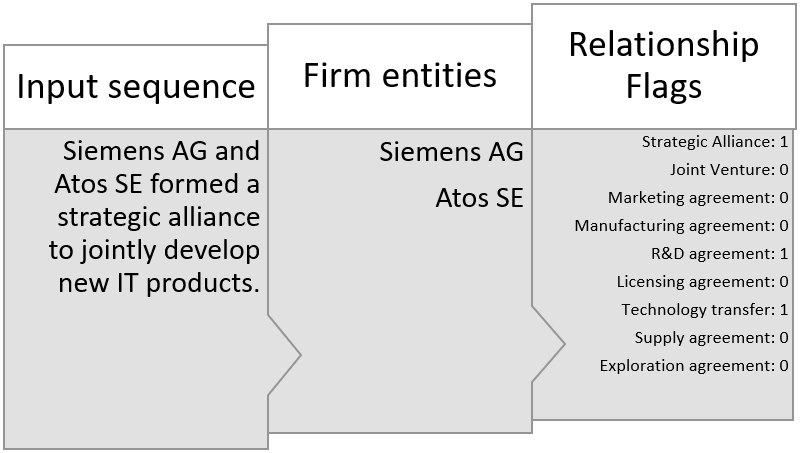
\includegraphics[width=0.55\textwidth]{./Figures/problem_statement.png} 
\caption{Joint entity and relationship extraction.} 
\label{fig:problem}
\end{figure}

%%%%%%%%%%%%%%%%%%%%%%%%%%%%%%%%%%%%%%%%%%%%%%%%%%%%%%%%%
\subsection{R\&D Collaborations from the LexisNexis News Database}
\label{sec:news}
%%%%%%%%%%%%%%%%%%%%%%%%%%%%%%%%%%%%%%%%%%%%%%%%%%%%%%%%%
We applied the text mining algorithm to articles from LexisNexis data lab, which provides millions of business news articles per day, going back to 1980. We select 1.5 million candidate articles by filtering articles on a list of keywords. In particular, to obtain articles that could contain alliance announcements, we applied a set of filters to LexisNexis' collection of news articles. We selected English language articles tagged as business news from news wires and press releases, newspapers, web-based publications, or industry trade press.  Additional information and details regarding the text mining algorithm and the news data can be found in Online Appendix \ref{sec:text-mining}. %Appendices \ref{sec:relationship_extraction_pipeline}, \ref{sec:knowledge_base} and \ref{sec:performance}.

Our resulting R\&D alliance database is much more comprehensive than other currently available databases. For R\&D collaborations, SDC Platinum, the de facto only comprehensive data set, contains only 14,832 such relations, while our data set contains around 52,445 and is less biased towards North American firms. %Time trends for the 5 most important industries and countries are plotted in Figures \ref{fig:top5-industries} and \ref{fig:top5-countries}, respectively. Figure \ref{fig:alliances_world_map} shows the locations (at the city level) and collaborations of the firms accumulated over all years (1980 to 2021). 
We complement the network data with information about firms' balance sheet information, locations, industries and patent activities. Online Appendix \ref{sec:app-data} provides further details including various descriptive statistics of the R\&D collaboration network. An illustration can be seen in Figure \ref{fig:2020_cc_graph}.

\begin{figure}[tbp]
%\begin{center}
%Year: 2020
%\end{center}
\vspace{-0.5cm}
\centering
\centerline{ \scalebox{0.75}{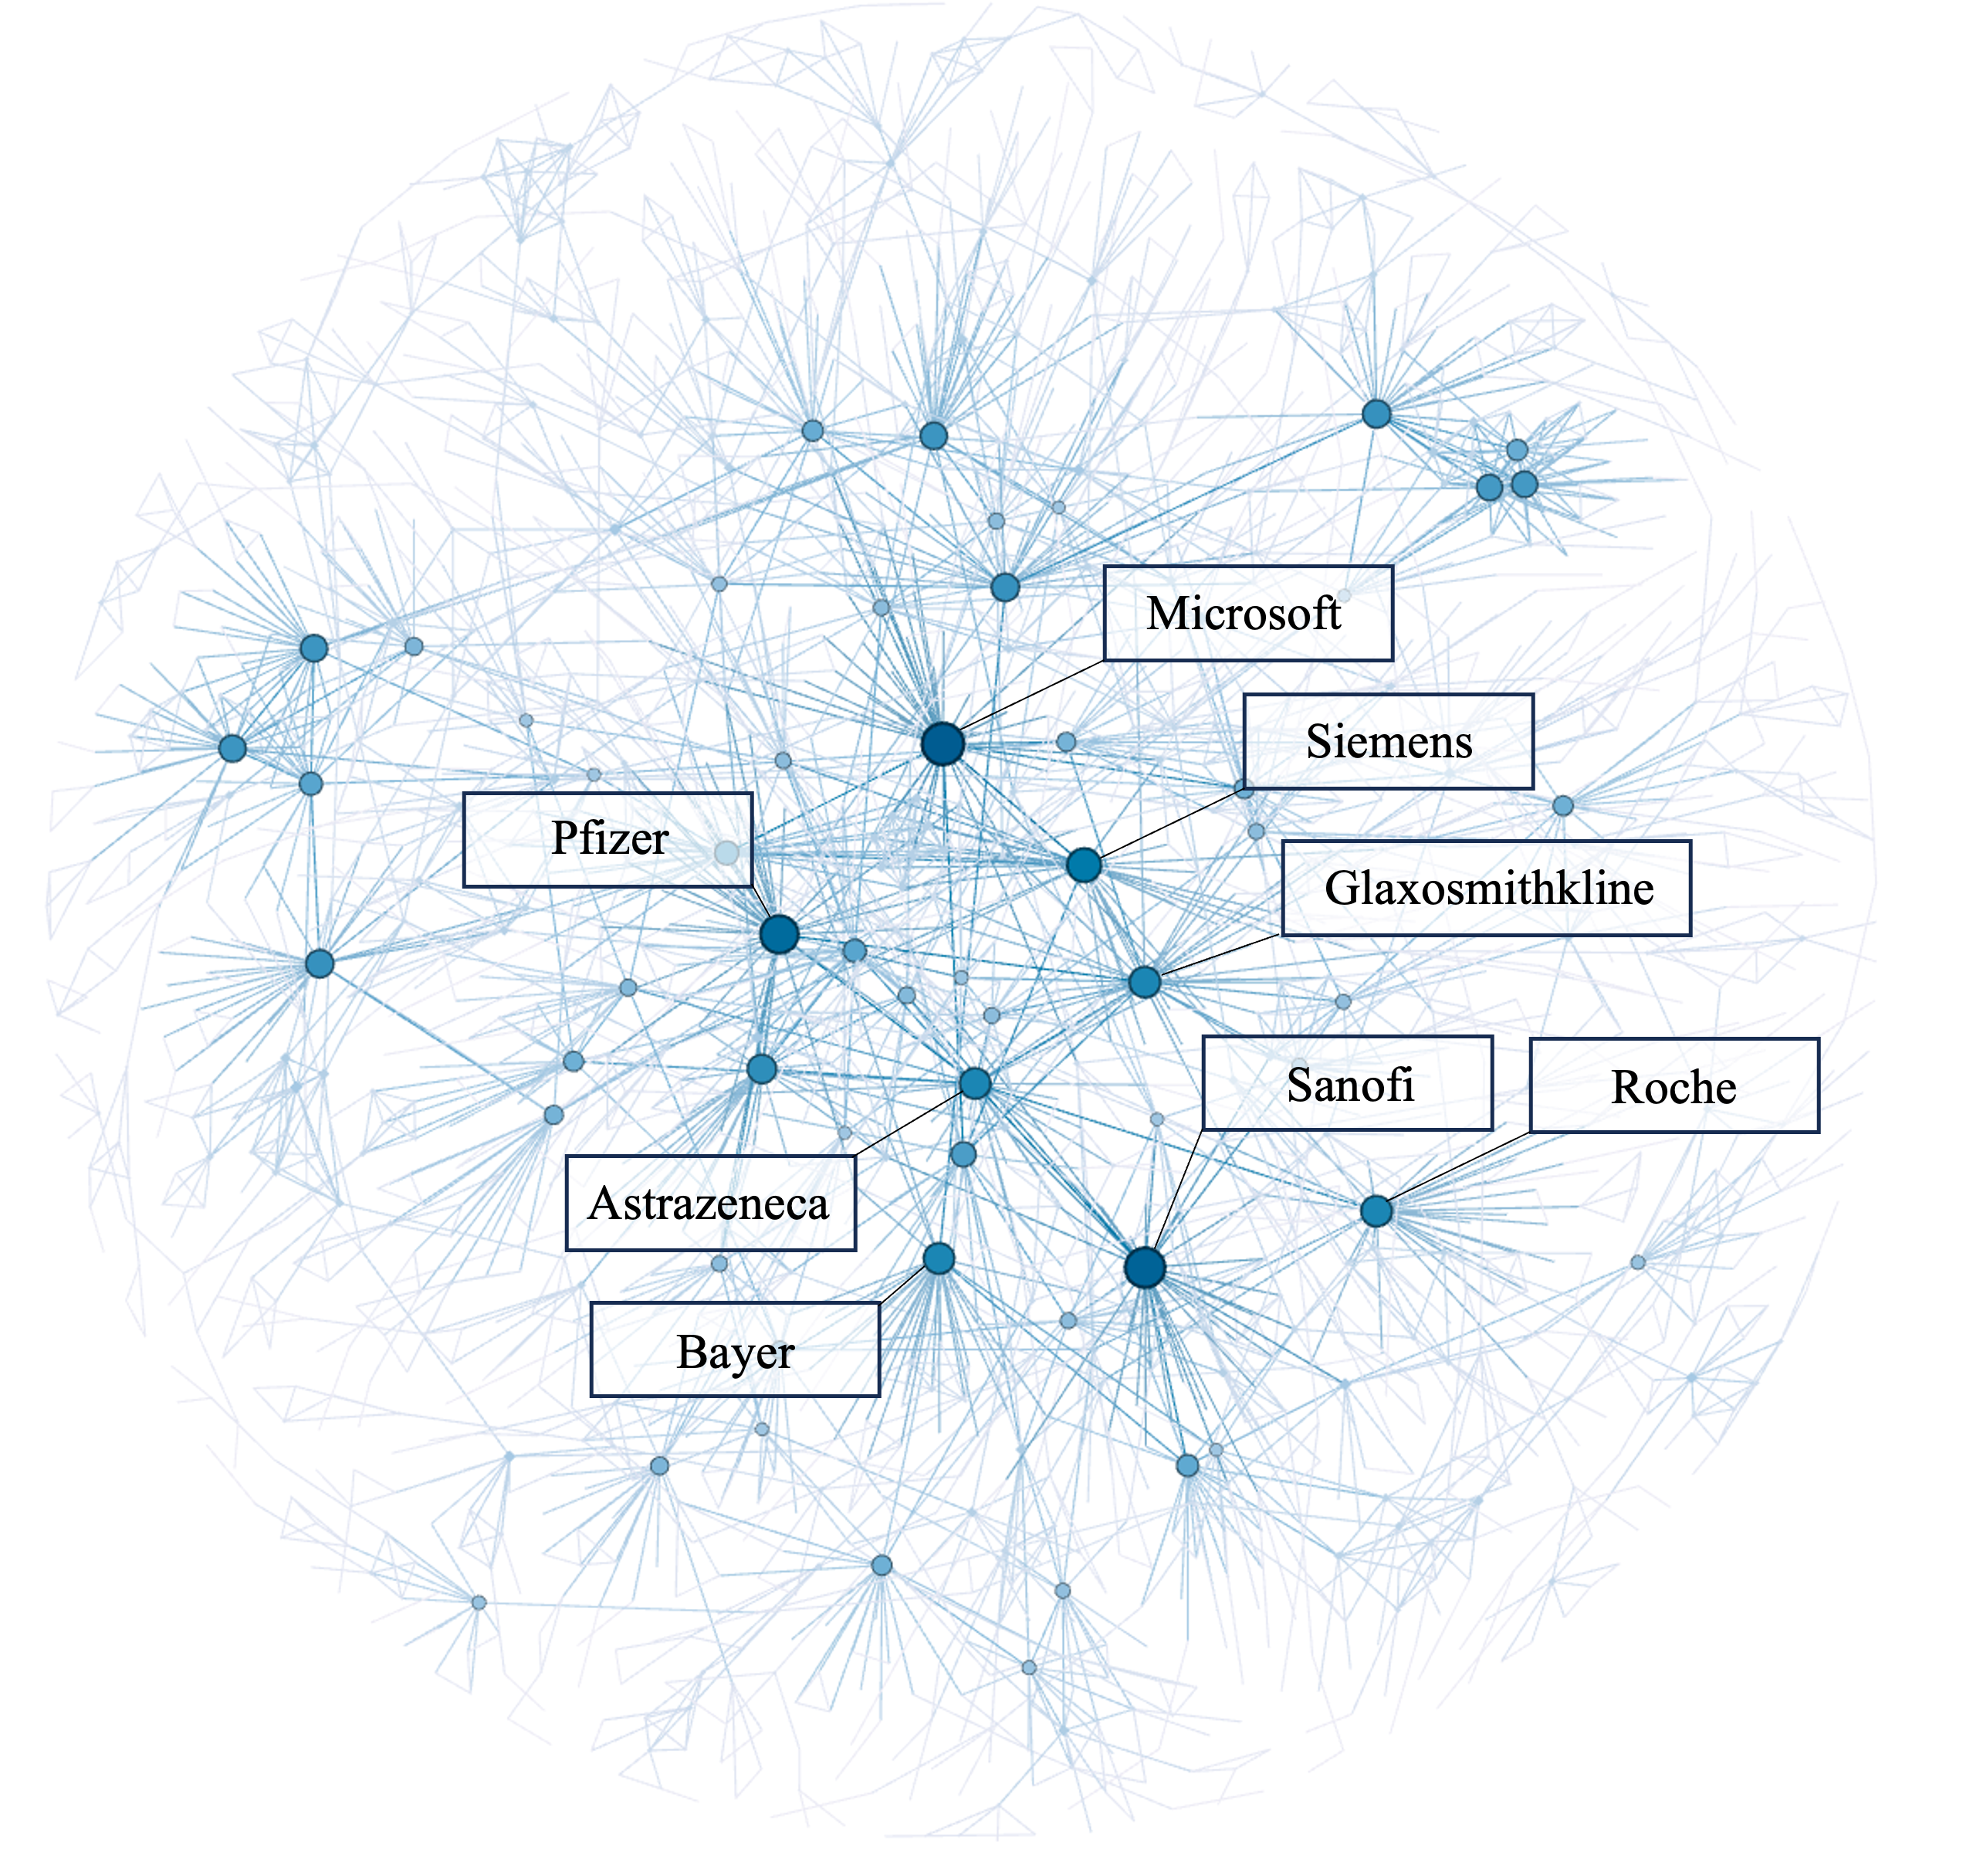
\includegraphics{./Figures/2020_cc_graph_5.png}}}
\caption{The largest connected component in the  network of R\&D
collaborations in the year 2020. The color of a node and its size scale with the number of R\&D collaborations, with the names of the $8$ largest firms mentioned
in the graph. The number of links is $3,307$, and the number of firms in the largest connected component is $1,826$.}
\label{fig:2020_cc_graph}
\end{figure}

%%%%%%%%%%%%%%%%%%%%%%%%%%%%%%%%%%%%%%%%%%%%%%%%%%%%%%%%%
\subsection{Text-Based Industry Classification and Accounting Data}
\label{sec:industry}
%%%%%%%%%%%%%%%%%%%%%%%%%%%%%%%%%%%%%%%%%%%%%%%%%%%%%%%%%
We identify the competition matrix $\mathbf{B}=(b_{ij,t})_{1 \le i,j \le n}$ using the matrix of Text-based Network Industry Classifications (TNIC) constructed by \citet{hoberg2016} from 10k filings of publicly listed firms.\footnote{See also: \url{https://hobergphillips.tuck.dartmouth.edu/}.} Since the bottom half of the TNIC pairwise similarity scores are small (less than 0.05), we define $b_{ij,t}=1$ if the corresponding TNIC similarity score is higher than the median, and $b_{ij,t}=0$ otherwise. Firms' sales and R\&D expenditures were obtained from the Compustat North America and Global Fundamentals databases as well as  Bureau van Dijk's Orbis database \citep{kalemli2024construct}. We compute a firm's output by dividing sales with the producer price index from the Bureau of Labor Statistics (at the NAICS 6-digit level where available and aggregated at the 4-digit level in the remaining cases). To measure a firm's productivity, we use the one-period lag of the firm's log R\&D capital stock. The R\&D capital stock is computed using a perpetual inventory method with 15\% depreciation rate \citep[][]{Bloom2013}.\footnote{Following the approach of \citet[][]{Hall2000} and \citet[][]{Bloom2013}, R\&D expenditures are used to compute R\&D capital stocks using the perpetual inventory method, with a depreciation rate of 15\%. %Specifically, the R\&D stock in year $t$ is given by $G_t = R_t +(1-\delta)G_{t-1}$, where $G_t$ is the R\&D stock in year $t$, $R_t$ is the R\&D flow expenditure in year $t$, and $\delta = 0.15$ represents the depreciation rate.
} 

%%%%%%%%%%%%%%%%%%%%%%%%%%%%%%%%%%%%%%%%%%%%%%%%%%%%%%%%%
\subsection{Sample Selection and Summary Statistics}
\label{sec:Sample_selection}
%%%%%%%%%%%%%%%%%%%%%%%%%%%%%%%%%%%%%%%%%%%%%%%%%%%%%%%%%
To study how technology spillovers change over time, we divide the years from 2001 to 2020 into four segments, each spanning five years. As a result, we will estimate the proposed model separately for four periods: 2001-2005, 2006-2010, 2011-2015, and 2016-2020. To construct the sample for estimation, we employ the following sample selection procedure: We begin with a total of 34,102 U.S. firms in the Compustat data. Then, for the samples in each period, we drop firms that contain missing values on either output or R\&D stock.\footnote{To mitigate the loss of firm observations due to missing values, we use linear interpolation to fill in missing values at certain years for the same firm.} Output has been computed using the Producer Price Index (PPI) of the US Bureau of Labor Statistics\footnote{See: \url{https://www.bls.gov/ppi/}.} matched to the year and NAICS code reported in the Compsutat sales item (in USD). Basic summary statistics can be found in Table~\ref{tab:summarystatistics_compustat}. The M\&A deals considered in our sample are summarized in Table \ref{tab:mna-data}.
       
\begin{center}
\singlespacing
\begin{threeparttable}[tp]
  \caption{Summary statistics.}
    \begin{tabular}{ccccccccccc}
    \toprule
          & \multicolumn{3}{c}{Output} & \multicolumn{3}{c}{Log R\&D Stock } & \multicolumn{3}{c}{Cost per Sale} & \multirow{ 2}{*}{\# of Firms} \\
    \cmidrule{2-4}\cmidrule{5-7}\cmidrule{8-10}  
          & Mean  & s.d.  & Max   & Mean  & s.d.  & Max   & Mean  & s.d. & Max   &  \\
    \midrule 
    2001-2005 & 6.56  & 36.28 & 934.08 & 2.31  & 2.36  & 9.85  & -0.30 & 1.15  & 8.63 & 1453 \\
    2006-2010 & 8.42  & 35.24 & 776.09 & 2.42  & 2.53  & 9.65  & -0.35 & 1.21  & 9.47 & 1332 \\
    2011-2015 & 11.12 & 44.90 & 999.73 & 2.56  & 2.66  & 9.44  & -0.40 & 1.18  & 9.23 & 1129 \\
    2016-2020 & 11.54 & 48.92 & 887.51 & 2.55  & 2.68  & 9.55  & -0.37 & 1.34  & 8.35 & 1143 \\
\midrule
    \bottomrule
    \end{tabular}
\begin{tablenotes}[flushleft]
\item \small \textbf{Notes:} Output is computed using the Producer Price Index (PPI) of the US Bureau of Labor Statistics matched to the year and the 6-digit level NAICS code reported in the Compsutat sales item (in USD), and is measured in millions. R\&D stock is measured in million USD.
\end{tablenotes}  
\label{tab:summarystatistics_compustat}%
\end{threeparttable}
\end{center}

\begin{center}
\singlespacing
\begin{threeparttable}[tp]
\caption{\label{tab:rnd-data} Number of R\&D collaborations.}
    \begin{tabular}{lccccc}    
    \toprule
    & Year 1 & Year 2 & Year 3 & Year 4 & Year 5  \\
    \midrule
    2001-2005 & 65    & 67    & 70     & 77  & 81 \\
    2006-2010 & 35    & 40    & 45     & 46  & 43 \\
    2011-2015 & 24    & 25    & 21     & 13  & 16 \\
    2016-2020 & 15    & 14    & 18     & 22  & 26 \\   
    \bottomrule  
    \end{tabular}%
  \label{tab:addlabel}%
\end{threeparttable}
\end{center}

\begin{center}
\singlespacing
\begin{threeparttable}[tp]
\caption{\label{tab:mna-data} Number of M\&A deals.}
    \begin{tabular}{lccccc}    
    \toprule
    & Year 1 & Year 2 & Year 3 & Year 4 & Year 5  \\
    \midrule
    2001-2005 & 31    & 14    & 17     & 15  & 20 \\
    2006-2010 & 24    & 28    & 24     & 15  & 21 \\
    2011-2015 & 20    & 17    & 15     & 13  & 17 \\
    2016-2020 & 19    & 12    & 12     & 11  & 12 \\     
    \bottomrule  
    \end{tabular}%
  \label{tab:addlabel}%
\end{threeparttable}
\end{center}

%%%%%%%%%%%%%%%%%%%%%%%%%%%%%%%%%%%%%%%%%%%%%%%%%%%%%%%%%
\section{Estimation Algorithm}
\label{sec:estimation-algorithm}
%%%%%%%%%%%%%%%%%%%%%%%%%%%%%%%%%%%%%%%%%%%%%%%%%%%%%%%%%
We apply a Bayesian MCMC approach for estimating the unknown parameter vector $\Theta=(\theta,\beta,\gamma,\kappa,\mu,\tau,\sigma^2_v)$. After dividing $\Theta$ into blocks, we adopt the Metropolis-Hastings-within-Gibbs sampling procedure to simulate draws with the conditional posterior distribution derived in Equation (\ref{eq:joint_likelihood_full}).

Note that the estimation algorithm requires repeatedly computing the matrix inverse $(\mathbf{I}_n + \lambda \mathbf{B} - \rho \mathbf{A})^{-1}$ in Equation (\ref{eq:bonacich}) after altering the network $G$ (and consequently its associated adjacency matrix $\mathbf{A}$), e.g., due to the formation or dissolution of an R\&D collaboration (adding or removing a link from the network) or a merger (swapping the links from the target node to the acquirer and removing the target from the network). Online Appendix \ref{sec:mat-perturb} provides a computationally efficient way to update the equilibrium output vector $\mathbf{y}$ after the addition or removal of a link in the network without recalculating the full matrix inverse.%\footnote{Online Appendix \ref{sec:br-part} provides a computationally efficient way to obtain an approximation to the Nash equilibrium output levels that is valid in sparse networks (as it is the case in the data).}

%%%%%%%%%%%%%%%%%%%%%%%%%%%%%%%%%%%%%%%%%%%%%%%%%%%%%%%%%
\section{Estimation Results}
\label{sec:results}
%%%%%%%%%%%%%%%%%%%%%%%%%%%%%%%%%%%%%%%%%%%%%%%%%%%%%%%%%
Based on our theoretical model derived in Section \ref{sec:dyn-rnd} we estimate the following equation:
\begin{equation}
y_{i,t}= \rho \sum_{j=1}^{n}a_{ij,t} y_{j,t} - \lambda \sum_{j=1}^{n}b_{ij,t} y_{j,t} + \beta x_{i,t-1} + \mu_i + \tau_t+ v_{i,t},
\end{equation}
where $\mathbf{y}_t = (y_{1,t},\ldots,y_{n,t})^\top$ denotes output~(measured in a million units), $\mathbf{x}_t=(x_{1t},\ldots,x_{nt})$ denotes the R\&D capital stock, $\mathbf{A}_t=(a_{ij,t})_{1 \le i,j \le n}$ is the adjacency matrix of R\&D collaborations, and $\mathbf{B}=(b_{ij,t})_{1 \le i,j \le n}$ is the competition matrix based on TNIC with granularity at the 3-digit SIC code level. 

%The estimation results for the R\&D network formation model outlined in Section \ref{sec:dyn-rnd} can be found in Table \ref{tab:result_output_US_compustat_NAICS_6_mna}. Model (1) corresponds to the estimation of Equation (\ref{eq:equilbrium_output}). Model (2) corresponds to the joint estimation of the output and R\&D collaboration decisions in Equation (\ref{eq:joint_likelihood}). We find that the spillover effect, $\rho$, is significant with the expected signs across all sample periods and specifications considered. Moreover, comparing the estimates for Models (1) and (2), there is an upward bias correction on the estimate of $\rho$ after controlling for network formation. This bias typically stems from unobserved firm-specific correlated effects that affect both the output of a firm and the R\&D collaborations it forms. Comparing the different sample periods we further find a cyclical pattern in the estimated spillover coefficient $\rho$. Moreover, product or market similarity (TNIC) tends to reduce the R\&D collaboration cost. Besides, past R\&D collaborations as well as having common R\&D collaboration partners in the past both reduce the cost of R\&D collaborations.

%\begin{table}[tbp]
% \small
%  \centering
%    \begin{center}
%    \begin{adjustbox}{max width=\textwidth,max totalheight=\textheight,keepaspectratio}
%\begin{threeparttable}
%\caption{\label{tab:result_output_US_compustat_NAICS_6} Estimation results for US publicly listed firms in the Compustat sample. {\red (This table is outdated) }  }
%    \begin{tabular}{llcccccccc}
%    \toprule
%          & & \multicolumn{2}{c}{2001-2005} & \multicolumn{2}{c}{2006-2010} & \multicolumn{2}{c}{2011-2015} & \multicolumn{2}{c}{2016-2020} \\
%          \cmidrule{3-10}
%          & & (1)  & (2) & (1)  & (2) & (1)  & (2) & (1)  & (2) \\
%    \midrule
%     \multicolumn{6}{l}{\bf Output} \\
%    \vspace{-0.25cm}\\
%   R\&D Spillover & ($\rho$)       & 0.3569   & 0.3120   & 0.1886   & 0.1841   & 0.3257   & 0.3168    & 0.2860    & 0.2799 \\
%   &              & (0.0064) & (0.0080) & (0.0058) & (0.0052) & (0.0107) & (0.0080)  & (0.0095)  & (0.0062) \\
%   Competition &  ($\lambda$)    & 0.0077   & 0.0083   & -0.0004  & -0.0005  & 0.0058   & 0.0059    & 0.0061    & 0.0060 \\
%     &              & (0.0018) & (0.0017) & (0.0018) & (0.0018) & (0.0030) & (0.0031)  &  (0.0031)  & (0.0030) \\
%   Productivity & ($\beta$)      & 2.7701   & 2.8332   & 4.2044   & 4.2204   & 5.3203   & 5.3357    & 5.7674    & 5.7893 \\
%    &              & (0.0997) & (0.0934) & (0.1121) & (0.1086) & (0.1523) & (0.1516)  & (0.2021)  & (0.1964) \\
%   Error Variance &  ($\sigma_v^2$) & 34.4858  & 31.3157  & 49.6113  & 49.5285  & 399.2705 & 397.7822  & 1108.2000 & 1109.0559 \\
%     &            & (0.8347) & (0.6235) & (1.1706) & (1.1626) & (22.3486)& (23.2114) & (30.1000) & (30.4574) \\   
%    \vspace{-0.25cm}\\
%\hdashline[0.4pt/2pt]
%\vspace{-0.25cm}\\
%    \multicolumn{6}{l}{\bf R\&D Collaboration Cost} \\   
%    \vspace{-0.25cm}\\
%    Constant & ($\gamma_0$)    &       & 6.1761    &       & 6.8030   &       & 6.7468   &       & 6.8541 \\
%    &              &       & (0.0970)  &       & (0.1541) &       & (0.2022) &       & (0.2233) \\
%    TNIC Similarity & ($\gamma_1$)    &       & -10.6231  &       & -10.9140 &       & -10.7475 &       & -8.3180 \\
%     &             &       & (1.1403)  &       & (1.0507) &       & (1.4031) &       & (1.3134) \\
%    Diff. Production & ($\gamma_2$)    &       & -0.0150   &       & -0.0256  &       & -0.0083  &       & -0.0097 \\
%     &             &       & (0.0019)  &       & (0.0048) &       & (0.0028) &       & (0.0019) \\
%    Diff. Production${}^{2}$ & ($\gamma_3$)    &       & 2.94E-05  &       & 9.38E-05 &       & 1.13E-05 &       & 9.79E-06 \\
%     &             &       & (7.00E-06)&       & (2.57E-05) &     & (6.41E-06) &     & (3.24E-06) \\
%    Past R\&D Collab. & ($\gamma_4$)    &       & -7.9829   &       & -13.4429 &       & -15.3902 &       & -14.1500 \\
%     &             &       & (0.1871)  &       & (1.7307) &       & (2.7478) &       & (2.4338) \\
%    R\&D Triangle Effect & ($\gamma_5$)    &       & -1.4348   &       & -2.3288  &       & -4.5298  &       & -2.2428 \\
%      &            &       &  (0.6488) &       & (0.6123) &       & (0.7163) &       & (1.1674) \\
%    % Scaling Factor & ($\delta$)      &       & -12.2093  &       & -9.7412  &       & -16.7175 &       & -13.4104 \\
%    %  &              &       & (0.1941)  &       & (0.1273) &       & (0.3867) &       & (0.4670) \\
%\midrule
%     \# of Firms &  ($n$)  & \multicolumn{2}{c}{1533} & \multicolumn{2}{c}{1394} & \multicolumn{2}{c}{1192} & \multicolumn{2}{c}{1215} \\
%\midrule
%    \bottomrule
%    \end{tabular}
%\begin{tablenotes}[flushleft]
%\item \small \textbf{Notes:} Model (1) corresponds to the estimation of Equation (\ref{eq:equilbrium_output}). Model (2) corresponds to the joint estimation of the output and R\&D collaboration decisions in Equation (\ref{eq:joint_likelihood}). Output is computed using NAICS 6-digit price indices from the BLS. The competition matrix $\textbf{B}$ is defined based on the TNIC data calibrated to be as granular as the three-digit SIC codes. The R\&D collaboration cost is specified as $\zeta_{ij,t}= 
%\phantom{\sum_k} \hspace{-0.5cm}
%\gamma_0
%+ \mathbf{c}_{ij,t} \gamma_1
%+
%\gamma_2 |y_{i,t-1}-y_{j,t-1}|
%+
%\gamma_3 |y_{i,t-1}-y_{j,t-1}|^2
%+
%\gamma_4 a_{ij,t-1}
%+
%\gamma_5 \sum_{k=1}^n a_{ik,t-1} a_{jk,t-1}.$
%\end{tablenotes}
%\end{threeparttable}
%    \end{adjustbox}
%\end{center}
%\end{table}

Table \ref{tab:result_output_US_compustat_NAICS_6_mna} presents the estimation results for the model outlined in Section \ref{sec:dyn-rnd-mna} where we control for both, the formation of R\&D collaborations and M\&As. Model (1) corresponds to the estimation Equation (\ref{eq:equilbrium_output}). Model (2) corresponds to the joint estimation of the output and R\&D collaboration decisions in Equation (\ref{eq:joint_likelihood_full}). For the estimates of the spillover coefficient, $\rho$, in Table \ref{tab:result_output_US_compustat_NAICS_6_mna}, we observe a cyclical pattern across the observation periods and some upward biases when failing to control for the endogeneity of R\&D collaborations and M\&As. Moreover, we find that market concentration (TNIC Similarity $\times$ TNIC HHI) leads to higher M\&A  costs, possibly due to barriers from antitrust policy regulations. Further, technological similarity, higher vertical relatedness, and a higher patent stock of the acquirer lead to lower M\&A costs. Notably, past R\&D collaborations significantly reduces the M\&A cost, and similarly, having more past common R\&D collaboration partners (R\&D triangle effect) decrease the M\&A cost. This supports the narrative of Section \ref{sec:model-implications} (cf. Eq. (\ref{eq:mna_rnd_cost-diff})) which identified R\&D collaborations as a stepping stone towards future M\&A integration. The significance and magnitudes of the cost-reducing effect of R\&D collaborations on M\&As, as well as the bias in the coefficients $\rho$ and $\lambda$ in Model (1), show the importance of jointly controlling for R\&D collaboration and M\&As in estimating technology spillover effects.
\begin{table}[tbp]
  \small
  \centering
    \begin{center}
        \begin{adjustbox}{max width=\textwidth,max totalheight=\textheight,keepaspectratio}
\begin{threeparttable}
\caption{\label{tab:result_output_US_compustat_NAICS_6_mna} Estimation results for US publicly listed firms in the Compustat sample.}
    \begin{tabular}{llcccccccc}
    \toprule
          & & \multicolumn{2}{c}{2001-2005} & \multicolumn{2}{c}{2006-2010} & \multicolumn{2}{c}{2011-2015} & \multicolumn{2}{c}{2016-2020} \\
          \cmidrule{3-10}
          & & (1)  & (2) & (1)  & (2) & (1)  & (2) & (1)  & (2) \\
    \midrule
    \multicolumn{6}{l}{\bf Output} \\
    \vspace{-0.25cm}\\
 R\&D Spillover  & ($\rho$)      & 0.3344   & 0.2998    & 0.1950   & 0.1863   & 0.3356   & 0.3142    & 0.2832    & 0.2758   \\
                    &               & (0.0053) & (0.0013)  & (0.0058) & (0.0023) & (0.0130) & (0.0014)  & (0.0097)  & (0.0035) \\
    Competition     & ($\lambda$)   & 0.0083   & 0.0081    & -0.0006  & -0.0008  & 0.0096   & 0.0084    & 0.005     & 0.0045   \\ 
                    &               & (0.0020) & (0.0015)  & (0.0018) & (0.0016) & (0.0034) & (0.0021)  & (0.0036)  & (0.0029) \\
    Log R\&D stock  & ($\beta_1$)   & 2.9838   & 3.0207    & 4.3529   & 4.3616   & 5.4424   & 5.4072    & 5.8651    & 5.8591   \\
                    &               & (0.1075) & (0.1194)  & (0.1103) & (0.0971) & (0.1637) & (0.1940)  & (0.2083)  & (0.1659) \\
    Log cost ratio  & ($\beta_2$)   & -0.2198  & -0.1997   & -0.2292  & -0.2559  & -0.7760  & -0.8619   & -1.0167   & -1.1289  \\
                    &               & (0.1149) & (0.1089)  & (0.1433) & (0.1215) & (0.3274) & (0.2656)  & (0.4017)  & (0.2525) \\
    Error Variance & ($\sigma_v^2$) & 32.9052  & 30.5319   & 52.7175  & 52.7423  & 510.9221 & 509.4280  & 1245.7000 & 1247.9125 \\
                    &               & (0.8090) & (0.6308)  & (1.3287) & (1.2609) & (23.9044)& (23.5688) & (33.1000) & (34.0170) \\
        \vspace{-0.25cm}\\
\hdashline[0.4pt/2pt]
\vspace{-0.25cm}\\
    \multicolumn{6}{l}{\bf R\&D Collaboration Cost} \\
    \vspace{-0.25cm}\\
Constant                 & ($\gamma_0$)  &  &        6.0700            &  & 6.6629   &  &          6.6319   &  &        6.6824   \\
                             &               &  &       (0.0708) &  &           (0.1509) &  &          (0.1942) &  &        (0.2043) \\
    TNIC Similarity          & ($\gamma_1$)  &  &        -5.9933  &  &           -6.6903  &  &          -4.3878  &  &        -5.3433  \\
                             &               &  &        (0.2886) &  &           (0.7959) &  &          (0.7634) &  &        (1.1814) \\
    TNIC Vertical Relatedness     & ($\gamma_2$)  &  &        -8.6669  &  &           -8.9939  &  &          -11.6004 &  &        -9.8753  \\
                             &               &  &        (1.3227) &  &           (1.9552) &  &          (4.2037) &  &        (4.5018) \\
    Patent Tech Similarity   & ($\gamma_3$)  &  &        -7.4095  &  &           -7.0657  &  &          -7.1227  &  &        -15.7681 \\
                             &               &  &       (0.1415) &  &           (0.1636) &  &          (0.2932) &  &        (2.0659) \\ 
    Diff. Production         & ($\gamma_4$)  &  &        -0.0138  &  &           -0.0183  &  &          0.0020   &  &        -0.0082  \\
                             &               &  &        (0.0018) &  &           (0.0033) &  &          (0.0035) &  &        (0.0016) \\
    Diff. Production${}^{2}$ & ($\gamma_5$)  & &        3.05e-5  & &           5.49e-5  &  &        -2.68e-6 &   &     9.16e-6   \\
                             &               &  &      (8.75e-6)&     &      (1.38e-5)&     &     (6.46e-6)&   &     (3.05e-6) \\
    Past R\&D Collab.        & ($\gamma_6$)  &  &      -0.3136  &   &        -2.5327  &   &       -3.0999  &   &     -1.6632  \\
                             &               &  &      (0.2479) &  &         (0.4974) &  &        (0.7892) & &       (0.9669) \\
    R\&D Triangle Effect     & ($\gamma_7$)  &   &     -1.5333  &    &       -1.9032  &    &      -1.7946  &  &      -1.6098  \\
                             &               &  &      (0.1823) &   &        (0.2060) &      &    (0.2875) &     &   (0.2742) \\ 
\vspace{-0.25cm}\\
\hdashline[0.4pt/2pt]
\vspace{-0.25cm}\\
    \multicolumn{6}{l}{\bf M\&A Cost} \\
    \vspace{-0.25cm}\\
Constant                 & ($\kappa_0$)  &  &     12.3712  &  &     12.7767  & &       13.4370  &  &      13.8160  \\ 
                             &               &    &   (0.1886) & &      (0.1993) & &       (0.2927) &   &     (0.3195) \\
    TNIC Similarity          & ($\kappa_1$)  &   &    1.7960   &  &     1.4459   &     &   0.0881   &     &   1.9493   \\
                             &               &    &   (0.4222) &     &  (1.2950) &    &   (1.3753) &       & (1.6964) \\
    TNIC Similarity $\times$ TNIC HHI & ($\kappa_2$) &    &  1.0875   &    &   2.2304   &    &    4.7950   &    &    4.9632   \\
                             &               &    &   (0.5975) &  &     (0.7429) &     &   (0.8863) &     &   (2.8031) \\
    TNIC Vertical Relatedness     & ($\kappa_3$)  &  &     -1.7120  &  &     -3.2584  &    &    -2.0389  &      &  -3.7848  \\
                             &               &    &   (0.8887) &   &    (1.4800) &     &   (0.2910) &     &   (2.1744) \\
    Patent Tech Similarity   & ($\kappa_4$)  &    &   -4.1065  &     &  -3.8706  &      &  -4.2306  &    &    -4.2618  \\
                             &               &     &  (0.2794) &   &    (0.2795) &  &      (0.2985) &    &    (0.2971)  \\
    Patent Stock~(Acquirer)  & ($\kappa_5$)  &    &   -0.1604  &    &   -0.3448  &   &     -0.2655  &    &    -0.3067   \\
                             &               &    &   (0.0476) &  &     (0.0501) &   &     (0.0737) &      &  (0.0856)  \\
    Patent Stock~(Target)    & ($\kappa_6$)  &   &    0.0766   &   &    0.0910   &   &     -0.1227  &    &    -0.2104   \\
                             &               &    &   (0.0601) &    &   (0.0513) &      &  (0.0629) &     &   (0.0779)  \\
    Diff. Production         & ($\kappa_7$)  &    &   -0.0134  &   &    -0.0254  &   &     -0.0490  &     &   -0.0434   \\
                             &               &   &    (0.0034) &    &   (0.0060) &   &     (0.0116) &      &  (0.0105)  \\
    Diff. Production${}^{2}$ & ($\kappa_8$)  &     &   2.53e-5 &    &    1.40e-5 &     &    3.82e-4 &     &    3.11e-4    \\
                             &               &   &    (1.00e-5)&     &  (3.61e-5)& &       (1.01e-4)&   &     (1.01e-4)  \\
    Past R\&D Collab.        & ($\kappa_9$)  &     &  -3.8038  &   &    -2.7467  &   &     -2.2055  &     &   -9.7494   \\
                             &               &   &    (0.2590) &   &    (0.4754) &   &     (0.9534) &    &    (1.0926)  \\
    R\&D Triangle Effect     & ($\kappa_{10}$) &     &  -2.1274  &  &     -3.2707  &   &     -2.4508  &    &    -1.9453   \\
                             &               &    &   (0.3874)    &    &(0.8247) &   &     (0.8618) &     &   (1.2058)  \\ 
\midrule
    \# of Firms &  ($n$)     & \multicolumn{2}{c}{1453} & \multicolumn{2}{c}{1332} & \multicolumn{2}{c}{1129} & \multicolumn{2}{c}{1143} \\
\midrule
    \bottomrule
    \end{tabular}
\begin{tablenotes}[flushleft]
\item \small \textbf{Notes:} Model (1) corresponds to the estimation  Equation (\ref{eq:equilbrium_output}). Model (2) corresponds to the joint estimation of the output and R\&D collaboration decisions in Equation (\ref{eq:joint_likelihood_full}). Output is computed using NAICS 6-digit price indices from the BLS. The competition matrix $\textbf{B}$ is defined based on the TNIC data calibrated to be as granular as the three-digit SIC codes. The R\&D collaboration cost is specified as $\zeta_{ij,t}=
\phantom{\sum_k} \hspace{-0.5cm}
\gamma_0
+ \mathbf{c}_{ij,t} \gamma_1
+
\mathbf{p}_{ij,t}\gamma_2
+
\mathbf{v}_{ij,t}\gamma_3
+
\mathbf{d}_{ij,t}\gamma_4 
+
\gamma_5 a_{ij,t-1}
+
\gamma_6 \sum_{k=1}^n a_{ik,t-1} a_{jk,t-1}
+
\gamma_7 |y_{i,t-1}-y_{j,t-1}|
+
\gamma_8 |y_{i,t-1}-y_{j,t-1}|^2.$
The M\&A cost is specified as $\nu_{ij,t}
=
\phantom{\sum_k} \hspace{-0.5cm}
\kappa_0
+
\mathbf{c}_{ij,t} \kappa_1
+
\mathbf{c}_{ij,t}{\rm HHI}_{i,t} \kappa_2
+
\mathbf{p}_{ij,t}\kappa_3
+
\mathbf{v}_{ij,t}\kappa_4
+
\mathbf{d}_{ij,t}\kappa_5
+
\mathbf{s}_{i,t} \kappa_6
+
\mathbf{s}_{j,t} \kappa_7
+
\kappa_{8} a_{ij,t-1}
+
\kappa_{9} \sum_{k=1}^n a_{ik,t-1} a_{jk,t-1}
+
\kappa_{10} (y_{i,t-1}-y_{j,t-1})
+
\kappa_{11} (y_{i,t-1}-y_{j,t-1})^2.$
\end{tablenotes}
\end{threeparttable}
    \end{adjustbox}
\end{center}
\end{table}

% \begin{table}[tbp]
%   \small
%   \centering
%     \begin{center}
%         \begin{adjustbox}{max width=\textwidth,max totalheight=\textheight,keepaspectratio}
% \begin{threeparttable}
% \caption{\label{tab:result_output_US_compustat_NAICS_6_mna} Estimation results for US publicly listed firms in the Compustat sample.}
%     \begin{tabular}{llcccccccc}
%     \toprule
%           & & \multicolumn{2}{c}{2001-2005} & \multicolumn{2}{c}{2006-2010} & \multicolumn{2}{c}{2011-2015} & \multicolumn{2}{c}{2016-2020} \\
%           \cmidrule{3-10}
%           & & (1)  & (2) & (1)  & (2) & (1)  & (2) & (1)  & (2) \\
%     \midrule
%     \multicolumn{6}{l}{\bf Output} \\
%     \vspace{-0.25cm}\\
%     R\&D Spillover  & ($\rho$)      & 0.2993   & 0.2893    & 0.1950   & 0.1911   & 0.3338   & 0.3242    & 0.2833    & 0.2745   \\
%                     &               & (0.0018) & (0.0017)  & (0.0058) & (0.0061) & (0.0100) & (0.0078)  & (0.0093)  & (0.0099) \\
%     Competition     & ($\lambda$)   & 0.0089   & 0.0088    & -0.0006  & -0.0004  & 0.0098   & 0.0096    & 0.0053    & 0.0039   \\ 
%                     &               & (0.0018) & (0.0018)  & (0.0018) & (0.0017) & (0.0035) & (0.0033)  & (0.0034)  & (0.0013) \\
%     Log R\&D stock  & ($\beta_1$)   & 3.0857   & 3.0792    & 4.3529   & 4.3502   & 5.4385   & 5.4328    & 5.8748    & 5.8411   \\
%                     &               & (0.1073) & (0.1053)  & (0.1103) & (0.1121) & (0.1629) & (0.1610)  & (0.2075)  & (0.2053) \\
%     Log cost ratio  & ($\beta_2$)   & -0.1994  & -0.1964   & -0.2292  & -0.2230  & -0.7795  & -0.7780   & -1.0355   & -1.0387  \\
%                     &               & (0.1114) & (0.1107)  & (0.1433) & (0.1421) & (0.3306) & (0.3258)  & (0.4038)  & (0.4000) \\
%     Error Variance & ($\sigma_v^2$) & 30.5161  & 30.5180   & 52.7175  & 52.9210  & 513.7557 & 513.2189  & 1247.0000 & 1248.5000 \\
%                     &               & (0.6458) & (0.6421)  & (1.3287) & (1.2930) & (24.2116)& (23.5051) & (34.1000) & (33.7000) \\
%         \vspace{-0.25cm}\\
% \hdashline[0.4pt/2pt]
% \vspace{-0.25cm}\\
%     \multicolumn{6}{l}{\bf R\&D Collaboration Cost} \\
%     \vspace{-0.25cm}\\
% Constant                  & ($\gamma_0$)   &  & 6.3498    &           & 7.1763    &           & 7.2800    &       & 6.9424 \\    
%                           &                &  & (0.0977)  &           & (0.2576)  &           & (0.3179)  &       & (0.1871) \\  
% TNIC Similarity           & ($\gamma_1$)   &  & -5.6160   &           & -8.8227   &           & -5.6590   &       & -5.4382 \\   
%                           &                &  & (0.5601)  &           & (1.1424)  &           & (0.9819)  &       & (1.2406) \\  
% Vertical Relatedness      & ($\gamma_2$)   &  & -10.4084  &           & -28.5234  &           & -9.2044   &       & -8.8420 \\   
%                           &                &  & (6.5636)  &           & (3.9547)  &           & (2.9543)  &       & (1.4322) \\  
% Patent Tech Similarity    & ($\gamma_3$)   &  & -1.9752   &           &  -2.4504  &           & -1.3543   &       & -1.6633 \\   
%                           &                &  & (0.1921)  &           & (0.3347)  &           & (0.5530)  &       & (0.3174) \\  
% Diff. Production          & ($\gamma_4$)   &  & -0.0143   &           & -0.0257   &           & -0.0272   &       & -0.0095 \\   
%                           &                &  & (0.0021)  &           & (0.0058)  &           & (0.0097)  &       & (0.0018) \\  
% Diff. Production${}^{2}$  & ($\gamma_5$)   &  & 2.82E-05  &           & 9.83E-05  &           & 1.11E-04  &       & 1.05E-05 \\  
%                           &                &  &(8.52E-06) &           &(2.99E-05) &           &(5.26E-05) &       &(3.52E-06)\\  
% Past R\&D Collab.         & ($\gamma_6$)   &  & -7.4064   &           & -7.1245   &           & -21.3128  &       & -22.4870 \\  
%                           &                &  & (0.2568)  &           & (0.3347)  &           & (1.0029)  &       & (0.6165) \\  
% R\&D Triangle Effect      & ($\gamma_7$)   &  & 0.8761    &           & -4.1772   &           & 0.2223    &       & -14.7044 \\  
%                           &                &  & (0.4670)  &           & (0.5125)  &           & (0.5238)  &       & (2.0567) \\  
%                                  \vspace{-0.25cm}\\
% \hdashline[0.4pt/2pt]
% \vspace{-0.25cm}\\
%     \multicolumn{6}{l}{\bf M\&A Cost} \\
%     \vspace{-0.25cm}\\
%     Constant                    & ($\kappa_0$)   &    & 12.4999 &       & 12.5312 &       & 13.1444 &       & 14.0927 \\        
%                                 &                &    & (0.2310) &       & (0.1997) &       & (0.2068) &       & (0.0685) \\    
%     TNIC Similarity             & ($\kappa_1$)   &    & -7.2195 &       & -12.1910 &       & -11.1752 &       & -7.9324 \\      
%                                 &                &    & (1.0250) &       & (0.9397) &       & (0.3670) &       & (0.3271) \\    
%     TNIC Similarity*TNIC HHI    &  ($\kappa_2$)  &    & 12.9779 &       & 19.3016 &       & 12.5339 &       & 10.7897 \\        
%                                 &                &    & (0.6565) &       & (0.2781) &       & (0.3851) &       & (0.0868) \\    
%     vertical relatedness        & ($\kappa_3$)   &    & -9.9782 &       & -6.2604 &       & -6.7211 &       & -7.8529 \\        
%                                 &                &    & (0.8677) &       & (1.1745) &       & (0.1025) &       & (0.1636) \\    
%     Patent Tech Similarity      & ($\kappa_4$)   &    & -3.7101 &       & -3.0660 &       & -3.7269 &       & -3.6400 \\        
%                                 &                &    & (0.3133) &       & (0.2957) &       & (0.0920) &       & (0.1770) \\    
%     Patent Stock -- Acquirer    & ($\kappa_5$)   &    & -0.1912 &       & -0.2958 &       & -0.1651 &       & -0.3549 \\        
%                                 &                &    & (0.0652) &       & (0.0541) &       & (0.0652) &       & (0.0725) \\    
%     Patent Stock -- Target      & ($\kappa_6$)   &    & 0.0797 &       & 0.1018 &       & -0.1089 &       & -0.2391 \\          
%                                 &                &    & (0.0664) &       & (0.0564) &       & (0.0475) &       & (0.0467) \\    
%     Diff. Production            & ($\kappa_7$)   &    & -0.0131 &       & -0.0250 &       & -0.0619 &       & -0.0432 \\        
%                                 &                &    & (0.0046) &       & (0.0071) &       & (0.0095) &       & (0.0086) \\    
%     Diff. Production Square     & ($\kappa_8$)   &    & 2.53E-05 &       & 1.26E-04 &       & 4.56E-04 &       & 2.93E-04 \\    
%                                 &                &    &(1.31E-05) &       &(4.28E-05) &      &(9.25E-05) &       &(7.44E-05) \\ 
%     Past R\&D Collaboration     & ($\kappa_9$)   &    & -2.5831 &       & -4.4666 &       & -7.6501 &       & -1.4406 \\        
%                                 &                &    & (0.3063) &       & (0.5475) &       & (0.2543) &       & (0.2965) \\    
%     R\&D Triangle Effect        & ($\kappa_{10}$)  &    & -0.4449 &       & 16.4429 &       & 3.9830 &       & 4.3191 \\          
%                                 &                &    & (0.7490) &       & (1.0315) &       & (0.1466) &       & (0.2453) \\    
%     % Scaling Factor           & ($\delta$)    &       & -18.7076 &       & -11.7912 &       & -13.4278 &       & -16.0926 \\
%     %                          &               &       & (0.2649) &       & (0.8819) &       & (0.4261) &       & (0.5697) \\
% \midrule
%     \# of Firms &  ($n$)     & \multicolumn{2}{c}{1453} & \multicolumn{2}{c}{1332} & \multicolumn{2}{c}{1129} & \multicolumn{2}{c}{1143} \\
% \midrule
%     \bottomrule
%     \end{tabular}
% \begin{tablenotes}[flushleft]
% \item \small \textbf{Notes:} Model  (1) corresponds to the estimation  Equation (\ref{eq:equilbrium_output}). Model  (2) corresponds to the joint estimation of the output and R\&D collaboration decisions in Equation (\ref{eq:joint_likelihood_full}). Output is computed using NAICS 6-digit price indices from the BLS. The competition matrix $\textbf{B}$ is defined based on the TNIC data calibrated to be as granular as the three-digit SIC codes.
% The R\&D collaboration cost is specified as $\zeta_{ij,t}=
% \phantom{\sum_k} \hspace{-0.5cm}
% \gamma_0
% + \mathbf{c}_{ij,t} \gamma_1
% +
% \mathbf{v}_{ij,t}\gamma_2
% +
% \mathbf{p}_{ij,t}\gamma_3
% +
% \gamma_4 |y_{i,t-1}-y_{j,t-1}|
% +
% \gamma_5 |y_{i,t-1}-y_{j,t-1}|^2
% +
% \gamma_6 a_{ij,t-1}
% +
% \gamma_7 \sum_{k=1}^n a_{ik,t-1} a_{jk,t-1}.$
% The M\&A cost is specified as $\nu_{ij,t}
% =
% \phantom{\sum_k} \hspace{-0.5cm}
% \kappa_0
% +
% \mathbf{c}_{ij,t} \kappa_1
% +
% \mathbf{c}_{ij,t}*{\rm HHI}_{i,t} \kappa_2
% +
% \mathbf{v}_{ij,t}\kappa_3
% +
% \mathbf{p}_{ij,t}\kappa_4
% +
% \mathbf{s}_{i,t} \kappa_5
% +
% \mathbf{s}_{j,t} \kappa_6
% +
% \kappa_7 (y_{i,t-1}-y_{j,t-1})
% +
% \kappa_8 (y_{i,t-1}-y_{j,t-1})^2
% +
% \kappa_{9} a_{ij,t-1}
% +
% \kappa_{10} \sum_{k=1}^n a_{ik,t-1} a_{jk,t-1}.$
% \end{tablenotes}
% \end{threeparttable}
%     \end{adjustbox}
% \end{center}
% \end{table}

% \begin{table}[tbp]
%   \small
%   \centering
%     \begin{center}
%         \begin{adjustbox}{max width=\textwidth,max totalheight=\textheight,keepaspectratio}
% \begin{threeparttable}
% \caption{Marginal Effects on R\&D Collaboration and M\&A }
% \begin{tabular}{llcccc}
% \hline
%  &  & 2001--2005 & 2006--2010 & 2011--2015 & 2016--2020 \\
% Variable & $\Delta X$ (unit) & $\Delta$ Prob (\%) & $\Delta$ Prob (\%) & $\Delta$ Prob (\%) & $\Delta$ Prob (\%) \\
% \hline

% \multicolumn{6}{l}{\textbf{R\&D Collaboration}} \\

% TNIC Similarity 
% & one s.d. 
% & 3.52E-04 & 3.19E-04 & 3.76E-05 & 0.0001 \\
% & 
% & (0.0180) & (0.0228) & (0.0009) & (0.0040) \\

% Past R\&D Collaboration 
% & 0 to 1 
% & 59.7690 & 32.8000 & 99.9950 & 99.9966 \\
% & 
% & (7.8377) & (13.5280) & (0.6873) & (0.5331) \\

% R\&D Triangle Effect 
% & increase by one 
% & -2.93E-03 & 0.8761 & -0.0001 & 99.9256 \\
% & 
% & (0.2102) & (2.6094) & (0.0030) & (0.5493) \\

% Patent Tech Similarity 
% & one s.d. 
% & 0.0009 & 0.0007 & 0.0001 & 0.0003 \\
% & 
% & (0.0415) & (0.0419) & (0.0003) & (0.0066) \\

% Vertical Relatedness 
% & one s.d. 
% & 1.40E-04 & 0.0002 & 1.09E-05 & 2.69E-05 \\
% & 
% & (0.0073) & (0.0149) & (0.0000) & (0.0005) \\

% Diff.\ Production 
% & increase by 50\% 
% & 0.0004 & 0.0001 & 4.69E-05 & 8.64E-05 \\
% & 
% & (0.0252) & (0.0779) & (0.0015) & (0.0023) \\

% \multicolumn{6}{l}{\textbf{M\&A }} \\

% TNIC Similarity 
% & one s.d. 
% & 5.43E-05 & 0.0001 & 0.0002 & 1.21E-04 \\
% & 
% & (0.0002) & (0.0006) & (0.0018) & (0.0014) \\

% TNIC HHI 
% & one s.d. 
% & -4.73E-05 & -6.93E-05 & -0.0001 & -8.60E-05 \\
% & 
% & (0.0032) & (0.0060) & (0.0111) & (0.0058) \\

% Past R\&D Collaboration 
% & 0 to 1 
% & 0.0009 & 0.0284 & -0.0027 & -0.0008 \\
% & 
% & (0.0027) & (0.0281) & (0.0406) & (0.0084) \\

% R\&D Triangle Effect 
% & increase by one 
% & 0.0005 & -0.0011 & -0.0011 & -0.0008 \\
% & 
% & (0.0039) & (0.0039) & (0.0132) & (0.0073) \\

% Patent Tech Similarity 
% & one s.d. 
% & 0.0004 & 0.0005 & 0.0008 & 0.0006 \\
% & 
% & (0.0015) & (0.0015) & (0.0119) & (0.0054) \\

% Vertical Relatedness 
% & one s.d. 
% & 2.78E-05 & 2.13E-05 & 2.43E-05 & 2.14E-05 \\
% & 
% & (0.0001) & (0.0001) & (0.0004) & (0.0002) \\

% Patent Stock -- Acquiror 
% & increase by 50\% 
% & 0.0003 & 0.0010 & 0.0005 & 0.0011 \\
% & 
% & (0.0028) & (0.0080) & (0.0081) & (0.0222) \\

% Patent Stock -- Target 
% & increase by 50\% 
% & -0.0001 & -0.0001 & 0.0002 & 0.0003 \\
% & 
% & (0.0005) & (0.0006) & (0.0036) & (0.0063) \\

% Diff.\ Production 
% & increase by 50\% 
% & 3.83E-05 & 1.06E-05 & 4.98E-05 & 6.33E-06 \\
% & 
% & (0.0005) & (0.0012) & (0.0046) & (0.0038) \\

% \hline
% \end{tabular}
% \end{threeparttable}
%     \end{adjustbox}
% \end{center}
% \end{table}

%\begin{table}[tbp]
%  \small
%  \centering
%    \begin{center}
%        \begin{adjustbox}{max width=\textwidth,max totalheight=\textheight,keepaspectratio}
%\begin{threeparttable}
%\caption{\label{tab:result_output_international_compustat_NAICS_6_mna} Estimation results for international publicly listed firms in the Compustat sample.}
%    \begin{tabular}{llcccc}
%    \toprule
%          & & \multicolumn{1}{c}{2001-2005} & \multicolumn{1}{c}{2006-2010} & \multicolumn{1}{c}{2011-2015} & \multicolumn{1}{c}{2016-2020} \\
%    \midrule
%    \multicolumn{6}{l}{\bf Output} \\
%    \vspace{-0.25cm}\\
%    R\&D Spillover  & ($\rho$)      &   &  &   & 0.0683        \\
%                    &               &   &  &   & (0.0025)     \\
%    Competition     & ($\lambda$)   &   &  &   & 5.18e-5      \\ 
%                    &               &   &  &   & (2.8e-5)    \\
%    Log R\&D stock  & ($\beta_1$)   &   &  &   & 3.6996       \\
%                    &               &   &  &   & (0.0559)     \\
%    Log labor prod. & ($\beta_2$)   &   &  &   & 3.7104       \\
%                    &               &   &  &   & (0.1594)    \\
%    Error Variance & ($\sigma_v^2$) &   &  &   & 54.5289      \\
%                    &               &   &  &   & (1.0698)    \\
%\midrule
%    \# of Firms &  ($n$)     & \multicolumn{1}{c}{ } & \multicolumn{1}{c}{ } & \multicolumn{1}{c}{ } & \multicolumn{1}{c}{3643} \\
%\midrule
%    \bottomrule
%    \end{tabular}
%\begin{tablenotes}[flushleft]
%\item \small \textbf{Notes:} Output is computed using NAICS 6-digit price indices from the BLS. The competition matrix $\textbf{B}$ is constructed based on the company website product descriptions.
%\end{tablenotes}
%\end{threeparttable}
%    \end{adjustbox}
%\end{center}
%\end{table}

\FloatBarrier

%%%%%%%%%%%%%%%%%%%%%%%%%%%%%%%%%%%%%%%%%%%%%%%%%%%%%%%%%
\section{Counterfactuals}
\label{sec:counterfactual}
%%%%%%%%%%%%%%%%%%%%%%%%%%%%%%%%%%%%%%%%%%%%%%%%%%%%%%%%%
We use the structural estimates reported in Table \ref{tab:result_output_US_compustat_NAICS_6_mna} to evaluate the role of organizational choice in innovation through a set of counterfactual simulations. The key objective is to quantify how aggregate output responds to restrictions on alternative governance modes for internalizing technological complementarities.

%%%%%%%%%%%%%%%%%%%%%%%%%%%%%%%%%%%%%%%%%%%%%%%%%%%%%%%%%
\subsection{Counterfactual Design}
%%%%%%%%%%%%%%%%%%%%%%%%%%%%%%%%%%%%%%%%%%%%%%%%%%%%%%%%%
We consider three counterfactual scenarios:
\begin{enumerate}
    \item \textbf{No M\&A:} all merger and acquisition (M\&A) links are removed;
    \item \textbf{No alliances:} all R\&D collaboration links are removed;
    \item \textbf{No M\&A and no alliances:} both governance margins are shut down.
\end{enumerate}
In the first scenario, we undo all observed M\&A deals and restore merged firms to their pre-merger identities.\footnote{The accounting decomposition undoes the observed deals mechanically,
splitting each merged entity into its pre-transaction constituents and
recomputing outputs from Equation~(\ref{eq:bonacich}) along the observed
collaboration path. The re-equilibrated counterfactual instead re-simulates
network formation with the acquisition alternative removed from each pair's
choice set, which by IIA reallocates the suppressed merger probability to
collaboration and idleness in proportion to their conditional probabilities
(Online Appendix~\ref{app:equivalence}). The difference isolates the
substitution channel.} In the second scenario, we remove all links in the R\&D collaboration network. In the combined scenario, we simultaneously eliminate both governance channels. To recover counterfactual firm productivity when M\&A deals are removed, we estimate Eq.~(\ref{eq:prod-dyn}) using firms not involved in M\&A activity,\footnote{Productivity is not autonomous in the model: by
Equation~(\ref{eq:prod-dyn}), $\eta_{it}$ depends on the R\&D capital stock
accumulating under Equation~(\ref{eq:rnd-accumulation}), so de-merging a firm
requires an imputed R\&D path. We impute $R_{it}$ for counterfactually
surviving targets from the projection
$
  \log R_{it}
  =
  \varphi_1 \log R_{i,t-1}
  + \varphi_2 \log x_{i,t-1}
  + \tilde\mu_i + \tilde\tau_t + u_{it},
$ 
estimated on firm-years not involved in any M\&A transaction, initialized at
the target's last pre-transaction observation with $\tilde\mu_i$ fixed at its
pre-transaction estimate. Using never-merging firms avoids post-transaction
outcomes of treated firms, at the cost of a selection caveat: if targets'
counterfactual R\&D trajectories differ, the imputation inherits that
difference. We therefore re-compute the counterfactuals under the alternative
rule that de-merged firms maintain their pre-transaction R\&D-to-knowledge-stock
ratio. Given $\{R_{it}\}$, stocks follow
Equation~(\ref{eq:rnd-accumulation}), the acquirer's stock is reduced by the
target's contribution from Equation~(\ref{eq:prod-mna-alt}), and productivities
follow Equation~(\ref{eq:prod-dyn}) at the estimated parameters.} and use the estimated law of motion to impute the missing productivity paths of affected firms. Because the AR specification requires lagged productivity, the counterfactual analysis is restricted to the periods 2006--2010, 2011--2015, and 2016--2020. We evaluate the effects of these counterfactuals on aggregate output, defined as the sum of firm-level equilibrium outputs, using the observed economy as the benchmark.

All counterfactual quantities are computed by posterior predictive
simulation. For each of $S$ draws
$\Theta^{(s)} \sim \pi(\Theta \mid \mathrm{data})$ from the MCMC output
of Section~\ref{sec:results}, we simulate the counterfactual path ---
including, in the re-equilibrated exercise, the first-stage network
draws and compute the outcome of interest. Figures~\ref{fig:counterfactual_aggregate}
and~\ref{fig:counterfactual_firm} report the pointwise posterior median together with $90\%$ posterior
predictive intervals; the intervals therefore reflect both parameter
uncertainty and, where applicable, the simulation noise of the
counterfactual network draws.

%The counterfactuals translate directly into welfare statements using
%the objects defined in Section~\ref{sec:model-profits}. 
%Producer surplus is the sum of profits,
%$\Pi_t = \frac{\xi}{2}\sum_i y_{it}^2$ net of collaboration costs, and
%consumer surplus is the quadratic form
%$U_t = \frac{\psi}{2}\sum_i y_{it}^2 + \frac{\lambda}{2}\sum_i
%\sum_{j\neq i} b_{ij} y_{it} y_{jt}$, both computable at the factual and
%counterfactual output paths for every posterior draw. One parameter
%requires care: the demand curvature $\psi$ enters only consumer surplus
%and not the firms' first-order conditions, and is therefore not
%identified by our estimation. Appendix~\ref{sec:micro-cost} implies the lower bound
%$\psi \ge \tfrac{1}{2}$, with equality when the R\&D-effort feedback is
%absent ($\alpha = 0$): the micro-foundation defines
%$\nu \equiv \psi - \alpha^2/(4\gamma)$ in
%Equation~\eqref{eq:profit-pi-app-3}, and the normalization $\nu =
%\tfrac{1}{2}$ used there to recover Equations~\eqref{eq:profit-simplified}
%and~\eqref{eq:output-br} therefore gives
%$\psi = \tfrac{1}{2} + \alpha^2/(4\gamma)$. Since
%$\Delta U_t$ is linear in $\psi$ given the output paths, we report the
%change in producer surplus exactly, the change in consumer surplus at
%the boundary value $\psi = \tfrac{1}{2}$, and the break-even curvature
%$\psi^{*}$ at which the total welfare change
%$\Delta W_t = \Delta U_t + \Delta \Pi_t$ switches sign; %readers preferring a different curvature can rescale the own-output component of $\Delta U_t$ accordingly. 
%Alongside $\Delta W_t$ we report the
%change in the Herfindahl--Hirschman index of
%Equation~(\ref{eq:herfindahl}), 
%which summarizes the market-structure consequences of the M\&A ban
%without requiring knowledge of $\psi$.

%%%%%%%%%%%%%%%%%%%%%%%%%%%%%%%%%%%%%%%%%%%%%%%%%%%%%%%%%
\subsection{Aggregate Counterfactual Effects}
%%%%%%%%%%%%%%%%%%%%%%%%%%%%%%%%%%%%%%%%%%%%%%%%%%%%%%%%%
\begin{figure}[tbp]
\begin{minipage}{0.31\linewidth}
\centering
\qquad 2006-2010
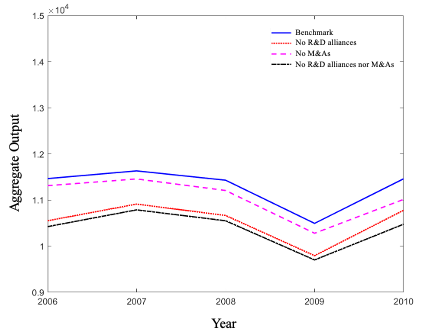
\includegraphics[width=5.25cm,angle=0]{./Figures/2006_2010_aggregated_2.png}
\end{minipage}
\begin{minipage}{0.33\linewidth}
\centering
\qquad 2011-2015
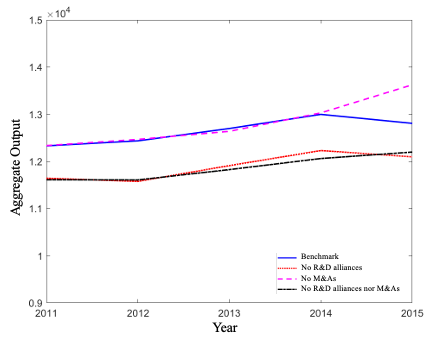
\includegraphics[width=5.5cm,angle=0]{./Figures/2011_2015_aggregated_2.png}
\end{minipage}
\begin{minipage}{0.32\linewidth}
\centering
\qquad 2016-2020
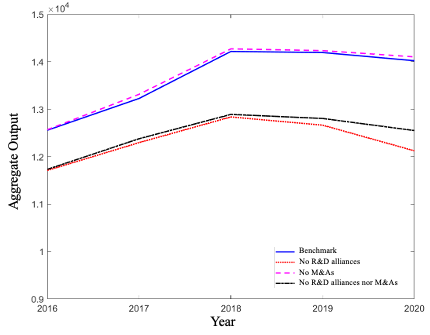
\includegraphics[width=5.25cm,angle=0]{./Figures/2016_2020_aggregated_2.png}
\end{minipage}
%
%
\begin{minipage}{0.32\linewidth}
\centering
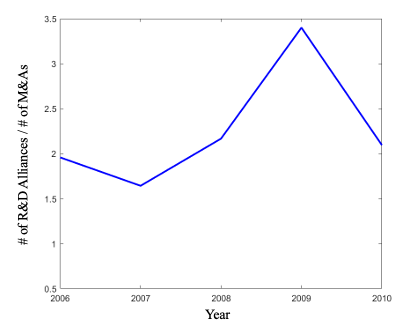
\includegraphics[width=5.25cm,angle=0]{./Figures/2006_2010_ratio_rnd_ma_2.png}
\end{minipage}
\begin{minipage}{0.33\linewidth}
\centering
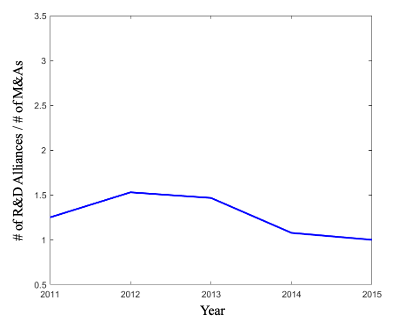
\includegraphics[width=5.5cm,angle=0]{./Figures/2011_2015_ratio_rnd_ma_2.png}
\end{minipage}
\begin{minipage}{0.33\linewidth}
\centering
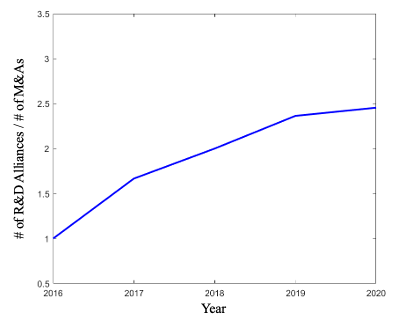
\includegraphics[width=5.5cm,angle=0]{./Figures/2016_2020_ratio_rnd_ma_2.png}
\end{minipage}
\caption{The top panels report counterfactual simulation results for the three sample periods showing the aggregate output under the benchmark and different counterfactual scenarios. The bottom panels display the ratio of the number of R\&D alliances to the number of M\&A deals. Solid lines: posterior medians; shaded areas: 90\% posterior predictive intervals across $S$ posterior draws (and network simulation draws in the re-equilibrated scenario).
}
\label{fig:counterfactual_aggregate}
\end{figure}
Figure~\ref{fig:counterfactual_aggregate} shows that the aggregate output loss from banning M\&A is large in 2006--2010 but substantially smaller in later periods, while removing R\&D alliances leads to persistently large losses throughout. At the same time, the bottom panels indicate that the intensity of collaborations relative to M\&A activity is higher in the early period. Taken together, these patterns reflect the payoff complementarity of Section~\ref{sec:model-implications}: accumulated alliance capital raises the surplus from consolidation, so periods of dense collaboration are followed by intense M\&A activity, even though, on the choice margin, each transaction is executed as a merger instead of an alliance. It also shows that when firms are embedded in dense collaboration networks, mergers can internalize and scale existing complementarities, resulting in large aggregate gains. As collaboration intensity per deal declines over time, there is less relational capital to internalize, reducing the marginal contribution of M\&A and explaining the smaller output losses from banning mergers in later periods.

%%%%%%%%%%%%%%%%%%%%%%%%%%%%%%%%%%%%%%%%%%%%%%%%%%%%%%%%%
\subsection{Deal-Level Counterfactual Effects}
%%%%%%%%%%%%%%%%%%%%%%%%%%%%%%%%%%%%%%%%%%%%%%%%%%%%%%%%%
\begin{figure}[tbp]
\begin{minipage}{0.32\linewidth}
\centering
\qquad 2006-2010
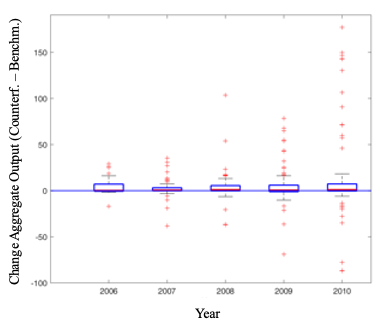
\includegraphics[width=5.25cm,angle=0]{./Figures/2006_2010_deal_level_2.png}
\end{minipage}
\begin{minipage}{0.33\linewidth}
\centering
\qquad 2011-2015
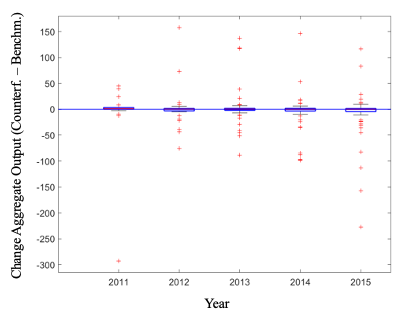
\includegraphics[width=5.75cm,angle=0]{./Figures/2011_2015_deal_level_2.png}
\end{minipage}
\begin{minipage}{0.3\linewidth}
\centering
\qquad 2016-2020
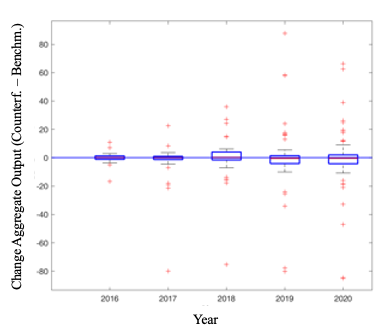
\includegraphics[width=5.25cm,angle=0]{./Figures/2016_2020_deal_level_2.png}
\end{minipage}
%\begin{minipage}{0.32\linewidth}
%\centering
%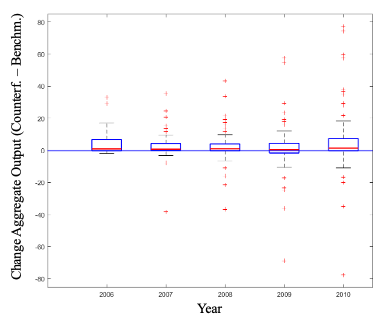
\includegraphics[width=5.6cm,angle=0]{./Figures/2006_2010_deal_level_no_RND_2.png}
%\end{minipage}
%\begin{minipage}{0.33\linewidth}
%\centering
%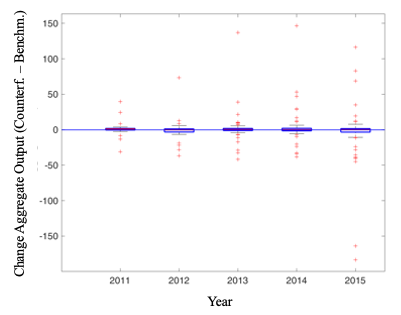
\includegraphics[width=5.5cm,angle=0]{./Figures/2011_2015_deal_level_no_RND_2.png}
%\end{minipage}
%\begin{minipage}{0.33\linewidth}
%\centering
%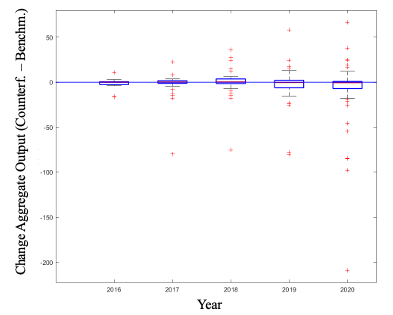
\includegraphics[width=5.6cm,angle=0]{./Figures/2016_2020_deal_level_no_RND_2.png}
%\end{minipage}
\caption{Individual merger-level counterfactual simulation results for the three sample periods when individual M\&A deals are prohibited. Solid lines: posterior medians; shaded areas: 90\% posterior predictive intervals across $S$ posterior draws (and network simulation draws in the re-equilibrated scenario).}
\label{fig:counterfactual_firm}
\end{figure}
Figure~\ref{fig:counterfactual_firm} highlights substantial heterogeneity in merger-level effects, with both positive and negative contributions reflecting variation in underlying complementarities across deals. The distribution is shifted upward in 2006--2010, indicating large average gains from M\&A, but becomes increasingly compressed around zero in later periods, pointing to weaker marginal effects. This pattern is consistent with differences in the surrounding collaboration environment: in the early period, a higher intensity of R\&D alliances per M\&A deal reported in the bottom panels in Figure~\ref{fig:counterfactual_aggregate} implies that firms are embedded in richer networks, allowing mergers to internalize and amplify existing complementarities \citep[][]{friedmann2026knowledge}. As the relative prevalence of alliances declines over time, the scope for such gains diminishes, leading to smaller and more dispersed merger effects.

%%%%%%%%%%%%%%%%%%%%%%%%%%%%%%%%%%%%%%%%%%%%%%%%%%%%%%%%%
\subsection{Sectoral Variation: ICT and Semiconductors vs. Biotech and Pharmaceuticals}
%%%%%%%%%%%%%%%%%%%%%%%%%%%%%%%%%%%%%%%%%%%%%%%%%%%%%%%%%

%%%%%%%%%%%%%%%%%%%%%%%%%%%%%%%%%%%%%%%%%%%%%%%%%%%%%%%%%
\subsection{Geographic Variation: United States vs. Europe}
%%%%%%%%%%%%%%%%%%%%%%%%%%%%%%%%%%%%%%%%%%%%%%%%%%%%%%%%%

\FloatBarrier

%%%%%%%%%%%%%%%%%%%%%%%%%%%%%%%%%%%%%%%%%%%%%%%%%%%%%%%%%
\section{Conclusion}
\label{sec:conclusion}
%%%%%%%%%%%%%%%%%%%%%%%%%%%%%%%%%%%%%%%%%%%%%%%%%%%%%%%%%
We estimate an R\&D network formation model using a novel dataset on R\&D collaborations extracted using natural language processing (NLP) from news articles over several decades. We find that technology spillovers in R\&D collaborations have changed over time. %The changing pattern in technology spillovers motivates us to include M\&A activities in our estimation framework. 
Our results indicate that the changing pattern in technology spillovers is due to firms substituting R\&D collaborations with M\&A,\footnote{Throughout the paper, the relation between R\&D collaborations and
M\&As involves two distinct notions that it is important to keep apart.
On the \emph{ex-ante choice margin}, the two governance modes are
substitutes by construction: for a given pair and period, acquiring,
collaborating, and remaining idle are mutually exclusive alternatives
in the discrete choice of Section~\ref{sec:dyn-rnd-mna}, and the
threshold condition in Equation~(\ref{eq:rnd-mna-comp}) determines
which mode is selected. Any factor that raises the relative
attractiveness of one mode mechanically lowers the probability of the
other; in particular, removing the acquisition alternative reallocates
its choice probability to collaboration and idleness
(Online Appendix~\ref{app:equivalence}). In the \emph{payoff structure},
by contrast, the two modes are dynamic complements: a prior alliance
and common collaboration partners lower the cost of a subsequent
acquisition when $\kappa_{9} < \gamma_{5}$ and
$\kappa_{10} < \gamma_{6}$ in
Equation~(\ref{eq:mna_rnd_cost-diff}), 
and the target's alliance portfolio is part of the transferable network
value that makes it worth acquiring
(Equation~(\ref{eq:mna-form-profit})). Alliance capital accumulated
today therefore raises the surplus from consolidation tomorrow --- the
stepping-stone mechanism --- even though, at the moment of choice, one
mode is always selected \emph{instead of} the other. When we speak of
firms ``substituting collaborations with M\&As'' we refer to the choice
margin; when we speak of alliances and M\&As as ``complements'' we
refer to the payoff structure. The two notions are not in tension: it
is precisely because alliance capital raises merger surplus that, over
time, activity shifts along the choice margin from collaboration
toward consolidation.} emphasizing the close connection between R\&D collaborations and M\&A activities. Moreover, a counterfactual analysis indicates that banning M\&As unanimously reduce aggregate firm output, while R\&D alliances increase aggregate firm output. %We acknowledge that mergers may also have positive benefits by reducing ex post hold-up costs. We are extending the model to allow for mergers to also benefit firms by reducing duplicative R\&D costs and by allowing firms to reduce ex post holdup costs as in \cite{williamson1998institutions} through integrating.  

\end{spacing}

\singlespacing

%%%%%%%%%%%%%%%%%%%%%%%%%%%%%%%%%%%%%%%%%%%%%%%%%%%%%%%%%
\begin{spacing}{0.75}
\bibliographystyle{apalike}
\bibliography{references}
\end{spacing}

\clearpage

%%%%%%%%%%%%%%%%%%%%%%%%%%%%%%%%%%%%%%%%%%%%%%%%%%%%%%%%%
\section*{Appendix}
\appendix

\setcounter{section}{0}
\setcounter{page}{1}

% Appendix section numbering: A, B, C, ...
\renewcommand{\thesection}{\Alph{section}}
% Appendix subsection numbering: A.1, A.2, B.1, ...
\renewcommand{\thesubsection}{\thesection.\arabic{subsection}}
\renewcommand{\thesubsubsection}{\thesubsection.\arabic{subsubsection}}
% Equation numbering within appendix sections: A.1, A.2, B.1, ...
\numberwithin{equation}{section}
\renewcommand{\theequation}{\thesection.\arabic{equation}}
% Optional: figure and table numbering as Figure A.1, Table A.1, etc.
\renewcommand{\thefigure}{\thesection.\arabic{figure}}
\renewcommand{\thetable}{\thesection.\arabic{table}}
\makeatletter
\@addtoreset{figure}{section}
\@addtoreset{table}{section}
\makeatother
\singlespacing

%%%%%%%%%%%%%%%%%%%%%%%%%%%%%%%%%%%%%%%%%%%%%%%%%%%%%%%%%
\section{Notation}
\label{app:notation}
%%%%%%%%%%%%%%%%%%%%%%%%%%%%%%%%%%%%%%%%%%%%%%%%%%%%%%%%%
Table~\ref{tab:notation-main} collects the notation of the main text and %Table~\ref{tab:notation-app} 
the symbols whose meaning is local to individual
appendices. 
%Several symbols are deliberately reused across scopes and
%are flagged in the notes to the table: $\kappa$ (the product-market
%dampening factor of Equation~\eqref{eq:single-market-elements} vs.\ the
%M\&A cost parameters $\kappa_0,\kappa_1,\dots$ of
%Equation~\eqref{eq:mna-cost}), $m$ (the kernel entries $m_{ij}$ vs.\ the
%merger indicators $m_{ij,t}$), $\mathbf{c}$ (Katz--Bonacich centrality
%vs.\ the dyadic covariate vector $\mathbf{c}_{ij,t}$), $\delta$ (the
%depreciation rate of Equation~\eqref{eq:rnd-accumulation}, and $x,y,\alpha,\nu,\gamma$
%(whose appendix-local meanings in Appendices~\ref{sec:micro-cost}
%and~\ref{sec:mat-perturb} differ from their main-text meanings).

\begin{table}[htbp]
\vspace{-2cm}
\centering
\scalebox{0.8}{
\begin{threeparttable}
\caption{\label{tab:notation-main} Notation in main text.}
{\footnotesize
\begin{tabular}{@{} l l l @{}}
\toprule
Symbol & Meaning & Defined in \\
\midrule
$n$; $i,j,k,\ell$ & number of firms; firm indices & Sec.~\ref{sec:model-profits} \\
$G_t$; $\mathbf{A}_t=(a_{ij,t})$ & R\&D collaboration network; its adjacency matrix & Sec.~\ref{sec:model-profits} \\
$\mathbf{B}=(b_{ij,t})$ & product-market competition matrix (TNIC) & Sec.~\ref{sec:industry}, \ref{sec:model-profits} \\
$\mathcal{M}_k$ & product market $k$ & Sec.~\ref{sec:model-profits} \\
$y_{it}$, $\mathbf{y}_t$ & equilibrium output & Eq.~\eqref{eq:output-br} \\
$\eta_{it}$, $\bm{\eta}_t$ & productivity & Eq.~\eqref{eq:prod-dyn} \\
$x_{it}$; $R_{it}$ & R\&D capital stock; R\&D investment & Eq.~\eqref{eq:rnd-accumulation} \\
$\delta$ & depreciation rate of R\&D capital ($=0.15$) & Eq.~\eqref{eq:rnd-accumulation} \\
$\lambda$; $\rho$ & product-market rivalry; technology-spillover parameter & Eq.~\eqref{eq:profit-simplified} \\
$\theta=(\rho,\lambda)$ & spillover and competition parameters & Sec.~\ref{sec:dyn-rnd} \\
$\xi$ & profit scale parameter, normalized to one$^{a}$ & Eq.~\eqref{eq:profit-simplified} \\
$\psi$; $\upsilon$ & demand curvature; market size & Sec.~\ref{sec:model-profits}, App.~\ref{sec:cournot} \\
$\pi_i$; $\Pi$; $U$; $W$ & firm profit; producer surplus; consumer surplus; welfare & Eqs.~\eqref{eq:profit-simplified}, \eqref{eq:profit-eq} \\
$H_k$ & Herfindahl--Hirschman index of market $k$ & Sec.~\ref{sec:model-profits}, Eq.~\eqref{eq:herfindahl} \\
$\mathbf{S}_t=\mathbf{I}_n+\lambda\mathbf{B}-\rho\mathbf{A}_t$ & interaction matrix & Eq.~\eqref{eq:bonacich} \\
$\mathbf{M}=(m_{ij})=\mathbf{S}^{-1}$ & equilibrium (interaction) kernel$^{b}$ & Eq.~\eqref{eq:bonacich}, Sec.~\ref{sec:model-implications} \\
$m_{ij,t}$; $M_t$ & merger indicator ($i$ acquires $j$); set of deals$^{b}$ & Sec.~\ref{sec:dyn-rnd-mna}, Tab.~\ref{tab:outcomes-seq} \\
$a_{ij,t}$ & R\&D collaboration indicator & Eq.~\eqref{eq:profit-simplified} \\
$\zeta_{ij,t}$; $\gamma=(\gamma_0,\gamma_1,\dots)$ & R\&D collaboration cost; its parameters$^{c}$ & Eq.~\eqref{eq:link-cost} \\
$\nu_{ij,t}$; $\kappa=(\kappa_0,\kappa_1,\dots)$ & M\&A transaction cost; its parameters$^{c,d}$ & Eq.~\eqref{eq:mna-cost} \\
$\mathbf{c}_{ij,t}$ & dyadic covariates (TNIC similarity, etc.)$^{e}$ & Eq.~\eqref{eq:link-cost} \\
$\varepsilon^{\text{M\&A}}_{ij,t}$, $\varepsilon^{\text{R\&D}}_{ij,t}$, $\varepsilon^{\text{ID}}_{i,t}$ & type~I extreme value payoff shocks & Sec.~\ref{sec:dyn-rnd-mna} \\
$\Pi^{\text{M\&A}}_{ijt}$, $\Pi^{\text{R\&D}}_{ijt}$, $\Pi^{\text{ID}}_{it}$ & deterministic first-stage payoffs & Eq.~\eqref{eq:profit-mna}, Sec.~\ref{sec:dyn-rnd} \\
$p^{\mathrm{ac}}_{ij,t}$; $q_{ij,t}$ & acquisition prob.; conditional collaboration prob. & Eqs.~\eqref{eq:i-ac-j}, \eqref{eq:i-co-j} \\
$\mathbf{H}=(h_{ij})$; $\phi=\rho/(1-\lambda)$ & Katz--Bonacich kernel $(\mathbf{I}_n-\phi\mathbf{A})^{-1}$; decay factor & Sec.~\ref{sec:model-implications}, App.~\ref{sec:katz-bonacich} \\
$c_i$, $\mathbf{c}=\mathbf{H}\mathbf{u}$ & Katz--Bonacich centrality$^{e}$ & Sec.~\ref{sec:model-implications} \\
$\kappa$ & product-market dampening factor$^{c}$ & Eq.~\eqref{eq:single-market-elements} \\
$y^{+ij}_{it}$; $y^{ac,ij}_{it}$ & post-collaboration; post-acquisition output & Eqs.~\eqref{eq:post-link-output-i}, \eqref{eq:mna-form-profit} \\
$\widehat{\mathbf{A}}^{\,ij}$, $\widehat{\mathbf{M}}^{\,ij}$ & post-reassignment adjacency matrix and kernel & Eq.~\eqref{eq:adjacency-reassignment-mna} \\
$\widetilde{\mathbf{A}}^{\,ij}$, $\widetilde{\mathbf{M}}^{\,ij}$ & post-removal adjacency matrix and kernel & Eq.~\eqref{eq:post-removal-weight-mna} \\
$\bm{\eta}^{ac,ij}_t$ & post-acquisition productivity vector & Eq.~\eqref{eq:prod-mna-alt} \\
$\Theta=(\theta,\beta,\gamma,\kappa,\mu,\tau,\sigma^2_v)$ & full parameter vector & Sec.~\ref{sec:estimation-algorithm} \\
$\beta$; $\mu_i$; $\tau_t$; $v_{it}$; $\sigma^2_v$ & productivity coefficients; firm and time effects; shock & Eq.~\eqref{eq:prod-dyn} \\
$I(\cdot)$; $I^{0}_{ij,t}$ & indicator function; idle-pair indicator & Eq.~\eqref{eq:mna-rnd-joint} \\
$\mathbf{u}$; $\mathbf{e}_i$ & vector of ones; $i$-th unit basis vector & Sec.~\ref{sec:dyn-rnd}, \ref{sec:model-implications} \\
$x_i$; $y_i$ & output; R\&D effort in the micro-foundation$^{f}$ & App.~\ref{sec:cournot} \\
$\alpha$; $\beta$ & own and partner R\&D cost-reduction parameters$^{f}$ & Eq.~\eqref{eq:marginal-cost} \\
$\gamma$; $\nu=\psi-\alpha^2/(4\gamma)$ & R\&D effort cost; own-concavity parameter$^{f}$ & Eq.~\eqref{eq:profit-pi-app-3} \\
$\bar c_i$; $p_i$; $E_k$, $I_k$ & marginal cost; price; endowment and numeraire & Eqs.~\eqref{eq:marginal-cost}, \eqref{eq:inverse-demand}, \eqref{eq:utility} \\
$\mathbf{b}_{\mathbf{u}}$, $\mathbf{b}_{\bm{\eta}}$ & unweighted and $\bm{\eta}$-weighted Katz--Bonacich vectors & Eq.~\eqref{eq:bonacich-centrality}, App.~\ref{sec:nash-katz} \\
$\lambda_{\max}$, $\mathbf{v}_1$ & largest eigenvalue and Perron vector of $\mathbf{A}$ & App.~\ref{sec:katz-bonacich} \\
$\mathbf{W}=\rho\mathbf{A}-\lambda\mathbf{B}$; $r(\cdot)$ & signed net-interaction matrix; spectral radius & Eq.~\eqref{eq:neumann-kernel}, App.~\ref{sec:br} \\
$\alpha$; $\Delta$ & rank-two perturbation weight; capacitance determinant$^{f}$ & Lem.~\ref{lem:matrix-perturbation-inv} \\
$\mathbf{U}$, $\mathbf{V}$, $\mathbf{W}$ & Woodbury factors and capacitance matrix & Eqs.~\eqref{eq:woodbury-sylvester}, \eqref{eq:merger-update} \\
$\mathbf{u}=\mathbf{e}_i-\mathbf{e}_j$; $\mathbf{c}$ & merger transfer vector; common-collaborator profile$^{e}$ & Lem.~\ref{lem:matrix-perturbation-mult-swap} \\
$\mathbf{M}$, $\widetilde{\mathbf{y}}$ & interaction matrix and iterate in best-response updating & Eq.~\eqref{eq:output-iteration}, App.~\ref{sec:br-part} \\
$s_{ij,t}$ & announcement of firm $i$ toward firm $j$ & Eq.~\eqref{eq:app:actions} \\
$\mathbb{P}^{\mathrm{sim}}$, $\mathbb{P}^{\mathrm{seq}}$, $\mathbb{P}^{\mathrm{comp}}$ & simultaneous, sequential and composite likelihoods & Eqs.~\eqref{eq:app:liksim}, \eqref{eq:mna-rnd-joint}, \eqref{eq:app:comppair} \\
$\omega_{ij,t}$ & control-contest ratio & Eq.~\eqref{eq:app:omega} \\
$\Lambda_t$; $\mu_t$; $\bar p_t$, $\bar q_t$ & expected contests; expected announcements; maxima & Eq.~\eqref{eq:app:Lambda} \\
$d_{\mathrm{TV}}$ & total-variation distance & Prop.~\ref{prop:app:composite} \\
\midrule
\bottomrule
\end{tabular}
}
\begin{tablenotes}[flushleft]
\item \small $^{a}$ The profit-scale parameter in $\xi$ is normalized to one in Section~\ref{sec:dyn-rnd}, which is equivalent to expressing $\zeta_{ij,t}$ and $\nu_{ij,t}$ relative to $\xi$.
$^{b}$ Kernel entries $m_{ij}$ carry no time subscript; merger
indicators $m_{ij,t}$ always do.
$^{c}$ The scalar dampening factor $\kappa$ of
Eq.~\eqref{eq:single-market-elements} is an equilibrium object
determined by $\lambda$ and the network; the M\&A cost parameters
$\kappa_0,\kappa_1,\dots$ of Eq.~\eqref{eq:mna-cost} always carry a
numeric subscript. The same convention distinguishes the collaboration
cost parameters $\gamma_0,\gamma_1,\dots$ from the R\&D effort cost
$\gamma$ of Appendix~\ref{sec:cournot}.
$^{d}$ The specification estimated in
Table~\ref{tab:result_output_US_compustat_NAICS_6_mna} augments
Eqs.~\eqref{eq:link-cost} and~\eqref{eq:mna-cost} by further dyadic
covariates (patent and vertical-relatedness similarity, the TNIC
similarity--HHI interaction, and acquirer and target patent stocks); the
parameter indices in that table follow the notes to the table.
$^{e}$ The centrality vector $\mathbf{c}$ carries a single firm subscript
($c_i$); the dyadic covariate vector $\mathbf{c}_{ij,t}$ always carries a
pair--time subscript; the common-collaborator profile $\mathbf{c}$ of
Lemma~\ref{lem:matrix-perturbation-mult-swap} is local to
Appendix~\ref{sec:mat-perturb}.
$^{f}$ The symbols $x_i$, $y_i$, $\alpha$, $\beta$, $\gamma$ and $\nu$ in
Appendix~\ref{sec:micro-cost} are local to the micro-foundation and
unrelated to their main-text meanings; the mapping to the main text sets
$\nu=\tfrac{1}{2}$ and relabels output $x_i$ as $y_i$ (see
Eqs.~\eqref{eq:profit-pi-app-3} and~\eqref{eq:output-br-app}). The
symbol $\alpha$ additionally denotes the generic weight of a symmetric
rank-two perturbation in Lemma~\ref{lem:matrix-perturbation-inv}.
\end{tablenotes}
\end{threeparttable}}
\end{table}

%\begin{table}[htbp]
%\centering
%\scalebox{1}{
%\begin{threeparttable}
%\caption{\label{tab:notation-app} Appendix-local symbols.}
%{\footnotesize
%\begin{tabular}{@{} l l l @{}}
%\toprule
%Symbol & Meaning & Defined in \\
%\midrule
%$x_i$; $y_i$ & output; R\&D effort in the micro-foundation$^{f}$ & App.~\ref{sec:cournot} \\
%$\alpha$; $\beta$ & own and partner R\&D cost-reduction parameters$^{f}$ & Eq.~\eqref{eq:marginal-cost} \\
%$\gamma$; $\nu=\psi-\alpha^2/(4\gamma)$ & R\&D effort cost; own-concavity parameter$^{f}$ & Eq.~\eqref{eq:profit-pi-app-3} \\
%$\bar c_i$; $p_i$; $E_k$, $I_k$ & marginal cost; price; endowment and numeraire & Eqs.~\eqref{eq:marginal-cost}, \eqref{eq:inverse-demand}, \eqref{eq:utility} \\
%$\mathbf{b}_{\mathbf{u}}$, $\mathbf{b}_{\bm{\eta}}$ & unweighted and $\bm{\eta}$-weighted Katz--Bonacich vectors & Eq.~\eqref{eq:bonacich-centrality}, App.~\ref{sec:nash-katz} \\
%$\lambda_{\max}$, $\mathbf{v}_1$ & largest eigenvalue and Perron vector of $\mathbf{A}$ & App.~\ref{sec:katz-bonacich} \\
%$\mathbf{W}=\rho\mathbf{A}-\lambda\mathbf{B}$; $r(\cdot)$ & signed net-interaction matrix; spectral radius & Eq.~\eqref{eq:neumann-kernel}, App.~\ref{sec:br} \\
%$\alpha$; $\Delta$ & rank-two perturbation weight; capacitance determinant$^{f}$ & Lem.~\ref{lem:matrix-perturbation-inv} \\
%$\mathbf{U}$, $\mathbf{V}$, $\mathbf{W}$ & Woodbury factors and capacitance matrix & Eqs.~\eqref{eq:woodbury-sylvester}, \eqref{eq:merger-update} \\
%$\mathbf{u}=\mathbf{e}_i-\mathbf{e}_j$; $\mathbf{c}$ & merger transfer vector; common-collaborator profile$^{e}$ & Lem.~\ref{lem:matrix-perturbation-mult-swap} \\
%$\mathbf{M}$, $\widetilde{\mathbf{y}}$ & interaction matrix and iterate in best-response updating & Eq.~\eqref{eq:output-iteration}, App.~\ref{sec:br-part} \\
%$s_{ij,t}$ & announcement of firm $i$ toward firm $j$ & Eq.~\eqref{eq:app:actions} \\
%$\mathbb{P}^{\mathrm{sim}}$, $\mathbb{P}^{\mathrm{seq}}$, $\mathbb{P}^{\mathrm{comp}}$ & simultaneous, sequential and composite likelihoods & Eqs.~\eqref{eq:app:liksim}, \eqref{eq:mna-rnd-joint}, \eqref{eq:app:comppair} \\
%$\omega_{ij,t}$ & control-contest ratio & Eq.~\eqref{eq:app:omega} \\
%$\Lambda_t$; $\mu_t$; $\bar p_t$, $\bar q_t$ & expected contests; expected announcements; maxima & Eq.~\eqref{eq:app:Lambda} \\
%$d_{\mathrm{TV}}$ & total-variation distance & Prop.~\ref{prop:app:composite} \\
%\midrule
%\bottomrule
%\end{tabular}
%}
%\begin{tablenotes}[flushleft]
%%\item \small $^{a}$ The depreciation rate $\delta$ in
%%Equation~\eqref{eq:rnd-accumulation} is distinct from the profit-scale
%%parameter in $\xi=\exp(\delta)$; the latter is normalized to one in
%%Section~\ref{sec:dyn-rnd}, which is equivalent to expressing
%%$\zeta_{ij,t}$ and $\nu_{ij,t}$ relative to $\xi$.
%%$^{b}$ Kernel entries $m_{ij}$ carry no time subscript; merger
%%indicators $m_{ij,t}$ always do.
%%$^{c}$ The scalar dampening factor $\kappa$ of
%%Equation~\eqref{eq:single-market-elements} is an equilibrium object
%%determined by $\lambda$ and the network; the M\&A cost parameters
%%$\kappa_0,\kappa_1,\dots$ of Equation~\eqref{eq:mna-cost} always carry a
%%numeric subscript. The same convention distinguishes the collaboration
%%cost parameters $\gamma_0,\gamma_1,\dots$ from the R\&D effort cost
%%$\gamma$ of Appendix~\ref{sec:cournot}.
%%$^{d}$ The specification estimated in
%%Table~\ref{tab:result_output_US_compustat_NAICS_6_mna} augments
%%Equations~\eqref{eq:link-cost} and~\eqref{eq:mna-cost} by further dyadic
%%covariates (patent and vertical-relatedness similarity, the TNIC
%%similarity--HHI interaction, and acquirer and target patent stocks); the
%%parameter indices in that table follow the notes to the table.
%\item \small $^{e}$ The centrality vector $\mathbf{c}$ carries a single firm subscript
%($c_i$); the dyadic covariate vector $\mathbf{c}_{ij,t}$ always carries a
%pair--time subscript; the common-collaborator profile $\mathbf{c}$ of
%Lemma~\ref{lem:matrix-perturbation-mult-swap} is local to
%Appendix~\ref{sec:mat-perturb}.
%$^{f}$ The symbols $x_i$, $y_i$, $\alpha$, $\beta$, $\gamma$ and $\nu$ in
%Appendix~\ref{sec:micro-cost} are local to the micro-foundation and
%unrelated to their main-text meanings; the mapping to the main text sets
%$\nu=\tfrac{1}{2}$ and relabels output $x_i$ as $y_i$ (see
%Equations~\eqref{eq:profit-pi-app-3} and~\eqref{eq:output-br-app}). The
%symbol $\alpha$ additionally denotes the generic weight of a symmetric
%rank-two perturbation in Lemma~\ref{lem:matrix-perturbation-inv}.
%\end{tablenotes}
%\end{threeparttable}}
%\end{table}

\FloatBarrier

%%%%%%%%%%%%%%%%%%%%%%%%%%%%%%%%%%%%%%%%%%%%%%%%%%%%%%%%%
\section{Cost Reducing R\&D Collaborations}
\label{sec:micro-cost}
%%%%%%%%%%%%%%%%%%%%%%%%%%%%%%%%%%%%%%%%%%%%%%%%%%%%%%%%%
In the following we derive the firm's profit function in Equations (\ref{eq:profit-simplified}) or (\ref{eq:profit-eq}), respectively, and the corresponding best response function in Equation (\ref{eq:output-br}) %in Section \ref{sec:model} 
from a Cournot competition model (Appendix  \ref{sec:cournot}) or a Bertrand competition model (Appendix \ref{sec:bertrand}) with cost reducing R\&D collaborations.\footnote{See also \citet[][]{goyal01:_r_d_networ}, \citet[][]{Konig2018} and \citet[][]{Hsieh2021}.}

%%%%%%%%%%%%%%%%%%%%%%%%%%%%%%%%%%%%%%%%%%%%%%%%%%%%%%%%%
\subsection{Cournot Competition}
\label{sec:cournot}
%%%%%%%%%%%%%%%%%%%%%%%%%%%%%%%%%%%%%%%%%%%%%%%%%%%%%%%%%
We consider a Cournot oligopoly game in which a set $\mathcal{N}=\{1,\dots,n\}$ of firms is competing in a product market with imperfectly substitutable goods. 
Firms are not only competitors in the product market, but they can also form pairwise collaborative R\&D agreements. 
These pairwise links
involve a commitment to share R\&D results and lead to lower marginal
cost of production of the collaborating firms. 
%\footnote{R\&D partnerships have become a widespread phenomenon characterizing technological dynamics, especially in industries with rapid technological development such as, for instance, the pharmaceutical and chemical industries
%\citep[see e.g.][]{hagedoorn02:_inter_r_d,
%roijakkers06:_inter_r_d, powell05:_networ_dynam_field_evolut}. In these
%industries firms have become more specialized in specific domains of a
%technology and they tend to combine their knowledge with that of other firms
%that are specialized in different domains in order to jointly generate innovations that can help to develop new products or reduce their production
%costs \citep{ahuja00:_collab, powell96:_inter_collab_and_locus_of_innov}.
%For example, \citet{Bernstein1988} finds that R\&D spillovers decrease the
%unit costs of production for a sample of Canadian firms. Similarly \citet{Belderbos2004} find evidence for production cost reductions due to R\&D collaborations using data on a large sample of Dutch innovating firms.}
The amount of this cost reduction depends on the effort the firms invest into R\&D. Given the collaboration network $G \in \mathcal{G}^n$, where $\mathcal{G}^n$ denotes the set of all graphs with $n$ nodes, and the firms' R\&D effort levels, $\mathbf{y} = (y_i)_{i=1}^n$, the marginal cost of production for firm $i$ is given by \citep[cf.][]{goyal01:_r_d_networ}%\footnote{This generalizes earlier studies such as the one by \citet{aspremont88:_cooper_and_noncoop_r_d} where spillovers were assumed to take place between all firms in the industry and no distinction between collaborating and non-collaborating firms was made.}
\begin{equation}
c_i = \bar{c}_i - \alpha y_i - \beta \sum_{j=1}^n a_{ij} y_j.
\label{eq:marginal-cost}
\end{equation}
The indicator variables $a_{ij} \in \{0,1\}$ in Equation (\ref{eq:marginal-cost}) indicate wether firms $i$ and $j$ are collaborating (or not), and can be represented by the symmetric adjacency matrix $\mathbf{A}=(a_{ij})_{1\le i,j \le n}$ (with zero diagonal, $a_{ii}=0$). The parameter $\alpha \ge 0$ \label{sym:alpha} measures the
relative cost reduction due to a firms' own R\&D effort while the parameter $\beta \ge 0$ \label{sym:beta} measures the relative cost reduction due to
the R\&D effort of its collaboration partners. %\footnote{%
%Note that in this model, firms are exposed to business stealing effects if
%their rivals increase their output via cost reducing R\&D collaborations.}
%\footnote{In order to guarantee non-negative marginal costs we assume that $e_i \in [0, \bar{y}]$ and $\bar{c} \ge (n-1) \bar{e}$. This shows that $\bar{c}$ must be of the order of $O(n)$. Throughout the paper we shall assume parameter are constrained such that the second-order conditions hold and equilibria can be characterized in terms of first-order conditions and are interior.}
We further allow for ex ante heterogeneity (observed and unobserved) among firms in the cost parameter $\bar c_i \ge 0$
expressing their different technological and organizational capabilities related to heterogeneous firm productivities \citep[][]{Banerjee2005, Blundell1995}.

We further assume that firms incur a direct cost $\gamma y_{i}^{2}$, with $\gamma \ge 0$, for their R\&D effort and a fixed cost $\zeta_{ij} \ge 0$ for the R\&D collaboration between firms $i$ and $j$. The profit of firm $i$ is then given by
\begin{equation}
\pi_i = (p_i - c_i)x_i - \gamma y_i^2 - \sum_{j=1}^n a_{ij} \zeta_{ij},
\label{eq:profit-cost}
\end{equation}
where $x_i \ge 0$ is the output level and $\zeta_{ij}$ is the cost of collaboration between firms $i$ and $j$. Inserting marginal costs from Equation (\ref{eq:marginal-cost}) gives
\begin{equation*}
\pi_i = p_i x_i - \bar{c}_i x_i + \alpha x_i y_i +
\beta x_i \sum_{j=1}^n a_{ij} y_j - \gamma y_i^2 - \sum_{j=1}^n a_{ij}\zeta_{ij}.
\end{equation*}
Next we consider the demand for goods produced by firm $i$. A representative
consumer in market $\mathcal{M}_k \subseteq \mathcal{N}$, $k=1,\ldots,K$ maximizes \citep{Singh1984}
\begin{equation}
%U = I + \upsilon \sum_{i=1}^n x_i - \frac{\psi}{2} \sum_{i=1}^n x_i^2 - \frac{\lambda}{2} \sum_{i=1}^n \sum_{j \ne i}^n x_i x_j,
U_k = I_k + \upsilon \sum_{i \in \mathcal{M}_k} x_i - \frac{\psi}{2} \sum_{i \in \mathcal{M}_k} x_i^2 - \frac{\lambda}{2} \sum_{\substack{i,j \in \mathcal{M}_k, \\ j \neq i}} x_i x_j,
\label{eq:utility}
\end{equation}
with the budget constraint $I_k + \sum_{i \in \mathcal{M}_k} p_i x_i \le E_k$, endowment $E_k$ and a numeraire good $I_k$. The parameter $\upsilon>0$ captures the total
size of the market, whereas $\lambda \in (0,1]$, measures the degree of
substitutability between products. In particular, $\lambda = 1$ depicts a market
of perfect substitutable goods, while $\lambda \to 0$ represents the
case of almost independent markets. %\footnote{Observe that we do not ex ante impose any restrictions on the parameter $\lambda$, in particular, we do not require that $\lambda=1$ nor $\lambda=0$.}
The parameter $\lambda$ is therefore a measure of the degree of competition between firms. We assume that $\psi>\lambda>0$ to ensure that the utility function is concave. The budget constraint is binding and the utility maximization of the representative
consumer gives the inverse demand function for firm $i \in \mathcal{M}_k$:\footnote{With the budget constraint $I_k = E_k - \sum_{i \in \mathcal{M}_k} p_i x_i$ in the consumer's utility in Equation (\ref{eq:utility}), the FOC for $i \in \mathcal{M}_k$ is given by $\frac{\partial U_k}{\partial x_i} = - p_i + \upsilon - \psi x_i - \lambda \sum_{\substack{j \in \mathcal{M}_k, j \neq i}} ^n x_j = 0$, from which we obtain Equation (\ref{eq:inverse-demand}).}
\begin{equation}
p_i = \upsilon - \psi x_i - \lambda \sum_{j \in \mathcal{M}_k, j \neq i} x_j.
\label{eq:inverse-demand}
\end{equation} 
%Moreover, inserting Equation (\ref{eq:inverse-demand}) into the utility (\ref{eq:utility}) of the consumer gives: 
%\begin{align}
%U & = E - \sum_{i=1}^n p_i x_i + \upsilon \sum_{i=1}^n x_i - \frac{\psi}{2} \sum_{i=1}^n x_i^2 - \frac{\lambda}{2} \sum_{i=1}^n \sum_{j \ne i}^n x_i x_j \notag \\
%& = E - \sum_{i=1}^n \left( \upsilon - \psi x_i - \lambda \sum_{j \ne i}^n x_j \right) x_i + \upsilon \sum_{i=1}^n x_i - \frac{\psi}{2} \sum_{i=1}^n x_i^2 -\frac{\lambda}{2} \sum_{i=1}^n \sum_{j \ne i}^n x_i x_j \notag \\
%& = E + \frac{\psi}{2} \sum_{i=1}^n x_i^2 + \frac{\lambda}{2} \sum_{i=1}^n \sum_{j \ne i}^n x_i x_j. 
%\label{eq:consumer-utility}
%\end{align}
%This defines consumer surplus. Note that in the special case of non-substitutable goods, when $\lambda \to 0$, we obtain $U = E +\frac{\psi}{2} \sum_{i=1}^n x_i^2$, while in the case of perfectly substitutable goods, when $\lambda \to 1$, we get $U = E +\frac{1+\psi}{2} \left(\sum_{i=1}^n x_i \right)^2$. 
Inserting the marginal cost from Equation (\ref{eq:marginal-cost}) and inverse demand from Equation (\ref{eq:inverse-demand}) into profits yields
\begin{equation}
\pi_i = \upsilon  x_i - \psi x_i^2 - \lambda \sum_{j \ne i}^n b_{ij} x_j x_i - \bar{c}_i x_i + \alpha x_i y_i +
\beta x_i \sum_{j=1}^n a_{ij} y_j - \gamma y_i^2 - \sum_{j=1}^n a_{ij}\zeta_{ij},
\label{eq:profit-app}
\end{equation}
where $b_{ij} \in \{0,1\}$ is an indicator variable for whether firms $i$ and $j$ are competitors (or not), i.e. $i,j \in \mathcal{M}_k$ for some $k$. This can be represented by the symmetric block diagonal competition matrix $\mathbf{B}=(b_{ij})_{1\le i,j \le n}$. The optimal R\&D effort level follows from the first-order condition 
\begin{equation*}
\frac{\partial \pi_i}{\partial y_i} = \alpha x_i -2 \gamma y_i = 0.
\end{equation*}
Solving for $y_i$ delivers\footnote{%
We assume that firms always implement the optimal R\&D effort level. Since
the optimal R\&D effort decision only depends on a firm's own output, we
assume that a firm does not face any uncertainty when implementing this
strategy. %In contrast, in Section \ref{sec:stability} we will, however, introduce noise in the optimal output and collaboration decisions, since these depend on the decisions of all other firms in the industry and their characteristics, which might be harder to observe. 
See also \citet{kamien92:_resear_joint_ventur_and_r_d_cartel} for a similar
model of competitive research joint ventures in which firms unilaterally (and optimally) choose their R\&D
effort levels.}  
\begin{equation}
y_i = \frac{\alpha}{2 \gamma} x_i.
\label{eq:opt-rnd-effort}
\end{equation}
This equation can be viewed as reflecting learning-by-doing effects of production on R\&D. It is consistent with various empirical studies which have found
that the R\&D effort is correlated with firm size \citep{cohen96:_firm_size_and_natur_of, cohen96:_repris_of_size_and_r_d}. 

Similarly, the first-order condition w.r.t. to output, $x_i$, is given by
\begin{equation*}
\frac{\partial \pi_i}{\partial x_i} = \upsilon - 2 \psi x_i - \lambda \sum_{j \ne i}^n b_{ij} x_j - \bar{c}_i  + \alpha y_i +
\beta \sum_{j=1}^n a_{ij} y_j = 0.
\end{equation*}
This gives
\begin{equation*}
x_i = \frac{\upsilon - \bar{c}_i}{2 \psi}  - \frac{\lambda}{2 \psi} \sum_{j \ne i}^n b_{ij} x_j +  \frac{\alpha}{2 \psi} y_i +
\frac{\beta}{2 \psi} \sum_{j=1}^n a_{ij} y_j.
\end{equation*}
Further, inserting Equation (\ref{eq:opt-rnd-effort}) yields
\begin{equation*}
x_i = \frac{\upsilon - \bar{c}_i}{2 \psi}  - \frac{\lambda}{2 \psi} \sum_{j \ne i}^n b_{ij} x_j +  \frac{\alpha^2}{4 \psi \gamma} x_i +
\frac{\alpha \beta}{4 \psi \gamma} \sum_{j=1}^n a_{ij} x_j .
\end{equation*}
Solving for $x_i$ then gives
%\begin{equation*}
%(1- \frac{\alpha^2}{4 \psi \gamma} )x_i = \frac{\upsilon - \bar{c}_i}{2 \psi}  - \frac{\lambda}{2 \psi} \sum_{j \ne i}^n b_{ij} x_j +
%\frac{\alpha \beta}{4 \psi \gamma} \sum_{j=1}^n a_{ij} x_j.
%\end{equation*}
%and
%\begin{equation*}
%\frac{4 \psi \gamma-\alpha^2}{4 \psi \gamma} x_i = \frac{\upsilon - \bar{c}_i}{2 \psi}  - \frac{\lambda}{2 \psi} \sum_{j \ne i}^n b_{ij} x_j +
%\frac{\alpha \beta}{4 \psi \gamma} \sum_{j=1}^n a_{ij} x_j.
%\end{equation*}
%and
%\begin{equation*}
%x_i = \frac{4 \psi \gamma} {4 \psi \gamma-\alpha^2} \frac{\upsilon - \bar{c}_i}{2 \psi}  - \frac{4 \psi \gamma} {4 \psi \gamma-\alpha^2} \frac{\lambda}{2 \psi} \sum_{j \ne i}^n b_{ij} x_j +
%\frac{4 \psi \gamma} {4 \psi \gamma-\alpha^2} \frac{\alpha \beta}{4 \psi \gamma} \sum_{j=1}^n a_{ij} x_j.
%\end{equation*}
%and
\begin{equation}
x_i = \frac{2 \gamma (\upsilon - \bar{c}_i)} {4 \psi \gamma-\alpha^2} - \frac{2 \lambda \gamma} {4 \psi \gamma-\alpha^2} \sum_{j \ne i}^n b_{ij} x_j +
\frac{\alpha \beta} {4 \psi \gamma-\alpha^2} \sum_{j=1}^n a_{ij} x_j.
\label{eq:output-x-br-app}
\end{equation}
%If we denote by
%\begin{align*}
%\eta_i & \equiv \frac{2 \gamma (\upsilon - \bar{c}_i)} {4 \psi \gamma-\alpha^2} , \\
%\tilde{\lambda} &  \equiv \frac{2 \lambda \gamma} {4 \psi \gamma-\alpha^2} ,  \\
%\rho & \equiv\frac{\alpha \beta} {4 \psi \gamma-\alpha^2},
%\end{align*}
%then we get
%\begin{equation*}
%x_i = \eta_i - \tilde{\lambda} \sum_{j \ne i}^n b_{ij} x_j + \rho \sum_{j=1}^n a_{ij} x_j,
%\end{equation*}
%Multiplication with $\frac{\alpha}{2\gamma}$ and using Equation (\ref{eq:opt-rnd-effort}) this can be written equivalently in terms of R\&D effort as follows
%\begin{equation*}
%y_i = \frac{\alpha (\upsilon - \bar{c}_i)} {4 \psi \gamma-\alpha^2} - \frac{2 \lambda \gamma} {4 \psi \gamma-\alpha^2} \sum_{j \ne i}^n b_{ij} y_j +
%\frac{\alpha \beta} {4 \psi \gamma-\alpha^2} \sum_{j=1}^n a_{ij} y_j.
%\end{equation*}
%If we denote by
%\begin{align*}
%\eta_i & \equiv \frac{\alpha (\upsilon - \bar{c}_i)} {4 \psi \gamma-\alpha^2}, \\
%\tilde{\lambda} &  \equiv \frac{2 \lambda \gamma} {4 \psi \gamma-\alpha^2},  \\
%\rho &  \equiv \frac{\alpha \beta} {4 \psi \gamma-\alpha^2} ,
%\end{align*}
%then we get
%\begin{equation*}
%y_i = \eta_i - \tilde{\lambda} \sum_{j \ne i}^n b_{ij} y_j + \rho \sum_{j=1}^n a_{ij} y_j,
%\end{equation*}
%which is Equation (\ref{eq:output-br}) in the main text. 
Further, with Equation (\ref{eq:opt-rnd-effort}) the profit function in Equation (\ref{eq:profit-app}) of firm $i$ can be written as
\begin{equation*}
\pi_i = (\upsilon- \bar{c}_i)  x_i - \psi x_i^2 - \lambda \sum_{j \ne i}^n b_{ij} x_i x_j + \frac{\alpha^2}{2 \gamma} x_i^2 +
 \frac{\alpha \beta}{2 \gamma}   \sum_{j=1}^n a_{ij} x_i x_j - \frac{\alpha^2}{4 \gamma} x_i^2 - \sum_{j=1}^n a_{ij}\zeta_{ij}.
\end{equation*}
This is
\begin{equation}
\pi_i = (\upsilon- \bar{c}_i)  x_i - (\psi - \frac{\alpha^2}{4 \gamma}) x_i^2 - \lambda \sum_{j \ne i}^n b_{ij} x_i x_j   +
 \frac{\alpha \beta}{2 \gamma}   \sum_{j=1}^n a_{ij} x_i x_j  - \sum_{j=1}^n a_{ij}\zeta_{ij}.
\label{eq:profit-app-2}
\end{equation}
If we denote by $\eta_i \equiv \upsilon - \bar{c}_i$, $\nu \equiv \psi-\frac{\alpha^2}{4\gamma}$ and $\rho \equiv \frac{\alpha \beta}{2 \gamma}$ then we can write Equation (\ref{eq:profit-app-2}) more compactly as follows
\begin{equation}
\pi_i = \eta_i x_i - \nu x_i^2 - \lambda x_i \sum_{j \ne i}^n x_j + \rho
\sum_{j=1}^n a_{ij} x_i x_j - \sum_{j=1}^n a_{ij}\zeta_{ij}.
\label{eq:profit-pi-app-3}
\end{equation}
%Further, if we normalize $\nu=1/2$ then profits from Equation (\ref{eq:profit-app-3}) can be written as Equation (\ref{eq:profit-simplified}). 
This gives Equation (\ref{eq:profit-simplified}). Similarly, Equation (\ref{eq:output-x-br-app}) can then be written as
% \begin{equation*}
% (4 \psi \gamma-\alpha^2) x_i = 2 \gamma (\upsilon - \bar{c}_i) - 2 \lambda \gamma \sum_{j \ne i}^n b_{ij} x_j +
% \alpha \beta \sum_{j=1}^n a_{ij} x_j.
% \end{equation*}
% which is
% \begin{equation*}
% \frac{4 \psi \gamma-\alpha^2}{2 \gamma} x_i =  (\upsilon - \bar{c}_i) - \lambda \sum_{j \ne i}^n b_{ij} x_j +
% \frac{\alpha \beta}{2 \gamma} \sum_{j=1}^n a_{ij} x_j.
% \end{equation*}
% or
% \begin{equation*}
% 2 \frac{4 \psi \gamma-\alpha^2}{4 \gamma} x_i =  \upsilon - \bar{c}_i - \lambda \sum_{j \ne i}^n b_{ij} x_j +
% \frac{\alpha \beta}{2 \gamma} \sum_{j=1}^n a_{ij} x_j.
% \end{equation*}
% or
% \begin{equation*}
% 2 (\psi-\frac{\alpha^2}{4 \gamma}) x_i =  \upsilon - \bar{c}_i - \lambda \sum_{j \ne i}^n b_{ij} x_j +
% \frac{\alpha \beta}{2 \gamma} \sum_{j=1}^n a_{ij} x_j.
% \end{equation*}
% or
% \begin{equation*}
% 2 \nu x_i =  \upsilon - \bar{c}_i - \lambda \sum_{j \ne i}^n b_{ij} x_j +
% \frac{\alpha \beta}{2 \gamma} \sum_{j=1}^n a_{ij} x_j.
% \end{equation*}
% or equivalently,
\begin{equation}
x_i = \frac{\eta_i}{2 \nu} - \frac{\lambda}{2 \nu} \sum_{j \ne i}^n b_{ij} x_j +
\frac{\rho}{2 \nu} \sum_{j=1}^n a_{ij} x_j,
\label{eq:output-br-app}
\end{equation}
which is Equation (\ref{eq:output-br}) in Section \ref{sec:model} if we normalize  $\nu=1/2$. From Equations (\ref{eq:output-br-app}) and (\ref{eq:profit-pi-app-3}) it then immediately follows that
\begin{align*}
\pi_i 
% & =  \eta_i x_i - \nu x_i^2 - \lambda x_i \sum_{j \ne i}^n x_j + \rho
% \sum_{j=1}^n a_{ij} x_i x_j - \sum_{j=1}^n a_{ij}\zeta_{ij} \\
% & =  x_i \left( \eta_i
% - \lambda \sum_{j \ne i}^n x_j + \rho
% \sum_{j=1}^n a_{ij} x_j 
% \right)
% - \nu x_i^2 - \sum_{j=1}^n a_{ij}\zeta_{ij} \\
% & =  2 \nu x_i^2 - \nu x_i^2 - \sum_{j=1}^n a_{ij}\zeta_{ij} \\
& = \nu x_i^2  - \sum_{j=1}^n a_{ij}\zeta_{ij},
\end{align*}
which gives Equation (\ref{eq:profit-eq}) in Section \ref{sec:model} if we normalize  $\nu=1/2$. Producer surplus is given by firms' aggregate profits $\Pi = \sum_{i=1}^n \pi_i$.

Using the budget constraint $I_k + \sum_{i \in \mathcal{M}_k} p_i x_i = E_k$ and inserting Equation (\ref{eq:inverse-demand}) into the utility (\ref{eq:utility}) of the consumer gives: 
\begin{align*}
U_k & = E_k - \sum_{i \in \mathcal{M}_k} p_i x_i + \upsilon \sum_{i \in \mathcal{M}_k} x_i - \frac{\psi}{2} \sum_{i \in \mathcal{M}_k} x_i^2 - \frac{\lambda}{2} \sum_{\substack{i,j \in \mathcal{M}_k, j \neq i}} x_i x_j \notag \\
& = E_k - \sum_{i \in \mathcal{M}_k} \left( \upsilon - \psi x_i - \lambda \sum_{j \ne i}^n b_{ij} x_j \right) x_i + \upsilon \sum_{i \in \mathcal{M}_k} x_i - \frac{\psi}{2} \sum_{i \in \mathcal{M}_k} x_i^2 -\frac{\lambda}{2} \sum_{\substack{i,j \in \mathcal{M}_k, j \neq i}} x_i x_j \notag \\
& = E_k + \frac{\psi}{2} \sum_{i \in \mathcal{M}_k} x_i^2 + \frac{\lambda}{2} \sum_{i \in \mathcal{M}_k} \sum_{j \ne i}^n b_{ij} x_i x_j. 
\end{align*}
Summation over all markets gives
\begin{align}
U = \sum_{k=1}^K U_k & = \sum_{k=1}^K E_k + \frac{\psi}{2} \sum_{k=1}^K \sum_{i \in \mathcal{M}_k} x_i^2 + \frac{\lambda}{2} \sum_{k=1}^K \sum_{i \in \mathcal{M}_k} \sum_{j \ne i}^n b_{ij} x_i x_j 
 = E + \frac{\psi}{2} \sum_{i=1}^n x_i^2 + \frac{\lambda}{2} \sum_{i=1}^n \sum_{j \ne i}^n b_{ij} x_i x_j,
\label{eq:consumer-utility}
\end{align}
where we have denoted by $E = \sum_{k=1}^K E_k$, and $U$ in Eq. (\ref{eq:consumer-utility}) defines consumer surplus. Note that in the special case of non-substitutable goods, when $\lambda \to 0$, we obtain $U = E +\frac{\psi}{2} \sum_{i=1}^n x_i^2$.  %while in the case of perfectly substitutable goods, when $\lambda \to 1$, we get $U = E +\frac{1+\psi}{2} \sum_{i,j=1}^n b_{ij} x_i x_j$. 
In the single-product-market case ($b_{ij} = 1$ for all $i \neq j$) and
in the limit $\lambda \to 1$, using
$\sum_{i}\sum_{j \neq i} x_i x_j = \bigl(\sum_i x_i\bigr)^2 - \sum_i
x_i^2$, consumer surplus simplifies to
\begin{equation}
  U
  \;=\;
  E
  \;+\;
  \frac{\psi - 1}{2} \sum_{i=1}^n x_i^2
  \;+\;
  \frac{1}{2} \Bigl( \sum_{i=1}^n x_i \Bigr)^{\!2},
  \label{eq:cs-single-market-limit}
\end{equation}
so that with perfectly substitutable products consumer surplus depends
on individual outputs only through aggregate output when $\psi = 1$,
and rewards (penalizes) the dispersion of output across firms when
$\psi > 1$ ($\psi < 1$).

%%%%%%%%%%%%%%%%%%%%%%%%%%%%%%%%%%%%%%%%%%%%%%%%%%%%%%%%%
\subsection{Bertrand Competition}
\label{sec:bertrand}
%%%%%%%%%%%%%%%%%%%%%%%%%%%%%%%%%%%%%%%%%%%%%%%%%%%%%%%%%
In the case of price setting firms we obtain from the profit function% inEquation (\ref{eq:profit}) 
\begin{equation}
\pi_i = (p_i - c_i)x_i - \gamma y_i^2 - \sum_{j=1}^n a_{ij} \zeta_{ij},
\label{eq:profit-app}
\end{equation}
the following first order condition for firm $i$:
\begin{equation}
\frac{\partial \pi _{i}}{\partial p_{i}} = (p_i-c_i) \dfrac{\partial x_i}{\partial p_i} + x_i = 0.
\label{eq:foc-app}
\end{equation}
The inverse demand function is given by %Equation (\ref{eq:inverse-demand}) 
\begin{equation*}
p_i = \upsilon - \psi x_i - \lambda \sum_{j \ne i}^n b_{ij} x_j,
\end{equation*}
from which it can be shown that
\begin{align*}
x_i = \frac{\upsilon}{\lambda (m_i-1)+\psi} 
- 
 \frac{\lambda (m_i-2)+\psi}{(\lambda (m_i-1)+\psi)(\psi-\lambda)} 
p_i
-
 \frac{\lambda}{(\lambda (m_i-1)+\psi)(\psi-\lambda)} 
\sum_{j=1, j \neq i}^n b_{ij} p_j,
\end{align*}
where $m_i = 1+\sum_{j=1, j \neq i}^n b_{ij}$ counts one plus the number of firms competing with firm $i$ (i.e. the total number of firms in the market in which firm $i$ is operating). It then follows that
\begin{align}
\frac{\partial x_i}{\partial p_i} =
- 
 \frac{\lambda (m_i-2)+\psi}{(\lambda (m_i-1)+\psi)(\psi-\lambda)}.
\label{eq:partial_x_p}
\end{align}
Inserting Equation (\ref{eq:partial_x_p}) into Equation (\ref{eq:foc-app}) gives
\begin{align}
x_i & = -(p_i-c_i) \frac{\partial x_i}{\partial p_i}
= 
\frac{\lambda (m_i-2)+\psi}{(\lambda (m_i-1)+\psi)(\psi-\lambda)} 
(p_i-c_i).
\label{eq:x_i_app}
\end{align}
Further, using the fact that
\begin{align*}
c_i = \bar{c}_i - \alpha y_i - \beta \sum_{j=1}^n a_{ij} y_j,
\end{align*}
and
\begin{align*}
p_i = \upsilon - \psi x_i - \lambda \sum_{j=1}^n b_{ij} x_j,
\end{align*}
we get that
\begin{align}
p_i-c_i =  \upsilon - \bar{c}_i  - \psi x_i - \lambda \sum_{j=1}^n b_{ij} x_j + \alpha y_i + \beta \sum_{j=1}^n a_{ij} y_j. 
\label{eq:p_c_app}
\end{align}
Inserting Equation (\ref{eq:p_c_app}) into (\ref{eq:x_i_app}) gives
\begin{align*}
x_i & 
= 
\frac{\lambda (m_i-2)+\psi}{(\lambda (m_i-1)+\psi)(\psi-\lambda)} 
\left(\upsilon - \bar{c}_i  - \psi x_i - \lambda \sum_{j=1}^n b_{ij} x_j + \alpha y_i + \beta \sum_{j=1}^n a_{ij} y_j\right).
\end{align*}
Solving for $x_i$ yields 
\begin{align}
x_i & 
= 
\frac{
(\lambda (m_i-2)+\psi)(\upsilon-\bar{c}_i)
}{
\lambda^2 - 4\lambda\psi + 2\psi^2 - \lambda(\lambda - 2\psi)m_i
} 
- 
\frac{
(\lambda (m_i-2)+\psi) \lambda
}{
\lambda^2 - 4\lambda\psi + 2\psi^2 - \lambda(\lambda - 2\psi)m_i
} 
\sum_{j=1}^n b_{ij} x_j 
\notag \\
& 
+ 
\frac{
(\lambda (m_i-2)+\psi) \alpha
}{
\lambda^2 - 4\lambda\psi + 2\psi^2 - \lambda(\lambda - 2\psi)m_i
} 
y_i
+ 
\frac{
(\lambda (m_i-2)+\psi) \beta
}{
\lambda^2 - 4\lambda\psi + 2\psi^2 - \lambda(\lambda - 2\psi)m_i
} 
\sum_{j=1}^n a_{ij} y_j.
\label{eq:xi_app_2}
\end{align}
Further, inserting Equation (\ref{eq:p_c_app}) into the profit function of Equation (\ref{eq:profit-app}) gives
\begin{align*}
\pi_i & = \upsilon x_i - \psi x_i^2 - \lambda \sum_{j=1}^n b_{ij} x_i x_j - \bar{c}_i x_i + \alpha x_i y_i + \beta \sum_{j=1}^n a_{ij} x_i y_j - \gamma y_i^2 - \sum_{j=1}^n \zeta_{ij}.
\end{align*}
The first order condition with respect to R\&D effort is given by
\begin{align*}
\frac{\partial \pi_i}{\partial y_i} & = \alpha x_i - 2 \gamma y_i = 0,
\end{align*}
from which we get that
\begin{align}
y_i & = \frac{\alpha}{2 \gamma} x_i.
\label{eq:opt-effort-app}
\end{align}
Inserting Equation (\ref{eq:opt-effort-app}) into Equation (\ref{eq:xi_app_2}) gives
\begin{align}
x_i & 
= 
\frac{
(\lambda (m_i-2)+\psi)(\upsilon-\bar{c}_i)
}{
\lambda^2 - 4\lambda\psi + 2\psi^2 - \lambda(\lambda - 2\psi)m_i
} 
- 
\frac{
(\lambda (m_i-2)+\psi) \lambda
}{
\lambda^2 - 4\lambda\psi + 2\psi^2 - \lambda(\lambda - 2\psi)m_i
} 
\sum_{j=1}^n b_{ij} x_j 
\notag \\
& 
+ 
\frac{
(\lambda (m_i-2)+\psi) \alpha^2
}{
2 \gamma (\lambda^2 - 4\lambda\psi + 2\psi^2 - \lambda(\lambda - 2\psi)m_i)
} 
x_i
+ 
\frac{
(\lambda (m_i-2)+\psi) \alpha \beta
}{
2 \gamma(\lambda^2 - 4\lambda\psi + 2\psi^2 - \lambda(\lambda - 2\psi)m_i)
} 
\sum_{j=1}^n a_{ij} x_j.
\label{eq:xi_app_3}
\end{align}
This can be written as
\begin{align}
x_i & 
= 
\frac{
2 \gamma (\lambda (m_i-2)+\psi)(\upsilon-\bar{c}_i)
}{
2\gamma (\lambda^2 - 4\lambda\psi + 2\psi^2 - \lambda(\lambda - 2\psi)m_i) - \alpha^2 (\psi + \lambda (m_i - 2))
} 
\notag \\
& - 
\frac{
2 \gamma (\lambda (m_i-2)+\psi) \lambda
}{
2\gamma (\lambda^2 - 4\lambda\psi + 2\psi^2 - \lambda(\lambda - 2\psi)m_i) - \alpha^2 (\psi + \lambda (m_i - 2))
} 
\sum_{j=1}^n b_{ij} x_j 
\notag \\
& 
+ 
\frac{
(\lambda (m_i-2)+\psi) \alpha \beta
}{
2\gamma (\lambda^2 - 4\lambda\psi + 2\psi^2 - \lambda(\lambda - 2\psi)m_i) - \alpha^2 (\psi + \lambda (m_i - 2))
} 
\sum_{j=1}^n a_{ij} x_j.
\label{eq:xi_app_4}
\end{align}
In the case of a single market, $m_i=n$, Equation (\ref{eq:xi_app_4}) can be written as
\begin{align}
x_i & 
= 
\frac{
2 \gamma (\lambda (n-2)+\psi)(\upsilon-\bar{c}_i)
}{
2\gamma (\lambda^2 - 4\lambda\psi + 2\psi^2 - \lambda(\lambda - 2\psi)n) - \alpha^2 (\psi + \lambda (n - 2))
} 
\notag \\
& - 
\frac{
2 \gamma (\lambda (n-2)+\psi) \lambda
}{
2\gamma (\lambda^2 - 4\lambda\psi + 2\psi^2 - \lambda(\lambda - 2\psi)n) - \alpha^2 (\psi + \lambda (n- 2))
} 
\sum_{j=1}^n b_{ij} x_j 
\notag \\
& 
+ 
\frac{
(\lambda (n-2)+\psi) \alpha \beta
}{
2\gamma (\lambda^2 - 4\lambda\psi + 2\psi^2 - \lambda(\lambda - 2\psi)n) - \alpha^2 (\psi + \lambda (n - 2))
} 
\sum_{j=1}^n a_{ij} x_j.
\label{eq:xi_app_5}
\end{align}
If we further denote by $\tilde{\eta}_i \equiv (\upsilon - \bar{c}_i) C $, $\tilde{\lambda} \equiv \lambda C$ and $\tilde{\rho} \equiv \frac{\alpha \beta}{2 \gamma} C$, where
\begin{align}
C & = \frac{
2 \gamma (\lambda (n-2)+\psi)
}{
2\gamma (\lambda^2 - 4\lambda\psi + 2\psi^2 - \lambda(\lambda - 2\psi)n) - \alpha^2 (\psi + \lambda (n - 2))
},
\label{eq:C_app}
\end{align}
we can write Equation (\ref{eq:xi_app_5}) compactly as follows
\begin{align*}
x_i & = \tilde{\eta}_i - \tilde{\lambda} \sum_{j=1}^n b_{ij} x_j + \tilde{\rho}  \sum_{j=1}^n a_{ij} x_j,
%\label{eq:xi_app_5}
\end{align*}
which has the same functional form as Equation (\ref{eq:output-br}) in Section \ref{sec:model}. Next, note that after inserting the optimal R\&D effort from Equation (\ref{eq:opt-effort-app}), the profit function of the firm becomes 
\begin{align}
\pi_i & = (p_i-\bar{c}_i) x_i - \frac{\alpha^2}{4 \gamma} x_i^2 - \sum_{j=1}^n \zeta_{ij}. 
\label{eq:pi_opt_rnd}
\end{align}
Similarly, inserting Equation (\ref{eq:opt-effort-app}) into Equation (\ref{eq:p_c_app}), we get that
\begin{align}
p_i-c_i =  \upsilon - \psi x_i - \lambda \sum_{j=1}^n b_{ij} x_j - \bar{c}_i + \frac{\alpha^2}{2 \gamma} x_i + \frac{\alpha \beta}{2 \gamma} \sum_{j=1}^n a_{ij} x_j. 
\label{eq:p_c_app_2}
\end{align}
Inserting Equation (\ref{eq:p_c_app_2}) into Equation (\ref{eq:pi_opt_rnd}) gives
\begin{align*}
\pi_i & = \left(
\upsilon - \bar{c}_i
 - \lambda \sum_{j=1}^n b_{ij} x_j + \frac{\alpha \beta}{2 \gamma} \sum_{j=1}^n a_{ij} x_j
 \right) x_i - \left(\psi - \frac{\alpha^2}{2 \gamma}\right) x_i^2 - \sum_{j=1}^n \zeta_{ij}. 
\end{align*}
Using the definition in Equation (\ref{eq:C_app}) this can be written as
\begin{align*}
\pi_i & =  \left(\frac{1}{C}-\left(\psi - \frac{\alpha^2}{2 \gamma}\right)\right) x_i^2
- \sum_{j=1}^n \zeta_{ij}. 
\end{align*}
which gives the same functional form as in Equation (\ref{eq:profit-eq}) in Section \ref{sec:model}.

%%%%%%%%%%%%%%%%%%%%%%%%%%%%%%%%%%%%%%%%%%%%%%%%%%%%%%%%%%
%\section{Additional Notes for Section \ref{sec:model-implications}}
%\label{app:model-implications}
%%%%%%%%%%%%%%%%%%%%%%%%%%%%%%%%%%%%%%%%%%%%%%%%%%%%%%%%%%
%In the following we analyze the choice between the two alternative governance modes for internalizing technological complementarities in our model. An R\&D collaboration adds a bilateral spillover link while preserving the two firms as separate nodes. An acquisition, by contrast, integrates the target into the acquirer: the acquirer inherits the target's knowledge stock and R\&D collaborations, while the target ceases to exist as an independent node in the network. Throughout this subsection, all payoffs are evaluated at the inherited network $G_{t-1}$, and we drop time subscripts whenever this causes no confusion.
%
%\paragraph{Katz-Bonacich centrality.} To better understand the drivers of R\&D collaboration and M\&A profits, we first derive a simple representation of the equilibrium kernel $\mathbf{M} = (\mathbf{I}_n+\lambda\mathbf{B}-\rho\mathbf{A})^{-1}$ in terms of the Katz-Bonacich centrality \citep[cf.][]{Katz1953,ballester06:_who_networ} in the special case of a uniform productivity vector $\bm{\eta}=\eta \mathbf{u}$ and a single-product market.
%In the single-product-market case, every firm competes symmetrically with all others, such that the market substitution matrix $\mathbf{B} = \mathbf{u}\mathbf{u}^\top - \mathbf{I}_n$. Let $\phi = \rho / (1-\lambda)$ and assume the spectral condition $\phi\lambda_{\max}(\mathbf{A})<1$. The Katz-Bonacich kernel is given by the inverse $\mathbf{H} = (h_{ij}) = (\mathbf{I}_n-\phi\mathbf{A})^{-1}$, which depends only on the adjacency matrix of the R\&D collaboration network $\mathbf{A}$. The elements $h_{ij}$ are the discounted sum of all walks in the R\&D network emanating from $i$ and ending at $j$, where walks of length $\ell$ receive weight $\phi^\ell$.\footnote{See Online Appendix \ref{sec:katz-bonacich} for the definition of the Katz-Bonacich kernel, centrality and their properties. Note that $h_{ij}\ge 0$ and $h_{ii}\ge 1$ for all $i,j$, so that the centralities defined below satisfy $c_i \ge h_{ii} \ge 1$.} The Katz-Bonacich centrality vector is $\mathbf{c}=(c_1,\ldots,c_n)^\top = \mathbf{H}\mathbf{u}$ with elements $c_i = \sum_{j=1}^n h_{ij}$. Under the uniform productivity assumption, the market share of firm $i$ simplifies to $y_i/\sum_j y_j = c_i/\sum_j c_j$.\footnote{See Equation (\ref{eq:nash-bonacich-single-market}) in Online Appendix \ref{sec:nash-katz}. Explicitly, $\mathbf{y} = \eta\mathbf{M}\mathbf{u} = \eta\,\mathbf{c}/\!\left(1+\lambda\left(\sum_k c_k - 1\right)\right)$, so output is strictly positive and proportional to centrality.} Consequently, firm $i$'s Katz-Bonacich centrality, $c_i$, is proportional to its market share. 
%
%One can then show that the elements of the equilibrium kernel $\mathbf{M}$ are given by:\footnote{See Remark \ref{rem:one} in Online Appendix \ref{sec:model-implications-notes}.}
%\begin{equation}
%m_{ij} = \frac{1}{1-\lambda} \left( h_{ij} - \kappa c_i c_j \right),
%\label{eq:single-market-elements}
%\end{equation}
%with the dampening factor
%$\kappa = \lambda /(1+\lambda\left(\sum_k c_k-1\right))$. %\footnote{The dampening factor $\kappa$ should not be confused with the M\&A cost parameters $\kappa_0,\ldots,\kappa_5$ in Equation \eqref{eq:mna-cost}; the former is an equilibrium object determined by $\lambda$ and the network, the latter are structural cost coefficients. Note also that $\kappa \le \lambda < 1$, and that $\kappa \sum_k c_k < 1$, which guarantees positive equilibrium outputs.} 
%This decomposition in Equation (\ref{eq:single-market-elements}) provides an economic interpretation of $m_{ij}$ as a \textit{net compounded R\&D spillover}. It is the difference between two competing forces:
%\begin{itemize}
%    \item \textbf{Gross compounded R\&D spillover:}
%The network's capacity to transmit knowledge from firm $j$ to firm $i$, measured by the Katz--Bonacich kernel ($h_{ij}$).
%    \item \textbf{Strategic cannibalization penalty:}
%The reduction in the value of that knowledge transmission due to product-market competition, proportional to the product of the firms' market shares ($c_i c_j$), scaled by the factor $\kappa$.
%\end{itemize}
%Therefore, two firms may have a high gross technological proximity ($h_{ij}$), but if they are both highly central (holding large market shares), their net compounded R\&D spillover ($m_{ij}$) can be severely dampened.
%
%\paragraph{Marginal profits from R\&D collaborations.}
%
%\begin{figure}[tp]
%    \centering
%    \psset{unit=0.9cm}
%    \begin{pspicture}(0,-6.0)(11,2.5)
%
%    \newrgbcolor{firmicolor}{0.8 0.9 1.0}
%    \newrgbcolor{firmjcolor}{1.0 0.8 0.8}
%    \newrgbcolor{nodecolor}{0.9 0.9 0.9}
%    \newrgbcolor{newlink}{0.0 0.4 0.8}
%
%    % ==========================================
%    % PANEL 1: Pre-Collaboration
%    % ==========================================
%    % The \phantom{j} forces node i to have the exact same radius as node j
%    \cnodeput[fillstyle=solid,fillcolor=firmicolor](2,1){A1}{$i\hspace{-0.2cm}\phantom{j}$}
%    \cnodeput[fillstyle=solid,fillcolor=firmjcolor](2,-1){T1}{\scalebox{0.85}{$j$}}
%
%    \cnodeput[fillstyle=solid,fillcolor=nodecolor](0.5, 1.5){N11}{}
%    \cnodeput[fillstyle=solid,fillcolor=nodecolor](3.5, 0){N12}{}
%    \cnodeput[fillstyle=solid,fillcolor=nodecolor](0.5, -1.5){N13}{}
%    \cnodeput[fillstyle=solid,fillcolor=nodecolor](3.5, -2){N14}{}
%
%    \ncline{A1}{N11}
%    \ncline{A1}{N12}
%    % Note: No direct link between i and j in the pre-collaboration stage
%    \ncline{T1}{N12}
%    \ncline{T1}{N13}
%    \ncline{T1}{N14}
%
%    % The candidate R&D alliance link (dashed to show intent/formation)
%    \ncline[linestyle=dashed, linecolor=newlink, linewidth=1.5pt]{A1}{T1}
%
%    \rput(2,-4.2){\footnotesize \begin{tabular}{c}
%        \textbf{(a) Pre-Collaboration} \\[0.15cm]
%        Adjacency Matrix: $\mathbf{A}$ \\[0.1cm]
%        Kernel: $\mathbf{M}=(\mathbf{I}_n+\lambda\mathbf{B}-\rho\mathbf{A})^{-1}$
%    \end{tabular}}
%
%    % ==========================================
%    % PANEL 2: Post-Collaboration
%    % ==========================================
%    \cnodeput[fillstyle=solid,fillcolor=firmicolor](9,1){A2}{$i\hspace{-0.2cm}\phantom{j}$}
%    \cnodeput[fillstyle=solid,fillcolor=firmjcolor](9,-1){T2}{\scalebox{0.85}{$j$}}
%
%    \cnodeput[fillstyle=solid,fillcolor=nodecolor](7.5, 1.5){N21}{}
%    \cnodeput[fillstyle=solid,fillcolor=nodecolor](10.5, 0){N22}{}
%    \cnodeput[fillstyle=solid,fillcolor=nodecolor](7.5, -1.5){N23}{}
%    \cnodeput[fillstyle=solid,fillcolor=nodecolor](10.5, -2){N24}{}
%
%    \ncline{A2}{N21}
%    \ncline{A2}{N22}
%    \ncline{T2}{N22}
%    \ncline{T2}{N23}
%    \ncline{T2}{N24}
%
%    % The new R&D alliance link (solid to show established)
%    \ncline[linestyle=solid, linecolor=newlink, linewidth=1.5pt]{A2}{T2}
%
%    \rput(9,-4.2){\footnotesize \begin{tabular}{c}
%        \textbf{(b) Post-Collaboration} \\[0.15cm]
%        Adjacency Matrix: $\mathbf{A}^{+ij} = \mathbf{A} + \mathbf{e}_i\mathbf{e}_j^\top + \mathbf{e}_j\mathbf{e}_i^\top$ \\[0.1cm]
%        Kernel: $\mathbf{M}^{+ij}=(\mathbf{I}_n+\lambda\mathbf{B}-\rho\mathbf{A}^{+ij})^{-1}$
%    \end{tabular}}
%
%    \end{pspicture}
%    \vspace{-0.5cm}
%    \caption{The left panel (a) shows the pre-collaboration network (with adjacency matrix $\mathbf{A}$ and equilibrium kernel $\mathbf{M}=(\mathbf{I}_n+\lambda\mathbf{B}-\rho\mathbf{A})^{-1}$). Firm $i$ and firm $j$ are connected indirectly through their local network structure but share no direct link; the dashed line indicates the candidate collaboration under consideration. The right panel (b) illustrates the formation of the new bilateral R\&D collaboration between firm $i$ and firm $j$ (solid blue line), resulting in the post-collaboration network (with adjacency matrix $\mathbf{A}^{+ij} = \mathbf{A} + \mathbf{e}_i\mathbf{e}_j^\top + \mathbf{e}_j\mathbf{e}_i^\top$ and equilibrium kernel $\mathbf{M}^{+ij}=(\mathbf{I}_n+\lambda\mathbf{B}-\rho\mathbf{A}^{+ij})^{-1}$).}
%    \label{fig:rnd_collaboration}
%\end{figure}
%When the bilateral collaboration link $(i,j)$ is added to the inherited network $G_{t-1}$, as illustrated in Figure \ref{fig:rnd_collaboration}, the collaboration profit for firm $i$ is given by:\footnote{See Appendix \ref{sec:profit-rnd} for further details.}
%\begin{equation}
%\Pi_{ij}^{\text{R\&D}}
%=
%\frac{\xi}{2}
%\left(y_{i}^{+ij}\right)^2
%-
%\zeta_{ij},
%\label{eq:rnd-coll-profit-main}
%\end{equation}
%where the post-collaboration output $y_{i}^{+ij}$ of firm $i$ from the new R\&D collaboration $(i,j)$ is given by:\footnote{See Remark \ref{rem:two} in Online Appendix \ref{sec:model-implications-notes}.}
%\begin{equation}
%y_{i}^{+ij} = \frac{(1-\rho m_{ij})y_{i} + \rho m_{ii}y_{j}}{(1-\rho m_{ij})^2-\rho^2 m_{ii}m_{jj}}.
%\label{eq:post-link-output-i}
%\end{equation}
%The pre-collaboration equilibrium outputs of firms $i$ and $j$ are
%$y_i = \mathbf{e}_i^\top \mathbf{M}\bm{\eta}$ and $y_j = \mathbf{e}_j^\top \mathbf{M}\bm{\eta}$, i.e., their productivity-weighted centralities. The kernel $\mathbf{M}=(\mathbf{I}_n+\lambda\mathbf{B}-\rho\mathbf{A})^{-1}$ aggregates direct R\&D effects, indirect spillovers, product-market substitution effects, and all higher-order feedback loops generated by the joint R\&D collaboration ($\mathbf{A}$) and product-market competition network ($\mathbf{B}$).
%
%To build intuition for the drivers of R\&D collaboration profits, we evaluate the expression in Equation (\ref{eq:post-link-output-i}) under two simplifying restrictions: a single product market and a uniform baseline productivity vector, $\bm{\eta} = \eta\mathbf{u}$. The following proposition states the resulting output multiplier.
%\begin{proposition}%[Post-collaboration output multiplier]
%\label{prop:multiplier}
%Consider a single product market ($\mathbf{B} = \mathbf{u}\mathbf{u}^\top - \mathbf{I}_n$) with uniform productivity $\bm{\eta} = \eta\mathbf{u}$, and let $\phi = \rho/(1-\lambda)$ satisfy the spectral condition $\phi\lambda_{\max}(\mathbf{A}) < 1$. Then the relative output gain of firm $i$ from forming the R\&D collaboration $(i,j)$ is
%\begin{equation}
%\frac{y_i^{+ij}}{y_i} = \frac{1 - \phi \left( h_{ij} - h_{ii}\frac{c_j}{c_i} \right)}{\left[ 1 - \phi \left( h_{ij} - \kappa c_i c_j \right) \right]^2 - \phi^2 \left( h_{ii} - \kappa c_i^2 \right) \left( h_{jj} - \kappa c_j^2 \right)},
%\label{eq:post-link-output-i-rel}
%\end{equation}
%where $h_{k\ell}$ and $c_k$ are the entries and row sums of the Katz--Bonacich kernel $\mathbf{H} = (\mathbf{I}_n - \phi \mathbf{A})^{-1}$ and $\kappa$ is the dampening factor of Equation \eqref{eq:single-market-elements}. 
%%The cannibalization terms cancel exactly in the numerator, so that product-market overlap affects the multiplier only through the denominator, which is strictly positive and equals the determinant ratio $|\mathbf{S}^{+ij}|/|\mathbf{S}|$.
%\end{proposition}
%\begin{proof}
%See Appendix \ref{app:proof-multiplier}.
%\end{proof}
%\noindent Equation \eqref{eq:post-link-output-i-rel} shows that collaboration profits are governed by two opposing forces: the terms $h_{ij}$, $h_{ii}$, and $h_{jj}$ capture pure technological propagation through the R\&D network, while the terms involving $\kappa c_i c_j$, $\kappa c_i^2$, and $\kappa c_j^2$ capture the product-market cannibalization generated by operating in a single common product market. %The exact cancellation in the numerator implies that a firm's own market footprint never dampens the \emph{gross} absorption of a partner's centrality; it operates only through the equilibrium feedback loops collected in the denominator.
%
%We next characterize three polar network configurations based on Proposition \ref{prop:multiplier}. Since $c_k \ge h_{kk} \ge 1$ for every firm, centralities are bounded below by one; a \emph{peripheral} firm is therefore one whose centrality is of order one, while a \emph{dominant hub} is a firm whose centrality is large relative to its partner's. The asymmetric cases are stated as limits along sequences of configurations in which the centrality ratio diverges while the market-overlap term $\kappa c_i c_j$ vanishes, which holds whenever no single firm commands a nonvanishing share of aggregate centrality.
%\begin{proposition}%[Boundary cases]
%\label{prop:boundary}
%Under the assumptions of Proposition \ref{prop:multiplier}:
%\begin{enumerate}
%\item[(i)] \textbf{Symmetric alliance:} If $c_i = c_j$ and $h_{ii} = h_{jj}$, then
%\begin{equation*}
%\frac{y_i^{+ij}}{y_i} = \frac{1}{1 - \phi\left( h_{ij} + h_{ii} \right) + 2\phi\kappa c_i^2}.
%\end{equation*}
%\item[(ii)] \textbf{Peripheral firm joining a dominant hub:} Along any sequence of configurations with $h_{ij}, h_{ii}, h_{jj}$ bounded, $c_j/c_i \to \infty$, $\kappa c_i c_j \to 0$, and $D_1 \equiv (1-\phi h_{ij})^2 - \phi^2 h_{ii}(h_{jj} - \kappa c_j^2)$ bounded away from zero,
%\begin{equation*}
%\frac{y_i^{+ij}}{y_i} = \frac{\phi h_{ii}}{D_1}\,\frac{c_j}{c_i}\,\bigl( 1 + o(1) \bigr).
%\end{equation*}
%\item[(iii)] \textbf{Dominant hub joining a peripheral firm:} Symmetrically, along any sequence with $h_{ij}, h_{ii}, h_{jj}$ bounded, $c_j/c_i \to 0$, $\kappa c_i c_j \to 0$, and $D_2 \equiv (1-\phi h_{ij})^2 - \phi^2 (h_{ii} - \kappa c_i^2) h_{jj}$ bounded away from zero,
%\begin{equation*}
%\frac{y_i^{+ij}}{y_i} = \frac{1 - \phi h_{ij}}{D_2}\,\bigl( 1 + o(1) \bigr).
%\end{equation*}
%\end{enumerate}
%\end{proposition}
%\begin{proof}
%See Appendix \ref{app:proof-boundary}.
%\end{proof}
%\noindent The three cases admit the following economic interpretation.
%\begin{enumerate}
%    \item \textbf{Symmetric collaboration ($c_i \approx c_j$).} In a symmetric alliance, neither firm benefits from an asymmetric centrality advantage. The collaboration is therefore governed by the balance between technological reinforcement, captured by $h_{ij} + h_{ii}$, and product-market cannibalization, captured by $2 \phi \kappa c_i^2$. When the two firms are central and operate in a common product market, the market-overlap penalty can substantially reduce the collaboration surplus. By contrast, when the firms are similarly positioned but peripheral (so that $c_i$ is of order one and the cannibalization term is weak), the collaboration mainly reflects technological complementarity.
%    \item \textbf{Peripheral firm collaborating with a dominant hub ($c_j \gg c_i$).} This is the most favorable asymmetric case for the smaller firm. Its own baseline market footprint is limited, so its direct product-market cannibalization is weak. At the same time, the link gives it access to the more central partner's collaboration network environment, and this access is amplified by the firm's own local feedback term $h_{ii}$. The proportional gain can therefore be large when $c_j/c_i$ is large. However, the hub's market footprint still matters through the term $\kappa c_j^2$ in the denominator: product-market overlap does not disappear entirely, but it is primarily associated with the dominant partner rather than the peripheral firm.
%    \item \textbf{Dominant hub collaborating with a peripheral firm ($c_i \gg c_j$).} This case is less attractive for the central incumbent. Collaborating with a peripheral partner generates little additional technology spillover because $c_j/c_i$ is small. At the same time, the incumbent's own market footprint remains important through the term $\kappa c_i^2$, which enters the denominator with a positive sign and thereby reduces the multiplier. Thus, even if the link creates some technological complementarity, the proportional gain for the already central firm is limited by its exposure to product-market cannibalization and by the fact that the collaboration also transmits technology spillovers to a rival firm.
%\end{enumerate}
%Overall, these cases show that R\&D collaboration incentives depend not only on whether a link creates technological spillovers, but also on the rivalry effects of product-market competition. Links from peripheral firms to central firms can generate large proportional gains for the peripheral partner, whereas links involving already dominant firms are more strongly disciplined by product-market cannibalization. A detailed example with three firms can be found in Online Appendix \ref{sec:rnd-example}.
%
%\paragraph{Marginal profits from M\&As.} Given the inherited network $G_{t-1}$, define
%$
%\mathbf{S}_{t-1}
%=
%\mathbf{I}_n+\lambda\mathbf{B}-\rho\mathbf{A}(G_{t-1})$, and
%$
%\mathbf{M}_{t-1}
%=
%\mathbf{S}_{t-1}^{-1}$. The matrix $\mathbf{M}_{t-1}$ is the equilibrium kernel associated with the
%pre-transaction network.\footnote{See also Appendices \ref{sec:katz-bonacich} and \ref{sec:nash-katz}, respectively.} It maps the productivity vector $\bm{\eta}_t$ into
%equilibrium output,
%$
%\mathbf{y}_t
%=
%\mathbf{M}_{t-1}\bm{\eta}_t$. For notational convenience, write
%$
%\mathbf{A}
%\equiv
%\mathbf{A}(G_{t-1})$,
%$
%\mathbf{S}
%\equiv
%\mathbf{S}_{t-1}$,
% $\mathbf{M}
%\equiv
%\mathbf{M}_{t-1}$ and drop time indices for brevity. Let $\mathbf{e}_i$ and $\mathbf{e}_j$ denote the $i$-th and $j$-th unit basis
%vectors, respectively.
%
%We consider an acquisition in which firm $i$ acquires target
%firm $j$. The acquisition involves two distinct network operations. (i) First, the target's collaboration
%links are reassigned to the acquirer. (ii) Second, the target is removed as an independent
%node. The first operation creates new propagation paths through the merged entity,
%whereas the second operation removes paths that relied on the target as a distinct
%intermediary. This is schematically illustrated in Figure \ref{fig:mna_operations}.
%\begin{figure}[tp]
%    \centering
%    \psset{unit=0.9cm}
%    \begin{pspicture}(-2.5,-5.8)(13.5,2.5)
%
%    \newrgbcolor{acqcolor}{0.8 0.9 1.0}
%    \newrgbcolor{tgtcolor}{1.0 0.8 0.8}
%    \newrgbcolor{nodecolor}{0.9 0.9 0.9}
%    \newrgbcolor{newlink}{0.0 0.4 0.8}
%    \newrgbcolor{ghostgray}{0.6 0.6 0.6}
%
%    % ==========================================
%    % PANEL 1: Pre-Transaction
%    % ==========================================
%    \cnodeput[fillstyle=solid,fillcolor=acqcolor](-0.5,1){A1}{$i\hspace{-0.2cm}\phantom{j}$}
%    \cnodeput[fillstyle=solid,fillcolor=tgtcolor](-0.5,-1){T1}{\scalebox{0.85}{$j$}}
%
%    \cnodeput[fillstyle=solid,fillcolor=nodecolor](-2, 1.5){N11}{}
%    \cnodeput[fillstyle=solid,fillcolor=nodecolor](1, 0){N12}{}
%    \cnodeput[fillstyle=solid,fillcolor=nodecolor](-2, -1.5){N13}{}
%    \cnodeput[fillstyle=solid,fillcolor=nodecolor](1, -2){N14}{}
%
%    \ncline{A1}{N11}
%    \ncline{A1}{N12}
%    \ncline{A1}{T1}
%    \ncline{T1}{N12}
%    \ncline{T1}{N13}
%    \ncline{T1}{N14}
%
%    \rput(-0.5,-4.2){\footnotesize \begin{tabular}{c}
%        \textbf{(a) Pre-Transaction} \\[0.15cm]
%        Adjacency Matrix: $\mathbf{A}$ \\[0.1cm]
%        Kernel: $\mathbf{M}=(\mathbf{I}_n+\lambda\mathbf{B}-\rho\mathbf{A})^{-1}$
%    \end{tabular}}
%
%    % ==========================================
%    % PANEL 2: Link Reassignment
%    % ==========================================
%    \cnodeput[fillstyle=solid,fillcolor=acqcolor](5.5,1){A2}{$i\hspace{-0.2cm}\phantom{j}$}
%    \cnodeput[fillstyle=solid,fillcolor=tgtcolor](5.5,-1){T2}{\scalebox{0.85}{$j$}}
%
%    \cnodeput[fillstyle=solid,fillcolor=nodecolor](4.0, 1.5){N21}{}
%    \cnodeput[fillstyle=solid,fillcolor=nodecolor](7.0, 0){N22}{}
%    \cnodeput[fillstyle=solid,fillcolor=nodecolor](4.0, -1.5){N23}{}
%    \cnodeput[fillstyle=solid,fillcolor=nodecolor](7, -2){N24}{}
%
%    \ncline{A2}{N21}
%    \ncline{A2}{N22}
%    \ncline{A2}{T2}
%    \ncline{T2}{N22}
%    \ncline{T2}{N23}
%    \ncline{T2}{N24}
%
%    \ncline[linestyle=dashed, linecolor=newlink, linewidth=1.2pt]{A2}{N23}
%    \ncline[linestyle=dashed, linecolor=newlink, linewidth=1.2pt]{A2}{N24}
%
%    \rput(5.5,-4.2){\footnotesize \begin{tabular}{c}
%        \textbf{(b) Link Reassignment} \\[0.15cm]
%        Adjacency Matrix: $\widehat{\mathbf{A}}^{\,ij}$ \\[0.1cm]
%        $\widehat{\mathbf{M}}^{\,ij}=(\mathbf{I}_n+\lambda\mathbf{B}-\rho\widehat{\mathbf{A}}^{\,ij})^{-1}$
%    \end{tabular}}
%
%    % ==========================================
%    % PANEL 3: Node Removal
%    % ==========================================
%    \cnodeput[fillstyle=solid,fillcolor=acqcolor](11.5,1){A3}{$i\hspace{-0.2cm}\phantom{j}$}
%    \cnodeput[fillstyle=none,linestyle=dashed,linecolor=ghostgray](11.5,-1){T3}{\color{ghostgray}\scalebox{0.85}{$j$}}
%
%    \cnodeput[fillstyle=solid,fillcolor=nodecolor](10, 1.5){N31}{}
%    \cnodeput[fillstyle=solid,fillcolor=nodecolor](13, 0){N32}{}
%    \cnodeput[fillstyle=solid,fillcolor=nodecolor](10, -1.5){N33}{}
%    \cnodeput[fillstyle=solid,fillcolor=nodecolor](13, -2){N34}{}
%
%    \ncline{A3}{N31}
%    \ncline{A3}{N32}
%
%    \ncline[linecolor=newlink, linewidth=1.2pt]{A3}{N33}
%    \ncline[linecolor=newlink, linewidth=1.2pt]{A3}{N34}
%
%    \ncline[linestyle=dotted,linecolor=ghostgray]{A3}{T3}
%    \ncline[linestyle=dotted,linecolor=ghostgray]{T3}{N32}
%    \ncline[linestyle=dotted,linecolor=ghostgray]{T3}{N33}
%    \ncline[linestyle=dotted,linecolor=ghostgray]{T3}{N34}
%
%    \rput(11.5,-4.2){\footnotesize \begin{tabular}{c}
%        \textbf{(c) Post-Removal} \\[0.15cm]
%        Adjacency Matrix: $\widetilde{\mathbf{A}}^{\,ij}$ \\[0.1cm]
%        $\widetilde{\mathbf{M}}^{\,ij} = (\mathbf{I}_{n-1}+\lambda\widetilde{\mathbf{B}}^{\,ij}-\rho\widetilde{\mathbf{A}}^{\,ij})^{-1}$
%    \end{tabular}}
%
%    \end{pspicture}
%    \vspace{-0.25cm}
%    \caption{The left panel (a) shows the pre-transaction network (with adjacency matrix $\mathbf{A}$ and equilibrium kernel $\mathbf{M}=(\mathbf{I}_n+\lambda\mathbf{B}-\rho\mathbf{A})^{-1}$). The middle panel (b) shows the reassignment of the target $j$'s non-redundant links (dashed blue lines) to the acquirer $i$ (with intermediate adjacency matrix $\widehat{\mathbf{A}}^{\,ij}$ and equilibrium kernel $\widehat{\mathbf{M}}^{\,ij}=(\mathbf{I}_n+\lambda\mathbf{B}-\rho\widehat{\mathbf{A}}^{\,ij})^{-1}$). The right panel (c) shows the removal (dotted gray lines) of the target node from the network, including from the competition matrix (with adjacency matrix $\widetilde{\mathbf{A}}^{\,ij}$, competition matrix $\widetilde{\mathbf{B}}^{\,ij}$, and equilibrium kernel $\widetilde{\mathbf{M}}^{\,ij} = (\mathbf{I}_{n-1}+\lambda\widetilde{\mathbf{B}}^{\,ij}-\rho\widetilde{\mathbf{A}}^{\,ij})^{-1}$).}
%    \label{fig:mna_operations}
%\end{figure}
%To describe the reassignment step, let the intermediate post-reassignment adjacency matrix be denoted by $\widehat{\mathbf{A}}^{\,ij}$. The reassignment operation acts as a link-copying step: it adds the target $j$'s non-redundant collaboration links to the acquirer $i$, while temporarily leaving the target $j$'s original links intact.\footnote{See Remark \ref{rem:three} in Online Appendix \ref{sec:model-implications-notes}.} The corresponding interaction matrix after reassignment is
%$
%\widehat{\mathbf{S}}^{\,ij}
%=
%\mathbf{I}_n+\lambda\mathbf{B}
%-
%\rho\widehat{\mathbf{A}}^{\,ij},
%$
%with intermediate kernel
%$
%\widehat{\mathbf{M}}^{\,ij}
%=
%\big(\widehat{\mathbf{S}}^{\,ij}\big)^{-1}$.\footnote{See Remark \ref{rem:four} in Online Appendix \ref{sec:model-implications-notes}.} After link reassignment, the target is removed from the intermediate system: its row and column are deleted from both the collaboration and the competition matrix.
%The $(n-1) \times (n-1)$-post-removal kernel $\widetilde{\mathbf{M}}^{\,ij}$
%over the surviving nodes has elements:\footnote{See Remark \ref{rem:five} in Online Appendix \ref{sec:model-implications-notes}.} 
%\begin{equation}
%\widetilde m_{r\ell}^{\,ij}
%=
%\widehat m_{r\ell}^{\,ij}
%-
%\frac{
%\widehat m_{rj}^{\,ij}\widehat m_{j\ell}^{\,ij}
%}{
%\widehat m_{jj}^{\,ij}
%},
%\qquad r,\ell \neq j,
%\label{eq:post-removal-weight-mna}
%\end{equation}
%while $\widetilde m_{r j}^{\,ij} = \widetilde m_{j \ell}^{\,ij} = 0$, so that sums over all $n$ indices below are well defined. The distinction between $\widehat{\mathbf{M}}^{\,ij}$ and
%$\widetilde{\mathbf{M}}^{\,ij}$ is important: the correction term in Equation \eqref{eq:post-removal-weight-mna} is applied to the
%intermediate kernel $\widehat{\mathbf{M}}^{\,ij}$, not to the post-removal kernel. If firm $i$ acquires firm $j$, the post-acquisition output
%of the merged firm applies these post-removal propagation weights to the
%post-acquisition productivity vector $\bm{\eta}^{ac,ij}$, which assigns the combined knowledge stocks to the acquirer's node (cf. Equation \eqref{eq:prod-mna-alt}) and, in the intermediate step, retains the target's pre-merger productivity in the target's slot. Under the take-it-or-leave-it bargaining protocol, the acquisition price equals the target's outside option in the pre-transaction network,
%$
%\frac{\xi}{2}y_{j}^2
%=
%\frac{\xi}{2}
%\left(
%\mathbf{e}_j^{\top}\mathbf{M} \bm{\eta}
%\right)^2.
%$
%Hence the net profit of firm $i$ from acquiring firm $j$ is
%\begin{align}
%\Pi_{ij}^{\text{M\&A}}
%& =
%\frac{\xi}{2}
%\left(
%\sum_{\ell=1}^n
%\widetilde m_{i\ell}^{\,ij} \eta_{\ell}^{ac,ij}
%\right)^2
%-
%\frac{\xi}{2}
%y_j^2
%-
%\nu_{ij} \notag \\
%& = \frac{\xi}{2}
%\left(
%\widehat y_i^{\,ij}
%-
%\frac{
%\widehat m_{ij}^{\,ij}
%}{
%\widehat m_{jj}^{\,ij}
%}
%\widehat y_j^{\,ij}
%\right)^2
%-
%\frac{\xi}{2}
%\left(
%\mathbf{e}_j^{\top}\mathbf{M}\bm{\eta}
%\right)^2
%-
%\nu_{ij},
%\label{eq:mna-form-profit}
%\end{align}
%where $\widehat y_{i}^{\,ij} = \sum_{\ell=1}^n \widehat m_{i\ell}^{\,ij} \eta_{\ell}^{ac,ij}$ and $y_j=\mathbf{e}_j^{\top}\mathbf{M}\bm{\eta}$.%\footnote{\label{foot:etaj-cancel}Note that the coefficient of the target-slot productivity $\eta_j^{ac,ij}$ in the merged firm's output is $\widetilde m_{ij}^{\,ij} = \widehat m_{ij}^{\,ij} - \widehat m_{ij}^{\,ij}\widehat m_{jj}^{\,ij}/\widehat m_{jj}^{\,ij} = 0$: the value assigned to the target's slot in the intermediate step is immaterial for the final payoff, as it must be, since the target does not exist in the post-removal network and its knowledge has already been transferred to the acquirer through $\bm{\eta}^{ac,ij}$. The decomposition below nevertheless assigns economic content to $\eta_j^{ac,ij}$-terms, because it separates two exactly offsetting channels: the competitive pressure that the (technologically isolated but still competing) target exerts inside the intermediate output $\widehat y_i^{\,ij}$, and the market-vacating dividend of its subsequent removal.}
%
%To simplify the M\&A transaction payoff in Equation \eqref{eq:mna-form-profit}, we impose an additional restriction: a single product market. For the decomposition it is convenient to work with the \emph{transfer} representation of the reassignment step, in which the target's links are moved -- rather than copied -- to the acquirer, so that the target is technologically isolated in the intermediate adjacency matrix, while it remains a competitor in the product market. Formally, the transfer representation deletes the target's original links from $\widehat{\mathbf{A}}^{\,ij}$ in Equation \eqref{eq:adjacency-reassignment-mna} by setting its row and column to zero. This change of representation is without loss of generality: the copy and transfer representations induce the same post-removal network, and hence, by Equation \eqref{eq:post-removal-weight-mna}, the same post-removal kernel $\widetilde{\mathbf{M}}^{\,ij}$ and the same M\&A profit in Equation \eqref{eq:mna-form-profit}; only the decomposition into intermediate objects differs.%\footnote{Both representations yield, upon deletion of node $j$, the identical $(n-1)$-dimensional network in which the acquirer's neighborhood is the union of the two pre-merger neighborhoods; the post-removal kernel is the inverse of the interaction matrix of that network and therefore does not depend on the representation of the intermediate step.} 
%Abusing notation slightly, we continue to write $\widehat{\mathbf{A}}^{\,ij}$, $\widehat{\mathbf{M}}^{\,ij}$ for the transfer representation in the remainder of this paragraph; in particular, row and column $j$ of $\widehat{\mathbf{A}}^{\,ij}$ are now zero. As shown in Equation (\ref{eq:single-market-elements}), under a single product market, the elements of the intermediate kernel can be written as
%\begin{equation}
%\widehat m_{k \ell}^{\,ij} = \frac{1}{1-\lambda} \left( \widehat h_{k \ell}^{\,ij} - \widehat\kappa \widehat c_k^{\,ij} \widehat c_\ell^{\,ij} \right),
%\label{eq:single-market-elements-hat}
%\end{equation}
%where
%$
%\widehat{\mathbf{H}}^{\,ij} = (\mathbf{I}_n-\phi\widehat{\mathbf{A}}^{\,ij})^{-1}$, $\widehat c_k^{\,ij} = \mathbf{e}_k^\top\widehat{\mathbf{H}}^{\,ij}\mathbf{u}$, and $\widehat\kappa = \lambda/(1+\lambda(\sum_k \widehat c_k^{\,ij}-1))$ is the corresponding product-market dampening factor. It can then be shown that the post-merger payoff for firm $i$ can be written as:\footnote{See Remark \ref{rem:six} in Online Appendix \ref{sec:model-implications-notes}.}
%\begin{equation}
%\Pi_{ij}^{\mathrm{M\&A}} = \frac{\xi}{2} \left[ \widehat y_i^{\,ij} + \frac{\widehat\kappa}{(1-\widehat\kappa)(1-\lambda)} \widehat c_i^{\,ij} \left( (1-\widehat\kappa)\eta_j^{ac,ij} - \widehat\kappa \sum_{\ell \neq j} \widehat c_\ell^{\,ij} \eta_\ell^{ac,ij} \right)
%\right]^2 - \frac{\xi}{2}y_j^2 - \nu_{ij}.
%\label{eq:mna-profit-simplified-inserted}
%\end{equation}
%Based on Equation \eqref{eq:mna-profit-simplified-inserted} we can decompose the drivers of a profitable acquisition into three distinct economic forces:
%\begin{enumerate}
%\item \textbf{Technological synergy.}
%The first driver of value is the acquirer's intermediate output after link reassignment, $\widehat y_i^{\,ij}$, which enters the post-acquisition payoff in Equation \eqref{eq:mna-form-profit}. Using the single-market decomposition of the intermediate kernel, this term can be written as
%$$
%\widehat y_i^{\,ij}
%=
%\sum_{\ell=1}^n
%\widehat m_{i\ell}^{\,ij}
%\eta_\ell^{ac,ij}
%=
%\frac{1}{1-\lambda}
%\sum_{\ell=1}^n
%\left(
%\widehat h_{i\ell}^{\,ij}
%-
%\widehat\kappa
%\widehat c_i^{\,ij}
%\widehat c_\ell^{\,ij}
%\right)
%\eta_\ell^{ac,ij}.
%$$
%This expression shows that the acquirer's intermediate output is shaped by three forces. The term $\widehat h_{i\ell}^{\,ij}$ captures pure technological propagation from firm $\ell$ to the acquirer in the post-reassignment R\&D network. The productivity term $\eta_\ell^{ac,ij}$ weights each inherited propagation path by the post-acquisition productivity of the corresponding firm. The term $\widehat\kappa \widehat c_i^{\,ij}\widehat c_\ell^{\,ij}$ captures the product-market dampening generated by the overlap between the acquirer's market centrality and the market centrality of firm $\ell$. Hence, a target creates high technological synergy when its non-redundant links connect the acquirer to firms that are both technologically close and highly productive, while exposing it to limited product-market cannibalization.
%    \item \textbf{The isolated target's net market footprint.} The fractional term inside the squared bracket captures the product-market effect of deleting the target as a competitor, relative to the intermediate benchmark in which the technologically isolated target still competes. %(cf. Footnote \ref{foot:etaj-cancel}). 
%    This strategic dividend is determined by two opposing forces:
%    \begin{itemize}
%        \item \textit{Intrinsic capacity:} The term $(1-\widehat\kappa)\eta_j^{ac,ij}$ represents the target's standalone productive capacity. Removing a highly productive competitor vacates substantial market demand.
%        \item \textit{Third-party cannibalization:} The penalty term, $\widehat\kappa \sum_{\ell \neq j} \widehat c_\ell^{\,ij} \eta_\ell^{ac,ij}$, reflects the capacity of the remaining rivals to absorb the vacated space. If competition is fierce and rivals are structurally central or highly productive, they capture the abandoned market share before the acquirer can secure it.
%    \end{itemize}
%    The acquirer captures this net vacated space only in proportion to its own topological dominance, $\widehat c_i^{\,ij}$. Thus, the merger is most lucrative when the target is highly productive, but operates in an environment where the remaining rivals are structurally weak.
%    \item \textbf{Acquisition price and transaction cost.} The subtraction terms, $\frac{\xi}{2}y_j^2$ and $\nu_{ij}$, reflect the acquisition price -- which under the take-it-or-leave-it protocol equals the target's pre-transaction standalone profit -- and the transaction cost, respectively. An efficient transaction requires that the target's pre-merger outside option is sufficiently low to avoid a prohibitive purchase price.
%\end{enumerate}
%A detailed example with four firms can be found in Online Appendix \ref{sec:rnd-example}.
%
%\paragraph{From R\&D collaborations to M\&As.} The choice between alliances and mergers is governed by a threshold comparison of their benefits and relative costs: M\&A dominates R\&D collaboration when the integrated output gain is large enough to compensate for the acquisition price and the additional transaction cost.
%\begin{proposition}%[Governance threshold]
%\label{prop:threshold}
%Given the inherited network $G_{t-1}$, firm $i$ prefers acquiring firm $j$ to collaborating with it, $\Pi_{ijt}^{\text{M\&A}}(G_{t-1}) \ge \Pi_{ijt}^{\text{R\&D}}(G_{t-1})$, if and only if
%\begin{equation}
%\left( y_{it}^{ac,ij} \right)^2 - \left( y_{it}^{+ij} \right)^2 \;\ge\; y_{jt}^2 + \frac{2}{\xi} \left( \nu_{ij,t} - \zeta_{ij,t} \right).
%\label{eq:rnd-mna-comp}
%\end{equation}
%\end{proposition}
%\begin{proof}
%See Appendix \ref{app:proof-threshold}.
%\end{proof}
%\noindent In Equation \eqref{eq:rnd-mna-comp}, the output $y_{it}^{+ij}$ for firm $i$ after forming an R\&D link with firm $j$ is given by Equation (\ref{eq:post-link-output-i}), and the acquirer's post-acquisition output is $y_{it}^{ac,ij} = \sum_{\ell} \widetilde m_{i\ell}^{\,ij} \eta_{\ell}^{ac,ij}$ from Equation (\ref{eq:mna-form-profit}), which in the single-market case equals the expression inside the square brackets in Equation (\ref{eq:mna-profit-simplified-inserted}). The condition in Equation (\ref{eq:rnd-mna-comp}) shows that acquisition is more attractive when the target has high transferable network value ($\left( y_{it}^{ac,ij} \right)^2 - \left( y_{it}^{+ij} \right)^2$) but a relatively low standalone outside option ($y_{jt}^2$). Conversely, R\&D collaboration is more attractive when a bilateral link already captures most of the technological complementarity, when the target is expensive to buy because $y_{jt}$ is large, or when preserving the target as an independent network node is itself valuable. Thus, the model predicts M\&A when control, link reassignment, and target removal create incremental value beyond what can be achieved through a collaboration link; it predicts R\&D collaboration when access to the target's knowledge is valuable but full consolidation adds little net benefit.
%
%Generalizing the analysis to multiple product markets weakens the tight link between technological centrality and product-market cannibalization that arises in the single-market case. With multiple markets, technological proximity and product-market overlap become distinct dimensions of firm-pair heterogeneity. R\&D collaboration is therefore most attractive when firms are technologically close but product-market distant: the new link creates strong knowledge spillovers while limiting direct cannibalization in overlapping product markets. By contrast, M\&A is most attractive when the target's technological links and knowledge stock are highly transferable to the acquirer, and when product-market overlap makes target removal valuable. In this case, consolidation allows the acquirer to internalize both the target's network position and the product-market effects of eliminating an independent competitor, provided that the acquisition price does not fully absorb these gains.
%
%Finally, a comparison of the respective cost functions gives
%\begin{align}
%\nu_{ij,t}-\zeta_{ij,t} = & (\kappa_0-\gamma_0)
%+
%\mathbf{c}_{ij,t}(\kappa_1-\gamma_1)
%+
%\kappa_2(y_{i,t-1}-y_{j,t-1})
%+
%(\kappa_3-\gamma_3)(y_{i,t-1}-y_{j,t-1})^2
%\notag\\
%\qquad
%& -
%\gamma_2 |y_{i,t-1}-y_{j,t-1}|
%+
%\underbrace{(\kappa_4-\gamma_4)a_{ij,t-1}}_{
%\text{prior collaboration}
%}
%+
%\underbrace{(\kappa_5-\gamma_5)\sum_{r=1}^n a_{ir,t-1}a_{jr,t-1}.}_{
%\text{prior common collaborators}
%}
%\label{eq:mna_rnd_cost-diff}
%\end{align}
%The coefficient $(\kappa_4-\gamma_4)$ in Eq. (\ref{eq:mna_rnd_cost-diff}) captures how a prior alliance changes the relative cost of acquisition, while $(\kappa_5-\gamma_5)$ captures how prior common
%collaborators change the same margin. When these differences are negative, prior
%collaboration and shared network experience make acquisition relatively cheaper than
%continued arm's-length collaboration. In that case, alliances may serve as a stepping
%stone to integration: firms first collaborate to learn about technological fit,
%organizational compatibility, and the value of the partner's knowledge, and later
%consolidate when the expected surplus from integration exceeds the value of maintaining
%a separate collaboration link. Note also that the difference in Equation \eqref{eq:mna_rnd_cost-diff} is not symmetric in the size variables: the signed term $\kappa_2(y_{i,t-1}-y_{j,t-1})$ enters only through the acquisition cost, so that -- other things equal -- the acquisition margin, but not the collaboration margin, distinguishes the direction of the transaction within a pair.
%
%Taken together, these implications highlight that organizational form is a key determinant of both the level and the distribution of output in the economy. Because firms can substitute between alliances and mergers, policy or technological changes affecting one margin necessarily propagate to the other, making this substitution mechanism central for understanding the aggregate effects of innovation policy and market structure.

%%%%%%%%%%%%%%%%%%%%%%%%%%%%%%%%%%%%%%%%%%%%%%%%%%%%%%%%%
\section{Proofs}
\label{app:proofs}
%%%%%%%%%%%%%%%%%%%%%%%%%%%%%%%%%%%%%%%%%%%%%%%%%%%%%%%%%

%%%%%%%%%%%%%%%%%%%%%%%%%%%%%%%%%%%%%%%%%%%%%%%%%%%%%%%%%
\subsection{Proof of Proposition \ref{prop:multiplier}}
\label{app:proof-multiplier}
%%%%%%%%%%%%%%%%%%%%%%%%%%%%%%%%%%%%%%%%%%%%%%%%%%%%%%%%%
One can then show that the elements of the equilibrium kernel $\mathbf{M}$ are given by:\footnote{To derive $m_{ij}$, we express the kernel as $\mathbf{M} = ((1-\lambda)\mathbf{I}_n - \rho \mathbf{A} + \lambda \mathbf{u}\mathbf{u}^\top)^{-1}$. Factoring out $(1-\lambda)$ gives $\mathbf{M} = \frac{1}{1-\lambda} (\mathbf{H}^{-1} + c_0\mathbf{u}\mathbf{u}^\top)^{-1}$ with $\mathbf{H}^{-1} = \mathbf{I}_n - \phi \mathbf{A}$, $\phi = \rho/(1-\lambda)$ and $c_0 = \frac{\lambda}{1-\lambda}$. Applying the Sherman-Morrison identity $(\mathbf{H}^{-1} + c_0\mathbf{u}\mathbf{u}^\top)^{-1} = \mathbf{H} - \frac{c_0 \mathbf{H} \mathbf{u} \mathbf{u}^\top \mathbf{H}}{1 + c_0 \mathbf{u}^\top \mathbf{H} \mathbf{u}}$ with $\mathbf{c} = \mathbf{H}\mathbf{u}$ and $\mathbf{u}^\top \mathbf{H} \mathbf{u} = \sum_k c_k$, and defining $\kappa \equiv \frac{\lambda}{1+\lambda(\sum_k c_k-1)}$, we obtain $\mathbf{M} = \frac{1}{1-\lambda} (\mathbf{H} - \kappa \mathbf{c}\mathbf{c}^\top)$. The element-wise form in Equation (\ref{eq:single-market-elements}) then follows.}%\footnote{See Remark \ref{rem:one} in Online Appendix \ref{sec:model-implications-notes}.}
\begin{equation}
m_{ij} = \frac{1}{1-\lambda} \left( h_{ij} - \kappa c_i c_j \right),
\label{eq:single-market-elements}
\end{equation}
with the dampening factor
$\kappa = \lambda /(1+\lambda\left(\sum_k c_k-1\right))$. 
Under the stated assumptions, Equation (\ref{eq:single-market-elements}) gives $m_{k\ell} = (h_{k\ell} - \kappa c_k c_\ell)/(1-\lambda)$ for the entries of the equilibrium kernel, and uniform productivity implies $y_j/y_i = c_j/c_i$ (cf. Appendix \ref{sec:nash-katz}). The post-collaboration output $y_{i}^{+ij}$ of firm $i$ from the new R\&D collaboration $(i,j)$ is given by:\footnote{\label{foot:rem-two}Adding the undirected link $(i,j)$ changes the
interaction matrix from
$
\mathbf S
=
\mathbf I_n+\lambda\mathbf B-\rho\mathbf A
$
to
$
\mathbf S^{+ij}
=
\mathbf S
-
\rho
\left(
\mathbf e_i\mathbf e_j^\top
+
\mathbf e_j\mathbf e_i^\top
\right)$.
Let
$
\mathbf M^{+ij}
=
\left(\mathbf S^{+ij}\right)^{-1}$. The post-collaboration output vector satisfies
$
\mathbf y^{+ij}
=
\mathbf M^{+ij}\bm{\eta}
=
\mathbf y
+
\rho\mathbf M
\left(
\mathbf e_i y_{j}^{+ij}
+
\mathbf e_j y_{i}^{+ij}
\right)$. Left-multiplying by $\mathbf{e}_i^\top$ extracts the $i$-th scalar component. Using $\mathbf{e}_i^\top \mathbf{M} \mathbf{e}_i = m_{ii}$ and $\mathbf{e}_i^\top \mathbf{M} \mathbf{e}_j = m_{ij}$, this gives:
$ y_i^{+ij} = y_i + \rho \left( m_{ii} y_j^{+ij} + m_{ij} y_i^{+ij} \right)$. Rearranging to isolate the post-collaboration terms on the left yields the first equation:
$ (1 - \rho m_{ij}) y_i^{+ij} - \rho m_{ii} y_j^{+ij} = y_i $. Symmetrically, left-multiplying by $\mathbf{e}_j^\top$ and applying the symmetry of $\mathbf{M}$ ($m_{ji} = m_{ij}$) extracts the $j$-th component:
$ y_j^{+ij} = y_j + \rho \left( m_{ij} y_j^{+ij} + m_{jj} y_i^{+ij} \right)$. Rearranging yields the second equation:
$ -\rho m_{jj} y_i^{+ij} + (1 - \rho m_{ij}) y_j^{+ij} = y_j $. Stacking these two linear equations forms the matrix system:
\begin{equation}
\begin{bmatrix}
1 - \rho m_{ij} & -\rho m_{ii} \\
-\rho m_{jj} & 1 - \rho m_{ij}
\end{bmatrix}
\begin{bmatrix}
y_i^{+ij} \\
y_j^{+ij}
\end{bmatrix}
=
\begin{bmatrix}
y_i \\
y_j
\end{bmatrix}.
\label{eq:two-by-two}
\end{equation}
Inverting this $(2 \times 2)$-matrix gives Equation \eqref{eq:post-link-output-i}. The denominator, $\Delta \equiv (1-\rho m_{ij})^2 - \rho^2 m_{ii}m_{jj}$, is the determinant of this matrix; it equals the determinant ratio $|\mathbf{S}^{+ij}|/|\mathbf{S}|$ (see Appendix \ref{sec:mat-perturb}) and is therefore strictly positive whenever both the pre- and post-collaboration interaction matrices are positive definite, which is the maintained stability condition.} %\footnote{See Remark \ref{rem:two} in Online Appendix \ref{sec:model-implications-notes}.}
\begin{equation}
y_{i}^{+ij} = \frac{(1-\rho m_{ij})y_{i} + \rho m_{ii}y_{j}}{(1-\rho m_{ij})^2-\rho^2 m_{ii}m_{jj}}.
\label{eq:post-link-output-i}
\end{equation}
The pre-collaboration equilibrium outputs of firms $i$ and $j$ are
$y_i = \mathbf{e}_i^\top \mathbf{M}\bm{\eta}$ and $y_j = \mathbf{e}_j^\top \mathbf{M}\bm{\eta}$, i.e., their productivity-weighted centralities. The kernel $\mathbf{M}=(\mathbf{I}_n+\lambda\mathbf{B}-\rho\mathbf{A})^{-1}$ aggregates direct R\&D effects, indirect spillovers, product-market substitution effects, and all higher-order feedback loops generated by the joint R\&D collaboration ($\mathbf{A}$) and product-market competition network ($\mathbf{B}$). 

Substituting Equation (\ref{eq:single-market-elements}) into the post-collaboration output formula of Equation (\ref{eq:post-link-output-i}) and using $\rho/(1-\lambda) = \phi$, the numerator of $y_i^{+ij}/y_i$ becomes
\begin{align*}
(1 - \rho m_{ij}) + \rho m_{ii}\,\frac{c_j}{c_i}
&= 1 - \phi\bigl( h_{ij} - \kappa c_i c_j \bigr) + \phi\bigl( h_{ii} - \kappa c_i^2 \bigr)\frac{c_j}{c_i} \\
&= 1 - \phi h_{ij} + \phi\kappa c_i c_j + \phi h_{ii}\frac{c_j}{c_i} - \phi\kappa c_i c_j
\;=\; 1 - \phi\Bigl( h_{ij} - h_{ii}\frac{c_j}{c_i} \Bigr),
\end{align*}
where the two cannibalization terms cancel exactly. The denominator is $(1-\rho m_{ij})^2 - \rho^2 m_{ii} m_{jj}$, which upon the same substitution equals the expression in Equation \eqref{eq:post-link-output-i-rel}. By Sylvester's determinant theorem (cf. Appendix \ref{sec:mat-perturb}) it equals $|\mathbf{S}^{+ij}|/|\mathbf{S}|$ and is therefore strictly positive whenever both interaction matrices are positive definite, which holds under the maintained spectral condition. \hfill$\blacksquare$

%%%%%%%%%%%%%%%%%%%%%%%%%%%%%%%%%%%%%%%%%%%%%%%%%%%%%%%%%
\subsection{Proof of Proposition \ref{prop:boundary}}
\label{app:proof-boundary}
%%%%%%%%%%%%%%%%%%%%%%%%%%%%%%%%%%%%%%%%%%%%%%%%%%%%%%%%%
Write $N$ and $D(\kappa)$ for the numerator and denominator of Equation \eqref{eq:post-link-output-i-rel}. Expanding the square and collecting terms, the $\kappa^2 c_i^2 c_j^2$ contributions of the two products cancel identically, yielding the \emph{exact} decompositions
\begin{align}
D(\kappa)
&= D_1 + \underbrace{2(1-\phi h_{ij})\,\phi\kappa c_i c_j + \phi^2 h_{jj}\,\kappa c_i^2}_{\displaystyle \equiv\, r_1}
\label{eq:app:D-decomp-1} \\
&= D_2 + \underbrace{2(1-\phi h_{ij})\,\phi\kappa c_i c_j + \phi^2 h_{ii}\,\kappa c_j^2}_{\displaystyle \equiv\, r_2},
\label{eq:app:D-decomp-2}
\end{align}
with $D_1 \equiv (1-\phi h_{ij})^2 - \phi^2 h_{ii}(h_{jj} - \kappa c_j^2)$ and $D_2 \equiv (1-\phi h_{ij})^2 - \phi^2 (h_{ii} - \kappa c_i^2) h_{jj}$ as defined in the proposition.

(i) Set $c_i = c_j = c$ and $h_{ii} = h_{jj}$. The numerator is $N = 1 - \phi(h_{ij} - h_{ii})$, and the denominator factors as a difference of squares,
\begin{align*}
D(\kappa)
&= \bigl( 1 - \phi h_{ij} + \phi\kappa c^2 \bigr)^2 - \bigl( \phi h_{ii} - \phi\kappa c^2 \bigr)^2 \\
&= \bigl[ 1 - \phi(h_{ij} - h_{ii}) \bigr] \bigl[ 1 - \phi(h_{ij} + h_{ii}) + 2\phi\kappa c^2 \bigr].
\end{align*}
Since $\mathbf{H}$ is symmetric positive definite under the spectral condition, $h_{ii} h_{jj} \ge h_{ij}^2$; with $h_{ii} = h_{jj}$ this gives $h_{ii} \ge |h_{ij}|$, so the common factor satisfies $1 - \phi(h_{ij} - h_{ii}) \ge 1 > 0$ and cancels, which is the stated identity.

(ii) Factor the numerator exactly as
\begin{equation*}
N = \phi h_{ii}\,\frac{c_j}{c_i} \left( 1 + \frac{(1-\phi h_{ij})\,c_i}{\phi h_{ii}\, c_j} \right) = \phi h_{ii}\,\frac{c_j}{c_i}\,\bigl( 1 + o(1) \bigr),
\end{equation*}
since $c_i/c_j \to 0$ and $h_{ij}, h_{ii}$ are bounded with $h_{ii} \ge 1$. In Equation \eqref{eq:app:D-decomp-1}, $\kappa c_i^2 \le \kappa c_i c_j \to 0$ (as $c_i \le c_j$ along the sequence) and $h_{jj}$ is bounded, so $r_1 = o(1)$; with $D_1$ bounded away from zero, $D(\kappa) = D_1(1 + o(1))$. Dividing the two expansions gives the claim.

(iii) Symmetrically, $N = (1-\phi h_{ij})\bigl( 1 + \phi h_{ii} c_j/((1-\phi h_{ij}) c_i) \bigr)$; here $c_j/c_i \to 0$ and, since $D_2$ is bounded away from zero, $1 - \phi h_{ij} \neq 0$ along the sequence, so $N = (1-\phi h_{ij})(1 + o(1))$. In Equation \eqref{eq:app:D-decomp-2}, $\kappa c_j^2 \le \kappa c_i c_j \to 0$ and $h_{ii}$ is bounded, so $r_2 = o(1)$ and $D(\kappa) = D_2(1+o(1))$. \hfill$\blacksquare$

%%%%%%%%%%%%%%%%%%%%%%%%%%%%%%%%%%%%%%%%%%%%%%%%%%%%%%%%%
\subsection{Proof of Proposition \ref{prop:mna-single-market}}
\label{app:proof-mna-single-market}
%%%%%%%%%%%%%%%%%%%%%%%%%%%%%%%%%%%%%%%%%%%%%%%%%%%%%%%%%
The proof proceeds in four steps: we first verify that the Schur complement is
well defined, then exploit the technological isolation of the target in the
transfer representation to obtain closed forms for the entries
$\widehat m_{ij}^{\,ij}$ and $\widehat m_{jj}^{\,ij}$ of the intermediate
kernel, next compute the target's intermediate output
$\widehat y_j^{\,ij}$, and finally substitute these expressions into Equation
\eqref{eq:mna-form-profit}.
%\emph{Step 1 (Well-definedness).}
To describe the reassignment step, let the intermediate post-reassignment adjacency matrix be denoted by $\widehat{\mathbf{A}}^{\,ij}$. The reassignment operation acts as a link-copying step: it adds the target $j$'s non-redundant collaboration links to the acquirer $i$, while temporarily leaving the target $j$'s original links intact.\footnote{For a formal definition, let
$
\mathbf{a}_i
=
\mathbf{A}_{i\bullet}^{\top}$
 and
$\mathbf{a}_j
=
\mathbf{A}_{j\bullet}^{\top}
$
be the pre-merger collaboration-link vectors of the acquirer and the target, respectively. The acquirer inherits only those target links that are not already its own links. Define the vector of strictly novel links brought by the target as
$
\mathbf{a}_{j}^{\text{nov}}
=
\mathbf{a}_j
-
\mathbf{a}_i\circ\mathbf{a}_j
-
a_{ij}\mathbf{e}_i,
$
where $\circ$ denotes the Hadamard product. The overlap term
$\mathbf{a}_i\circ\mathbf{a}_j$ prevents common collaborators from generating an
edge weight of two, and the term $a_{ij}\mathbf{e}_i$ prevents an artificial self-loop
at the acquirer if firms $i$ and $j$ were directly linked before the acquisition. The intermediate post-reassignment adjacency matrix is
\begin{equation}
\widehat{\mathbf{A}}^{\,ij}
=
\mathbf{A}
+
\mathbf{e}_i\left(\mathbf{a}_{j}^{\text{nov}}\right)^{\top}
+
\mathbf{a}_{j}^{\text{nov}}\mathbf{e}_i^{\top}.
\label{eq:adjacency-reassignment-mna}
\end{equation}
Since the perturbation in Equation \eqref{eq:adjacency-reassignment-mna} is symmetric, the intermediate
adjacency matrix $\widehat{\mathbf{A}}^{\,ij}$ remains symmetric. An example with four firms is shown in Equation (\ref{eq:corrected-intermediate-A}).} %\footnote{See Remark \ref{rem:three} in Online Appendix \ref{sec:model-implications-notes}.} 
The corresponding interaction matrix after reassignment is
$
\widehat{\mathbf{S}}^{\,ij}
=
\mathbf{I}_n+\lambda\mathbf{B}
-
\rho\widehat{\mathbf{A}}^{\,ij},
$
with intermediate kernel
$
\widehat{\mathbf{M}}^{\,ij}
=
\big(\widehat{\mathbf{S}}^{\,ij}\big)^{-1}$.\footnote{Using Equation \eqref{eq:adjacency-reassignment-mna}, the matrix
$\widehat{\mathbf{S}}^{\,ij}$ can be written as a low-rank perturbation of the
pre-transaction interaction matrix:
$
\widehat{\mathbf{S}}^{\,ij}
=
\mathbf{S}
-
\rho
\left(
\mathbf{e}_i\left(\mathbf{a}_{j}^{\text{nov}}\right)^{\top}
+
\mathbf{a}_{j}^{\text{nov}}\mathbf{e}_i^{\top}
\right).
$
Equivalently, define the $(n\times 2)$ and $(2\times n)$-perturbation matrices
$
\mathbf{U}_{ij}
=
\begin{bmatrix}
\mathbf{e}_i
&
\mathbf{a}_{j}^{\text{nov}}
\end{bmatrix}$ and
$
\mathbf{V}_{ij}^{\top}
=
\begin{bmatrix}
\left(\mathbf{a}_{j}^{\text{nov}}\right)^{\top}
\\
\mathbf{e}_i^{\top}
\end{bmatrix}.
$
Then
$
\widehat{\mathbf{S}}^{\,ij}
=
\mathbf{S}
-
\rho\mathbf{U}_{ij}\mathbf{V}_{ij}^{\top}.
$
By the Woodbury formula, provided the relevant inverses exist,
$
\widehat{\mathbf{M}}^{\,ij}
=
\big(\widehat{\mathbf{S}}^{\,ij}\big)^{-1}
=
\mathbf{M}
+
\rho
\mathbf{M}\mathbf{U}_{ij}
\left(
\mathbf{I}_2
-
\rho\mathbf{V}_{ij}^{\top}\mathbf{M}\mathbf{U}_{ij}
\right)^{-1}
\mathbf{V}_{ij}^{\top}\mathbf{M}
$
(see also Appendix \ref{sec:mat-perturb}).
Note that the inner inverse is only a $(2\times 2)$-matrix (and reduces to a scalar if the target brings exactly one novel link). This low-dimensional inverse captures the infinite-order feedback loops created by transferring the target's non-redundant links to the acquirer, without recomputing the inverse of an $(n\times n)$-matrix. Since $\widehat{\mathbf{A}}^{\,ij}$ and $\mathbf{B}$ are symmetric, $\widehat{\mathbf{S}}^{\,ij}$ is symmetric. Hence, whenever $\widehat{\mathbf{S}}^{\,ij}$ is nonsingular, $\widehat{\mathbf{M}}^{\,ij}$ is also symmetric.} %\footnote{See Remark \ref{rem:four} in Online Appendix \ref{sec:model-implications-notes}.} 
After link reassignment, the target is removed from the intermediate system: its row and column are deleted from both the collaboration and the competition matrix.
The $(n-1) \times (n-1)$-post-removal kernel $\widetilde{\mathbf{M}}^{\,ij}$
over the surviving nodes has elements:\footnote{Note that the last term on the right hand side in Equation \eqref{eq:post-removal-weight-mna} is the firm-pair component of the intercentrality measure introduced by \citet{ballester06:_who_networ}. More specifically, the intercentrality of node $j$ in the intermediate network with adjacency matrix $\widehat{\mathbf{A}}^{\,ij}$ is given by $\sum_{\ell=1}^n \frac{\widehat m_{\ell j}^{\,ij}\widehat m_{j \ell}^{\,ij}}{\widehat m_{jj}^{\,ij}}$.
The intercentrality measures the total reduction in aggregate equilibrium output when node $j$ is removed, assuming a unit productivity vector $\bm{\eta} = \mathbf{u}$. To see this, note that in the intermediate network with adjacency matrix $\widehat{\mathbf{A}}^{\,ij}$, the equilibrium output vector is $\widehat{\mathbf{y}}^{\,ij} = \widehat{\mathbf{M}}^{\,ij}\mathbf{u}$, with aggregate output
$
Y_{\text{total}}^{\text{inter}} = \mathbf{u}^\top \widehat{\mathbf{M}}^{\,ij}\mathbf{u} = \sum_{\ell=1}^n \sum_{k=1}^n \widehat{m}_{\ell k}^{\,ij}
$.
When node $j$ is removed, the aggregate output in the post-removal network is
$
Y_{\text{total}}^{\text{post}} = \sum_{\ell \neq j} \sum_{k \neq j} \widetilde{m}_{\ell k}^{\,ij}
$.
Using Equation (\ref{eq:post-removal-weight-mna}) together with $\widetilde m_{\ell j}^{\,ij} = \widetilde m_{j k}^{\,ij} = 0$, the change in aggregate output is
$
\Delta Y = \sum_{\ell=1}^n \sum_{k=1}^n \frac{\widehat{m}_{\ell j}^{\,ij} \widehat{m}_{j k}^{\,ij}}{\widehat{m}_{jj}^{\,ij}} = \frac{1}{\widehat{m}_{jj}^{\,ij}} \left( \sum_{\ell=1}^n \widehat{m}_{\ell j}^{\,ij} \right) \left( \sum_{k=1}^n \widehat{m}_{j k}^{\,ij} \right)
$.
Because the kernel is symmetric, $\widehat{m}_{\ell j}^{\,ij} = \widehat{m}_{j \ell}^{\,ij}$, and
$
\Delta Y = \frac{1}{\widehat{m}_{jj}^{\,ij}} \left( \sum_{\ell=1}^n \widehat{m}_{j \ell}^{\,ij} \right)^2
$,
which is equivalent to the intercentrality of node $j$ defined above.} %\footnote{See Remark \ref{rem:five} in Online Appendix \ref{sec:model-implications-notes}.} 
\begin{equation}
\widetilde m_{r\ell}^{\,ij}
=
\widehat m_{r\ell}^{\,ij}
-
\frac{
\widehat m_{rj}^{\,ij}\widehat m_{j\ell}^{\,ij}
}{
\widehat m_{jj}^{\,ij}
},
\qquad r,\ell \neq j,
\label{eq:post-removal-weight-mna}
\end{equation}
while $\widetilde m_{r j}^{\,ij} = \widetilde m_{j \ell}^{\,ij} = 0$, so that sums over all $n$ indices below are well defined. The distinction between $\widehat{\mathbf{M}}^{\,ij}$ and
$\widetilde{\mathbf{M}}^{\,ij}$ is important: the correction term in Equation \eqref{eq:post-removal-weight-mna} is applied to the
intermediate kernel $\widehat{\mathbf{M}}^{\,ij}$, not to the post-removal kernel. If firm $i$ acquires firm $j$, the post-acquisition output
of the merged firm applies these post-removal propagation weights to the
post-acquisition productivity vector $\bm{\eta}^{ac,ij}$, which assigns the combined knowledge stocks to the acquirer's node (cf. Equation \eqref{eq:prod-mna-alt}) and, in the intermediate step, retains the target's pre-merger productivity in the target's slot. Under the take-it-or-leave-it bargaining protocol, the acquisition price equals the target's outside option in the pre-transaction network,
$
\frac{\xi}{2}y_{j}^2
=
\frac{\xi}{2}
\left(
\mathbf{e}_j^{\top}\mathbf{M} \bm{\eta}
\right)^2.
$
Hence the net profit of firm $i$ from acquiring firm $j$ is
\begin{align}
\Pi_{ij}^{\text{M\&A}}
& =
\frac{\xi}{2}
\left(
\sum_{\ell=1}^n
\widetilde m_{i\ell}^{\,ij} \eta_{\ell}^{ac,ij}
\right)^2
-
\frac{\xi}{2}
y_j^2
-
\nu_{ij} \notag \\
& = \frac{\xi}{2}
\left(
\widehat y_i^{\,ij}
-
\frac{
\widehat m_{ij}^{\,ij}
}{
\widehat m_{jj}^{\,ij}
}
\widehat y_j^{\,ij}
\right)^2
-
\frac{\xi}{2}
\left(
\mathbf{e}_j^{\top}\mathbf{M}\bm{\eta}
\right)^2
-
\nu_{ij},
\label{eq:mna-form-profit}
\end{align}
where $\widehat y_{i}^{\,ij} = \sum_{\ell=1}^n \widehat m_{i\ell}^{\,ij} \eta_{\ell}^{ac,ij}$ and $y_j=\mathbf{e}_j^{\top}\mathbf{M}\bm{\eta}$.%\footnote{\label{foot:etaj-cancel}Note that the coefficient of the target-slot productivity $\eta_j^{ac,ij}$ in the merged firm's output is $\widetilde m_{ij}^{\,ij} = \widehat m_{ij}^{\,ij} - \widehat m_{ij}^{\,ij}\widehat m_{jj}^{\,ij}/\widehat m_{jj}^{\,ij} = 0$: the value assigned to the target's slot in the intermediate step is immaterial for the final payoff, as it must be, since the target does not exist in the post-removal network and its knowledge has already been transferred to the acquirer through $\bm{\eta}^{ac,ij}$. 

Since $\widehat{\mathbf{A}}^{\,ij}$ is entrywise non-negative and
$\phi\,\widehat{\mathbf{A}}^{\,ij}$ has spectral radius below one, the Neumann
series
$\widehat{\mathbf{H}}^{\,ij}=\sum_{s\ge 0}\phi^s(\widehat{\mathbf{A}}^{\,ij})^s$
converges and is entrywise non-negative with unit diagonal dominated from
below, so that
$\widehat c_k^{\,ij}=\sum_{\ell}\widehat h_{k\ell}^{\,ij}\ge \widehat
h_{kk}^{\,ij}\ge 1$ for every $k$. Hence
$\sum_k \widehat c_k^{\,ij}\ge n$ and
$\widehat\kappa
=\lambda/\big(1+\lambda\big(\sum_k \widehat c_k^{\,ij}-1\big)\big)
\le \lambda/\big(1+\lambda(n-1)\big)<1$.

As shown in Equation (\ref{eq:single-market-elements}), under a single product market, the elements of the intermediate kernel can be written as
\begin{equation}
\widehat m_{k \ell}^{\,ij} = \frac{1}{1-\lambda} \left( \widehat h_{k \ell}^{\,ij} - \widehat\kappa \widehat c_k^{\,ij} \widehat c_\ell^{\,ij} \right),
\label{eq:single-market-elements-hat}
\end{equation}
where
$
\widehat{\mathbf{H}}^{\,ij} = (\mathbf{I}_n-\phi\widehat{\mathbf{A}}^{\,ij})^{-1}$, $\widehat c_k^{\,ij} = \mathbf{e}_k^\top\widehat{\mathbf{H}}^{\,ij}\mathbf{u}$, and $\widehat\kappa = \lambda/(1+\lambda(\sum_k \widehat c_k^{\,ij}-1))$ is the corresponding product-market dampening factor.

By Equation \eqref{eq:single-market-elements-hat} this implies %(using Step 2
below) 
$\widehat m_{jj}^{\,ij}=(1-\widehat\kappa)/(1-\lambda)>0$, so the Schur
correction in Equation \eqref{eq:post-removal-weight-mna} is well defined.
%\emph{Step 2 (Isolation of the target).}
In the transfer representation, row and column $j$ of
$\widehat{\mathbf{A}}^{\,ij}$ are zero, so every power
$(\widehat{\mathbf{A}}^{\,ij})^s$, $s\ge 1$, has zero $j$-th row and column.
The Neumann series then yields
\begin{equation*}
\widehat h_{j\ell}^{\,ij}=\widehat h_{\ell j}^{\,ij}=0
\quad\text{for all } \ell \neq j,
\qquad
\widehat h_{jj}^{\,ij}=1,
\qquad\text{and hence}\qquad
\widehat c_j^{\,ij}=\sum_{\ell=1}^n \widehat h_{j\ell}^{\,ij}=1.
\end{equation*}
Substituting these values into Equation
\eqref{eq:single-market-elements-hat} gives
\begin{equation*}
\widehat m_{ij}^{\,ij}
=
\frac{1}{1-\lambda}
\left(
\widehat h_{ij}^{\,ij}-\widehat\kappa\,\widehat c_i^{\,ij}\widehat c_j^{\,ij}
\right)
=
-\frac{\widehat\kappa}{1-\lambda}\,\widehat c_i^{\,ij},
\qquad
\widehat m_{jj}^{\,ij}
=
\frac{1}{1-\lambda}
\left(
1-\widehat\kappa
\right),
\end{equation*}
so that the Schur ratio in Equation \eqref{eq:mna-form-profit} simplifies to
\begin{equation}
\frac{\widehat m_{ij}^{\,ij}}{\widehat m_{jj}^{\,ij}}
=
-\frac{\widehat\kappa}{1-\widehat\kappa}\,\widehat c_i^{\,ij}.
\label{eq:schur-ratio-single-market}
\end{equation}
%\emph{Step 3 (Intermediate output of the target).}
Using Equation \eqref{eq:single-market-elements-hat} together with
$\widehat h_{j\ell}^{\,ij}=0$ for $\ell\neq j$,
$\widehat h_{jj}^{\,ij}=1$, and $\widehat c_j^{\,ij}=1$, the target's
intermediate output is
\begin{equation}
\widehat y_j^{\,ij}
=
\sum_{\ell=1}^n \widehat m_{j\ell}^{\,ij}\,\eta_\ell^{ac,ij}
=
\frac{1}{1-\lambda}
\left(
(1-\widehat\kappa)\,\eta_j^{ac,ij}
-
\widehat\kappa
\sum_{\ell \neq j}
\widehat c_\ell^{\,ij}\,\eta_\ell^{ac,ij}
\right).
\label{eq:yhat-j-single-market}
\end{equation}
The analogous computation for the acquirer,
$\widehat y_i^{\,ij}=\sum_{\ell=1}^n \widehat m_{i\ell}^{\,ij}\,
\eta_\ell^{ac,ij}$, yields Equation \eqref{eq:yhat-i-single-market}.
%\emph{Step 4 (Substitution).}
Inserting the Schur ratio \eqref{eq:schur-ratio-single-market} into the squared
term of Equation \eqref{eq:mna-form-profit} gives
\begin{equation*}
\widehat y_i^{\,ij}
-
\frac{\widehat m_{ij}^{\,ij}}{\widehat m_{jj}^{\,ij}}\,
\widehat y_j^{\,ij}
=
\widehat y_i^{\,ij}
+
\frac{\widehat\kappa}{1-\widehat\kappa}\,
\widehat c_i^{\,ij}\,
\widehat y_j^{\,ij},
\end{equation*}
and substituting Equation \eqref{eq:yhat-j-single-market} for
$\widehat y_j^{\,ij}$ delivers the bracketed term in Equation
\eqref{eq:mna-profit-simplified-inserted}. Since the acquisition price
$\frac{\xi}{2}y_j^2$ and the transaction cost $\nu_{ij}$ are unaffected by
the change of representation, Equation
\eqref{eq:mna-profit-simplified-inserted} follows. 
\hfill$\blacksquare$

%%%%%%%%%%%%%%%%%%%%%%%%%%%%%%%%%%%%%%%%%%%%%%%%%%%%%%%%%%
%\subsection{Proof of Proposition \ref{prop:threshold}}
%\label{app:proof-threshold}
%%%%%%%%%%%%%%%%%%%%%%%%%%%%%%%%%%%%%%%%%%%%%%%%%%%%%%%%%%
%When the bilateral collaboration link $(i,j)$ is added to the inherited network $G_{t-1}$, as illustrated in Figure \ref{fig:rnd_collaboration}, the collaboration profit for firm $i$ is given by:\footnote{See Appendix \ref{sec:profit-rnd} for further details.}
%\begin{equation}
%\Pi_{ij}^{\text{R\&D}}
%=
%\frac{\xi}{2}
%\left(y_{i}^{+ij}\right)^2
%-
%\zeta_{ij},
%\label{eq:rnd-coll-profit-main}
%\end{equation}
%where the post-collaboration output $y_{i}^{+ij}$ of firm $i$ from the new R\&D collaboration $(i,j)$ is given by:${}^{\ref{foot:rem-two}}$ %\footnote{See Remark \ref{rem:two} in Online Appendix \ref{sec:model-implications-notes}.}
%\begin{equation}
%y_{i}^{+ij} = \frac{(1-\rho m_{ij})y_{i} + \rho m_{ii}y_{j}}{(1-\rho m_{ij})^2-\rho^2 m_{ii}m_{jj}}.
%\label{eq:post-link-output-i}
%\end{equation}
%By Equations (\ref{eq:mna-form-profit}) and (\ref{eq:rnd-coll-profit-main}),
%\begin{equation*}
%\Pi_{ijt}^{\text{M\&A}} - \Pi_{ijt}^{\text{R\&D}}
%= \frac{\xi}{2}\bigl( y_{it}^{ac,ij} \bigr)^2 - \frac{\xi}{2}\, y_{jt}^2 - \nu_{ij,t} - \frac{\xi}{2}\bigl( y_{it}^{+ij} \bigr)^2 + \zeta_{ij,t}.
%\end{equation*}
%Nonnegativity of the left-hand side, multiplied by $2/\xi > 0$ and rearranged, is Equation \eqref{eq:rnd-mna-comp}. \hfill$\blacksquare$

\clearpage

%%%%%%%%%%%%%%%%%%%%%%%%%%%%%%%%%%%%%%%%%%%%%%%%%%%%%%%%%
%\section*{Online Appendix}
\appendix

\begin{center}

\textbf{\Large Online Appendix}

\vspace{0.5cm}

\textbf{\Large  Collaborate and$/$or Consolidate? A Network Analysis of R\&D Alliances and M\&A}

\vspace{0.5cm}

Chih-Sheng Hsieh, Michael D. K{\"o}nig, Gordon M. Phillips, and Jakob Rauch\footnote{Hsieh: National Taiwan University. Email: cshsieh@ntu.edu.tw, K{\"o}nig:  CEPR, ETH-KOF, Tinbergen Institute and Department of Spatial Economics, Vrije Universiteit. Email: m.d.konig@vu.nl. Phillips: Tuck School of Business, Dartmouth College and NBER. Email: Gordon.M.Phillips@tuck.dartmouth.edu, Rauch: Vrije Universiteit. Email: j.m.rauch@vu.nl. We thank seminar participants at Cambridge University, CEPR, ESSEC Paris, FOM Seminar Series, the 13th Oligo Workshop, University of Miami, and the University of Washington Seattle for their helpful comments. Copyright \copyright 2026.  All rights reserved.}

\end{center}

\setcounter{section}{3}
\setcounter{page}{1}
%% Appendix section numbering: A, B, C, ...
%\renewcommand{\thesection}{\Alph{section}}
%% Appendix subsection numbering: A.1, A.2, B.1, ...
%\renewcommand{\thesubsection}{\thesection.\arabic{subsection}}
%\renewcommand{\thesubsubsection}{\thesubsection.\arabic{subsubsection}}
%% Equation numbering within appendix sections: A.1, A.2, B.1, ...
%\numberwithin{equation}{section}
%\renewcommand{\theequation}{\thesection.\arabic{equation}}
%% Optional: figure and table numbering as Figure A.1, Table A.1, etc.
%\renewcommand{\thefigure}{\thesection.\arabic{figure}}
%\renewcommand{\thetable}{\thesection.\arabic{table}}
%\makeatletter
%\@addtoreset{figure}{section}
%\@addtoreset{table}{section}
%\makeatother
%\singlespacing
%\phantomsection
\addcontentsline{toc}{section}{Online Appendix}

\appendixwithtoc
\clearpage

%%%%%%%%%%%%%%%%%%%%%%%%%%%%%%%%%%%%%%%%%%%%%%%%%%%%%%%%%
\section{Katz--Bonacich Centrality}
%%%%%%%%%%%%%%%%%%%%%%%%%%%%%%%%%%%%%%%%%%%%%%%%%%%%%%%%%

%%%%%%%%%%%%%%%%%%%%%%%%%%%%%%%%%%%%%%%%%%%%%%%%%%%%%%%%%
\subsection{Definition and Characterization}
\label{sec:katz-bonacich}
%%%%%%%%%%%%%%%%%%%%%%%%%%%%%%%%%%%%%%%%%%%%%%%%%%%%%%%%%
In the following we define the network centrality measure introduced by
\citet{Katz1953} and subsequently generalized by \citet{bonacich1987power}.
Katz--Bonacich centrality measures the importance of a node by aggregating all
direct and indirect walks that originate from that node, discounting longer
walks geometrically.

Let $\mathbf A$ denote the symmetric $n \times n$ adjacency matrix of the
network $G$, and let $\lambda_{\max}$ be its largest eigenvalue. For a scalar
decay parameter $\phi$ satisfying
\[
0 \leq \phi < \frac{1}{\lambda_{\max}},
\]
the Katz--Bonacich centrality of node $i$ is defined recursively by
\begin{equation}
x_i = 1 + \phi \sum_{k=1}^{n} a_{ik} x_k .
\label{eq:katz-bonacich}
\end{equation}
In vector notation, this system can be written as
\[
\mathbf x = \mathbf u + \phi \mathbf A \mathbf x,
\]
where $\mathbf u=(1,\dots,1)^\top$ is the $n \times 1$ vector of ones.
Rearranging gives
\[
(\mathbf I_n-\phi \mathbf A)\mathbf x = \mathbf u .
\]
The condition $\phi < 1/\lambda_{\max}$ ensures that all eigenvalues of
$\phi\mathbf A$ lie strictly inside the unit interval $(-1,1)$, so that
$\mathbf I_n-\phi \mathbf A$ is invertible and its inverse is nonnegative.
Hence the Katz--Bonacich centrality vector can be written as
\begin{equation}
\mathbf b_{\mathbf u}(G,\phi)
=
(\mathbf I_n-\phi \mathbf A)^{-1}\mathbf u .
\label{eq:bonacich-centrality}
\end{equation}
Using the Neumann-series expansion,
\[
(\mathbf I_n-\phi \mathbf A)^{-1}
=
\sum_{\ell=0}^{\infty} \phi^\ell \mathbf A^\ell ,
\]
we obtain
\begin{equation*}
\mathbf b_{\mathbf u}(G,\phi)
=
\sum_{\ell=0}^{\infty} \phi^\ell \mathbf A^\ell \mathbf u .
\end{equation*}
Thus, for node $i$,
\begin{equation}
b_{\mathbf u,i}(G,\phi)
=
\sum_{\ell=0}^{\infty}
\phi^\ell
(\mathbf A^\ell \mathbf u)_i
=
\sum_{\ell=0}^{\infty}
\phi^\ell
\sum_{j=1}^{n}(\mathbf A^\ell)_{ij}.
\label{eq:bonacich-inverse}
\end{equation}
Since $\sum_{j=1}^{n}(\mathbf A^\ell)_{ij}$ counts the number of walks of
length $\ell$ starting from node $i$, Katz--Bonacich centrality is the
discounted sum of all walks emanating from $i$, where walks of length $\ell$
receive weight $\phi^\ell$.

Note that as $\phi \to 0$, Katz--Bonacich centrality ranks nodes according to
degree centrality to a first-order approximation. If $G$ is connected, then as
$\phi \to 1/\lambda_{\max}$ from below, Katz--Bonacich centrality becomes
proportional to eigenvector centrality. First consider the limit as
$\phi \to 0$. Expanding \eqref{eq:bonacich-centrality} around $\phi=0$ yields
\[
b_{\mathbf u,i}(G,\phi)
=
1+\phi(\mathbf A\mathbf u)_i+ O(\phi^2)
=
1+\phi d_i+ O(\phi^2),
\]
where $d_i$ denotes the degree of node $i$. Hence, for small positive values of
$\phi$, Katz--Bonacich centrality differs from a constant only by a first-order
term proportional to degree centrality. Next consider the limit as
$\phi \to 1/\lambda_{\max}$. Since $G$ is connected and $\mathbf A$ is
symmetric, the Perron--Frobenius theorem implies that
$\lambda_1=\lambda_{\max}>0$ is a \emph{simple} eigenvalue with an associated
strictly positive eigenvector $\mathbf v_1$. Order the remaining eigenvalues
such that
\[
\lambda_1 > \lambda_2 \geq \cdots \geq \lambda_n \geq -\lambda_1 .
\]
Note that we cannot assume $|\lambda_i|<\lambda_1$ for all $i \geq 2$: if $G$
is bipartite---as is the case, for example, for the star $K_{1,n-1}$---then
$\lambda_n=-\lambda_1$. Simplicity of $\lambda_1$ is all that the argument
requires. Because $\mathbf A$ is symmetric, its eigenvectors form an
orthonormal basis of $\mathbb R^n$, and we can write
\begin{equation}
\mathbf A
=
\sum_{i=1}^n \lambda_i \mathbf v_i \mathbf v_i^\top .
\label{eq:spectral-sum}
\end{equation}
Therefore,
\[
\mathbf A^\ell
=
\sum_{i=1}^n \lambda_i^\ell \mathbf v_i \mathbf v_i^\top ,
\]
and, since $|\phi\lambda_i| \leq \phi\lambda_1 < 1$ for all $i$, the inverse
matrix admits the spectral representation
\begin{align*}
(\mathbf I_n-\phi \mathbf A)^{-1}
&=
\sum_{\ell=0}^{\infty} \phi^\ell \mathbf A^\ell  \\
&=
\sum_{i=1}^n
\mathbf v_i \mathbf v_i^\top
\sum_{\ell=0}^{\infty}(\phi\lambda_i)^\ell \\
&=
\sum_{i=1}^n
\frac{\mathbf v_i \mathbf v_i^\top}{1-\phi\lambda_i} \\
&=
\frac{\mathbf v_1 \mathbf v_1^\top}{1-\phi\lambda_1}
+
\sum_{i=2}^n
\frac{\mathbf v_i \mathbf v_i^\top}{1-\phi\lambda_i}.
\end{align*}
As $\phi \to 1/\lambda_1$ from below, the first term diverges, whereas the
remaining terms stay bounded: for $i \geq 2$ we have
$1-\phi\lambda_i \to 1-\lambda_i/\lambda_1 \geq 1-\lambda_2/\lambda_1 > 0$
whenever $\lambda_i>0$, and $1-\phi\lambda_i > 1$ whenever $\lambda_i \leq 0$,
so every denominator remains bounded away from zero. Hence
\[
(\mathbf I_n-\phi \mathbf A)^{-1}
\sim
\frac{\mathbf v_1 \mathbf v_1^\top}{1-\phi\lambda_1}.
\]
Applying this approximation to the vector of ones, and noting that
$\mathbf v_1^\top\mathbf u>0$ by strict positivity of $\mathbf v_1$, gives
\[
\mathbf b_{\mathbf u}(G,\phi)
=
(\mathbf I_n-\phi\mathbf A)^{-1}\mathbf u
\sim
\frac{\mathbf v_1^\top \mathbf u}{1-\phi\lambda_1}\mathbf v_1 .
\]
Thus, up to a positive scalar factor, Katz--Bonacich centrality converges to the
Perron--Frobenius eigenvector $\mathbf v_1$, i.e.\ to eigenvector centrality.

We now derive Katz--Bonacich centrality for two canonical network structures.
\paragraph{Example: Star Graph $(K_{1,n-1})$.}
Consider a star network with one central hub (node $1$) and $n-1$ peripheral
nodes. The largest eigenvalue is $\lambda_{\max}=\sqrt{n-1}$, so the condition
$\phi<1/\lambda_{\max}$ is equivalent to $(n-1)\phi^2<1$, which guarantees the
positivity of the common denominator below. The inverse interaction matrix is
\begin{align*}
(\mathbf I_n-\phi \mathbf A)^{-1}
&=
\frac{1}{1-(n-1)\phi^2}
\begin{pmatrix}
1 & \phi & \cdots & \phi \\
\phi & 1-(n-2)\phi^2 & \cdots & \phi^2 \\
\vdots & \vdots & \ddots & \vdots \\
\phi & \phi^2 & \cdots & 1-(n-2)\phi^2
\end{pmatrix}.
\end{align*}
Multiplying by $\mathbf u$ yields
\begin{equation}
\mathbf b(K_{1,n-1},\phi)
=
\frac{1}{1-(n-1)\phi^2}
\left(
1+(n-1)\phi,\,
1+\phi,\,
\dots,\,
1+\phi
\right)^\top .
\label{eq:bonacich-star}
\end{equation}
The hub therefore has strictly larger Katz--Bonacich centrality than each
peripheral node whenever $\phi>0$, with hub-to-periphery ratio
$\bigl(1+(n-1)\phi\bigr)/(1+\phi)$, which is increasing in both $\phi$ and $n$.
The difference reflects both the hub's larger degree and its position as the
unique intermediary through which all peripheral nodes are connected.

\paragraph{Example: Complete Graph $(K_n)$.}
In a complete graph, each node is linked to every other node. The largest
eigenvalue is $\lambda_{\max}=n-1$, so the admissible range is
$\phi<1/(n-1)$. Using the factorization
$1-(n-2)\phi-(n-1)\phi^2=\bigl(1-(n-1)\phi\bigr)(1+\phi)$, the inverse
interaction matrix is
\begin{align*}
(\mathbf I_n-\phi \mathbf A)^{-1}
&=
\frac{1}{\bigl(1-(n-1)\phi\bigr)(1+\phi)}
\begin{pmatrix}
1-(n-2)\phi & \phi & \cdots & \phi \\
\phi & 1-(n-2)\phi & \cdots & \phi \\
\vdots & \vdots & \ddots & \vdots \\
\phi & \phi & \cdots & 1-(n-2)\phi
\end{pmatrix}.
\end{align*}
Since all nodes are symmetric, Katz--Bonacich centrality is identical across
nodes; indeed, imposing $x_i=x$ for all $i$ in \eqref{eq:katz-bonacich} gives
$x=1+(n-1)\phi x$, and hence
\begin{equation}
\mathbf b(K_n,\phi)
=
\frac{1}{1-(n-1)\phi}
(1,\dots,1)^\top .
\label{eq:bonacich-complete-graph}
\end{equation}
Thus, in a complete graph, Katz--Bonacich centrality does not distinguish
between nodes; it only reflects the common level of network amplification
generated by the density of the graph.

%%%%%%%%%%%%%%%%%%%%%%%%%%%%%%%%%%%%%%%%%%%%%%%%%%%%%%%%%
\subsection{Nash Equilibrium and Katz--Bonacich Centrality}
\label{sec:nash-katz}
%%%%%%%%%%%%%%%%%%%%%%%%%%%%%%%%%%%%%%%%%%%%%%%%%%%%%%%%%

\paragraph{Multiple markets.}
In the general multi-market case Equation (\ref{eq:output-br}) reads as
\[
y_{i} = \eta_{i} - \lambda \sum_{j=1}^{n}b_{ij}y_{j} + \rho \sum_{j=1}^{n}a_{ij}y_{j}.
\]
In matrix--vector notation, this is equivalent to
\[
\mathbf{y} = \boldsymbol{\eta} - \lambda \mathbf{B}\mathbf{y} + \rho \mathbf{A}\mathbf{y},
\]
or $(\mathbf{I}_{n} + \lambda \mathbf{B} - \rho \mathbf{A})\mathbf{y} =
\boldsymbol{\eta}$. Since $\mathbf A$ and $\mathbf B$ are symmetric, the
interaction matrix $\mathbf{S} \equiv \mathbf{I}_n + \lambda \mathbf{B} - \rho
\mathbf{A}$ is symmetric, and it is positive definite---and hence
invertible---whenever
\[
\rho\,\lambda_{\max}(\mathbf{A}) + \lambda < 1 .
\]
\footnote{The matrix $\mathbf B$ is block-diagonal with blocks
$\mathbf J_m-\mathbf I_m$, whose eigenvalues are $m-1$ (simple) and $-1$ (with
multiplicity $m-1$), where $m$ denotes the market size. Hence
$\lambda_{\min}(\mathbf I_n+\lambda\mathbf B)\geq 1-\lambda$, and by Weyl's
inequality
$\lambda_{\min}(\mathbf S)\geq 1-\lambda-\rho\,\lambda_{\max}(\mathbf A)>0$.}
Under this condition, Nash equilibrium quantities are uniquely determined by
\[
\mathbf{y} = (\mathbf{I}_n + \lambda \mathbf{B} - \rho \mathbf{A})^{-1} \boldsymbol{\eta}.
\]
The interaction kernel
\begin{equation}
\mathbf{M}
=
(\mathbf{I}_n+\lambda \mathbf{B}-\rho \mathbf{A})^{-1}
\label{eq:kernel}
\end{equation}
summarizes how productivity shocks, R\&D spillovers, and product-market
substitution propagate through the joint network of collaborations and
competition. To make this interpretation explicit, define the signed
net-interaction matrix
\[
\mathbf{W}\equiv \rho \mathbf{A}-\lambda \mathbf{B},
\]
where positive entries reflect R\&D complementarities and negative entries
reflect product-market substitutability. Under the stability condition
\[
\varrho(\mathbf{W})<1,
\]
where $\varrho(\cdot)$ denotes the spectral radius, the kernel admits the
Neumann-series representation\footnote{Since $\mathbf W$ is symmetric,
$\varrho(\mathbf W)<1$ requires both $\lambda_{\max}(\mathbf W)<1$, which is
equivalent to positive definiteness of $\mathbf S=\mathbf I_n-\mathbf W$, and
$\lambda_{\min}(\mathbf W)>-1$. The condition $\varrho(\mathbf W)<1$ is
therefore strictly stronger than invertibility of $\mathbf S$: the additional
requirement $\lambda_{\min}(\mathbf W)>-1$ bounds the aggregate strength of
competition. For instance, in a single market with $\rho=0$ one has
$\varrho(\mathbf W)=\lambda(n-1)$, so the series converges only if
$\lambda(n-1)<1$.}
\begin{equation}
\mathbf{M}
=
(\mathbf{I}_n-\mathbf{W})^{-1}
=
\sum_{\ell=0}^{\infty}\mathbf{W}^{\ell}
=
\mathbf{I}_n+\mathbf{W}+\mathbf{W}^2+\mathbf{W}^3+\cdots .
\label{eq:neumann-kernel}
\end{equation}
Thus, each entry $m_{ij}$ can be interpreted as the cumulative effect of all
weighted walks through which firm $j$ affects firm $i$. More explicitly,
\[
m_{ij}
=
\sum_{\ell=0}^{\infty}(\mathbf{W}^{\ell})_{ij},
\]
where $(\mathbf{W}^{\ell})_{ij}$ aggregates all walks of length $\ell$ linking
$j$ to $i$, with each walk weighted by the product of its signed edge weights.
R\&D links contribute factors of $\rho$, whereas competitive links contribute
factors of $-\lambda$. Consequently, a walk with an even number of competitive
links contributes positively, while a walk with an odd number contributes
negatively. The first terms of the expansion clarify the economic content of
the kernel. The zeroth-order term is
\[
\mathbf{W}^0=\mathbf{I}_n .
\]
It captures the own-productivity component. In the absence of network
interactions, that is, when $\rho=\lambda=0$, firm $i$'s output responds only
to its own productivity, and the interaction kernel reduces to the identity
matrix. The first-order term is
\[
\mathbf{W}
=
\rho \mathbf{A}-\lambda \mathbf{B}.
\]
It captures direct bilateral interactions. A productivity shock to firm $j$
raises firm $i$'s output if the two firms are connected through an R\&D
collaboration, and lowers firm $i$'s output if they compete in the same product
market. Hence the sign of the direct effect is determined by whether the
relevant link is collaborative or competitive. The second-order term decomposes
into four distinct propagation channels:\footnote{Entrywise,
$
(\mathbf{W}^2)_{ij}
=
\sum_{k=1}^n
(\rho A_{ik}-\lambda B_{ik})
(\rho A_{kj}-\lambda B_{kj}),
$
so the effect of firm $j$ on firm $i$ operates through an intermediary firm
$k$.}
\begin{equation}
\mathbf{W}^2
=
(\rho \mathbf{A}-\lambda \mathbf{B})^2
=
\rho^2\mathbf{A}^2
-
\rho\lambda\,\mathbf{A}\mathbf{B}
-
\rho\lambda\,\mathbf{B}\mathbf{A}
+
\lambda^2\mathbf{B}^2 .
\label{eq:second-order-kernel}
\end{equation}
The four terms have the following interpretation:\footnote{Even though
$\mathbf{A}$ and $\mathbf{B}$ are individually symmetric, their product is
symmetric only if they commute. Because the network of R\&D collaborations
($\mathbf{A}$) rarely perfectly overlaps with the product-market boundaries
($\mathbf{B}$), $(\mathbf{A}\mathbf{B})_{ij}$ generally differs from
$(\mathbf{B}\mathbf{A})_{ij}$.}
\begin{enumerate}
\item Indirect R\&D synergy ($\rho^2\mathbf{A}^2$):
    Firm $j$ raises the productivity-relevant activity of intermediary $k$
    through an R\&D link, and $k$ in turn raises firm $i$'s output through
    another R\&D link.
\item Competitor of a collaborator ($-\rho\lambda\,\mathbf{A}\mathbf{B}$):
    Firm $j$ competes with intermediary $k$, weakening $k$. Since $k$ is an
    R\&D collaborator of firm $i$, the reduction in $k$'s activity lowers the
    spillovers received by $i$.
\item Collaborator of a competitor ($-\rho\lambda\,\mathbf{B}\mathbf{A}$):
    Firm $j$ strengthens intermediary $k$ through an R\&D link, but $k$
    competes with firm $i$: the strengthening of a competitor reduces firm
    $i$'s output.
\item Strategic substitution among competitors ($\lambda^2\mathbf{B}^2$):
    Firm $j$ weakens intermediary $k$ through product-market competition, and
    $k$ itself competes with firm $i$. The weakening of firm $i$'s competitor
    benefits firm $i$, generating the standard Cournot-type ``enemy of my
    enemy is my friend'' effect.
\end{enumerate}
Higher-order terms extend the same logic to longer chains of interaction. The
kernel $\mathbf{M}$ therefore aggregates direct effects, indirect spillovers,
competitive substitution effects, and all higher-order feedback loops generated
by the combined R\&D and product-market networks. Off-diagonal entries $m_{ij}$
measure the net cumulative effect of firm $j$ on firm $i$ through all such
signed paths. Diagonal entries $m_{ii}$ measure the strength of feedback loops
that start from firm $i$, travel through the network of collaborators and
competitors, and eventually return to firm $i$ itself.

\paragraph{Single market.}
Let the $\boldsymbol{\eta}$-weighted Katz--Bonacich centrality vector be given
by:\footnote{See Section \ref{sec:katz-bonacich}.} % NOTE: adjust to "Appendix" if this material is moved to the appendix.
\[
\mathbf{b}_{\boldsymbol{\eta}}\left(G,\phi\right) \equiv \left(\mathbf{I}_n - \phi \mathbf{A}\right)^{-1} \boldsymbol{\eta} .
\]
Assume that there exists only a single product market ($M=1$), such that
$b_{ij}=1$ for all $j \neq i$. Denote by $\phi=\rho/(1-\lambda)$. If
$\lambda<1$ and the spectral condition
$\phi \lambda_{\max}\left( \mathbf{A}\right)<1$ holds, then there exists a
unique Nash equilibrium in the single-market case with output levels given by
\citep[cf.][]{Konig2018}:\footnote{Equation \eqref{eq:nash-katz} characterizes
the unique solution of the system of first-order conditions. It constitutes an
\emph{interior} equilibrium provided all entries of $\mathbf y$ are strictly
positive, which holds, for example, when the productivity vector
$\boldsymbol\eta$ is sufficiently homogeneous across firms or $\lambda$ is
sufficiently small. Note also that the denominator in \eqref{eq:nash-katz} is
strictly positive, since
$\left\Vert\mathbf b_{\mathbf u}(G,\phi)\right\Vert_1\geq n\geq 1$.}
\begin{equation}
\mathbf{y} = \frac{1}{1-\lambda } \left( \mathbf{b}_{\boldsymbol{\eta}}(G,\phi ) - \frac{\lambda \left\Vert \mathbf{b}_{\boldsymbol{\eta}}(G,\phi )\right\Vert_{1}}{1+\lambda(\left\Vert \mathbf{b}_{\mathbf{u}}(G,\phi )\right\Vert_{1}-1)} \mathbf{b}_{\mathbf{u}}(G,\phi ) \right),
\label{eq:nash-katz}
\end{equation}
where $\mathbf{u}$ is the $(n \times 1)$-vector of ones and $\left\Vert
\mathbf{b} \right\Vert_{1} = \sum_{i=1}^n b_i$. If, in addition, productivity
is uniform such that $\boldsymbol{\eta} = \eta \mathbf{u}$, this reduces to:
\begin{equation}
\mathbf{y} = \frac{\eta}{1+\lambda (\|\mathbf{b}_{\mathbf{u}}\left(G,\phi\right)\|_1-1)} \mathbf{b}_{\mathbf{u}}\left(G,\phi\right).
\label{eq:nash-bonacich-single-market}
\end{equation}
To see this, consider the first-order condition from Equation
(\ref{eq:output-br}) in Section \ref{sec:model}, which in the single-market
case can be written as
\[
y_{i} = \eta_{i} - \lambda \sum_{j\not=i}y_{j} + \rho \sum_{j=1}^{n}a_{ij}y_{j}.
\]
Let $Y \equiv \sum_{j=1}^n y_{j}$ denote aggregate equilibrium output. Adding
and subtracting $\lambda y_i$, the first-order condition becomes
\[
y_{i} = \eta_{i} - \lambda Y + \lambda y_{i} + \rho \sum_{j=1}^{n}a_{ij}y_{j}.
\]
Solving for $y_i$ gives:
\[
y_{i} = \frac{1}{1-\lambda }\eta_{i} - \frac{\lambda }{1-\lambda }Y + \frac{\rho }{1-\lambda } \sum_{j=1}^{n}a_{ij}y_{j}.
\]
In matrix form, defining $\phi = \rho / (1-\lambda)$, this is written as:
\[
\left( \mathbf{I}_n - \phi \mathbf{A}\right) \mathbf{y} = \frac{1}{1-\lambda} \boldsymbol{\eta} - \frac{\lambda Y}{1-\lambda }\mathbf{u}.
\]
Since $\phi\lambda_{\max}(\mathbf A)<1$, the matrix $\mathbf I_n-\phi\mathbf A$
is invertible, and multiplying by $(\mathbf{I}_n - \phi\mathbf{A})^{-1}$
connects the output vector to the centrality vectors defined previously:
\[
\mathbf{y} = \frac{1}{1-\lambda }\left( \mathbf{b}_{\boldsymbol{\eta}}(G,\phi ) - \lambda Y\,\mathbf{b}_{\mathbf{u}}(G,\phi )\right).
\]
To find the aggregate output scalar $Y$, we left-multiply the above equation by
$\mathbf{u}^\top$:
\[
(1-\lambda) Y = \left\Vert \mathbf{b}_{\boldsymbol{\eta}}(G,\phi )\right\Vert_{1} - \lambda Y\,\left\Vert \mathbf{b}_{\mathbf{u}}(G,\phi )\right\Vert_{1}.
\]
Solving for $Y$ yields:
\[
Y = \frac{\left\Vert \mathbf{b}_{\boldsymbol{\eta}}(G,\phi) \right\Vert_1}{(1 - \lambda) + \lambda \left\Vert \mathbf{b}_{\mathbf{u}}(G,\phi) \right\Vert_1}.
\]
Substituting this expression for $Y$ back into the vector equation for
$\mathbf{y}$ delivers Equation (\ref{eq:nash-katz}), confirming that individual
equilibrium output is a scaled linear combination of a firm's
productivity-weighted network centrality and the network's unweighted
structural centrality. Note that Equation (\ref{eq:nash-katz}) is an exact
analytical expression that tells the same economic story as our first-order
approximation in Equation (\ref{eq:output-prod-first-order}), but evaluated to
infinite order:
\begin{enumerate}
    \item The collaborative push, $\mathbf{b}_{\boldsymbol{\eta}}(G, \phi)$,
    represents the firm's exact, infinite-order centrality in the pure R\&D
    network, weighted by baseline productivity.
    \item The competitive drag, $-\lambda Y\mathbf{b}_{\mathbf{u}}(G, \phi)$,
    represents the exact, infinite-order dampening effect of market
    competition: aggregate output $Y$ scales the drag uniformly, reducing each
    firm's output in proportion to its unweighted structural centrality.
\end{enumerate}

%%%%%%%%%%%%%%%%%%%%%%%%%%%%%%%%%%%%%%%%%%%%%%%%%%%%%%%%%
\paragraph{Herfindahl index.}
%%%%%%%%%%%%%%%%%%%%%%%%%%%%%%%%%%%%%%%%%%%%%%%%%%%%%%%%
The Herfindahl-Hirschman industry concentration index is defined as $H_k = \sum_{i \in \mathcal{M}_k} s_i^2$, where the market share of firm $i$ in market $\mathcal{M}_k$ is given by $s_i = \frac{x_i}{\sum_{j \in \mathcal{M}_k}^n x_j}$ \citep[cf. e.g.][]{tirole88:_theor_indus_orgniz, Hirschman1964}. When there is only a single market, i.e. $\mathcal{M}_k = \mathcal{N}$,  we can write 
\begin{equation}
H = \sum_{i=1}^n \left( \frac{x_i}{\sum_{j=1}^n x_j} \right)^2 = \frac{\|
\mathbf{x}\|_2^2}{ \| \mathbf{x}\|_1^2},  
\label{eq:herfindahl}
\end{equation}
With $\mathbf{x} = (\mathbf{I}_n + \lambda \mathbf{B} - \rho \mathbf{A})^{-1} \bm{\eta} = \mathbf{b}_{\bm{\eta}}(G,\lambda,\rho) = \mathbf{M}(G,\lambda,\rho) \bm{\eta}$ in the Nash equilibrium,\footnote{In the case of a single market the matrix $\mathbf{B}$ is an $n \times n$ matrix of ones.} we can write the Herfindahl index of Equation (\ref
{eq:herfindahl}) as follows
\begin{equation*}
H(G) = \frac{\bm{\eta}^\top \mathbf{M}(G,\lambda,\rho)^2 \bm{\eta}}{(\bm{\eta}
^\top \mathbf{M}(G,\lambda,\rho)\bm{\eta})^2} = \frac{\|\mathbf{b}\|_2^2}{\|\mathbf{
b}\|_1^2} = \frac{\sum_{i=1}^n b_i^2}{\left(\sum_{i=1}^n |b_i| \right)^2} =
\gamma(\mathbf{b})^{-1},
\end{equation*}
which is the inverse of the \emph{participation ratio} $\gamma(\cdot)$.
The participation ratio $\gamma(\mathbf{x})$ measures the number of elements
of $\mathbf{x}$ which are dominant. We have that $1 \le \gamma(\mathbf{x})
\le n$, where a value of $\gamma(\mathbf{x})=n$ corresponds to a fully
homogeneous case, while $\gamma(\mathbf{x})=1$ corresponds to a fully
concentrated case (note that, if all $x_i$ are identical then $\gamma(%
\mathbf{x})=n$, while if one $x_i$ is much larger than all others we have $%
\gamma(\mathbf{x})=1$). Moreover, $\gamma(\mathbf{x})$ is scale invariant,
that is, $\gamma(\alpha \mathbf{x}) = \gamma(\mathbf{x})$ for any $\alpha
\in \mathbb{R}_+$.\footnote{The inverse participation ratio (IPR) is also used in the network science literature \cite[cf. e.g.][]{martin2014localization,alves2022rise}. An IPR near zero indicates a minimal localization effect, meaning there is little dominance by individual nodes and centrality is evenly spread across all nodes. In contrast, an IPR close to one suggests that centrality is highly concentrated in a small number of nodes, with the network being dominated by a few hub nodes.} The participation ratio $\gamma(\mathbf{x})$ is further
related to the \emph{coefficient of variation} $\mathrm{CV}(\mathbf{x}) = \frac{%
\sigma(\mathbf{x})}{\mu(\mathbf{x})}$, where $\sigma(\mathbf{x})$ is the
standard deviation and $\mu(\mathbf{x})$ the mean of the components of $%
\mathbf{x}$, via the relationship $\mathrm{CV}(\mathbf{x})^2 = \frac{n}{\gamma(\mathbf{x})}-1$. This implies that
\begin{equation*}
H(G) =\frac{\bm{\eta}^\top \mathbf{M}(G,\lambda,\rho)^2 \bm{\eta}}{(\bm{\eta}
^\top \mathbf{M}(G,\lambda,\rho)\bm{\eta})^2} = \frac{\mathrm{CV}(\mathbf{b})^2+1}{n} \sim
\frac{\mathrm{CV}(\mathbf{b})^2}{n}.
\end{equation*}
Hence, the Herfindhal index is maximized for the graph $G$ with the highest coefficient of variation in the components of the Bonacich centrality $\mathbf{b}_{\bm{\eta}}(G,\lambda,\rho)$. %Finally, as for small values of $\lambda$ the Bonacich centrality becomes proportional to the degree, the variance of the Bonacich centrality will be determined by the variance of the degree. It is known that the graphs that maximize the degree variance are nested split graphs \citep[cf.][]{Peled1999}.

%%%%%%%%%%%%%%%%%%%%%%%%%%%%%%%%%%%%%%%%%%%%%%%%%%%%%%%%%
\section{Profits from Collaboration and Integration}
%%%%%%%%%%%%%%%%%%%%%%%%%%%%%%%%%%%%%%%%%%%%%%%%%%%%%%%%%

%%%%%%%%%%%%%%%%%%%%%%%%%%%%%%%%%%%%%%%%%%%%%%%%%%%%%%%%%
\subsection{R\&D Collaboration Profit $\Pi_{ijt}^{\text{R\&D}}(G_{t-1})$}
\label{sec:profit-rnd}
%%%%%%%%%%%%%%%%%%%%%%%%%%%%%%%%%%%%%%%%%%%%%%%%%%%%%%%%%
The payoff to firm $i$ from forming an R\&D collaboration with firm $j$ is its gross
profit in the updated network, net of the direct collaboration cost $\zeta_{ij,t}$.
Throughout this derivation, the link $(i,j)$ is assumed not to be present in the
inherited network $G_{t-1}$. Thus, adding the collaboration corresponds to changing
$a_{ij,t-1}=a_{ji,t-1}$ from zero to one. The payoff under the collaboration
alternative is
\begin{equation}
\Pi_{ijt}^{\text{R\&D}}(G_{t-1})
=
\frac{\xi}{2}
\left(y_{i,t}^{+ij}\right)^2
-
\zeta_{ij,t},
\label{eq:rnd-profit-start}
\end{equation}
where $y_{i,t}^{+ij}$ denotes firm $i$'s equilibrium output after adding the
symmetric link $(i,j)$ to the inherited network. Equation
\eqref{eq:rnd-profit-start} is a level payoff. The corresponding incremental gain
relative to remaining idle would subtract $\xi y_{i,t}^2/2$. Let
\[
\mathbf{S}
=
\mathbf{S}_{t-1}
=
\mathbf{I}_n+\lambda\mathbf{B}-\rho\mathbf{A}(G_{t-1}),
\qquad
\mathbf{M}
=
\mathbf{M}_{t-1}
=
\mathbf{S}_{t-1}^{-1}.
\]
The baseline equilibrium output vector is
\[
\mathbf{y}_t
=
\mathbf{M}_{t-1}\bm{\eta}_t.
\]
Adding the undirected collaboration link $(i,j)$ changes the interaction matrix from
$\mathbf{S}$ to
\begin{equation}
\mathbf{S}^{+ij}
=
\mathbf{S}
-
\rho\mathbf{e}_i\mathbf{e}_j^\top
-
\rho\mathbf{e}_j\mathbf{e}_i^\top .
\label{eq:S-plus-rnd}
\end{equation}
Equivalently, define
\[
\mathbf{U}_{ij}
=
\begin{bmatrix}
\rho\mathbf{e}_i & \rho\mathbf{e}_j
\end{bmatrix},
\qquad
\mathbf{V}_{ij}^{\top}
=
\begin{bmatrix}
\mathbf{e}_j^\top \\
\mathbf{e}_i^\top
\end{bmatrix}.
\]
Then
\begin{equation}
\mathbf{S}^{+ij}
=
\mathbf{S}
-
\mathbf{U}_{ij}\mathbf{V}_{ij}^{\top}.
\label{eq:S-plus-UV-rnd}
\end{equation}
Provided that the relevant inverses exist, the Woodbury identity gives
\begin{equation}
\mathbf{M}^{+ij}
=
\left(\mathbf{S}^{+ij}\right)^{-1}
=
\mathbf{M}
+
\mathbf{M}\mathbf{U}_{ij}
\left(
\mathbf{I}_2
-
\mathbf{V}_{ij}^{\top}\mathbf{M}\mathbf{U}_{ij}
\right)^{-1}
\mathbf{V}_{ij}^{\top}\mathbf{M}.
\label{eq:M-plus-rnd}
\end{equation}
The $2\times 2$ matrix to be inverted is
\begin{equation}
\mathbf{W}_{ij}
=
\mathbf{I}_2
-
\mathbf{V}_{ij}^{\top}\mathbf{M}\mathbf{U}_{ij}.
\label{eq:W-def-rnd}
\end{equation}
Since
\[
\mathbf{V}_{ij}^{\top}\mathbf{M}\mathbf{U}_{ij}
=
\begin{bmatrix}
\mathbf{e}_j^\top \\
\mathbf{e}_i^\top
\end{bmatrix}
\mathbf{M}
\begin{bmatrix}
\rho\mathbf{e}_i & \rho\mathbf{e}_j
\end{bmatrix}
=
\begin{bmatrix}
\rho\mathbf{e}_j^\top\mathbf{M}\mathbf{e}_i
&
\rho\mathbf{e}_j^\top\mathbf{M}\mathbf{e}_j
\\
\rho\mathbf{e}_i^\top\mathbf{M}\mathbf{e}_i
&
\rho\mathbf{e}_i^\top\mathbf{M}\mathbf{e}_j
\end{bmatrix},
\]
and since $\mathbf{M}$ is symmetric, we obtain
\begin{equation}
\mathbf{W}_{ij}
=
\begin{bmatrix}
1-\rho m_{ij,t-1}
&
-\rho m_{jj,t-1}
\\
-\rho m_{ii,t-1}
&
1-\rho m_{ij,t-1}
\end{bmatrix}.
\label{eq:W-rnd}
\end{equation}
Its determinant is
\begin{equation}
\Delta_{ij,t-1}
\equiv
\det(\mathbf{W}_{ij})
=
(1-\rho m_{ij,t-1})^2
-
\rho^2m_{ii,t-1}m_{jj,t-1}.
\label{eq:Delta-rnd}
\end{equation}
The rank-two update is well defined whenever
\[
\Delta_{ij,t-1}\neq 0.
\]
The inverse of $\mathbf{W}_{ij}$ is
\begin{equation}
\mathbf{W}_{ij}^{-1}
=
\frac{1}{\Delta_{ij,t-1}}
\begin{bmatrix}
1-\rho m_{ij,t-1}
&
\rho m_{jj,t-1}
\\
\rho m_{ii,t-1}
&
1-\rho m_{ij,t-1}
\end{bmatrix}.
\label{eq:W-inverse-rnd}
\end{equation}
The post-collaboration output vector is
\[
\mathbf{y}_t^{+ij}
=
\mathbf{M}^{+ij}\bm{\eta}_t.
\]
Using Equation \eqref{eq:M-plus-rnd} and the baseline identity
$\mathbf{y}_t=\mathbf{M}\bm{\eta}_t$, this becomes
\begin{equation}
\mathbf{y}_t^{+ij}
=
\mathbf{y}_t
+
\mathbf{M}\mathbf{U}_{ij}
\mathbf{W}_{ij}^{-1}
\mathbf{V}_{ij}^{\top}\mathbf{y}_t.
\label{eq:y-plus-rnd}
\end{equation}
Moreover,
\[
\mathbf{V}_{ij}^{\top}\mathbf{y}_t
=
\begin{bmatrix}
y_{j,t} \\
y_{i,t}
\end{bmatrix},
\qquad
\mathbf{M}\mathbf{U}_{ij}
=
\rho
\begin{bmatrix}
\mathbf{M}_{\bullet i} & \mathbf{M}_{\bullet j}
\end{bmatrix}.
\]
Extracting the $i$-th component of Equation \eqref{eq:y-plus-rnd} yields
\begin{equation}
y_{i,t}^{+ij}
=
y_{i,t}
+
\rho m_{ii,t-1}
\left[
\mathbf{W}_{ij}^{-1}
\mathbf{V}_{ij}^{\top}\mathbf{y}_t
\right]_1
+
\rho m_{ij,t-1}
\left[
\mathbf{W}_{ij}^{-1}
\mathbf{V}_{ij}^{\top}\mathbf{y}_t
\right]_2 .
\label{eq:y-plus-component-rnd}
\end{equation}
Using Equation \eqref{eq:W-inverse-rnd},
\[
\mathbf{W}_{ij}^{-1}
\mathbf{V}_{ij}^{\top}\mathbf{y}_t
=
\frac{1}{\Delta_{ij,t-1}}
\begin{bmatrix}
(1-\rho m_{ij,t-1})y_{j,t}
+
\rho m_{jj,t-1}y_{i,t}
\\
\rho m_{ii,t-1}y_{j,t}
+
(1-\rho m_{ij,t-1})y_{i,t}
\end{bmatrix}.
\]
Substituting this expression into Equation \eqref{eq:y-plus-component-rnd} gives
\begin{align}
y_{i,t}^{+ij}
=
y_{i,t}
&+
\frac{\rho m_{ii,t-1}}{\Delta_{ij,t-1}}
\left[
(1-\rho m_{ij,t-1})y_{j,t}
+
\rho m_{jj,t-1}y_{i,t}
\right]
\notag\\
&+
\frac{\rho m_{ij,t-1}}{\Delta_{ij,t-1}}
\left[
\rho m_{ii,t-1}y_{j,t}
+
(1-\rho m_{ij,t-1})y_{i,t}
\right].
\label{eq:y-plus-expanded-rnd}
\end{align}
Collecting terms in $y_{i,t}$ and $y_{j,t}$, the coefficient on $y_{i,t}$ is
\[
1
+
\frac{
\rho^2m_{ii,t-1}m_{jj,t-1}
+
\rho m_{ij,t-1}(1-\rho m_{ij,t-1})
}{
\Delta_{ij,t-1}
}.
\]
Using the definition of $\Delta_{ij,t-1}$ in Equation \eqref{eq:Delta-rnd}, this
coefficient simplifies as follows:
\begin{align*}
& 1
+
\frac{
\rho^2m_{ii,t-1}m_{jj,t-1}
+
\rho m_{ij,t-1}(1-\rho m_{ij,t-1})
}{
\Delta_{ij,t-1}
} \\
&=
\frac{
(1-\rho m_{ij,t-1})^2
-
\rho^2m_{ii,t-1}m_{jj,t-1}
+
\rho^2m_{ii,t-1}m_{jj,t-1}
+
\rho m_{ij,t-1}(1-\rho m_{ij,t-1})
}{
\Delta_{ij,t-1}
}
\\
&=
\frac{
(1-\rho m_{ij,t-1})^2
+
\rho m_{ij,t-1}(1-\rho m_{ij,t-1})
}{
\Delta_{ij,t-1}
}
\\
&=
\frac{
(1-\rho m_{ij,t-1})
\left[
1-\rho m_{ij,t-1}+\rho m_{ij,t-1}
\right]
}{
\Delta_{ij,t-1}
}
\\
&=
\frac{
1-\rho m_{ij,t-1}
}{
\Delta_{ij,t-1}
}.
\end{align*}
The coefficient on $y_{j,t}$ is
\[
\frac{
\rho m_{ii,t-1}(1-\rho m_{ij,t-1})
+
\rho^2m_{ij,t-1}m_{ii,t-1}
}{
\Delta_{ij,t-1}
}
=
\frac{
\rho m_{ii,t-1}
}{
\Delta_{ij,t-1}
}.
\]
Therefore,
\begin{equation}
y_{i,t}^{+ij}
=
\frac{
(1-\rho m_{ij,t-1})y_{i,t}
+
\rho m_{ii,t-1}y_{j,t}
}{
\Delta_{ij,t-1}
}.
\label{eq:y-plus-i-rnd}
\end{equation}
Equivalently, substituting
\[
y_{i,t}
=
\mathbf{e}_i^\top\mathbf{M}_{t-1}\bm{\eta}_t,
\qquad
y_{j,t}
=
\mathbf{e}_j^\top\mathbf{M}_{t-1}\bm{\eta}_t,
\]
and using Equation \eqref{eq:Delta-rnd}, we obtain
\begin{equation}
y_{i,t}^{+ij}
=
\frac{
(1-\rho m_{ij,t-1})
\mathbf{e}_i^\top\mathbf{M}_{t-1}\bm{\eta}_t
+
\rho m_{ii,t-1}
\mathbf{e}_j^\top\mathbf{M}_{t-1}\bm{\eta}_t
}{
(1-\rho m_{ij,t-1})^2
-
\rho^2m_{ii,t-1}m_{jj,t-1}
}.
\label{eq:y-plus-i-expanded-rnd}
\end{equation}
Finally, substituting Equation \eqref{eq:y-plus-i-expanded-rnd} into the payoff
definition in Equation \eqref{eq:rnd-profit-start} yields
\begin{equation*}
\Pi_{ijt}^{\text{R\&D}}(G_{t-1})
=
\frac{\xi}{2}
\left(
\frac{
(1-\rho m_{ij,t-1})
\mathbf{e}_i^\top\mathbf{M}_{t-1}\bm{\eta}_t
+
\rho m_{ii,t-1}
\mathbf{e}_j^\top\mathbf{M}_{t-1}\bm{\eta}_t
}{
(1-\rho m_{ij,t-1})^2
-
\rho^2m_{ii,t-1}m_{jj,t-1}
}
\right)^2
-
\zeta_{ij,t}.
\end{equation*}
This is the desired expression for the R\&D collaboration profit in Equation (\ref{eq:rnd-coll-profit-main}) in the main text.

We next establish a local comparative-static result for the drivers of R\&D collaboration profits. Specifically, we show that the post-collaboration output $y_i^{+ij}$, and therefore the collaboration profit $\Pi_{ij}^{\mathrm{R\&D}}$, are strictly increasing in the net compounded cross-spillover $m_{ij}$ and in the self-feedback multipliers $m_{ii}$ and $m_{jj}$. This result holds under local stability,
\[
\Delta \equiv (1-\rho m_{ij})^2-\rho^2m_{ii}m_{jj} > 0, \qquad 1-\rho m_{ij}>0,
\]
with $\rho>0$, and under a uniform productivity vector $\bm{\eta}=\eta\mathbf{u}$ with $\eta>0$. We also assume that the relevant entries of the interaction kernel $\mathbf{M}$ are strictly positive. The derivatives below are local partial derivatives with respect to $m_{ij}$, $m_{ii}$, and $m_{jj}$, holding the remaining row-sum components of the kernel fixed. Because baseline outputs are themselves endogenous to the kernel $\mathbf{M}$, we first express $y_i$ and $y_j$ in terms of kernel elements. Under $\bm{\eta}=\eta\mathbf{u}$,
\[
y_i = \eta\sum_{k=1}^n m_{ik}, \qquad y_j = \eta\sum_{k=1}^n m_{jk}.
\]
Let
\[
S_i = \sum_{k\neq i,j}m_{ik}, \qquad S_j = \sum_{k\neq i,j}m_{jk}
\]
denote the remaining indirect propagation terms for firms $i$ and $j$, respectively. Using symmetry, $m_{ji}=m_{ij}$, we obtain
\begin{equation}
y_i = \eta(m_{ii}+m_{ij}+S_i), \qquad y_j = \eta(m_{ij}+m_{jj}+S_j).
\label{eq:expanded-initial-outputs}
\end{equation}
Recall that
\begin{equation}
y_i^{+ij} = \frac{ (1-\rho m_{ij})y_i+\rho m_{ii}y_j }{ \Delta }.
\label{eq:post-link-endogenous}
\end{equation}
Let the numerator of Equation \eqref{eq:post-link-endogenous} be denoted by $N$. Substituting Equation \eqref{eq:expanded-initial-outputs} gives
\[
N = \eta \left[ (1-\rho m_{ij})(m_{ii}+m_{ij}+S_i) + \rho m_{ii}(m_{ij}+m_{jj}+S_j) \right].
\]
Expanding and using the cancellation of the cross-terms $-\rho m_{ij}m_{ii}$ and $+\rho m_{ii}m_{ij}$ yields
\begin{equation}
N = \eta \left[ m_{ii} + m_{ij} - \rho m_{ij}^2 + \rho m_{ii}m_{jj} + (1-\rho m_{ij})S_i + \rho m_{ii}S_j \right].
\label{eq:numerator-expanded}
\end{equation}
Since $1-\rho m_{ij}>0$, $m_{ii}>0$, $y_i>0$, and $y_j>0$, the original representation
\[
N = (1-\rho m_{ij})y_i+\rho m_{ii}y_j
\]
implies $N>0$. We now differentiate
\[
y_i^{+ij} = \frac{N}{\Delta}
\]
with respect to the three local kernel components. First, consider the partner's self-feedback multiplier $m_{jj}$. Since
\[
\frac{\partial N}{\partial m_{jj}} = \eta\rho m_{ii}, \qquad \frac{\partial \Delta}{\partial m_{jj}} = -\rho^2m_{ii},
\]
the quotient rule gives
\[
\frac{\partial y_i^{+ij}}{\partial m_{jj}} = \frac{ \Delta(\eta\rho m_{ii}) + \rho^2m_{ii}N }{ \Delta^2 } = \frac{ \rho m_{ii}(\eta\Delta+\rho N) }{ \Delta^2 } > 0.
\]
Thus, a larger self-feedback multiplier of the partner firm increases firm $i$'s post-collaboration output. Second, consider firm $i$'s own self-feedback multiplier $m_{ii}$. We have
\[
\frac{\partial N}{\partial m_{ii}} = \eta(1+\rho m_{jj}+\rho S_j), \qquad \frac{\partial \Delta}{\partial m_{ii}} = -\rho^2m_{jj}.
\]
Therefore,
\[
\frac{\partial y_i^{+ij}}{\partial m_{ii}} = \frac{ \Delta\eta(1+\rho m_{jj}+\rho S_j) + \rho^2m_{jj}N }{ \Delta^2 } > 0.
\]
Hence, a higher own self-feedback multiplier increases the extent to which firm $i$ can absorb and compound the partner's inherited centrality. Third, consider the net compounded cross-spillover $m_{ij}$. Since
\[
\frac{\partial N}{\partial m_{ij}} = \eta(1-2\rho m_{ij}-\rho S_i), \qquad \frac{\partial \Delta}{\partial m_{ij}} = -2\rho(1-\rho m_{ij}),
\]
we obtain
\[
\frac{\partial y_i^{+ij}}{\partial m_{ij}} = \frac{ \Delta\eta(1-2\rho m_{ij}-\rho S_i) + 2\rho(1-\rho m_{ij})N }{ \Delta^2 }.
\]
Substituting the expression for $N$ from Equation \eqref{eq:numerator-expanded} and collecting terms gives
\[
\frac{\partial y_i^{+ij}}{\partial m_{ij}} = \frac{\eta}{\Delta^2} \left[ \left( (1-\rho m_{ij})^2 + \rho^2m_{ii}m_{jj} \right) (1+\rho S_i) + 2\rho m_{ii}(1-\rho m_{ij})(1+\rho S_j) \right].
\]
Under the maintained assumptions, every term inside the brackets is strictly positive. Hence,
\[
\frac{\partial y_i^{+ij}}{\partial m_{ij}} > 0.
\]
Finally, since
\[
\Pi_{ij}^{\mathrm{R\&D}} = \frac{\xi}{2} \left(y_i^{+ij}\right)^2 - \zeta_{ij},
\]
with $\xi>0$ and fixed $\zeta_{ij}$, we have, for each $x\in\{m_{ij},m_{ii},m_{jj}\}$,
\[
\frac{\partial \Pi_{ij}^{\mathrm{R\&D}}}{\partial x} = \xi y_i^{+ij} \frac{\partial y_i^{+ij}}{\partial x} > 0.
\]
Thus, under local stability and positivity, the collaboration surplus is strictly increasing in the net compounded cross-spillover $m_{ij}$ and in both firms' self-feedback multipliers, $m_{ii}$ and $m_{jj}$.

%%%%%%%%%%%%%%%%%%%%%%%%%%%%%%%%%%%%%%%%%%%%%%%%%%%%%%%%%
\subsection{M\&A Profit $\Pi_{ijt}^{\text{M\&A}}(G_{t-1})$}
\label{sec:profit-mna}
%%%%%%%%%%%%%%%%%%%%%%%%%%%%%%%%%%%%%%%%%%%%%%%%%%%%%%%%%
The gross profit of any firm $x$ with equilibrium output $y_x$ is given by
\[
\frac{\xi}{2}y_x^2 .
\]
Under the take-it-or-leave-it (TIOLI) bargaining framework, when firm $i$ acquires
firm $j$ and forms the merged firm $k$, firm $i$ must pay firm $j$ an acquisition
price equal to firm $j$'s outside option. Firm $j$'s outside option is the gross
profit it would earn if it remained independent in the baseline network
$G_{t-1}$. Therefore, the net profit to firm $i$ from acquiring firm $j$ is the
gross profit of the merged firm, $\xi (y_k^{ac,ij})^2/2$, minus the target's outside
option, $\xi (y_j(G_{t-1}))^2/2$, minus the acquisition cost, $\nu_{ij,t}$. Thus,
\begin{equation}
\Pi_{ijt}^{\text{M\&A}}(G_{t-1})
=
\frac{\xi}{2}\left(y_k^{ac,ij}\right)^2
-
\frac{\xi}{2}\left(y_j(G_{t-1})\right)^2
-
\nu_{ij,t}.
\label{eq:mna-profit-start}
\end{equation}
In the baseline network before the merger, the output vector is
\[
\mathbf{y}_t
=
\mathbf{M}_{t-1}\bm{\eta}_t,
\]
where
\[
\mathbf{M}_{t-1}
=
\left(
\mathbf{I}_n+\lambda\mathbf{B}
-
\rho\mathbf{A}(G_{t-1})
\right)^{-1}.
\]
The scalar output of firm $j$ is extracted using the $j$-th unit basis vector
$\mathbf{e}_j$:
\begin{equation}
y_j(G_{t-1})
=
\mathbf{e}_j^\top\mathbf{M}_{t-1}\bm{\eta}_t .
\label{eq:target-outside-output}
\end{equation}
Substituting Equation \eqref{eq:target-outside-output} into the target's gross
profit gives the TIOLI outside option
\begin{equation}
\frac{\xi}{2}
\left(
y_j(G_{t-1})
\right)^2
=
\frac{\xi}{2}
\left(
\mathbf{e}_j^\top\mathbf{M}_{t-1}\bm{\eta}_t
\right)^2 .
\label{eq:target-outside-option}
\end{equation}
It remains to characterize the post-acquisition output of the merged firm $k$. The acquisition consists of two network operations. First, the collaboration links of the target $j$ are reassigned to the acquirer $i$. Second, node $j$ is removed as an independent node. For the first operation (link reassignment), let the adjacency matrix be denoted by $\widehat{\mathbf{A}}^{\,ij}$ and the corresponding Katz--Bonacich kernel is $\widehat{\mathbf{M}}^{\,ij}=(\widehat{\mathbf{S}}^{ij})^{-1}$, where $\widehat{\mathbf{S}}^{ij}=\mathbf{I}_n+\lambda\mathbf{B}-\rho\widehat{\mathbf{A}}^{\,ij}$. We can write
\[
\begin{pmatrix} \widehat{\mathbf{S}}_{-j,-j} & \mathbf{s}_{\bullet j} \\ \mathbf{s}_{j \bullet} & \widehat{s}_{jj} \end{pmatrix} \begin{pmatrix} \widehat{\mathbf{M}}_{-j,-j} & \mathbf{m}_{\bullet j} \\ \mathbf{m}_{j \bullet} & \widehat{m}_{jj}^{\,ij} \end{pmatrix} = \begin{pmatrix} \mathbf{I}_{n-1} & \mathbf{0} \\ \mathbf{0}^\top & 1 \end{pmatrix}.
\]
This multiplication gives us two equations for the top row of blocks:
\begin{align}
\widehat{\mathbf{S}}_{-j,-j} \widehat{\mathbf{M}}_{-j,-j} + \mathbf{s}_{\bullet j} \mathbf{m}_{j \bullet} & = \mathbf{I}_{n-1}, \label{eq:block-one}\\
\widehat{\mathbf{S}}_{-j,-j}\mathbf{m}_{\bullet j} + \mathbf{s}_{\bullet j} \widehat{m}_{jj}^{\,ij} & = \mathbf{0}, \label{eq:block-two}
\end{align}
where $\widehat{\mathbf{S}}_{-j,-j}$ denotes the matrix obtained by removing simultaneously the $j$-th row and column from the matrix $\widehat{\mathbf{S}}$. Using Equation (\ref{eq:block-two}), subtract $\widehat{\mathbf{S}}_{-j} \mathbf{m}_{\bullet j}$ from both sides:
\[
\mathbf{s}_{\bullet j} \widehat{m}_{jj}^{\,ij} = - \widehat{\mathbf{S}}_{-j,-j} \mathbf{m}_{\bullet j}
\]
Because $\widehat{m}_{jj}^{\,ij}$ is a scalar (the self-feedback weight of node $j$), we can right-multiply both sides by its inverse, $(\widehat{m}_{jj}^{\,ij})^{-1}$:
\[
\mathbf{s}_{\bullet j} = - \widehat{\mathbf{S}}_{-j,-j} \mathbf{m}_{\bullet j} (\widehat{m}_{jj}^{\,ij})^{-1}
\]
Now, we take this expression for $\mathbf{s}_{\bullet j}$ and substitute it into Equation (\ref{eq:block-one}):
\[
\widehat{\mathbf{S}}_{-j,-j} \widehat{\mathbf{M}}_{-j,-j} - \widehat{\mathbf{S}}_{-j} \mathbf{m}_{\bullet j} (\widehat{m}_{jj}^{\,ij})^{-1} \mathbf{m}_{j \bullet} = \mathbf{I}_{n-1}
\]
Notice that both terms on the left-hand side are left-multiplied by the matrix $\widehat{\mathbf{S}}_{-j,-j}$. We can factor this matrix out:
\[
\widehat{\mathbf{S}}_{-j,-j} \left( \widehat{\mathbf{M}}_{-j,-j} - \mathbf{m}_{\bullet j} (\widehat{m}_{jj}^{\,ij})^{-1} \mathbf{m}_{j \bullet} \right) = \mathbf{I}_{n-1}
\]
Left-multiply both sides of the equation by the inverse of the interaction submatrix, $(\widehat{\mathbf{S}}_{-j,-j})^{-1}$, and rearranging terms gives:
\[
(\widehat{\mathbf{S}}_{-j,-j})^{-1} = \widehat{\mathbf{M}}_{-j,-j} - \mathbf{m}_{\bullet j} (\widehat{m}_{jj}^{\,ij})^{-1} \mathbf{m}_{j \bullet} 
\]
By definition, $\widetilde{\mathbf{M}}^{\,ij} = (\widehat{\mathbf{S}}_{-j,-j})^{-1}$. Furthermore, because $(\widehat{m}_{jj}^{\,ij})^{-1}$ is a scalar, we can write:
\begin{equation}
\widetilde{\mathbf{M}}^{\,ij} = \widehat{\mathbf{M}}_{-j,-j} - \frac{\mathbf{m}_{\bullet j} \mathbf{m}_{j \bullet}}{\widehat{m}_{jj}^{\,ij}}
=
\widehat{\mathbf{M}}_{-j,-j}
-
\frac{
\widehat{\mathbf{M}}^{\,ij}\mathbf{e}_j\mathbf{e}_j^\top
\widehat{\mathbf{M}}^{\,ij}
}{
\mathbf{e}_j^\top\widehat{\mathbf{M}}^{\,ij}\mathbf{e}_j
}
\label{eq:final-kernel}
\end{equation}
Let $\bm{\eta}_t^{ac,ij}$ denote the post-acquisition productivity vector after firm
$i$ acquires firm $j$ and the merged firm $k$ inherits the combined knowledge stock.
The post-acquisition output of the merged firm is obtained by applying the
post-removal propagation weights to the post-acquisition productivity vector:
\begin{equation}
y_k^{ac,ij}
=
\sum_{\ell\neq j}
\widetilde{m}_{k\ell}^{\,ij}\eta_{\ell t}^{ac,ij}.
\label{eq:merged-output-weight}
\end{equation}
Using the Schur-complement expression in Equation
\eqref{eq:final-kernel}, this can be written as
\begin{equation}
y_k^{ac,ij}
=
\sum_{\ell\neq j}
\left(
\widehat m_{k\ell}^{\,ij}
-
\frac{
\widehat m_{kj}^{\,ij}\widehat m_{j\ell}^{\,ij}
}{
\widehat m_{jj}^{\,ij}
}
\right)
\eta_{\ell t}^{ac,ij}.
\label{eq:merged-output-expanded}
\end{equation}
%The first term inside the parentheses,
%$\widehat m_{k\ell}^{\,ij}$, is the propagation weight after the target's links have
%been reassigned to the acquirer. The second term,
%\[
%\frac{
%\widehat m_{kj}^{\,ij}\widehat m_{j\ell}^{\,ij}
%}{
%\widehat m_{jj}^{\,ij}
%},
%\]
%is the pairwise propagation contribution removed when node $j$ is deleted as an
%independent node. This term is the local removal component underlying the
%intercentrality measure.
Substituting Equations \eqref{eq:target-outside-option} and
\eqref{eq:merged-output-expanded} into Equation \eqref{eq:mna-profit-start} yields
\begin{align*}
\Pi_{ijt}^{\text{M\&A}}(G_{t-1})
&=
\frac{\xi}{2}
\left(
\sum_{\ell\neq j}
\left(
\widehat m_{k\ell}^{\,ij}
-
\frac{
\widehat m_{kj}^{\,ij}\widehat m_{j\ell}^{\,ij}
}{
\widehat m_{jj}^{\,ij}
}
\right)
\eta_{\ell t}^{ac,ij}
\right)^2
\notag\\
&\quad-
\frac{\xi}{2}
\left(
\mathbf{e}_j^\top\mathbf{M}_{t-1}\bm{\eta}_t
\right)^2
-
\nu_{ij,t}.
\end{align*}
This is the desired expression for the acquisition profit in Equation (\ref{eq:mna-form-profit}) in the main text. 

%%%%%%%%%%%%%%%%%%%%%%%%%%%%%%%%%%%%%%%%%%%%%%%%%%%%%%%%%%
%\section{Additional Notes for Section \ref{sec:model-implications}}
%\label{sec:model-implications-notes}
%%%%%%%%%%%%%%%%%%%%%%%%%%%%%%%%%%%%%%%%%%%%%%%%%%%%%%%%%%
%
%\begin{remark}
%\label{rem:one}
%To derive $m_{ij}$, we express the kernel as $\mathbf{M} = ((1-\lambda)\mathbf{I}_n - \rho \mathbf{A} + \lambda \mathbf{u}\mathbf{u}^\top)^{-1}$. Factoring out $(1-\lambda)$ gives $\mathbf{M} = \frac{1}{1-\lambda} (\mathbf{H}^{-1} + c_0\mathbf{u}\mathbf{u}^\top)^{-1}$ with $\mathbf{H}^{-1} = \mathbf{I}_n - \phi \mathbf{A}$, $\phi = \rho/(1-\lambda)$ and $c_0 = \frac{\lambda}{1-\lambda}$. Applying the Sherman-Morrison identity $(\mathbf{H}^{-1} + c_0\mathbf{u}\mathbf{u}^\top)^{-1} = \mathbf{H} - \frac{c_0 \mathbf{H} \mathbf{u} \mathbf{u}^\top \mathbf{H}}{1 + c_0 \mathbf{u}^\top \mathbf{H} \mathbf{u}}$ with $\mathbf{c} = \mathbf{H}\mathbf{u}$ and $\mathbf{u}^\top \mathbf{H} \mathbf{u} = \sum_k c_k$, and defining $\kappa \equiv \frac{\lambda}{1+\lambda(\sum_k c_k-1)}$, we obtain $\mathbf{M} = \frac{1}{1-\lambda} (\mathbf{H} - \kappa \mathbf{c}\mathbf{c}^\top)$. The element-wise form in Equation (\ref{eq:single-market-elements}) then follows.
%\end{remark}
%
%\begin{remark}
%\label{rem:two}
%Adding the undirected link $(i,j)$ changes the
%interaction matrix from
%$
%\mathbf S
%=
%\mathbf I_n+\lambda\mathbf B-\rho\mathbf A
%$
%to
%$
%\mathbf S^{+ij}
%=
%\mathbf S
%-
%\rho
%\left(
%\mathbf e_i\mathbf e_j^\top
%+
%\mathbf e_j\mathbf e_i^\top
%\right)$.
%Let
%$
%\mathbf M^{+ij}
%=
%\left(\mathbf S^{+ij}\right)^{-1}$. The post-collaboration output vector satisfies
%$
%\mathbf y^{+ij}
%=
%\mathbf M^{+ij}\bm{\eta}
%=
%\mathbf y
%+
%\rho\mathbf M
%\left(
%\mathbf e_i y_{j}^{+ij}
%+
%\mathbf e_j y_{i}^{+ij}
%\right)$. Left-multiplying by $\mathbf{e}_i^\top$ extracts the $i$-th scalar component. Using $\mathbf{e}_i^\top \mathbf{M} \mathbf{e}_i = m_{ii}$ and $\mathbf{e}_i^\top \mathbf{M} \mathbf{e}_j = m_{ij}$, this gives:
%$ y_i^{+ij} = y_i + \rho \left( m_{ii} y_j^{+ij} + m_{ij} y_i^{+ij} \right)$. Rearranging to isolate the post-collaboration terms on the left yields the first equation:
%$ (1 - \rho m_{ij}) y_i^{+ij} - \rho m_{ii} y_j^{+ij} = y_i $. Symmetrically, left-multiplying by $\mathbf{e}_j^\top$ and applying the symmetry of $\mathbf{M}$ ($m_{ji} = m_{ij}$) extracts the $j$-th component:
%$ y_j^{+ij} = y_j + \rho \left( m_{ij} y_j^{+ij} + m_{jj} y_i^{+ij} \right)$. Rearranging yields the second equation:
%$ -\rho m_{jj} y_i^{+ij} + (1 - \rho m_{ij}) y_j^{+ij} = y_j $. Stacking these two linear equations forms the matrix system:
%\begin{equation}
%\begin{bmatrix}
%1 - \rho m_{ij} & -\rho m_{ii} \\
%-\rho m_{jj} & 1 - \rho m_{ij}
%\end{bmatrix}
%\begin{bmatrix}
%y_i^{+ij} \\
%y_j^{+ij}
%\end{bmatrix}
%=
%\begin{bmatrix}
%y_i \\
%y_j
%\end{bmatrix}.
%\label{eq:two-by-two}
%\end{equation}
%Inverting this $(2 \times 2)$-matrix gives Equation \eqref{eq:post-link-output-i}. The denominator, $\Delta \equiv (1-\rho m_{ij})^2 - \rho^2 m_{ii}m_{jj}$, is the determinant of this matrix; it equals the determinant ratio $|\mathbf{S}^{+ij}|/|\mathbf{S}|$ (see Appendix \ref{sec:mat-perturb}) and is therefore strictly positive whenever both the pre- and post-collaboration interaction matrices are positive definite, which is the maintained stability condition.
%\end{remark}
%
%\begin{remark}
%\label{rem:three}
%For a formal definition, let
%$
%\mathbf{a}_i
%=
%\mathbf{A}_{i\bullet}^{\top}$
% and
%$\mathbf{a}_j
%=
%\mathbf{A}_{j\bullet}^{\top}
%$
%be the pre-merger collaboration-link vectors of the acquirer and the target, respectively. The acquirer inherits only those target links that are not already its own links. Define the vector of strictly novel links brought by the target as
%$
%\mathbf{a}_{j}^{\text{nov}}
%=
%\mathbf{a}_j
%-
%\mathbf{a}_i\circ\mathbf{a}_j
%-
%a_{ij}\mathbf{e}_i,
%$
%where $\circ$ denotes the Hadamard product. The overlap term
%$\mathbf{a}_i\circ\mathbf{a}_j$ prevents common collaborators from generating an
%edge weight of two, and the term $a_{ij}\mathbf{e}_i$ prevents an artificial self-loop
%at the acquirer if firms $i$ and $j$ were directly linked before the acquisition. The intermediate post-reassignment adjacency matrix is
%\begin{equation}
%\widehat{\mathbf{A}}^{\,ij}
%=
%\mathbf{A}
%+
%\mathbf{e}_i\left(\mathbf{a}_{j}^{\text{nov}}\right)^{\top}
%+
%\mathbf{a}_{j}^{\text{nov}}\mathbf{e}_i^{\top}.
%\label{eq:adjacency-reassignment-mna}
%\end{equation}
%Since the perturbation in Equation \eqref{eq:adjacency-reassignment-mna} is symmetric, the intermediate
%adjacency matrix $\widehat{\mathbf{A}}^{\,ij}$ remains symmetric. An example with four firms is shown in Equation (\ref{eq:corrected-intermediate-A}).
%\end{remark}
%
%\begin{remark}
%\label{rem:four}
%Using Equation \eqref{eq:adjacency-reassignment-mna}, the matrix
%$\widehat{\mathbf{S}}^{\,ij}$ can be written as a low-rank perturbation of the
%pre-transaction interaction matrix:
%$
%\widehat{\mathbf{S}}^{\,ij}
%=
%\mathbf{S}
%-
%\rho
%\left(
%\mathbf{e}_i\left(\mathbf{a}_{j}^{\text{nov}}\right)^{\top}
%+
%\mathbf{a}_{j}^{\text{nov}}\mathbf{e}_i^{\top}
%\right).
%$
%Equivalently, define the $(n\times 2)$ and $(2\times n)$-perturbation matrices
%$
%\mathbf{U}_{ij}
%=
%\begin{bmatrix}
%\mathbf{e}_i
%&
%\mathbf{a}_{j}^{\text{nov}}
%\end{bmatrix}$ and
%$
%\mathbf{V}_{ij}^{\top}
%=
%\begin{bmatrix}
%\left(\mathbf{a}_{j}^{\text{nov}}\right)^{\top}
%\\
%\mathbf{e}_i^{\top}
%\end{bmatrix}.
%$
%Then
%$
%\widehat{\mathbf{S}}^{\,ij}
%=
%\mathbf{S}
%-
%\rho\mathbf{U}_{ij}\mathbf{V}_{ij}^{\top}.
%$
%By the Woodbury formula, provided the relevant inverses exist,
%$
%\widehat{\mathbf{M}}^{\,ij}
%=
%\big(\widehat{\mathbf{S}}^{\,ij}\big)^{-1}
%=
%\mathbf{M}
%+
%\rho
%\mathbf{M}\mathbf{U}_{ij}
%\left(
%\mathbf{I}_2
%-
%\rho\mathbf{V}_{ij}^{\top}\mathbf{M}\mathbf{U}_{ij}
%\right)^{-1}
%\mathbf{V}_{ij}^{\top}\mathbf{M}
%$
%(see also Appendix \ref{sec:mat-perturb}).
%Note that the inner inverse is only a $(2\times 2)$-matrix (and reduces to a scalar if the target brings exactly one novel link). This low-dimensional inverse captures the infinite-order feedback loops created by transferring the target's non-redundant links to the acquirer, without recomputing the inverse of an $(n\times n)$-matrix. Since $\widehat{\mathbf{A}}^{\,ij}$ and $\mathbf{B}$ are symmetric, $\widehat{\mathbf{S}}^{\,ij}$ is symmetric. Hence, whenever $\widehat{\mathbf{S}}^{\,ij}$ is nonsingular, $\widehat{\mathbf{M}}^{\,ij}$ is also symmetric.
%\end{remark}
%
%\begin{remark}
%\label{rem:five}
%Note that the last term on the right hand side in Equation \eqref{eq:post-removal-weight-mna} is the firm-pair component of the intercentrality measure introduced by \citet{ballester06:_who_networ}. More specifically, the intercentrality of node $j$ in the intermediate network with adjacency matrix $\widehat{\mathbf{A}}^{\,ij}$ is given by $\sum_{\ell=1}^n \frac{\widehat m_{\ell j}^{\,ij}\widehat m_{j \ell}^{\,ij}}{\widehat m_{jj}^{\,ij}}$.
%The intercentrality measures the total reduction in aggregate equilibrium output when node $j$ is removed, assuming a unit productivity vector $\bm{\eta} = \mathbf{u}$. To see this, note that in the intermediate network with adjacency matrix $\widehat{\mathbf{A}}^{\,ij}$, the equilibrium output vector is $\widehat{\mathbf{y}}^{\,ij} = \widehat{\mathbf{M}}^{\,ij}\mathbf{u}$, with aggregate output
%$
%Y_{\text{total}}^{\text{inter}} = \mathbf{u}^\top \widehat{\mathbf{M}}^{\,ij}\mathbf{u} = \sum_{\ell=1}^n \sum_{k=1}^n \widehat{m}_{\ell k}^{\,ij}
%$.
%When node $j$ is removed, the aggregate output in the post-removal network is
%$
%Y_{\text{total}}^{\text{post}} = \sum_{\ell \neq j} \sum_{k \neq j} \widetilde{m}_{\ell k}^{\,ij}
%$.
%Using Equation (\ref{eq:post-removal-weight-mna}) together with $\widetilde m_{\ell j}^{\,ij} = \widetilde m_{j k}^{\,ij} = 0$, the change in aggregate output is
%$
%\Delta Y = \sum_{\ell=1}^n \sum_{k=1}^n \frac{\widehat{m}_{\ell j}^{\,ij} \widehat{m}_{j k}^{\,ij}}{\widehat{m}_{jj}^{\,ij}} = \frac{1}{\widehat{m}_{jj}^{\,ij}} \left( \sum_{\ell=1}^n \widehat{m}_{\ell j}^{\,ij} \right) \left( \sum_{k=1}^n \widehat{m}_{j k}^{\,ij} \right)
%$.
%Because the kernel is symmetric, $\widehat{m}_{\ell j}^{\,ij} = \widehat{m}_{j \ell}^{\,ij}$, and
%$
%\Delta Y = \frac{1}{\widehat{m}_{jj}^{\,ij}} \left( \sum_{\ell=1}^n \widehat{m}_{j \ell}^{\,ij} \right)^2
%$,
%which is equivalent to the intercentrality of node $j$ defined above.
%\end{remark}
%
%\begin{remark}
%\label{rem:six}
%Note that $\widehat\kappa<1$ holds automatically, since $\widehat c_k^{\,ij} \ge 1$ for every $k$, so the relevant Schur complement is well defined. Because the target is technologically isolated in $\widehat{\mathbf{A}}^{\,ij}$, we have
%$\widehat h_{j\ell}^{\,ij}=0$ for all $\ell \neq j$, $\widehat h_{jj}^{\,ij}=1$, and $\widehat c_j^{\,ij}=1$. Therefore,
%$\widehat m_{ij}^{\,ij} = -\frac{\widehat\kappa}{1-\lambda} \widehat {c}_i^{\,ij}$ and $\widehat m_{jj}^{\,ij} = \frac{1-\widehat\kappa}{1-\lambda}$, so that the Schur ratio simplifies to
%$\frac{\widehat m_{ij}^{\,ij}}{\widehat m_{jj}^{\,ij}} = -\frac{\widehat\kappa}{1-\widehat\kappa} \widehat c_i^{\,ij}$. Substituting this expression into the squared term in Equation (\ref{eq:mna-form-profit}) gives
%$\widehat y_i^{\,ij} - \frac{\widehat m_{ij}^{\,ij}}{\widehat m_{jj}^{\,ij}} \widehat y_j^{\,ij} = \widehat y_i^{\,ij} + \frac{\widehat\kappa}{1-\widehat\kappa} \widehat c_i^{\,ij}\widehat y_j^{\,ij}$.
%To compute the intermediate output of the target firm, $\widehat y_j^{\,ij} = \sum_{\ell=1}^n \widehat m_{j\ell}^{\,ij} \eta_\ell^{ac,ij}$, substitute the decomposition in Equation \eqref{eq:single-market-elements-hat} and use $\widehat h_{j\ell}^{\,ij} = 0$ for $\ell\neq j$, $\widehat h_{jj}^{\,ij} = 1$, and $\widehat c_j^{\,ij} = 1$ to obtain $\widehat y_j^{\,ij} = \frac{1}{1-\lambda}\left( (1-\widehat\kappa)\eta_j^{ac,ij} - \widehat\kappa \sum_{\ell \neq j} \widehat c_\ell^{\,ij} \eta_\ell^{ac,ij} \right)$, which yields Equation (\ref{eq:mna-profit-simplified-inserted}).
%\end{remark}

%%%%%%%%%%%%%%%%%%%%%%%%%%%%%%%%%%%%%%%%%%%%%%%%%%%%%%%%%
\section{Examples}
\label{sec:examples}
%%%%%%%%%%%%%%%%%%%%%%%%%%%%%%%%%%%%%%%%%%%%%%%%%%%%%%%%%

%%%%%%%%%%%%%%%%%%%%%%%%%%%%%%%%%%%%%%%%%%%%%%%%%%%%%%%%%
\subsection{M\&A Example with Four Firms}
\label{sec:mna-example}
%%%%%%%%%%%%%%%%%%%%%%%%%%%%%%%%%%%%%%%%%%%%%%%%%%%%%%%%% 
To illustrate the drivers of M\&A integration, link inheritance, and the governance threshold consider the example with four firms shown in Figure \ref{fig:network_example_mna}. 
\begin{figure}[tp]
    \centering
    \begin{pspicture}(-0.5,-0.8)(15.2,3.4)
    
      \newrgbcolor{acqcolor}{0.8 0.9 1.0}
       \newrgbcolor{tgtcolor1}{0.8 0.9 1.0}
       \newrgbcolor{tgtcolor2}{1.0 0.8 0.8}
      \newrgbcolor{nodecolor}{0.9 0.9 0.9}
      \newrgbcolor{newlink}{0.0 0.4 0.8}
      \newrgbcolor{ghostgray}{0.6 0.6 0.6}

        %%%%%%%%%%%%%%%%%%%%%%%%%%%%%%%%%%%%%%%%%%%%%%%%%%%%%%%%%
        % Panel (a): Pre-transaction network
        %%%%%%%%%%%%%%%%%%%%%%%%%%%%%%%%%%%%%%%%%%%%%%%%%%%%%%%%%
        %\rput(2,3.1){\small (a) Pre-transaction network}

        \cnodeput[fillstyle=solid,fillcolor=tgtcolor1](0,0){A1}{1}
        \cnodeput(0,2){A3}{3}
        \cnodeput[fillstyle=solid,fillcolor=tgtcolor2](4,0){A2}{2}
        \cnodeput(4,2){A4}{4}

        \ncline{-}{A1}{A3}
        \ncline{-}{A2}{A3}
        \ncline{-}{A2}{A4}

%        \rput(2,-0.55){\scriptsize Target 2 links to 3 and 4}
%        \rput(2,-0.90){\scriptsize Acquirer 1 already links to 3}

        %%%%%%%%%%%%%%%%%%%%%%%%%%%%%%%%%%%%%%%%%%%%%%%%%%%%%%%%%
        % Panel (b): Intermediate link-copying step
        %%%%%%%%%%%%%%%%%%%%%%%%%%%%%%%%%%%%%%%%%%%%%%%%%%%%%%%%%
        %\rput(7.5,3.1){\small (b) Intermediate link-copying step}

        \cnodeput[fillstyle=solid,fillcolor=tgtcolor1](5.5,0){B1}{1}
        \cnodeput(5.5,2){B3}{3}
        \cnodeput[fillstyle=solid,fillcolor=tgtcolor2](9.5,0){B2}{2}
        \cnodeput(9.5,2){B4}{4}

        % Existing links
        \ncline{-}{B1}{B3}
        \ncline{-}{B2}{B3}
        \ncline{-}{B2}{B4}

        % Newly inherited non-redundant link
        \ncline[linestyle=dashed,linewidth=1.2pt,linecolor=newlink]{-}{B1}{B4}

        % Highlight target node
        \pscircle[linecolor=red,linewidth=0.9pt](9.5,0){0.38}

%        \rput(7.5,-0.55){\scriptsize Firm 1 copies target 2's non-redundant link to 4}
%        \rput(7.5,-0.90){\scriptsize Target 2 remains temporarily for Schur-complement deletion}

        %%%%%%%%%%%%%%%%%%%%%%%%%%%%%%%%%%%%%%%%%%%%%%%%%%%%%%%%%
        % Panel (c): Post-removal merged network
        %%%%%%%%%%%%%%%%%%%%%%%%%%%%%%%%%%%%%%%%%%%%%%%%%%%%%%%%%
        %\rput(13,3.1){\small (c) Post-removal network}

        \cnodeput(11.0,0){C1}{1}
        \cnodeput[fillstyle=none,linestyle=dashed,linecolor=ghostgray](15,0){C2}{\color{ghostgray} $2$}
        \cnodeput(11.0,2){C3}{3}
        \cnodeput(15.0,2){C4}{4}

        \ncline{-}{C1}{C3}
        \ncline[linewidth=1.2pt,linecolor=newlink]{-}{C1}{C4}

        % Mark deleted target position
        %\rput(15.075,0){\pscircle[linestyle=dashed,linecolor=ghostgray](0,0){0.32}}
        %\rput(15,0){$2$}
        \rput(15.0,-0.55){\scriptsize deleted}

	\ncline[linestyle=dotted,linecolor=ghostgray]{C2}{C3}
	\ncline[linestyle=dotted,linecolor=ghostgray]{C2}{C4}

%        \rput(13,-0.55){\scriptsize Merged firm keeps links to 3 and 4}
%        \rput(13,-0.90){\scriptsize Target 2 no longer acts as an independent conduit}

    \end{pspicture}
    \caption{M\&A integration with link inheritance and target removal. The left panel 
    shows the inherited network. Acquirer firm 1 and target firm 2 share firm 3 as a common
    collaborator, while firm 2 also links to firm 4. The middle panel shows the intermediate
    link-copying step: firm 1 inherits only the non-redundant link to firm 4, while
    firm 2 remains temporarily in the network. The right panel shows the final
    post-acquisition network after target firm 2 is removed. The dashed edge is
    the inherited non-redundant link.}
    \label{fig:network_example_mna}
\end{figure}
We now compute the M\&A payoff for the case in which firm 1 acquires firm 2. To
isolate the R\&D network mechanism, set product-market competition to zero, $\lambda=0$.
%For the pre-transaction network, take a uniform productivity vector $\boldsymbol{\eta}_t=\mathbf{u}$. Hence,
\[
\mathbf{M}
=
(\mathbf{I}-\rho\mathbf{A})^{-1}
=
\mathbf{I}
+
\rho\mathbf{A}
+
\rho^2\mathbf{A}^2
+
\rho^3\mathbf{A}^3
+
O(\rho^4),
\]
for $\rho$ sufficiently small. The baseline equilibrium output vector is
$
\mathbf{y}
=
\mathbf{M}\mathbf{u}.
$ 
Using the row sums of $\mathbf{A}$, $\mathbf{A}^2$, and $\mathbf{A}^3$, we obtain
\begin{align}
y_{1}
&=
1+\rho+2\rho^2+3\rho^3+O(\rho^4),
\notag\\
y_{2}
&=
1+2\rho+3\rho^2+5\rho^3+O(\rho^4),
\notag\\
y_{3}
&=
1+2\rho+3\rho^2+5\rho^3+O(\rho^4),
\notag\\
y_{4}
&=
1+\rho+2\rho^2+3\rho^3+O(\rho^4).
\label{eq:baseline-output-example}
\end{align}
Thus, firm 2 is more central than firms 1 and 4, and is tied with firm 3 in this
local topology. Under the take-it-or-leave-it protocol, the acquisition price equals
the target's outside option,
$
\frac{\xi}{2}y_{2}^2.
$ 
This is the first force in the M\&A tradeoff: acquiring a central target raises the
gross value of the combined entity, but it also raises the price that must be paid to
the target. Firm 1 acquires firm 2 and absorbs its knowledge stock. W.l.o.g. let $\alpha$ denote the post-acquisition productivity of the merged firm such that  
$
\eta_{1}^{ac,12}
=
\alpha$. Firms 3 and 4 are not involved in the merger. Because their knowledge stocks remain untouched, their baseline productivity remains fixed at $\eta_{3}^{ac,12}
=
\eta_{4}^{ac,12}
=
1$. The case
$\alpha=1$ corresponds to a pure network-reassignment exercise with no productivity
gain from combining knowledge stocks (for example, when the target firm's knowledge stock becomes negligible to the acquiring firm's knowledge stock in Equation (\ref{eq:prod-mna-alt})). Values $\alpha>1$ capture productivity gains
from integration. For firm 1 acquiring firm 2, the intermediate adjacency matrix after link copying is
\begin{equation}
\widehat{\mathbf{A}}^{\,12}
=
\mathbf{A}
+
\mathbf{e}_1
\left(\mathbf{a}_2^{\text{nov}}\right)^{\top}
+
\mathbf{a}_2^{\text{nov}}\mathbf{e}_1^{\top}
=
\begin{bmatrix}
0 & 0 & 1 & 1 \\
0 & 0 & 1 & 1 \\
1 & 1 & 0 & 0 \\
1 & 1 & 0 & 0
\end{bmatrix}.
\label{eq:corrected-intermediate-A}
\end{equation}
This is the complete bipartite graph $K_{2,2}$ between the sets $\{1,2\}$ and
$\{3,4\}$. The intermediate Katz--Bonacich kernel is
$
\widehat{\mathbf{M}}^{\,12}
=
(\mathbf{I}-\rho\widehat{\mathbf{A}}^{\,12})^{-1}.
$ 
For this $K_{2,2}$ topology, the relevant entries are available in closed form:
\begin{align}
\widehat m_{11}^{\,12}
=
\widehat m_{22}^{\,12}
&=
\frac{1-2\rho^2}{1-4\rho^2}
=
1+2\rho^2+O(\rho^4),
\notag\\
\widehat m_{12}^{\,12}
&=
\frac{2\rho^2}{1-4\rho^2}
=
2\rho^2+O(\rho^4),
\notag\\
\widehat m_{13}^{\,12}
=
\widehat m_{14}^{\,12}
=
\widehat m_{23}^{\,12}
=
\widehat m_{24}^{\,12}
&=
\frac{\rho}{1-4\rho^2}
=
\rho+4\rho^3+O(\rho^5).
\label{eq:intermediate-kernel-example}
\end{align}
%If firm 1 inherited firm 2's non-redundant link to firm 4 but firm 2 had not yet
%been removed, the inherited propagation value of the merged firm over the surviving
%nodes $\ell\in\{1,3,4\}$ would be
%\begin{align}
%Y_1^{\text{reassign}}(\alpha)
%&=
%\alpha\widehat m_{11}^{\,12}
%+
%\widehat m_{13}^{\,12}
%+
%\widehat m_{14}^{\,12}
%\notag\\
%&=
%\frac{
%\alpha(1-2\rho^2)+2\rho
%}{
%1-4\rho^2
%}
%\notag\\
%&=
%\alpha
%+
%2\rho
%+
%2\alpha\rho^2
%+
%8\rho^3
%+
%O(\rho^4).
%\label{eq:gross-inherited-value-alpha}
%\end{align}
%The target is then removed as an independent node. The Schur-complement correction
%for firm 1's productivity-weighted output over the surviving source nodes is
%\begin{align}
%C_2^{\text{remove}}(\alpha)
%&=
%\frac{
%\widehat m_{12}^{\,12}
%}{
%\widehat m_{22}^{\,12}
%}
%\left(
%\alpha\widehat m_{21}^{\,12}
%+
%\widehat m_{23}^{\,12}
%+
%\widehat m_{24}^{\,12}
%\right)
%\notag\\
%&=
%\frac{
%2\rho^2
%}{
%1-2\rho^2
%}
%\left(
%\frac{
%2\alpha\rho^2+2\rho
%}{
%1-4\rho^2
%}
%\right)
%\notag\\
%&=
%\frac{
%4\rho^3(1+\alpha\rho)
%}{
%(1-2\rho^2)(1-4\rho^2)
%}
%\notag\\
%&=
%4\rho^3+O(\rho^4).
%\label{eq:explicit-intercentrality-tax-alpha}
%\end{align}
Therefore, the post-acquisition output of the merged firm is
\begin{align}
y_{1}^{ac,12}(\alpha)
&=
\alpha\widehat m_{11}^{\,12}
+
\widehat m_{13}^{\,12}
+
\widehat m_{14}^{\,12}
-
\frac{
\widehat m_{12}^{\,12}
}{
\widehat m_{22}^{\,12}
}
\left(
\alpha\widehat m_{21}^{\,12}
+
\widehat m_{23}^{\,12}
+
\widehat m_{24}^{\,12}
\right)
\notag\\
%& = \frac{
%\alpha(1-2\rho^2)+2\rho
%}{
%1-4\rho^2
%}
%-
%\frac{
%2\rho^2
%}{
%1-2\rho^2
%}
%\left(
%\frac{
%2\alpha\rho^2+2\rho
%}{
%1-4\rho^2
%}
%\right)
% \notag \\
%&=
%\frac{\alpha+2\rho}{1-2\rho^2}
%\notag\\
&=
\alpha
+
2\rho
+
2\alpha\rho^2
+
4\rho^3
+
O(\rho^4).
\label{eq:explicit-net-output-alpha}
\end{align}
%The exact expression in Equation \eqref{eq:explicit-net-output-alpha} is also
%obtained directly from the post-removal network, which is a star centered at the
%merged firm with links to firms 3 and 4. 
The M\&A payoff is
\begin{equation}
\Pi_{12}^{\text{M\&A}}
=
\frac{\xi}{2}
\left(y_{1}^{ac,12}(\alpha)\right)^2
-
\frac{\xi}{2}y_{2}^2
-
\nu_{12}.
\label{eq:mna-profit-example-start}
\end{equation}
The target's baseline output is
\[
y_{2}
=
\frac{1+\rho}{1-\rho-\rho^2}
=
1+2\rho+3\rho^2+5\rho^3+O(\rho^4).
\]
Combining this expression with Equation \eqref{eq:explicit-net-output-alpha} and inserting into Equation (\ref{eq:mna-profit-example-start}) gives
the explicit M\&A payoff:
\begin{align}
\Pi_{12}^{\text{M\&A}}
& =
\frac{\xi}{2}
\left[
\left(
\frac{\alpha+2\rho}{1-2\rho^2}
\right)^2
-
\left(
\frac{1+\rho}{1-\rho-\rho^2}
\right)^2
\right]
-
\nu_{12}
\label{eq:mna-profit-example-exact} \\
& =\frac{\xi}{2}
\Big[
(\alpha^2-1)
+
4(\alpha-1)\rho
+
(4\alpha^2-6)\rho^2
+
(16\alpha-22)\rho^3
+
O(\rho^4)
\Big]
-
\nu_{12}.
\label{eq:mna-profit-example-expansion}
\end{align}
Equation \eqref{eq:mna-profit-example-expansion} makes the M\&A tradeoff explicit.
The terms involving $\alpha$ capture the productivity gain from integrating the
target's knowledge stock into the merged firm. The negative terms independent of
$\alpha$ capture the price of acquiring a central target and the loss of propagation
paths caused by deleting the target as an independent node. Two benchmark cases are useful. If there is no productivity gain from integration,
so that $\alpha=1$, then
\begin{equation}
\Pi_{12}^{\text{M\&A}}
=
-\xi\rho^2
-
3\xi\rho^3
-
\nu_{12}
+
O(\rho^4).
\label{eq:mna-profit-no-synergy}
\end{equation}
Thus, pure link inheritance is not sufficient in this example: the target's outside
option and the node-removal loss strictly dominate the inherited-link gain. Consequently, to make the acquisition profitable, the merger must generate a sufficiently large internal synergy to offset these structural frictions. Setting $\Pi_{12}^{\text{M\&A}} \ge 0$ in Equation \eqref{eq:mna-profit-example-exact} formally establishes the critical productivity threshold for the merged firm:
\begin{equation}
\alpha
\ge
(1-2\rho^2)
\left[
\left(
\frac{1+\rho}{1-\rho-\rho^2}
\right)^2
+
\frac{2\nu_{12,t}}{\xi}
\right]^{1/2}
-
2\rho.
\label{eq:alpha-threshold-example}
\end{equation}
The acquisition is therefore optimal only when the combined knowledge stock ($\alpha$) generates synergies massive enough to simultaneously compensate for the target's lucrative standalone outside option, the topological loss of target-mediated paths, and the non-price integration cost. 

The explicit computations above isolate the pure structural mechanism of link inheritance by abstracting from product-market competition ($\lambda = 0$). When firms compete in the product market ($\lambda > 0$), the interaction matrix $\mathbf{S}_{t-1}$ maps both strategic complementarities (knowledge spillovers, $\rho\mathbf{A}$) and strategic substitutes (market competition, $\lambda\mathbf{B}$). Introducing competitive rivalry fundamentally complicates the governance tradeoff. For R\&D collaborations, $\lambda > 0$ introduces a partner-rivalry penalty: sharing knowledge with a direct competitor increases their efficiency, negatively impacting the focal firm's output and dampening the network amplification premium. Conversely, for M\&A integrations, deleting the target node no longer solely imposes an intercentrality tax. If the target is a product-market rival, its deletion simultaneously eliminates a competitor, generating a market-power premium that counteracts the topological loss of ambient spillovers.

%%%%%%%%%%%%%%%%%%%%%%%%%%%%%%%%%%%%%%%%%%%%%%%%%%%%%%%%%
\subsection{R\&D Collaboration Example with Three Firms}
\label{sec:rnd-example}
%%%%%%%%%%%%%%%%%%%%%%%%%%%%%%%%%%%%%%%%%%%%%%%%%%%%%%%%%
Consider a pre-transaction network $G_{t-1}$ over the node set $N=\{1,2,3\}$. Firms 1 and 2 are potential R\&D partners. In the baseline network,
they do not collaborate directly, but they share firm 3 as a mutual collaborator.
Figure \ref{fig:network_example_rnd} illustrates the pre-transaction topology and the
triadic closure generated by a new R\&D alliance.
\begin{figure}[tp]
    \centering
    \begin{pspicture}(0,-0.5)(10,3)
    
       \newrgbcolor{tgtcolor1}{0.8 0.9 1.0}
       \newrgbcolor{tgtcolor2}{1.0 0.8 0.8}
    
        % (a) Pre-Transaction
        %\rput(2,-0.5){\small (a) Pre-Transaction $G_{t-1}$}
        \cnodeput[fillstyle=solid,fillcolor=tgtcolor1](0,0){A1}{1}
        \cnodeput[fillstyle=solid,fillcolor=tgtcolor1](4,0){A2}{2}
        \cnodeput(2,2){A3}{3}
        \ncline{-}{A1}{A3}
        \ncline{-}{A2}{A3}
         \ncline[linestyle=dashed,linewidth=1.2pt,linecolor=newlink]{-}{A1}{A2}
	\pscircle[linecolor=red,linewidth=0.9pt](0,0){0.38}
	\pscircle[linecolor=red,linewidth=0.9pt](4,0){0.38}

        % (b) R&D Collaboration
        %\rput(8,-0.5){\small (b) Post-R\&D Collaboration}
        \cnodeput[fillstyle=solid,fillcolor=tgtcolor1](6,0){B1}{1}
        \cnodeput[fillstyle=solid,fillcolor=tgtcolor1](10,0){B2}{2}
        \cnodeput(8,2){B3}{3}
        \ncline{-}{B1}{B3}
        \ncline{-}{B2}{B3}
        \ncline[linewidth=1.2pt,linecolor=newlink]{-}{B1}{B2}
    \end{pspicture}
    \vspace{0.3cm}
    \caption{Structural evolution under R\&D collaboration. The new direct tie
    between firm 1 and firm 2 closes the triad $\{1,2,3\}$, transforming the
    sparse inverted V-structure into a dense local cluster.}
    \label{fig:network_example_rnd}
\end{figure}
To isolate the network mechanism, set product-market competition to zero,
$\lambda=0$, and take a uniform productivity vector
$\boldsymbol{\eta}=\mathbf{u}$. The pre-collaboration adjacency matrix is
\[
\mathbf{A}
=
\begin{bmatrix}
0 & 0 & 1 \\
0 & 0 & 1 \\
1 & 1 & 0
\end{bmatrix}.
\]
For this inverted V-shaped network, the inverse can be computed explicitly:
\begin{equation}
\mathbf{M}
=
\left(\mathbf{I}-\rho\mathbf{A}\right)^{-1}
=
\frac{1}{1-2\rho^2}
\begin{bmatrix}
1-\rho^2 & \rho^2 & \rho \\
\rho^2 & 1-\rho^2 & \rho \\
\rho & \rho & 1
\end{bmatrix}.
\label{eq:example-rnd-baseline-kernel}
\end{equation}
Therefore,
\begin{equation}
m_{11}
=
m_{22}
=
\frac{1-\rho^2}{1-2\rho^2},
\qquad
m_{12}
=
\frac{\rho^2}{1-2\rho^2}.
\label{eq:example-rnd-kernel-entries}
\end{equation}
The baseline output vector is
$
\mathbf{y}
=
\mathbf{M}\mathbf{u}$, 
so that
\begin{equation}
y_{1}
=
y_{2}
=
\frac{1+\rho}{1-2\rho^2},
\qquad
y_{3}
=
\frac{1+2\rho}{1-2\rho^2}.
\label{eq:example-rnd-baseline-output}
\end{equation}
The indirect path $1\to 3\to 2$ therefore generates a strictly positive cross-kernel
term $m_{12}>0$. The self-kernel terms $m_{11}$ and $m_{22}$ are also
larger than one for $\rho>0$ because walks from each firm can return through Firm 3. When firms 1 and 2 form a direct R\&D collaboration, Equation
\eqref{eq:post-link-output-i} gives firm 1's post-collaboration output:
\begin{equation}
y_{1}^{+12}
=
\frac{
(1-\rho m_{12})y_{1}
+
\rho m_{11}y_{2}
}{
(1-\rho m_{12})^2
-
\rho^2m_{11}m_{22}
}.
\label{eq:example-rnd-output}
\end{equation}
The pre-existing indirect path
$1\to 3\to 2$ creates redundancy because $m_{12}>0$ reduces the novelty of the
new direct link through the term $(1-\rho m_{12})y_{1}$ in the numerator of
Equation \eqref{eq:example-rnd-output}. At the same time, the same inherited path
strengthens the feedback system created by the new link: after collaboration, the
network becomes a triangle, and knowledge can circulate repeatedly along
$1\to 2\to 3\to 1$ and $1\to 3\to 2\to 1$. This feedback appears in the denominator
of Equation \eqref{eq:example-rnd-output}; it reduces the effective determinant and
raises the post-collaboration output. Thus, in this example, the positive feedback amplification dominates the redundancy
penalty. Pre-existing indirect paths and the new direct R\&D tie act as strategic
complements: the indirect path makes the direct link partly redundant, but it also
turns the new collaboration into a local feedback loop capable of sustaining
higher-order knowledge reflections. Substituting Equations \eqref{eq:example-rnd-kernel-entries} and
\eqref{eq:example-rnd-baseline-output} in Equation
\eqref{eq:example-rnd-output} gives
\begin{align}
(1-\rho m_{12})y_{1}
+
\rho m_{11}y_{2}
&=
\frac{(1+\rho)^2}{1-2\rho^2},
\label{eq:example-rnd-numerator}
\\
(1-\rho m_{12})^2
-
\rho^2m_{11}m_{22}
&=
\frac{(1+\rho)^2(1-2\rho)}{1-2\rho^2}.
\label{eq:example-rnd-denominator}
\end{align}
Hence the post-collaboration output simplifies to
\begin{equation}
y_{1}^{+12}
=
\frac{1}{1-2\rho}.
\label{eq:example-rnd-post-output-exact}
\end{equation}
This is also the Katz--Bonacich output of any node in the post-collaboration triangle,
because adding the link $(1,2)$ transforms the inverted V-shaped network into the complete
three-node graph. In the triangle, each firm has two collaboration partners, so the
symmetric equilibrium condition is
$
y
=
1+2\rho y$, which gives $y=(1-2\rho)^{-1}$. The R\&D collaboration payoff of firm 1 is therefore
\begin{equation}
\Pi_{12}^{\mathrm{R\&D}}
=
\frac{\xi}{2}
\left(y_{1}^{+12}\right)^2
-
\zeta_{12}
=
\frac{\xi}{2}
\left(
\frac{1}{1-2\rho}
\right)^2
-
\zeta_{12}.
\label{eq:example-rnd-profit-level}
\end{equation}
This is the level payoff under the collaboration alternative. The incremental gain
relative to remaining idle is
\begin{align}
\Delta\Pi_{12}^{\mathrm{R\&D}}
&=
\frac{\xi}{2}
\left[
\left(y_{1}^{+12}\right)^2
-
y_{1}^2
\right]
-
\zeta_{12}
\notag\\
&=
\frac{\xi}{2}
\left[
\left(
\frac{1}{1-2\rho}
\right)^2
-
\left(
\frac{1+\rho}{1-2\rho^2}
\right)^2
\right]
-
\zeta_{12} \notag\\
& =
\frac{\xi}{2}
\frac{
\rho(2-\rho-4\rho^2)
}{
(1-2\rho)^2(1-2\rho^2)^2
}
-
\zeta_{12}.
\label{eq:example-rnd-incremental-profit}
\end{align}
For $\rho\in(0,1/2)$, which is the stability region for the post-collaboration
triangle, the numerator $\rho(2-\rho-4\rho^2)$ is positive. Hence, absent the direct
collaboration cost, the new R\&D link strictly raises firm 1's gross payoff. The profitability threshold for the R\&D collaboration is therefore
\begin{equation}
\zeta_{12}
\le
\frac{\xi}{2}
\frac{
\rho(2-\rho-4\rho^2)
}{
(1-2\rho)^2(1-2\rho^2)^2
}.
\label{eq:example-rnd-profitability-threshold}
\end{equation}
This threshold shows that the alliance is profitable whenever the
gross output gain generated by triadic closure exceeds the direct collaboration cost. 

%%%%%%%%%%%%%%%%%%%%%%%%%%%%%%%%%%%%%%%%%%%%%%%%%%%%%%%%%
\section{Matrix Perturbation}
\label{sec:mat-perturb}
%%%%%%%%%%%%%%%%%%%%%%%%%%%%%%%%%%%%%%%%%%%%%%%%%%%%%%%%%
% NOTE: All labels of the previous version are preserved and attached to
% the corresponding (restated) results, so that cross-references from the
% main text and Appendix H remain valid:
%   lem:matrix-perturbation-inv, lem:woodbury-link-update  -> Lemma G.1
%   eq:B-inv-2                                             -> Eq. in Lemma G.1(i)
%   lem:matrix-perturbation-mult-swap                      -> Lemma G.2
%   lem:matrix-perturbation-mna                            -> Lemma G.3
%   cor:matrix-perturbation-mna, eq:matrix-perturbation-mna-> Corollary G.1
%   lem:matrix-perturbation-small-lambda,
%   eq:matrix-perturbation-small-lambda                    -> Lemma G.4
% New labels: cor:link-update-model, cor:matrix-perturbation-det.
%%%%%%%%%%%%%%%%%%%%%%%%%%%%%%%%%%%%%%%%%%%%%%%%%%%%%%%%%

The estimation algorithm of Section~4 requires, at every proposed change
of the network, the updated equilibrium output vector
\begin{equation}
\mathbf{y}(G) = \mathbf{S}^{-1} \bm{\eta},
\qquad
\mathbf{S} \equiv \mathbf{I}_n + \lambda \mathbf{B} - \rho \mathbf{A},
\label{eq:inv-app}
\end{equation}
from Equation~(\ref{eq:bonacich}), as well as the Jacobian determinant
$|\mathbf{S}|$ entering the likelihood in Equation~(21). % <- adjust ref
The relevant changes are of three types: the addition or removal of an
R\&D collaboration link $ij$; the reassignment of the target's links to
the acquirer in an M\&A; and the removal of the target node from the
network. Recomputing the inverse in Equation~(\ref{eq:inv-app}) from
scratch after each such change costs $O(n^3)$ operations. The key
observation of this appendix is that all three operations are
\emph{low-rank} perturbations of $\mathbf{S}$, so that the
Sherman--Morrison--Woodbury identity and its determinant counterpart
deliver \emph{exact} updates of $\mathbf{y}$, $\mathbf{S}^{-1}$ and
$|\mathbf{S}|$ at a cost of at most $O(n^2)$ --- and of only $O(1)$ for
the individual output entries and determinant ratios needed to evaluate
the profits $\Pi^{\mathrm{R\&D}}_{ijt}$ and $\Pi^{\mathrm{M\&A}}_{ijt}$
in the first-stage choice probabilities.

Throughout, $\mathbf{S}$ is symmetric and invertible with inverse
$\mathbf{M} = \mathbf{S}^{-1} = (m_{ij})$, which is then also symmetric,
$\mathbf{e}_\ell$ denotes the $\ell$-th standard basis vector,
$\mathbf{M}_{\bullet \ell} = \mathbf{M} \mathbf{e}_\ell$ the $\ell$-th
column of $\mathbf{M}$, and $\mathbf{y} = \mathbf{M} \bm{\eta}$ the
baseline equilibrium output. All results are exact algebraic identities,
valid whenever the stated inverses exist. We will repeatedly use the
Woodbury identity and Sylvester's determinant theorem
\citep[cf.][Sec.~2.1.4]{golub2013matrix}: for conformable
$\mathbf{U}, \mathbf{V} \in \mathbb{R}^{n \times r}$, if $\mathbf{S}$
and $\mathbf{I}_r + \mathbf{V}^\top \mathbf{M} \mathbf{U}$ are
invertible, then
\begin{equation*}
(\mathbf{S} + \mathbf{U} \mathbf{V}^\top)^{-1}
=
\mathbf{M}
- \mathbf{M} \mathbf{U}
\left( \mathbf{I}_r + \mathbf{V}^\top \mathbf{M} \mathbf{U} \right)^{-1}
\mathbf{V}^\top \mathbf{M},
\end{equation*}
and
\begin{equation}
\det(\mathbf{S} + \mathbf{U} \mathbf{V}^\top)
=
\det(\mathbf{S})
\det\left( \mathbf{I}_r + \mathbf{V}^\top \mathbf{M} \mathbf{U} \right).
\label{eq:woodbury-sylvester}
\end{equation}
For $r = 1$ this is the Sherman--Morrison formula
\citep[cf.][page~124]{Meyer2000} together with the matrix determinant
lemma \citep{horn90:_matrix_analy}.

\paragraph{Adding or removing a link.}
The first lemma treats the symmetric rank-two perturbation generated by
changing a single off-diagonal pair of entries, which covers both the
formation ($\alpha = -\rho$ below) and the dissolution
($\alpha = +\rho$) of an R\&D collaboration.

\begin{lemma}
Let $\mathbf{S}$ be symmetric and invertible with
$\mathbf{M} = \mathbf{S}^{-1}$, fix $i \neq j$ and $\alpha \in
\mathbb{R}$, and consider the perturbed matrix
\[
\widetilde{\mathbf{S}}
=
\mathbf{S}
+ \alpha \left( \mathbf{e}_i \mathbf{e}_j^\top
+ \mathbf{e}_j \mathbf{e}_i^\top \right).
\]
Define
$\Delta = (1 + \alpha m_{ij})^2 - \alpha^2 m_{ii} m_{jj}$
and assume $\Delta \neq 0$. Then:
\begin{enumerate}
\item[(i)] The perturbed inverse is
\begin{equation}
\widetilde{\mathbf{S}}^{-1}
=
\mathbf{M}
- \frac{\alpha}{\Delta}
\Bigl[
(1 + \alpha m_{ij})
\left( \mathbf{M}_{\bullet i} \mathbf{M}_{\bullet j}^\top
+ \mathbf{M}_{\bullet j} \mathbf{M}_{\bullet i}^\top \right)
- \alpha m_{jj}\, \mathbf{M}_{\bullet i} \mathbf{M}_{\bullet i}^\top
- \alpha m_{ii}\, \mathbf{M}_{\bullet j} \mathbf{M}_{\bullet j}^\top
\Bigr].
\label{eq:B-inv-2}
\end{equation}
\item[(ii)] The perturbed equilibrium output
$\widetilde{\mathbf{y}} = \widetilde{\mathbf{S}}^{-1} \bm{\eta}$
satisfies, for the two firms involved,
\begin{align}
\widetilde{y}_i
& =
\frac{(1 + \alpha m_{ij})\, y_i - \alpha m_{ii}\, y_j}{\Delta},
\notag \\
\widetilde{y}_j
& =
\frac{(1 + \alpha m_{ij})\, y_j - \alpha m_{jj}\, y_i}{\Delta},
\label{eq:link-update-outputs}
\end{align}
and the full perturbed output vector is the rank-two correction
\begin{align}
\widetilde{\mathbf{y}}
=
\mathbf{y}
- \alpha
\left(
\widetilde{y}_j\, \mathbf{M}_{\bullet i}
+ \widetilde{y}_i\, \mathbf{M}_{\bullet j}
\right),
\label{eq:link-update-fullvector}
\end{align}
i.e. $
\widetilde{y}_k
=
y_k
- \alpha
\left( m_{ki}\, \widetilde{y}_j + m_{kj}\, \widetilde{y}_i \right)$ for all $k$.
\item[(iii)] The determinant satisfies
\begin{equation}
\det \bigl( \widetilde{\mathbf{S}} \bigr)
=
\Delta \cdot \det ( \mathbf{S} ).
\label{eq:link-update-det}
\end{equation}
\end{enumerate}
\label{lem:matrix-perturbation-inv}
\label{lem:woodbury-link-update}
\end{lemma}

\begin{proof}
Write the perturbation in factored form,
$\widetilde{\mathbf{S}} = \mathbf{S} + \mathbf{U} \mathbf{V}^\top$ with
\[
\mathbf{U}
=
\alpha
\begin{bmatrix}
\mathbf{e}_i & \mathbf{e}_j
\end{bmatrix}
\in \mathbb{R}^{n \times 2},
\qquad
\mathbf{V}
=
\begin{bmatrix}
\mathbf{e}_j & \mathbf{e}_i
\end{bmatrix}
\in \mathbb{R}^{n \times 2},
\]
so that $\mathbf{U} \mathbf{V}^\top = \alpha ( \mathbf{e}_i
\mathbf{e}_j^\top + \mathbf{e}_j \mathbf{e}_i^\top )$. Using the
symmetry of $\mathbf{M}$, the $2 \times 2$ capacitance matrix in
\eqref{eq:woodbury-sylvester} is
$$
\mathbf{W}
\equiv
\mathbf{I}_2 + \mathbf{V}^\top \mathbf{M} \mathbf{U}
=
\begin{bmatrix}
1 + \alpha m_{ij} & \alpha m_{jj} \\
\alpha m_{ii} & 1 + \alpha m_{ij}
\end{bmatrix},
$$
with
$$
\det \mathbf{W} = \Delta,
$$
and
$$
\mathbf{W}^{-1}
=
\frac{1}{\Delta}
\begin{bmatrix}
1 + \alpha m_{ij} & -\alpha m_{jj} \\
-\alpha m_{ii} & 1 + \alpha m_{ij}
\end{bmatrix}.
$$ 
Part (iii) is then immediate from Sylvester's determinant theorem in
\eqref{eq:woodbury-sylvester}. For part (i), the Woodbury identity gives
$\widetilde{\mathbf{S}}^{-1} = \mathbf{M} - \mathbf{M} \mathbf{U}
\mathbf{W}^{-1} \mathbf{V}^\top \mathbf{M}$ with $\mathbf{M} \mathbf{U}
= \alpha [ \mathbf{M}_{\bullet i}\; \mathbf{M}_{\bullet j} ]$ and
$\mathbf{V}^\top \mathbf{M} = [ \mathbf{M}_{\bullet j}\;
\mathbf{M}_{\bullet i} ]^\top$; expanding the product and collecting
terms yields \eqref{eq:B-inv-2}. For part (ii), right-multiply the Woodbury form by $\bm{\eta}$:
\[
\widetilde{\mathbf{y}}
=
\mathbf{y}
- \mathbf{M} \mathbf{U} \mathbf{W}^{-1} \mathbf{V}^\top \mathbf{y},
\qquad
\mathbf{V}^\top \mathbf{y} = ( y_j, y_i )^\top,
\]
and observe that the two components of $\mathbf{W}^{-1} \mathbf{V}^\top
\mathbf{y}$ are exactly $( \widetilde{y}_j, \widetilde{y}_i )^\top$ as
defined in \eqref{eq:link-update-outputs}; substituting
$\mathbf{M} \mathbf{U} = \alpha [ \mathbf{M}_{\bullet i}\;
\mathbf{M}_{\bullet j} ]$ gives \eqref{eq:link-update-fullvector}, and
extracting components $i$ and $j$ confirms
\eqref{eq:link-update-outputs} as the solution of the implied
$2 \times 2$ system $(1 + \alpha m_{ij}) \widetilde{y}_i + \alpha m_{ii}
\widetilde{y}_j = y_i$, $(1 + \alpha m_{ij}) \widetilde{y}_j + \alpha
m_{jj} \widetilde{y}_i = y_j$.
\end{proof}

Specializing Lemma~\ref{lem:matrix-perturbation-inv} to the model, in
which adding the undirected R\&D link $ij$ changes $\mathbf{A}$ to
$\mathbf{A} + \mathbf{e}_i \mathbf{e}_j^\top + \mathbf{e}_j
\mathbf{e}_i^\top$ and hence $\mathbf{S}$ to $\mathbf{S} - \rho (
\mathbf{e}_i \mathbf{e}_j^\top + \mathbf{e}_j \mathbf{e}_i^\top )$,
yields the following corollary; the upper signs refer to the addition
and the lower signs to the removal of the link.

\begin{corollary}
Let $\mathbf{A}_{\mathrm{new}}$ be the adjacency matrix after the
addition ($+$) or removal ($-$) of the undirected link $ij$, and
$\widetilde{\mathbf{y}} = (\mathbf{I}_n + \lambda \mathbf{B} - \rho
\mathbf{A}_{\mathrm{new}})^{-1} \bm{\eta}$. Then
\begin{align}
\widetilde{y}_i
& =
\frac{(1 \mp \rho m_{ij})\, y_i \pm \rho m_{ii}\, y_j}
{(1 \mp \rho m_{ij})^2 - \rho^2 m_{ii} m_{jj}}, \notag \\
\widetilde{y}_j
& =
\frac{(1 \mp \rho m_{ij})\, y_j \pm \rho m_{jj}\, y_i}
{(1 \mp \rho m_{ij})^2 - \rho^2 m_{ii} m_{jj}},
\label{eq:link-update-model}
\end{align}
and
$| \mathbf{I}_n + \lambda \mathbf{B} - \rho \mathbf{A}_{\mathrm{new}} |
= \bigl[ (1 \mp \rho m_{ij})^2 - \rho^2 m_{ii} m_{jj} \bigr] \cdot
| \mathbf{S} |$.
\label{cor:link-update-model}
\end{corollary}

Corollary~\ref{cor:link-update-model} (with the upper signs) coincides
with the post-collaboration output system in Equations~(24)--(25) of the
main text, which was derived there by direct rearrangement of the
best-response conditions; the two derivations thus cross-validate each
other. Computationally, evaluating
$\Pi^{\mathrm{R\&D}}_{ijt}$ for a candidate link requires only the four
kernel entries $m_{ii}, m_{jj}, m_{ij}$ and the two outputs $y_i, y_j$,
i.e.\ $O(1)$ operations given $\mathbf{M}$ and $\mathbf{y}$; upon
acceptance of a proposed link change, the full vector
$\widetilde{\mathbf{y}}$ is obtained in $O(n)$ from
\eqref{eq:link-update-fullvector}, the refreshed inverse in $O(n^2)$
from \eqref{eq:B-inv-2}, and the updated determinant in $O(1)$ from
\eqref{eq:link-update-det}.

\paragraph{Reassigning the target's links in a merger.}
When firm $i$ acquires firm $j$, the merged firm inherits all
collaborations of both firms: the neighborhood of $i$ becomes the
\emph{union} of the two pre-merger neighborhoods, the direct link $ij$
(if present) becomes internal to the merged firm, and node $j$ is
subsequently removed from the network. The next lemma shows that the
link-reassignment step is a perturbation of $\mathbf{S}$ of rank at most
four, and hence amenable to a single block application of
\eqref{eq:woodbury-sylvester}. Two features require care, and are the
reason the update is of rank four rather than rank two. First, the naive
row-and-column transfer $\mathbf{A} \mapsto \mathbf{A} + \mathbf{u}
\mathbf{A}_{j \bullet} + \mathbf{A}_{\bullet j} \mathbf{u}^\top$ with
$\mathbf{u} = \mathbf{e}_i - \mathbf{e}_j$ \emph{adds} the target's rows
and columns to the acquirer's: any common collaborator $k$ of $i$ and
$j$ would end up connected to the merged firm with weight $a_{ik} +
a_{jk} = 2$, rather than $1$. Second, the same transfer deposits the
weight $2 a_{ij}$ of the (now internal) direct link on the diagonal
entry $(i,i)$. Both artifacts are removed by a single additional
symmetric rank-two correction.

\begin{lemma}
Let $\mathbf{A}$ be the symmetric adjacency matrix (zero diagonal,
$a_{k\ell} \in \{0,1\}$), fix the acquirer $i$ and the target $j \neq
i$, and define
$
\mathbf{u} = \mathbf{e}_i - \mathbf{e}_j$, 
$
\mathbf{w} = \mathbf{A}_{\bullet j}$, 
$
\mathbf{c} \in \mathbb{R}^n
\text{ with }
c_k = a_{ik} a_{jk} \;\; (k \notin \{i,j\})$ ,
$
c_i = a_{ij},
\quad
c_j = 0$. 
Then the post-reassignment adjacency matrix
$\widetilde{\mathbf{A}}$ (in which the neighborhood of $i$ is the
union of the pre-merger neighborhoods of $i$ and $j$, the diagonal
remains zero, and node $j$ is isolated) is given by the symmetric
rank-(at most)-four update
\begin{equation}
\widetilde{\mathbf{A}}
=
\mathbf{A}
+ \mathbf{u} \mathbf{w}^\top + \mathbf{w} \mathbf{u}^\top
- \mathbf{e}_i \mathbf{c}^\top - \mathbf{c} \mathbf{e}_i^\top.
\label{eq:merger-adjacency}
\end{equation}
Consequently, writing $\widetilde{\mathbf{S}} = \mathbf{I}_n + \lambda
\mathbf{B} - \rho \widetilde{\mathbf{A}} = \mathbf{S} + \mathbf{U}
\mathbf{V}^\top$ with
\begin{align*}
\mathbf{U}
& =
\rho
\begin{bmatrix}
-\mathbf{u} & -\mathbf{w} & \mathbf{e}_i & \mathbf{c}
\end{bmatrix}
\in \mathbb{R}^{n \times 4},
\notag \\
\mathbf{V}
& =
\begin{bmatrix}
\mathbf{w} & \mathbf{u} & \mathbf{c} & \mathbf{e}_i
\end{bmatrix}
\in \mathbb{R}^{n \times 4},
\end{align*}
and assuming $\mathbf{I}_4 + \mathbf{V}^\top \mathbf{M} \mathbf{U}$
invertible, the inverse and determinant after link reassignment are
\begin{align}
\widetilde{\mathbf{S}}^{-1}
& =
\mathbf{M}
- \mathbf{M} \mathbf{U}
\left( \mathbf{I}_4 + \mathbf{V}^\top \mathbf{M} \mathbf{U} \right)^{-1}
\mathbf{V}^\top \mathbf{M},
\notag \\
\det \bigl( \widetilde{\mathbf{S}} \bigr)
& =
\det \left( \mathbf{I}_4 + \mathbf{V}^\top \mathbf{M} \mathbf{U} \right)
\cdot \det ( \mathbf{S} ).
\label{eq:merger-update}
\end{align}
If firms $i$ and $j$ have no common collaborators and no direct link
($\mathbf{c} = \mathbf{0}$), the update reduces to rank two.
\label{lem:matrix-perturbation-mult-swap}
\end{lemma}

\begin{proof}
We verify \eqref{eq:merger-adjacency} entry by entry. Write
$\mathbf{A}^{\mathrm{sw}} = \mathbf{A} + \mathbf{u} \mathbf{w}^\top +
\mathbf{w} \mathbf{u}^\top$, so that
$a^{\mathrm{sw}}_{k \ell} = a_{k \ell} + u_k a_{j \ell} + a_{k j}
u_\ell$. For $k, \ell \notin \{i,j\}$ the entry is unchanged. For $k =
i$, $\ell \notin \{i,j\}$: $a^{\mathrm{sw}}_{i \ell} = a_{i \ell} +
a_{j \ell}$, and symmetrically for columns --- the additive transfer.
For $k = j$, $\ell \notin \{i,j\}$: $a^{\mathrm{sw}}_{j \ell} = a_{j
\ell} - a_{j \ell} = 0$, and symmetrically --- node $j$ is cut off. For
the corner entries, using $a_{jj} = 0$:
$a^{\mathrm{sw}}_{ij} = a_{ij} + a_{jj} - a_{ij} = 0$,
$a^{\mathrm{sw}}_{jj} = a_{jj} - 2 a_{jj} = 0$, and
$a^{\mathrm{sw}}_{ii} = a_{ii} + 2 a_{ij} = 2 a_{ij}$. Hence
$\mathbf{A}^{\mathrm{sw}}$ isolates node $j$ and transfers its links
additively, leaving exactly two discrepancies relative to the union
adjacency: the entries $(i, k)$ and $(k, i)$ equal $2$ for every common
collaborator $k$ (where $a_{ik} = a_{jk} = 1$), and the diagonal entry
$(i,i)$ equals $2 a_{ij}$. Subtracting $\mathbf{e}_i \mathbf{c}^\top +
\mathbf{c} \mathbf{e}_i^\top$ removes precisely these: it subtracts
$c_k = a_{ik} a_{jk}$ from the entries $(i,k)$ and $(k,i)$ for $k \notin
\{i, j\}$, subtracts $2 c_i = 2 a_{ij}$ from the entry $(i,i)$, and
(since $c_j = 0$) leaves row and column $j$ untouched. This establishes
\eqref{eq:merger-adjacency}. The factored form follows from
$\mathbf{U} \mathbf{V}^\top = -\rho \, ( \mathbf{u} \mathbf{w}^\top +
\mathbf{w} \mathbf{u}^\top - \mathbf{e}_i \mathbf{c}^\top - \mathbf{c}
\mathbf{e}_i^\top ) = -\rho \, ( \widetilde{\mathbf{A}} - \mathbf{A} )$,
and \eqref{eq:merger-update} is then the Woodbury identity and
Sylvester's determinant theorem \eqref{eq:woodbury-sylvester} with
$r = 4$. When $\mathbf{c} = \mathbf{0}$, the third and fourth columns of
$\mathbf{V}$ and $\mathbf{U}$, respectively, contribute nothing:
$\mathbf{I}_4 + \mathbf{V}^\top \mathbf{M} \mathbf{U}$ has third row
$\mathbf{e}_3^\top$ and fourth column $\mathbf{e}_4$, so the formulas
collapse to the corresponding rank-two expressions.
\end{proof}

Note that the correction vector $\mathbf{c}$ is exactly the profile of
common collaborators of the acquirer and the target (together with their
direct link), i.e.\ the quantities already entering the cost functions
in Equations~(7) and~(15) through the terms $\sum_k a_{ik,t-1}
a_{jk,t-1}$ and $a_{ij,t-1}$; it is therefore available at no
additional computational cost. Note also that the perturbed matrices in
Lemmas~\ref{lem:matrix-perturbation-inv}
and~\ref{lem:matrix-perturbation-mult-swap} are updates of the
\emph{interaction} matrix $\mathbf{S}$, which remains invertible for
generic parameter values because its diagonal is fixed at unity; the
corresponding updates of the adjacency matrix $\mathbf{A}$ alone would
in general be singular (after reassignment, row $j$ of
$\widetilde{\mathbf{A}}$ is identically zero), which is why all identities
are formulated at the level of $\mathbf{S}$.

\paragraph{Removing a node.}
After link reassignment, the target node $j$ is removed from the
network: its row and column are deleted from both the R\&D
collaboration matrix $\mathbf{A}$ and the competition matrix
$\mathbf{B}$ (the target ceases to exist as an independent competitor).
The following lemma, which generalizes a result of
\citet{ballester06:_who_networ} from the kernel $(\mathbf{I}_n - \alpha
\mathbf{A})^{-1}$ to the two-matrix kernel
\eqref{eq:inv-app}, shows that the entries of the inverse after node
removal are a simple rank-one correction of the original entries.

\begin{lemma}
Let $\mathbf{S} = \mathbf{I}_n + \lambda \mathbf{B} - \rho \mathbf{A}$
be invertible with $\mathbf{M} = \mathbf{S}^{-1} = (m_{jk})$ and
$m_{ii} \neq 0$. Let $G^{-i}$ denote the network obtained from $G$ by
removing node $i$, i.e.\ by setting the $i$-th row and column of both
$\mathbf{A}$ and $\mathbf{B}$ to zero, with interaction matrix
$\mathbf{S}^{-i} = \mathbf{I}_n + \lambda \mathbf{B}^{-i} - \rho
\mathbf{A}^{-i}$ and kernel $\mathbf{M}(G^{-i}) = (\mathbf{S}^{-i})^{-1}$.
Then $\mathbf{S}^{-i}$ is invertible, and for all $j, k \neq i$,
\begin{equation}
m_{jk}(G^{-i})
=
m_{jk}(G)
-
\frac{m_{ji}(G)\, m_{ik}(G)}{m_{ii}(G)},
\label{eq:matrix-perturbation-mna}
\end{equation}
or, equivalently,
$m_{ji}(G)\, m_{ik}(G) = m_{ii}(G) \left[ m_{jk}(G) -
m_{jk}(G^{-i}) \right]$.
\label{lem:matrix-perturbation-mna}
\label{cor:matrix-perturbation-mna}
\end{lemma}

\begin{proof}
Write $\mathbf{S} = \mathbf{I}_n + \mathbf{Z}$ with $\mathbf{Z} =
\lambda \mathbf{B} - \rho \mathbf{A}$, and let $\mathbf{E}_i =
\mathbf{e}_i \mathbf{e}_i^\top$. Deleting node $i$ zeroes the $i$-th
row and column of $\mathbf{Z}$:
\[
\mathbf{S}^{-i}
=
\mathbf{I}_n + (\mathbf{I}_n - \mathbf{E}_i)\, \mathbf{Z}\,
(\mathbf{I}_n - \mathbf{E}_i)
=
\mathbf{S} - \mathbf{E}_i \mathbf{Z} - \mathbf{Z} \mathbf{E}_i
+ \mathbf{E}_i \mathbf{Z} \mathbf{E}_i .
\]
Consider the candidate matrix
\[
\widetilde{\mathbf{M}}
=
\mathbf{M} - \frac{\mathbf{M} \mathbf{E}_i \mathbf{M}}{m_{ii}},
\]
whose $i$-th row and column vanish:
$\widetilde{\mathbf{M}} \mathbf{E}_i = \mathbf{E}_i
\widetilde{\mathbf{M}} = \mathbf{0}$. Using this and $\mathbf{Z} =
\mathbf{S} - \mathbf{I}_n$,
\[
\widetilde{\mathbf{M}} \mathbf{S}^{-i}
=
\widetilde{\mathbf{M}} \mathbf{S}
- \widetilde{\mathbf{M}} \mathbf{Z} \mathbf{E}_i
=
\widetilde{\mathbf{M}} \mathbf{S}
- \widetilde{\mathbf{M}} \mathbf{S} \mathbf{E}_i
+ \widetilde{\mathbf{M}} \mathbf{E}_i
=
\widetilde{\mathbf{M}} \mathbf{S}
\left( \mathbf{I}_n - \mathbf{E}_i \right).
\]
Since $\widetilde{\mathbf{M}} \mathbf{S} = \mathbf{I}_n -
\mathbf{M} \mathbf{E}_i / m_{ii}$ and $(\mathbf{M} \mathbf{E}_i)
\mathbf{E}_i = \mathbf{M} \mathbf{E}_i$, we obtain
\[
\widetilde{\mathbf{M}} \mathbf{S}^{-i}
=
\left( \mathbf{I}_n - \frac{\mathbf{M} \mathbf{E}_i}{m_{ii}} \right)
\left( \mathbf{I}_n - \mathbf{E}_i \right)
=
\mathbf{I}_n - \mathbf{E}_i
- \frac{\mathbf{M} \mathbf{E}_i}{m_{ii}}
+ \frac{\mathbf{M} \mathbf{E}_i}{m_{ii}}
=
\mathbf{I}_n - \mathbf{E}_i,
\]
and by the symmetric argument $\mathbf{S}^{-i} \widetilde{\mathbf{M}} =
\mathbf{I}_n - \mathbf{E}_i$. Finally, the $i$-th row and column of
$\mathbf{S}^{-i}$ equal those of the identity, so $\mathbf{E}_i
\mathbf{S}^{-i} = \mathbf{E}_i$ and
\[
\bigl( \widetilde{\mathbf{M}} + \mathbf{E}_i \bigr) \mathbf{S}^{-i}
=
\mathbf{I}_n - \mathbf{E}_i + \mathbf{E}_i
=
\mathbf{I}_n,
\]
i.e.\ $(\mathbf{S}^{-i})^{-1} = \widetilde{\mathbf{M}} + \mathbf{E}_i$.
Reading off the $(j,k)$-entry of $\widetilde{\mathbf{M}}$ for
$j, k \neq i$ gives \eqref{eq:matrix-perturbation-mna}.
\end{proof}

Setting $\lambda = 0$ and $\rho = \alpha$ recovers the result of
\citet{ballester06:_who_networ} for the Katz--Bonacich kernel
$(\mathbf{I}_n - \alpha \mathbf{A})^{-1}$. If node $i$ is isolated, then
$m_{ji}(G) = 0$ for all $j \neq i$ and $m_{ii}(G) = 1$, so
\eqref{eq:matrix-perturbation-mna} reduces to $m_{jk}(G^{-i}) =
m_{jk}(G)$: removing an isolated node does not affect the walks between
the remaining nodes. Applying \eqref{eq:matrix-perturbation-mna} to the
output vector directly, the post-removal equilibrium outputs are, for
all $j \neq i$,
\begin{equation}
y_j(G^{-i})
=
\sum_{k \neq i} m_{jk}(G^{-i})\, \eta_k
=
y_j(G) - \frac{m_{ji}(G)}{m_{ii}(G)}\, y_i(G),
\label{eq:node-removal-output}
\end{equation}
an $O(1)$ update per firm and $O(n)$ for the full vector. Note that the
removed firm's productivity $\eta_i$ drops out automatically: by
\eqref{eq:matrix-perturbation-mna}, the coefficient of $\eta_i$ in row
$j$ is $m_{ji} - m_{ji} m_{ii} / m_{ii} = 0$, so
\eqref{eq:node-removal-output} holds whether or not the sum defining
$y_j(G)$ includes the $\eta_i$-term. In the merger application of
Appendix~E.2, \eqref{eq:node-removal-output} is evaluated at the
post-acquisition productivity vector, since the acquirer's knowledge
stock changes according to Equation~(16). The determinant transforms
equally simply.

\begin{corollary}
Under the assumptions of Lemma~\ref{lem:matrix-perturbation-mna},
\begin{equation}
\det \bigl( \mathbf{S}^{-i} \bigr)
=
m_{ii}(G) \cdot \det ( \mathbf{S} ),
\label{eq:node-removal-det}
\end{equation}
where $\det(\mathbf{S}^{-i})$ equals the determinant of the
$(n-1) \times (n-1)$ interaction matrix on the surviving nodes.
\label{cor:matrix-perturbation-det}
\end{corollary}

\begin{proof}
The $i$-th row and column of $\mathbf{S}^{-i}$ coincide with those of
the identity, so Laplace expansion along row $i$ gives
$\det(\mathbf{S}^{-i}) = \det(\mathbf{S}_{-i,-i})$, the principal minor
of $\mathbf{S}$ obtained by deleting row and column $i$ --- which is
precisely the determinant of the interaction matrix on the surviving
nodes. By Jacobi's identity for the entries of the inverse
\citep[cf.][]{horn90:_matrix_analy}, $\det(\mathbf{S}_{-i,-i}) =
m_{ii}\, \det(\mathbf{S})$, which is \eqref{eq:node-removal-det}.
\end{proof}

% \paragraph{A small-$\lambda$ approximation.}
% The preceding results are exact. The final lemma provides, in addition,
% an approximation that relates the full kernel \eqref{eq:inv-app} to the
% pure R\&D spillover kernel $(\mathbf{I}_n - \rho \mathbf{A})^{-1}$; it
% is useful for interpretation and for initializing the exact updates, and
% its error is second order in the competition parameter.

% \begin{lemma}
% Let $\mathbf{M}_0 = (\mathbf{I}_n - \rho \mathbf{A})^{-1}$ exist, and
% suppose the spectral radius of $\lambda \mathbf{M}_0 \mathbf{B}$ is
% strictly less than one. Then $\mathbf{M}(\lambda) = (\mathbf{I}_n +
% \lambda \mathbf{B} - \rho \mathbf{A})^{-1}$ exists and admits the
% convergent Neumann series
% \citep[cf.][Sec.~5.6]{horn90:_matrix_analy}
% \begin{equation}
% \mathbf{M}(\lambda)
% =
% \sum_{k=0}^{\infty} (-\lambda)^k
% \left( \mathbf{M}_0 \mathbf{B} \right)^k \mathbf{M}_0
% =
% \mathbf{M}_0
% - \lambda\, \mathbf{M}_0 \mathbf{B} \mathbf{M}_0
% + O(\lambda^2).
% \label{eq:matrix-perturbation-small-lambda}
% \end{equation}
% \label{lem:matrix-perturbation-small-lambda}
% \end{lemma}

% \begin{proof}
% Factor $\mathbf{I}_n + \lambda \mathbf{B} - \rho \mathbf{A} =
% \mathbf{M}_0^{-1} ( \mathbf{I}_n + \lambda \mathbf{M}_0 \mathbf{B} )$.
% Under the spectral radius condition, $\mathbf{I}_n + \lambda
% \mathbf{M}_0 \mathbf{B}$ is invertible with Neumann series
% $(\mathbf{I}_n + \lambda \mathbf{M}_0 \mathbf{B})^{-1} =
% \sum_{k=0}^{\infty} (-\lambda)^k (\mathbf{M}_0 \mathbf{B})^k$, and
% inverting the factorization gives $\mathbf{M}(\lambda) = (\mathbf{I}_n +
% \lambda \mathbf{M}_0 \mathbf{B})^{-1} \mathbf{M}_0$, which is
% \eqref{eq:matrix-perturbation-small-lambda}; truncating after the linear
% term leaves a remainder bounded in norm by $\lambda^2 \| \mathbf{M}_0
% \mathbf{B} \|^2 \| \mathbf{M}_0 \| / (1 - \lambda \| \mathbf{M}_0
% \mathbf{B} \|)$ whenever $\lambda \| \mathbf{M}_0 \mathbf{B} \| < 1$.
% \end{proof}

%\paragraph{Summary of the computational scheme.}
Together, the results of this appendix reduce every network operation
required by the estimation algorithm to exact low-rank updates. An R\&D
collaboration proposal (link addition or removal) is evaluated in $O(1)$
via Corollary~\ref{cor:link-update-model} and, upon acceptance,
committed in $O(n^2)$ via Lemma~\ref{lem:matrix-perturbation-inv}, with
the Jacobian $|\mathbf{S}_t|$ updated by the scalar factor $\Delta$. An
M\&A proposal is evaluated and committed by composing two steps:
the rank-(at most)-four link reassignment of
Lemma~\ref{lem:matrix-perturbation-mult-swap}, followed by the removal
of the target node via Lemma~\ref{lem:matrix-perturbation-mna} and
Corollary~\ref{cor:matrix-perturbation-det}; both steps cost at most
$O(n^2)$, and the two determinant factors $\det(\mathbf{I}_4 +
\mathbf{V}^\top \mathbf{M} \mathbf{U})$ and $m_{jj}$ update
$|\mathbf{S}_t|$ in $O(1)$. Since a sweep of the
Metropolis--Hastings-within-Gibbs sampler of Section~4 visits many
candidate links and deals, replacing the $O(n^3)$ full inversion by
these updates reduces the per-sweep cost by roughly a factor of $n$,
which is what renders the estimation of the model feasible at the
sample sizes of Section~2.4.

%%%%%%%%%%%%%%%%%%%%%%%%%%%%%%%%%%%%%%%%%%%%%%%%%%%%%%%%%%
\section{Equilibrium Computation and Best Response Updating}
\label{sec:equilib-comp}
%%%%%%%%%%%%%%%%%%%%%%%%%%%%%%%%%%%%%%%%%%%%%%%%%%%%%%%%%%
The following sections show how the Nash equilibrium output levels can be computed. Section \ref{sec:br} characterizes the exact equilibrium as the fixed point of an iterative best-response updating algorithm, while Section \ref{sec:br-part} provides a computationally efficient approximation that is accurate in sparse networks (as is the case in the data).

%%%%%%%%%%%%%%%%%%%%%%%%%%%%%%%%%%%%%%%%%%%%%%%%%%%%%%%%%%
\subsection{Best Response Updating}
\label{sec:br}
%%%%%%%%%%%%%%%%%%%%%%%%%%%%%%%%%%%%%%%%%%%%%%%%%%%%%%%%%%
Consider the best response updating process $(\mathbf{y}_t)_{t=0}^\infty$ with updates
\begin{equation}
y_{i,t+1}
= f_i(\mathbf{y}_t)
\equiv
\max \left\{ 0,\;
\eta_i
+
\rho \sum_{j \neq i}^n a_{ij}\, y_{j,t}
-
\lambda\sum_{j \neq i}^n b_{ij}\, y_{j,t}
\right\},
\label{eq:output-iteration}
\end{equation}
starting from a non--negative initial vector
\[
\mathbf y_{0}=(y_{1,0},\ldots ,y_{n,0})^{\top}\in\mathbb{R}^{n}_{+}.
\]
For \(i\neq j\) write
\[
m_{ij}=\rho\,a_{ij}-\lambda\,b_{ij},
\qquad
\mathbf{M}=(m_{ij})_{i\neq j},\quad m_{ii}=0,
\]
so that the best response of firm \(i\) is
\[
f_i(\mathbf y)=\max\Bigl\{0,\;\eta_i+\sum_{j\neq i}^n m_{ij}\,y_j\Bigr\}, \qquad i=1,\dots ,n.
\]
Note that $\mathbf{M}$ generally contains entries of both signs (positive spillover entries $\rho a_{ij}$ and negative competition entries $-\lambda b_{ij}$). We write $|\mathbf{M}|=(|m_{ij}|)$ for the entrywise absolute value and denote by $r(\mathbf{C})$ the spectral radius of a square matrix $\mathbf{C}$.\footnote{We reserve the symbols $\rho$ and $\lambda$ for the model parameters and therefore use $r(\cdot)$ for the spectral radius.}
The first three updates are given by
\begin{align*}
y_{i,1}
&=f_i(\mathbf y_0)
  =\max\!\Bigl\{0,\;
        \eta_i
        +\sum_{j\neq i}^n m_{ij}\,y_{j,0}
    \Bigr\},\\[6pt]
y_{i,2}
&=f_i(\mathbf y_1)
  =\max\!\Bigl\{0,\;
        \eta_i
        +\sum_{j\neq i}^n m_{ij}\,
           \max\!\bigl\{0,\;
               \eta_j
               +\sum_{k\neq j}^n m_{jk}\,y_{k,0}
           \bigr\}
    \Bigr\},\\[6pt]
y_{i,3}
&=f_i(\mathbf y_2)
  =\max\!\Bigl\{0,\;
        \eta_i
        +\sum_{j\neq i}^n m_{ij}\,
           \max\!\Bigl\{0,\;
               \eta_j
               +\sum_{k\neq j}^n m_{jk}\,
                  \max\!\bigl\{0,\;
                      \eta_k
                      +\sum_{\ell\neq k}^n m_{k\ell}\,y_{\ell,0}
                  \bigr\}
           \Bigr\}
    \Bigr\}.
\end{align*}
Because the map $x\mapsto\max\{0,x\}$ is non-expansive, we have, for any $\mathbf{x},\mathbf{y}\in\mathbb{R}^n_+$,
\[
\bigl|f_i(\mathbf{x})-f_i(\mathbf{y})\bigr|
\;\le\;
\sum_{j\neq i}^n |m_{ij}|\,|x_j-y_j|,
\qquad\text{i.e.}\qquad
\bigl|f(\mathbf{x})-f(\mathbf{y})\bigr|\le|\mathbf{M}|\,|\mathbf{x}-\mathbf{y}|
\]
componentwise. Hence, if
\begin{equation}
r\bigl(|\mathbf{M}|\bigr)<1,
\label{eq:contraction-cond}
\end{equation}
there exists a vector $\mathbf{v}\gg\mathbf{0}$ and a constant $q<1$ with $|\mathbf{M}|\,\mathbf{v}\le q\,\mathbf{v}$,\footnote{If $|\mathbf{M}|$ is irreducible one may take $\mathbf{v}$ to be its Perron vector and $q=r(|\mathbf{M}|)$; in the reducible case take the Perron vector of $|\mathbf{M}|+\varepsilon\mathbf{J}$ for sufficiently small $\varepsilon>0$, where $\mathbf{J}$ is the all-ones matrix.} so that $f$ is a contraction with modulus $q$ in the weighted sup-norm $\lVert\mathbf{x}\rVert_{\mathbf{v}}=\max_i |x_i|/v_i$. The iterative procedure in Eq.~(\ref{eq:output-iteration}) then converges geometrically to a unique fixed point from any initial vector $\mathbf{y}_0\in\mathbb{R}^n_+$. Since $r(\mathbf{M})\le r(|\mathbf{M}|)$, condition (\ref{eq:contraction-cond}) also guarantees that $\mathbf{I}-\mathbf{M}$ is nonsingular. When $\lambda=0$ (so that $\mathbf{M}=\rho\mathbf{A}\ge\mathbf{0}$) the two spectral radii coincide and (\ref{eq:contraction-cond}) reduces to the familiar condition $\rho\,r(\mathbf{A})<1$ \citep[cf.][]{ballester06:_who_networ}.

The fixed point $\mathbf y^{\ast}$ of the best response updating procedure from Eq.~(\ref{eq:output-iteration}) is a Nash equilibrium and satisfies
\begin{equation}
y_i^{\ast}=f_i(\mathbf y^{\ast}),
\qquad i=1,\dots ,n,
\label{eq:fixed-point}
\end{equation}
or, equivalently, in vector form,
\begin{equation}
\mathbf y^{\ast}=\max\!\bigl\{\mathbf 0,\;\boldsymbol{\eta}+\mathbf{M}\mathbf y^{\ast}\bigr\}.
\label{eq:fixed-point-vec}
\end{equation}
Equation (\ref{eq:fixed-point-vec}) can be written as a linear--complementarity problem (LCP; cf.\ \citet{Cottle1992}):
\begin{equation}
\begin{cases}
\mathbf y^{\ast}\;\ge\;\mathbf 0,\\[2pt]
\mathbf w^{\ast}=(\mathbf{I}-\mathbf{M})\mathbf y^{\ast}-\boldsymbol{\eta}\;\ge\;\mathbf 0,\\[2pt]
\bigl(\mathbf y^{\ast}\bigr)^{\!\top}\mathbf w^{\ast}=0.
\end{cases}
\label{eq:lcp}
\end{equation}
Here $w^{\ast}_i$ is the slack for firm $i$: it is strictly positive \emph{iff} $y_i^{\ast}=0$. This formulation covers both interior and boundary solutions. Under condition (\ref{eq:contraction-cond}), $\mathbf{I}-|\mathbf{M}|$ is a nonsingular M-matrix, so that $\mathbf{I}-\mathbf{M}$ is an H-matrix with positive diagonal and hence a P-matrix; the LCP (\ref{eq:lcp}) therefore admits a unique solution \citep[Thm.~3.3.7]{Cottle1992}, consistent with the contraction argument above.

Suppose the equilibrium is strictly positive (interior), $y_i^{\ast}>0$ for every $i$. Then the ``max'' never binds and Eq.~(\ref{eq:fixed-point-vec}) reduces to a linear system:
\begin{equation}
(\mathbf{I}-\mathbf{M})\,\mathbf y^{\ast}=\boldsymbol{\eta}.
\label{eq:lin-sys}
\end{equation}
Provided $\mathbf{I}-\mathbf{M}$ is nonsingular,\footnote{A sufficient condition is $r(\mathbf{M})<1$, which is implied by condition (\ref{eq:contraction-cond}).} the unique interior fixed point is
\begin{equation}
\mathbf y^{\ast}=(\mathbf{I}-\mathbf{M})^{-1}\,\boldsymbol{\eta}
= (\mathbf{I}-\rho \mathbf{A}+\lambda \mathbf{B})^{-1}\boldsymbol{\eta}.
\label{eq:interior-fixed-point}
\end{equation}
When $r(\mathbf{M})<1$ one may expand the inverse as a convergent Neumann series,
\[
(\mathbf{I}-\mathbf{M})^{-1}=\sum_{t=0}^{\infty}\mathbf{M}^{t},
\]
so that
\[
\mathbf y^{\ast}
=\sum_{t=0}^{\infty}\mathbf{M}^{t}\,\boldsymbol{\eta}
=\boldsymbol{\eta}+\mathbf{M}\boldsymbol{\eta}+\mathbf{M}^{2}\boldsymbol{\eta}+\cdots.
\]
This series shows explicitly how indirect network effects of all lengths accumulate on top of the primitives $\boldsymbol{\eta}$.

If some $y_i^{\ast}$ would be negative in the interior formula in Eq.~(\ref{eq:interior-fixed-point}), the non-negativity constraint binds for some firms.
Let the sets of passive ($\mathcal P$) and active ($\mathcal A$) firms be given by
\begin{equation}
\mathcal P=\bigl\{i:\;y_i^{\ast}=0\bigr\},
\qquad
\mathcal A=\bigl\{i:\;y_i^{\ast}>0\bigr\}.
\end{equation}
Setting $y_i^{\ast}=0$ for $i\in\mathcal P$ and keeping (\ref{eq:lin-sys}) for the active firms, the passive firms drop out of the active rows (their outputs are zero), and we obtain the reduced linear system
\begin{equation}
\bigl[(\mathbf{I}-\mathbf{M})_{\mathcal A\mathcal A}\bigr]\,
\mathbf y^{\ast}_{\mathcal A}=\boldsymbol{\eta}_{\mathcal A},
\label{eq:corner-sol}
\end{equation}
together with the complementarity requirement for the passive firms,
\begin{equation}
\boldsymbol{\eta}_{\mathcal P}+\mathbf{M}_{\mathcal P\mathcal A}\,\mathbf y^{\ast}_{\mathcal A}\;\le\;\mathbf 0,
\label{eq:corner-check}
\end{equation}
which states that no passive firm has a profitable deviation to positive output given the active firms' equilibrium play. Solving Eq.~(\ref{eq:corner-sol}) (provided the sub-matrix is nonsingular, as guaranteed by condition (\ref{eq:contraction-cond}) since every principal submatrix of a P-matrix is a P-matrix) and verifying (\ref{eq:corner-check}) yields the unique fixed point satisfying the Kuhn--Tucker conditions in Eq.~(\ref{eq:lcp}). Since the active set is not known ex ante, in practice it is recovered either by a pivoting scheme (e.g.\ Lemke's algorithm) or simply by iterating (\ref{eq:output-iteration}) to convergence.

Note that when $\lambda=0$ (so that $\mathbf{M}=\rho\mathbf{A}\ge\mathbf{0}$) and $\boldsymbol{\eta}\ge\mathbf 0$, the best-response iteration from Eq.~(\ref{eq:output-iteration}), $\mathbf y_{t+1}=f(\mathbf y_{t})$, started at $\mathbf 0$, never hits the non-negativity constraint and can be written as
\[
\mathbf y_{1}=\boldsymbol{\eta},\quad
\mathbf y_{2}=\boldsymbol{\eta}+\mathbf{M}\boldsymbol{\eta},\quad
\mathbf y_{3}=\boldsymbol{\eta}+\mathbf{M}\boldsymbol{\eta}+\mathbf{M}^{2}\boldsymbol{\eta},
\;\ldots,
\]
i.e.\ the iterates are the partial sums of the Neumann series; since $f$ is then also monotone, the sequence increases monotonically to the interior fixed point in Eq.~(\ref{eq:interior-fixed-point}):
\[
\lim_{t\to\infty}\mathbf y_{t}=(\mathbf{I}-\mathbf{M})^{-1}\boldsymbol{\eta}.
\]
In the general case with $\lambda>0$, convergence to the unique fixed point (the LCP solution) still obtains at a geometric rate under condition (\ref{eq:contraction-cond}), but the iterates need not be monotone and need not coincide with the Neumann partial sums, as the non-negativity constraint may bind along the path.

%%%%%%%%%%%%%%%%%%%%%%%%%%%%%%%%%%%%%%%%%%%%%%%%%%%%%%%%%%
\subsection{Partial Updating}
\label{sec:br-part}
%%%%%%%%%%%%%%%%%%%%%%%%%%%%%%%%%%%%%%%%%%%%%%%%%%%%%%%%%%
Consider the baseline equilibrium, assumed interior,
\begin{align}
(\mathbf I-\mathbf M)\,\mathbf y^{0} &= \boldsymbol{\eta},
\qquad \mathbf y^{0}\gg\mathbf 0,
\label{eq:E0}
\end{align}
where $\mathbf M=(m_{ij})_{i\neq j}$ and $m_{ii}=0$. Assume $r(|\mathbf M|)<1$. Then the inverse $(\mathbf I-\mathbf M)^{-1}$ exists and
\(\displaystyle
\mathbf y^{0}
   =(\mathbf I-\mathbf M)^{-1}\boldsymbol{\eta}
   =\sum_{t\ge0}\mathbf M^{t}\boldsymbol{\eta}\).
Next, consider a structural shock, namely the addition of the link $\{i,j\}$ to the R\&D network, changing $\mathbf M$ to
\begin{equation}
\mathbf M' = \mathbf M + \boldsymbol{\Delta},
\qquad
\boldsymbol{\Delta}
   \;\equiv\;
   \rho\,\bigl(\mathbf e_i\mathbf e_j^{\top}+\mathbf e_j\mathbf e_i^{\top}\bigr),
\label{eq:Delta}
\end{equation}
where $\mathbf e_i$ denotes the $i$-th unit basis vector in $\mathbb R^n$. That is, only two entries change, $m'_{ij}=m_{ij}+\rho$ and $m'_{ji}=m_{ji}+\rho$, so that only rows $i$ and $j$ of $\mathbf M$ are affected, while all other rows remain unchanged. The new best-response operator is
$f'(\mathbf y)=\max\{0,\;\boldsymbol{\eta}+\mathbf M'\mathbf y\}$. Throughout we maintain the assumption
$r(|\mathbf M'|)<1$, so that the new Nash equilibrium exists and is unique.

We assume in the following that firms $i$ and $j$ observe the shock and react once, while every other firm $k\notin\{i,j\}$ is held fixed at the baseline output $y^{0}_{k}$:
\begin{equation}
\widetilde y_k =
\begin{cases}
f'_k(\mathbf y^{0})
   =\displaystyle \max\Bigl\{0,\;
        \eta_k + \sum_{\ell\neq k} m'_{k\ell}\,y^{0}_{\ell}
      \Bigr\},
      & k\in\{i,j\},\\[12pt]
y^{0}_{k},& k\notin\{i,j\}.
\end{cases}
\label{eq:1shot}
\end{equation}
Because the baseline equilibrium is interior, $\eta_i+\sum_{\ell\neq i}m_{i\ell}y^{0}_{\ell}=y^{0}_i>0$, and Eq.~(\ref{eq:Delta}) then gives $\eta_i+\sum_{\ell\neq i}m'_{i\ell}y^{0}_{\ell}=y^{0}_i+\rho\,y^{0}_j>0$ (and symmetrically for $j$), so the max in (\ref{eq:1shot}) does not bind and
\begin{equation}
\widetilde y_k=
\begin{cases}
\displaystyle
y^{0}_{i}+\rho\, y^{0}_{j}, & k=i,\\[8pt]
\displaystyle
y^{0}_{j}+\rho\, y^{0}_{i}, & k=j,\\[8pt]
y^{0}_{k},                                 & k \notin \{i,j\}.
\end{cases}
\label{eq:1shot-int}
\end{equation}
In the new Nash equilibrium after the shock, every firm keeps best-responding under $\mathbf M'$ until the fixed point is reached; assuming the new equilibrium is also interior,
\begin{equation}
(\mathbf I-\mathbf M')\,\mathbf y^{\ast}=\boldsymbol{\eta}
\qquad
\Longrightarrow\qquad
\mathbf y^{\ast}
   =(\mathbf I-\mathbf M')^{-1}\boldsymbol{\eta}.
\label{eq:NE'}
\end{equation}
The single-shot vector $\widetilde{\mathbf y}$ captures only the first-round response of the directly affected firms $\{i,j\}$, while all other firms are frozen. The full equilibrium $\mathbf y^{\ast}$ incorporates the infinite cascade of reactions across all firms. The contraction mapping path is
  \[
  \mathbf y^{0}\;\xrightarrow[\text{active }i,j]{f'}\;
  \widetilde{\mathbf y}\;\xrightarrow{\;f'}\;\cdots\;\longrightarrow\;
  \mathbf y^{\ast}.
  \]
We now bound the approximation error $\mathbf y^{\ast}-\widetilde{\mathbf y}$. Define
\[
d_\ell \;\equiv\; \widetilde y_\ell-y^{0}_\ell,
\qquad\text{so that}\qquad
d_i=\rho\,y^{0}_{j},\quad d_j=\rho\,y^{0}_{i},\quad d_\ell=0 \text{ for } \ell \notin \{i,j\},
\]
by Eq.~(\ref{eq:1shot-int}), which we write compactly as $\mathbf d=d_i\mathbf e_i+d_j\mathbf e_j\ge\mathbf 0$. Assume further that the max does not bind when $f'$ is applied to $\widetilde{\mathbf y}$, i.e.\ $\boldsymbol{\eta}+\mathbf M'\widetilde{\mathbf y}\ge\mathbf 0$, so that
$f'(\widetilde{\mathbf y})=\boldsymbol{\eta}+\mathbf M'\widetilde{\mathbf y}$
(%Remark~\ref{rem:no-interior} below shows that 
one can show that the final bound does not in fact require this). For $k=i$ we then have
\begin{align*}
f'_i(\widetilde{\mathbf y})-\widetilde y_i
 &=\eta_i+\!\!\sum_{\ell\neq i}m'_{i\ell}\widetilde y_{\ell}-\widetilde y_i\\
 &=\eta_i+\!\!\sum_{\ell\neq i}m'_{i\ell}(y^{0}_{\ell}+d_{\ell})
          -(y^{0}_{i}+d_i)\\
 &=\underbrace{\bigl[\eta_i+\!\!\sum_{\ell\neq i}m'_{i\ell}y^{0}_{\ell}
                    -\widetilde y_{i}\bigr]}_{=0}
   \;+\;
   \sum_{\ell\neq i}m'_{i\ell}d_{\ell}
   \;=\;\bigl[\mathbf M'\mathbf d\bigr]_i,
\end{align*}
where the bracket vanishes because, by construction of the single-shot update~(\ref{eq:1shot-int}), $\widetilde y_i=\eta_i+\sum_{\ell\ne i}m'_{i\ell}y^{0}_\ell$. The case $k=j$ is symmetric. For $k\notin\{i,j\}$, row $k$ of $\mathbf M'$ coincides with row $k$ of $\mathbf M$, and $\widetilde y_k=y^{0}_k$, so
\begin{align*}
f'_k(\widetilde{\mathbf y})-\widetilde y_k
 &=\underbrace{\bigl[\eta_k+\!\!\sum_{\ell\neq k}m_{k\ell}\,y^{0}_{\ell}
                    -y^{0}_{k}\bigr]}_{=0 \text{ by (\ref{eq:E0})}}
   \;+\;
   \sum_{\ell\neq k}m'_{k\ell}d_{\ell}
   \;=\;\bigl[\mathbf M'\mathbf d\bigr]_k .
\end{align*}
Note that these rows are generally \emph{not} zero: firms linked to $i$ or $j$ receive a non-trivial first-round impulse $[\mathbf M'\mathbf d]_k=m'_{ki}d_i+m'_{kj}d_j$; it is $\mathbf d$, not $\mathbf M'\mathbf d$, that vanishes outside $\{i,j\}$. Stacking all $k$ yields
\begin{equation}
f'(\widetilde{\mathbf y})-\widetilde{\mathbf y}
   =\mathbf M'\bigl(\widetilde{\mathbf y}-\mathbf y^{0}\bigr).
\label{eq:one-step-residual}
\end{equation}
Moreover, $(\mathbf I-\mathbf M')\,\mathbf y^{\ast} = \boldsymbol{\eta}$ and $f'(\widetilde{\mathbf y}) = \boldsymbol{\eta} + \mathbf M'\,\widetilde{\mathbf y}$. Subtracting the second equation from the first yields
\[
\begin{aligned}
(\mathbf I-\mathbf M')\bigl(\mathbf y^{\ast}-\widetilde{\mathbf y}\bigr)
   &= \boldsymbol{\eta}
      -(\mathbf I-\mathbf M')\widetilde{\mathbf y} \\[4pt]
   &= \boldsymbol{\eta}
      +\mathbf M'\widetilde{\mathbf y}
      -\widetilde{\mathbf y}
   \;=\; f'(\widetilde{\mathbf y}) - \widetilde{\mathbf y}.
\end{aligned}
\]
Combining this with Eq.~(\ref{eq:one-step-residual}),
\begin{equation}
  \mathbf y^{\ast}-\widetilde{\mathbf y}
      = (\mathbf I-\mathbf M')^{-1}\mathbf M'\,
        \bigl(\widetilde{\mathbf y}-\mathbf y^{0}\bigr).
\label{eq:A1}
\end{equation}
Because
\(\displaystyle
   (\mathbf I-\mathbf M')^{-1}\mathbf M'
      =\bigl(\textstyle\sum_{t=0}^{\infty}\mathbf M'^{\,t}\bigr)\mathbf M'
      =\sum_{t=1}^{\infty}\mathbf M'^{\,t}
\)
(the Neumann series converges since $r(\mathbf M')\le r(|\mathbf M'|)<1$), we get
\begin{equation}
\mathbf y^{\ast}-\widetilde{\mathbf y}
   =\sum_{t=1}^{\infty}\mathbf M'^{\,t}
      \bigl(\widetilde{\mathbf y}-\mathbf y^{0}\bigr).
\label{eq:A2}
\end{equation}
Fix a vector norm $\lVert\cdot\rVert$ whose induced matrix norm satisfies
$q\equiv\lVert\mathbf M'\rVert<1$. Such a norm exists whenever $r(|\mathbf M'|)<1$ (e.g.\ the weighted sup-norm of Section~\ref{sec:br}); for the quantitative statement below we use the $\infty$-norm, for which
\begin{equation}
\lVert\mathbf M'\rVert_{\infty}
   =\max_{k}\sum_{\ell\neq k}\bigl|m'_{k\ell}\bigr|
   \;\le\;
   \rho\, d^{\max}_{\mathbf A'}+\lambda\, d^{\max}_{\mathbf B},
\label{eq:inf-norm-bound}
\end{equation}
where $d^{\max}_{\mathbf A'}$ and $d^{\max}_{\mathbf B}$ denote the maximal degrees (row sums) of $\mathbf A'$ and $\mathbf B$, respectively. From Eq.~(\ref{eq:A2}) and sub-multiplicativity it follows that
\begin{equation}
\bigl\lVert\mathbf y^{\ast}-\widetilde{\mathbf y}\bigr\rVert
  \;\le\;
  \sum_{t=1}^{\infty}\lVert\mathbf M'\rVert^{\,t}
     \,\bigl\lVert\widetilde{\mathbf y}-\mathbf y^{0}\bigr\rVert
  \;=\;
  \frac{q}{1-q}\;
  \bigl\lVert\widetilde{\mathbf y}-\mathbf y^{0}\bigr\rVert,
\label{eq:A3}
\end{equation}
that is,
\begin{equation}
\bigl\lVert\mathbf y^{\ast}-\widetilde{\mathbf y}\bigr\rVert
   \;\le\;
   \frac{\lVert\mathbf M'\rVert}{1-\lVert\mathbf M'\rVert}\,
   \bigl\lVert\widetilde{\mathbf y}-\mathbf y^{0}\bigr\rVert .
\label{eq:bound-final}
\end{equation}
The factor $\lVert\mathbf M'\rVert/(1-\lVert\mathbf M'\rVert)$ is the familiar \emph{error--amplification coefficient} for a Banach contraction with modulus $\lVert\mathbf M'\rVert$: the distance from the new equilibrium is proportional to the size of the \emph{first} (partial) update, scaled by a purely structural term capturing the strength of network interdependence in the altered network. By Eq.~(\ref{eq:inf-norm-bound}), in a sparse network with bounded degrees and moderate interaction parameters (as is the case in the data), $\lVert\mathbf M'\rVert_{\infty}$ is small, and therefore the difference between the partial update and the Nash equilibrium, $\lVert\mathbf y^{\ast}-\widetilde{\mathbf y}\rVert_{\infty}$, is small relative to the first-round adjustment $\lVert\widetilde{\mathbf y}-\mathbf y^{0}\rVert_{\infty}=\rho\max\{y^{0}_i,y^{0}_j\}$.

% \begin{remark}\label{rem:no-interior}
% The bound (\ref{eq:bound-final}) does not require the max to be slack at $\widetilde{\mathbf y}$ or at $\mathbf y^{\ast}$. Since $x\mapsto\max\{0,x\}$ is non-expansive, $|f'(\mathbf x)-f'(\mathbf y)|\le|\mathbf M'|\,|\mathbf x-\mathbf y|$ componentwise; moreover, for every $k$ either $\widetilde y_k=f'_k(\mathbf y^{0})$ (for $k\in\{i,j\}$) or $\widetilde y_k=y^{0}_k=f'_k$-invariant up to the row-$k$ identity above, so that $|f'(\widetilde{\mathbf y})-\widetilde{\mathbf y}|\le|\mathbf M'|\,\mathbf d$ componentwise. Writing $\mathbf y^{\ast}-\widetilde{\mathbf y}=f'(\mathbf y^{\ast})-f'(\widetilde{\mathbf y})+f'(\widetilde{\mathbf y})-\widetilde{\mathbf y}$ and taking the $\infty$-norm (which is monotone in absolute values) gives $\lVert\mathbf y^{\ast}-\widetilde{\mathbf y}\rVert_\infty\le q\,\lVert\mathbf y^{\ast}-\widetilde{\mathbf y}\rVert_\infty+q\,\lVert\mathbf d\rVert_\infty$ with $q=\lVert\mathbf M'\rVert_\infty$, and hence (\ref{eq:bound-final}) again.
% \end{remark}

% \begin{remark}\label{rem:monotone}
% When $\lambda=0$, so that $\mathbf M'=\rho\mathbf A'\ge\mathbf 0$, the operator $f'$ is monotone. Since $\mathbf d\ge\mathbf 0$ with $d_i,d_j>0$ (interior baseline), Eq.~(\ref{eq:A2}) gives $\mathbf y^{\ast}-\widetilde{\mathbf y}=\sum_{t\ge1}\mathbf M'^{\,t}\mathbf d\ge\mathbf 0$, i.e.\ the single-shot update \emph{understates} the full equilibrium response componentwise, $\widetilde{\mathbf y}\le\mathbf y^{\ast}$, with strict inequality at least in components $i$ and $j$ (as $[\mathbf M'\mathbf d]_i\ge m'_{ij}d_j=\rho^2 y^{0}_i>0$). With $\lambda>0$ the sign of $\mathbf y^{\ast}-\widetilde{\mathbf y}$ is ambiguous componentwise, but the norm bound (\ref{eq:bound-final}) continues to apply.
% \end{remark}

%%%%%%%%%%%%%%%%%%%%%%%%%%%%%%%%%%%%%%%%%%%%%%%%%%%%%%%%%%
%\section{Transferable Profits}
%\label{sec:coop}
%%%%%%%%%%%%%%%%%%%%%%%%%%%%%%%%%%%%%%%%%%%%%%%%%%%%%%%%%%
%Alternatively, we can consider the case where the formation of a collaboration in the first stage of the per-period game involves a transferable profit function. Assume that the joint profit between the firms $i$ and $j$ forming the collaboration $ij$ is allocated with a share $\alpha$ accruing to firm $i$ and $1-\alpha$ to firm $j$ with $\alpha \in (0,1)$. The link $ij$ is being formed if both firms $i$ and $j$ find this profitable. This happens with probability
%\begin{align}
%& \mathbb{P}\left(\exists \alpha \in (0,1) : 
%\left\{
%\alpha \left(
%\frac{1}{2} y_i(G_{t-1},a_{ij,t}=1)^2 + \frac{1}{2} y_j(G_{t-1},a_{ij,t}=1)^2 
%\right)
%-
%\zeta_{ij,t}
%> 
%\frac{1}{2} y_i(G_{t-1},a_{ij,t}=0)^2
%\right\} 
%\right. 
%\notag \\
%& \left. 
%\cup
%\left\{
%(1-\alpha) 
%\left(
%\frac{1}{2} y_i(G_{t-1},a_{ij,t}=1)^2 + \frac{1}{2} y_j(G_{t-1},a_{ij,t}=1)^2
%\right) 
%-
%\zeta_{ij,t}
%> 
%\frac{1}{2} y_j(G_{t-1},a_{ij,t}=0)^2
%\right\}
%\right). 
%\label{eq:prob-link-trans}
%\end{align}
%In the following we denote by $c_1 =\frac{1}{2} y_i(G_{t-1},a_{ij,t}=0)^2+\zeta_{ij,t}$, $c_2 =\frac{1}{2} y_j(G_{t-1},a_{ij,t}=0)^2+\zeta_{ij,t}$ and $x=\frac{1}{2} y_i(G_{t-1},a_{ij,t}=1)^2 + \frac{1}{2} y_j(G_{t-1},a_{ij,t}=1)^2$. Then we can write Equation (\ref{eq:prob-link-trans}) more compactly as
%\begin{align*}
%\mathbb{P}\left(\exists \alpha \in (0,1) : 
%\left\{
%\alpha x
%> 
%c_1
%\right\} 
%\cup
%\left\{
%(1-\alpha) 
%x
%> 
%c_2
%\right\}
%\right) 
%& = 
%\mathbb{P}\left(\exists \alpha \in (0,1) : 
%\left\{
%\alpha 
%> 
%\frac{c_1}{x}
%\right\} 
%\cup
%\left\{
%\alpha
%< 1- \frac{c_2}{x}
%\right\}
%\right)\\
%& = 
%\mathbb{P}\left(\exists \alpha \in (0,1) : 
%\left\{
%\frac{c_1}{x}
%<
%\alpha
%<
%1- \frac{c_2}{x}
%\right\} 
%\right) \\
%& = 
%\mathbb{P}\left(
%\left\{
%\frac{c_1}{x}<1
%\right\}
%\cup
%\left\{
%0
%< 1- \frac{c_2}{x}
%\right\}
%\cup
%\left\{
%\frac{c_1}{x}
%< 1- \frac{c_2}{x}
%\right\}
%\right) \\
%& = 
%\mathbb{P}\left(
%\left\{
%c_1<x
%\right\}
%\cup
%\left\{
%c_2 < x
%\right\}
%\cup
%\left\{
%c_1 + c_2
%< x
%\right\}
%\right)
%\\
%& = 
%\mathbb{P}\left(
%c_1 + c_2 < x
%\right),
%\end{align*}
%assuming that $c_1 \ge 0$ and $c_2 \ge 0$. We then can write Equation (\ref{eq:prob-link-trans}) as follows
%\begin{align*}
%& \mathbb{P}\left(\exists \alpha \in (0,1) : 
%\left\{
%\alpha \left(
%\frac{1}{2} y_i(G_{t-1},a_{ij,t}=1)^2 + \frac{1}{2} y_j(G_{t-1},a_{ij,t}=1)^2 
%\right)
%-
%\zeta_{ij,t}
%> 
%\frac{1}{2} y_i(G_{t-1},a_{ij,t}=0)^2
%\right\} 
%\right. 
%\\
%& \left. 
%\cup
%\left\{
%(1-\alpha) 
%\left(
%\frac{1}{2} y_i(G_{t-1},a_{ij,t}=1)^2 + \frac{1}{2} y_j(G_{t-1},a_{ij,t}=1)^2
%\right) 
%-
%\zeta_{ij,t}
%> 
%\frac{1}{2} y_j(G_{t-1},a_{ij,t}=0)^2
%\right\}
%\right)  \\
%& 
%= \mathbb{P}\left(  
%\left\{
%\frac{1}{2} y_i(G_{t-1},a_{ij,t}=1)^2 + \frac{1}{2} y_j(G_{t-1},a_{ij,t}=1)^2
%> \frac{1}{2} 
%y_i(G_{t-1},a_{ij,t}=0)^2 
%+
%\frac{1}{2} 
%y_j(G_{t-1},a_{ij,t}=0)^2
%+ 2 \zeta_{ij,t}
%\right\}
%\right)  \\
%& 
%= \mathbb{P}\left(
%\zeta_{ij,t}
%<
%\frac{1}{4} y_i(G_{t-1},a_{ij,t}=1)^2 + \frac{1}{4} y_j(G_{t-1},a_{ij,t}=1)^2
%-
%\frac{1}{4} 
%y_i(G_{t-1},a_{ij,t}=0)^2
%-
%\frac{1}{4} 
%y_j(G_{t-1},a_{ij,t}=0)^2
%\right) 
%\\
%& = 
%\mathbb{P}\left(
%\zeta_{ij,t} < 
%\widetilde{\Gamma}_{ij,t}(G_{t-1})
%\right),
%\end{align*}
%where we have denoted by
%\begin{align*}
%\widetilde{\Gamma}_{ij,t}(G_{t-1}) & 
%=
%\frac{1}{4} y_i(G_{t-1},a_{ij,t}=1)^2 + \frac{1}{4} y_j(G_{t-1},a_{ij,t}=1)^2
%-
%\frac{1}{4} 
%y_i(G_{t-1},a_{ij,t}=0)^2
%-
%\frac{1}{4} 
%y_j(G_{t-1},a_{ij,t}=0)^2.
%\end{align*}
%The conditional likelihood of the network $G_t$ at time $t$ is then the same as in Equation (\ref{eq:logistic}) but with $\widetilde{\Gamma}_{ij,t}$ instead of $\Gamma_{ij,t}$ on the RHS of Equation (\ref{eq:logistic}).

%%%%%%%%%%%%%%%%%%%%%%%%%%%%%%%%%%%%%%%%%%%%%%%%%%%%%%%%%%
%\subsection{Foresighted Firms}
%\label{sec:foresighted}
%%%%%%%%%%%%%%%%%%%%%%%%%%%%%%%%%%%%%%%%%%%%%%%%%%%%%%%%%%
%We consider a variant of the seminal Ericson-Pakes model \citep[][]{ericson1995markov} applied to the formation of R\&D collaboration networks.\footnote{This is a general framework that includes as particular cases most empirical applications of dynamic games in IO. See also \citet{aguirregabiria2021dynamic}, \citet{Aguirregabiria2010}, \citet{Aguirregabiria2007}, \citet{Aguirregabiria2002}. An application to R\&D investment decisions can be found in \citet[][]{Peters2017}. A discussion of this model with an application to the formation of networks can be found in \citet{Lee2011} and \citet[][]{johnson2012dynamic}. Related works in which the network is assumed to be fixed but investment decision are assumed to be dynamic can be found in \citet[][]{arduini2019dynamic} and \citet[][]{Cai2012}.} The game is played by $n$ firms that we index by $i \in \mathcal{N} = \{1, 2, \ldots,n\}$. Time is
%discrete and indexed by $t = 1, \ldots,T$. Firms maximize their expected and discounted flow of profits in the market, $\mathbb{E}_{it}\left[  \sum_{s=0}^\infty \delta^s \pi_{i.t+s} \right]$ where $\delta \in (0,1)$ is the firm's discount
%factor, and $\pi_{i,t} $ is its profit at period $t$. Every period $t$, each firm $i$ makes two strategic decisions: a static decision, that affects current profits but not future profits; and an investment (dynamic) decision, that has implications on future profits \citep[cf.][]{Pakes1994, Peters2017}.\footnote{For example, \citet[][]{Peters2017} assume that firms maximize short-run profits by setting the price for output equal to a constant markup over marginal cost (static decision), while firms decide in each period whether or not to exercise the option of buying a possible productivity improvement in the future (dynamic decision).} In particular, we assume that firms choose output/R\&D effort (static decision) and make R\&D collaboration decisions to reduce their marginal production costs (dynamic decision).
%
%%Denote by $\widetilde{G}(\mathbf{a}_i,\mathbf{a}_{-i})$ the network obtained from the links announced by firm $i$, $\mathbf{a}_i$, and the links announced by all other firms, $\mathbf{a}_{-i}$, such that for all edges $kj \in \widetilde{G}(\mathbf{a}_i,\mathbf{a}_{-i})$ we must have that $k \in a_j$ and $j \in a_k$ with $a_k, a_j \in \{\mathbf{a}_i,\mathbf{a}_{-i}\}$ \citep[cf. ``consent game'' in][]{myerson91:_game_theor}. %\footnote{Let $D$ be the directed graph where the outneighbors of each node are given by $\{\mathbf{a}_i,\mathbf{a}_{-i}\}$. Then the undirected graph $\widetilde{G}(\mathbf{a}_i,\mathbf{a}_{-i})$ is defined by the condition $ij\in G \Leftrightarrow ij\in D \wedge ji \in D$.} 
%
%Each firm $i$ announces the set of links it wishes to create. We represent this with an $n$ dimensional zero-one vector $\mathbf{a}_i \in \{0,1\}^{n}$ indicating with one (zero) entries the other firms firm $i$ does (not) want to form a link with. Denote by $\mathbf{A}(\mathbf{a}_i,\mathbf{a}_{-i}) = [a_{ij}(\mathbf{a}_i,\mathbf{a}_{-i})]_{i=1}^n$ the adjacency matrix of the network obtained from the links announced by firm $i$, $\mathbf{a}_i$, and the links announced by all other firms, $\mathbf{a}_{-i}$. Akin to the ``consent game'' discussed in \citet[][]{myerson91:_game_theor} we assume that links are only formed under mutual consent. That is, the link $ij$ is only formed if $i$ proposes to form a link with $j$ ($\mathbf{a}_i[j]=1$) and $j$ proposes to form a link with $i$ ($\mathbf{a}_j[i]=1$).\footnote{More formally, we can write $\mathbf{A}(\mathbf{a}_i,\mathbf{a}_{-i}) = [\mathbf{a}_1, \ldots, \mathbf{a}_n] \circ [\mathbf{a}_1, \ldots, \mathbf{a}_n]^\top$ where $\circ$ denotes the element-wise Hadamard product and $[\mathbf{a}_1, \ldots, \mathbf{a}_n]$ is the matrix with rows given by $\mathbf{a}_i$ for $i=1,\ldots,n$.} By announcing $\mathbf{a}_{it}$ each firm $i$ receives a period shock $\varepsilon_{it}$, where $\varepsilon_{it}$ are i.i.d. random variables from a continuous density $F_\varepsilon(\varepsilon_{it})$. The per period profit of firm $i$ at time $t$ is given by
%\begin{equation}
%\pi_{it}(\mathbf{a}_{it},\mathbf{a}_{-it},\mathbf{x}_t,\varepsilon_{it}) 
%=
%\eta_i x_{it} - \nu x_{it}^2 - \lambda x_{it} \sum_{j \ne i}^n x_{jt} +
%\sum_{j \neq i}^n a_{ij}(\mathbf{a}_{it},\mathbf{a}_{-it}) (\rho x_{it} x_{jt} - \zeta_{ijt})  + \varepsilon_{it}.
%\end{equation}
%We next proceed with a ``guess and verify'' approach. Assume that an optimal strategy $\bm{\alpha}(\mathbf{x}_t,\bm{\varepsilon}_t) = \{\bm{\alpha}_i(\mathbf{x}_t,\varepsilon_{it})\}_{i=1}^n$ exists which is the set of optimal proposed links for each firm $i$ given the current state $\mathbf{x}_t$ and the realized shock $\varepsilon_{it}$, such that a firm's strategy $\bm{\alpha}_i$ maximizes its present and future discounted profits taking as given other firms' strategies $\bm{\alpha}_{-i}$. Define by $P_i(\mathbf{a}_{it}|\mathbf{x}_t)$ for a given vector of strategies $\bm{\alpha}$ to be the conditional choice probabilities (CCP) of action $\mathbf{a}_i$ being chosen by firm $i$ given the current period's state $\mathbf{x}_t$ \citep{Aguirregabiria2007}
%\begin{equation}
%P_i(\mathbf{a}_{it}|\mathbf{x}_t) 
%= 
%\mathbb{P}\left(\bm{\alpha}_i(\mathbf{x}_t,\varepsilon_{it})=\mathbf{a}_{it}\right) 
%=
%\int \mathds{1}_{\{\bm{\alpha}_i(\mathbf{x}_t,\varepsilon_{it})=\mathbf{a}_{it}\}} d F_\varepsilon(\varepsilon_{it}).
%\end{equation}
%This CCP function $P_i(\mathbf{a}_{it}|\mathbf{x}_t)$ can be interpreted as the probability an
%opponent that does not observe $\varepsilon_{it}$ assigns to $i$ announcing $\mathbf{a}_{it}$ in state $\mathbf{x}_t$. It represents the expected behavior
%of a firm from the point of view of other firms (or the researcher) who do not know this firm's private information. We can represent firms' optimal linking strategies and equilibrium conditions as a fixed point
%mapping in the space of these CCPs. 
%
%Let $\mathbf{P} = \{P_i(\mathbf{a}_{it}|\mathbf{x}_t)\}_{i=1}^n$ be a vector of CCPs for every
%firm $i$, every action $\mathbf{a}_{it}$, and every state $\mathbf{x}_t$. Define $\pi_{it}^P(\mathbf{a}_{it},\mathbf{x}_t,\varepsilon_{it})$ as
%firm $i$'s expected profit given that the other firms behave according to their respective
%CCPs in $\mathbf{P}$. That is,
%$$
%\pi_{it}^P(\mathbf{a}_{it},\mathbf{x}_t,\varepsilon_{it})
%=
%\sum_{\mathbf{a}_{-it} \in \times_{j \ne i} \mathcal{A}_j} f_i^P(\mathbf{a}_{-it}|\mathbf{a}_{it},\mathbf{x}_t) 
%\pi_{it}(\mathbf{a}_{it},\mathbf{a}_{-it},\mathbf{x}_t,\varepsilon_{it}),
%$$
%where the probability that firm $i$ assigns to the links $\mathbf{a}_{-it}$ announced by the other firms, given that firm $i$ announces $\mathbf{a}_{it}$ and the other firms perceived strategies are $\mathbf{a}_{-it}$ is given by
%\begin{equation}
%f_i^P(\mathbf{a}_{-it}|\mathbf{a}_{it},\mathbf{x}_t) = \prod_{j \ne i}^n P_j(\mathbf{a}_{-it}[j]|\mathbf{x}_t),
%\label{eq:transition-prob}
%\end{equation}
%with $\mathbf{a}_{-it}[j]$ denoting the $j$-th action in the vector of actions of $\mathbf{a}_{-it}$ of all other firms excluding $i$. Let the transition probability from state $\mathbf{x}_t$ to state $\mathbf{x}_{t+1}$ given the strategies $\mathbf{a}_t$ (links proposed) be given by
%\begin{align*}
%F_x(\mathbf{x}_{t+1}|\mathbf{x}_{t},\mathbf{a}_{it},\mathbf{a}_{-it}) & =
%(2 \pi  \sigma_v^2)^{-\frac{n}{2}} 
%|\mathbf{S}_t| 
%\exp \left(
%-\frac{1}{2 \sigma_v^2}
%\mathbf{v}_{t}^\top  
%\mathbf{v}_{t}
%\right)
%\end{align*}
%where $
%\mathbf{v}_{t} =
%\mathbf{S}_t\mathbf{x}_t-\nu \mathbf{I}_n %- \omega \mathbf{A}_{t-1} \mathbf{x}_{t-1} 
%- \mathbf{z}_{t}
%$ and $\mathbf{S}_t = \mathbf{I}_n - \rho \mathbf{A}_t + \lambda \mathbf{B}$ and the adjacency matrix $\mathbf{A}_t = \mathbf{A}(\mathbf{a}_{it},\mathbf{a}_{-it})$. Similarly, let $F_i^P(\mathbf{x}_{t+1}|\mathbf{x}_{t},\mathbf{a}_{it})$ be the transition probability of the state variables from firm $i$'s perspective and given that the other firms behave according their CCPs in $\mathbf{P}$:
%\begin{align*}
%F_{i}^P(\mathbf{x}_{t+1}|\mathbf{x}_{t},\mathbf{a}_{it})
%& =
% \sum_{\mathbf{a}_{-it} \in \times_{j \ne i} \mathcal{A}_j} 
% f_i^P(\mathbf{a}_{-it}|\mathbf{a}_{it},\mathbf{x}_t) 
% F_x(\mathbf{x}_{t+1}|\mathbf{x}_{t},\mathbf{a}_{it},\mathbf{a}_{-it}).
%\end{align*}
%The value function $V_i^P(\mathbf{x}_{t})$ then solves the Bellman equation
%\begin{align}
%V_i^P(\mathbf{x}_{t}) 
%& = \int \left(
%\max_{\mathbf{a}_i \in \mathcal{A}_i} 
%\left\{\vphantom{\sum_x}
%\pi_{it}^P(\mathbf{a}_{i},\mathbf{x}_t,\varepsilon_{it}) %\right. \right.\nonumber \\
%%& \left. \left. 
%+ \delta 
%\int
%V_i^P(\mathbf{x}_{t+1})
%d F_{i}^P(\mathbf{x}_{t+1}|\mathbf{x}_{t},\mathbf{a}_{i})
%\right\}
%\right)
%dF_{\varepsilon}(\varepsilon_{it}),
%\label{eq:bellman-integrated}
%\end{align}
%and, for every firm $i$, action $\mathbf{a}_{it}$, and state $\mathbf{x}_{t}$, we have that the CCPs satisfy the following equilibrium condition:
%\begin{align}
%P_i(\mathbf{a}_{it}|\mathbf{x}_t) 
%& =
%\int 
%\mathds{1}_{ \left\{
%\mathbf{a}_{it} = \argmax_{ \mathbf{a}_i \in \mathcal{A}_i } 
%\left\{ \vphantom{\sum_x}
%\pi_{it}^P(\mathbf{a}_{i},\mathbf{x}_t,\varepsilon_{it}) %\right. \right.\nonumber \\
%%& \left. \left. 
%+ \delta 
%\int
%V_i^P(\mathbf{x}_{t+1})
%d F_{i}^P(\mathbf{x}_{t+1}|\mathbf{x}_{t},\mathbf{a}_{i})
%\right\}
%\right\}
%}
%dF_{\varepsilon}(\varepsilon_{it}).
%\label{eq:prob-map}
%\end{align}
%Using a more compact vector notation, a Markov Perfect Bayesian Nash Equilibrium (MPBNE) is a vector of CCPs, $\mathbf{P}$ that solves the fixed point problem $\mathbf{P} = \bm{\Psi}(\mathbf{P})$, where $\bm{\Psi}$ is a vector-valued
%function that is defined by stacking the function in the right-hand-side of Equation (\ref{eq:prob-map}) over every value for $i$, $\mathbf{a}_{it}$ and $\mathbf{x}_t$. The function $\bm{\Psi}$ is called the best response probability function \citep{Milgrom1985}. The vector $\mathbf{P}$ lives in the compact simplex space, and under standard conditions on the distribution $F_\varepsilon$, the best response function $\bm{\Psi}$ is continuous. Therefore, Brower's fixed point theorem implies equilibrium existence (see Section 2.3 in \citet{Aguirregabiria2007}).
%
%Given a set of probabilities $\mathbf{P}$, we obtain the value functions $V_i^P$ as solutions of the $n$ Bellman equations in Equation (\ref{eq:bellman-integrated}), and given the value functions, we obtain the best response probabilities $\bm{\Psi}$ using the right hand side of Equation (\ref{eq:prob-map}). We then can iterate this procedure, starting from an initial probability distribution, to obtain a fixed point $\mathbf{P}^*$ as the MPBNE. %The existence of such an equilibrium has been shown in \citet{Aguirregabiria2002, Aguirregabiria2007}. %Sufficient conditions for uniqueness are: (i) the game has a finite time horizon; (ii) firms are (ex-ante) homogeneous in their profit functions and transition probabilities; and (iii) every period, only one firm can make an investment decision \citep{aguirregabiria2021dynamic}.
%
%The parameters of the model can be estimated using maximum likelihood (ML). Let the vector of parameters of the model be denoted by $\bm{\theta}$. Then the log-likelihood is given by
%\begin{align}
%\ell(\bm{\theta}) & = \sum_{i=1}^n \sum_{t=1}^T
%\left(
%\log P_i(\mathbf{a}_{it}|\mathbf{x}_t,\bm{\theta})
%+
%\log F_i(\mathbf{x}_{t+1}|\mathbf{a}_{t},\mathbf{x}_t,\bm{\theta})
%\right).
%\label{eq:dyn-log-likelihood}
%\end{align}
%The corresponding MLE satisfies the standard regularity conditions for consistency, asymptotic normality, and efficiency of maximum likelihood estimation. See Section 3.3 in \citet{aguirregabiria2021dynamic} for a full discussion of various estimation methods and identification for the log-likelihood in Equation (\ref{eq:dyn-log-likelihood}).
%
%%We then can write the integrated Bellman equations as follows
%%\begin{align}
%%	V_i^P(G_t) & = \int \tilde{V}_i^P(G_t,\varepsilon_{it}) f_i(d \varepsilon_{it}) \nonumber \\
%%	& = \int \max_{a \in \mathcal{A}_i} \left\{ v_i^P(\mathbf{a}_i,G_t) + \varepsilon_{it}(\mathbf{a}_i) \right\} f(d \varepsilon_{it}),
%%	\label{eq:bellman-integrated}
%%\end{align}
%%where
%%\begin{equation}
%%	v_i^P(\mathbf{a}_i,G_t) = h_{it}^P(\mathbf{a}_i,\bm{\theta})
%%	+ \delta \sum_{\mathbf{a}_{-i} \in \times_{j \ne i} \mathcal{A}_j} V_i^P(\widetilde{G}(\mathbf{a}_i,\mathbf{a}_{-i})) f_i^P(\mathbf{a}_{-i}|G_t,\mathbf{a}_i).
%%\end{equation}
%%This gives us a contraction mapping in the space of value functions \citep{Aguirregabiria2002}.
%%
%%The Markov perfect equilibria (MPE) are the set of probability measures $P^* = \{P_i(\mathbf{a}_i|G_t), i \in \mathcal{N}, t=1,\ldots,T\}$ satisfying the fixed point iteration
%%\begin{equation}
%%	P_i^*(\mathbf{a}_i|G_t) = \underbrace{\int \mathds{1}_{\{
%%	\mathbf{a}_i = \argmax_{a \in \mathcal{A}_i} 
%%	\{v_i^{P^*}(a,G_t) + \varepsilon_{it}(a)\}
%%	\}}
%%	f_i(d \varepsilon_{it}).}_{\Lambda_i(\mathbf{a}_i|G_t,P_{-i}^*)}
%%	\label{eq:prob-map}
%%\end{equation}
%%The function $\Lambda_i(\mathbf{a}_i|G_t,P_{-i})$ is called the best response probability function \citep{Milgrom1985}. Given a set of probabilities $P$, we obtain the value functions $V_i^P$ as solutions of the $n$ Bellman equations in (\ref{eq:bellman-integrated}), and given the value functions, we obtain the best response probabilities $\Lambda_i(\mathbf{a}_i|G_t,P_{-i})$ using the right hand side of Equation (\ref{eq:prob-map}). We then can iterate this procedure, starting from an initial probability distribution, to obtain a fixed point $P^*$ as the MPE. The existence of such an equilibrium has been shown in \citet{Aguirregabiria2002, Aguirregabiria2007}. 
%%Sufficient conditions for uniqueness are: (i) the game has a finite time horizon; (ii) firms are (ex-ante) homogeneous in their profit functions and transition
%%probabilities; and (iii) every period, only one firm can make an investment decision \citep{aguirregabiria2021dynamic}.
%
%In the case of myopic firms we set $\delta = 0$. The MPBNE is then given by
%\begin{align*}
%P_i^*(\mathbf{a}_{it}|\mathbf{x}_t) & = \int \mathds{1}_{\{
%\mathbf{a}_{it} = \argmax_{\mathbf{a}_i \in \mathcal{A}_i} 
%\pi_{it}^{P^*}(\mathbf{a}_i,\mathbf{x}_t,\varepsilon_{it})
%\}}
%d F_\varepsilon(\varepsilon_{it})
%\end{align*}
%where
%\begin{align*}
%\pi_{it}^P(\mathbf{a}_{it},\mathbf{x}_t,\varepsilon_{it})
%& =
%\sum_{\mathbf{a}_{-it} \in \times_{j \ne i} \mathcal{A}_j} f_i^P(\mathbf{a}_{-it}|\mathbf{a}_{it},\mathbf{x}_t) 
%\pi_{it}(\mathbf{a}_{it},\mathbf{a}_{-it},\mathbf{x}_t,\varepsilon_{it}) \\
%& = \sum_{\mathbf{a}_{-it} \in \times_{j \ne i} \mathcal{A}_j} f_i^P(\mathbf{a}_{-it}|\mathbf{a}_{it},\mathbf{x}_t) 
%\left(
%\eta_i x_{it} - \nu x_{it}^2 - \lambda x_{it} \sum_{j \ne i}^n x_{jt} +
%\sum_{j \neq i}^n a_{ij}(\mathbf{a}_{it},\mathbf{a}_{-it}) (\rho x_{it} x_{jt} - \zeta_{ijt})  + \varepsilon_{it}
%\right)
%\end{align*}
%If the error term $ \varepsilon_{it}$ is type I extreme value distributed with parameter $\beta$ then the MPBNE follows a multinomial logit distribution 
%\begin{align*}
%P_i^*(\mathbf{a}_i|\mathbf{x}_t) & = \frac{e^{\beta 
%\sum_{j \neq i}^n a_{ij}(\mathbf{a}_{it},\mathbf{a}_{-it}) (\rho x_{it} x_{jt} - \zeta_{ijt})
%}}{\sum_{\mathbf{a}_i \in \mathcal{A}_i}e^{\beta 
%\sum_{j \neq i}^n a_{ij}(\mathbf{a}_{it},\mathbf{a}_{-it}) (\rho x_{it} x_{jt} - \zeta_{ijt})
%}} \\
%& =
%\prod_{j \neq i}^n \left(
%\frac{e^{\beta(\rho x_{it} x_{jt}
%- \zeta_{ijt})}}{1+e^{\beta(\rho x_{it} x_{jt}
%- \zeta_{ijt})}}
%\right)^{a_{ijt}}
%\left(\frac{1}{1+e^{\beta(\rho x_{it} x_{jt}
%- \zeta_{ijt})}}\right)^{1-a_{ijt}}.
%\end{align*}
%Normalizing $\beta=1$ then yields Equation (\ref{eq:logistic}).

\FloatBarrier

%%%%%%%%%%%%%%%%%%%%%%%%%%%%%%%%%%%%%%%%%%%%%%%%%%%%%%%%%%
\section{Sequential vs. Simultaneous Choice}
\label{app:equivalence}
%%%%%%%%%%%%%%%%%%%%%%%%%%%%%%%%%%%%%%%%%%%%%%%%%%%%%%%%%%
In the main text (Section~\ref{sec:dyn-rnd-mna},
Figure~\ref{fig:decision-tree}) the choice between acquiring a partner,
collaborating with it, or remaining idle is represented through a
sequential protocol: firm $i$ first decides whether to acquire firm $j$,
and only conditional on no acquisition in the pair does it consider an
R\&D collaboration. A natural alternative is a fully simultaneous
formulation, in which each firm in a pair announces one of the three
alternatives at the same time and the observed outcome ($i$ acquires
$j$, $j$ acquires $i$, an R\&D collaboration, or idleness) is determined
jointly by both firms' announcements. This appendix shows that, under
the tie-breaking convention maintained in the main text, the two
formulations are \emph{exactly} equivalent: they induce the same
likelihood over networks and mergers, pair for pair
(Proposition~\ref{prop:app:equiv}). The sequential decision tree of
Figure~\ref{fig:decision-tree} is thus a representation of the
data-generating process, not a substantive timing assumption.

Section~\ref{app:equivalence:game} sets up the simultaneous announcement
game. Section~\ref{app:equivalence:exact} establishes the exact
equivalence. Section~\ref{app:equivalence:composite} compares both
formulations to the \emph{independent-Bernoulli composite} likelihood
--- the specification, common in the literature, that treats the two
directed acquisition margins of a pair as independent Bernoulli events
--- and shows that the coherent likelihood of the main text differs
from it only by a term of \emph{second} order in the pairwise
acquisition probabilities, which Section~\ref{app:equivalence:empirics}
shows to be negligible in our sample. This last comparison documents
that the results are also invariant to the more restrictive composite
specification used in related work.

%%%%%%%%%%%%%%%%%%%%%%%%%%%%%%%%%%%%%%%%%%%%%%%%%%%%%%%%%%
\subsection{A Simultaneous Announcement Game}
\label{app:equivalence:game}
%%%%%%%%%%%%%%%%%%%%%%%%%%%%%%%%%%%%%%%%%%%%%%%%%%%%%%%%%%
\begin{figure}[tbp]
\begin{center}
\psscalebox{0.82 0.82}
{
\begin{pspicture}(-2.0,-6.9)(14.0,3.0)
% ---------------- firm labels ----------------
\rput(2.2,2.45){firm $i$}
\rput(9.8,2.45){firm $j$}
% ---------------- decision nodes (simultaneous: dashed information set)
\pscircle[linecolor=black, linewidth=0.04, dimen=outer](2.2,1.7){0.14}
\pscircle[linecolor=black, linewidth=0.04, dimen=outer](9.8,1.7){0.14}
\psline[linecolor=black, linewidth=0.03, linestyle=dashed, dash=0.14 0.10](2.36,1.7)(9.64,1.7)
\rput(6.0,2.0){\footnotesize simultaneous announcements $(s_{ij,t},\, s_{ji,t})$}
% ---------------- firm i: flat trinomial announcement ----------------
\pscircle[linecolor=black, linewidth=0.04, dimen=outer](-0.4,-1.3){0.14}
\pscircle[linecolor=black, linewidth=0.04, dimen=outer](2.2,-1.3){0.14}
\pscircle[linecolor=black, linewidth=0.04, dimen=outer](4.8,-1.3){0.14}
\psline[linecolor=black, linewidth=0.04](2.09,1.61)(-0.30,-1.19)
\psline[linecolor=black, linewidth=0.04](2.2,1.56)(2.2,-1.16)
\psline[linecolor=black, linewidth=0.04](2.31,1.61)(4.70,-1.19)
\rput(0.45,0.45){\footnotesize $\mathrm{ac}$}
\rput(2.45,0.45){\footnotesize $\mathrm{co}$}
\rput(3.95,0.45){\footnotesize $\mathrm{id}$}
\rput(-0.4,-1.95){\footnotesize $\Pi^{\text{M\&A}}_{ijt}+\varepsilon^{\text{M\&A}}_{ij,t}$}
\rput(2.2,-1.95){\footnotesize $\Pi^{\text{R\&D}}_{ijt}+\varepsilon^{\text{R\&D}}_{ij,t}$}
\rput(4.8,-1.95){\footnotesize $\Pi^{\text{ID}}_{it}+\varepsilon^{\text{ID}}_{i,t}$}
% ---------------- firm j: flat trinomial announcement ----------------
\pscircle[linecolor=black, linewidth=0.04, dimen=outer](7.2,-1.3){0.14}
\pscircle[linecolor=black, linewidth=0.04, dimen=outer](9.8,-1.3){0.14}
\pscircle[linecolor=black, linewidth=0.04, dimen=outer](12.4,-1.3){0.14}
\psline[linecolor=black, linewidth=0.04](9.69,1.61)(7.30,-1.19)
\psline[linecolor=black, linewidth=0.04](9.8,1.56)(9.8,-1.16)
\psline[linecolor=black, linewidth=0.04](9.91,1.61)(12.30,-1.19)
\rput(8.05,0.45){\footnotesize $\mathrm{ac}$}
\rput(10.05,0.45){\footnotesize $\mathrm{co}$}
\rput(11.55,0.45){\footnotesize $\mathrm{id}$}
\rput(7.2,-1.95){\footnotesize $\Pi^{\text{M\&A}}_{jit}+\varepsilon^{\text{M\&A}}_{ji,t}$}
\rput(9.8,-1.95){\footnotesize $\Pi^{\text{R\&D}}_{jit}+\varepsilon^{\text{R\&D}}_{ji,t}$}
\rput(12.4,-1.95){\footnotesize $\Pi^{\text{ID}}_{jt}+\varepsilon^{\text{ID}}_{j,t}$}
% ---------------- consent protocol ----------------
\psline[linecolor=black, linewidth=0.03]{->}(2.2,-2.75)(4.7,-3.55)
\psline[linecolor=black, linewidth=0.03]{->}(9.8,-2.75)(7.3,-3.55)
\psframe[linecolor=black, linewidth=0.04](3.9,-4.25)(8.1,-3.55)
\rput(6.0,-3.9){\footnotesize consent protocol}
% ---------------- outcomes ----------------
\pscircle[linecolor=black, linewidth=0.04, dimen=outer](1.6,-5.5){0.14}
\pscircle[linecolor=black, linewidth=0.04, dimen=outer](4.6,-5.5){0.14}
\pscircle[linecolor=black, linewidth=0.04, dimen=outer](7.4,-5.5){0.14}
\pscircle[linecolor=black, linewidth=0.04, dimen=outer](10.4,-5.5){0.14}
\psline[linecolor=black, linewidth=0.04](4.75,-4.25)(1.70,-5.38)
\psline[linecolor=black, linewidth=0.04](5.55,-4.25)(4.63,-5.36)
\psline[linecolor=black, linewidth=0.04](6.45,-4.25)(7.37,-5.36)
\psline[linecolor=black, linewidth=0.04](7.25,-4.25)(10.30,-5.38)
\rput(1.6,-6.05){\footnotesize $i$ acquires $j$}
\rput(1.6,-6.45){\footnotesize $(m_{ij,t}=1)$}
\rput(4.6,-6.05){\footnotesize $j$ acquires $i$}
\rput(4.6,-6.45){\footnotesize $(m_{ji,t}=1)$}
\rput(7.4,-6.05){\footnotesize R\&D collaboration}
\rput(7.4,-6.45){\footnotesize $(a_{ij,t}=1)$}
\rput(10.4,-6.05){\footnotesize idle}
\end{pspicture}
}
\end{center}
\caption{\label{fig:decision-tree-sim} The simultaneous announcement game of
Appendix~\ref{app:equivalence}. In contrast to the sequential protocol in
Figure~\ref{fig:decision-tree}, each firm makes a single flat trinomial
announcement $s\in\{\mathrm{ac},\mathrm{co},\mathrm{id}\}$ toward its partner,
choosing the alternative with the highest perturbed payoff (all deterministic
payoffs are evaluated at the inherited network $G_{t-1}$; see
Equation~(\ref{eq:app:sincere})). The dashed line connecting the two decision
nodes indicates that neither firm observes the other's announcement. The
announcement profile $(s_{ij,t}, s_{ji,t})$ is mapped into one of the four
pair-level outcomes by the consent protocol of
Section~\ref{app:equivalence:game}, reproduced in Table~\ref{tab:outcomes}: an
acquisition requires only the acquirer's initiative (under TIOLI pricing the
target is compensated at its outside option and accepts), an R\&D collaboration
requires mutual consent ($s_{ij,t}=s_{ji,t}=\mathrm{co}$), a mutual acquisition
announcement ($s_{ij,t}=s_{ji,t}=\mathrm{ac}$) is a contest for control that
ends in breakdown, and all remaining profiles leave the pair idle. In the second
stage, firms make output decisions taking the resulting network as given.}
\end{figure}

As in the main text, in each period $t = 1, \dots, T$ all first-stage
payoffs are evaluated at the inherited network $G_{t-1}$ and lagged
outputs $\mathbf{y}_{t-1}$, each pair decides irrespective of the
choices made by other pairs, and the second stage (output choice) is
unchanged. For every ordered pair $(i,j)$, firm $i$ selects an
announcement
\begin{equation}
  s_{ij,t} \in \{\mathrm{ac}, \mathrm{co}, \mathrm{id}\},
  \label{eq:app:actions}
\end{equation}
indicating that it wants to acquire firm $j$, form an R\&D collaboration
with firm $j$, or remain idle with respect to firm $j$. Announcements
within the pair are made \emph{simultaneously}. The deterministic
payoffs attached to the three alternatives are those of the main text,
$\Pi^{\mathrm{M\&A}}_{ijt}(G_{t-1})$,
$\Pi^{\mathrm{R\&D}}_{ijt}(G_{t-1})$ and
$\Pi^{\mathrm{ID}}_{it}(G_{t-1})$, perturbed by additive shocks
$\varepsilon^{\mathrm{M\&A}}_{ij,t}$,
$\varepsilon^{\mathrm{R\&D}}_{ij,t}$ and
$\varepsilon^{\mathrm{ID}}_{i,t}$ that are i.i.d.\ type~I extreme value
distributed, observed by the firms but not by the econometrician, as in
Section~\ref{sec:dyn-rnd-mna}. An illustration is given in
Figure~\ref{fig:decision-tree-sim}.

%\paragraph{Announcement rule.}
Each firm announces the alternative attached to its
highest perturbed payoff,
\begin{equation}
  s_{ij,t} \;=\; \argmax_{s \in \{\mathrm{ac}, \mathrm{co},
  \mathrm{id}\}}
  \Bigl\{ \Pi^{s}_{ijt}(G_{t-1}) + \varepsilon^{s}_{ij,t} \Bigr\},
  \label{eq:app:sincere}
\end{equation}
where $\Pi^{\mathrm{ac}} \equiv \Pi^{\mathrm{M\&A}}$,
$\Pi^{\mathrm{co}} \equiv \Pi^{\mathrm{R\&D}}$,
$\Pi^{\mathrm{id}} \equiv \Pi^{\mathrm{ID}}$ (with
$\varepsilon^{\mathrm{id}}_{ij,t} \equiv
\varepsilon^{\mathrm{ID}}_{i,t}$). 
%\paragraph{Consent protocol.}
The observed outcome of the unordered pair $\{i,j\}$ is determined from
the announcement profile $(s_{ij,t}, s_{ji,t})$ as follows. An
acquisition requires only the acquirer's initiative: under the TIOLI
bargaining protocol of \citet{igami2020mergers} the acquisition price
equals the target's outside option, so the target accepts any offer. An
R\&D collaboration requires mutual consent, as in the double-hurdle
structure of the main text \citep{Poirier1980,Comola2012}. If both
firms simultaneously announce an acquisition, the pair is engaged in a
contest for control which we assume ends in breakdown, so that no
transaction takes place. The resulting outcome map is given in
Table~\ref{tab:outcomes}.
\begin{table}[htbp]
\centering
\begin{threeparttable}
\caption{\label{tab:outcomes} Interaction outcomes for the simultaneous
announcement game: all nine announcement profiles.}
\begin{tabular}{@{} c c l c @{}}
\toprule
\multicolumn{2}{c}{Announcement} & \multirow{2}{*}{Outcome description} & \multirow{2}{*}{Indicator} \\
\cmidrule(r){1-2}
$s_{ij,t}$ & $s_{ji,t}$ &  &  \\
\midrule
$\mathrm{ac}$ & $\mathrm{ac}$ & contest for control, breakdown & \textit{idle} \\
$\mathrm{ac}$ & $\mathrm{co}$ & $i$ acquires $j$ & $m_{ij,t}=1$ \\
$\mathrm{ac}$ & $\mathrm{id}$ & $i$ acquires $j$ & $m_{ij,t}=1$ \\
$\mathrm{co}$ & $\mathrm{ac}$ & $j$ acquires $i$ & $m_{ji,t}=1$ \\
$\mathrm{co}$ & $\mathrm{co}$ & R\&D collaboration & $a_{ij,t}=1$ \\
$\mathrm{co}$ & $\mathrm{id}$ & no mutual consent & \textit{idle} \\
$\mathrm{id}$ & $\mathrm{ac}$ & $j$ acquires $i$ & $m_{ji,t}=1$ \\
$\mathrm{id}$ & $\mathrm{co}$ & no mutual consent & \textit{idle} \\
$\mathrm{id}$ & $\mathrm{id}$ & mutual inaction & \textit{idle} \\
\bottomrule
\end{tabular}
\end{threeparttable}
\end{table}
Given the announcement rule \eqref{eq:app:sincere}, every announcement
profile maps into a unique outcome, so that the incompleteness and
multiplicity problems arising in simultaneous discrete games
\citep{tamer2003incomplete,bresnahan1991empirical,depaula2013econometric}
do not arise, exactly as in the sequential formulation of the main
text.

%%%%%%%%%%%%%%%%%%%%%%%%%%%%%%%%%%%%%%%%%%%%%%%%%%%%%%%%%%
\subsection{Exact Equivalence of the Two Formulations}
\label{app:equivalence:exact}
%%%%%%%%%%%%%%%%%%%%%%%%%%%%%%%%%%%%%%%%%%%%%%%%%%%%%%%%%%
Under i.i.d.\ type~I extreme value shocks, the announcement rule
\eqref{eq:app:sincere} generates multinomial logit probabilities
\citep{McFADDEN1974,train2009discrete},
\begin{equation}
  p^{s}_{ij,t}
  \;=\;
  \frac{\exp \bigl( \Pi^{s}_{ijt}(G_{t-1}) \bigr)}
       {\exp \bigl( \Pi^{\mathrm{M\&A}}_{ijt}(G_{t-1}) \bigr)
        + \exp \bigl( \Pi^{\mathrm{R\&D}}_{ijt}(G_{t-1}) \bigr)
        + \exp \bigl( \Pi^{\mathrm{ID}}_{it}(G_{t-1}) \bigr)},
  \qquad s \in \{\mathrm{ac}, \mathrm{co}, \mathrm{id}\}.
  \label{eq:app:mnlprobs}
\end{equation}
Here $p^{\mathrm{ac}}_{ij,t}$ coincides with the acquisition
probability $\mathbb{P}(i \xrightarrow{\mathrm{ac}} j \mid G_{t-1},
\mathbf{y}_{t-1}, \kappa)$ in Equation~(\ref{eq:i-ac-j}) of the main
text. Write
\begin{equation}
  q_{ij,t}
  \;\equiv\;
  \mathbb{P}(i \xrightarrow{\mathrm{co}} j \mid G_{t-1},
  \mathbf{y}_{t-1}, \gamma)
  \;=\;
  \frac{\exp \bigl( \Pi^{\mathrm{R\&D}}_{ijt}(G_{t-1}) \bigr)}
       {\exp \bigl( \Pi^{\mathrm{R\&D}}_{ijt}(G_{t-1}) \bigr)
        + \exp \bigl( \Pi^{\mathrm{ID}}_{it}(G_{t-1}) \bigr)}
  \label{eq:app:qdef}
\end{equation}
for the conditional collaboration probability in
Equation~(\ref{eq:i-co-j}) of the main text. The independence-of-irrelevant-alternatives (IIA) property of the
multinomial logit gives the factorization
\begin{equation}
  p^{\mathrm{co}}_{ij,t}
  = \bigl( 1 - p^{\mathrm{ac}}_{ij,t} \bigr)\, q_{ij,t},
  \label{eq:app:iia}
\end{equation}
which follows directly from \eqref{eq:app:mnlprobs} and
\eqref{eq:app:qdef}. To see this note that the three announcement probabilities share a common denominator. Suppressing $ij,t$ and the $G_{t-1}$ argument we can write 
\[
D = e^{\Pi^{\text{M\&A}}} + e^{\Pi^{\text{R\&D}}} + e^{\Pi^{\text{ID}}}.
\] 
Then from (\ref{eq:app:mnlprobs}),
\[
p^{\text{co}}_{ij} = \frac{e^{\Pi^{\text{R\&D}}}}{D}, \qquad 1 - p^{\text{ac}}_{ij} = 1 - \frac{e^{\Pi^{\text{M\&A}}}}{D} = \frac{e^{\Pi^{\text{R\&D}}} + e^{\Pi^{\text{ID}}}}{D}.
\]
And from (\ref{eq:app:qdef}), the conditional collaboration probability is the two-alternative logit
\[
q_{ij} = \frac{e^{\Pi^{\text{R\&D}}}}{e^{\Pi^{\text{R\&D}}} + e^{\Pi^{\text{ID}}}}.
\]
Now multiplying the last two gives:
\[
\bigl(1 - p^{\text{ac}}_{ij}\bigr) q_{ij} = \frac{e^{\Pi^{\text{R\&D}}} + e^{\Pi^{\text{ID}}}}{D} \cdot \frac{e^{\Pi^{\text{R\&D}}}}{e^{\Pi^{\text{R\&D}}} + e^{\Pi^{\text{ID}}}} = \frac{e^{\Pi^{\text{R\&D}}}}{D} = p^{\text{co}}_{ij}.
\]
The factor $e^{\Pi^{\text{R\&D}}} + e^{\Pi^{\text{ID}}}$ cancels, leaving exactly (\ref{eq:app:iia}). Applying the consent protocol of Table~\ref{tab:outcomes} to
independent announcements with probabilities \eqref{eq:app:mnlprobs},
and substituting \eqref{eq:app:iia}, the distribution over the outcomes
of the unordered pair $\{i,j\}$ under the simultaneous model is
\begin{align}
  \mathbb{P}^{\mathrm{sim}}(m_{ij,t} = 1\mid \cdot)
  &= p^{\mathrm{ac}}_{ij,t} \bigl( 1 - p^{\mathrm{ac}}_{ji,t} \bigr),
  \label{eq:app:pmerger} \\[2pt]
  \mathbb{P}^{\mathrm{sim}}(a_{ij,t} = 1\mid \cdot)
  &= p^{\mathrm{co}}_{ij,t}\, p^{\mathrm{co}}_{ji,t}
   \;=\; \bigl( 1 - p^{\mathrm{ac}}_{ij,t} \bigr)
     \bigl( 1 - p^{\mathrm{ac}}_{ji,t} \bigr)\,
     q_{ij,t}\, q_{ji,t},
  \label{eq:app:pcollab} \\[2pt]
  \mathbb{P}^{\mathrm{sim}}(\text{idle}\mid \cdot)
  &= \bigl( 1 - p^{\mathrm{ac}}_{ij,t} \bigr)
     \bigl( 1 - p^{\mathrm{ac}}_{ji,t} \bigr)
     \bigl( 1 - q_{ij,t}\, q_{ji,t} \bigr)
     \;+\; p^{\mathrm{ac}}_{ij,t}\, p^{\mathrm{ac}}_{ji,t},
  \label{eq:app:pidle}
\end{align}
where all probabilities are conditional on $(G_{t-1},
\mathbf{y}_{t-1}, \gamma, \kappa)$, and the last term in
\eqref{eq:app:pidle} is the probability of the control contest. Counting
\eqref{eq:app:pmerger} for both directions, the four probabilities sum
to one. The likelihood of $(G_t, M_t)$ under the simultaneous model is
the product of these pair-level terms over unordered pairs,
\begin{align}
  \mathbb{P}^{\mathrm{sim}}(G_t, M_t \mid \cdot)
  & =
  \prod_{i=1}^{n} \prod_{j=i+1}^{n}
  \mathbb{P}^{\mathrm{sim}}(m_{ij,t}=1)^{I(m_{ij,t}=1)}
  \mathbb{P}^{\mathrm{sim}}(m_{ji,t}=1)^{I(m_{ji,t}=1)}
  \mathbb{P}^{\mathrm{sim}}(a_{ij,t}=1)^{I(a_{ij,t}=1)} \notag \\
  & \qquad \times\;
  \mathbb{P}^{\mathrm{sim}}(\text{idle})^{I_{ij,t}^{0}},
  \label{eq:app:liksim}
\end{align}
where $I_{ij,t}^{0} \equiv I(m_{ij,t} = m_{ji,t} = a_{ij,t} = 0)$ and $I(\cdot)$ denotes the indicator function.
\begin{proposition}%[Exact equivalence]
\label{prop:app:equiv}
Let $\mathbb{P}^{\mathrm{seq}}$ denote the likelihood in
Equation~(\ref{eq:mna-rnd-joint}) of the main text and
$\mathbb{P}^{\mathrm{sim}}$ the simultaneous-model likelihood
\eqref{eq:app:liksim}. Then, for every network $G_{t-1}$, every
parameter value $(\gamma,\kappa)$, and every realization $(G_t, M_t)$,
\begin{equation}
  \mathbb{P}^{\mathrm{sim}}(G_t, M_t \mid G_{t-1},
  \mathbf{y}_{t-1}, \gamma, \kappa)
  \;=\;
  \mathbb{P}^{\mathrm{seq}}(G_t, M_t \mid G_{t-1},
  \mathbf{y}_{t-1}, \gamma, \kappa).
  \label{eq:app:exact}
\end{equation}
The sequential and simultaneous formulations therefore induce identical
likelihoods, and all likelihood-based inference is invariant to the
choice between them.
\end{proposition}
\begin{proof}[Proof of Proposition \ref{prop:app:equiv}]
Both likelihoods are products over the unordered pairs $\{i,j\}$, $j>i$,
and the pair-level factors are independent conditional on $(G_{t-1},
\mathbf{y}_{t-1})$, since every pair's payoffs are evaluated at the same
inherited state and each pair decides irrespective of the others. Two
products $\prod_{\{i,j\}} f_{ij}$ and $\prod_{\{i,j\}} g_{ij}$ over the
same index set are equal for every realization $(G_t,M_t)$ if and only
if $f_{ij}=g_{ij}$ for every pair. It therefore suffices to show that
the two formulations assign the same probability to each of the four
mutually exclusive outcomes of a single pair ($i$ acquires $j$, $j$
acquires $i$, an R\&D collaboration, and idleness) since for any
realization exactly one of the corresponding indicators
$m_{ij,t}, m_{ji,t}, a_{ij,t}, I^{0}_{ij,t}$ equals one and the pair
contributes exactly one of the four probabilities.

Write $a=p^{\mathrm{ac}}_{ij,t}$, $b=p^{\mathrm{ac}}_{ji,t}$,
$q=q_{ij,t}$, $q'=q_{ji,t}$, and suppress the conditioning arguments. We first consider the acquisition margins. In the simultaneous model, $i$ acquires $j$
iff $i$ announces $\mathrm{ac}$ and $j$ does not; by \eqref{eq:app:pmerger},
\[
  \mathbb{P}^{\mathrm{sim}}(m_{ij,t}=1) = a(1-b).
\]
In the sequential model, the directed acquisition of $j$ by $i$ occurs
with probability $a$ and is realized as a merger unless $j$ also
acquires $i$, which under the breakdown convention leaves the pair idle;
hence Equation~(\ref{eq:mna-rnd-joint}) assigns
$\mathbb{P}^{\mathrm{seq}}(m_{ij,t}=1)=a(1-b)$. The two agree, and by
exchanging the roles of $i$ and $j$,
$\mathbb{P}^{\mathrm{sim}}(m_{ji,t}=1)=\mathbb{P}^{\mathrm{seq}}(m_{ji,t}=1)
=b(1-a)$.

Next we consider the collaboration margin. In the simultaneous model a collaboration
forms iff both firms announce $\mathrm{co}$; these announcements are
independent given the state, so by \eqref{eq:app:pcollab},
\[
  \mathbb{P}^{\mathrm{sim}}(a_{ij,t}=1)
  = p^{\mathrm{co}}_{ij,t}\, p^{\mathrm{co}}_{ji,t}.
\]
Applying the factorization \eqref{eq:app:iia},
$p^{\mathrm{co}}_{ij,t}=(1-a)q$ and $p^{\mathrm{co}}_{ji,t}=(1-b)q'$, to
each factor gives
\[
  \mathbb{P}^{\mathrm{sim}}(a_{ij,t}=1)
  = (1-a)\,q\,(1-b)\,q'
  = (1-a)(1-b)\,q\,q'.
\]
In the sequential model the collaboration hurdle is reached only if
neither firm acquires, an event of probability $(1-a)(1-b)$, and a link
then forms iff both firms consent, the double hurdle $q\,q'$; hence
$\mathbb{P}^{\mathrm{seq}}(a_{ij,t}=1)=(1-a)(1-b)\,q\,q'$. The two agree.

Finally we consider the idle margin. In both formulations the four pair-level
probabilities sum to one: in the simultaneous model this is the
sum-to-one identity established below \eqref{eq:app:pidle}, and in the
sequential model the idle probability is defined as the complementary
probability. Since the acquisition and collaboration probabilities
coincide across the two formulations, so do the idle probabilities, each
being one minus the sum of the other three. Explicitly, both equal
\[
  (1-a)(1-b)(1-q\,q') + a\,b,
\]
where the term $a\,b$ is the mutual-announcement (control-contest) mass,
assigned to idleness under the breakdown convention in both
formulations.

All four cell probabilities therefore coincide, so $f_{ij}=g_{ij}$ for
every pair $\{i,j\}$, and consequently the products \eqref{eq:app:liksim}
and Equation~(\ref{eq:mna-rnd-joint}) are equal for every realization
$(G_t,M_t)$. This is \eqref{eq:app:exact}.
\end{proof}
Proposition~\ref{prop:app:equiv} establishes that the hierarchical
decision tree of Figure~\ref{fig:decision-tree} carries no behavioral
content beyond that of the simultaneous game: it is a device for
enumerating the four pair-level outcomes, not an assumption that firms
choose acquisitions before collaborations. Table~\ref{tab:outcomes-seq}
of the main text and Table~\ref{tab:outcomes} above map the same
announcement profiles to the same outcomes, and the mutual-acquisition
profile is resolved as breakdown in both.

%%%%%%%%%%%%%%%%%%%%%%%%%%%%%%%%%%%%%%%%%%%%%%%%%%%%%%%%%%
\subsection{Relation to the Independent-Bernoulli Composite Likelihood}
\label{app:equivalence:composite}
%%%%%%%%%%%%%%%%%%%%%%%%%%%%%%%%%%%%%%%%%%%%%%%%%%%%%%%%%%
A common alternative specification %, used in much of the empirical literature on directed link formation, 
treats the two directed
acquisition indicators $m_{ij,t}$ and $m_{ji,t}$ of a pair as
\emph{independent} Bernoulli events with success probabilities
$p^{\mathrm{ac}}_{ij,t}$ and $p^{\mathrm{ac}}_{ji,t}$, and multiplies
the resulting factors by the double-hurdle collaboration term on
non-merging pairs. This yields the pair-level contribution
\begin{align}
  \mathbb{P}^{\mathrm{comp}}_{ij,t}
  = & \;
  \underbrace{\bigl( p^{\mathrm{ac}}_{ij,t} \bigr)^{I(m_{ij,t}=1)}
  \bigl( 1 - p^{\mathrm{ac}}_{ij,t} \bigr)^{I(m_{ij,t}=0)}
  \bigl( p^{\mathrm{ac}}_{ji,t} \bigr)^{I(m_{ji,t}=1)}
  \bigl( 1 - p^{\mathrm{ac}}_{ji,t} \bigr)^{I(m_{ji,t}=0)}}_{
  \text{two independent directed acquisition margins}}
  \notag \\
  & \;\times\;
  \underbrace{\Bigl[ \bigl( q_{ij,t} q_{ji,t} \bigr)^{I(a_{ij,t}=1)}
  \bigl( 1 - q_{ij,t} q_{ji,t} \bigr)^{I(a_{ij,t}=0)}
  \Bigr]^{I(m_{ij,t} = m_{ji,t} = 0)}}_{
  \text{double-hurdle collaboration margin}}.
  \label{eq:app:comppair}
\end{align}
Because the two directed margins are treated as independent,
\eqref{eq:app:comppair} assigns positive mass
$p^{\mathrm{ac}}_{ij,t}\, p^{\mathrm{ac}}_{ji,t}$ to the logically
impossible outcome $\{m_{ij,t}=m_{ji,t}=1\}$, in which the two firms
acquire each other; the admissible-outcome probabilities therefore sum
to $1 - p^{\mathrm{ac}}_{ij,t}\, p^{\mathrm{ac}}_{ji,t}$ rather than to
one. In this sense $\mathbb{P}^{\mathrm{comp}}$ is a composite, or
limited-information, likelihood \citep[cf.][]{Lindsay1988,%
varin2011composite}. The coherent likelihood of the main text and the
simultaneous game reallocate exactly this mass to idleness. The next
result quantifies the resulting difference.
\begin{proposition}%[Distance to the composite likelihood]
\label{prop:app:composite}
Let $\mathbb{P}^{\mathrm{comp}}$ denote the composite likelihood built
from \eqref{eq:app:comppair}, and let $\mathbb{P}^{\mathrm{seq}} =
\mathbb{P}^{\mathrm{sim}}$ be the coherent likelihood of
Proposition~\ref{prop:app:equiv}. Assume $q_{ij,t} q_{ji,t} < 1$ for
all pairs. For each unordered pair define the ratio:
\begin{equation}
  \omega_{ij,t}
  \;\equiv\;
  \frac{p^{\mathrm{ac}}_{ij,t}\, p^{\mathrm{ac}}_{ji,t}}
       {\bigl( 1 - p^{\mathrm{ac}}_{ij,t} \bigr)
        \bigl( 1 - p^{\mathrm{ac}}_{ji,t} \bigr)
        \bigl( 1 - q_{ij,t}\, q_{ji,t} \bigr)}
  \;\ge\; 0 .
  \label{eq:app:omega}
\end{equation}
Then:
\begin{enumerate}
\item[(i)] The two likelihoods coincide exactly on every pair whose
observed outcome is an acquisition or an R\&D collaboration.
\item[(ii)] For every logically possible realization $(G_t, M_t)$
(i.e.\ $m_{ij,t}\, m_{ji,t} = 0$ for all pairs),
\begin{equation}
  \log \mathbb{P}^{\mathrm{sim}}(G_t, M_t \mid \cdot)
  \;-\;
  \log \mathbb{P}^{\mathrm{comp}}(G_t, M_t \mid \cdot)
  \;=\;
  \sum_{\{i,j\} :\, I_{ij,t}^{0} = 1}
  \log \bigl( 1 + \omega_{ij,t} \bigr)
  \;\ge\; 0,
  \label{eq:app:logratio}
\end{equation}
where $I_{ij,t}^{0} \equiv I(m_{ij,t} = m_{ji,t} = a_{ij,t} = 0)$, $I(\cdot)$ denotes the indicator function, the sum runs over the unordered pairs observed to be idle, and
each summand satisfies $0 \le \log(1+\omega_{ij,t}) \le \omega_{ij,t}$.
\item[(iii)] The total-variation distance\footnote{For probability measures $P,Q$ on a measurable space
$(\Omega,\mathcal{F})$, the total-variation distance is
$d_{\mathrm{TV}}(P,Q)=\sup_{A\in\mathcal{F}}|P(A)-Q(A)|$, which for
distributions on a countable state space equals
$\tfrac{1}{2}\sum_{\omega \in \Omega}|P(\omega)-Q(\omega)|$.} between the two pair-level
outcome distributions, on the outcome space extended to include the
impossible event $\{m_{ij,t}=m_{ji,t}=1\}$, is
\begin{equation}
  d_{\mathrm{TV}}
  \bigl( \mathbb{P}^{\mathrm{sim}}_{ij,t},
  \mathbb{P}^{\mathrm{comp}}_{ij,t} \bigr)
  \;=\;
  p^{\mathrm{ac}}_{ij,t}\; p^{\mathrm{ac}}_{ji,t}.
  \label{eq:app:tv}
\end{equation}
\end{enumerate}
\end{proposition}
\begin{proof}[Proof of Proposition \ref{prop:app:composite}]
(i) For a pair with $m_{ij,t}=1$ the composite contribution
\eqref{eq:app:comppair} is $p^{\mathrm{ac}}_{ij,t}(1 -
p^{\mathrm{ac}}_{ji,t})$, since the collaboration factor is switched off
for merging pairs; this equals \eqref{eq:app:pmerger}. For a pair with
$a_{ij,t}=1$ the composite contribution is $(1 -
p^{\mathrm{ac}}_{ij,t})(1 - p^{\mathrm{ac}}_{ji,t}) q_{ij,t} q_{ji,t}$,
which equals \eqref{eq:app:pcollab} by the IIA factorization
\eqref{eq:app:iia}.

(ii) For an idle pair the composite contribution is $(1 -
p^{\mathrm{ac}}_{ij,t})(1 - p^{\mathrm{ac}}_{ji,t})(1 - q_{ij,t}
q_{ji,t})$, which is strictly positive by assumption, while the coherent
contribution is \eqref{eq:app:pidle}; their ratio is $1 +
\omega_{ij,t}$ by \eqref{eq:app:omega}. All other pairs contribute
identically by part~(i), so taking logarithms and summing over idle
pairs gives \eqref{eq:app:logratio}. Nonnegativity follows from
$\omega_{ij,t}\ge 0$ and the upper bound from $\log(1+x)\le x$.

(iii) On the extended five-point outcome space the two distributions
differ only on the idle outcome, where the coherent model exceeds the
composite by $p^{\mathrm{ac}}_{ij,t} p^{\mathrm{ac}}_{ji,t}$ by
\eqref{eq:app:pidle}, and on the impossible event, where the composite
places mass $p^{\mathrm{ac}}_{ij,t} p^{\mathrm{ac}}_{ji,t}$ and the
coherent model places none. Hence $d_{\mathrm{TV}} = \tfrac{1}{2} \bigl(
p^{\mathrm{ac}}_{ij,t} p^{\mathrm{ac}}_{ji,t} +
p^{\mathrm{ac}}_{ij,t} p^{\mathrm{ac}}_{ji,t} \bigr) =
p^{\mathrm{ac}}_{ij,t} p^{\mathrm{ac}}_{ji,t}$.
\end{proof}
Proposition~\ref{prop:app:composite} localizes the entire difference
between the coherent and composite specifications in a single object:
the probability that both firms in a pair announce an acquisition. By
\eqref{eq:app:tv} it is of second order in the pairwise acquisition
probabilities, and by part~(i) it leaves the two margins on which the
data are informative (implemented deals and observed collaborations) entirely unaffected. The following corollary bounds the difference
at the sample level.
\begin{corollary}%[Negligibility of the composite approximation]
\label{cor:app:limit}
For a parameter value $(\gamma, \kappa)$ and period $t$, define
\begin{equation}
  \Lambda_t(\gamma,\kappa)
  \;\equiv\;
  \sum_{i=1}^{n}\sum_{j=i+1}^{n}
  p^{\mathrm{ac}}_{ij,t}\, p^{\mathrm{ac}}_{ji,t},
  \qquad
  \bar{p}_t \equiv \max_{i \neq j} p^{\mathrm{ac}}_{ij,t},
  \qquad
  \bar{q}_t \equiv \max_{i \neq j} q_{ij,t},
  \label{eq:app:Lambda}
\end{equation}
so that $\Lambda_t$ is the expected number of control contests, and let
$\mu_t \equiv \sum_{i \neq j} p^{\mathrm{ac}}_{ij,t}$ denote the
expected number of acquisition announcements. Then
\begin{align}
  0
  \;\le\;
  \log \mathbb{P}^{\mathrm{sim}}(\{G_t, M_t\}_{t=1}^{T} \mid \cdot)
  -
  \log \mathbb{P}^{\mathrm{comp}}(\{G_t, M_t\}_{t=1}^{T} \mid \cdot)
%  & \;\le\;
%  \sum_{t=1}^{T}
%  \frac{\Lambda_t(\gamma,\kappa)}
%       {\bigl( 1 - \bar{p}_t \bigr)^2
%        \bigl( 1 - \bar{q}_t^{\,2} \bigr)} \notag \\
  & \;\le\;
  \frac{1}{2} \sum_{t=1}^{T}
  \frac{\bar{p}_t\, \mu_t}
       {\bigl( 1 - \bar{p}_t \bigr)^2
        \bigl( 1 - \bar{q}_t^{\,2} \bigr)}.
  \label{eq:app:globalbound}
\end{align}
\end{corollary}
\begin{proof}[Proof of Corollary \ref{cor:app:limit}]
Conditional on the lagged state $(G_{t-1}, \mathbf{y}_{t-1})$, both
likelihoods factorize across periods, so by
Proposition~\ref{prop:app:composite}(ii) the log-likelihood difference
over the full sample is $\sum_{t} \sum_{\{i,j\}: I^0_{ij,t}=1} \log(1 +
\omega_{ij,t})$, which is nonnegative. Using $\log(1+x) \le x$, the
definition \eqref{eq:app:omega}, the bounds
$1 - p^{\mathrm{ac}}_{ij,t} \ge 1 - \bar{p}_t$ and $1 - q_{ij,t}
q_{ji,t} \ge 1 - \bar{q}_t^{\,2}$, and extending the sum from the idle
pairs to all unordered pairs, gives
\begin{equation*}
  \sum_{\{i,j\}: I^0_{ij,t}=1} \log \bigl( 1 + \omega_{ij,t} \bigr)
  \;\le\;
  \frac{1}{\bigl(1-\bar{p}_t\bigr)^2
  \bigl(1-\bar{q}_t^{\,2}\bigr)}
  \sum_{i<j} p^{\mathrm{ac}}_{ij,t} p^{\mathrm{ac}}_{ji,t}
  \;=\;
  \frac{\Lambda_t}{\bigl(1-\bar{p}_t\bigr)^2
  \bigl(1-\bar{q}_t^{\,2}\bigr)},
\end{equation*}
which is the first inequality in \eqref{eq:app:globalbound}. For the
second, $p^{\mathrm{ac}}_{ij,t} p^{\mathrm{ac}}_{ji,t} = \min \{ p^{\mathrm{ac}}_{ij,t}, p^{\mathrm{ac}}_{ji,t} \} \max \{ p^{\mathrm{ac}}_{ij,t}, p^{\mathrm{ac}}_{ji,t} \} \le \bar{p}_t
\min \{ p^{\mathrm{ac}}_{ij,t}, p^{\mathrm{ac}}_{ji,t} \} \le
\tfrac{1}{2} \bar{p}_t ( p^{\mathrm{ac}}_{ij,t} +
p^{\mathrm{ac}}_{ji,t} )$, and summing over unordered pairs gives
$\Lambda_t = \sum_{i<j} p^{\mathrm{ac}}_{ij,t}\, p^{\mathrm{ac}}_{ji,t} \le \tfrac{1}{2}\,\bar{p}_t \sum_{i<j}
\bigl( p^{\mathrm{ac}}_{ij,t} + p^{\mathrm{ac}}_{ji,t} \bigr) = \tfrac{1}{2} \bar{p}_t \sum_{i \neq j} p^{\mathrm{ac}}_{ij,t} = \tfrac{1}{2} \bar{p}_t \mu_t$.
\end{proof}

%%%%%%%%%%%%%%%%%%%%%%%%%%%%%%%%%%%%%%%%%%%%%%%%%%%%%%%%%%
\subsection{Empirical Magnitude}
\label{app:equivalence:empirics}
%%%%%%%%%%%%%%%%%%%%%%%%%%%%%%%%%%%%%%%%%%%%%%%%%%%%%%%%%%
By Proposition~\ref{prop:app:equiv} the sequential and simultaneous
formulations are identical, so no approximation is involved in the
likelihood of the main text. It remains to bound its distance to the
composite specification \eqref{eq:app:comppair}. By
Corollary~\ref{cor:app:limit}, and up to the factors
$(1-\bar{p}_t)^{-2}(1-\bar{q}_t^{\,2})^{-1}\approx 1$,
\begin{equation}
  0 \;\le\;
  \log \mathbb{P}^{\mathrm{sim}} - \log \mathbb{P}^{\mathrm{comp}}
  \;\lesssim\;
  \tfrac{1}{2}\sum_{t=1}^{T} \bar{p}_t\,\mu_t,
  \label{eq:app:mag-bound}
\end{equation}
where $\bar{p}_t \equiv \max_{i\neq j} p^{\mathrm{ac}}_{ij,t}$ is the
largest pairwise acquisition probability and
$\mu_t \equiv \sum_{i\neq j} p^{\mathrm{ac}}_{ij,t}$ the expected number
of acquisition announcements. Both are disciplined by the data.

Let $n_t$ and $D_t$ denote the number of firms and observed M\&A deals
in period $t$, and $N_t \equiv n_t(n_t-1)$ the number of ordered pairs.
In our sample $n_t$ ranges from $1{,}129$ to $1{,}453$, so
$N_t \approx 1.3$--$2.1\times10^{6}$, while $D_t$ ranges from $11$ to
$31$ (Tables~\ref{tab:rnd-data} and~\ref{tab:mna-data}). Because the
fitted model matches the deal frequency in expectation, $\mu_t = D_t$,
so the average acquisition probability of an ordered pair is
$\bar{p}^{\,\mathrm{avg}}_t \equiv \mu_t/N_t \approx
20/(1.5\times10^{6}) \approx 10^{-5}$. Under homogeneous probabilities,
$\bar{p}_t = \bar{p}^{\,\mathrm{avg}}_t$, so \eqref{eq:app:mag-bound}
gives a per-period bound of
$\tfrac{1}{2}\bar{p}_t\mu_t \approx \tfrac{1}{2}\times 10^{-5}\times 20
\approx 10^{-4}$, i.e.\ a log-likelihood gap of at most
$\approx 5\times10^{-4}$ over a five-year window, that is several orders of
magnitude below the log-likelihood itself, which aggregates $N_t$ pair
contributions per period, and below the Monte Carlo error of the sampler
of Section~\ref{sec:results}.

%Heterogeneity raises this bound only through $\bar{p}_t$, since
%$\mu_t = D_t$ is fixed by the data. But the same constraint
%$\sum_{i\neq j} p^{\mathrm{ac}}_{ij,t} = D_t \le 31$ caps the total mass
%over $N_t > 10^{6}$ pairs, so no individual $p^{\mathrm{ac}}_{ij,t}$ can
%be orders of magnitude above the $10^{-5}$ average: a value of
%$10^{-1}$, for instance, would predict a single named transaction with
%near certainty. The small-$\bar{p}_t$ regime is thus imposed by the
%data, not assumed; and the bound \eqref{eq:app:mag-bound} is in any case
%directly computable at the posterior-mean probabilities
%$\hat{p}^{\mathrm{ac}}_{ij,t}$, sharpening it ex post. We conclude that
%the coherent likelihood is exactly equivalent to the simultaneous game
%(Proposition~\ref{prop:app:equiv}) and numerically indistinguishable
%from the composite specification used in related work, so that all
%estimates and counterfactuals in the main text are robust to this
%choice.

%%%%%%%%%%%%%%%%%%%%%%%%%%%%%%%%%%%%%%%%%%%%%%%%%%%%%%%%%
\section{Text Mining Algorithm: Implementation and performance}
\label{sec:text-mining} 
%%%%%%%%%%%%%%%%%%%%%%%%%%%%%%%%%%%%

%%%%%%%%%%%%%%%%%%%%%%%%%%%%%%%%%%%
\subsection{LexisNexis document search}
\label{sec:lexis_search}
%%%%%%%%%%%%%%%%%%%%%%%%%%%%%%%%%%%
To obtain articles that could contain alliance announcements, we applied a set of filters to LexisNexis' collection of news articles. We selected English language articles tagged as business news from newswires \& press releases, newspapers, web-based publications, or industry trade press. Articles also have to contain at least one of the following list of keywords (which is based on the most frequent terms in the training data):
\begin{center}
\begin{small}
\adjustbox{}{
\begin{tcolorbox}
alliance,
venture,
partnership,
collaboration,
agreement,
form joint,
formed joint,
form a joint,
formed a joint,
plan to form,
planned to form,
marketing rights,
marketing services,
agreed to manufacture,
development services,
research and development,
R\&D,
granted license,
licensing rights,
exclusive rights,
exclusive license,
license to manufacture,
exploration services,
mining exploration,
gas exploration,
marketing services,
joint marketing,
jointly market,
joint research,
jointly research,
jointly manufacture
\end{tcolorbox}
}
\end{small}
\end{center}
%\begin{figure}[!h]
%    \centering
%    \adjustbox{}{
%\begin{tcolorbox}
%alliance,
%venture,
%partnership,
%collaboration,
%agreement,
%form joint,
%formed joint,
%form a joint,
%formed a joint,
%plan to form,
%planned to form,
%marketing rights,
%marketing services,
%agreed to manufacture,
%development services,
%research and development,
%R\&D,
%granted license,
%licensing rights,
%exclusive rights,
%exclusive license,
%license to manufacture,
%exploration services,
%mining exploration,
%gas exploration,
%marketing services,
%joint marketing,
%jointly market,
%joint research,
%jointly research,
%jointly manufacture
%\end{tcolorbox}
%    }
%    \caption{Keywords used to select candidate documents from LexisNexis database.}
%    \label{fig:lexis-keywords}
%\end{figure}

%%%%%%%%%%%%%%%%%%%%%%%%%%%%%%%%%%%%
\subsection{Relationship extraction pipeline}
\label{sec:relationship_extraction_pipeline} 
%%%%%%%%%%%%%%%%%%%%%%%%%%%%%%%%%%%%
Extracting alliances from text data is a multi-step challenge. We will first give a problem statement, then discuss the firm name recognition solution, and finally discuss the relation classification model, including its theoretical underpinnings.

%%%%%%%%%%%%%%%%%%%%%%%%%%%%%%%%%%%%
\subsubsection{Problem statement} 
%%%%%%%%%%%%%%%%%%%%%%%%%%%%%%%%%%%%
Our goal is to extract mentions of collaborative agreements between two or more firms from news articles and populate a database with the extracted relations. An example is given in figure \ref{fig:problem}. Given the input sequence from a news article, we want to realize that a collaborative agreement is mentioned, extract the names of the involved firms, and finally flag the type of agreement made. The inception date of the alliance is simply set to the date of the news article announcing it. \\\\
\noindent The relation extraction problem can be broken down into two sub-tasks: Extracting firm names is a Named Entity Recognition (NER) task. Flagging the type of relationship that is mentioned is a sequence classification task. We employ an existing solution for the NER task and train our own model for the sequence classification task.
%\begin{figure}[h!]
%\centering
%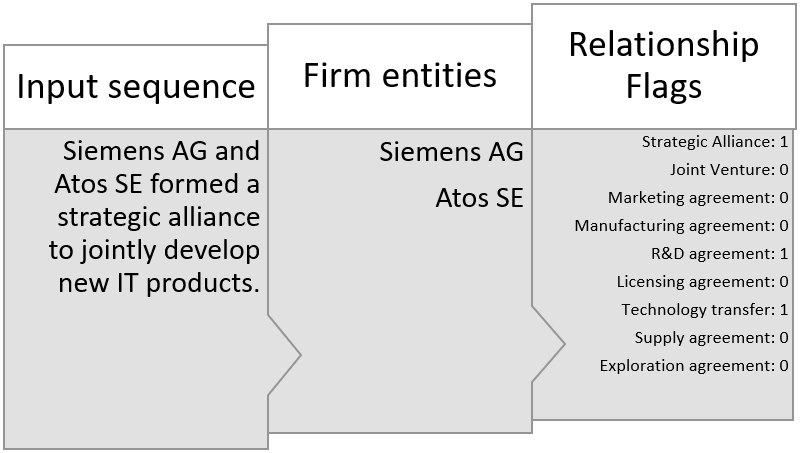
\includegraphics[width=0.7\textwidth]{./Figures/problem_statement.png} 
%\caption{Problem statement.}
%\label{fig:problem}
%\end{figure}

%%%%%%%%%%%%%%%%%%%%%%%%%%%%%%%%%%%%
\subsubsection{Firm name recognition} 
%%%%%%%%%%%%%%%%%%%%%%%%%%%%%%%%%%%%
In order to detect firm names, we use the Spacy transformer NER pipeline \citep{spacy2}. The pipeline has state of the art performance and is much less computationally burdensome than other systems. The pipeline was trained on a manually annotated dataset to distinguish various types of entities, including organization names.\footnote{According to the definition at \url{https://schema.org/Organization}.} This is a supercategory to firms/corporation, however, we can simply filter out organizations that cannot be matched to a firm database. This also allows the model to extract university-industry collaborations (these are also present in the knowledge base), which might be of interest to some researchers. When applying the pipeline to the LexisNexis articles, we combine the organizations detected by the model with the company tags supplied by LexisNexis, and retain only those names that can be matched to a firm in the Orbis database.
The more difficult problem is that of classifying the input sequence - identifying relevant sequences and then giving them the appropriate flags. We will discuss solutions to this problem below.

%%%%%%%%%%%%%%%%%%%%%%%%%%%%%%%%%%%%
\subsubsection{Representations from deep neural networks and transfer learning}
%%%%%%%%%%%%%%%%%%%%%%%%%%%%%%%%%%%%
There are a number of ways in which we could set up a model to extract and flag relations: For instance, we could come up with a set of rules (e.g. keywords occurring in a certain order) that would determine how a sequence is classified. This approach (called symbolic Natural Language Processing) usually falls short because of the high degree of variation in natural language and quickly becomes very complex, especially in a multi-label setting like ours. \\\\
A more modern approach is to construct representations of words in a vector space that try to capture its semantic properties in the given context. Given these vectors, we can then train a classifier (such as logistic regression or support vector machines). Naturally, the question is how to construct representations that are useful for downstream tasks. In the past, manually engineered vectors (e.g. binary indicators for whether a word co-occurs with a certain other word or is negated) or statistical embeddings (e.g. TF-IDF) have been used. \\\\
Since the 2010s, representations learned from deep neural networks have become the dominant methodology as they tend to perform substantially better. Commonly used language models now have hundreds of millions of parameters, and large neural networks require large amounts of training data. One important paradigm that has emerged because of that \textit{transfer learning}. Language models like BERT, GPT, or XLM are pre-trained on massive amounts of raw text data (such as the Common Crawl web crawl corpus) on a task like next word prediction. The resulting model can then be used for supervised downstream tasks like sequence classification or question answering, either by taking the hidden states of the neural network as a direct input for another classifier or by adding a task-specific output layer and fine-tuning the neural network using the given labels. The pre-trained model therefore serves as very useful initialization of the network, that appears to contain a lot of knowledge about the semantics of a language. Compared to pre-training, which requires substantial computational resources (and produces emissions comparable to those of a transatlantic flight, see \citet{strubell2019energy}), fine-tuning is relatively inexpensive and can be done on a single GPU.

%%%%%%%%%%%%%%%%%%%%%%%%%%%%%%%%%%%%
\subsubsection{The transformer architecture and BERT}
%%%%%%%%%%%%%%%%%%%%%%%%%%%%%%%%%%%%
Another important innovation has been the transformer architecture proposed by \citet{vaswani2017attention}. Recurrent architectures such as in Long Short Term Memory (LSTM) networks have the disadvantage of being computationally costly (their recurrent nature precludes parallelization). The transformer architecture solves this problem by feeding entire input sequences simultaneously into multiple layers of encoder and decoder blocks. Given our classification task, we are only concerned with the encoder blocks (the decoder serves to produce an output sequence, e.g. for translation). \\\\
First, since the words of input sequences are not fed to the model in order, we need to add positional encodings to input tokens. This is simply a number corresponding to the relative position of an input token in the sequence. Now, what happens in each encoder block? The inputs first go through a self-attention mechanism and then into a fully connected feedforward neural network. \\\\
Similar to how humans gain understanding by focusing on particular combinations  of words when reading a sentence (e.g. subject, verb, and object), the attention mechanism lets the network focus on a subset (in a fuzzy sense) of other input tokens when encoding each token. Using the attention patterns as input helps the neural network produce better context-dependent encodings. The transformer architecture uses scaled dot-product attention\footnote{It is worth noting that the time complexity of this type of self-attention scales quadratically with the sequence length $T$, so shorter input sequence are preferable.}:
\begin{gather*}
    A(Q,K,V) = softmax\bigg(\frac{QK^T}{\sqrt{d_k}}\bigg)V
\end{gather*}
where the query $Q$ is the current word that is operated on and $(K,V)$ is a set of learned key-value pairs. First, a similarity score of query and key is computed as $softmax(QK^T)$. Then it is multiplied with the stored values $V$. The division by $\sqrt{d_k}$ is simply a normalization to avoid vanishing gradients in the softmax ($d_k$ is the dimension of keys). The transformer architecture in fact employs multi-head attention, meaning that attention is computed multiple times in parallel with different learned matrices $K$ and $V$. The independent outputs from attention heads are then concatenated and projected into the desired dimension. This method of ensembling creates more useful and varied attention outputs. Figure \ref{fig:attention} shows the output of three attention heads (visualized with different colors) when queried with the word 'alliance' within the example sequence. The pink attention head makes the connection to the verb, while the orange head recognizes a connection to the word 'to', potentially allowing the model to make a connection to the purpose of the alliance. The blue head produces a less peaked output, connecting to the subjects, the verb, and the purpose of the alliance. The set of keys and values is learned like other parameters and varies between attention heads and layers. \\\\
The outputs of the self-attention layer for each position (each input token) are now each fed independently to a fully connected feed-forward neural network (FNN). The FNN applies two learned linear transformations with a rectified linear (ReLU) activation function in between:
\begin{gather*}
    FFN(x) = \max (0, xW_1 + b_1)W_2 + b_2
\end{gather*}
where the matrices $(W_1,W_2)$ and the vectors $(b_1,b_2)$ represent the learned weights and biases, respectively. These learned parameters vary from layer to layer. It is worth noting that each encoder block also employs residual connections between the self-attention and FNN sublayers, and finally applies layer normalization \citep{ba2016layer}, though we will not discuss these techniques in detail here. \\\\
The transformer was initially developed for sequence to sequence tasks (such as translation) but it turns out we can use the encoder part of the model to get useful representations for downstream tasks. This is exactly what BERT does: it builds \textbf{B}idirectional \textbf{E}ncoder \textbf{R}epresentations from \textbf{T}ransformers \citep{devlin2018bert}. \\\\
BERT$_{\text{large}}$ uses the transformer architecture with 24 encoder layers, each with 16 attention heads and 1024 neurons in the FFN. This makes for a total of 340 million parameters. The model is trained on two tasks, masked language modeling (randomly replacing a certain input token with [MASK] and letting the model predict the original input), and next sentence prediction (making the binary prediction whether a sentence follows another one). The pre-training corpora are the Books Corpus and English Wikipedia.
\begin{figure}[h!]
\centering
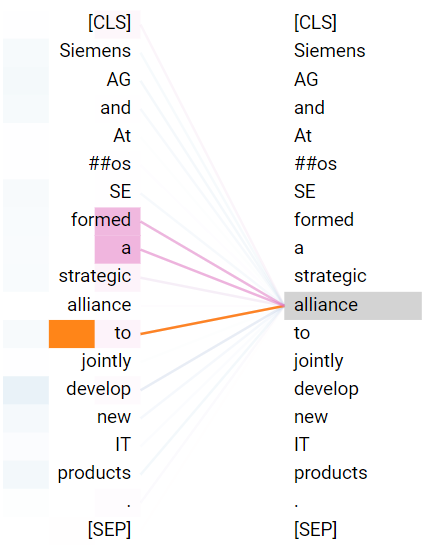
\includegraphics[width=0.5\textwidth]{./Figures/attention_demo.png} 
\caption{Visualization of the attention patterns produced by three attention heads in a BERT model. The patterns are at the 5th layer for the word 'alliance'. Visualization produced using \citet{vig2019transformervis}.}
\label{fig:attention}
\end{figure}

%%%%%%%%%%%%%%%%%%%%%%%%%%%%%%%%%%%%
\subsubsection{Tokenization and input embeddings}
%%%%%%%%%%%%%%%%%%%%%%%%%%%%%%%%%%%%
So far we have not discussed how words are fed into the encoder - after all, it takes as inputs vectors of real numbers and not a string sequence. A demonstration of how BERT generates input embeddings is given in figure \ref{fig:bert_token}. BERT uses WordPiece tokenization \citep{wu2016google} with a 30,000-word vocabulary. Essentially, it finds the 30,000 most common (sub-)words in the pre-training corpus and associates them with unique identifiers, which are then used as an input to the encoder. Out-of-vocabulary words are broken down greedily into sub-words that can be found in the vocabulary. As can be seen in the figure, the firm name 'Atos' is broken down into 'At', and '\#\#os', where the '\#\#' characters signify the continuation of a word. The BERT tokenizer also adds a [CLS] token to the beginning of each sequence, and a [SEP] token to separate sentences. The hidden states associated with the [CLS] token can be used for sequence classification tasks (they are representative for the whole sequence). The input layer of the neural network has a fixed size, so all inputs need to have the same length $T$. We, therefore, add a [PAD] token to bring shorter sequences to the desired length (these tokens are given 0 weight by an attention mask so they do not affect results). Longer sequences will simply be truncated at the maximum input length.
\begin{figure}[h!]
\centering
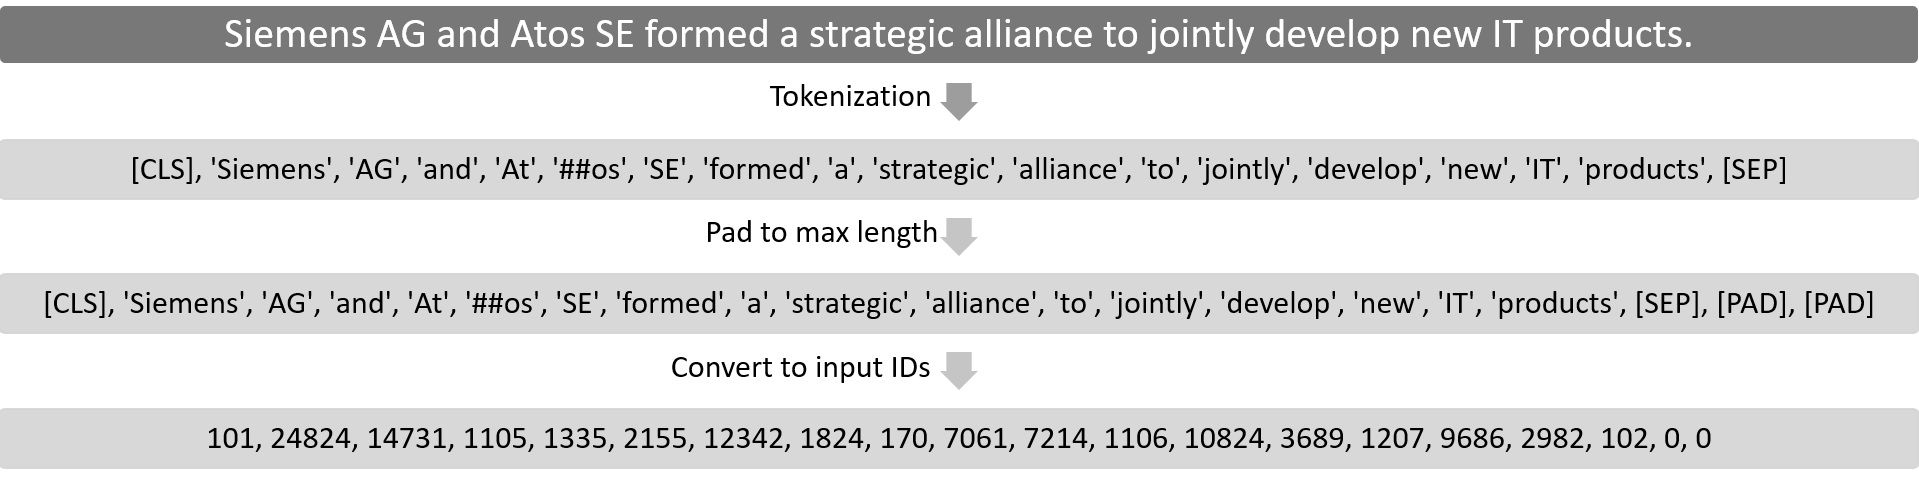
\includegraphics[width=\textwidth]{./Figures/BERT_tokenization_demonstration.jpg} 
\caption{How BERT creates input representations.}
\label{fig:bert_token}
\end{figure}

%%%%%%%%%%%%%%%%%%%%%%%%%%%%%%%%%%%%
\subsubsection{Details, output layer, and loss}
%%%%%%%%%%%%%%%%%%%%%%%%%%%%%%%%%%%%
In practice, we will make use of the LUKE model \citep{yamada2020luke}, which builds on Facebook's RoBERTa model \citep{liu2019roberta}. RoBERTa is architecturally the same as BERT$_{\text{large}}$, but is shown to improve on BERT in almost all downstream tasks by using longer pre-training with bigger batches, simplified training strategies (only masked language modeling), and a better set of hyperparameters. It is also trained on a larger set of corpora, importantly for us including the Common Crawl News dataset \citep{nagel2016cc}. The fact that the model has been pre-trained on a large news dataset likely leads to better performance in our downstream task in the same domain, with similar documents. Note that RoBERTa uses the BPE tokenizer \citep{sennrich2015neural} with a larger vocabulary that we will not discuss in detail here. LUKE augments this architecture with entity embeddings and entity-aware self-attention: the two candidate firm names are marked in the input sequence, and the relation labels are predicted for that pair of entities. \\\\
We use \textit{alliance} and \textit{collaborative agreement} interchangeably to mean any cooperative arrangement between two or more firms that the SDC database records as either a strategic alliance or a joint venture. Each alliance is described along three dimensions: its governance form (joint venture or strategic alliance---mutually exclusive), its status (planned, completed, or terminated), and its purpose. The purpose flags---marketing, manufacturing, R\&D, licensing, supply, exploration, and technology transfer---are not mutually exclusive, since a single alliance may serve several purposes at once. \\\\
Let us now discuss the output layer we need to add to the RoBERTa model for our multi-label classification task. We decide to include 10 labels in the analysis: whether an agreement is a Joint Venture or Strategic Alliance, whether the agreement is completed/signed or planned, and 6 flags for the type/purpose of the agreement: marketing, manufacturing, R\&D, licensing, supply\footnote{Note that the supply flag in the SDC data does not identify the direction of a buyer-supplier relationship.}, and exploration (these flags are not mutually exclusive). We also try to predict whether a technology transfer takes place (which is also not mutually exclusive with any other labels). The final label is simply whether a given sequence is relevant - in the sense of containing an alliance announcement. \\\\
Since we have 10 labels, we need 10 neurons in the output layer, each taking inputs of size 1024 (the size of the last hidden layer of RoBERTa associated with classifier token [CLS]), and producing output of size 1. Since we want non-exclusive outputs, we take a sigmoid activation function for each neuron:
\begin{gather*}
    \hat{p}(y_i)=\sigma(z_i)=\frac{1}{1+e^{-z_i}},
\end{gather*}
where $\hat{p}(y_i)$ is the predicted probability for class $i$ and $z_i$ is the output of neuron $i$. This setup means we can output probabilities for all classes independently from each other. We also need an appropriate loss function. Since we already take the sigmoid activation function in the output layer, we use a weighted binary cross-entropy loss, which for a given example is:
\begin{gather*}
    L(\hat{p}(y),y) = - \sum_{i=1}^{C} w_i \big( y_i \log(\hat{p}(y_i)) + (1-y_i) \log(1-\hat{p}(y_i)) \big)
\end{gather*}
where $y$ is the vector of ground-truth labels for that example, $w_i$ is the weight of label $i$, and $C$ is the number of labels. This function computes the loss for each element in $y$ (each class) independently. With the label weights, we can adjust how much emphasis is put on getting correct predictions for each label. In practice, we will use them to make up for the class imbalance in the dataset. We want to predict all labels equally well, so we calculate label weights as
\begin{gather*}
    w_i = \frac{1}{2 \text{SP}_i},
\end{gather*}
where $\text{SP}_i$ is the share of examples in the training set that is labeled positively for label $i$. This means that a label with an equal number of positive and negative examples receives weight 1, while a label with only one-quarter of examples being positive would receive weight 2. \\\\
For training the model, we take a batch size of 64 and fine-tune over 2 epochs over the data. We set the maximum sequence length to $T=64$ tokens. This is enough to accommodate almost all examples in full length (and in the cases where the sequence is cut off the tokens at the end would likely not be important for classification). We use the Adam optimizer \citep{kingma2014adam} with a learning rate of $5e^{-5}$, $\beta_1=0.9$, $\beta_2=0.999$, and $\epsilon=10^{-8}$, as \citet{devlin2018bert} used for fine-tuning BERT. The model was trained on a single Tesla T4 in 6 hours using 16-bit floating-point precision.
% To prevent the model from overfitting on firm names, we replace detected firm names with the '[MASK]' token used in the BERT masked language modeling task.
% Since we have a multi-label classification

%%%%%%%%%%%%%%%%%%%%%%%%%%%%%%%%%%%%
\subsection{Knowledge Base and Training Data}
\label{sec:knowledge_base} 
%%%%%%%%%%%%%%%%%%%%%%%%%%%%%%%%%%%%
We use a knowledge base of alliances, which provides positive examples to train and evaluate our model on. We also use a training corpus of news articles, which is used to generate negative examples for the training set. Inference is then run on the separate collection of LexisNexis articles described in Appendix \ref{sec:lexis_search}.

%%%%%%%%%%%%%%%%%%%%%%%%%%%%%%%%%%%%
\subsubsection{Knowledge base}
%%%%%%%%%%%%%%%%%%%%%%%%%%%%%%%%%%%%
We use the Refinitiv (formerly Thomson Financial) SDC Platinum Joint Venture (JV)/Strategic Alliance (SA) database as our knowledge base. The database has a wide coverage of worldwide inter-firm relations: It collects JV/SA transactions from newspapers, trade journals, government filings, and newswires. It features a little over 196,000 entries in the period from 1985 to the present. The distribution of these entries along time, countries, and industries is given in Figure \ref{fig:dealdist}, along with the number of participants per deal. The number of deals per year varies quite significantly, with a noticeable drop in entries between the years 2009 and 2016. Given that the data is incomplete, we cannot evaluate whether this is a real-world trend or is due to a change in methodology. The overwhelming majority of participants is headquartered in the United States. The data covers a wide range of industries and does not appear to have the strong bias towards particular industries that other alliance databases have. The number of participants is typically between two and four. The data does have some missing participant names, with zero or only one recorded participants (clearly an alliance takes at least two participants). Our firm name recognition system can be used to fill in these missing names. \\\\
\begin{figure}[h!]
\centering
\begin{subfigure}[t]{0.45\textwidth}
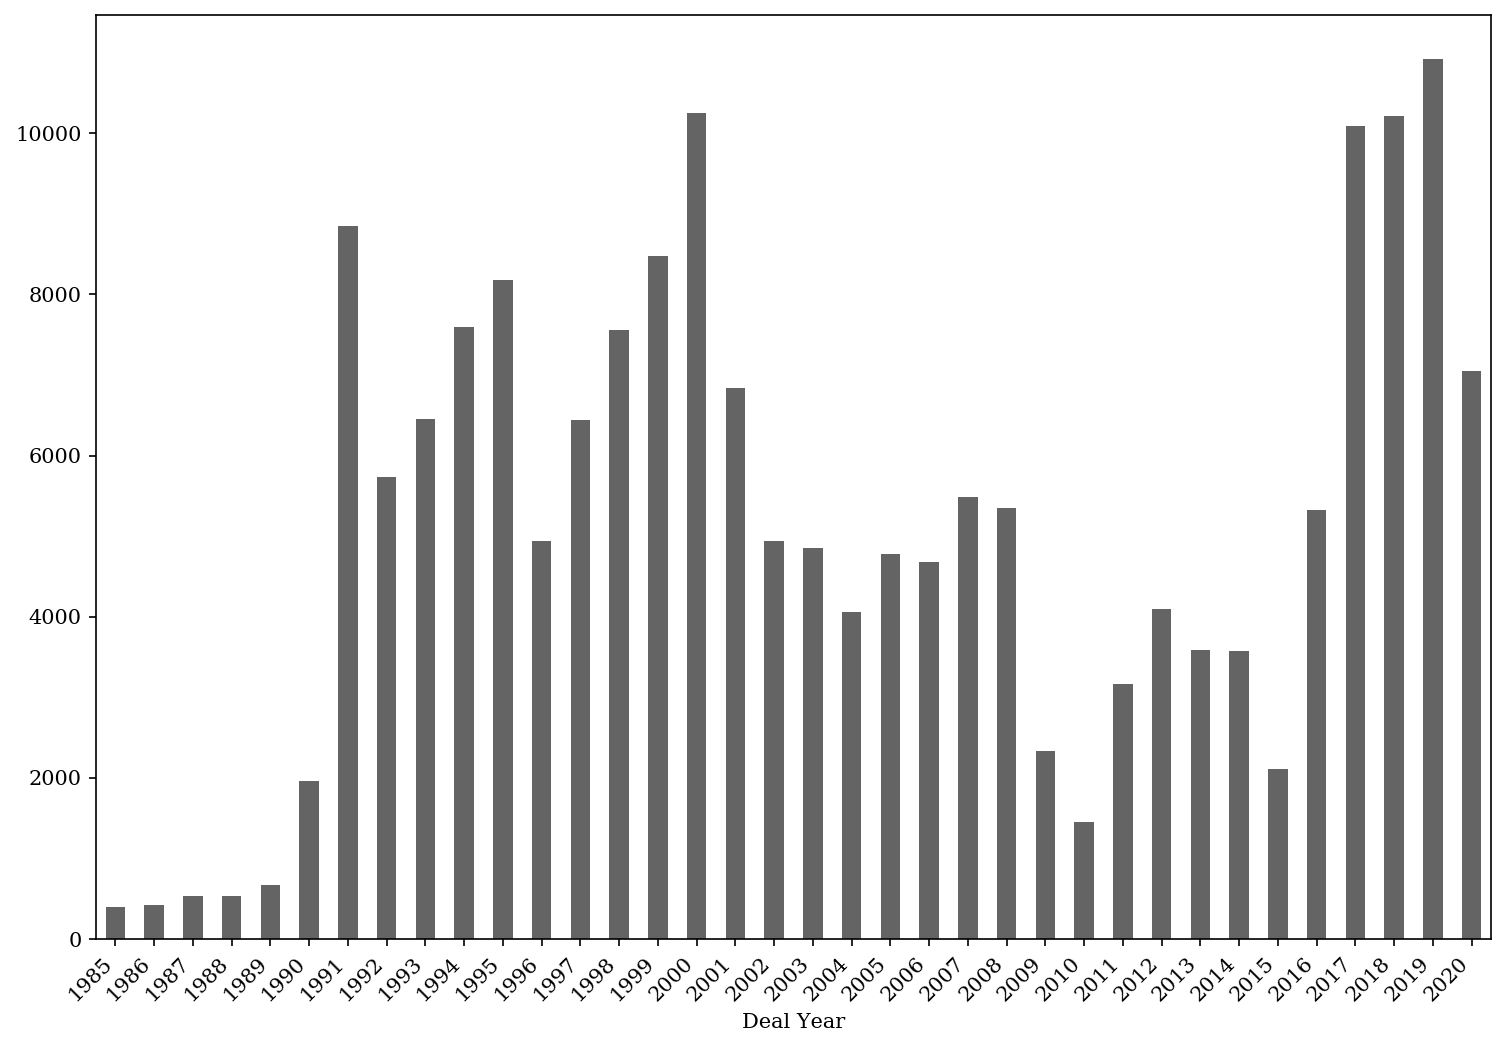
\includegraphics[width=\textwidth]{./Figures/dealsovertime_gray.png} 
\caption{Deals over time.}
\end{subfigure}
\begin{subfigure}[t]{0.45\textwidth}
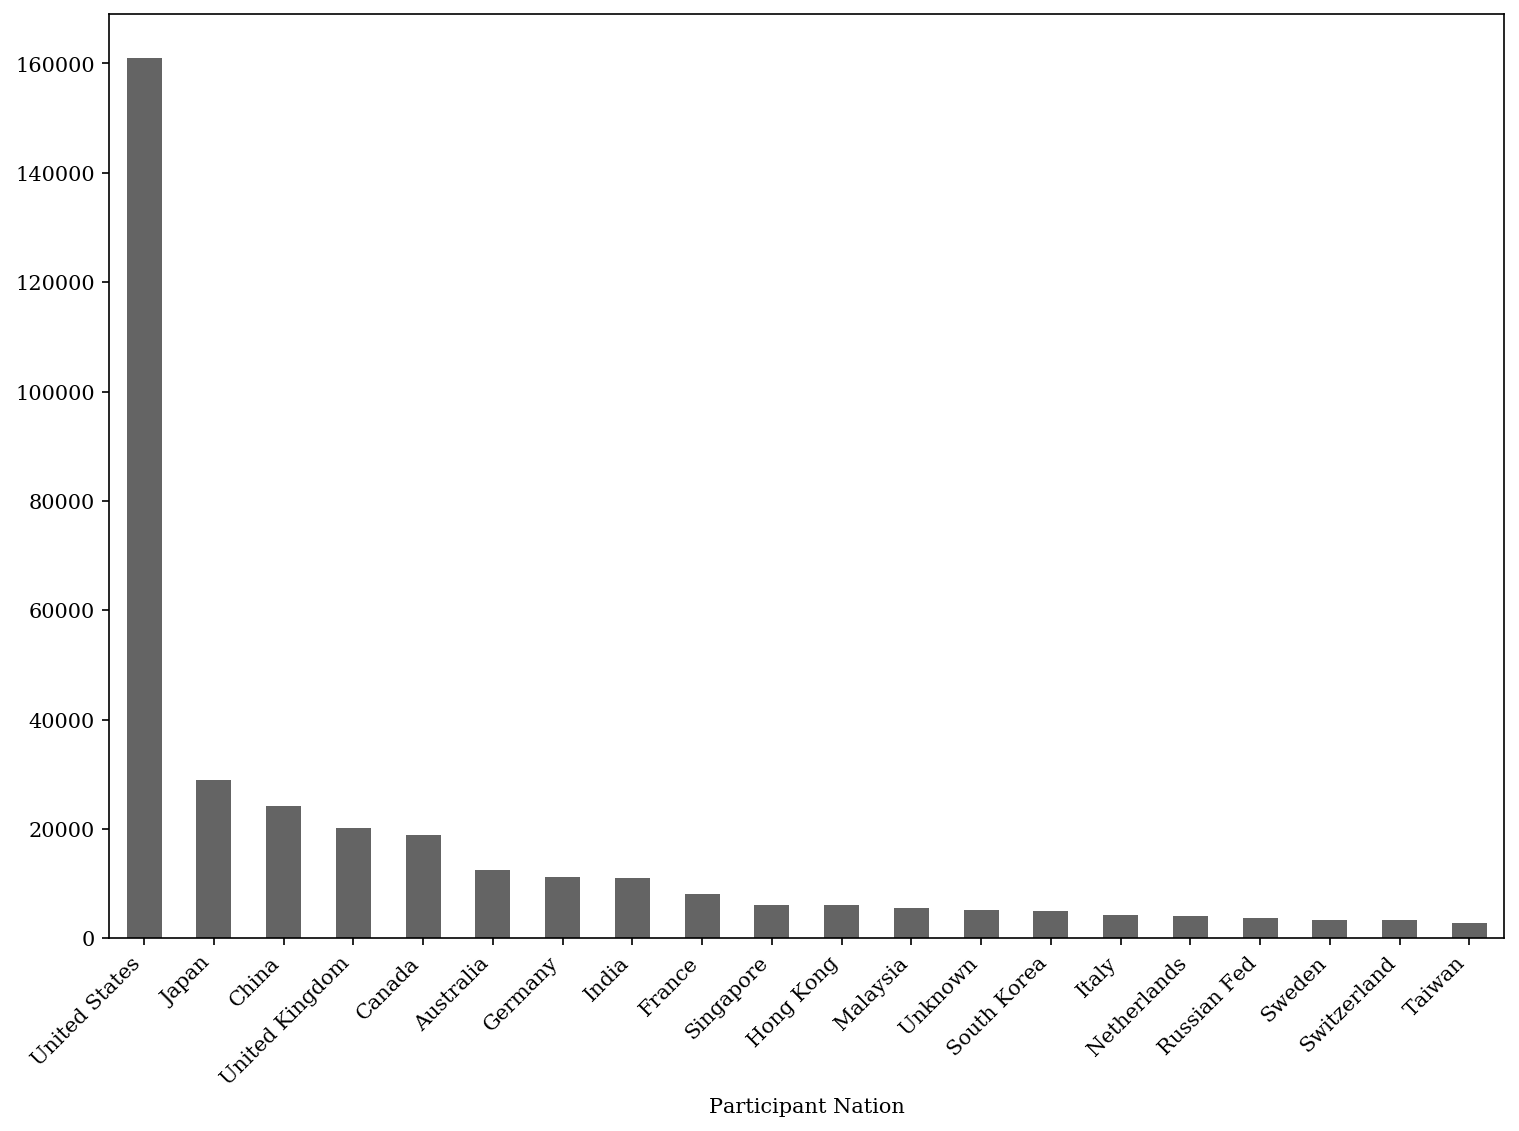
\includegraphics[width=\textwidth]{./Figures/PartCountries_gray.png} 
\caption{Top 20 participant countries.}
\end{subfigure}
\begin{subfigure}[t]{0.45\textwidth}
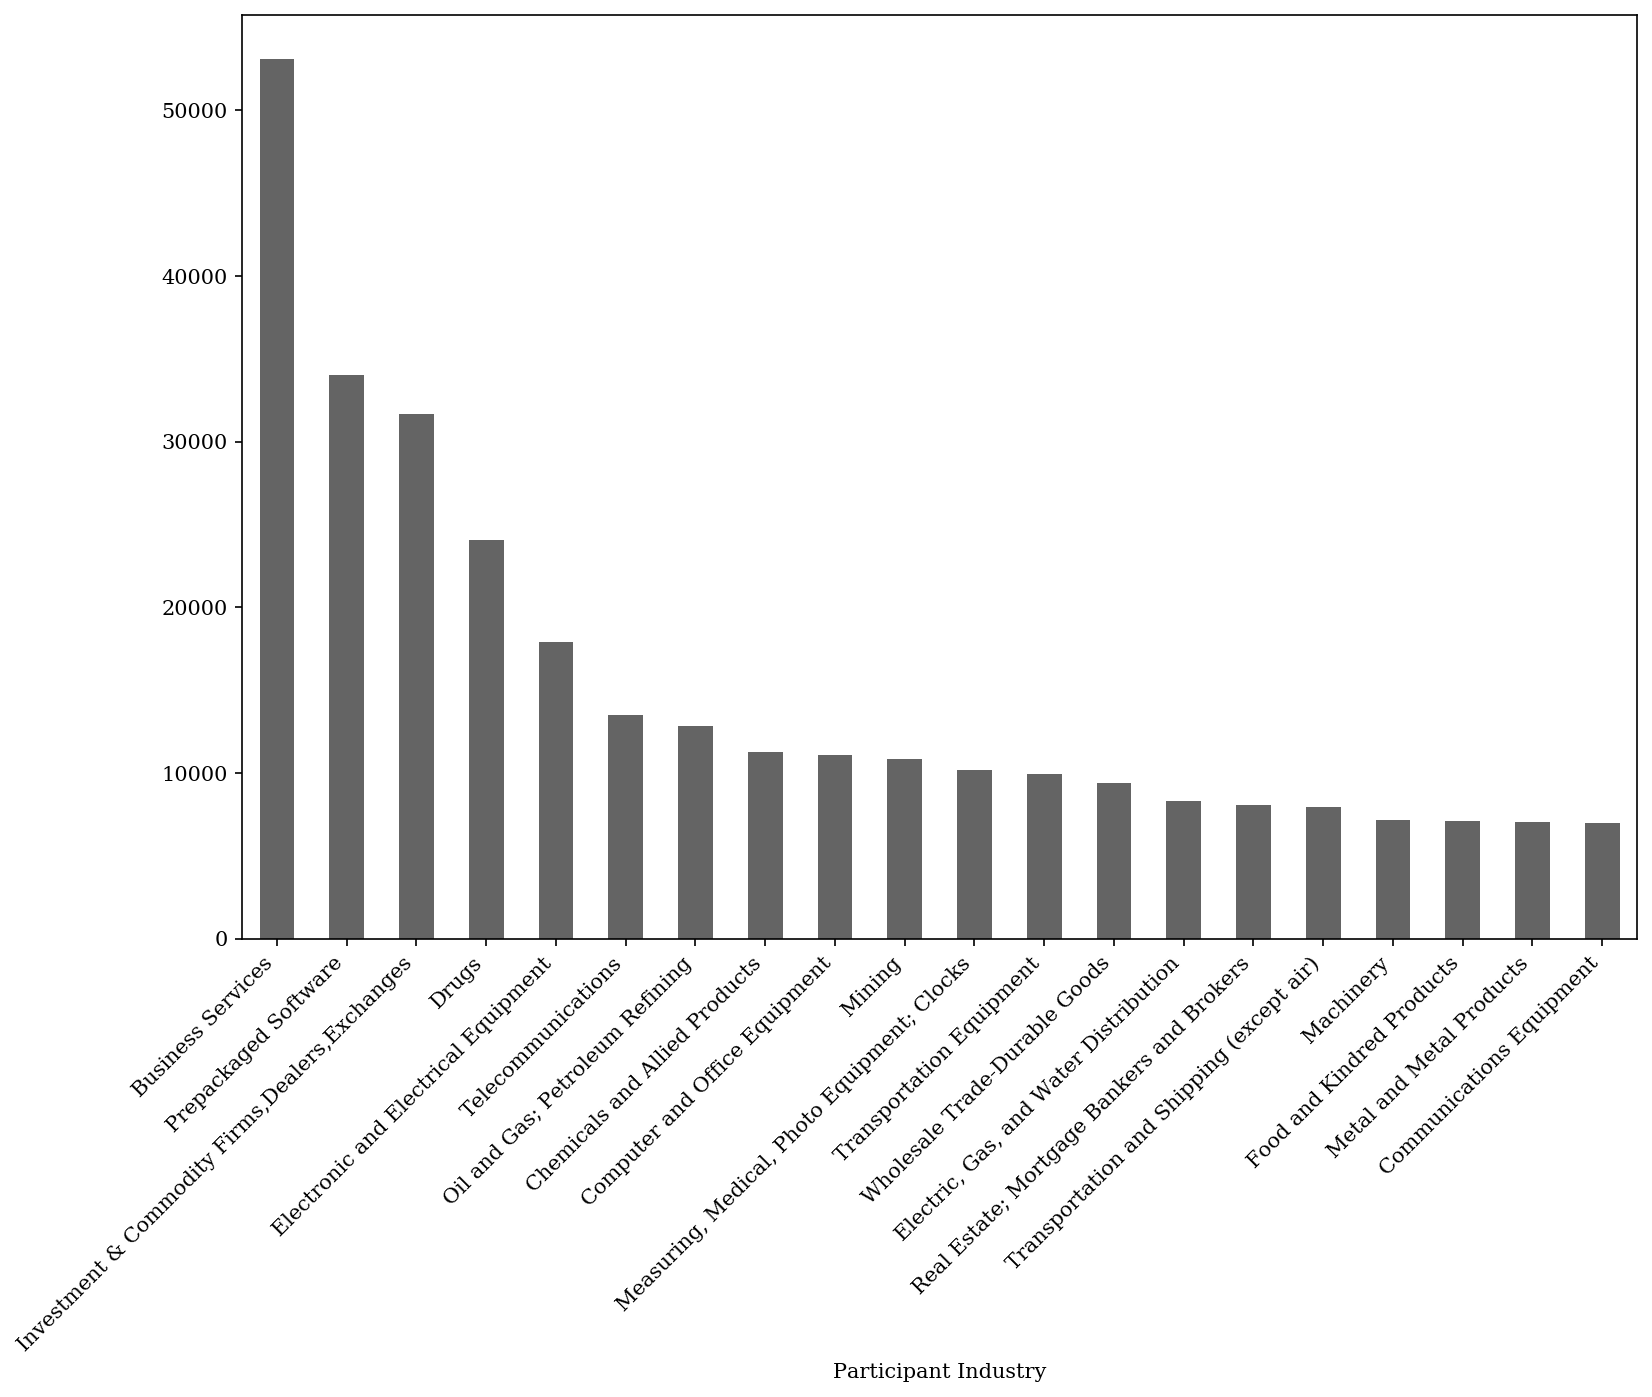
\includegraphics[width=\textwidth]{./Figures/PartIndustries_gray.png} 
\caption{Top 20 participant industries.}
\end{subfigure}
\begin{subfigure}[t]{0.45\textwidth}
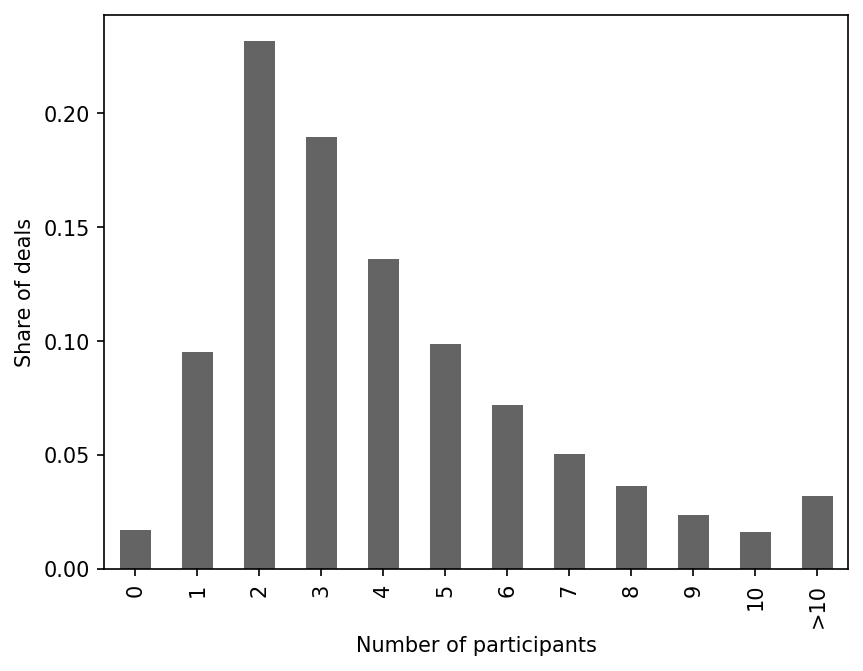
\includegraphics[width=\textwidth]{./Figures/PartDist_gray.png} 
\caption{Number of participants per deal.}
\end{subfigure}
\caption{Distribution of deals in the SDC Platinum JV/SA database.}
\label{fig:dealdist}
\end{figure}
\noindent According to Refinitiv, the data is created by content analysts manually evaluating each source document. Since the database also features the original 'deal text' that an entry is based on, it represents a rich source of manually labeled examples that can be used to teach information extraction algorithms. \\\\
We narrow down our sample according to several criteria. First, we drop observations with missing deal text, missing flags for the type of deal, or clearly erroneous entries. We then focus on deals with a ?completed/signed?, "pending", or "terminated" status. There are only a few entries that do not fall into these categories; we remove them to populate our test set only with examples of 'positive' developments, i.e. an agreement being reached rather than reviewed. We retain the terminated agreements and predict the terminated status as a separate label, rather than using them as negative examples. As to why we do not remove "pending" observations, a typical deal text for entries with "pending" status is given below:
\begin{displayquote}
\small{\textit{"Redcargo Logistics and GD Express Carrier Bhd planned to form a strategic alliance.The purpose of the strategic alliance is to provide GDEX customers with access to AirAsias extensive network, meaning goods are able to be transported and delivered efficiently on more than 5,000 weekly flights across Asia Pacific."}}
\end{displayquote}
The original source only mentions the agreement is "planned". Unfortunately, these entries are not typically updated after an agreement is actually signed. In many cases, it is easily verified using a search engine that these agreements came into effect at one point. Not considering these entries would therefore mean missing a lot of developments (about 44\% of entries have "pending" as status). We simply take the pending/completed distinction as another variable to be predicted. This also means that our system can improve upon the existing data by updating agreements from planned to signed once this is confirmed in a news article. \\\\
There are 16 flags in the dataset that describe the kind of relation stated in the source document. Every entry is first categorized as a strategic alliance or joint venture. Then there are a number of flags that describe the purpose of the agreement, e.g. manufacturing or marketing. We are only interested in the most common types of relations and exclude several categories that are empirically rare from our analysis. We combine the flags "Licensing Agreement",  "Exclusive Licensing Agreement", and "Cross-Licensing Agreement" into a common licensing category, as well as combining "Technology Transfer" and "Cross-Technology Transfer" (it is often unclear from the deal text whether there is technology transfer in both directions; the distinction between the two labels seems to be assigned relatively arbitrary). The number of occurrences and co-occurrences for each flag is given in Figure \ref{fig:co_occ}. The SA/JC and pending/completed classification are mutually exclusive, all other labels have some overlap. The latter is empirically plausible, as a deal might for instance include both a manufacturing and R\&D component. This makes this a multi-label classification problem. To account for the fact that SA/JC and pending/completed are mutually exclusive categories, we choose label encoding for these variables and one-hot encoding for the other flags. This transforms the problem into a multi-label binary classification problem. The corresponding neurons in the output layer are therefore tasked to classify a deal text as JV or SA, pending or completed, licensing agreement or not, manufacturing agreement or not, etc. \\\\
\begin{figure}[h!]
\centering
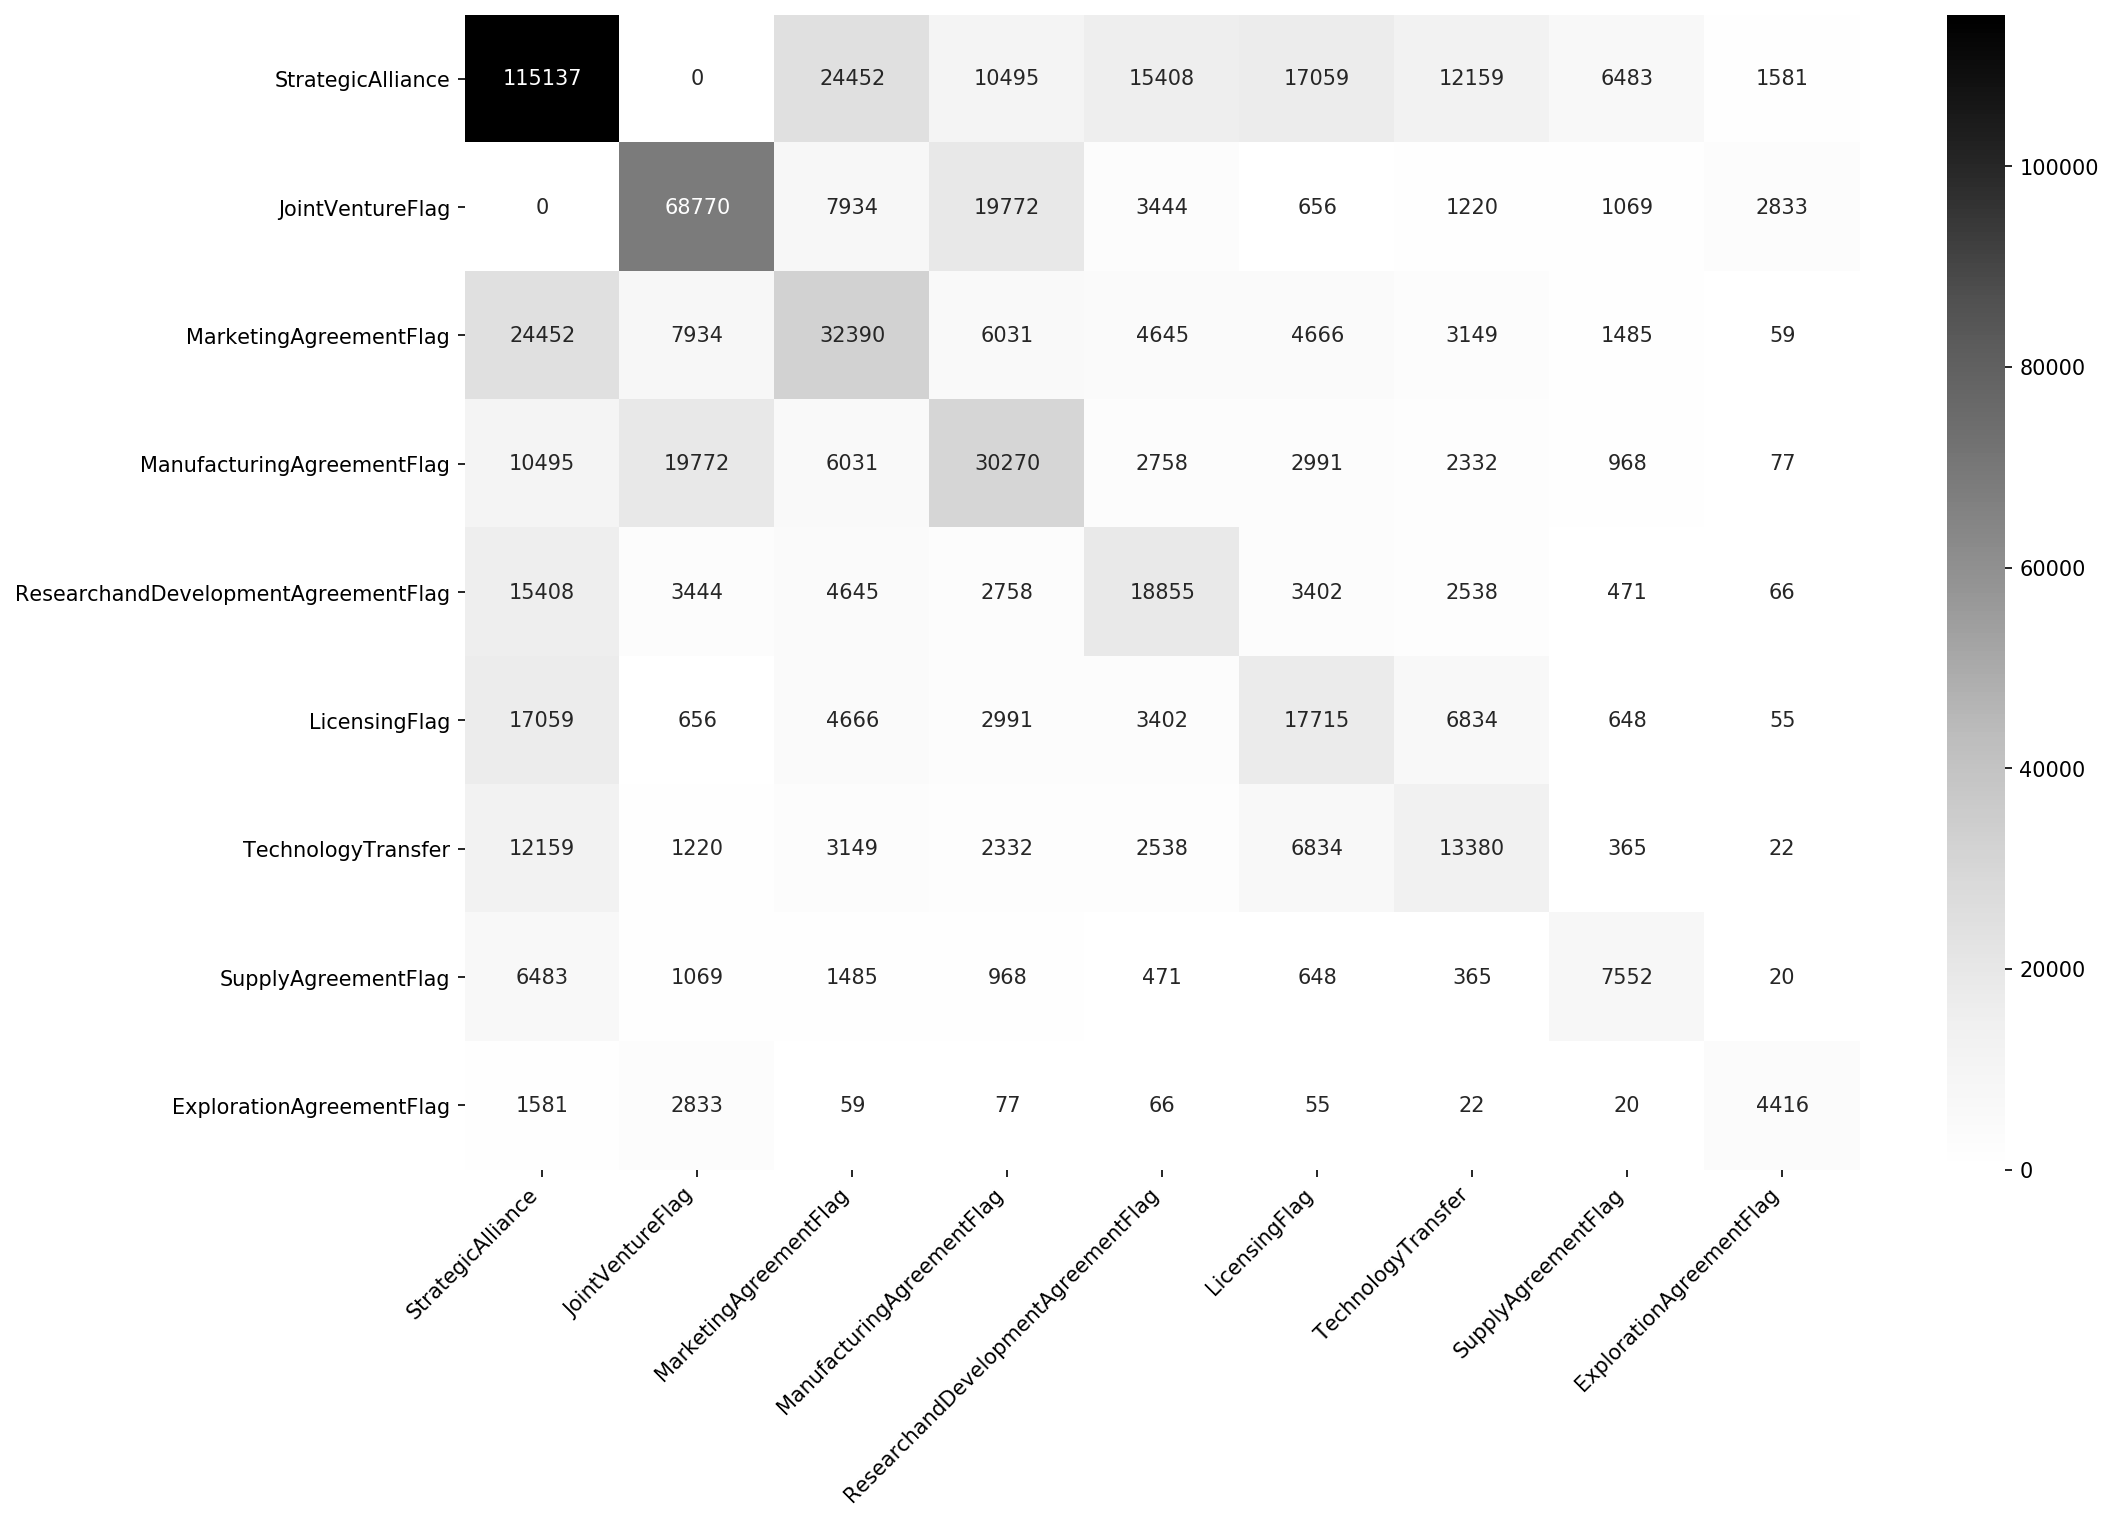
\includegraphics[width=\textwidth]{./Figures/co_occur.png} 
\caption{Ocurrences and co-occurences of relationship labels in the SDC Platinum JV/SA database.}
\label{fig:co_occ}
\end{figure}

%%%%%%%%%%%%%%%%%%%%%%%%%%%%%%%%%%%%
\subsubsection{Training corpus}
%%%%%%%%%%%%%%%%%%%%%%%%%%%%%%%%%%%%
The corpus from which we draw negative examples is a collection of financial news articles from Bloomberg and Reuters between October 2006 to November 2013. The collection was released by \citet{ding2014using}. It is used only for training and is disjoint from the LexisNexis collection on which we later run inference. After removing articles with missing dates, and empty or scrambled bodies of text, we are left with a total of 421,387 news articles. Most articles date to the years 2010 to 2013 and three-quarters of articles are sourced from Bloomberg (the remaining articles are from Reuters). The average length of each article is 525 words (including the headline). Few articles only have a headline; most fall somewhere between 100 and 1000 words. Since we have to choose a maximum sequence length to feed into our model (e.g. 128 tokens), we would have to split longer documents into smaller chunks of that length with some overlap as not to lose the context. We choose not to do this for inference and instead just parse the beginning of each document. This is because we want to focus on articles where a given deal is the main piece of news reported, not articles that mention an old deal as background information somewhere deep in the body of the text. First, this makes it much more plausible to take the date of the article as the date of the inception of the deal. Second, such articles will provide a better and more succinct description of the deal.

%%%%%%%%%%%%%%%%%%%%%%%%%%%%%%%%%%%%
\subsubsection{Constructing a training set}
%%%%%%%%%%%%%%%%%%%%%%%%%%%%%%%%%%%%
We want the model to be able to first detect if a document/sequence is relevant and then give it the appropriate flags. To detect if a document is relevant (in the sense of mentioning a collaborative deal between two or more firms) we add another outcome variable, where all examples from the knowledge base are labeled positive. Negative examples are drawn from a disjoint set of documents: articles in the Bloomberg/Reuters corpus that contain no alliance announcement. We first discard any article matching a list of 34 collaboration-related keyword patterns anywhere in its body (e.g. "joint venture", "strategic alliance", "licensing agreement", "agreed to jointly develop"), so that articles reporting an alliance in any paragraph are excluded entirely. From each remaining article we drop the headline and retain the first $k$ sentences, where $k$ is drawn from the empirical distribution of sentence counts in SDC deal texts, so that negatives match positives in length and structure. We then require the retained text to mention at least two distinct organizations that match a firm name in Orbis within the first 800 characters, and mark the first two as the candidate entity pair with an empty relation label. This entity requirement ensures the model cannot separate the classes simply by detecting the presence of two firm names, and must instead learn whether a collaborative relationship is asserted between them. We sample negatives until the training set is balanced 1:1. \\\\
Alliance entries with status 'terminated' are not used as negative examples. Instead, we keep them as positive examples and add the terminated status as a separate label, so that the model learns to recognize mentions of deal terminations rather than treating them as irrelevant text. \\\\
We have 359,622 total examples, of which half are negative and half are positive. We use a train-test split of 2:1 since we have plenty of training data and a large test set allows us to get a more accurate estimate of model performance. We do not bother with making a stratified train-test split. Considering the number of examples in relation to the class distribution (compare Figure \ref{fig:co_occ}) we get a very even split by the law of large numbers (we verified this to be true for our particular split).

%%%%%%%%%%%%%%%%%%%%%%%%%%%%%%%%%%%%
\subsection{Model performance}
\label{sec:performance} 
%%%%%%%%%%%%%%%%%%%%%%%%%%%%%%%%%%%%
In the following, we evaluate the pipeline on firm name recognition, relation classification, and finally the quality of inference on previously unseen articles from the corpus.

%%%%%%%%%%%%%%%%%%%%%%%%%%%%%%%%%%%%
\subsubsection{Firm name recognition}
%%%%%%%%%%%%%%%%%%%%%%%%%%%%%%%%%%%%
First, we want to check how accurately our NER system detects the firm names mentioned in deal texts. For each deal in the knowledge base, we compare the set of recorded participants $A$ with the set of organizations recognized by the algorithm $B$. We compute the share of recognized participants as 
\begin{gather*}
    S(A,B) = \frac{|A \cap B|}{|A|},
\end{gather*}
meaning that we give partial credit for recognizing some of the participants.
% We also determine when all participants in $A$ are recognized by the algorithm:
% \begin{gather*}
%     \text{all\_recognized}(A,B) = \mathbbm{1}_{|A \cap B|=|A|}
% \end{gather*}
We then simply average this score over all deals in the knowledge base. The Spacy model was trained on completely unrelated data so we can use the full knowledge base as a test set, to check whether the model works well for this application. To check whether individual recognized firm names are the same, we strip the names from both $A$ and $B$ of all legal business type identifiers (such as "Co.", Inc.", and "Ltd"). We take the full list of legal identifiers from \citet{schwenkler2019network}, who also use it to solve the problem of firm name matching. \\\\
The average share of recognized participants in the full knowledge base is an excellent 89.2 percent. Note that about 10 percent of entries in the knowledge base have zero or only one recorded participant. These entries were excluded from calculating the score because they are clearly incomplete (for these cases the firm name recognition algorithm can also help to fill in the missing participant names).

%%%%%%%%%%%%%%%%%%%%%%%%%%%%%%%%%%%%
\subsubsection{Relationship classification}
%%%%%%%%%%%%%%%%%%%%%%%%%%%%%%%%%%%%
Next, we need to evaluate the performance of our model in the relation classification task. We will look at precision (true positives as a share of true positives plus false positives), recall (true positives as a share of true positives plus false negatives), the F1-measure (the harmonic mean of precision and recall), as well as accuracy (the share of correct predictions). We do this for each label individually, but we also look at the Macro score subset accuracy, which is the share of examples where the predictions exactly match the set of \textit{all} labels. Note that the alliance flags only make sense if an alliance is mentioned. We, therefore, evaluate the accuracy for these labels only on knowledge base examples, as not to inflate the accuracy scores (it does not make a difference for the other scores). \\\\
Macro average gives greather emphasis to rare labels
The performance metrics are given in Table \ref{tab:performance}. The model achieves great precision and recall on finding relevant sequences with alliance agreements, distinguishing pending from completed agreements and joint ventures from strategic alliances. It also does fairly well on assigning the manufacturing and licensing agreement flags, and a little bit worse on the R\&D, marketing, and exploration agreement flags. The model is not able to predict the supply agreement and technology transfer agreement flags well. This can be caused both by the limited number of positive examples for these labels, as well as labels that do not follow a clear decision rule. When inspecting the original deal text along with the supply agreement and technology transfer labels it becomes clear that these are relatively subjective codings with reliability issues. The supply agreement flag seems to have been applied The system also achieves a subset accuracy of 89.1 percent. The relatively poor performance on the technology transfer and supply agreement labels does not affect this score much because these examples are relatively uncommon.
\begin{table}[]
    \centering
    \begin{tabular}{lllll}
    \toprule
    {} & Precision &    Recall &  F1-score &  Accuracy \\
    \midrule
    Relevant                &  0.989 &  0.971 &  0.980 &  0.981 \\
    Pending                 &  0.938 &  0.964 &  0.951 &  0.970 \\
    Joint Venture           &  0.983 &  0.990 &  0.987 &  0.990 \\
    Strategic Alliance      &  0.994 &  0.990 &  0.992 &  0.990 \\
    Marketing agreement     &  0.864 &  0.739 &  0.797 &  0.933 \\
    Manufacturing agreement &  0.878 &  0.830 &  0.853 &  0.953 \\
    R\&D agreement           &  0.793 &  0.749 &  0.777 &  0.954 \\
    Licensing agreement     &    0.913 &   0.800 &  0.853 &  0.973 \\
    Supply agreement        &  0.674 &  0.461 &  0.548 &  0.969 \\
    Exploration agreement   &  0.776 &  0.764 &  0.770 &  0.990 \\
    Technology transfer     &  0.694 &  0.540 &  0.607 &  0.950 \\
    \bottomrule
    \end{tabular}
    \caption{Model performance on the relation classification task. The first row measures whether a sequence reports an alliance at all; the next rows measure its governance form and status; the remaining rows measure the purpose of the agreement and are not mutually exclusive.}
    \label{tab:performance}
\end{table}

%%%%%%%%%%%%%%%%%%%%%%%%%%%%%%%%%%%%
\subsubsection{Inference on the news corpus}
%%%%%%%%%%%%%%%%%%%%%%%%%%%%%%%%%%%%
Finally, we also want to get an idea of how well the model does in terms of inference on our news corpus. First off, the model is highly scalable: on one Tesla T4 GPU, we can do inference on roughly 150 documents per second. This means we can process millions of documents within a couple of hours. \\\\
An interesting question to ask is, for a given period of time, how many of the deals recorded in the knowledge base we can extract from our corpus. Naturally, this number is limited by the number of relevant documents in the corpus. Our corpus does not feature many of the primary sources used in the SDC data, such as business wires. Therefore we cannot expect to be able to extract a large share of deals from the knowledge base, but it is nevertheless good to see the amount of overlap between extracted alliances and alliances in the SDC data. We will take the year 2012 as a test for this since this is the year with most articles in our corpus. We take both knowledge base entries and negative examples from the corpus from 2012 out of the training set so this data has not been seen before by the model. \\\\
Out of 159,207 news articles in the year 2012, the model identified an alliance in 605 articles. Our aim in this exercise is to gauge coverage rather than precision: a precision estimate for this corpus would require manually comparing each extraction against its source article, which is beyond the scope of this evaluation. The overlap with the SDC data provides an external check instead. 112, or 18.5 percent of the extracted alliances can be found in the SDC data (we match entries if at least two of the participants are identical). Conversely, 2.7 percent of the 4156 alliances in the SDC data for this year are extracted from the corpus. As mentioned before, we would expect this share to rise with the quality and size of the analyzed corpus.

\FloatBarrier

%%%%%%%%%%%%%%%%%%%%%%%%%%%%%%%%%%%%%%%%%%%%%%%%%%%%%%%%%

%%%%%%%%%%%%%%%%%%%%%%%%%%%%%%%%%%%%%%%%%%%%%%%%%%%%%%%%%
\section{Additional Data Sources and Descriptives}
\label{sec:app-data}
%%%%%%%%%%%%%%%%%%%%%%%%%%%%%%%%%%%%%%%%%%%%%%%%%%%%%%%%%

%%%%%%%%%%%%%%%%%%%%%%%%%%%%%%%%%%%%%%%%%%%%%%%%%%%%%%%%%
\subsection{Network Characteristics}
\label{sec:net-char}
%%%%%%%%%%%%%%%%%%%%%%%%%%%%%%%%%%%%%%%%%%%%%%%%%%%%%%%%%
The total number of firms in our sample is 15,103. Tables  \ref{tab:1990_deg_ranking-nace}, \ref{tab:2000_deg_ranking-nace},  \ref{tab:2010_deg_ranking-nace} and  \ref{tab:2020_deg_ranking-nace} show the 25 highest ranked firms according to their degree (i.e. the number of collaborations) in the year 1990, 2000, 2010 and 2020, respectively. From these tables we observe that the rankings are highly unstable, with the highest ranked firms changing across the years considered. This could be due to the changing importance of different sectors in terms of the R\&D collaboration intensity as illustrated in Figure \ref{fig:top5-industries}.

%Table \ref{tab:1990_deg_ranking-nace} shows the 25 highest ranked firms according to their degree (i.e. the number of collaborations) in the year 1990. 	
\begin{table}[tbp]
\vspace{-2cm}
\centering
\scalebox{0.75}{
\begin{sideways}
\begin{threeparttable}
  \centering
  \caption{The 25 highest ranked firms according to their degree (i.e. the number of collaborations) in the year 1990.}
     \begin{tabular}{lrrrr}
    \toprule
Name & Deg. & NACE & NACE Description & Rank \\ 
    \midrule
Eastman Kodak Co & 15&   26 & Manufacture of computer, electronic and optical products & 1 \\ 
Du Pont Limited & 14&   20 & Manufacture of chemicals and chemical products & 2 \\ 
General Electric Company & 14&   30 & Manufacture of other transport equipment & 3 \\ 
Sun Limited & 11&   55 & Accommodation & 4 \\ 
Ciba - Geigy & 10&   20 & Manufacture of chemicals and chemical products & 5 \\ 
AT\&T Inc. & 10&   61 & Telecommunications & 6 \\ 
Texas Instruments Inc & 10&   26 & Manufacture of computer, electronic and optical products & 7 \\ 
Sun Microsystems (south Africa) (pty) Ltd & 10&   58 & Publishing activities & 8 \\ 
Philips Gmbh & 9&   64 & Financial service activities, except insurance and pension funding & 9 \\ 
Kodak Limited & 9&   58 & Publishing activities & 10 \\ 
Mitsubishi Corp. & 9&   46 & Wholesale trade, except of motor vehicles and motorcycles & 11 \\ 
Toshiba Corp. & 8&   26 & Manufacture of computer, electronic and optical products & 12 \\ 
Amoco & 8&   47 & Retail trade, except of motor vehicles and motorcycles & 13 \\ 
Olin Corp & 8&   20 & Manufacture of chemicals and chemical products & 14 \\ 
Tandem Computers Inc & 8&   46 & Wholesale trade, except of motor vehicles and motorcycles & 15 \\ 
Combustion Engineering & 8&   35 & Electricity, gas, steam and air conditioning supply & 16 \\ 
Monsanto Co & 8&   20 & Manufacture of chemicals and chemical products & 17 \\ 
Phillips Petroleum & 7&   61 & Telecommunications & 18 \\ 
Eos Holding Aktiengesellschaft & 7&   70 & Activities of head offices & 19 \\ 
Fujitsu Limited & 7&   26 & Manufacture of computer, electronic and optical products & 20 \\ 
Mobil & 7&   47 & Retail trade, except of motor vehicles and motorcycles & 21 \\ 
BASF Se & 6&   20 & Manufacture of chemicals and chemical products & 22 \\ 
Sumitomo Chemical Company Limited & 6&   20 & Manufacture of chemicals and chemical products & 23 \\ 
Computer Systems (private) Limited & 6&   62 & Computer programming, consultancy and related activities & 24 \\ 
Bass & 6&   22 & Manufacture of rubber and plastic products & 25 \\ 
%Chemical Industries (far East) Ltd & 6&   20 & Manufacture of chemicals and chemical products & 26 \\ 
%International Business Machines Corp & 6&   62 & Computer programming, consultancy and related activities & 27 \\ 
%ICI Llc & 6&   61 & Telecommunications & 28 \\ 
%Procter \& Gamble Co & 6&   20 & Manufacture of chemicals and chemical products & 29 \\ 
%Dow Chemical Company (the) & 6&   20 & Manufacture of chemicals and chemical products & 30 \\ 
\midrule
\bottomrule
    \end{tabular}%
        \begin{tablenotes}[flushleft]%
	\item \emph{Note:} The degree measures the number of R\&D collaborations of a firm. NACE refers to the current Statistical Classification of Economic Activities in the European Community (revision 2).
	\end{tablenotes}
  \label{tab:1990_deg_ranking-nace}
\end{threeparttable}
\end{sideways}
}
\end{table}

%Table \ref{tab:2000_deg_ranking-nace} shows the 25 highest ranked firms according to their degree (i.e. the number of collaborations) in the year 2000. 	
\begin{table}[tbp]
\vspace{-2cm}
\centering
\scalebox{0.75}{
\begin{sideways}
\begin{threeparttable}
  \centering
  \caption{The 25 highest ranked firms according to their degree (i.e. the number of collaborations) in the year 2000.}
    \begin{tabular}{lrrrrr}
    \toprule
Name & Deg. & Sales [\%] & NACE & NACE Description & Rank \\ 
    \midrule 
Microsoft Corporation & 75 & 1.6413 & 58 & Publishing activities & 1 \\ 
Siemens Ag & 61 & 0.0003 & 28 & Manufacture of machinery and equipment nec & 2 \\ 
Dupont & 48 & 0.0593 & 45 & Wholesale and retail trade and repair of motor vehicles and motorcycles & 3 \\ 
Hitachi Ltd & 36 & 38.3966 & 27 & Manufacture of electrical equipment & 4 \\ 
Fujitsu Limited & 35 & 14.8351 & 26 & Manufacture of computer, electronic and optical products & 5 \\ 
Ericsson Ab & 31 & 5.7755 & 62 & Computer programming, consultancy and related activities & 6 \\ 
Toshiba Corporation & 29 & 16.2305 & 26 & Manufacture of computer, electronic and optical products & 7 \\ 
NEC Corporation & 29 & 14.0908 & 26 & Manufacture of computer, electronic and optical products & 8 \\ 
Cisco Systems Inc & 29 & 0.0534 & 26 & Manufacture of computer, electronic and optical products & 9 \\ 
Mitsubishi Corporation & 27 & 17.8074 & 46 & Wholesale trade, except of motor vehicles and motorcycles & 10 \\ 
Johnson \& Johnson & 27 & 0.0006 & 21 & Manufacture of basic pharmaceutical products and pharmaceutical preparations & 11 \\ 
Texas Instruments Inc & 26 & 0.0335 & 26 & Manufacture of computer, electronic and optical products & 12 \\ 
Oracle Corp & 25 & 0.7315 & 58 & Publishing activities & 13 \\ 
Intel Corp & 25 & 0.0001 & 26 & Manufacture of computer, electronic and optical products & 14 \\ 
Dow Chemical Company  & 24 & 0.0003 & 20 & Manufacture of chemicals and chemical products & 15 \\ 
Lockheed Martin Corp & 22 & 0.0002 & 30 & Manufacture of other transport equipment & 16 \\ 
AT\&T Inc. & 21 & 0.3888 & 61 & Telecommunications & 17 \\ 
Novartis Ag & 20 & 0.7222 & 21 & Manufacture of basic pharmaceutical products and pharmaceutical preparations & 18 \\ 
Monsanto Co & 20 & 0.0001 & 20 & Manufacture of chemicals and chemical products & 19 \\ 
3Com Corp & 19 & 0.0357 & 61 & Telecommunications & 20 \\ 
%BT Group Plc & 18 & 0.1543 & 61 & Telecommunications & 21 \\ 
%Philips Gmbh & 17 & 1.0625 & 64 & Financial service activities, except insurance and pension funding & 22 \\ 
%BP Plc & 17 & 12.9009 & 19 & Manufacture of coke and refined petroleum products & 23 \\ 
%Bayer Ag & 16 & 0.6049 & 21 & Manufacture of basic pharmaceutical products and pharmaceutical preparations & 24 \\ 
%General Electric Company & 16 & 0.0013 & 30 & Manufacture of other transport equipment & 25 \\ 
%Ford Motor Co & 16 & 0.4771 & 29 & Manufacture of motor vehicles, trailers and semi-trailers & 26 \\ 
%Shell Plc & 15 & 1.2293 & 61 & Telecommunications & 27 \\ 
%Eastman Kodak Co & 15 & 0.0000 & 26 & Manufacture of computer, electronic and optical products & 28 \\ 
%Pfizer Inc & 14 & 0.0005 & 21 & Manufacture of basic pharmaceutical products and pharmaceutical preparations & 29 \\ 
%Abbott Laboratories & 14 & 0.2773 & 21 & Manufacture of basic pharmaceutical products and pharmaceutical preparations & 30 \\ 
\midrule
\bottomrule
    \end{tabular}%
        \begin{tablenotes}[flushleft]%
	\item \emph{Note:} The degree measures the number of R\&D collaborations of a firm. Sales are given as relative percentages to the sum across all firms without missing information in the same sector. NACE refers to the current Statistical Classification of Economic Activities in the European Community (revision 2).
	\end{tablenotes}
  \label{tab:2000_deg_ranking-nace}%
\end{threeparttable}
\end{sideways}
}
\end{table}

%Table \ref{tab:2010_deg_ranking-nace} shows the 25 highest ranked firms according to their degree (i.e. the number of collaborations) in the year 2010. 	
\begin{table}[tbp]
\vspace{-2cm}
\centering
\scalebox{0.75}{
\begin{sideways}
\begin{threeparttable}
  \centering
  \caption{The 25 highest ranked firms according to their degree (i.e. the number of collaborations) in the year 2010.}
    \begin{tabular}{lrrrrrr}
    \toprule
Name & Deg. & R\&D Exp. [\%] & Sales [\%] & NACE & NACE Description & Rank \\ 
    \midrule  
GlaxoSmithKline Plc & 65 & 0.3072 & 0.0322 & 21 & Manufacture of basic pharmaceutical products and pharmaceutical preparations & 1 \\ 
Roche Holding Ag & 50 & 0.7393 & 0.0538 & 21 & Manufacture of basic pharmaceutical products and pharmaceutical preparations & 2 \\ 
Merck \& Co., Inc. & 37 & 0.6077 & 0.0522 & 21 & Manufacture of basic pharmaceutical products and pharmaceutical preparations & 3 \\ 
Sanofi & 36 & 0.3245 & 0.0345 & 21 & Manufacture of basic pharmaceutical products and pharmaceutical preparations & 4 \\ 
Pfizer Inc & 33 & 0.6967 & 0.0739 & 21 & Manufacture of basic pharmaceutical products and pharmaceutical preparations & 5 \\ 
Siemens Ag & 31 & 0.4692 & 0.1806 & 28 & Manufacture of machinery and equipment nec & 6 \\ 
NEC Corporation & 29 & 12.6315 & 7.3834 & 26 & Manufacture of computer, electronic and optical products & 7 \\ 
General Electric Company & 27 & 0.3652 & 0.6312 & 30 & Manufacture of other transport equipment & 8 \\ 
Microsoft Corporation & 26 & 15.6695 & 2.3998 & 58 & Publishing activities & 9 \\ 
Dupont & 24 &  & 0.0009 & 45 & Wholesale and retail trade and repair of motor vehicles and motorcycles & 10 \\ 
Johnson \& Johnson & 24 & 0.5151 & 0.0702 & 21 & Manufacture of basic pharmaceutical products and pharmaceutical preparations & 11 \\ 
Bristol-Myers Squibb Company & 21 & 0.2525 & 0.0221 & 21 & Manufacture of basic pharmaceutical products and pharmaceutical preparations & 12 \\ 
Bayer Ag & 19 & 0.2251 & 0.0398 & 21 & Manufacture of basic pharmaceutical products and pharmaceutical preparations & 13 \\ 
Utek Srl & 19 &  & 0.0000 & 28 & Manufacture of machinery and equipment nec & 14 \\ 
Astellas Pharma Inc & 19 & 14.4207 & 1.1057 & 21 & Manufacture of basic pharmaceutical products and pharmaceutical preparations & 15 \\ 
Sony Group Corporation & 19 & 19.7732 & 14.8650 & 26 & Manufacture of computer, electronic and optical products & 16 \\ 
%GE Healthcare Gmbh & 18 & NaN & 0.0005 & 46 & Wholesale trade, except of motor vehicles and motorcycles & 17 \\ 
Galapagos Nv & 17 & 0.0743 & 0.0015 & 72 & Scientific research and development & 17 \\ 
Novartis Ag & 17 & 0.6688 & 0.0574 & 21 & Manufacture of basic pharmaceutical products and pharmaceutical preparations & 18 \\ 
Fujitsu Limited & 17 & 10.2963 & 9.6425 & 26 & Manufacture of computer, electronic and optical products & 19 \\ 
Mitsubishi Corporation & 17 & 23.1795 & 9.7727 & 46 & Wholesale trade, except of motor vehicles and motorcycles & 20 \\ 
Dow Chemical Company (the) & 17 & 0.0007 & 0.0003 & 20 & Manufacture of chemicals and chemical products & 21 \\ 
Boeing Company & 17 & 0.3858 & 0.2714 & 30 & Manufacture of other transport equipment & 22 \\ 
Chevron Corporation & 16 & 15.6677 & 5.1036 & 19 & Manufacture of coke and refined petroleum products & 23 \\ 
Takeda Gmbh & 15 & & 0.0000 & 21 & Manufacture of basic pharmaceutical products and pharmaceutical preparations & 24 \\ 
BP Plc & 15 & 10.6546 & 7.6506 & 19 & Manufacture of coke and refined petroleum products & 25 \\ 
%Toshiba Corporation & 15 & 14.2189 & 12.6472 & 26 & Manufacture of computer, electronic and optical products & 27 \\ 
%Philips Gmbh & 14 & 0.0112 & 0.0016 & 64 & Financial service activities, except insurance and pension funding & 28 \\ 
%Areva & 14 & 33.7879 & 2.0017 & 70 & Activities of head offices & 29 \\ 
%S.a.i.c. S.r.l. & 14 & NaN & 0.0001 & 41 & Construction of buildings & 30 \\ 
\midrule
\bottomrule
    \end{tabular}%
        \begin{tablenotes}[flushleft]%
	\item \emph{Note:} The degree measures the number of R\&D collaborations of a firm. R\&D expenditures and sales are given as relative percentages to the sum across all firms without missing information in the same sector. NACE refers to the current Statistical Classification of Economic Activities in the European Community (revision 2).
	\end{tablenotes}
  \label{tab:2010_deg_ranking-nace}%
\end{threeparttable}
\end{sideways}
}
\end{table}

%Table \ref{tab:2020_deg_ranking-nace} shows the 25 highest ranked firms according to their degree (i.e. the number of collaborations) in the year 2020. 	
\begin{table}[tbp]
\vspace{-2cm}
\centering
\scalebox{0.75}{
\begin{sideways}
\begin{threeparttable}
  \centering
  \caption{The 25 highest ranked firms according to their degree (i.e. the number of collaborations) in the year 2020.}
    \begin{tabular}{lrrrrrr}
    \toprule
Name & Deg. & R\&D Exp. [\%] & Sales [\%] & NACE & NACE Description & Rank \\ 
\midrule
Microsoft Corporation & 42 & 40.0118 & 37.8335 & 58 & Publishing activities & 1 \\ 
Sanofi & 40 & 4.1969 & 4.2934 & 21 & Manufacture of basic pharmaceutical products and pharmaceutical preparations & 2 \\ 
Pfizer Inc & 38 & 5.7766 & 4.0434 & 21 & Manufacture of basic pharmaceutical products and pharmaceutical preparations & 3 \\ 
Siemens Ag & 34 & 24.6868 & 11.0049 & 28 & Manufacture of machinery and equipment nec & 4 \\ 
Roche Holding Ag & 31 & 8.5992 & 6.4252 & 21 & Manufacture of basic pharmaceutical products and pharmaceutical preparations & 5 \\ 
Bayer Ag & 31 & 5.4674 & 5.0688 & 21 & Manufacture of basic pharmaceutical products and pharmaceutical preparations & 6 \\ 
GlaxoSmithKline Plc & 31 & 3.8910 & 4.4424 & 21 & Manufacture of basic pharmaceutical products and pharmaceutical preparations & 7 \\ 
Merck \& Co., Inc.  & 29 & & 0.0261 & 21 & Manufacture of basic pharmaceutical products and pharmaceutical preparations & 8 \\ 
Hitachi Ltd & 28 & 14.7669 & 19.7496 & 27 & Manufacture of electrical equipment & 9 \\ 
Airbus Se & 28 & 13.7443 & 8.3549 & 30 & Manufacture of other transport equipment & 10 \\ 
Boeing Company & 28 & 9.7036 & 8.0015 & 30 & Manufacture of other transport equipment & 11 \\ 
Volkswagen Ag & 27 & 11.4087 & 12.1360 & 29 & Manufacture of motor vehicles, trailers and semi-trailers & 12 \\ 
Denso Corporation & 27 & 5.5751 & 1.9788 & 29 & Manufacture of motor vehicles, trailers and semi-trailers & 13 \\ 
Thales & 26 & 1.0438 & 1.4423 & 26 & Manufacture of computer, electronic and optical products & 14 \\ 
Novartis Ag & 25 & 5.5539 & 4.8440 & 21 & Manufacture of basic pharmaceutical products and pharmaceutical preparations & 15 \\ 
Fujitsu Limited & 24 & 0.8535 & 2.2435 & 26 & Manufacture of computer, electronic and optical products & 16 \\ 
Toyota Motor Corporation & 23 & 12.3557 & 10.9087 & 29 & Manufacture of motor vehicles, trailers and semi-trailers & 17 \\ 
Evotec Se & 22 & 0.0485 & 0.0597 & 21 & Manufacture of basic pharmaceutical products and pharmaceutical preparations & 18 \\ 
%Thales Alenia Space & 21 & NaN & 0.1037 & 70 & Activities of head offices & 19 \\ 
Lockheed Martin Corp & 21 & 5.0948 & 8.9212 & 30 & Manufacture of other transport equipment & 19 \\ 
Takeda Gmbh & 20 &  & 0.1970 & 21 & Manufacture of basic pharmaceutical products and pharmaceutical preparations & 20 \\ 
Intel Corp & 20 & 11.2532 & 5.3872 & 26 & Manufacture of computer, electronic and optical products & 21 \\ 
Mitsubishi Corporation & 19 & 0.0000 & 10.4974 & 46 & Wholesale trade, except of motor vehicles and motorcycles & 22 \\ 
Qualcomm Inc & 19 & 4.9600 & 1.5034 & 26 & Manufacture of computer, electronic and optical products & 23 \\ 
BASF Se & 18 & 13.1553 & 8.6832 & 20 & Manufacture of chemicals and chemical products & 24 \\ 
NEC Corporation & 18 & 0.0000 & 1.8712 & 26 & Manufacture of computer, electronic and optical products & 25 \\ 
%Abbvie Inc. & 18 & 3.8228 & 4.4466 & 21 & Manufacture of basic pharmaceutical products and pharmaceutical preparations & 27 \\ 
%Takeda Pharmaceutical Company Limited & 17 & 2.5467 & 2.8043 & 21 & Manufacture of basic pharmaceutical products and pharmaceutical preparations & 28 \\ 
%Galapagos Nv & 16 & 3.2993 & 0.3501 & 72 & Scientific research and development & 29 \\ 
%Ab Volvo & 16 & 2.5768 & 1.8365 & 29 & Manufacture of motor vehicles, trailers and semi-trailers & 30 \\ 
\midrule
\bottomrule
    \end{tabular}
    \begin{tablenotes}[flushleft]%
	\item \emph{Note:} The degree measures the number of R\&D collaborations of a firm. R\&D expenditures and sales are given as relative percentages to the sum across all firms without missing information in the same sector. NACE refers to the current Statistical Classification of Economic Activities in the European Community (revision 2).
	\end{tablenotes}
  \label{tab:2020_deg_ranking-nace}%
\end{threeparttable}
\end{sideways}
}
\end{table}

Figure %\ref{fig:1990_cc_graph}, \ref{fig:2000_cc_graph}, \ref{fig:2010_cc_graph} and 
\ref{fig:2020_cc_graph} 
shows the largest connected component in the observed network of R\&D
collaborations in the year %1990, 2000, 2010 and 
2020.
%, respectively. 
The size of the connected component is increasing, in particular, reaching a peak in the year 2000, consistent with the time evolution of the largest component size shown in the panel in the third row and last column in Figure \ref{fig:network-time-series}. Moreover, the identities of the firms with the largest number of collaborations are changing across the years considered (see Tables \ref{tab:1990_deg_ranking-nace}, \ref{tab:2000_deg_ranking-nace}, \ref{tab:2010_deg_ranking-nace} and \ref{tab:2020_deg_ranking-nace}, respectively, for a more complete list). As mentioned above, this could be due to the changing importance of different sectors in terms of the R\&D collaboration intensity as illustrated in Figure \ref{fig:top5-industries}.

% \begin{figure}[tbp]
% \begin{center}
% Year: 1990
% \end{center}
% \vspace{-0.25cm}
% \centering
% \centerline{ \scalebox{0.35}{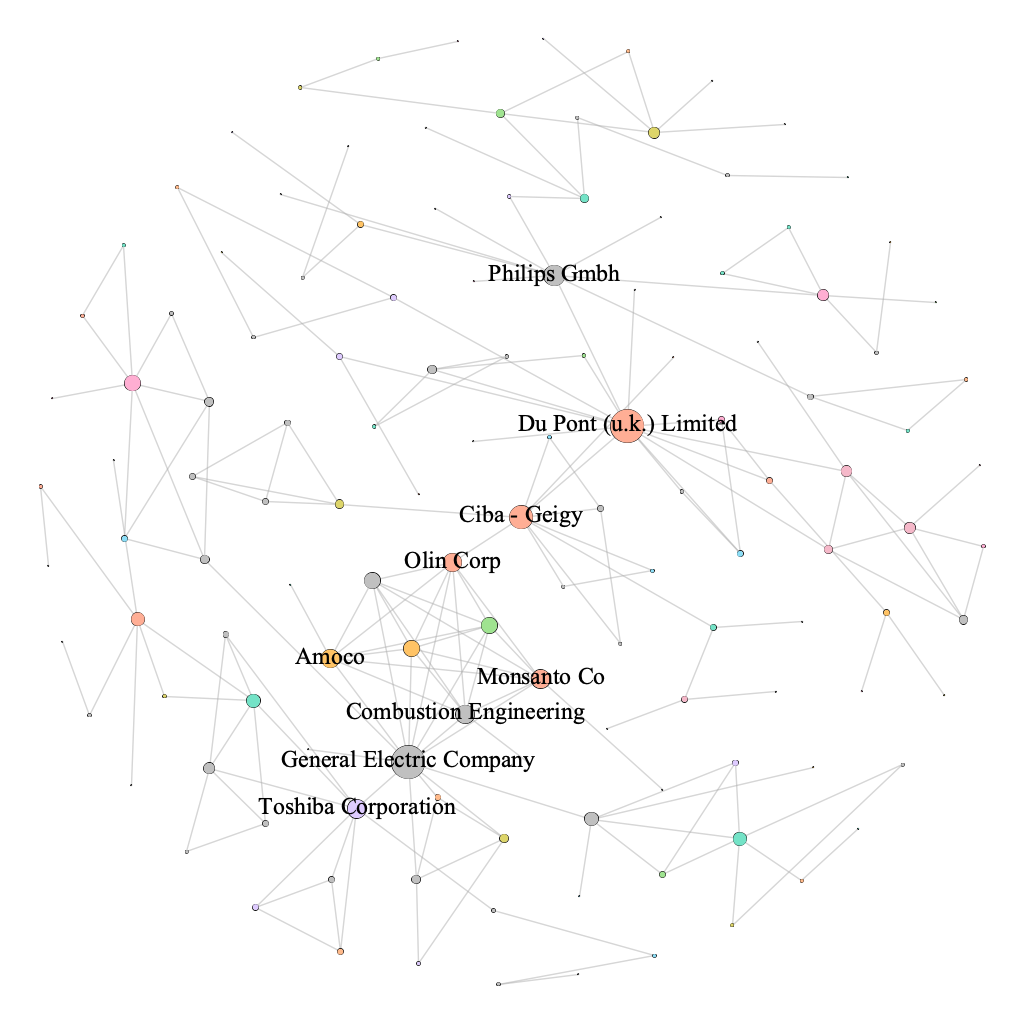
\includegraphics{./Figures/1990_cc_graph_2.png}}}
% \caption{The largest connected component in the observed network of R\&D
% collaborations in the year 1990. The color of a node indicates the sector (at the 2-digit NACE level) and its size scales with the number of R\&D collaborations, with the names of the $9$ largest firms mentioned
% in the graph. The number of firms is $131$ and the number of links in the largest connected component is $193$. }
% \label{fig:1990_cc_graph}
% \end{figure}

% \begin{figure}[tbp]
% \begin{center}
% Year: 2000
% \end{center}
% \vspace{-0.25cm}
% \centering
% \centerline{ \scalebox{0.5}{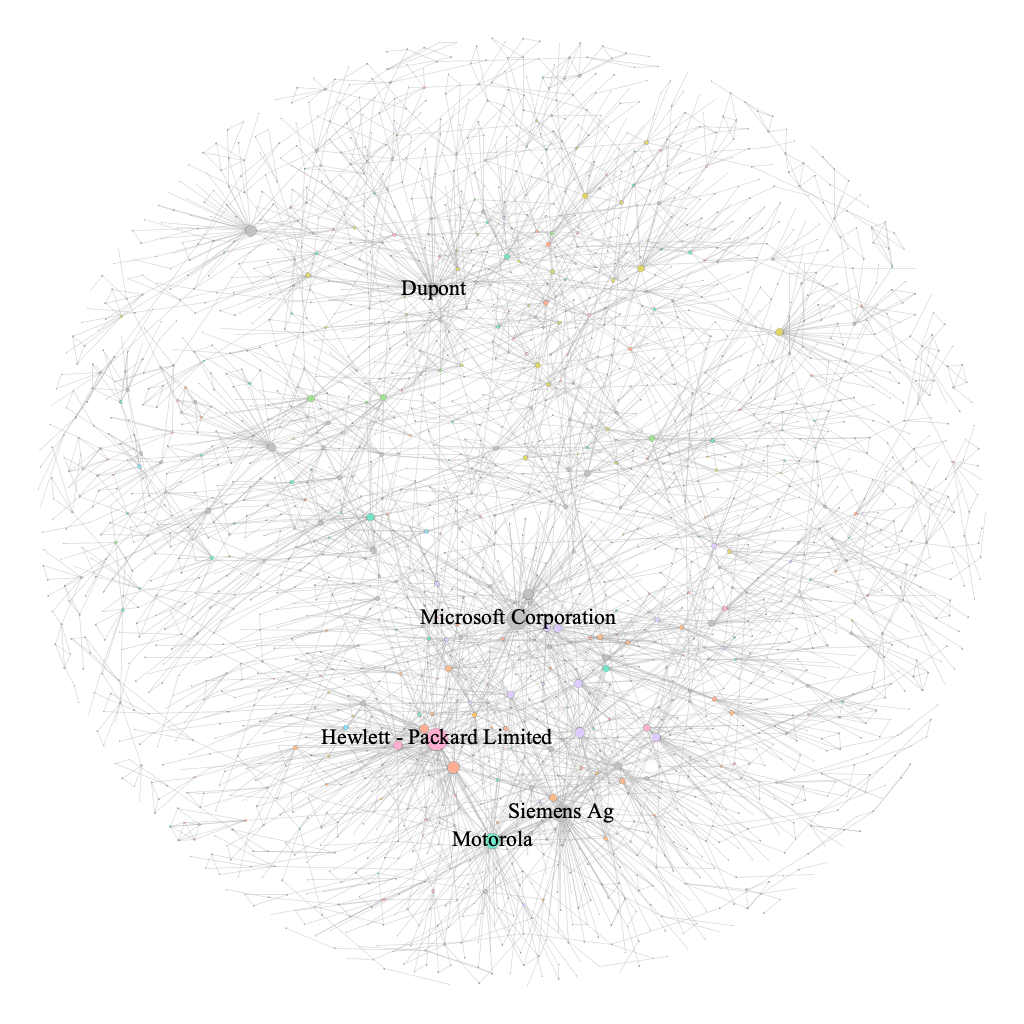
\includegraphics{./Figures/2000_cc_graph_2.png}}}
% \caption{The largest connected component in the observed network of R\&D
% collaborations in the year 2000. The color of a node indicates the sector (at the 2-digit NACE level) and its size scales with the number of R\&D collaborations, with the names of the $5$ largest firms mentioned
% in the graph. The number of links is $4,261$ and the number of firms in the largest connected component is $2,393$. }
% \label{fig:2000_cc_graph}
% \end{figure}

% \begin{figure}[tbp]
% \begin{center}
% Year: 2010
% \end{center}
% \vspace{-0.25cm}
% \centering
% \centerline{ \scalebox{0.5}{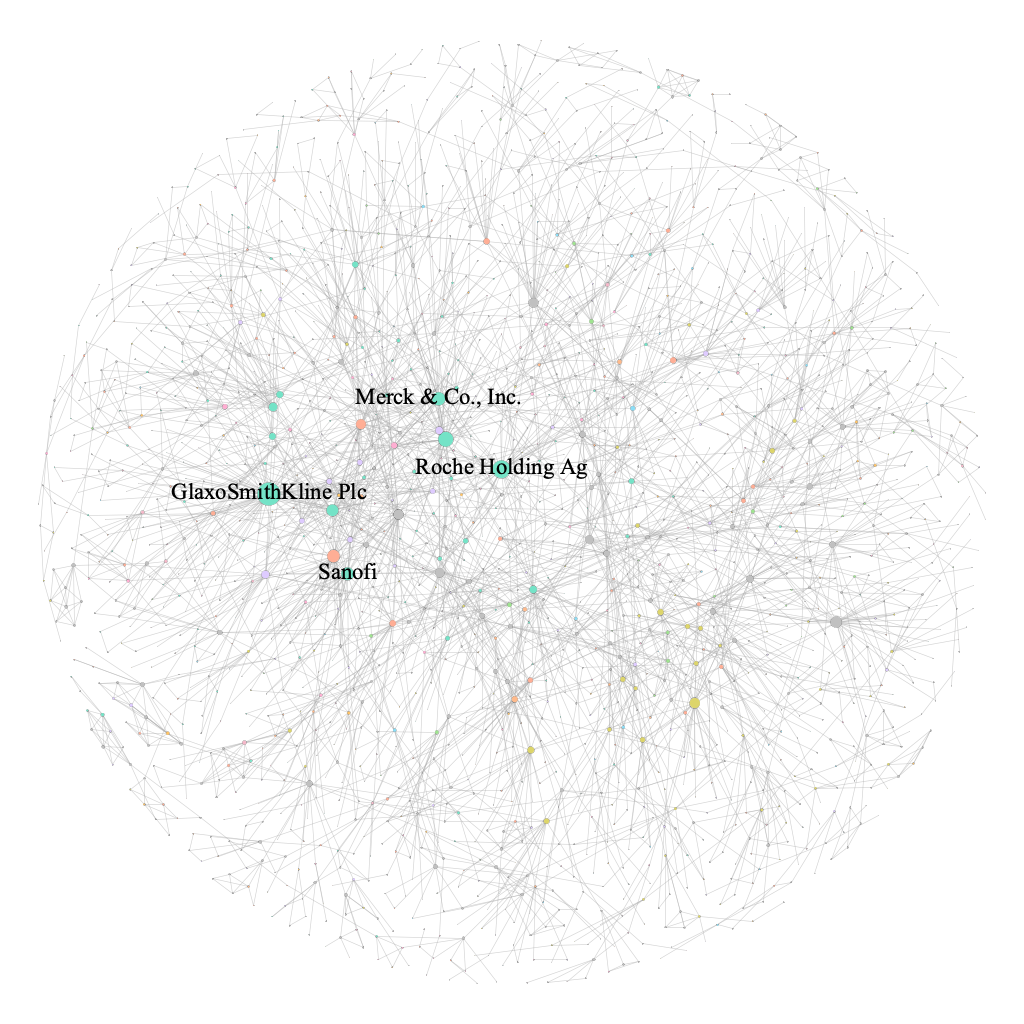
\includegraphics{./Figures/2010_cc_graph_2.png}}}
% \caption{The largest connected component in the observed network of R\&D
% collaborations in the year 2010. The color of a node indicates the sector (at the 2-digit NACE level) and its size scales with the number of R\&D collaborations, with the names of the $4$ largest firms mentioned
% in the graph. The number of links is $3,574$ and the number of firms in the largest connected component is $1,980$. }
% \label{fig:2010_cc_graph}
% \end{figure}

% \begin{figure}[tbp]
% \begin{center}
% Year: 2020
% \end{center}
% \vspace{-0.25cm}
% \centering
% \centerline{ \scalebox{0.5}{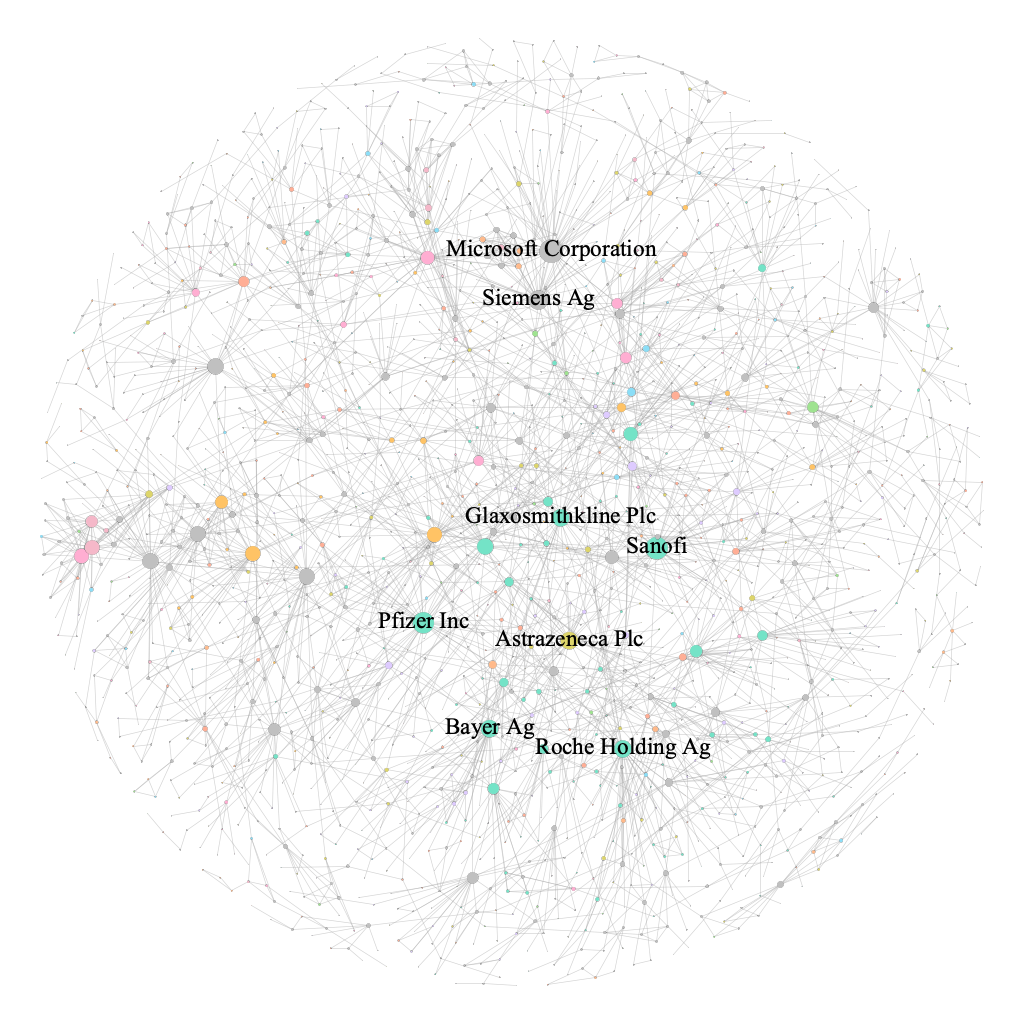
\includegraphics{./Figures/2020_cc_graph_2.png}}}
% \caption{The largest connected component in the observed network of R\&D
% collaborations in the year 2020. The color of a node indicates the sector (at the 2-digit NACE level) and its size scales with the number of R\&D collaborations, with the names of the $8$ largest firms mentioned
% in the graph. The number of links is $3,307$ and the number of firms in the largest connected component is $1,826$. }
% \label{fig:2020_cc_graph}
% \end{figure}

Figure \ref{fig:network-distr} shows the degree distribution, $P(d)$, the average nearest neighbor connectivity (the average degree of the neighbors of a node with degree $d$), $k_{\mathrm{nn}}(d)$, the clustering degree distribution (the average clustering coefficient of a node with degree $d$), $C(d) $,\footnote{\label{foot:clust} The clustering coefficient is the fraction of the number of links between the neighbors of a node divided by the maximum number of links that could possibly exist between the neighbors.} and the component size distribution, $P(s)$. All distributions are highly skewed, indicating a large degree of inequality (indicated with a power-law decay in the upper tails) among firms in the network.
\begin{figure}[tbp]
\begin{minipage}{0.9\linewidth}
\centering
\begin{minipage}{0.49\linewidth}
\centering
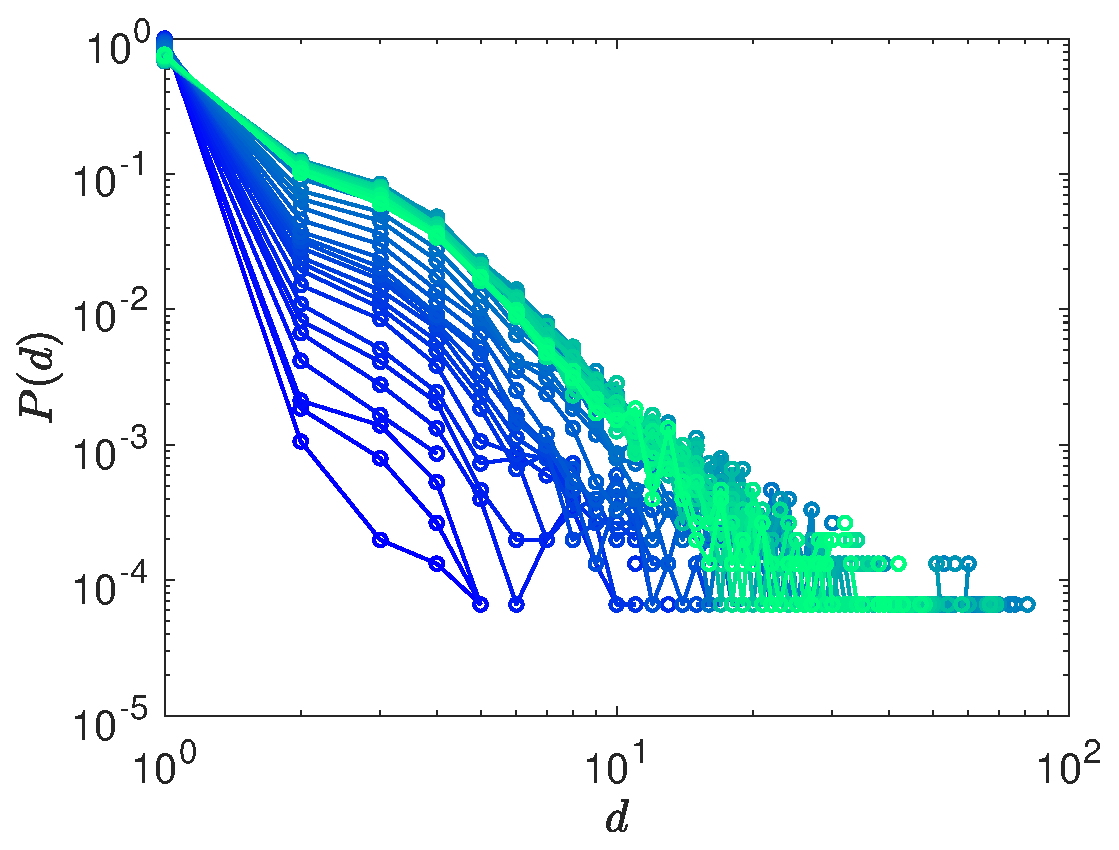
\includegraphics[width=7cm,angle=0]{./Figures/1980_2021_alliance_duration_5_degree_distr.eps}
\end{minipage}
\begin{minipage}{0.49\linewidth}
\centering
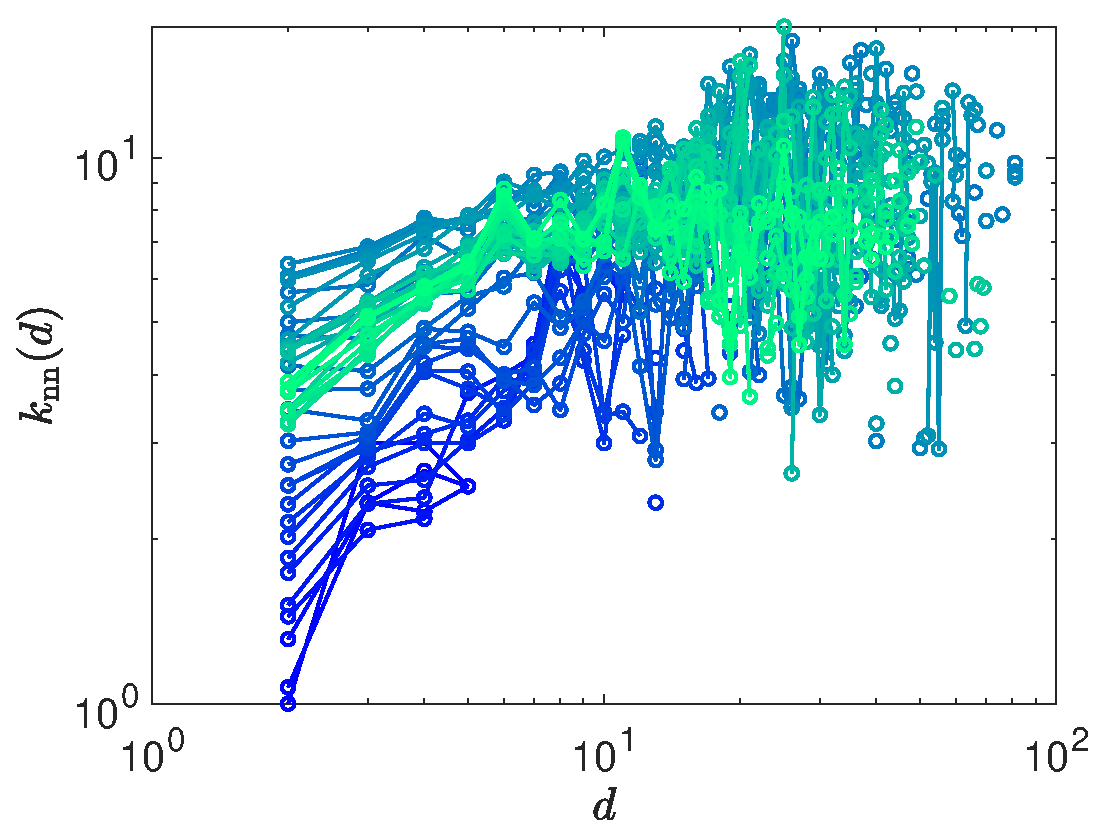
\includegraphics[width=7cm,angle=0]{./Figures/1980_2021_alliance_duration_5_annd_distr.eps}
\end{minipage}
\begin{minipage}{0.49\linewidth}
\centering
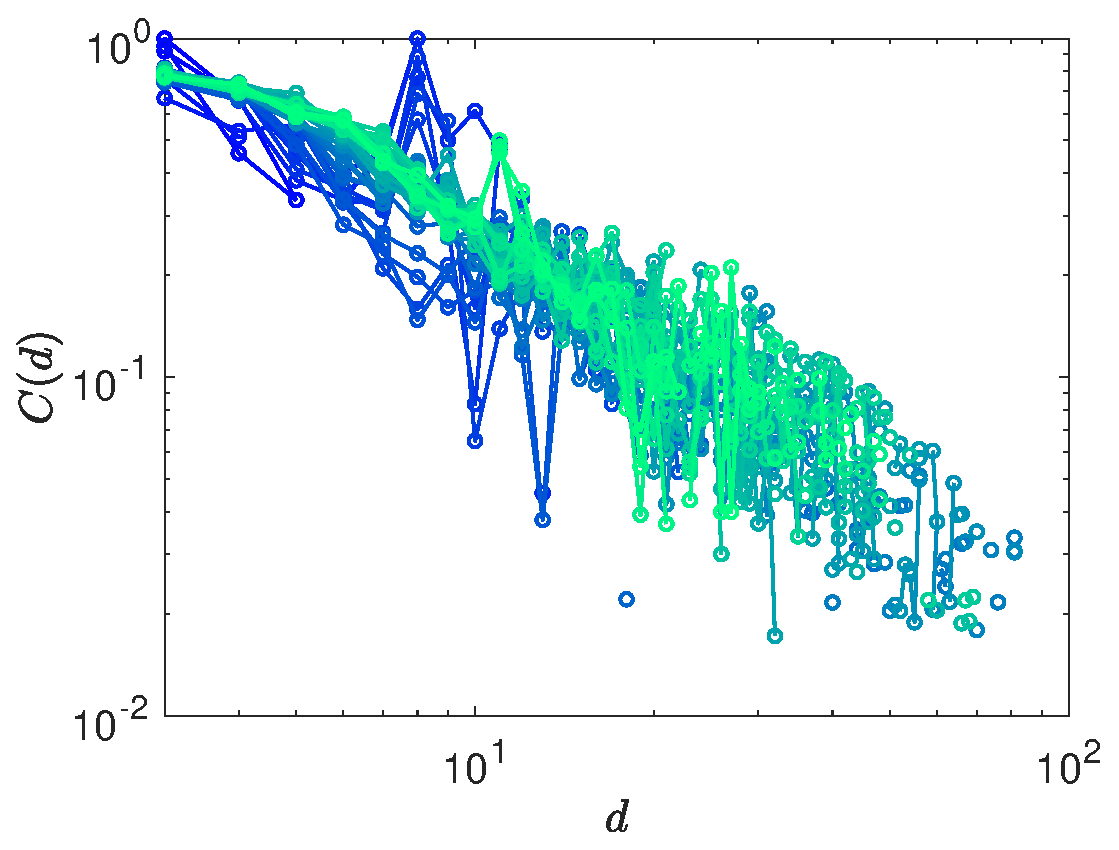
\includegraphics[width=7cm,angle=0]{./Figures/1980_2021_alliance_duration_5_clust_degree_distr.eps}
\end{minipage}
\begin{minipage}{0.49\linewidth}
\centering
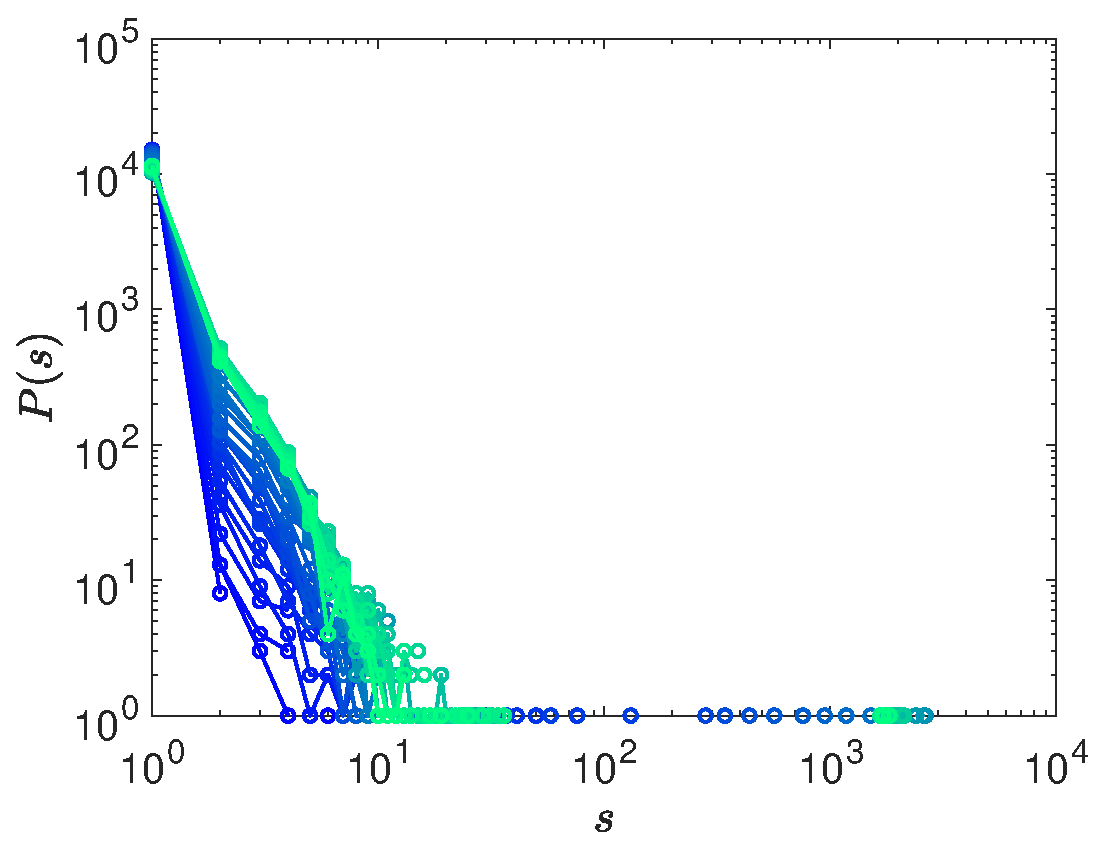
\includegraphics[width=7cm,angle=0]{./Figures/1980_2021_alliance_duration_5_compsizedistr.eps}
\end{minipage}
\end{minipage}
%\hspace{-2.5cm}
\begin{minipage}{0.05\linewidth}
\definecolor{col1}{rgb}{0,0,1}
\definecolor{col2}{rgb}{0,0.032258,0.98387}
\definecolor{col3}{rgb}{0,0.064516,0.96774}
\definecolor{col4}{rgb}{0,0.096774,0.95161}
\definecolor{col5}{rgb}{0,0.12903,0.93548}
\definecolor{col6}{rgb}{0,0.16129,0.91935}
\definecolor{col7}{rgb}{0,0.19355,0.90323}
\definecolor{col8}{rgb}{0,0.22581,0.8871}
\definecolor{col9}{rgb}{0,0.25806,0.87097}
\definecolor{col10}{rgb}{0,0.29032,0.85484}
\definecolor{col11}{rgb}{0,0.32258,0.83871}
\definecolor{col12}{rgb}{0,0.35484,0.82258}
\definecolor{col13}{rgb}{0,0.3871,0.80645}
\definecolor{col14}{rgb}{0,0.41935,0.79032}
\definecolor{col15}{rgb}{0,0.45161,0.77419}
\definecolor{col16}{rgb}{0,0.48387,0.75806}
\definecolor{col17}{rgb}{0,0.51613,0.74194}
\definecolor{col18}{rgb}{0,0.54839,0.72581}
\definecolor{col19}{rgb}{0,0.58065,0.70968}
\definecolor{col20}{rgb}{0,0.6129,0.69355}
\definecolor{col21}{rgb}{0,0.64516,0.67742}
\definecolor{col22}{rgb}{0,0.67742,0.66129}
\definecolor{col23}{rgb}{0,0.70968,0.64516}
\definecolor{col24}{rgb}{0,0.74194,0.62903}
\definecolor{col25}{rgb}{0,0.77419,0.6129}
\definecolor{col26}{rgb}{0,0.80645,0.59677}
\definecolor{col27}{rgb}{0,0.83871,0.58065}
\definecolor{col28}{rgb}{0,0.87097,0.56452}
\definecolor{col29}{rgb}{0,0.90323,0.54839}
\definecolor{col30}{rgb}{0,0.93548,0.53226}
\definecolor{col31}{rgb}{0,0.96774,0.51613}
\definecolor{col32}{rgb}{0,1,0.5}
\colorbox{col1!50}{1990} \\
%\colorbox{col2!50}{1991} \\
\colorbox{col3!50}{1992} \\
%\colorbox{col4!50}{1993} \\
\colorbox{col5!50}{1994} \\
%\colorbox{col6!50}{1995} \\
\colorbox{col7!50}{1996} \\
%\colorbox{col8!50}{1997} \\
\colorbox{col9!50}{1998} \\
%\colorbox{col10!50}{1999} \\
\colorbox{col11!50}{2000} \\
%\colorbox{col12!50}{2001} \\
\colorbox{col13!50}{2002} \\
%\colorbox{col14!50}{2003} \\
\colorbox{col15!50}{2004} \\
%\colorbox{col16!50}{2005} \\
\colorbox{col17!50}{2006} \\
%\colorbox{col18!50}{2007} \\
\colorbox{col19!50}{2008} \\
%\colorbox{col20!50}{2009} \\
\colorbox{col21!50}{2010} \\
%\colorbox{col22!50}{2011} \\
\colorbox{col23!50}{2012} \\
%\colorbox{col24!50}{2013} \\
\colorbox{col25!50}{2014} \\
%\colorbox{col26!50}{2015} \\
\colorbox{col27!50}{2016} \\
%\colorbox{col28!50}{2017} \\
\colorbox{col29!50}{2018} \\
%\colorbox{col30!50}{2019} \\
\colorbox{col31!50}{2020} \\
%\colorbox{col32!50}{2021} \\
\end{minipage}
\caption{The degree distribution, $P(d)$, the average nearest neighbor connectivity, $k_{\mathrm{nn}}(d)$, the clustering degree distribution, $C(d) $, and the component size distribution, $P(s)$.}
\label{fig:network-distr}
\end{figure}

\begin{figure}[tbp]
\begin{minipage}{0.32\linewidth}
\centering
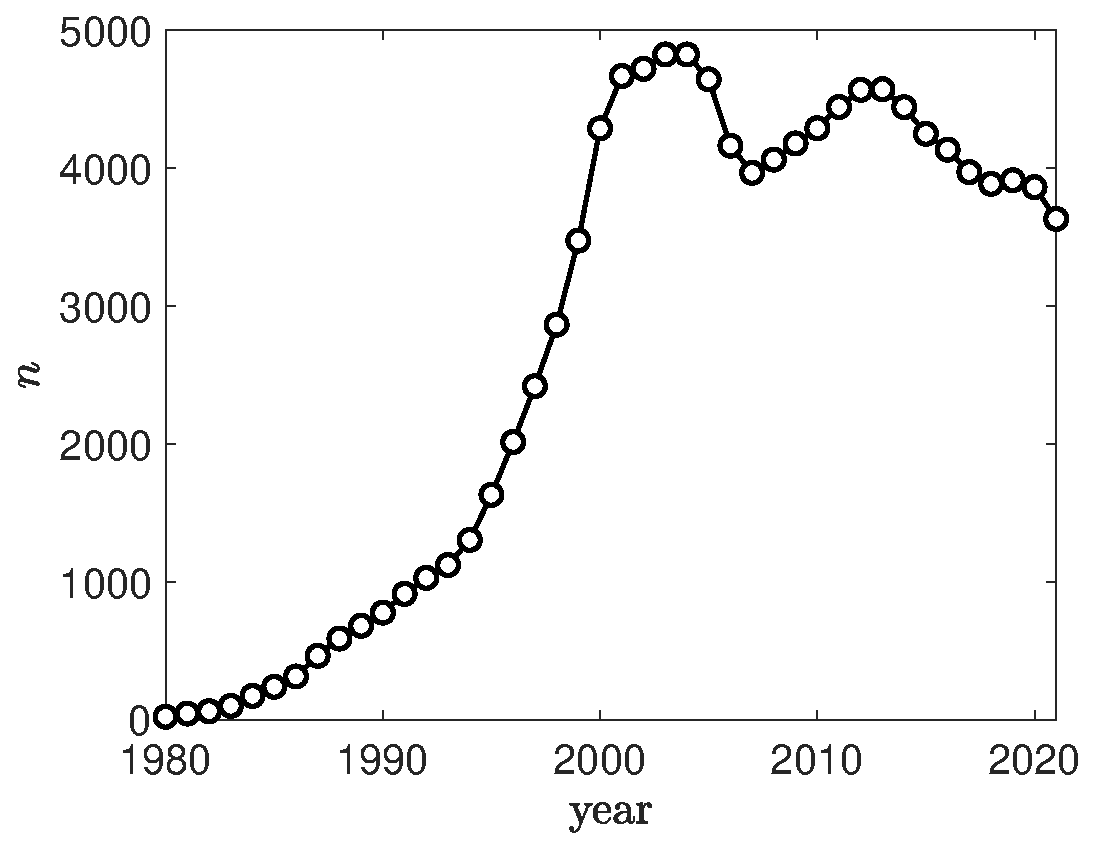
\includegraphics[width=5.4cm,angle=0]{./Figures/1980_2021_alliance_duration_5_num_nodes.eps}
\end{minipage}
\begin{minipage}{0.32\linewidth}
\centering
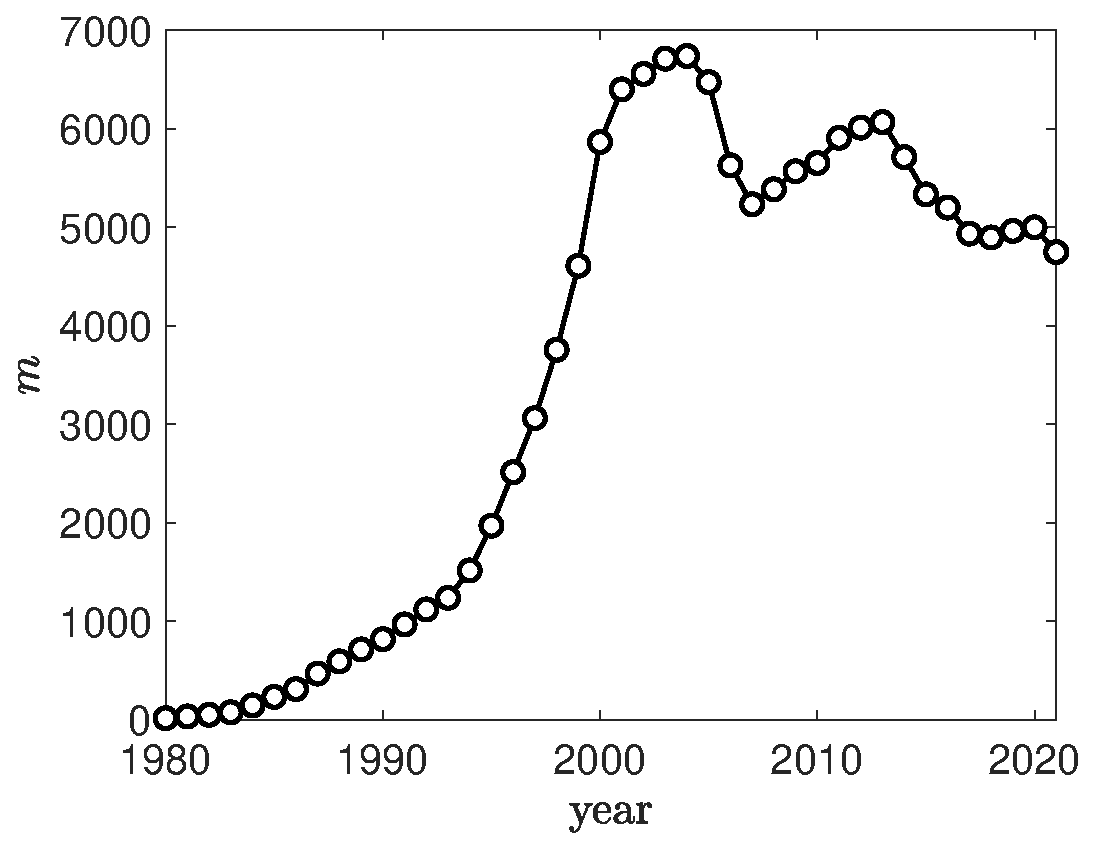
\includegraphics[width=5.4cm,angle=0]{./Figures/1980_2021_alliance_duration_5_num_links.eps}
\end{minipage}
\begin{minipage}{0.32\linewidth}
\centering
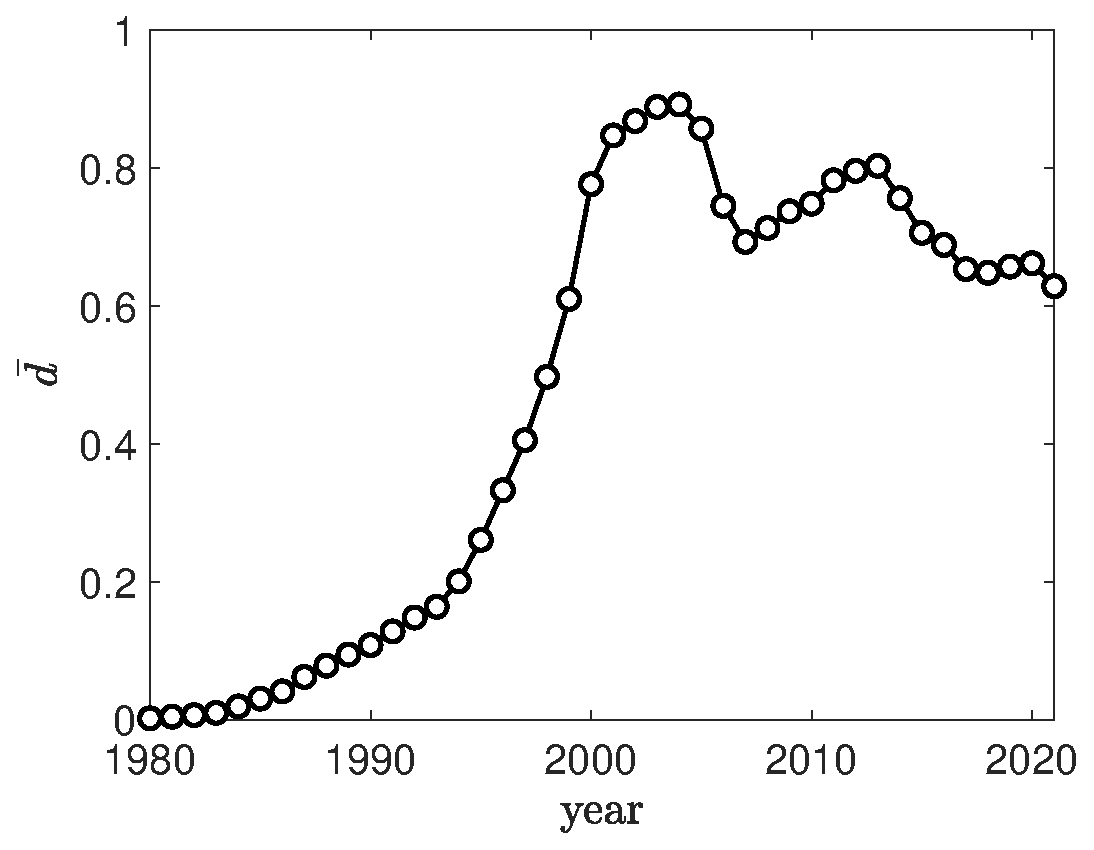
\includegraphics[width=5.4cm,angle=0]{./Figures/1980_2021_alliance_duration_5_av_degree.eps}
\end{minipage}
%
\begin{minipage}{0.32\linewidth}
\centering
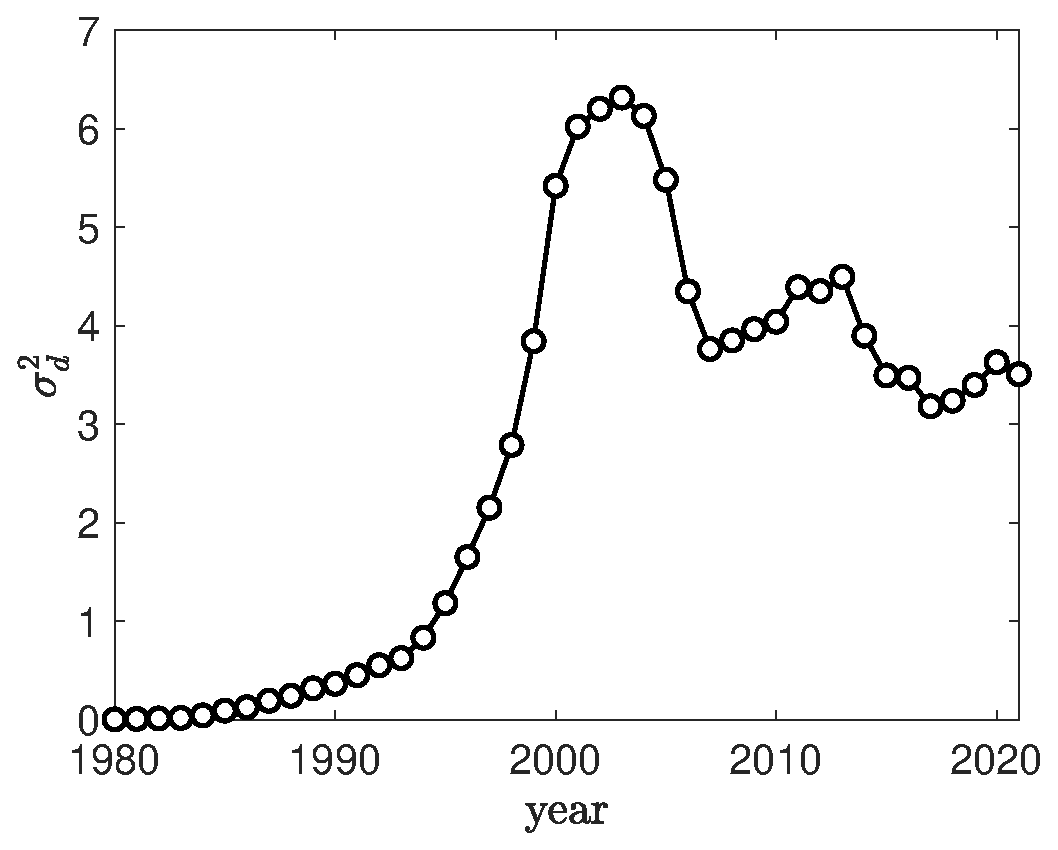
\includegraphics[width=5.4cm,angle=0]{./Figures/1980_2021_alliance_duration_5_degree_var.eps}
\end{minipage}
\begin{minipage}{0.32\linewidth}
\centering
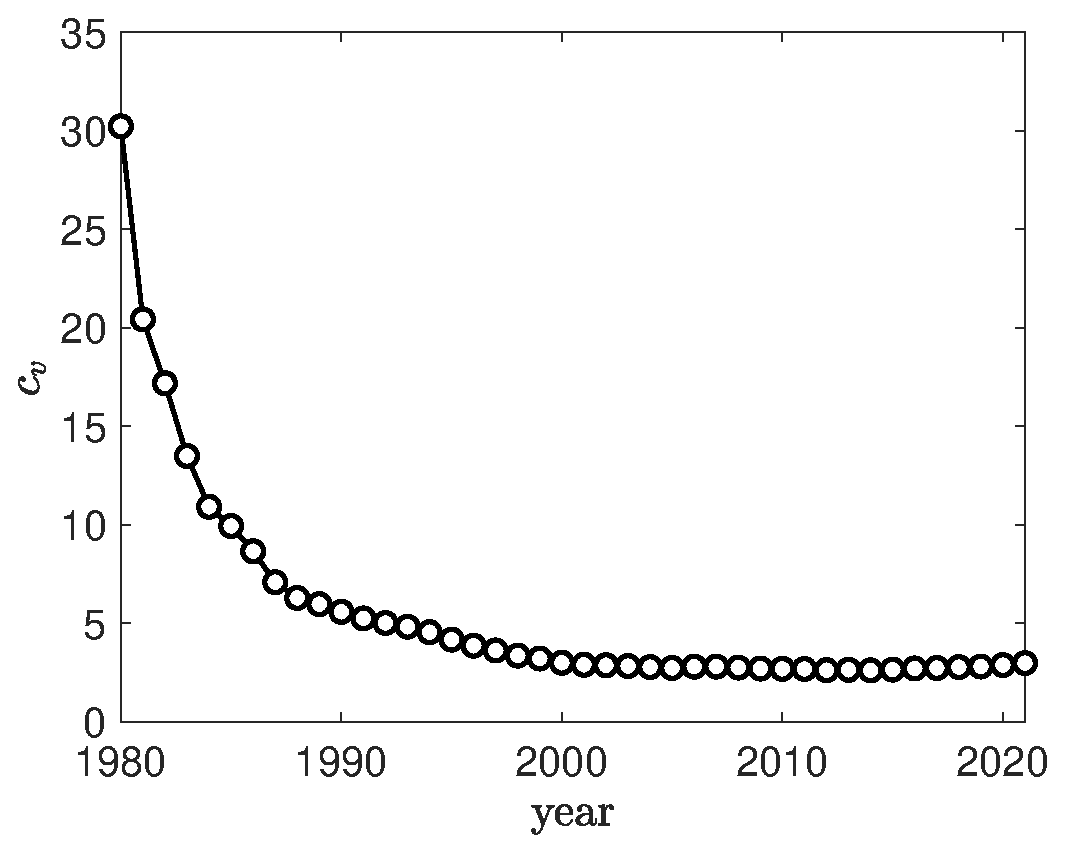
\includegraphics[width=5.4cm,angle=0]{./Figures/1980_2021_alliance_duration_5_coeff_var.eps}
\end{minipage}
\begin{minipage}{0.32\linewidth}
\centering
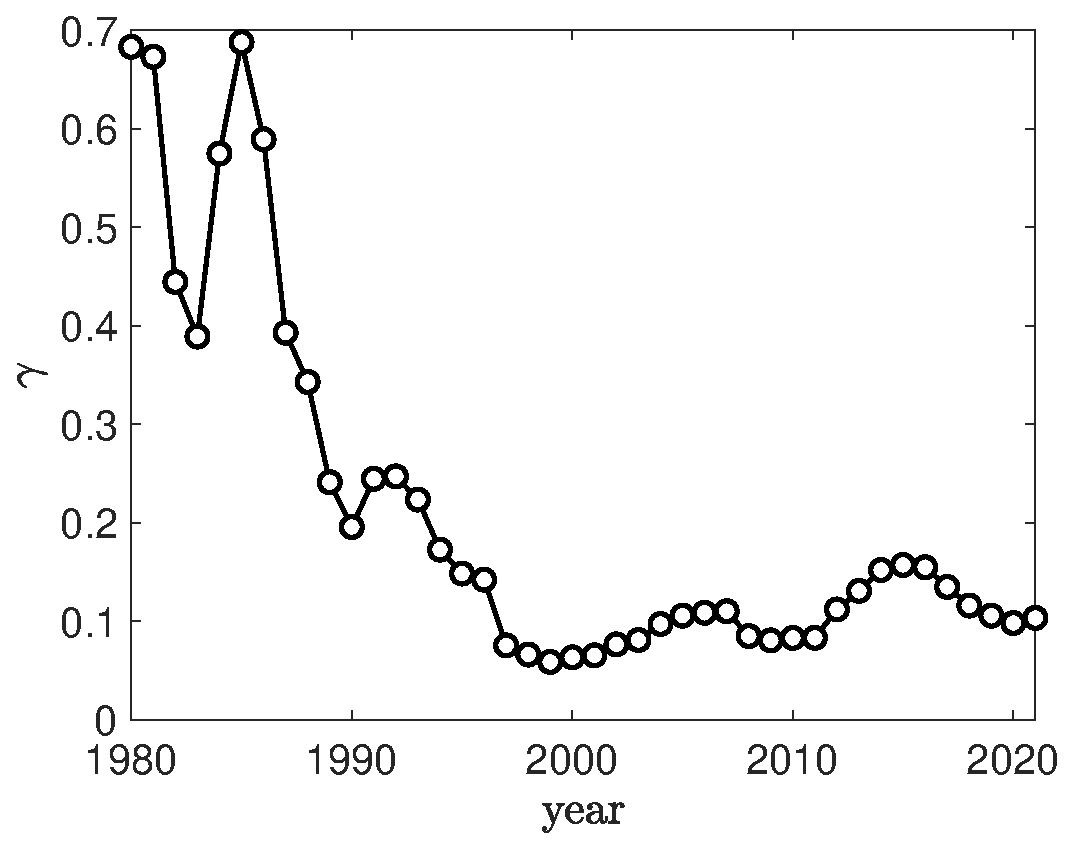
\includegraphics[width=5.4cm,angle=0]{./Figures/1980_2021_alliance_duration_5_assort_coeff.eps}
\end{minipage}
%
\begin{minipage}{0.32\linewidth}
\centering
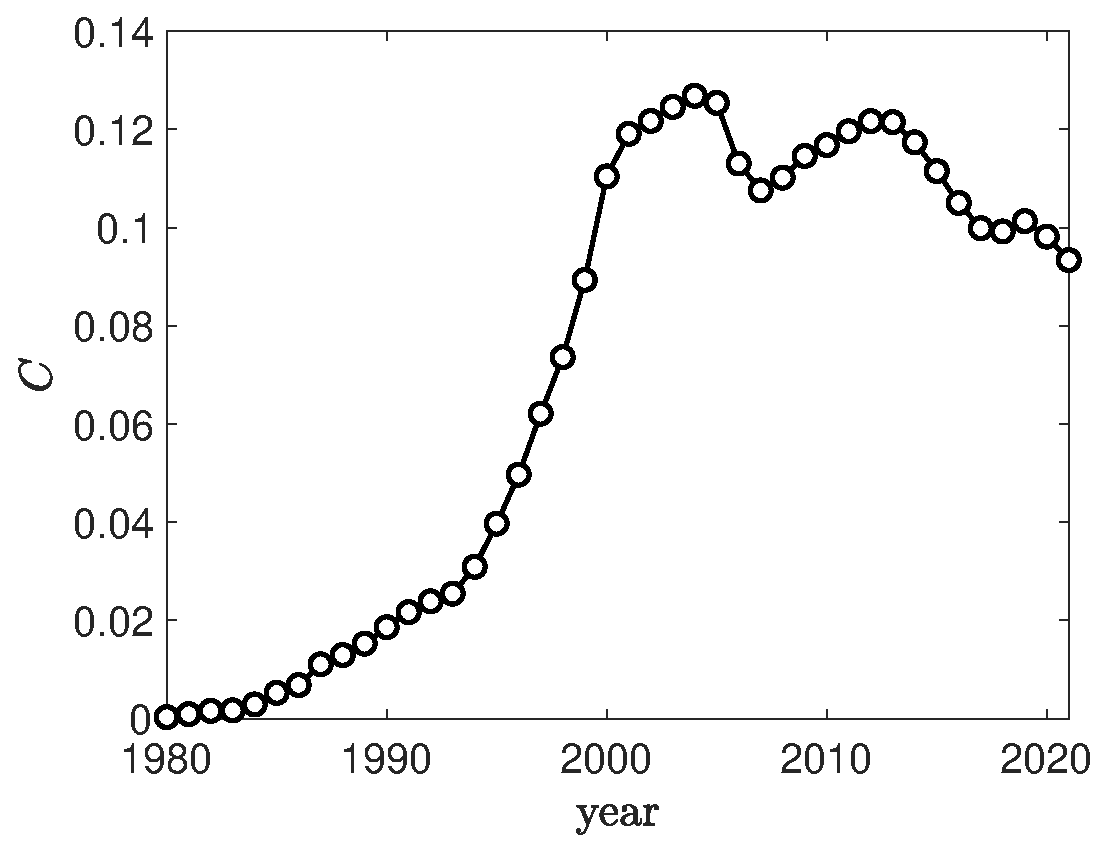
\includegraphics[width=5.4cm,angle=0]{./Figures/1980_2021_alliance_duration_5_clustering.eps}
\end{minipage}
\begin{minipage}{0.32\linewidth}
\centering
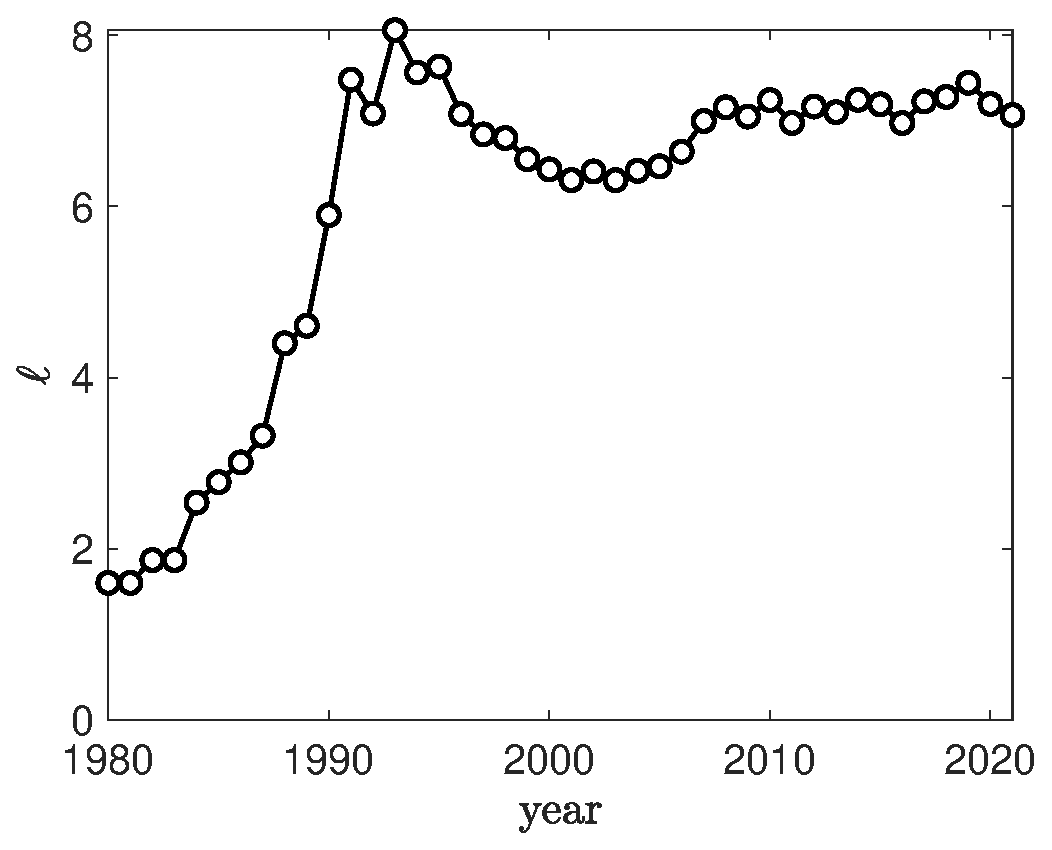
\includegraphics[width=5.4cm,angle=0]{./Figures/1980_2021_alliance_duration_5_averagepathlength.eps}
\end{minipage}
\begin{minipage}{0.32\linewidth}
\centering
\hspace{-0.25cm} 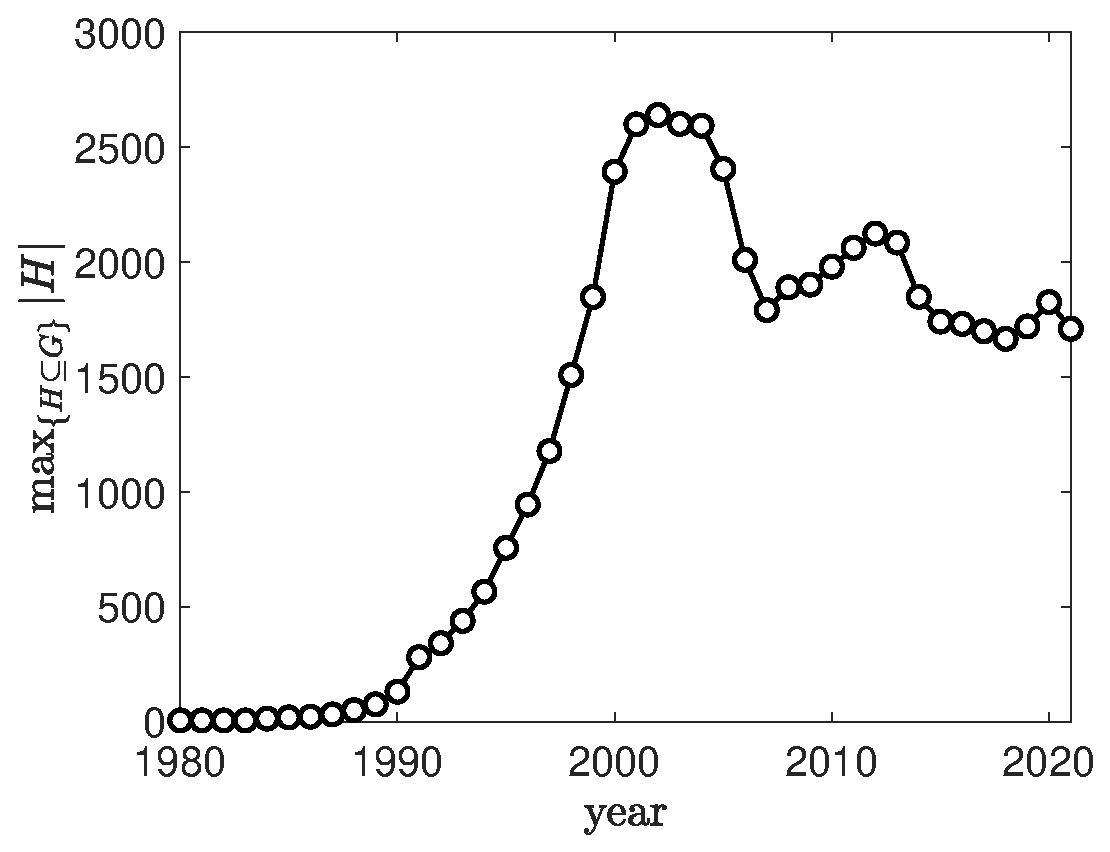
\includegraphics[width=5.4cm,angle=0]{./Figures/1980_2021_alliance_duration_5_compsize.eps}
\end{minipage}
%
\begin{minipage}{0.32\linewidth}
\centering
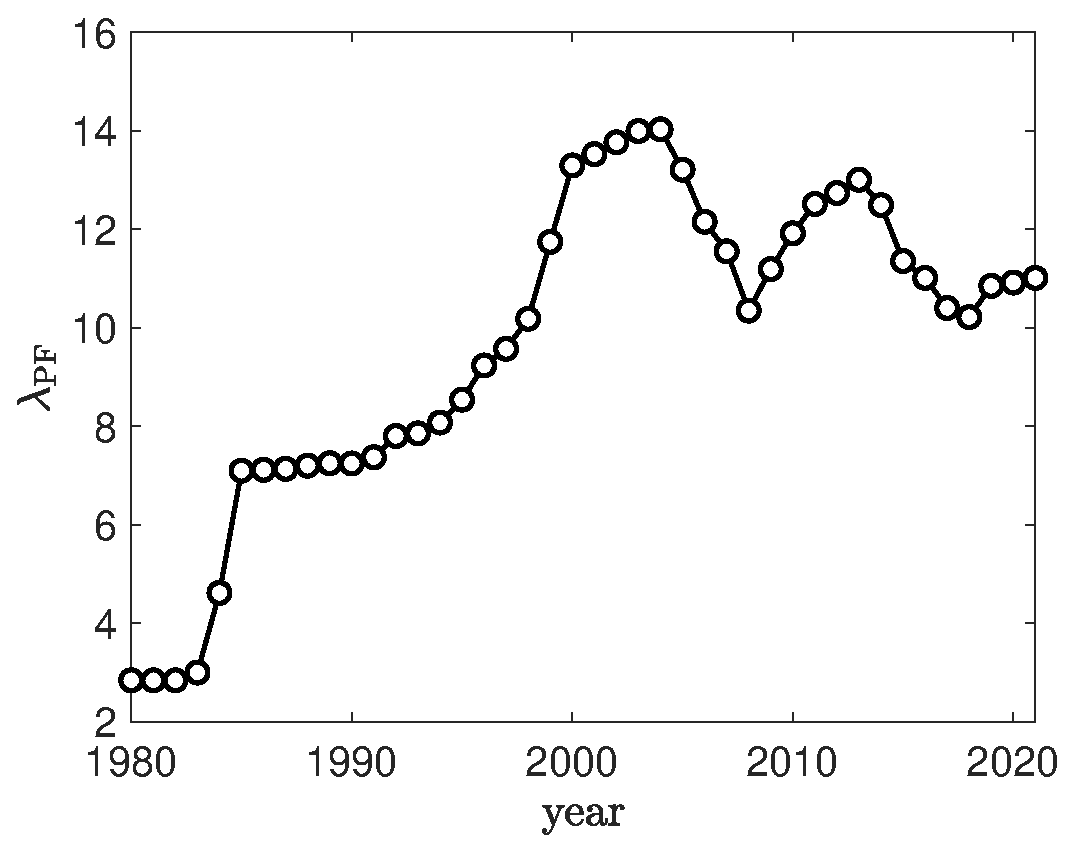
\includegraphics[width=5.4cm,angle=0]{./Figures/1980_2021_alliance_duration_5_eigvalue.eps}
\end{minipage}
\begin{minipage}{0.33\linewidth}
\centering
\hspace{5cm} 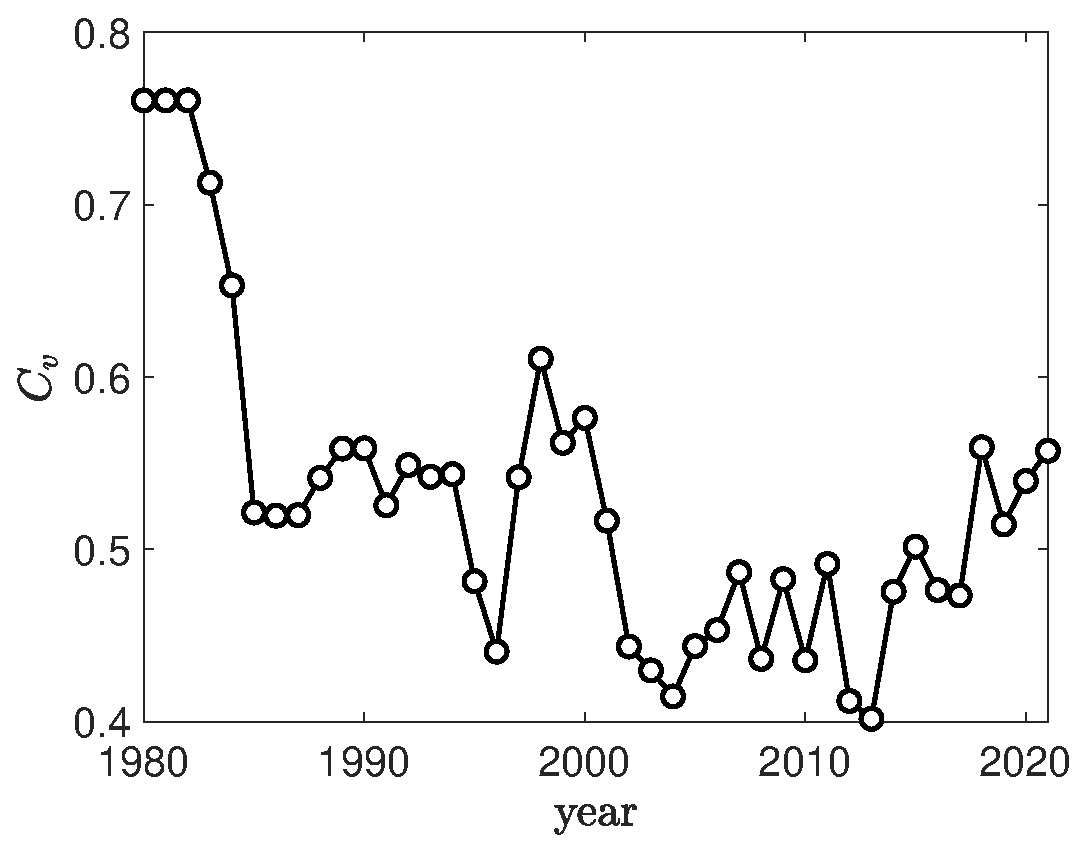
\includegraphics[width=5.4cm,angle=0]{./Figures/1980_2021_alliance_duration_5_eigvcentralization.eps}
\end{minipage}
\begin{minipage}{0.335\linewidth}
\centering
\hspace{5cm}
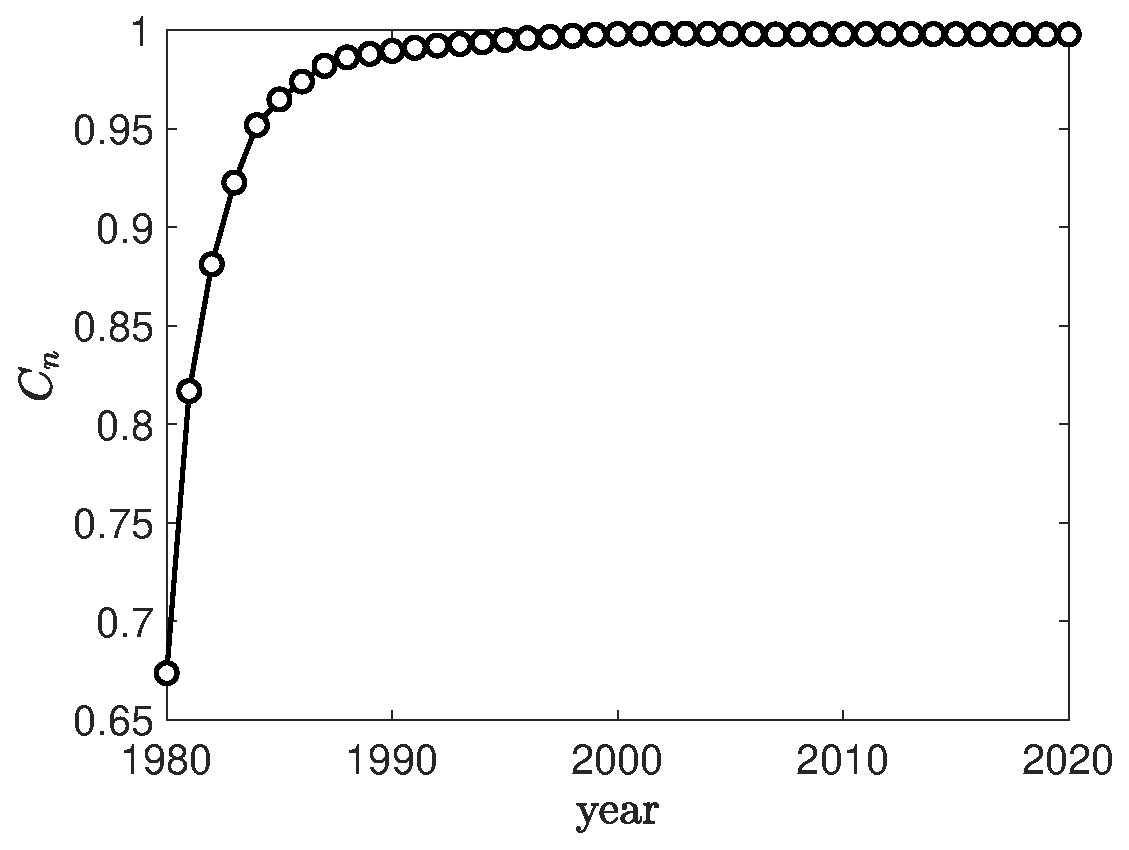
\includegraphics[width=5.4cm,angle=0]{./Figures/1980_2021_nestedness.eps}
\end{minipage}
%\begin{minipage}{0.3\linewidth}
%\centering
%\phantom{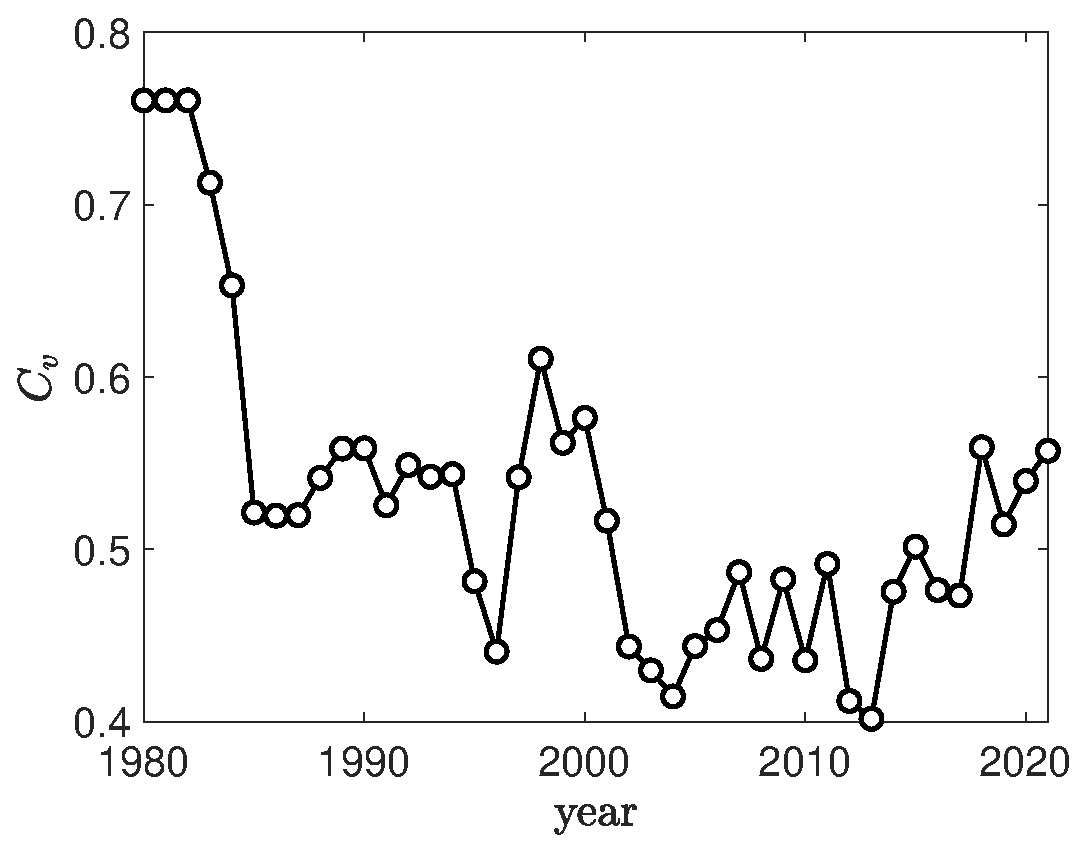
\includegraphics[width=5.5cm,angle=0]{./Figures/1980_2021_alliance_duration_5_eigvcentralization.eps}}
%\end{minipage}
\caption{The number of nodes, $n$, the number of links, $m$, the average degree, $\bar{d}$, the degree variance, $\sigma_d^2$, the degree coefficient of variation (standard deviation divided by the mean), $c_v$, the assortativity coefficient, $\gamma$, the clustering coefficient, $C$, the average path length, $\ell$, the size of the largest connected component, $\max_{H \subseteq G} |H|$, the largest real eigenvalue, $\lambda_{\text{PF}}$, the eigenvector centralization, $C_v$, and the nestedness coefficient, $C_n$.}
\label{fig:network-time-series}
\end{figure}

Figure \ref{fig:network-time-series} shows the evolution of the number of nodes / firms, $n$, the number of links / collaborations, $m$, the average degree, $\bar{d}$, the degree variance, $\sigma_d^2$, the degree coefficient of variation (standard deviation divided by the mean), $c_v$, the assortativity coefficient, $\gamma$, the clustering coefficient, $C$,${}^{\ref{foot:clust}}$ the average path length, $\ell$,\footnote{The average path length is defined as the average number of links along the shortest paths for all possible pairs of nodes in the network.} the size of the largest connected component, $\max_{H \subseteq G} |H|$, the largest real eigenvalue, $\lambda_{\text{PF}}$, and the eigenvector centralization, $C_v$. 

We observe that the number of firms, $n$, the number of links, $m$, the average degree, $\bar{d}$, the degree variance, $\sigma_d^2$, the clustering coefficient, $C$, and the size of the largest connected component, $\max_{H \subseteq G} |H|$, are showing an oscillatory behavior similar to the oscillations documented in \citet{Konig2016a} where an alternative data set on R\&D collaborations has been analyzed. The assortativity coefficient (measuring degree correlations of connected nodes) shows a decreasing trend until the year 2000 indicating that over this time period a transition from an assortative (positive degree correlation) to a dissortative network (negative degree correlation) has taken place. The average path length, $\ell$, is increasing until the year 1995 and stabilizing thereafter. The largest real eigenvalue, $\lambda_{\text{PF}}$, and the eigenvector centralization, $C_v$, of the underlying adjacency matrix of the R\&D network are related to the technology diffusion properties of the R\&D network (as discussed in \citet{koenig09:_effic_and_stabil_of_r_d_networ}). The largest real eigenvalue, $\lambda_{\text{PF}}$ is increasing up to the year 2005 and oscillating thereafter. The eigenvector centralization, $C_v$, is decreasing from an initially high value with a peak in 2000 and shows an increasing trend after 2012.

\citet{Konig2012a} have documented that R\&D networks tend to have a hierarchical structure that can be measured by the ``nestedness'' of the underlying adjacency matrix (see also \citet{Koenig2011}). Nested graphs have a
core-periphery structure
which has also been documented in empirical studies on R\&D networks \citep{Kitsak2010, rosenkopf07:_compar_allian_networ_struc_acros_indus}. We compute the degree of nestedness of a matrix by calculating the \emph{matrix temperature}, $T_n$ \citep{Atmar1993}. Typically, the lower the temperature $T_n$, the higher the degree of nestedness. More precisely, $T_n$ is normalized in such a way that it ranges between $0$ for a perfectly nested matrix and $100$ for a maximally ``unnested'' matrix. From the nestedness temperature we can compute the nestedness coefficient, $C_n$, as $C_n = (100-T_n)/100$, such that $C_n$ ranges from zero for a totally random (non-nested) network to one for a totally nested network \citep{AlmeidaNeto2008}. The bottom right panel in Figure \ref{fig:network-time-series} shows the evolution over time of the nestedness coefficient, $C_n$, with a nestedness coefficient close to one in the years after 2000. 

%\FloatBarrier

%%%%%%%%%%%%%%%%%%%%%%%%%%%%%%%%%%%%%%%%%%%%%%%%%%%%%%%%%
\subsection{Sectoral Composition}
\label{sec:sectors}
%%%%%%%%%%%%%%%%%%%%%%%%%%%%%%%%%%%%%%%%%%%%%%%%%%%%%%%%%
Figures \ref{fig:pie-2-dig-nace} and \ref{fig:pie-3-dig-nace} together with Tables \ref{tab:sic-rank-2-dig} and \ref{tab:sic-rank-3-dig} show the largest sectors in our data at the $2$-digit and $3$-digit NACE Rev. 2 levels, respectively. The dominance of the pharmaceutical sector becomes apparent. However, the sectoral composition is changing over time, as illustrated in Figure \ref{fig:top5-industries}, with pharmaceuticals appearing as the dominant sector only after the year 2005.

\begin{figure}[tbp]
\centering
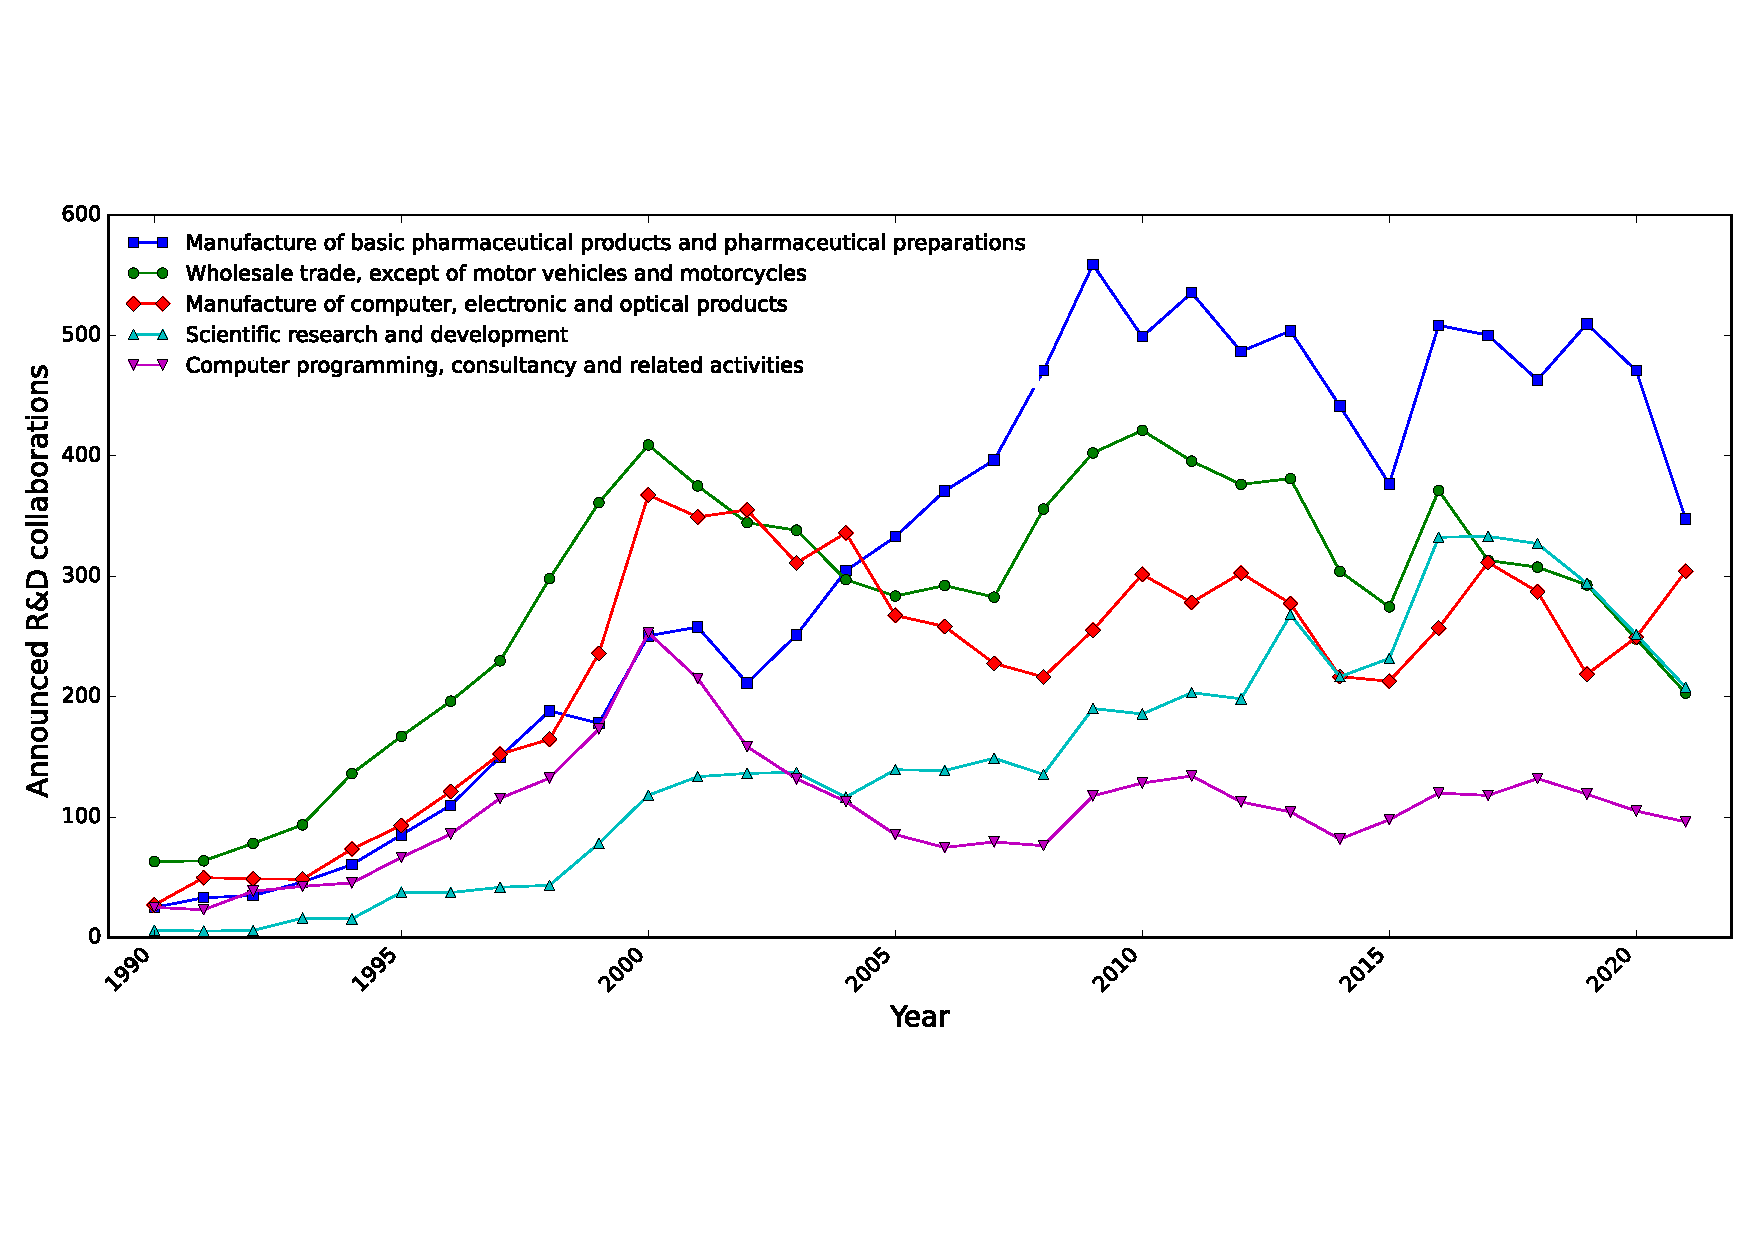
\includegraphics[width=\textwidth,angle=0]{./Figures/rnd_industries_over_time.pdf} 
\caption{R\&D collaborations in the top 5 industries over time. Note that data for 2021 is only partially available (until August 2021).}
\label{fig:top5-industries}
\end{figure}

\begin{figure}[tbp]
\centering
\centerline{ \scalebox{0.75}{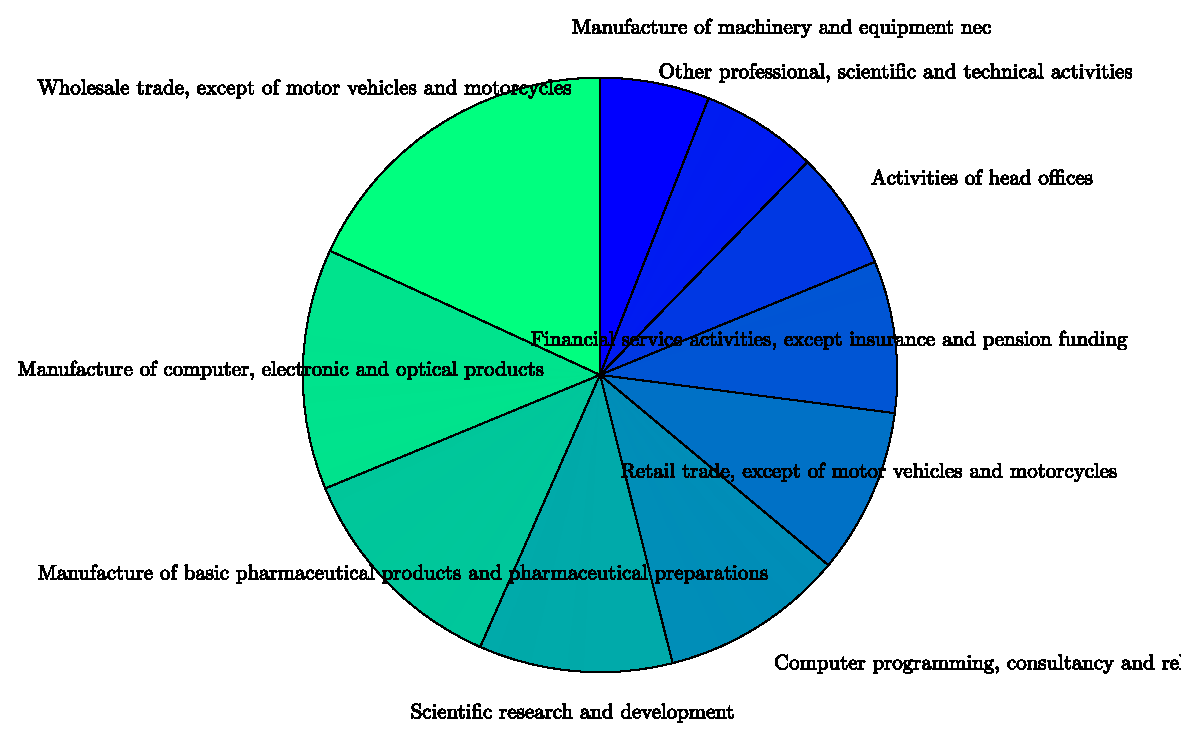
\includegraphics{./Figures/industries_2_dig_nace_distr.eps}}}
\caption{The shares of the ten largest sectors at the $2$-digit NACE Rev. 2 levels. See also Table \ref{tab:sic-rank-2-dig}, respectively. NACE refers to the current Statistical Classification of Economic Activities in the European Community (revision 2).}
\label{fig:pie-2-dig-nace}
\end{figure}

\begin{figure}[tbp]
\centering
\centerline{ \scalebox{0.75}{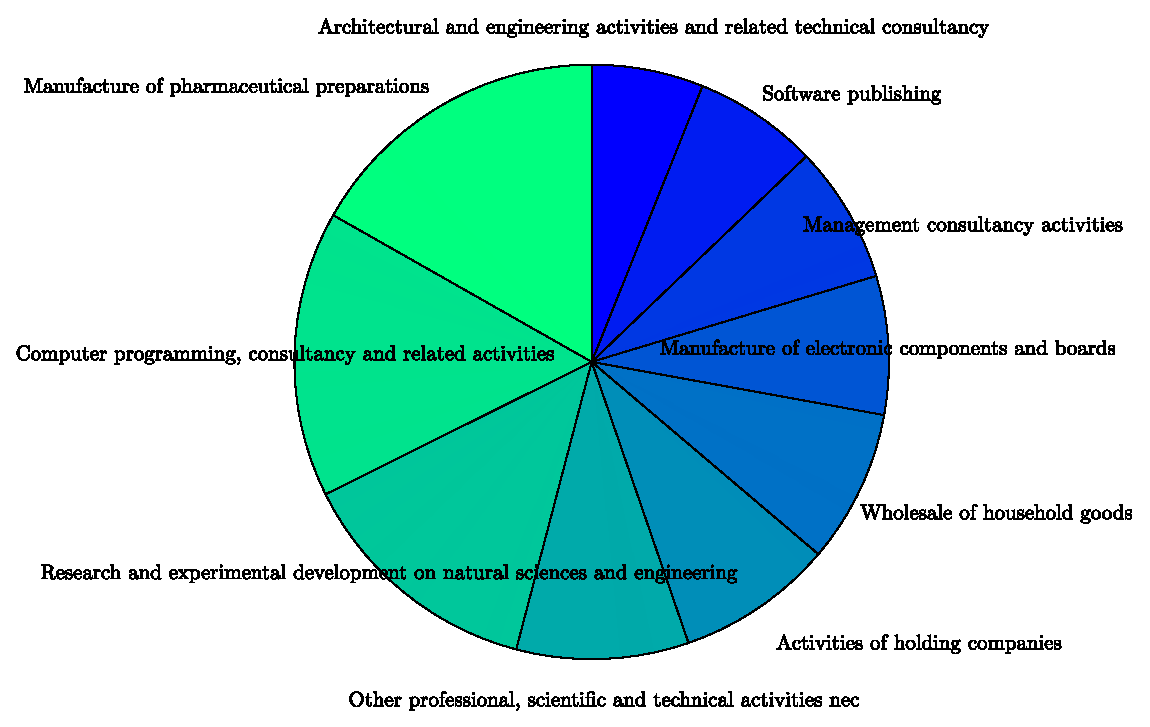
\includegraphics{./Figures/industries_3_dig_nace_distr.eps}}}
\caption{The shares of the ten largest sectors at the $3$-digit NACE Rev. 2 levels. See also Table \ref{tab:sic-rank-3-dig}, respectively. NACE refers to the current Statistical Classification of Economic Activities in the European Community (revision 2).}
\label{fig:pie-3-dig-nace}
\end{figure}

\begin{table}[tpb]
\scalebox{0.9}{
\centering
{\footnotesize
\begin{threeparttable}
\caption{The 20 largest sectors at the $2$-digit NACE Rev. 2 level.}
\label{tab:sic-rank-2-dig}
\begin{tabular}{lcccc}
%ccccccc
\toprule
Sector & 2-dig NACE & $\#$ firms &  $\%$ of tot. & Rank
\\
\midrule
Wholesale trade, except of motor vehicles and motorcycles & 	 46 & 	 1201 & 	 8.43 & 	 1 \\ 
Manufacture of computer, electronic and optical products & 	 26 & 	 867 & 	 6.09 & 	 2 \\ 
Manufacture of basic pharmaceutical products and pharmaceutical preparations & 	 21 & 	 805 & 	 5.65 & 	 3 \\ 
Scientific research and development & 	 72 & 	 697 & 	 4.89 & 	 4 \\ 
Computer programming, consultancy and related activities & 	 62 & 	 663 & 	 4.66 & 	 5 \\ 
Retail trade, except of motor vehicles and motorcycles & 	 47 & 	 596 & 	 4.19 & 	 6 \\ 
Financial service activities, except insurance and pension funding & 	 64 & 	 547 & 	 3.84 & 	 7 \\ 
Activities of head offices & 	 70 & 	 430 & 	 3.02 & 	 8 \\ 
Other professional, scientific and technical activities & 	 74 & 	 420 & 	 2.95 & 	 9 \\ 
Manufacture of machinery and equipment nec & 	 28 & 	 394 & 	 2.77 & 	 10 \\ 
Human health activities & 	 86 & 	 394 & 	 2.77 & 	 11 \\ 
Publishing activities & 	 58 & 	 361 & 	 2.54 & 	 12 \\ 
Manufacture of chemicals and chemical products & 	 20 & 	 360 & 	 2.53 & 	 13 \\ 
Specialised construction activities & 	 43 & 	 315 & 	 2.21 & 	 14 \\ 
Telecommunications & 	 61 & 	 310 & 	 2.18 & 	 15 \\ 
Architectural and engineering activities & 	 71 & 	 305 & 	 2.14 & 	 16 \\ 
Other manufacturing & 	 32 & 	 299 & 	 2.10 & 	 17 \\ 
Activities auxiliary to financial services and insurance activities & 	 66 & 	 265 & 	 1.86 & 	 18 \\ 
Manufacture of fabricated metal products, except machinery and equipment & 	 25 & 	 251 & 	 1.76 & 	 19 \\ 
Office administrative, office support and other business support activities & 	 82 & 	 247 & 	 1.73 & 	 20 \\ 
\midrule
\bottomrule
\end{tabular}
        \begin{tablenotes}[flushleft]%
	\item \emph{Note:} NACE refers to the current Statistical Classification of Economic Activities in the European Community (revision 2).
	\end{tablenotes}
\end{threeparttable}
}
}
\end{table}

\begin{table}[tpb]
\scalebox{0.9}{
\centering
{\footnotesize
\begin{threeparttable}
\caption{The 20 largest sectors at the $3$-digit NACE Rev. 2 level.}
\label{tab:sic-rank-3-dig}
\begin{tabular}{lcccc}
%ccccccc
\toprule
Sector & 3-dig NACE & $\#$ firms &  $\%$ of tot. & Rank
\\
\midrule
Manufacture of pharmaceutical preparations & 	 212 & 	 715 & 	 5.02 & 	 1 \\ 
Computer programming, consultancy and related activities & 	 620 & 	 663 & 	 4.66 & 	 2 \\ 
Research and experimental development on natural sciences and engineering & 	 721 & 	 578 & 	 4.06 & 	 3 \\ 
Other professional, scientific and technical activities & 	 749 & 	 399 & 	 2.80 & 	 4 \\ 
Activities of holding companies & 	 642 & 	 363 & 	 2.55 & 	 5 \\ 
Wholesale of household goods & 	 464 & 	 355 & 	 2.49 & 	 6 \\ 
Manufacture of electronic components and boards & 	 261 & 	 321 & 	 2.25 & 	 7 \\ 
Management consultancy activities & 	 702 & 	 319 & 	 2.24 & 	 8 \\ 
Software publishing & 	 582 & 	 288 & 	 2.02 & 	 9 \\ 
Architectural and engineering activities and related technical consultancy & 	 711 & 	 259 & 	 1.82 & 	 10 \\ 
Other telecommunications activities & 	 619 & 	 240 & 	 1.69 & 	 11 \\ 
Retail sale of other goods in specialised stores & 	 477 & 	 219 & 	 1.54 & 	 12 \\ 
Other human health activities & 	 869 & 	 212 & 	 1.49 & 	 13 \\ 
Activities auxiliary to financial services, except insurance and pension funding & 	 661 & 	 202 & 	 1.42 & 	 14 \\ 
Other specialised wholesale & 	 467 & 	 196 & 	 1.38 & 	 15 \\ 
Manufacture of medical and dental instruments and supplies & 	 325 & 	 191 & 	 1.34 & 	 16 \\ 
Business support service activities nec & 	 829 & 	 188 & 	 1.32 & 	 17 \\ 
Construction of residential and non-residential buildings & 	 412 & 	 181 & 	 1.27 & 	 18 \\ 
Non-specialised wholesale trade & 	 469 & 	 181 & 	 1.27 & 	 19 \\ 
Manufacture of instruments and appliances for measuring, testing and navigation & 	 265 & 	 173 & 	 1.21 & 	 20 \\ 
\midrule
\bottomrule
\end{tabular}
        \begin{tablenotes}[flushleft]%
	\item \emph{Note:} NACE refers to the current Statistical Classification of Economic Activities in the European Community (revision 2).
	\end{tablenotes}
\end{threeparttable}}
}
\end{table}

%\begin{figure}[tbp]
%\begin{minipage}{0.9\linewidth}
%\begin{minipage}{0.49\linewidth}
%\centering
%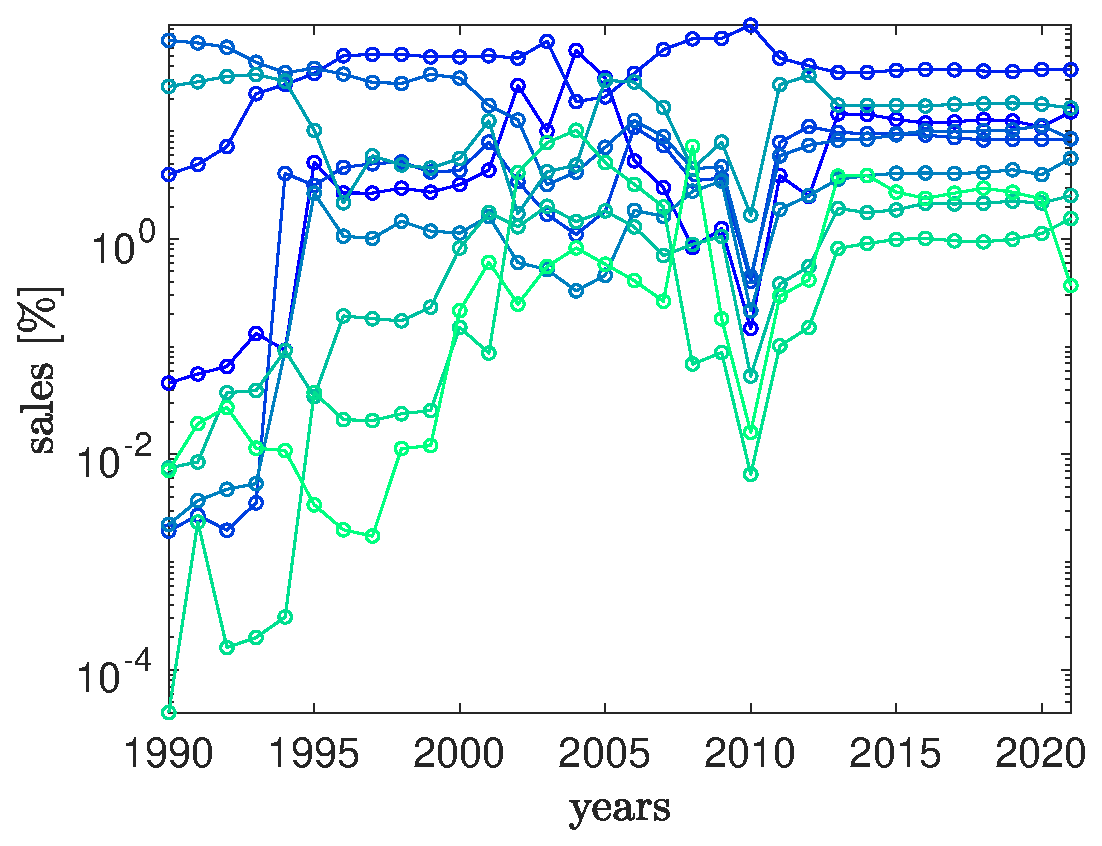
\includegraphics[width=7cm,angle=0]{./Figures/1990_2021_nace_1_dig_frac_sales.eps}
%\end{minipage}
%\begin{minipage}{0.49\linewidth}
%\centering
%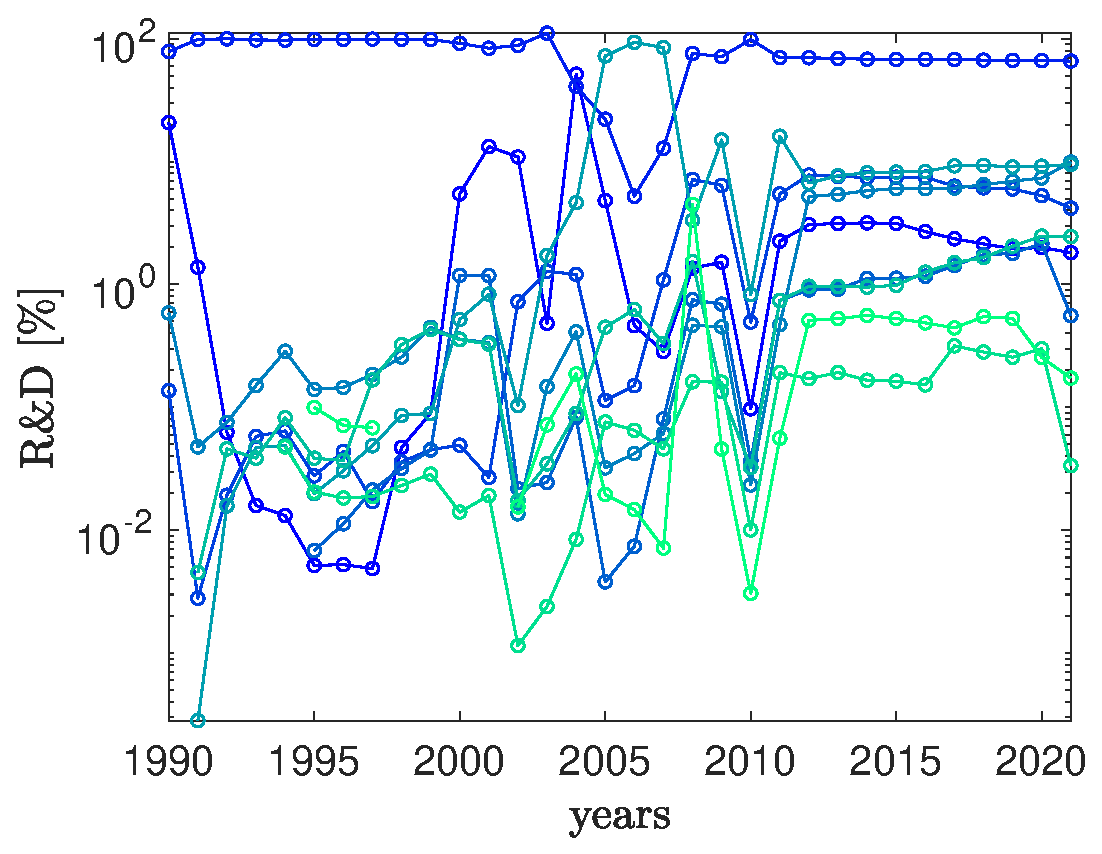
\includegraphics[width=7cm,angle=0]{./Figures/1990_2021_nace_1_dig_frac_rnd.eps}
%\end{minipage}
%\end{minipage}
%\begin{minipage}{0.05\linewidth}
%\vspace{-0.5cm}
%\tiny{
%\definecolor{col1}{rgb}{0,0,1}
%\definecolor{col2}{rgb}{0,0.125,0.9375}
%\definecolor{col3}{rgb}{0,0.25,0.875}
%\definecolor{col4}{rgb}{0,0.375,0.8125}
%\definecolor{col5}{rgb}{0,0.5,0.75}
%\definecolor{col6}{rgb}{0,0.625,0.6875}
%\definecolor{col7}{rgb}{0,0.75,0.625}
%\definecolor{col8}{rgb}{0,0.875,0.5625}
%\definecolor{col9}{rgb}{0,1,0.5}
%\colorbox{col1!50}{NACE: 1} \\
%\colorbox{col2!50}{NACE: 2} \\
%\colorbox{col3!50}{NACE: 3} \\
%\colorbox{col4!50}{NACE: 4} \\
%\colorbox{col5!50}{NACE: 5} \\
%\colorbox{col6!50}{NACE: 6} \\
%\colorbox{col7!50}{NACE: 7} \\
%\colorbox{col8!50}{NACE: 8} \\
%\colorbox{col9!50}{NACE: 9} 
%}
%\end{minipage}
%\caption{Evolution of the shares of total sales (left panel) and total R\&D expenditures (right panel) for different 1-digit NACE codes across time.}
%\label{fig:herfindahl}
%\end{figure}

%%%%%%%%%%%%%%%%%%%%%%%%%%%%%%%%%%%%%%%%%%%%%%%%%%%%%%%%%%
%\subsection{\protect Mergers and Acquisitions}
%\label{sec:mergers}
%%%%%%%%%%%%%%%%%%%%%%%%%%%%%%%%%%%%%%%%%%%%%%%%%%%%%%%%%%
%TODO

%\FloatBarrier

%%%%%%%%%%%%%%%%%%%%%%%%%%%%%%%%%%%%%%%%%%%%%%%%%%%%%%%%%%
\subsection{\protect Balance Sheet Statements, R\&D and
Productivity}
\label{sec:data-balance-sheets}
%%%%%%%%%%%%%%%%%%%%%%%%%%%%%%%%%%%%%%%%%%%%%%%%%%%%%%%%%%
We matched the firms in our R\&D collaboration database with Bureau van Dijk
(BvD)'s Orbis database to obtain information about their balance sheets and income statements. The Orbis database is a
commercial dataset, which contains administrative data on 130 million firms
worldwide. Orbis is an umbrella product that provides firm-level data
covering over 120 countries, both developed and emerging, since 2005. The
financial and balance-sheet information in Orbis comes from business
registers collected by the local Chambers of Commerce to fullfill legal and
administrative requirements and are relayed to BvD via over 40 different
information providers. Orbis contains not only information about publicly listed firms, but provides also information about private firms.\footnote{For further discussion of the
 Orbis databases see \citet[][]{Dai2012}, \citet{Bloom2013} and \citet[][]{Papadopoulos2012}.}

For the matching of firms across datasets we adopted the name matching algorithm developed as part of the NBER patent data project \citep[][]{Trajtenberg2009}. We could match $92.5\%$ of the firms with the Orbis database.

Figure \ref{fig:balance-sheet-distributions} shows the sales, output (deflated sales), R\&D expenditures, and the productivity (value added per worker) distribution for different years ranging from 1990 to 2020. All distributions are highly skewed, indicating a large degree of inequality (indicated with a power-law decay in the upper tails) in firms' sizes,
R\&D expenditures and productivity.
\begin{figure}[tbp]
\begin{minipage}{0.9\linewidth}
\centering
\begin{minipage}{0.49\linewidth}
\centering
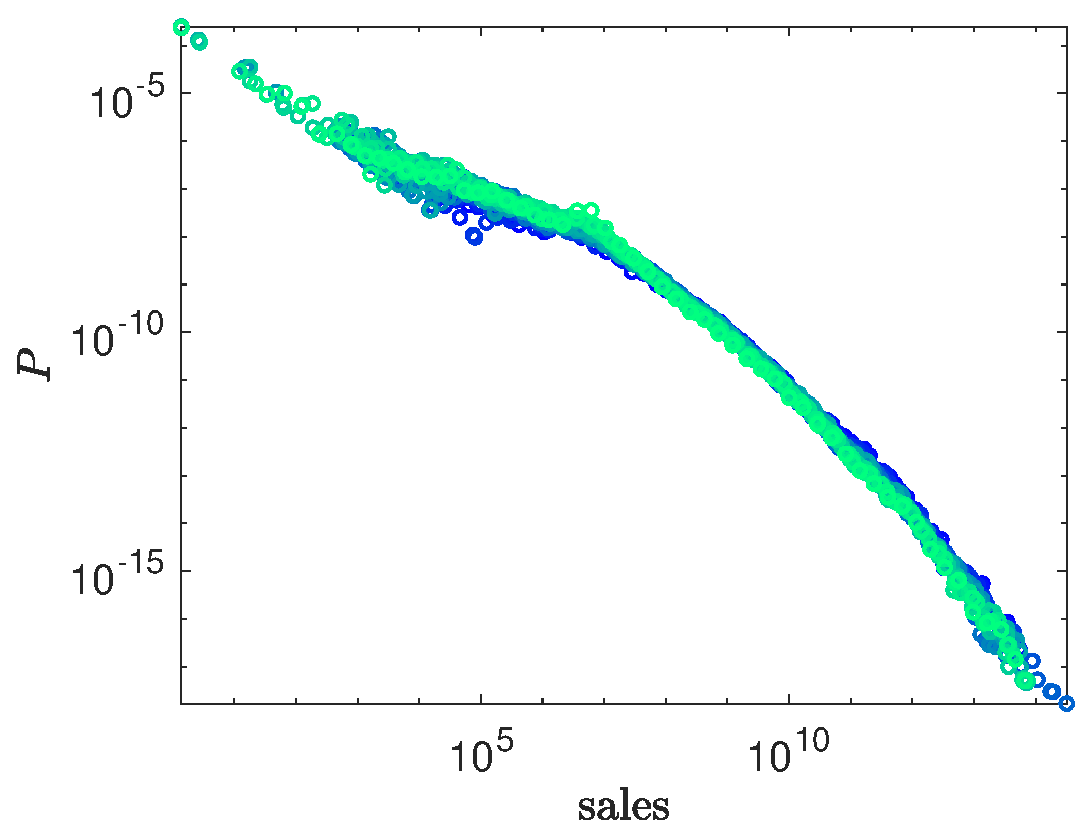
\includegraphics[width=7cm,angle=0]{./Figures/1990_2021_sales_distr.eps}
\vspace{0.5cm}
\end{minipage}
\begin{minipage}{0.49\linewidth}
\centering
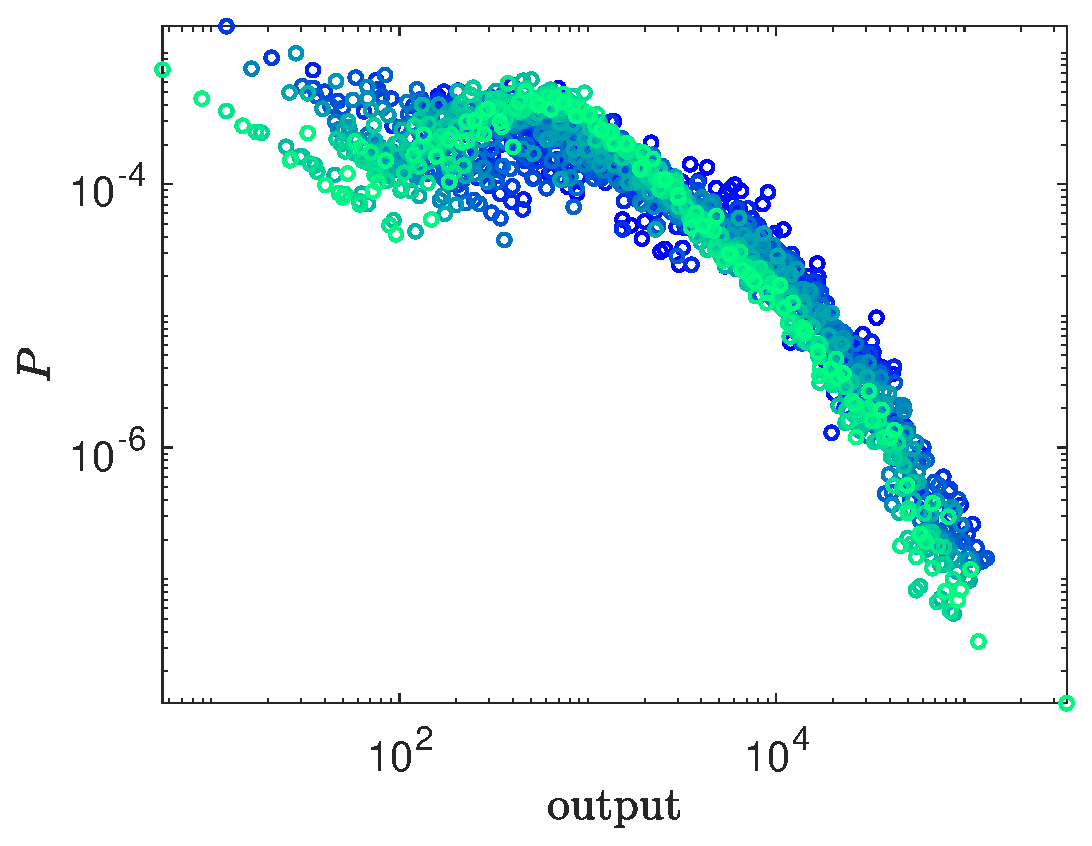
\includegraphics[width=7cm,angle=0]{./Figures/1990_2021_output_distr.eps}
\vspace{0.5cm}
\end{minipage}
\begin{minipage}{0.49\linewidth}
\centering
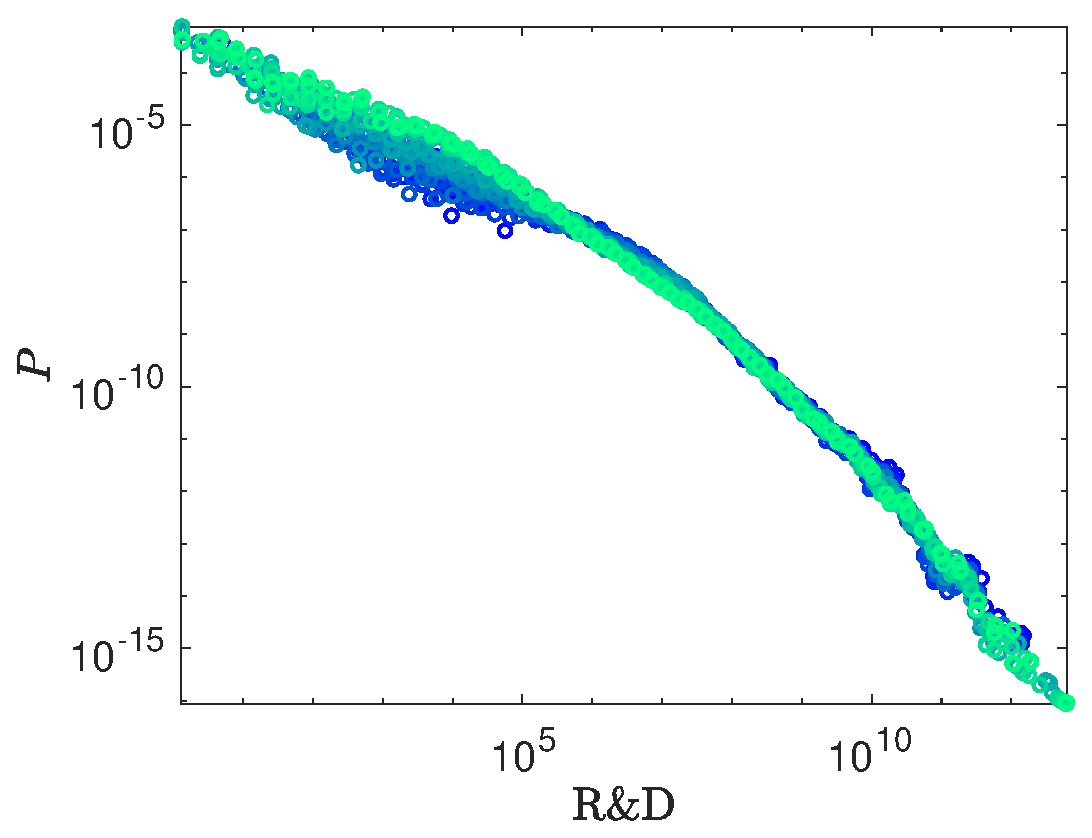
\includegraphics[width=7cm,angle=0]{./Figures/1990_2021_rnd_distr.eps}
\end{minipage}
\begin{minipage}{0.49\linewidth}
\centering
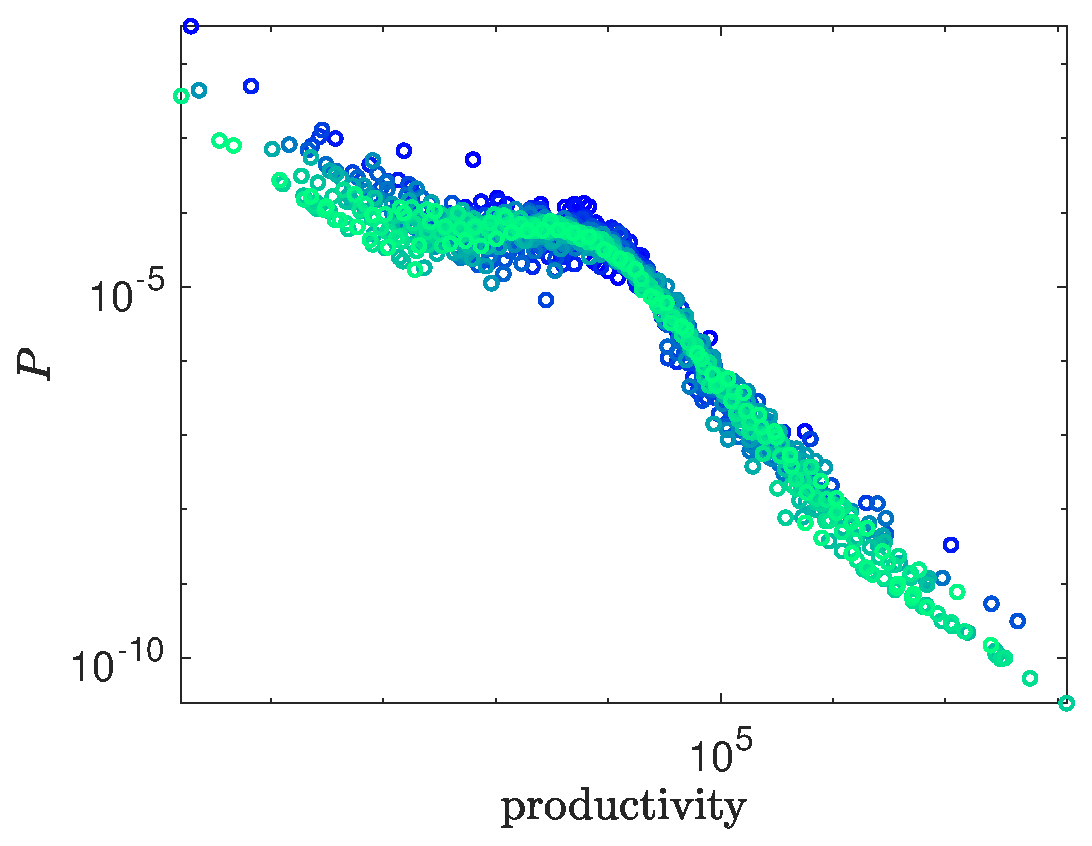
\includegraphics[width=7cm,angle=0]{./Figures/1990_2021_prod_distr.eps}
\end{minipage}
\end{minipage}
%\hspace{-2.5cm}
\begin{minipage}{0.05\linewidth}
\definecolor{col1}{rgb}{0,0,1}
\definecolor{col2}{rgb}{0,0.032258,0.98387}
\definecolor{col3}{rgb}{0,0.064516,0.96774}
\definecolor{col4}{rgb}{0,0.096774,0.95161}
\definecolor{col5}{rgb}{0,0.12903,0.93548}
\definecolor{col6}{rgb}{0,0.16129,0.91935}
\definecolor{col7}{rgb}{0,0.19355,0.90323}
\definecolor{col8}{rgb}{0,0.22581,0.8871}
\definecolor{col9}{rgb}{0,0.25806,0.87097}
\definecolor{col10}{rgb}{0,0.29032,0.85484}
\definecolor{col11}{rgb}{0,0.32258,0.83871}
\definecolor{col12}{rgb}{0,0.35484,0.82258}
\definecolor{col13}{rgb}{0,0.3871,0.80645}
\definecolor{col14}{rgb}{0,0.41935,0.79032}
\definecolor{col15}{rgb}{0,0.45161,0.77419}
\definecolor{col16}{rgb}{0,0.48387,0.75806}
\definecolor{col17}{rgb}{0,0.51613,0.74194}
\definecolor{col18}{rgb}{0,0.54839,0.72581}
\definecolor{col19}{rgb}{0,0.58065,0.70968}
\definecolor{col20}{rgb}{0,0.6129,0.69355}
\definecolor{col21}{rgb}{0,0.64516,0.67742}
\definecolor{col22}{rgb}{0,0.67742,0.66129}
\definecolor{col23}{rgb}{0,0.70968,0.64516}
\definecolor{col24}{rgb}{0,0.74194,0.62903}
\definecolor{col25}{rgb}{0,0.77419,0.6129}
\definecolor{col26}{rgb}{0,0.80645,0.59677}
\definecolor{col27}{rgb}{0,0.83871,0.58065}
\definecolor{col28}{rgb}{0,0.87097,0.56452}
\definecolor{col29}{rgb}{0,0.90323,0.54839}
\definecolor{col30}{rgb}{0,0.93548,0.53226}
\definecolor{col31}{rgb}{0,0.96774,0.51613}
\definecolor{col32}{rgb}{0,1,0.5}
\colorbox{col1!50}{1990} \\
%\colorbox{col2!50}{1991} \\
\colorbox{col3!50}{1992} \\
%\colorbox{col4!50}{1993} \\
\colorbox{col5!50}{1994} \\
%\colorbox{col6!50}{1995} \\
\colorbox{col7!50}{1996} \\
%\colorbox{col8!50}{1997} \\
\colorbox{col9!50}{1998} \\
%\colorbox{col10!50}{1999} \\
\colorbox{col11!50}{2000} \\
%\colorbox{col12!50}{2001} \\
\colorbox{col13!50}{2002} \\
%\colorbox{col14!50}{2003} \\
\colorbox{col15!50}{2004} \\
%\colorbox{col16!50}{2005} \\
\colorbox{col17!50}{2006} \\
%\colorbox{col18!50}{2007} \\
\colorbox{col19!50}{2008} \\
%\colorbox{col20!50}{2009} \\
\colorbox{col21!50}{2010} \\
%\colorbox{col22!50}{2011} \\
\colorbox{col23!50}{2012} \\
%\colorbox{col24!50}{2013} \\
\colorbox{col25!50}{2014} \\
%\colorbox{col26!50}{2015} \\
\colorbox{col27!50}{2016} \\
%\colorbox{col28!50}{2017} \\
\colorbox{col29!50}{2018} \\
%\colorbox{col30!50}{2019} \\
\colorbox{col31!50}{2020} \\
%\colorbox{col32!50}{2021} \\
\end{minipage}
\caption{The sales distribution, output distribution, R\&D expenditures distribution, and the productivity distribution, across different years shown by using a logarithmic binning of the data \citep[][]{McManus1987}.}
\label{fig:balance-sheet-distributions}
\end{figure}

Moreover, Figure \ref{fig:correlations} shows a correlation scatter plot for
sales, output, R\&D expenditures and productivity. All are highly
correlated except for employment and productivity.
\begin{figure}[tbp]
\centering
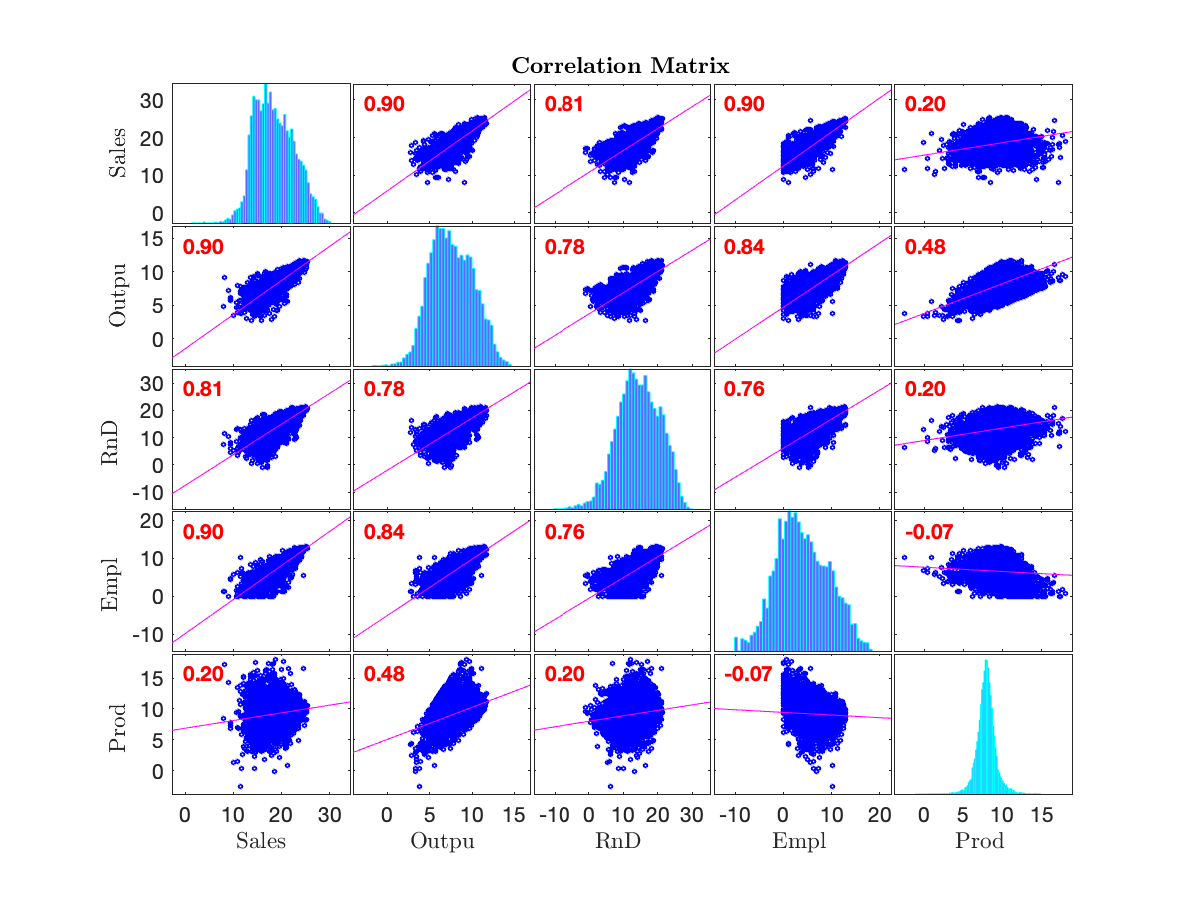
\includegraphics[width=15cm,angle=0]{./Figures/1990_2021_correlations.eps}
\caption{Correlation scatter plot for sales, output, productivity, R\&D expenditures, employment
and productivity at the firm level for the stacked data cross the years 1990 to 2021.}
\label{fig:correlations}
\end{figure}
%%Correlations sales: 1, 0.69968, 0.5403, 0.53018
%%Correlations R\&D: 0.69968, 1, 0.2982, 0.55844
%%Correlations productivity  : 0.5403, 0.2982, 1, 0.22449
%%Correlations num. patents     : 0.53018, 0.55844, 0.22449, 1
%}

%%%%%%%%%%%%%%%%%%%%%%%%%%%%%%%%%%%%%%%%%%%%%%%%%%%%%%%%%
\subsection{\protect Geographic Location and Distance}
\label{sec:locations}
%%%%%%%%%%%%%%%%%%%%%%%%%%%%%%%%%%%%%%%%%%%%%%%%%%%%%%%%%
The number of firms in each country is shown in Figures \ref{fig:countries_firms_count_pie_chart}, \ref{fig:countries_firms_count_map} and  \ref{fig:countries_firms_count_map}, respectively, while Table \ref{tab:countries} shows the 25 countries with
the largest numbers of firms. The dominant role of the U.S. with 7,758
firms making up $52.61\%$ of the total number of firms is
clearly visible. The second largest country in terms of R\&D collaborating firms 
is the United Kingdom with 967 firms, which comprises $6.56\%$ of all collaborations, which is far below the corresponding number for the US. This unequal distribution across countries is a persistent phenomenon across time, as illustrated in Figure \ref{fig:top5-countries}.

\begin{figure}[tbp]
\centering
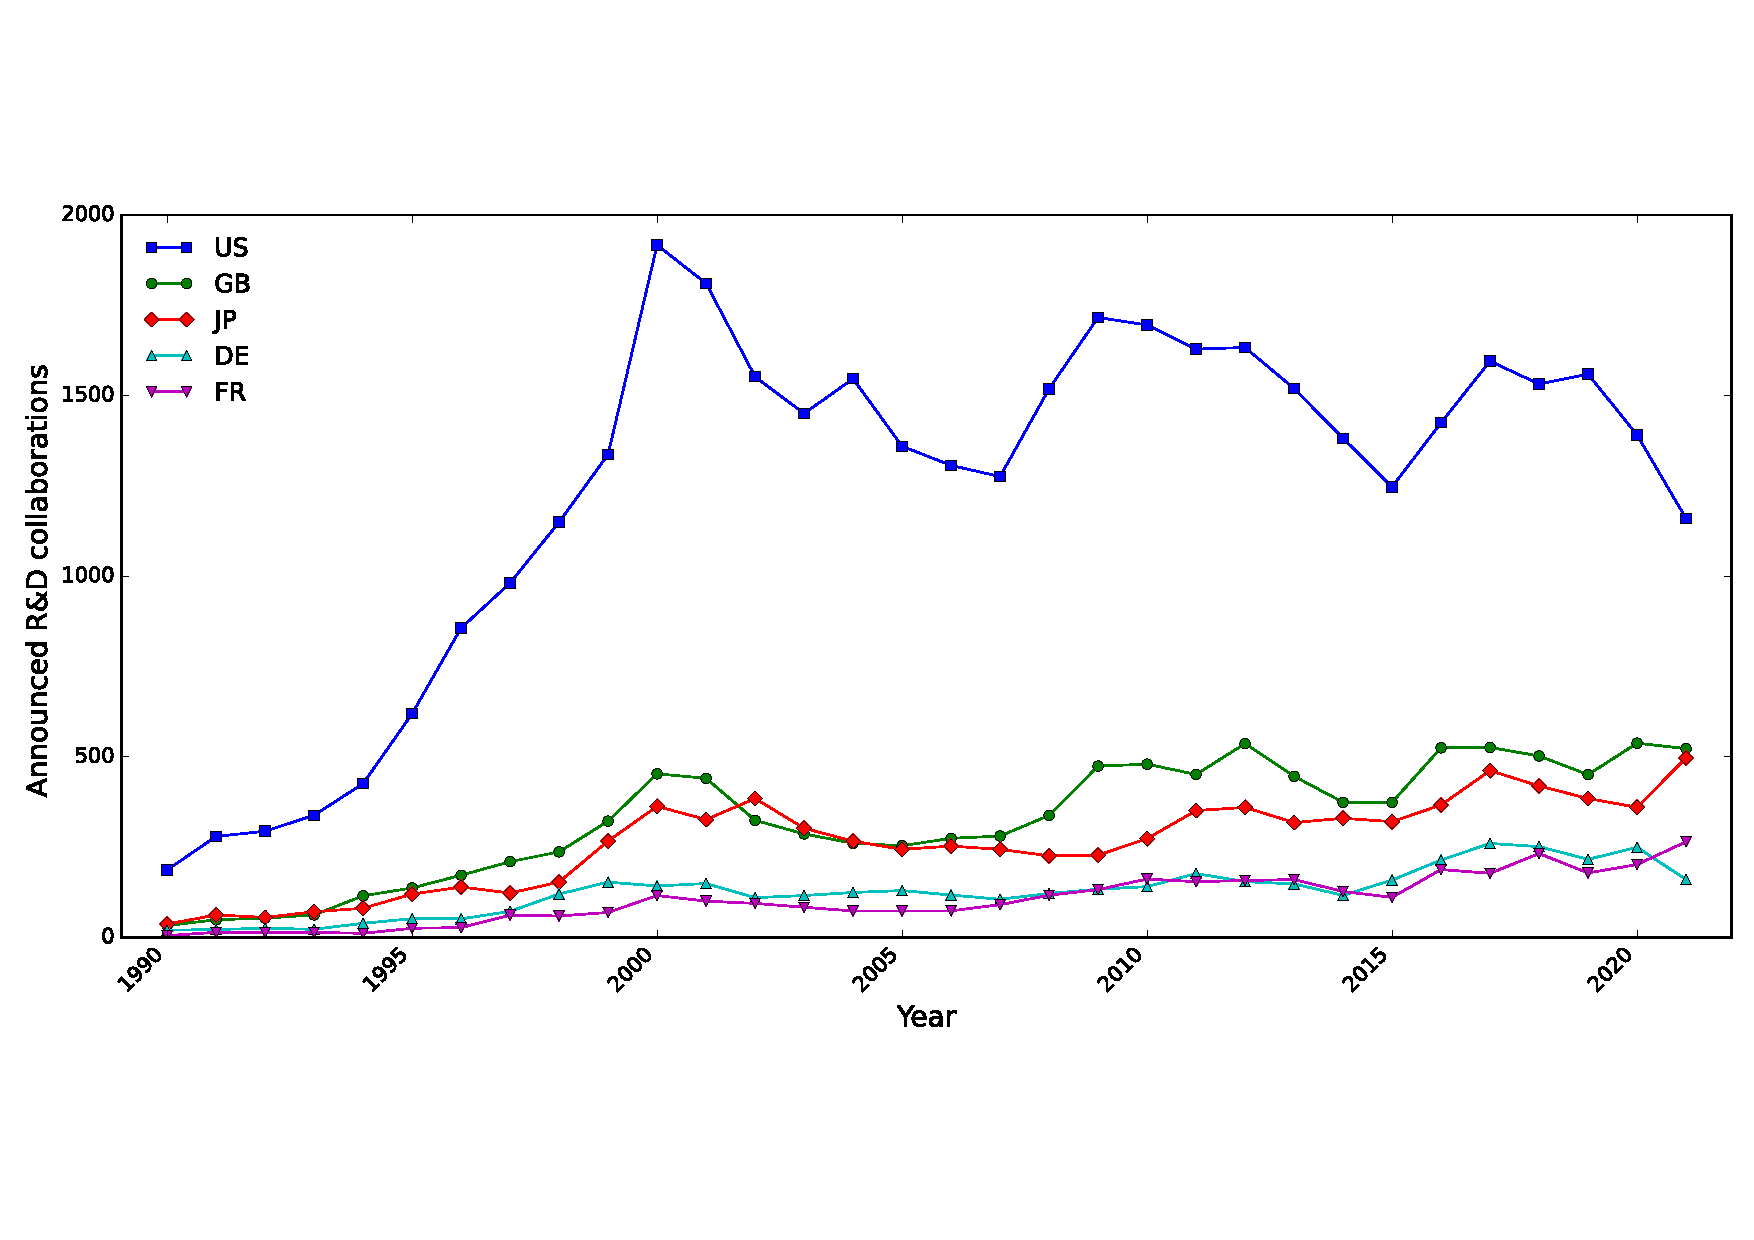
\includegraphics[width=\textwidth,angle=0]{./Figures/rnd_countries_over_time.pdf} 
\caption{R\&D collaborations in the top 5 countries over time. Note that data for 2021 is only partially available (until August 2021).}
\label{fig:top5-countries}
\end{figure}

\begin{figure}[tbp]
\centering
\centerline{
\scalebox{0.45}{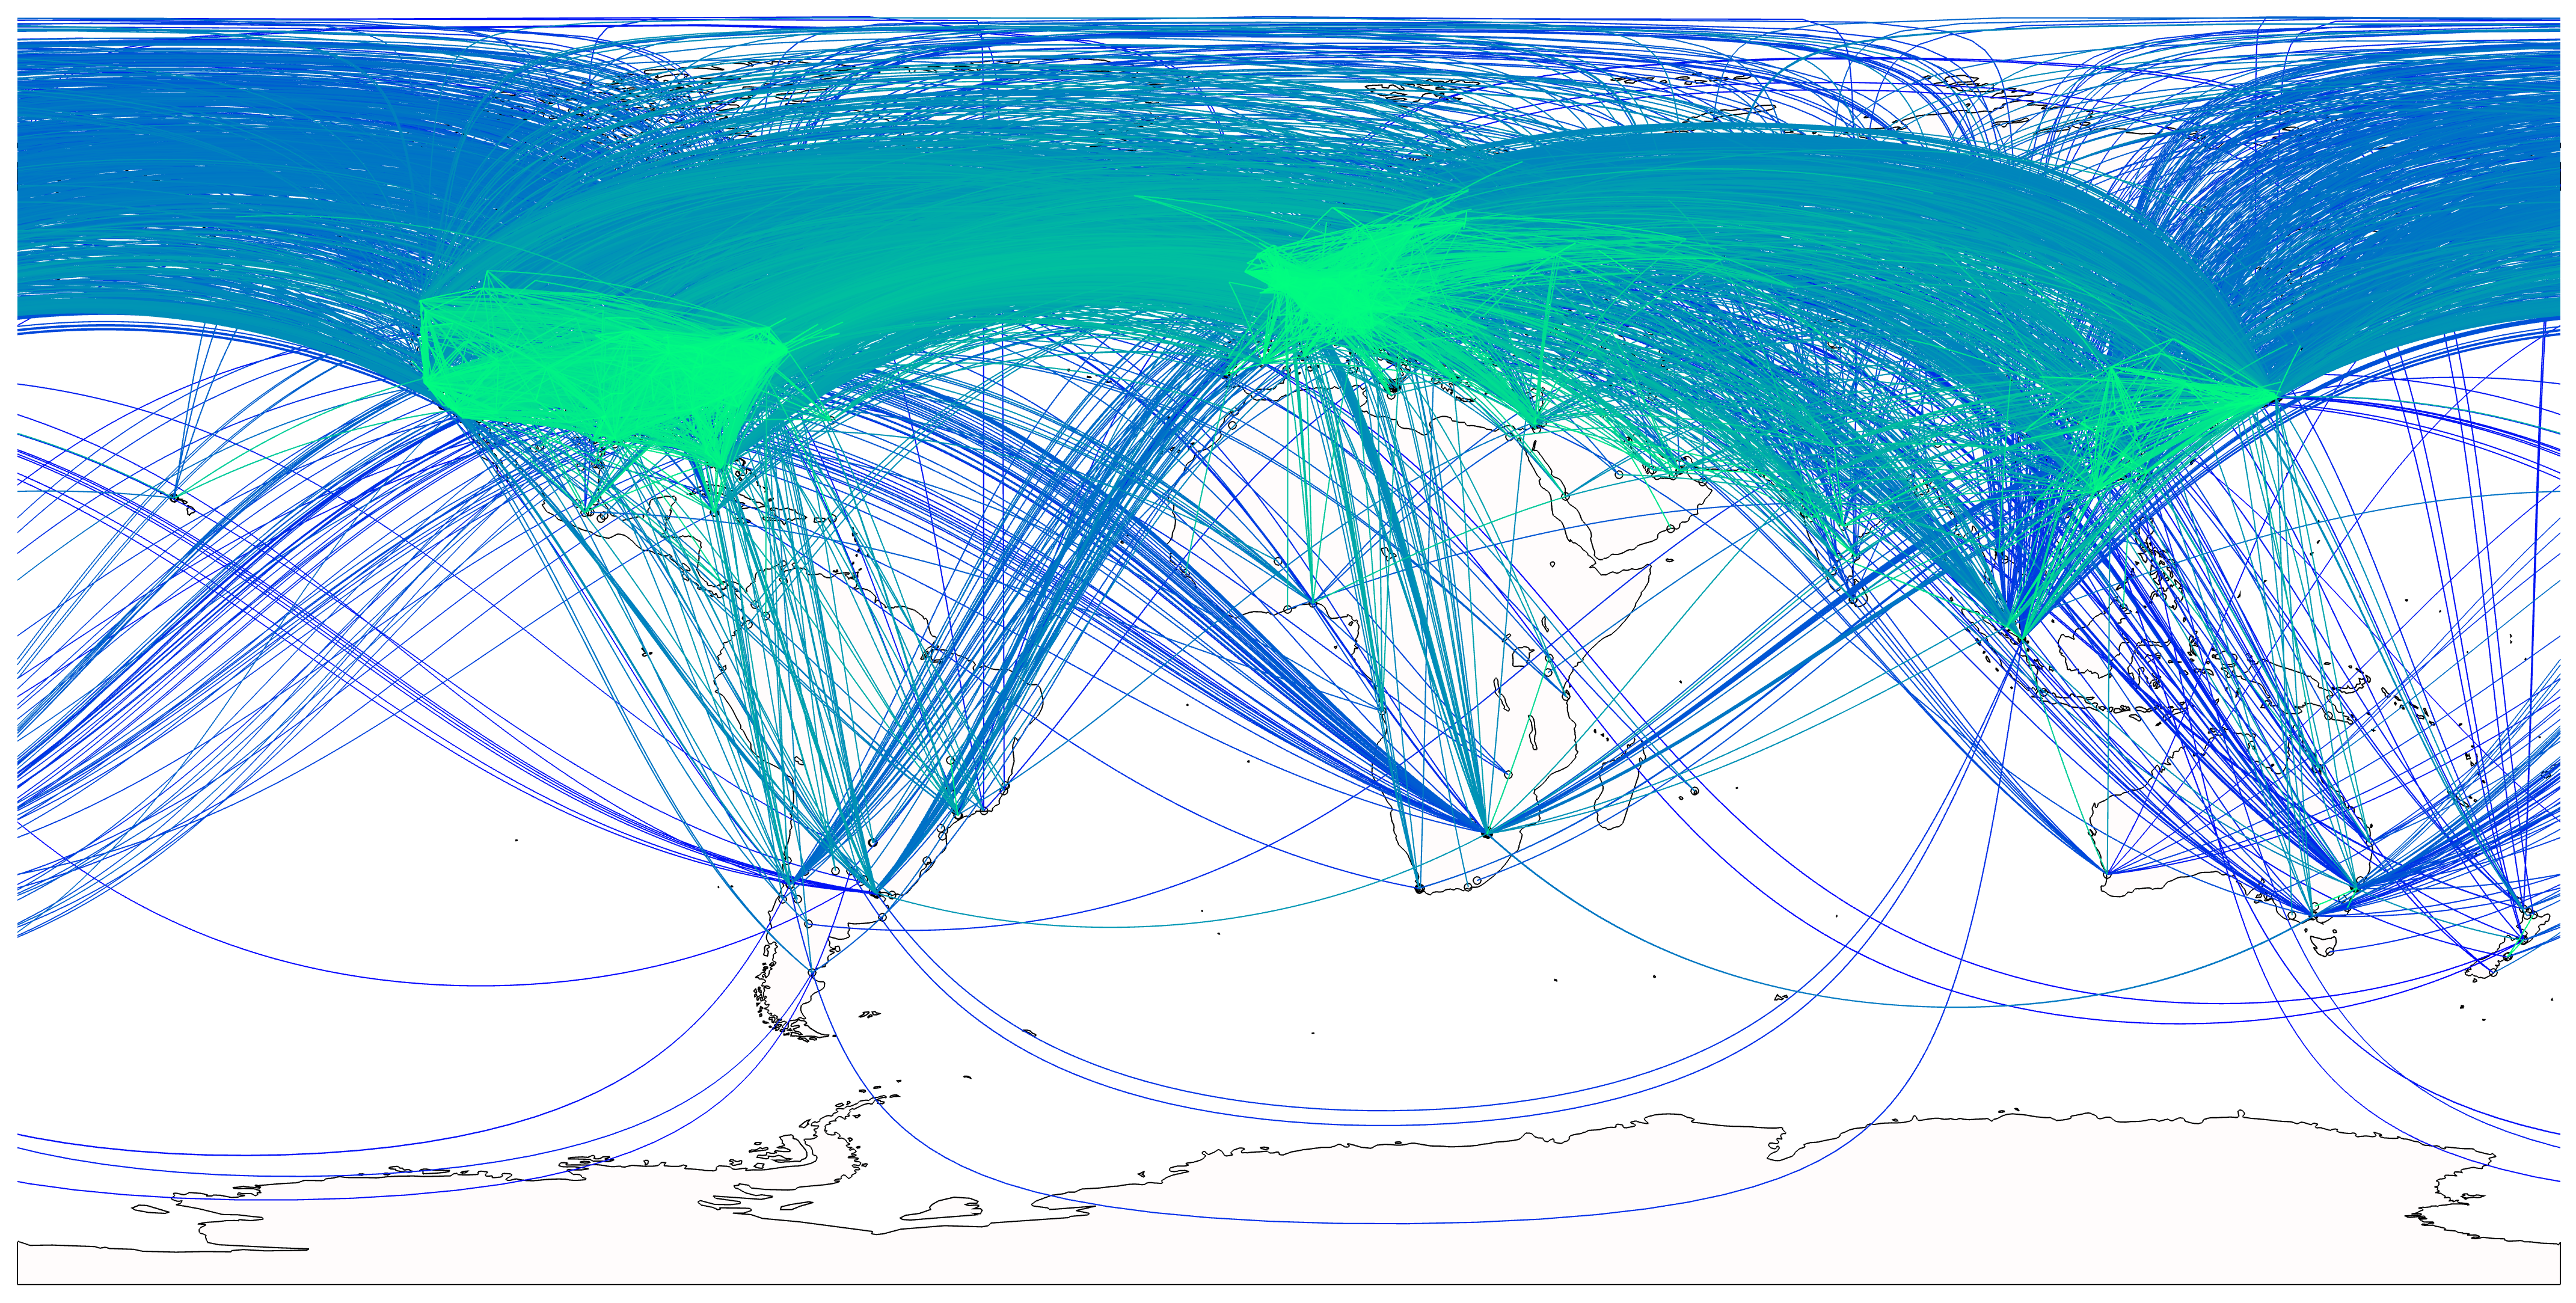
\includegraphics{./Figures/2021_network_tot_world_map.png}}}
\caption{The locations (at the city level) and collaborations of the firms accumulated over all years (1980 to 2021).}
\label{fig:alliances_world_map}
\end{figure}

\begin{figure}[tbp]
%\vspace{-2cm}
\centering
\begin{center}
%\centerline{
%\hspace{5cm}
\scalebox{1}{
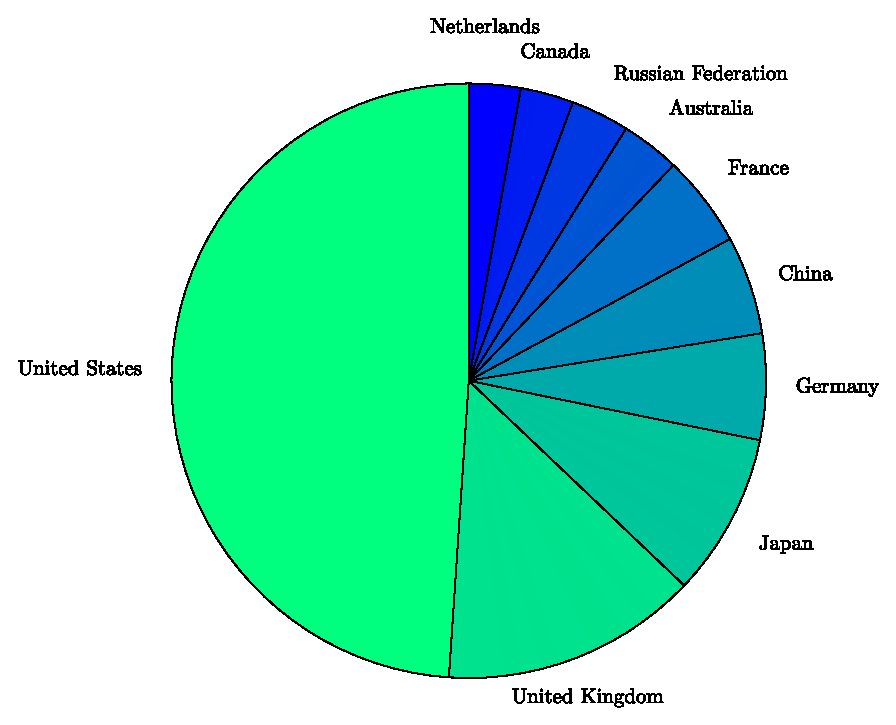
\includegraphics[width=10cm,angle=0]{./Figures/countries_distr.eps}
}%}
\end{center}
%\vspace{1.5cm}
\caption{Pie chart illustrating the relative number of firms across countries.}
\label{fig:countries_firms_count_pie_chart}
\end{figure}

\begin{table}[tpb]
\centering
{\footnotesize
\begin{threeparttable}
\caption{The 25 countries with the largest numbers of firms.}
\label{tab:countries}
\begin{tabular}{lcccc}
%ccccccc
\toprule
Country Name & Code & $\#$ firms &  $\%$ of tot. & Rank
\\
\midrule
United States & 	 USA & 	 4113 & 	 38.31 & 	 1 \\ 
United Kingdom & 	 GBR & 	 1174 & 	 10.94 & 	 2 \\ 
Japan & 	 JPN & 	 747 & 	 6.96 & 	 3 \\ 
Germany & 	 DEU & 	 485 & 	 4.52 & 	 4 \\ 
China & 	 CHN & 	 450 & 	 4.19 & 	 5 \\ 
France & 	 FRA & 	 420 & 	 3.91 & 	 6 \\ 
Australia & 	 AUS & 	 270 & 	 2.51 & 	 7 \\ 
Russia & 	RUS  & 	 267 & 	 2.49 & 	  8 \\ 
Canada & 	 CAN & 	 243 & 	 2.26 & 	 9 \\ 
Netherlands & 	 NLD & 	 236 & 	 2.20 & 	 10 \\ 
Italy & 	 ITA & 	 219 & 	 2.04 & 	 11 \\ 
India & 	 IND & 	 193 & 	 1.80 & 	 12 \\ 
Hong Kong & 	 HKG & 	 173 & 	 1.61 & 	 13 \\ 
Korea & 	KOR  & 	 171 & 	 1.59 & 	  14 \\ 
Sweden & 	 SWE & 	 129 & 	 1.20 & 	 15 \\ 
Switzerland & 	 CHE & 	 117 & 	 1.09 & 	 16 \\ 
Singapore & 	 SGP & 	 115 & 	 1.07 & 	 17 \\ 
Belgium & 	 BEL & 	 90 & 	 0.84 & 	 18 \\ 
Taiwan & 	 TWN & 	 90 & 	 0.84 & 	 19 \\ 
Malaysia & 	 MYS & 	 80 & 	 0.75 & 	 20 \\ 
Israel & 	 ISR & 	 79 & 	 0.74 & 	 21 \\ 
Finland & 	 FIN & 	 63 & 	 0.59 & 	 22 \\ 
Ireland & 	 IRL & 	 57 & 	 0.53 & 	 23 \\ 
South Africa & 	 ZAF & 	 53 & 	 0.49 & 	 24 \\ 
Poland & 	 POL & 	 48 & 	 0.45 & 	 25 \\ 
\midrule
\bottomrule
\end{tabular}
%\begin{tablenotes}[flushleft]
%\item
%\end{tablenotes}
\end{threeparttable}
}
\end{table}

\begin{figure}[tbp]
\centering
\begin{minipage}{\linewidth}
\centering
%\footnotesize
\definecolor{col1}{rgb}{0,1,0.5}
\definecolor{col2}{rgb}{0,0.88889,0.55556}
\definecolor{col3}{rgb}{0,0.77778,0.61111}
\definecolor{col4}{rgb}{0,0.66667,0.66667}
\definecolor{col5}{rgb}{0,0.55556,0.72222}
\definecolor{col6}{rgb}{0,0.44444,0.77778}
\definecolor{col7}{rgb}{0,0.33333,0.83333}
\definecolor{col8}{rgb}{0,0.22222,0.88889}
\definecolor{col9}{rgb}{0,0.11111,0.94444}
\definecolor{col10}{rgb}{0,0,1}
%\hspace{-5cm}
\makebox{\footnotesize
\colorbox{col1!50}{[0,1]} %\\
\colorbox{col2!50}{[1,2]} %\\
\colorbox{col3!50}{[2,8]} %\\
\colorbox{col4!50}{[8,22]} %\\
\colorbox{col5!50}{[22,64]} %\\
\colorbox{col6!50}{[64,181]} %\\
\colorbox{col7!50}{[181,513]} %\\
\colorbox{col8!50}{[513,1453]} %\\
\colorbox{col9!50}{[1453,4113]} %\\
}
\end{minipage}
\begin{minipage}{\linewidth}
\centerline{\scalebox{0.9}{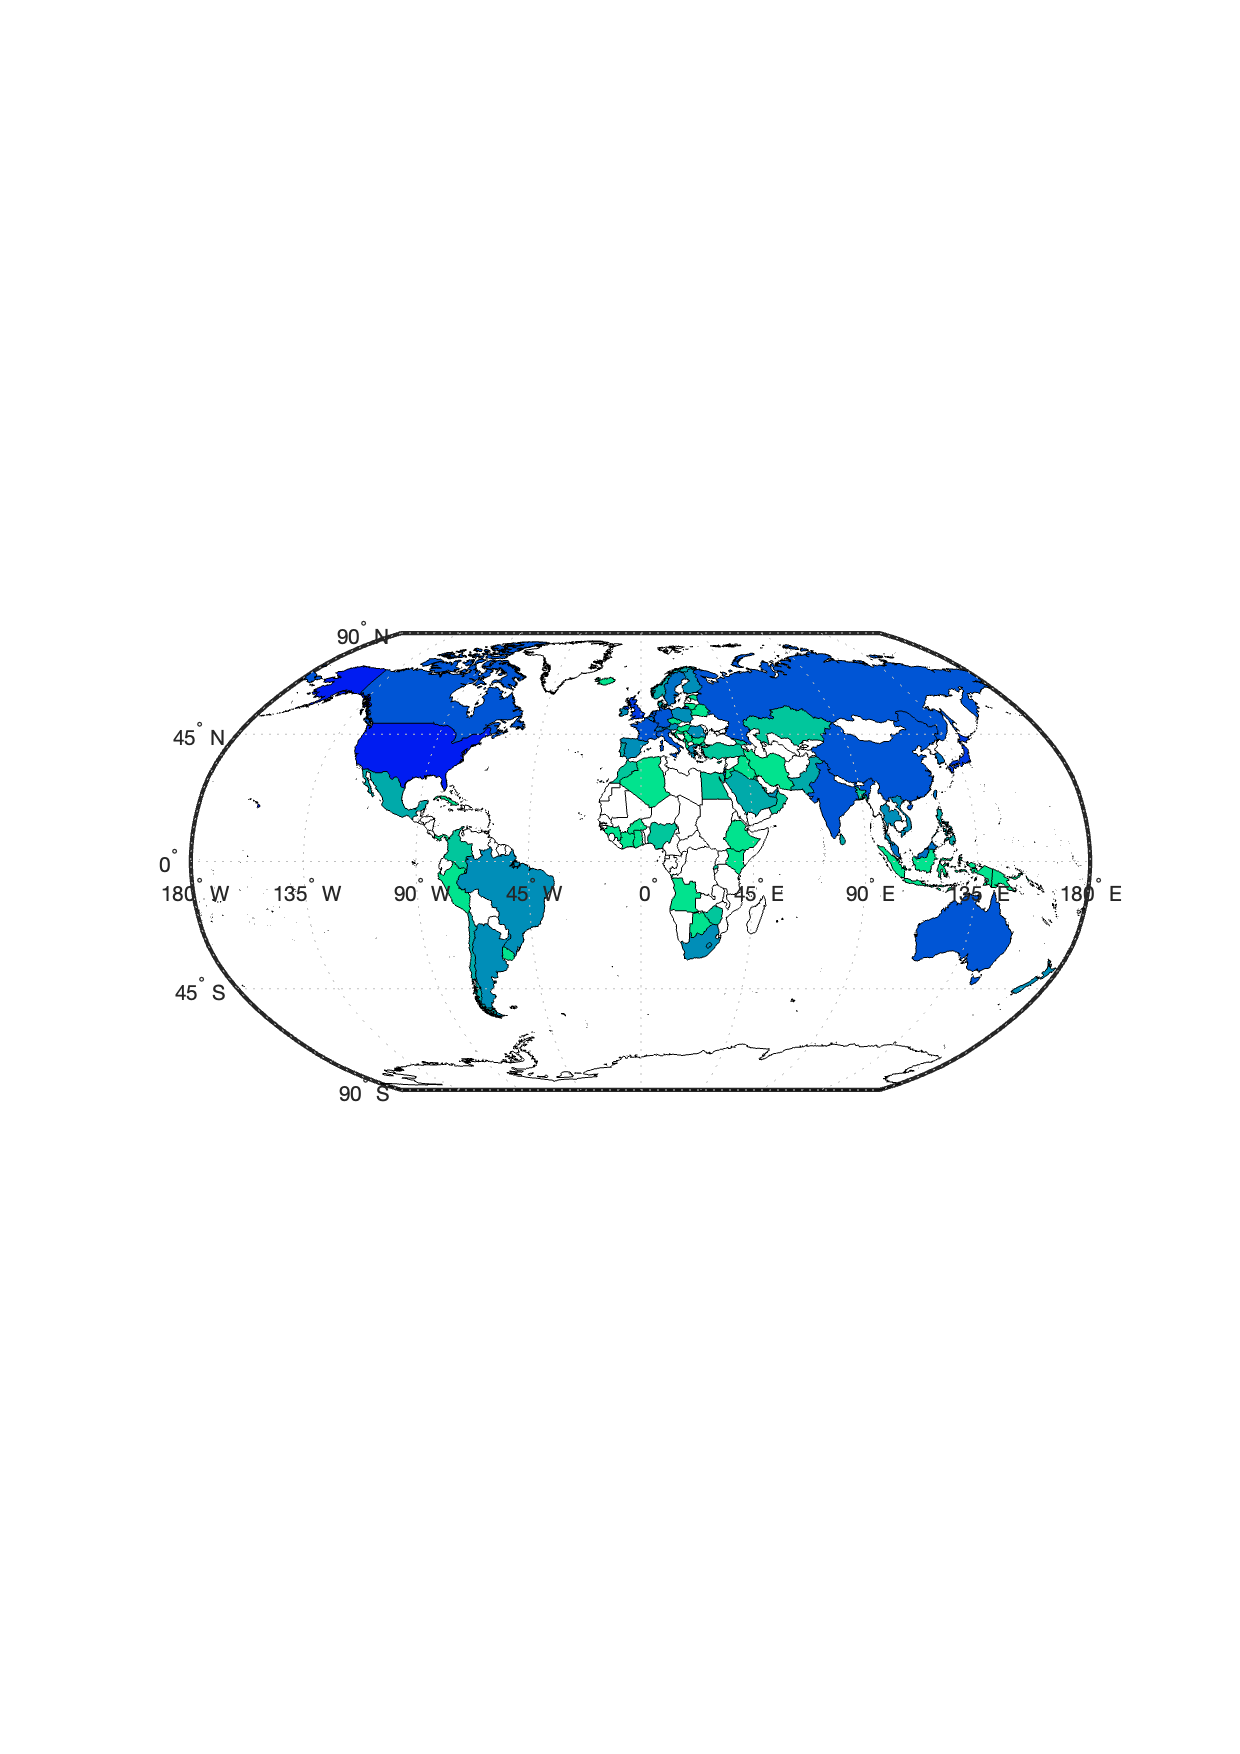
\includegraphics{./Figures/countries_num_firms.pdf}}}
%\vspace{-1cm}
\end{minipage}
\caption{The number of firms in each country in the data sample.}
\label{fig:countries_firms_count_map}
\end{figure}

In order to determine the precise locations of the firms in our
data we have further added the longitude and latitude coordinates associated with the city of residence of each firm. Among the matched cities in our dataset $93.67\%$ could be geo-localized using ArcGIS \citep[see e.g.,][]{Dell2009} and the Google Maps Geocoding API. We then used Vincenty's algorithm to compute the distances between pairs of
geo-localized firms \citep{Vincenty1975}. %The mean distance between collaborating firms is $5,227$ km. 
The distance distribution, $P(d)$, across collaborating firms is shown in Figure \ref{fig:dist-mean-distribution}, while Figure \ref{fig:alliances_world_map} shows the locations (at the city level) and collaborations of the firms in the database. The distance distribution, $P(d) $, is heavily skewed. We find that R\&D collaborations tend to be more likely between firms that are close, showing that geography matters for R\&D collaborations and this spillovers, in line with previous empirical studies \citep{Lychagin2010}. Moreover, Figure \ref{fig:dist-mean-distribution} shows that the distance between R\&D collaborating firms is fluctuating over time.

%\begin{figure}[tbp]
%\centering
%\centerline{
%\scalebox{1.2}{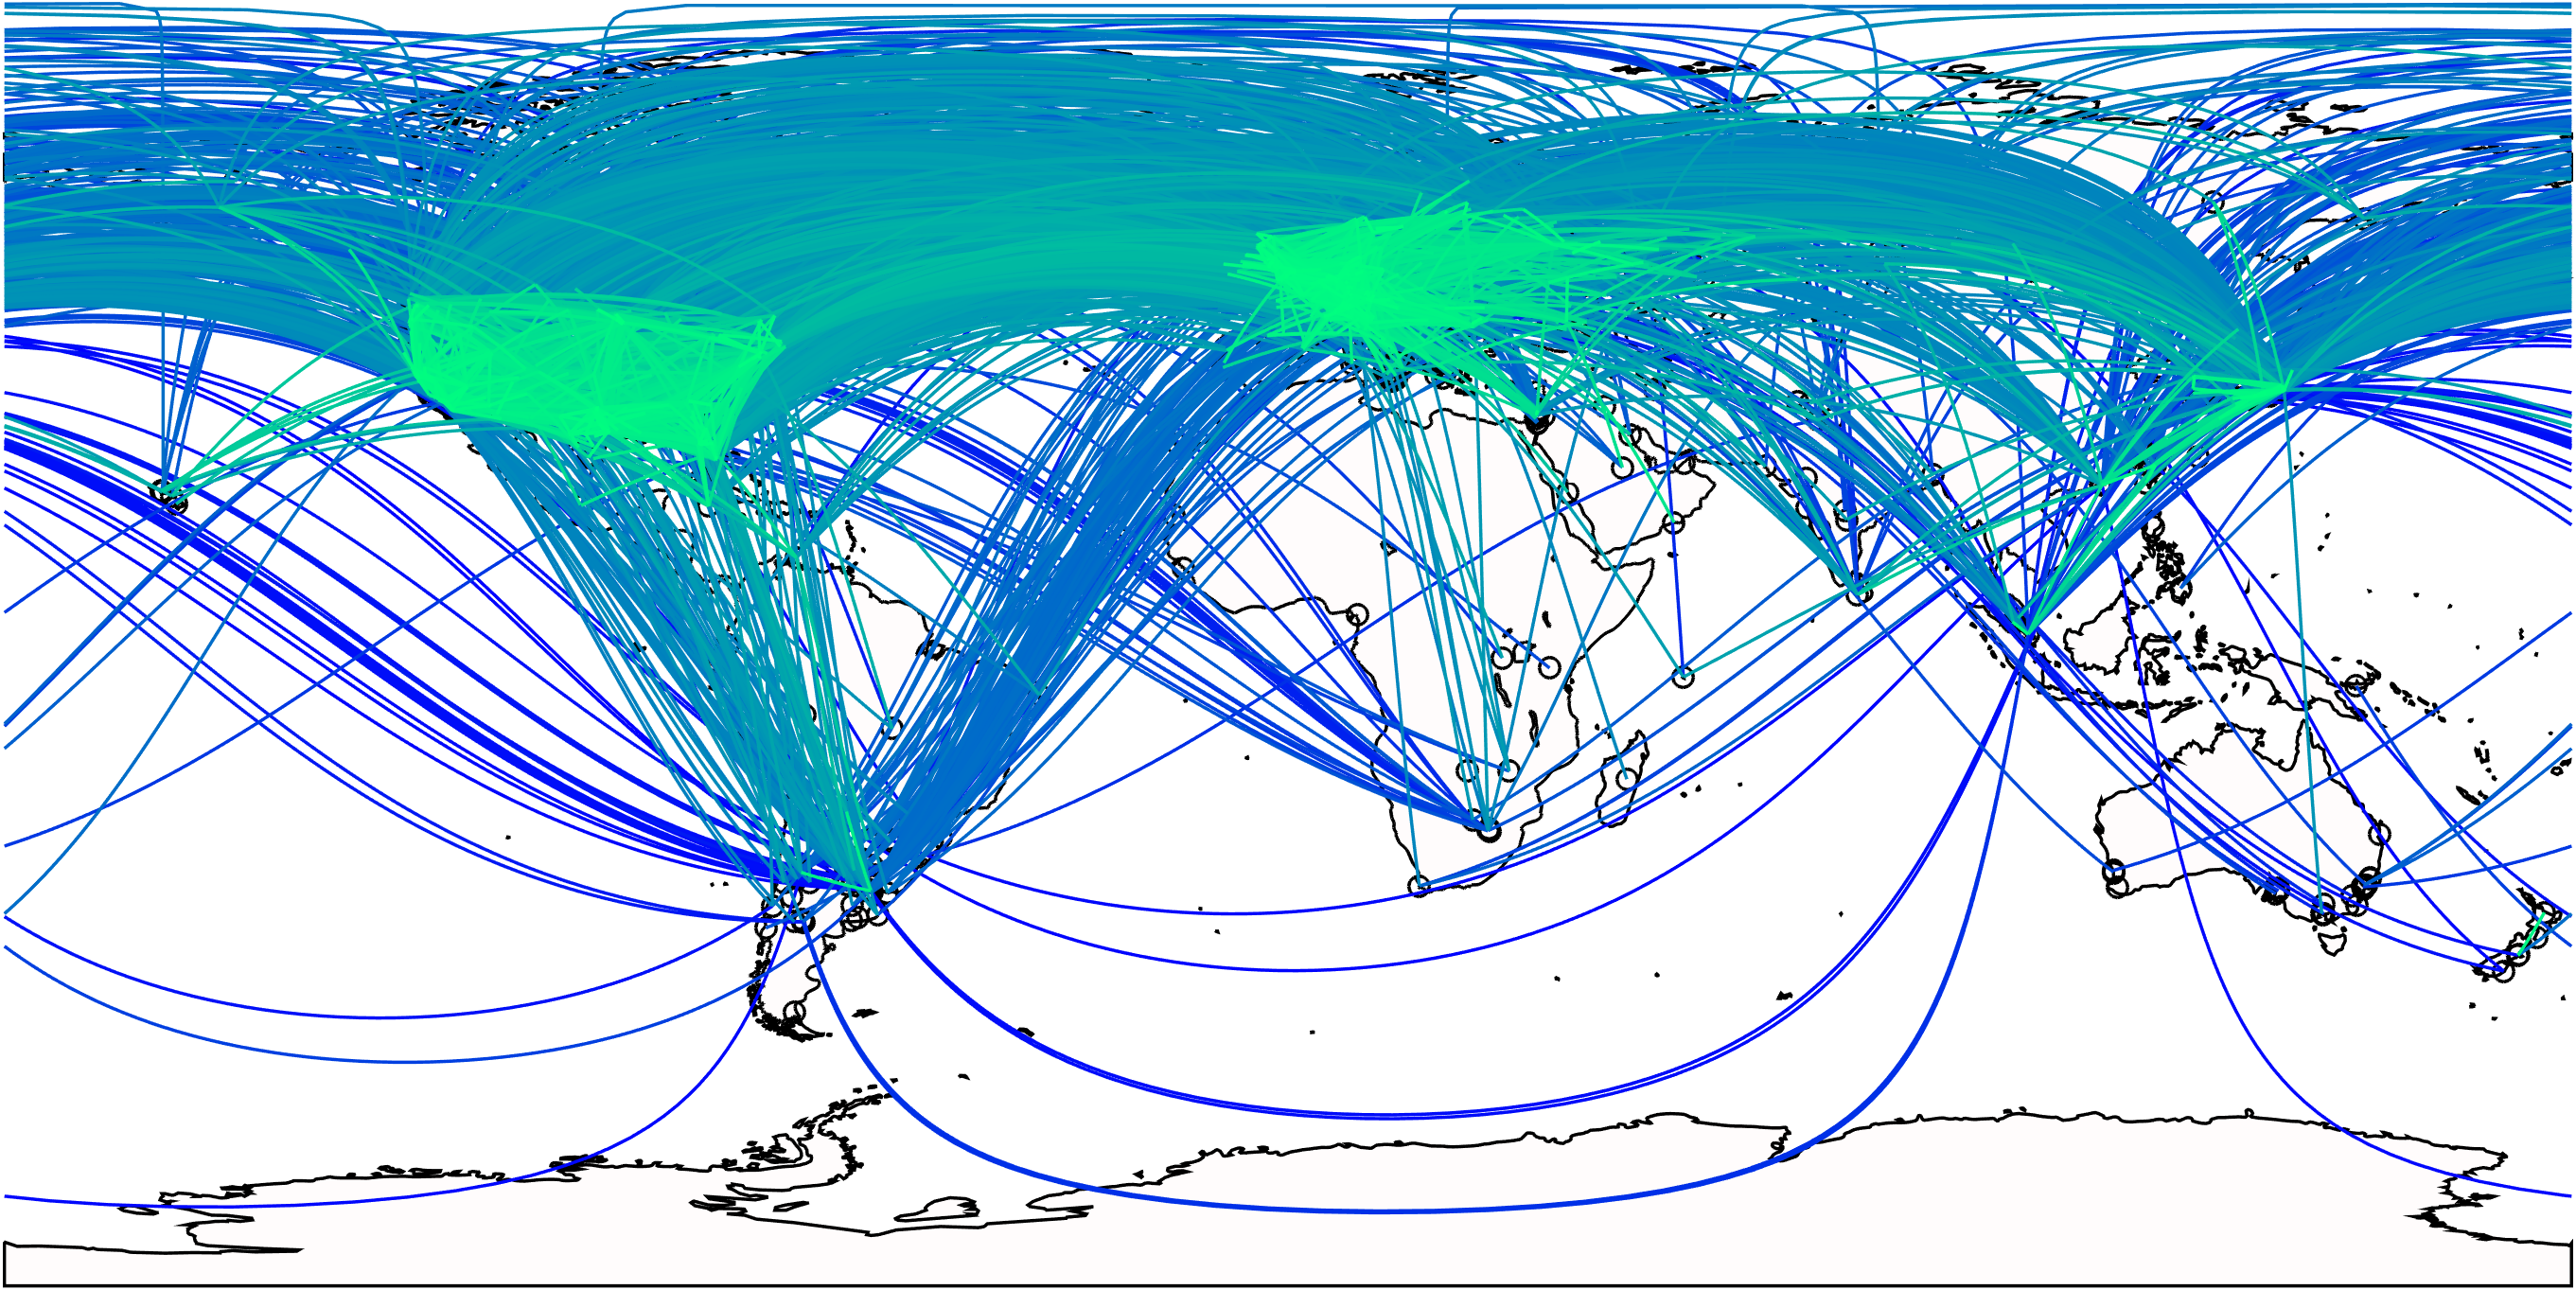
\includegraphics{./Figures/2021_network_tot_world_map_2.png}}}
%\caption{The locations (at the city level) and collaborations of the firms accumulated over all years (1980 to 2021).}
%\label{fig:alliances_world_map}
%\end{figure}

\begin{figure}[tbp]
\begin{minipage}{0.9\linewidth}
\centering
\begin{minipage}{0.49\linewidth}
\centering
\vspace{-0.5cm}
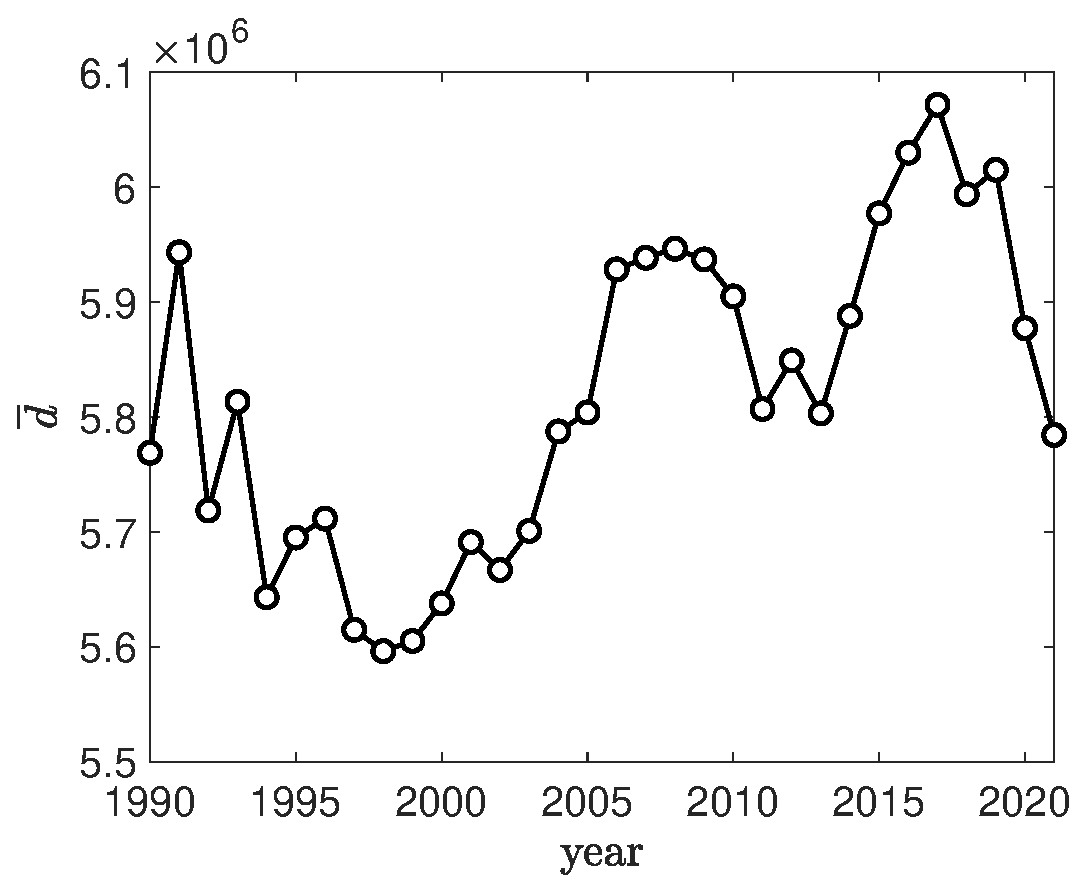
\includegraphics[width=7cm,angle=0]{./Figures/1990_2021_alliance_duration_5_mean_distance.eps}
\end{minipage}
\begin{minipage}{0.49\linewidth}
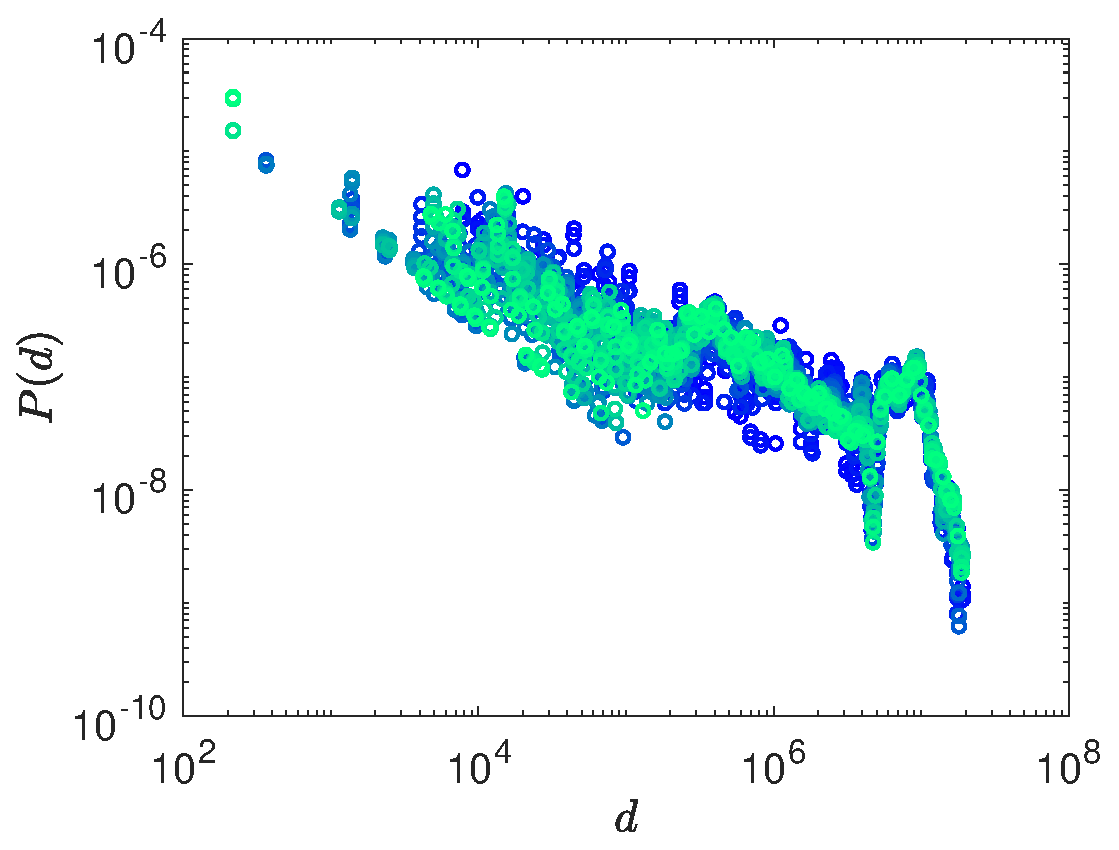
\includegraphics[width=7.5cm,angle=0]{./Figures/1990_2021_alliance_duration_5_distance_distr.eps}
\end{minipage}
\end{minipage}
\hspace{0.5cm}
\begin{minipage}{0.05\linewidth}
\vspace{-0.5cm}
\footnotesize
\definecolor{col1}{rgb}{0,0,1}
\definecolor{col2}{rgb}{0,0.032258,0.98387}
\definecolor{col3}{rgb}{0,0.064516,0.96774}
\definecolor{col4}{rgb}{0,0.096774,0.95161}
\definecolor{col5}{rgb}{0,0.12903,0.93548}
\definecolor{col6}{rgb}{0,0.16129,0.91935}
\definecolor{col7}{rgb}{0,0.19355,0.90323}
\definecolor{col8}{rgb}{0,0.22581,0.8871}
\definecolor{col9}{rgb}{0,0.25806,0.87097}
\definecolor{col10}{rgb}{0,0.29032,0.85484}
\definecolor{col11}{rgb}{0,0.32258,0.83871}
\definecolor{col12}{rgb}{0,0.35484,0.82258}
\definecolor{col13}{rgb}{0,0.3871,0.80645}
\definecolor{col14}{rgb}{0,0.41935,0.79032}
\definecolor{col15}{rgb}{0,0.45161,0.77419}
\definecolor{col16}{rgb}{0,0.48387,0.75806}
\definecolor{col17}{rgb}{0,0.51613,0.74194}
\definecolor{col18}{rgb}{0,0.54839,0.72581}
\definecolor{col19}{rgb}{0,0.58065,0.70968}
\definecolor{col20}{rgb}{0,0.6129,0.69355}
\definecolor{col21}{rgb}{0,0.64516,0.67742}
\definecolor{col22}{rgb}{0,0.67742,0.66129}
\definecolor{col23}{rgb}{0,0.70968,0.64516}
\definecolor{col24}{rgb}{0,0.74194,0.62903}
\definecolor{col25}{rgb}{0,0.77419,0.6129}
\definecolor{col26}{rgb}{0,0.80645,0.59677}
\definecolor{col27}{rgb}{0,0.83871,0.58065}
\definecolor{col28}{rgb}{0,0.87097,0.56452}
\definecolor{col29}{rgb}{0,0.90323,0.54839}
\definecolor{col30}{rgb}{0,0.93548,0.53226}
\definecolor{col31}{rgb}{0,0.96774,0.51613}
\definecolor{col32}{rgb}{0,1,0.5}
\colorbox{col1!50}{1990} \\
%\colorbox{col2!50}{1991} \\
%\colorbox{col3!50}{1992} \\
%\colorbox{col4!50}{1993} \\
%\colorbox{col5!50}{1994} \\
\colorbox{col6!50}{1995} \\
%\colorbox{col7!50}{1996} \\
%\colorbox{col8!50}{1997} \\
%\colorbox{col9!50}{1998} \\
%\colorbox{col10!50}{1999} \\
\colorbox{col11!50}{2000} \\
%\colorbox{col12!50}{2001} \\
%\colorbox{col13!50}{2002} \\
%\colorbox{col14!50}{2003} \\
%\colorbox{col15!50}{2004} \\
\colorbox{col16!50}{2005} \\
%\colorbox{col17!50}{2006} \\
%\colorbox{col18!50}{2007} \\
%\colorbox{col19!50}{2008} \\
%\colorbox{col20!50}{2009} \\
\colorbox{col21!50}{2010} \\
%\colorbox{col22!50}{2011} \\
%\colorbox{col23!50}{2012} \\
%\colorbox{col24!50}{2013} \\
%\colorbox{col25!50}{2014} \\
\colorbox{col26!50}{2015} \\
%\colorbox{col27!50}{2016} \\
%\colorbox{col28!50}{2017} \\
%\colorbox{col29!50}{2018} \\
%\colorbox{col30!50}{2019} \\
\colorbox{col31!50}{2020} \\
%\colorbox{col32!50}{2021} \\
\end{minipage}
\caption{(Left panel) The average distance between collaborating firms. (Right panel) The distance distribution, $P(d)$, across
collaborating firms.}
\label{fig:dist-mean-distribution}
\end{figure}

%Mean distance is ... m
%Distance variance is ... m
%Distance std is ... m

% %%%%%%%%%%%%%%%%%%%%%%%%%%%%%%%%%%%%%%%%%%%%%%%%%%%%%%%%%%
% \subsection{Nestedness and Modularity}
% \label{sec:nested-module}
% %%%%%%%%%%%%%%%%%%%%%%%%%%%%%%%%%%%%%%%%%%%%%%%%%%%%%%%%%%
% We can identify clusters -- or so called modules -- of densely connected firms in the network (with only sparser connections across clusters) using the \emph{modularity} algorithm proposed by \citet{Newman2006}. This algorithm seeks a division of the nodes in the network into non-overlapping clusters, where these clusters may be of any size. Such clusters might emerge because of similarities of firms in terms of the industry in which they are operating, technological similarity or geographic proximity (lowering collaboration costs and thus making certain pairs of firms more likely to be connected).

% After having identified these modules we can compute the nestedness of each module (cf. Figure \ref{fig:network-time-series}). The top left panel in Figure \ref{fig:1990_cc_nestedness_modularity_adjacency_matrices} shows the adjacency matrix of the largest connected component of the R\&D network in the year 1990 %(see Fig. \ref{fig:1990_cc_graph}) 
% where the modules identified are indicated with different colors. The top middle and top right panels zoom into the largest modules. The bottom left panel shows the adjacency matrices of each module (sub-network) separately (showing only the first 10 modules with the highest modularity and size), where a (+) indicates that the matrix is statistically significantly nested at the 5\% level \citep{AlmeidaNeto2008}. The solid red line indicates the isocline (that is, a curve that divides the ones from the zeros of a perfectly nested matrix of the same size and connectivity). The bottom right panel shows the nestedness coefficients, $C_n$, of these 10 modules (sorted by $C_n$). Figures \ref{fig:2000_cc_nestedness_modularity_adjacency_matrices}, \ref{fig:2010_cc_nestedness_modularity_adjacency_matrices} and \ref{fig:2020_cc_nestedness_modularity_adjacency_matrices} show the same information but for the years 2000, 2010 and 2020. We observe that all modules are highly nested, and most modules considered are also significantly nested, in particular, in the years 2000, 2010 and 2020. This is consistent with the bottom right panel in Figure \ref{fig:network-time-series} showing the evolution over time of the nestedness coefficient, $C_n$, with a nestedness coefficient close to one in the years after 2000.

% \begin{figure}
% \begin{center}
% Year: 1990
% \end{center}
% \begin{minipage}{\linewidth}
% \centering
% 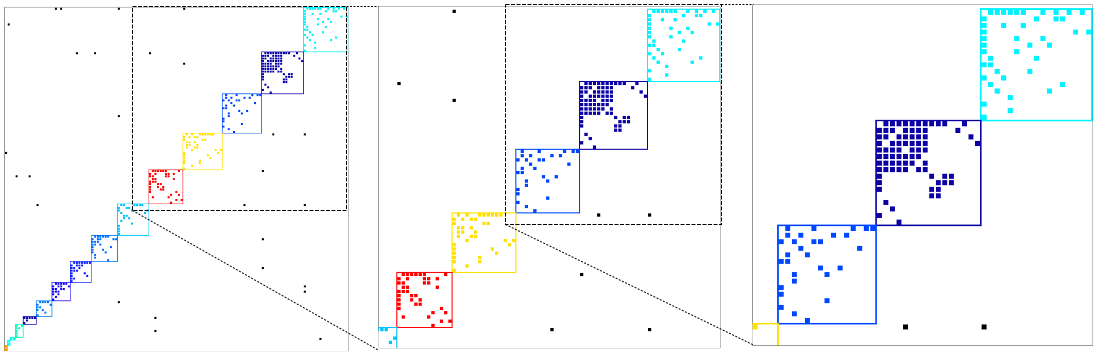
\includegraphics[width=\textwidth]{./Figures/1990_cc_modularity_adjacency_matrix_1_2_3.png}
% \end{minipage}
% \begin{minipage}{\linewidth}
% ${}$
% \end{minipage}
% \begin{minipage}{0.45\linewidth}
% \centering
% 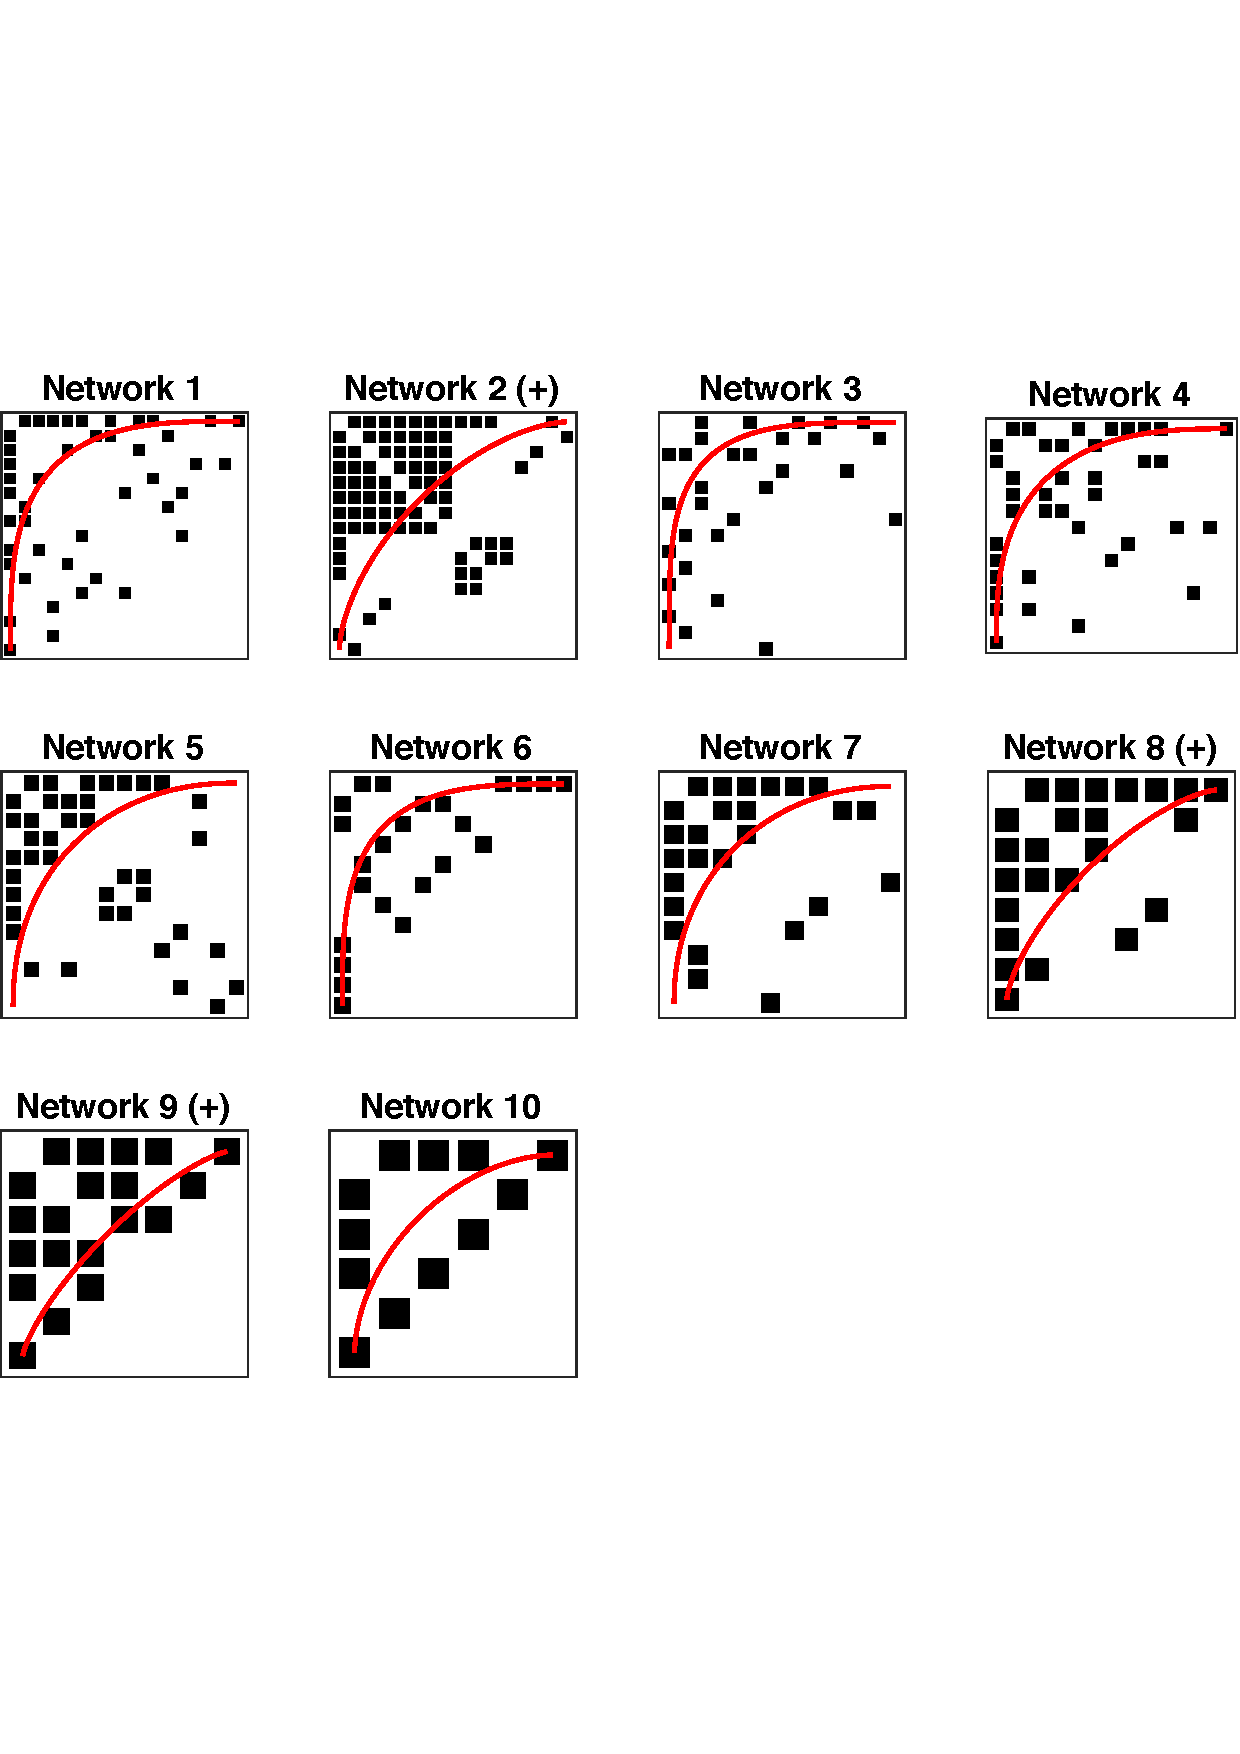
\includegraphics[width=\textwidth]{./Figures/1990_cc_adjacency_matrices.pdf}
% \end{minipage}
% \begin{minipage}{0.1\linewidth}
% \end{minipage}
% \begin{minipage}{0.3725\linewidth}
% \centering
% 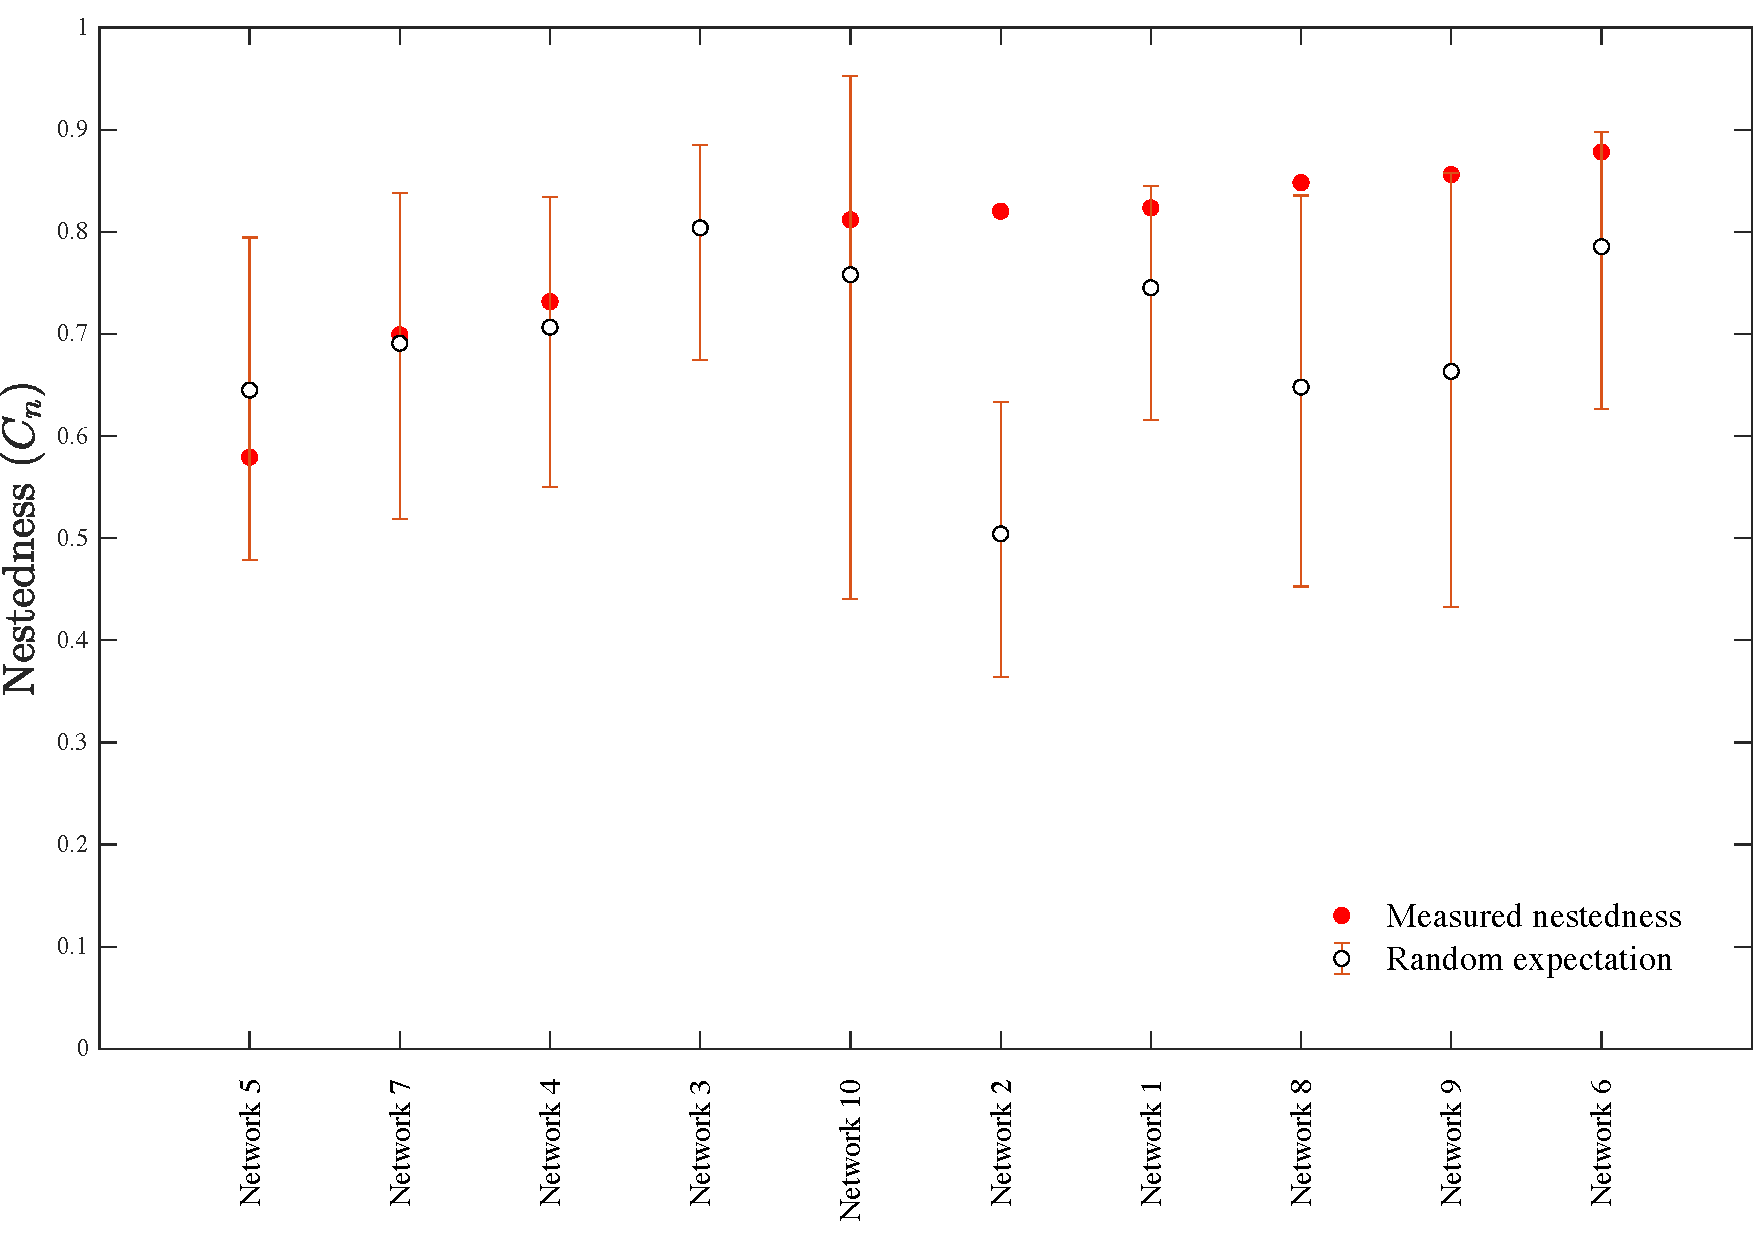
\includegraphics[width=1.4\linewidth,angle=0]{./Figures/1990_cc_nestedness_adjacency_matrices.pdf}
% \end{minipage}
% \caption{\label{fig:1990_cc_nestedness_modularity_adjacency_matrices} The top left panel shows the adjacency matrix of the largest connected component of the R\&D network in the year 1990 %(see Fig. \ref{fig:1990_cc_graph}) 
% where the modules identified are indicated with different colors. The top middle and top right panels zoom into the largest modules. The bottom left panel shows the adjacency matrices of each module (subnetwork) separately (showing only the first 10 modules with the highest modularity and size), where a (+) indicates that the matrix is statistically significantly nested at the 5\% level \citep{AlmeidaNeto2008}. The solid red line indicates the isocline (that is, a curve that divides the ones from the zeros of a perfectly nested matrix of the same size and connectivity). The bottom right panel shows the nestedness coefficients, $C_n$, of these 10 modules (sorted by $C_n$).% Figures have been created using the \texttt{BiMat} Matlab library (\url{https://bimat.github.io/}).
% }
% \end{figure}

% \begin{figure}
% \begin{center}
% Year: 2000
% \end{center}
% \begin{minipage}{\linewidth}
% \centering
% 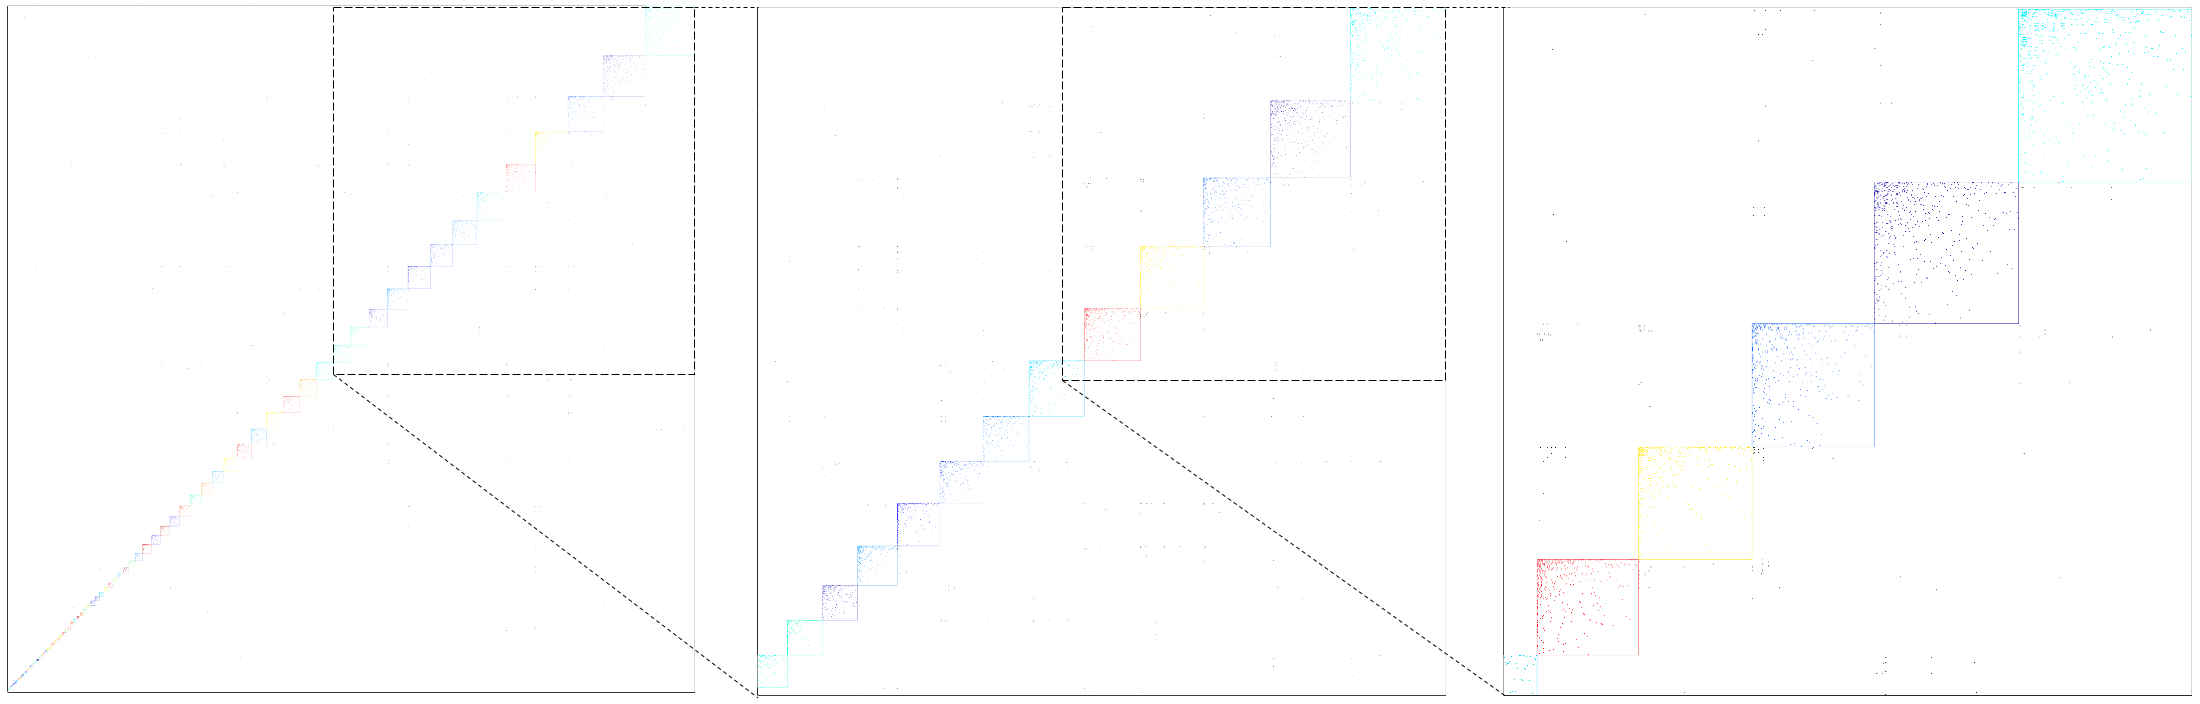
\includegraphics[width=\textwidth]{./Figures/2000_cc_modularity_adjacency_matrix_1_2_3.png}
% \end{minipage}
% \begin{minipage}{\linewidth}
% ${}$
% \end{minipage}
% \begin{minipage}{0.45\linewidth}
% \centering
% 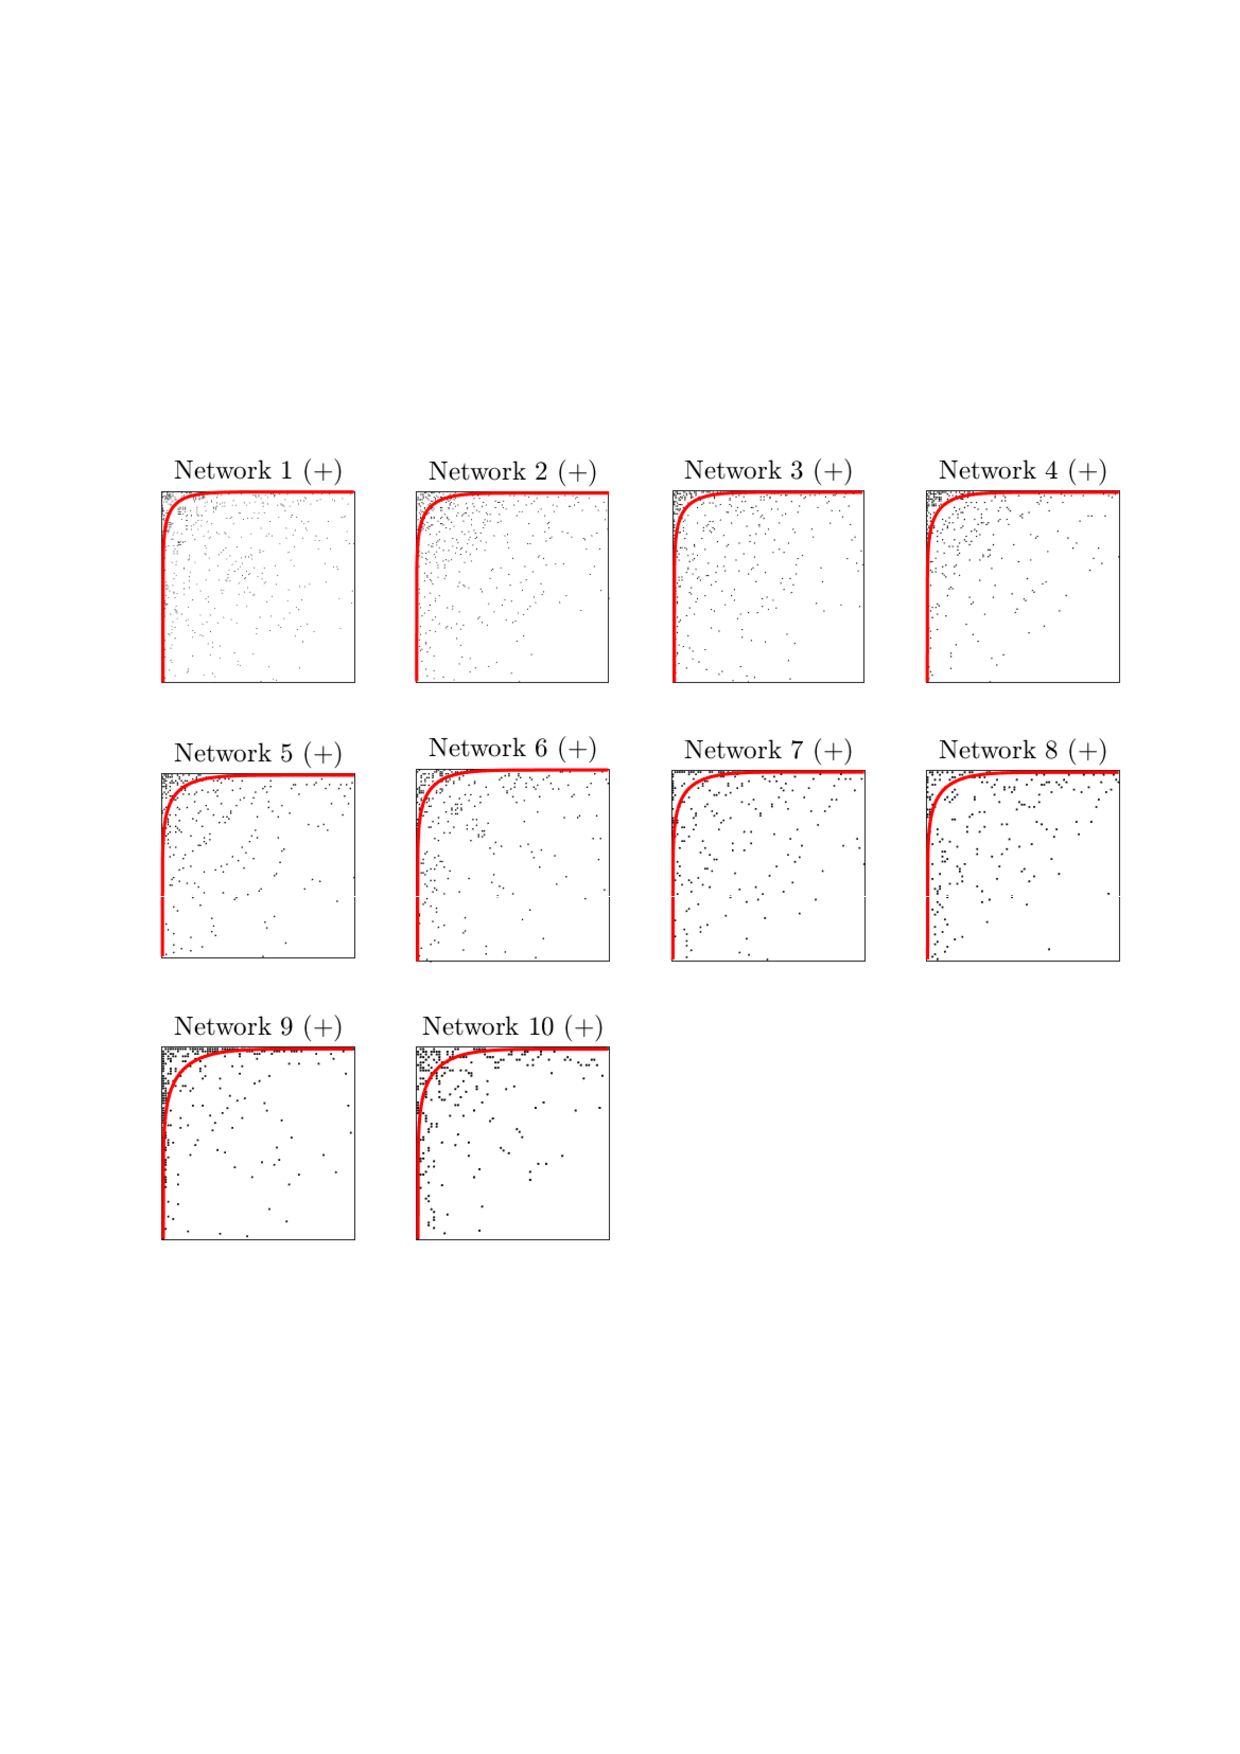
\includegraphics[width=\textwidth]{./Figures/2000_cc_adjacency_matrices.pdf}
% \end{minipage}
% \begin{minipage}{0.1\linewidth}
% \end{minipage}
% \begin{minipage}{0.3725\linewidth}
% \centering
% 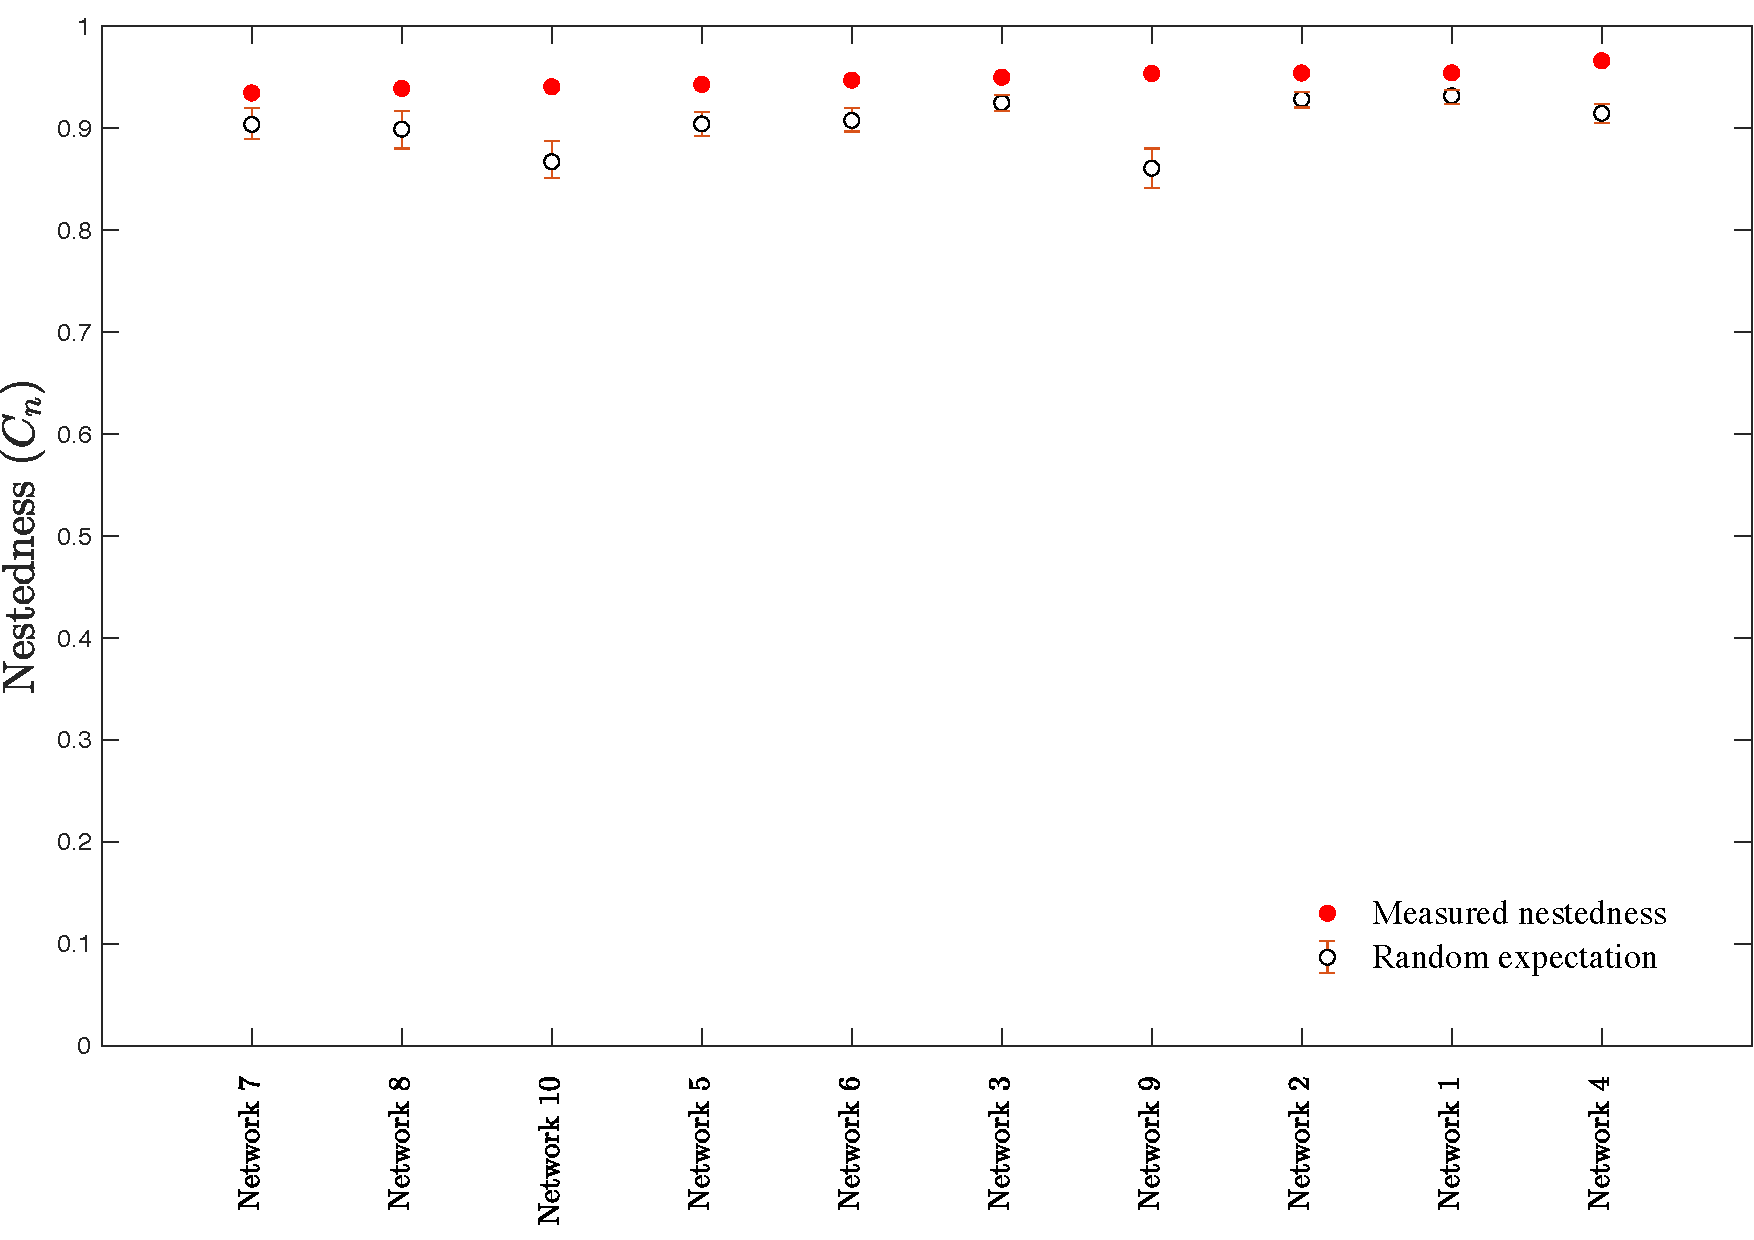
\includegraphics[width=1.4\linewidth,angle=0]{./Figures/2000_cc_nestedness_adjacency_matrices.pdf}
% \end{minipage}
% \caption{\label{fig:2000_cc_nestedness_modularity_adjacency_matrices} The top left panel shows the adjacency matrix of the largest connected component of the R\&D network in the year 2000 %(see Fig. \ref{fig:2000_cc_graph})
% where the modules identified are indicated with different colors. The top middle and top right panels zoom into the largest modules. The bottom left panel shows the adjacency matrices of each module (subnetwork) separately (showing only the first 10 modules with the highest modularity and size), where a (+) indicates that the matrix is statistically significantly nested at the 5\% level \citep{AlmeidaNeto2008}. The solid red line indicates the isocline (that is, a curve that divides the ones from the zeros of a perfectly nested matrix of the same size and connectivity). The bottom right panel shows the nestedness coefficients, $C_n$, of these 10 modules (sorted by $C_n$). % Figures have been created using the \texttt{BiMat} Matlab library (\url{https://bimat.github.io/}).
% }
% \end{figure}

% \begin{figure}
% \begin{center}
% Year: 2010
% \end{center}
% \begin{minipage}{\linewidth}
% \centering
% 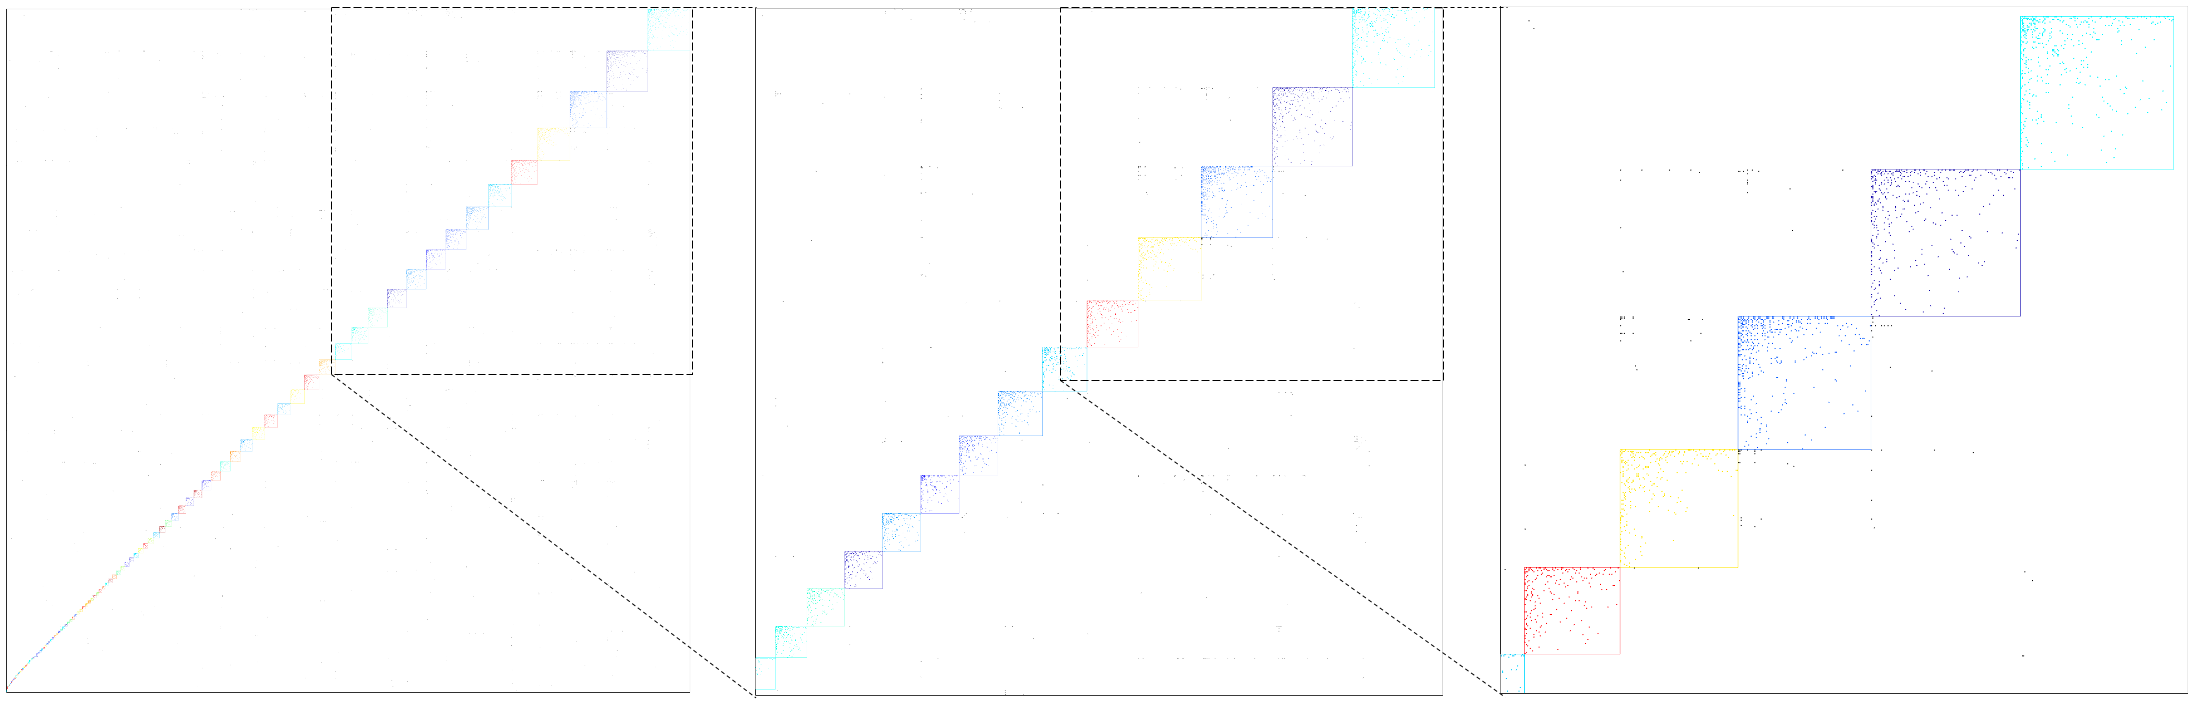
\includegraphics[width=\textwidth]{./Figures/2010_cc_modularity_adjacency_matrix_1_2_3.png}
% \end{minipage}
% \begin{minipage}{\linewidth}
% ${}$
% \end{minipage}
% \begin{minipage}{0.45\linewidth}
% \centering
% 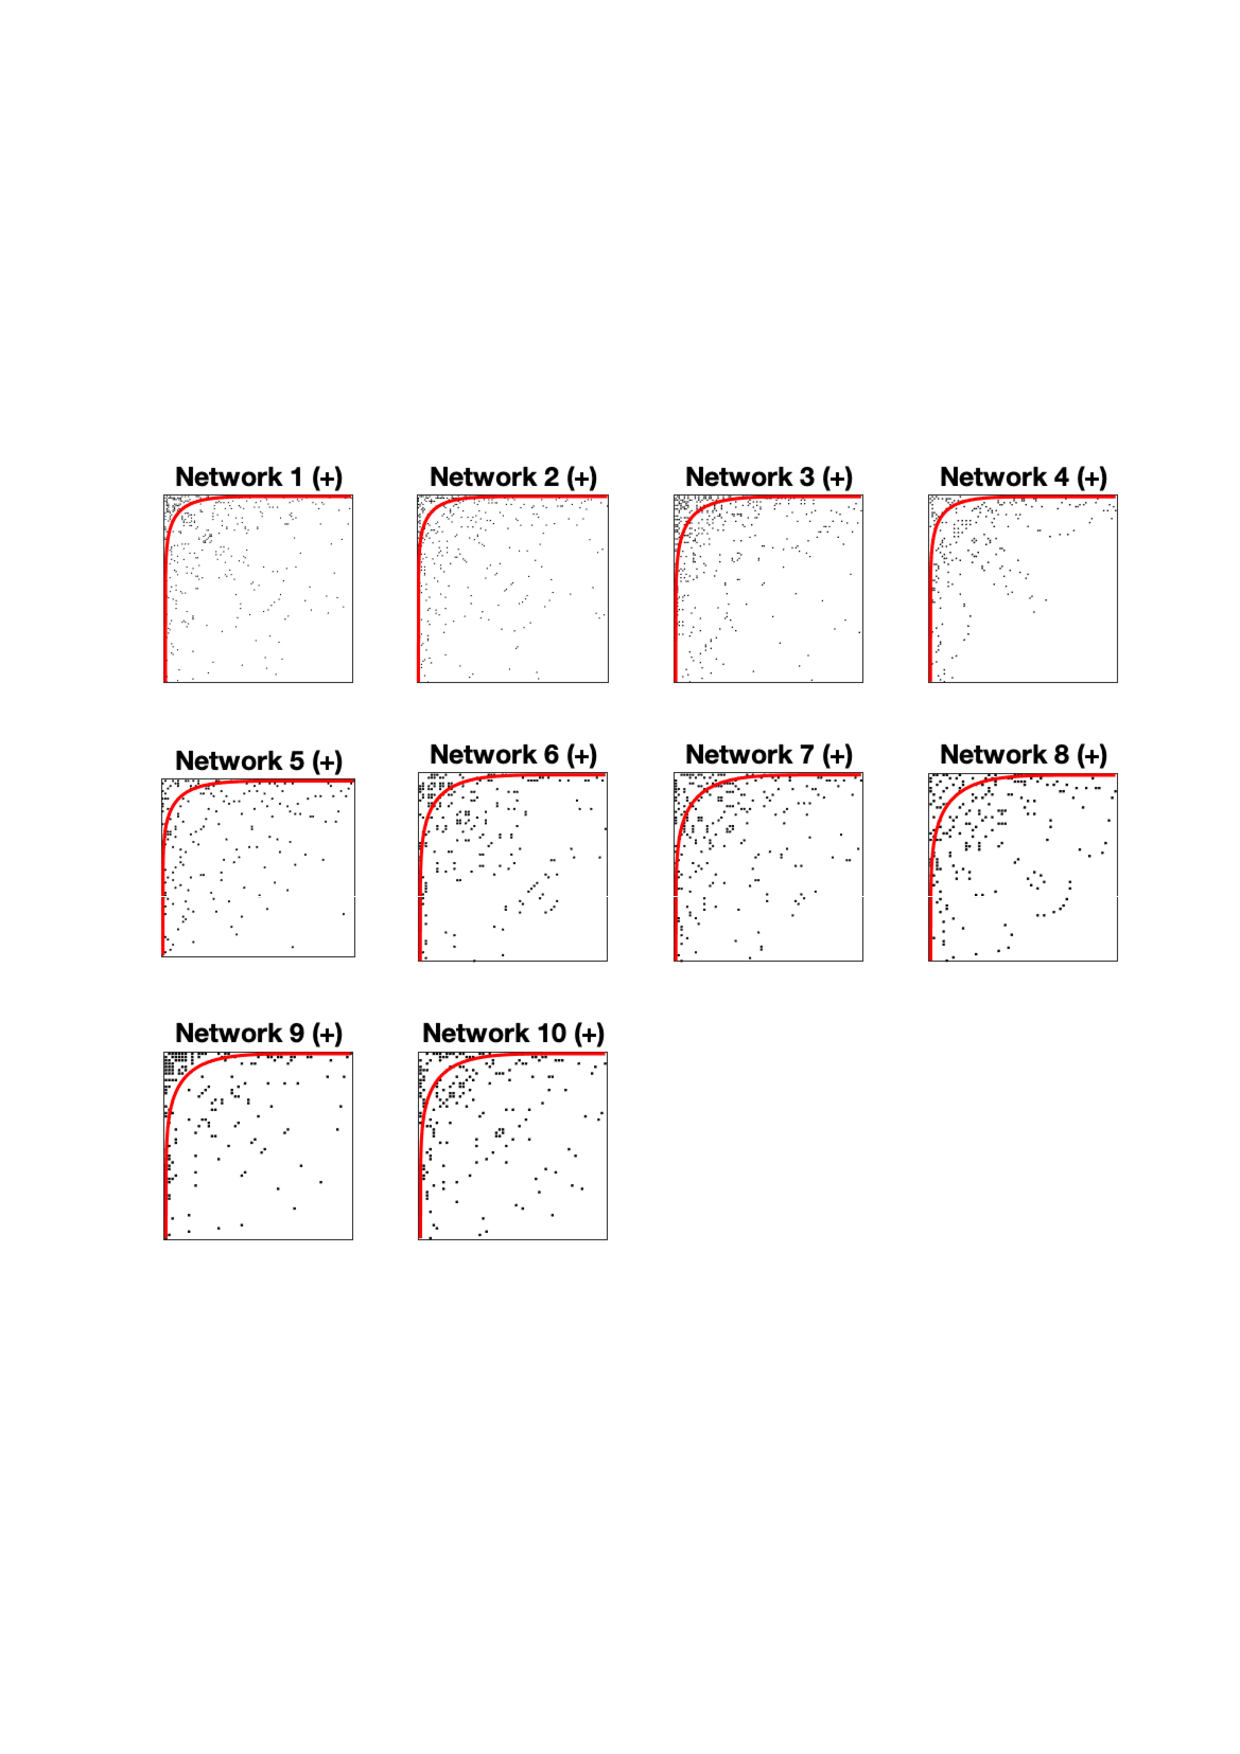
\includegraphics[width=\textwidth]{./Figures/2010_cc_adjacency_matrices.pdf}
% \end{minipage}
% \begin{minipage}{0.1\linewidth}
% \end{minipage}
% \begin{minipage}{0.3725\linewidth}
% \centering
% 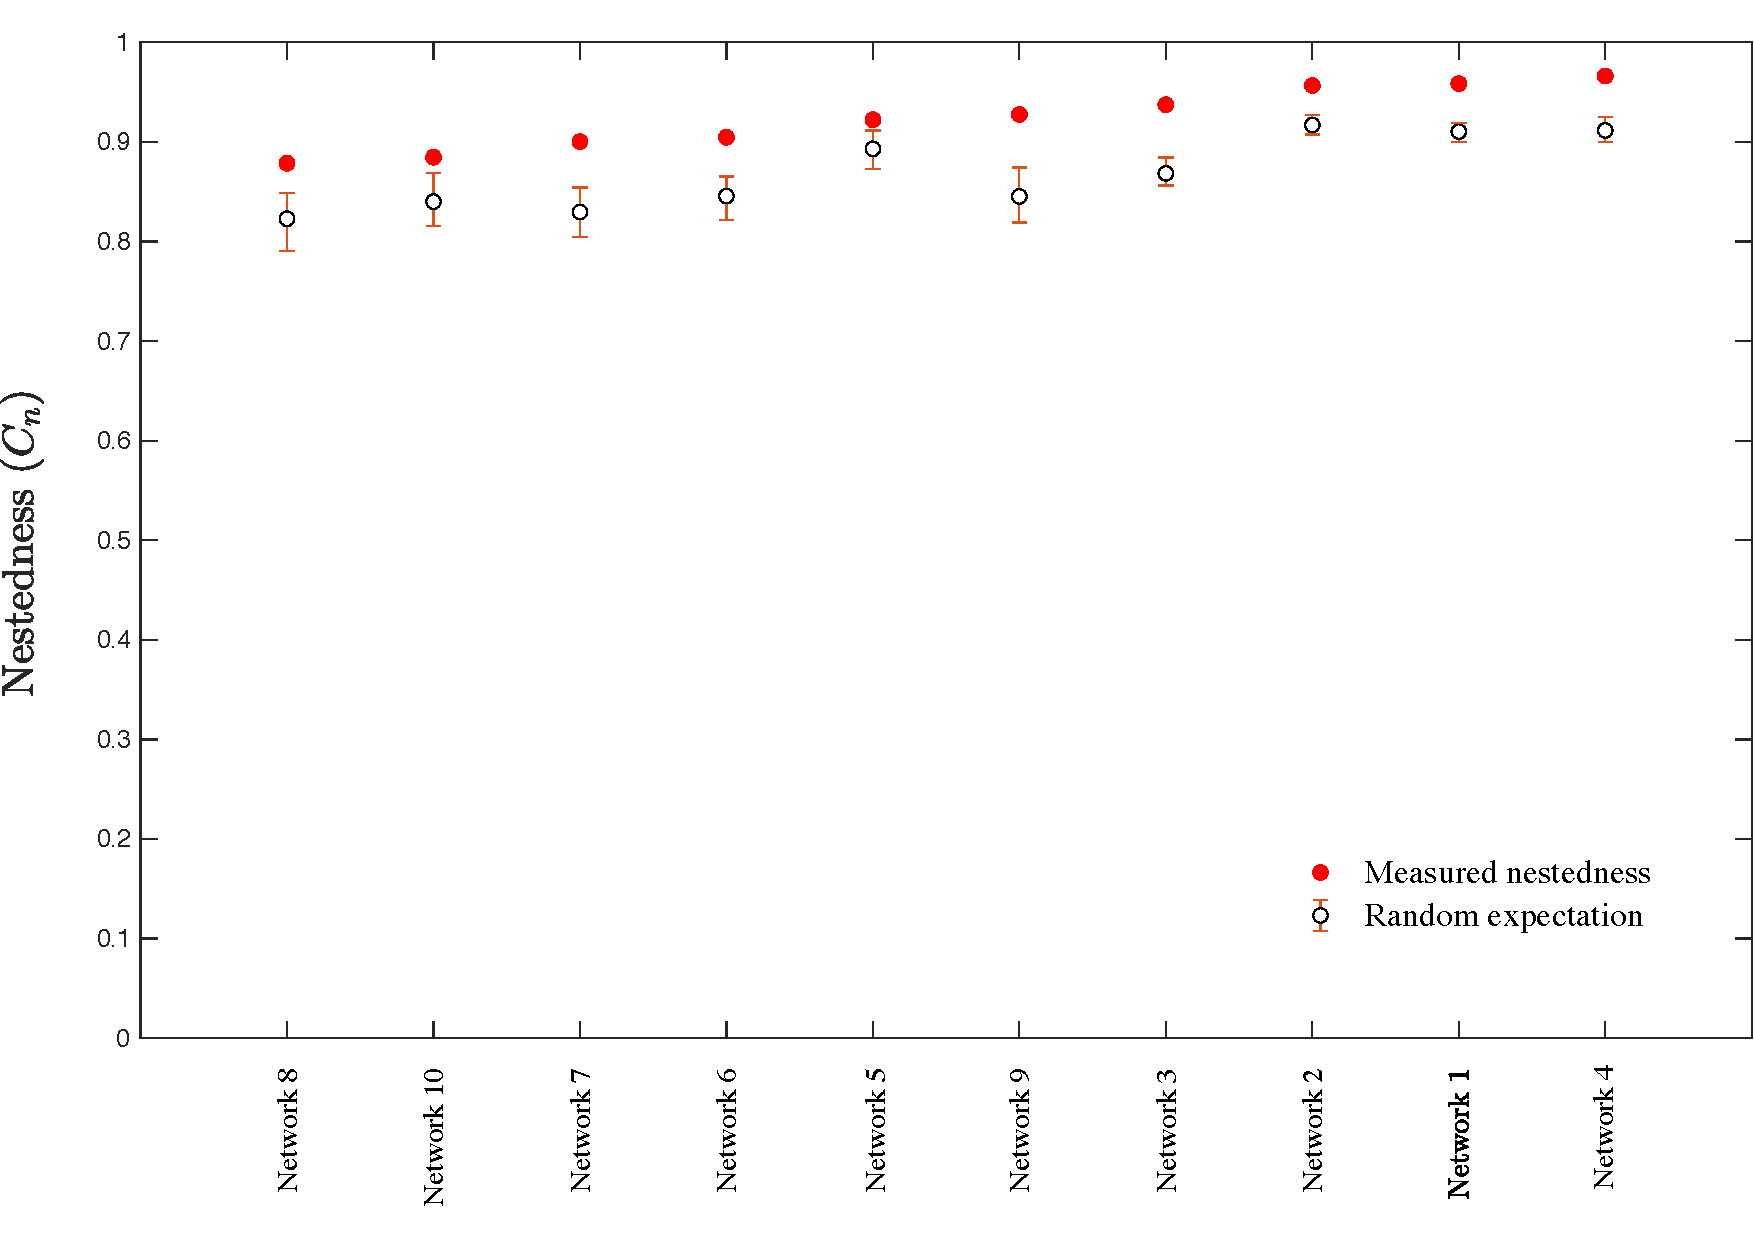
\includegraphics[width=1.4\linewidth,angle=0]{./Figures/2010_cc_nestedness_adjacency_matrices.pdf}
% \end{minipage}
% \caption{\label{fig:2010_cc_nestedness_modularity_adjacency_matrices} The top left panel shows the adjacency matrix of the largest connected component of the R\&D network in the year 2010  %(see Fig. \ref{fig:2010_cc_graph}) 
% where the modules identified are indicated with different colors. The top middle and top right panels zoom into the largest modules. The bottom left panel shows the adjacency matrices of each module (subnetwork) separately (showing only the first 10 modules with the highest modularity and size), where a (+) indicates that the matrix is statistically significantly nested at the 5\% level \citep{AlmeidaNeto2008}. The solid red line indicates the isocline (that is, a curve that divides the ones from the zeros of a perfectly nested matrix of the same size and connectivity). The bottom right panel shows the nestedness coefficients, $C_n$, of these 10 modules (sorted by $C_n$). %  Figures have been created using the \texttt{BiMat} Matlab library (\url{https://bimat.github.io/}).
% }
% \end{figure}

% \begin{figure}
% \begin{center}
% Year: 2020
% \end{center}
% \begin{minipage}{\linewidth}
% \centering
% 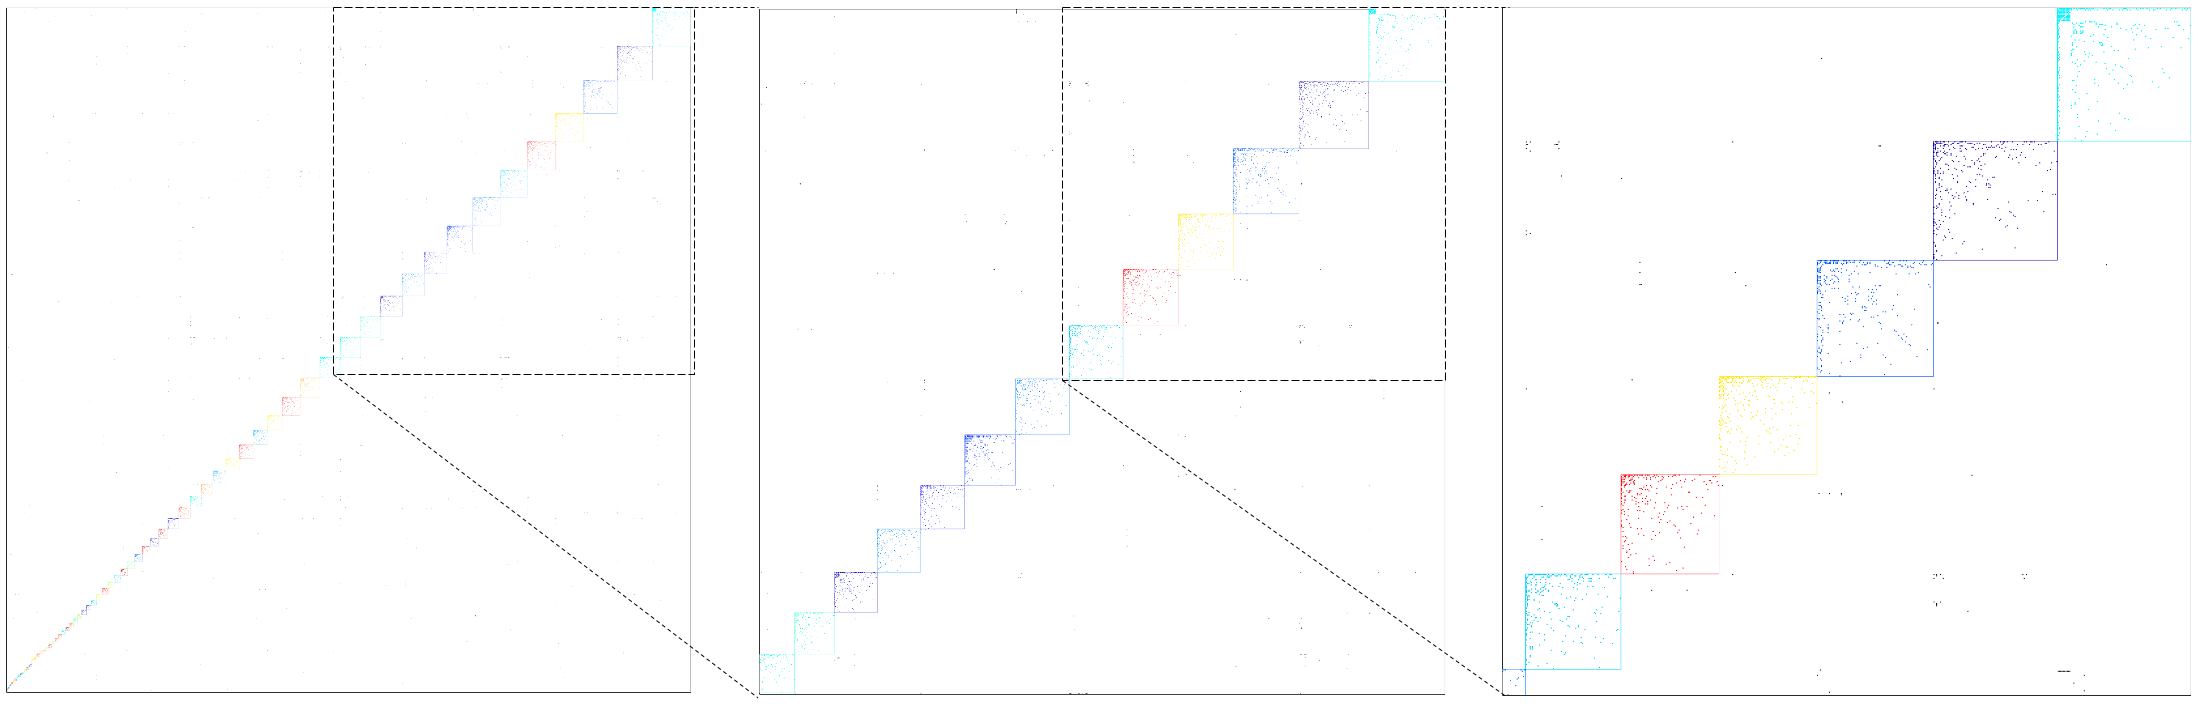
\includegraphics[width=\textwidth]{./Figures/2020_cc_modularity_adjacency_matrix_1_2_3.png}
% \end{minipage}
% \begin{minipage}{\linewidth}
% ${}$
% \end{minipage}
% \begin{minipage}{0.45\linewidth}
% \centering
% 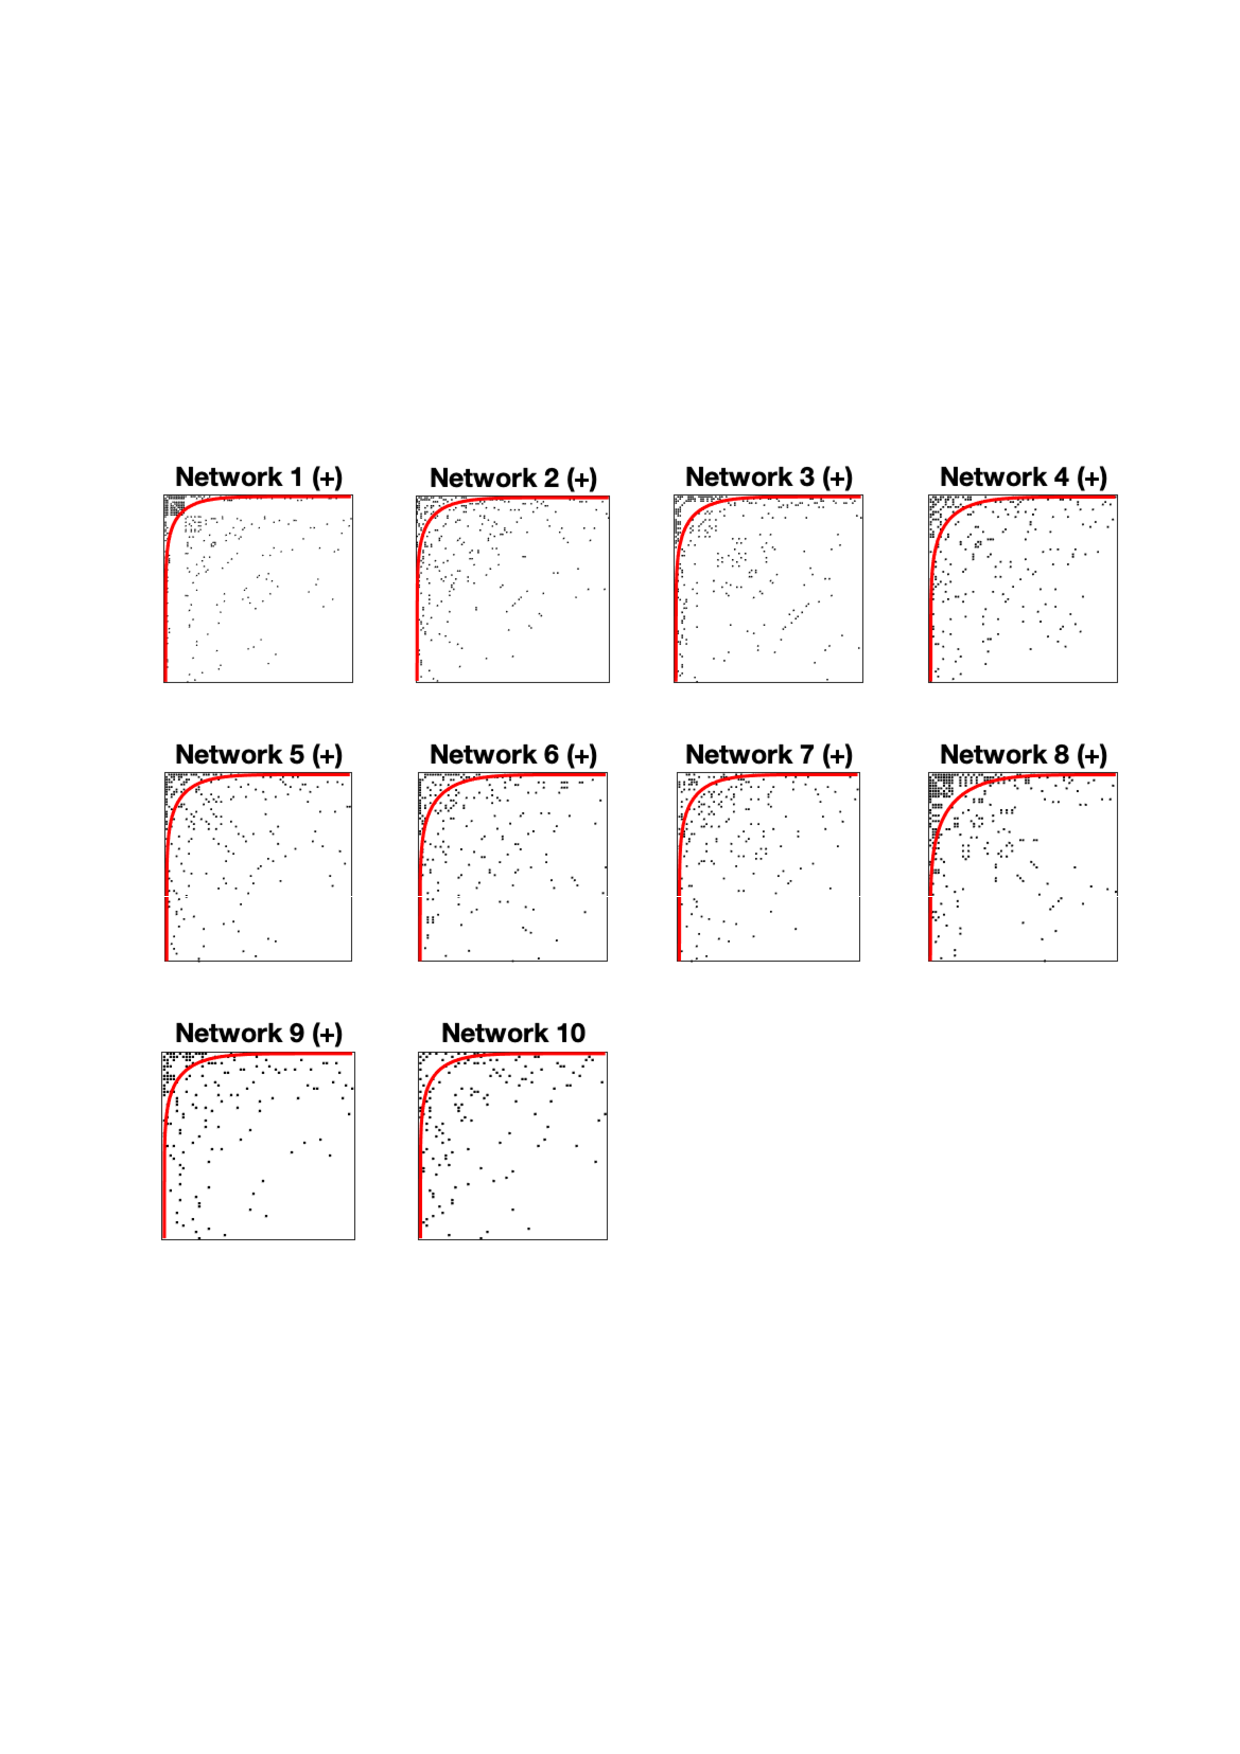
\includegraphics[width=\textwidth]{./Figures/2020_cc_adjacency_matrices.pdf}
% \end{minipage}
% \begin{minipage}{0.1\linewidth}
% \end{minipage}
% \begin{minipage}{0.3725\linewidth}
% \centering
% 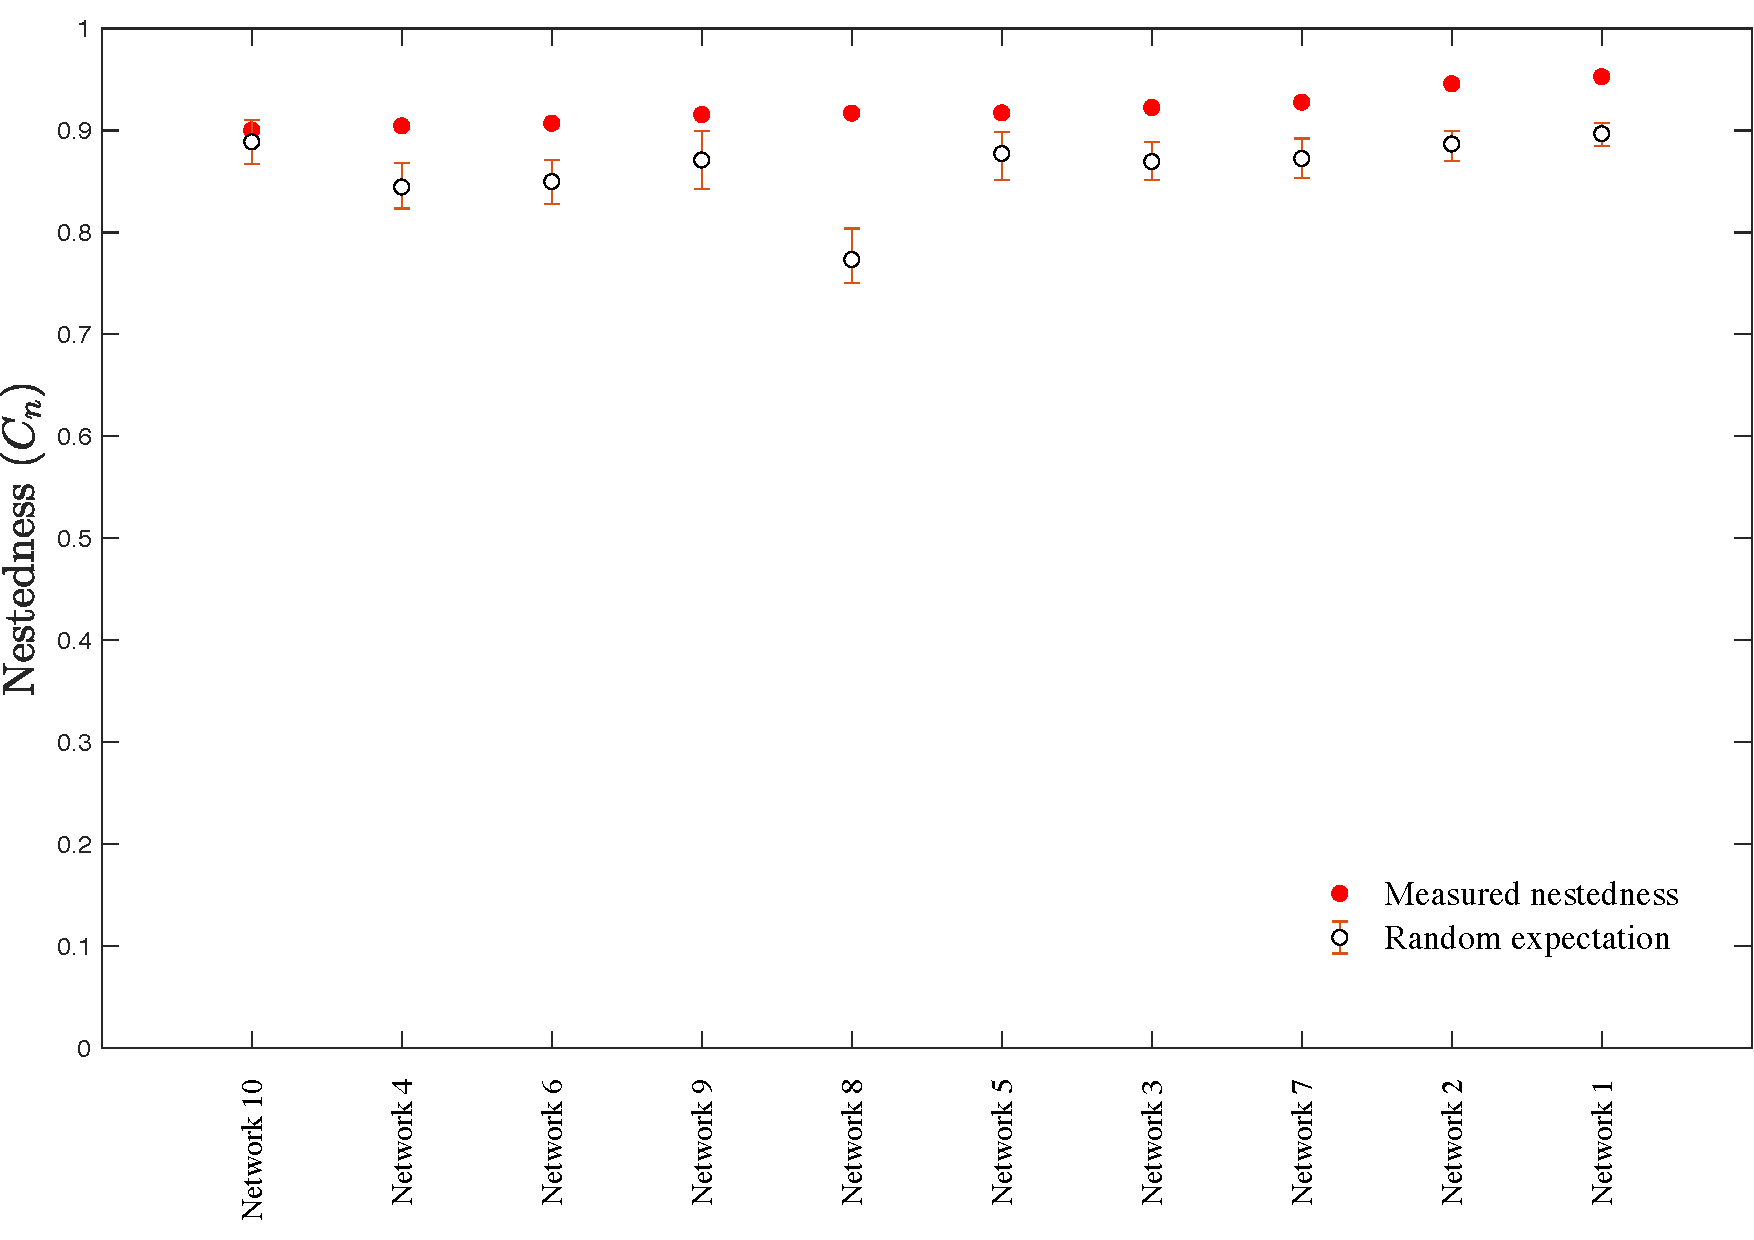
\includegraphics[width=1.4\linewidth,angle=0]{./Figures/2020_cc_nestedness_adjacency_matrices.pdf}
% \end{minipage}
% \caption{\label{fig:2020_cc_nestedness_modularity_adjacency_matrices} The top left panel shows the adjacency matrix of the largest connected component of the R\&D network in the year 2020 (see Fig. \ref{fig:2020_cc_graph}) where the modules identified are indicated with different colors. The top middle and top right panels zoom into the largest modules. The bottom left panel shows the adjacency matrices of each module (subnetwork) separately (showing only the first 10 modules with the highest modularity and size), where a (+) indicates that the matrix is statistically significantly nested at the 5\% level \citep{AlmeidaNeto2008}. The solid red line indicates the isocline (that is, a curve that divides the ones from the zeros of a perfectly nested matrix of the same size and connectivity). The bottom right panel shows the nestedness coefficients, $C_n$, of these 10 modules (sorted by $C_n$). % Figures have been created using the \texttt{BiMat} Matlab library (\url{https://bimat.github.io/}).
% }
% \end{figure}

%%%%%%%%%%%%%%%%%%%%%%%%%%%%%%%%%%%%%%%%%%%%%%%%%%%%%%%%%%
\subsection{\protect Orbis Company Information}
\label{sec:orbis}
%%%%%%%%%%%%%%%%%%%%%%%%%%%%%%%%%%%%%%%%%%%%%%%%%%%%%%%%%%
For company data, we use Bureau van Dijk's Orbis database. It contains firms' address and contact details, industry information (NACE codes), the number of employees; as well as financial information such as revenue, value added, assets, liabilities, and R\&D expenditure. We focus on companies for which all this information is available in the years up to 2021. We match the firm names detected in news articles to Orbis, after which we are left with 165,929 firms globally. The distribution of companies across sectors from the Orbis data can be seen in Figure \ref{fig:pie-2-dig-nace}.

\begin{figure}[tbp]
\centering
\centerline{ \scalebox{0.75}{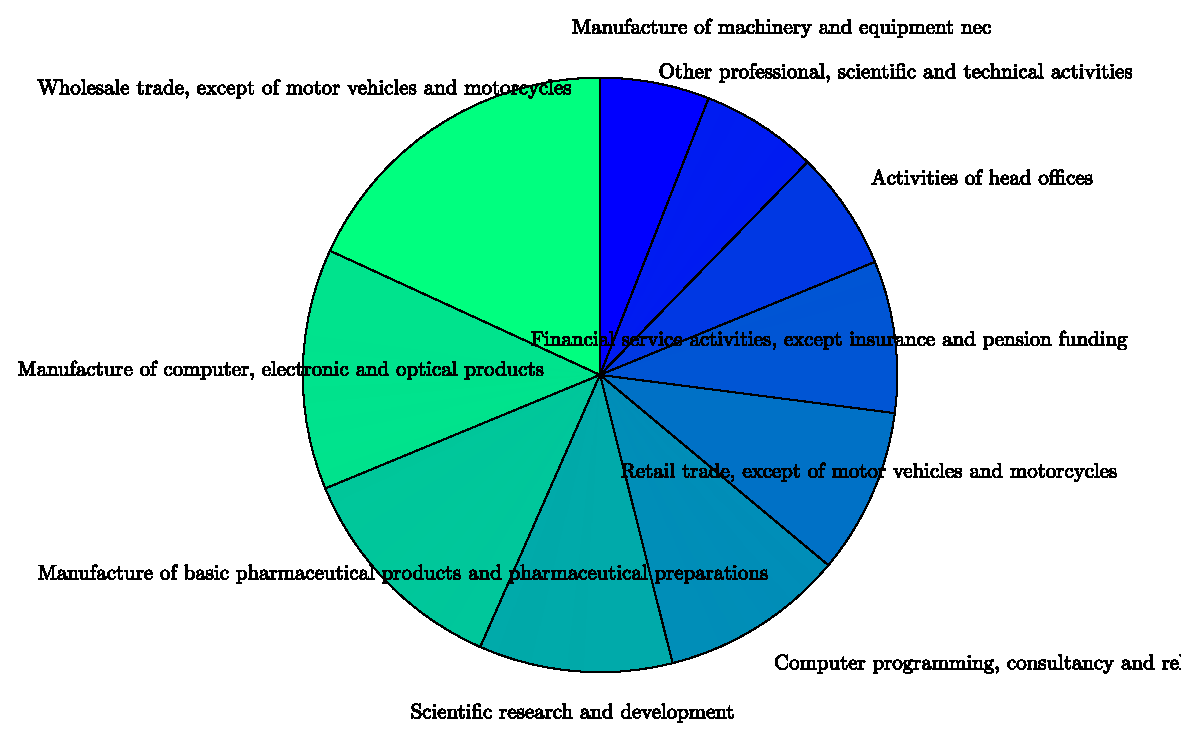
\includegraphics{./Figures/industries_2_dig_nace_distr.eps}}}
\caption{The shares of the ten largest sectors at the $2$-digit NACE Rev. 2 levels. See also Table \ref{tab:sic-rank-2-dig}, respectively. NACE refers to the current Statistical Classification of Economic Activities in the European Community (revision 2).}
\label{fig:pie-2-dig-nace}
\end{figure}

%%%%%%%%%%%%%%%%%%%%%%%%%%%%%%%%%%%%%%%%%%%%%%%%%%%%%%%%%%
\subsection{\protect Patent Data}
\label{sec:patents}
%%%%%%%%%%%%%%%%%%%%%%%%%%%%%%%%%%%%%%%%%%%%%%%%%%%%%%%%%%
The Worldwide Patent Statistical Database (PATSTAT) is provided by the European Patent Office (EPO). It covers patent applications to authorities in 90 countries. The data include: applicant and inventor names and addresses, filing date, titles, and abstracts of patent applications; technology classification and technically related patents, and bibliographical information such as number of citations and citation links. Our version of the database is from spring 2021.

Applicants in the database can be both natural and legal persons (while inventors may only be natural persons) and we focus on company applicants.\footnote{The exact query used was: psn\textunderscore sector in: 'COMPANY', 'COMPANY GOV NON-PROFIT', 'COMPANY GOV NON-PROFIT UNIVERSITY', 'COMPANY HOSPITAL', 'COMPANY UNIVERSITY', 'GOV NON-PROFIT', 'GOV NON-PROFIT HOSPITAL', 'GOV NON-PROFIT UNIVERSITY'.} We are left with around 3.6 million distinct companies, which filed 31.9 million patents, some 17.9 million of which were granted. We match company name and address to Orbis company name and address. We find that of the 122,246 firms in our sample, 18,709 have applied for at least one patent.

%%%%%%%%%%%%%%%%%%%%%%%%%%%%%%%%%%%%%%%%%%%%%%%%%%%%%%%%%%
\subsection{\protect Mergers and Acquisitions}
\label{sec:mna}
%%%%%%%%%%%%%%%%%%%%%%%%%%%%%%%%%%%%%%%%%%%%%%%%%%%%%%%%%%
To get the ownership history of the firms in our sample, we use the Thomson SDC Platinum M\&A dataset. We focus on completed mergers, acquisitions, and acquisitions of majority interest. There are 302,151 such transactions between the years 1971 and 2022. We match acquiror and target names, as well as the names of their ultimate parent (if applicable) to Orbis. See Figure \ref{fig:m_and_a_deals_thomson} for an illustration.

% \begin{figure}[tbp]
% \centering
% \centerline{ \scalebox{0.75}{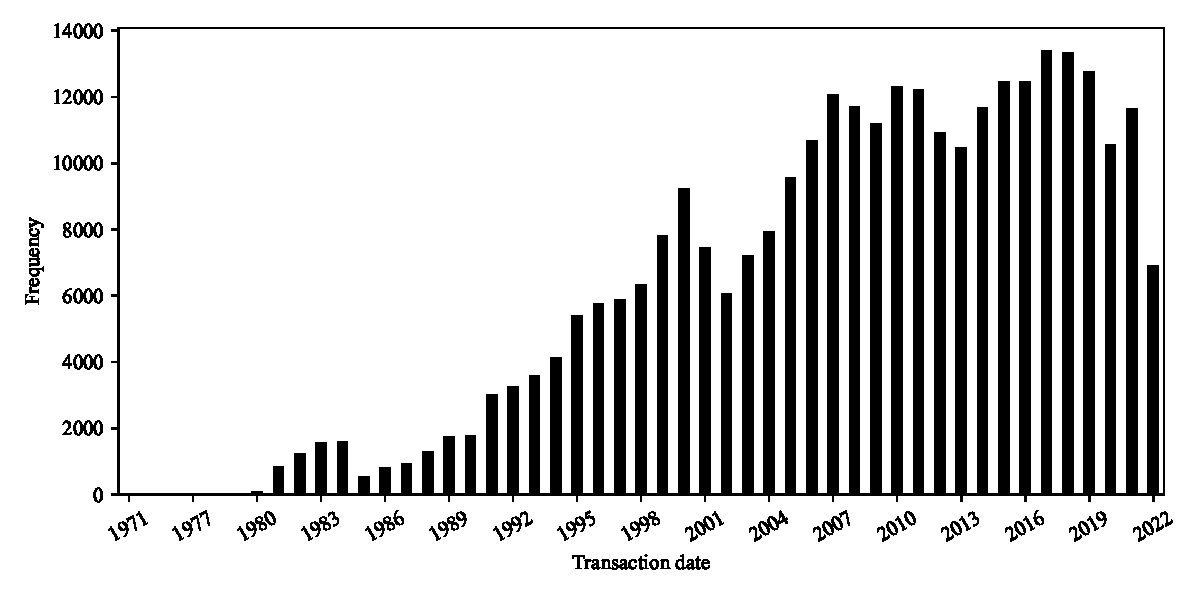
\includegraphics{./Figures/thomson_m_a_transactions_per_year.pdf}}}
% \caption{Completed mergers, acquisitions, and acquisitions of majority interest, per year in the Thomson SDC Platinum M\&A dataset.}
% \label{fig:m_and_a_deals_thomson}
% \end{figure}

\begin{figure}[tbp]
\centering
\centerline{ \scalebox{0.5}{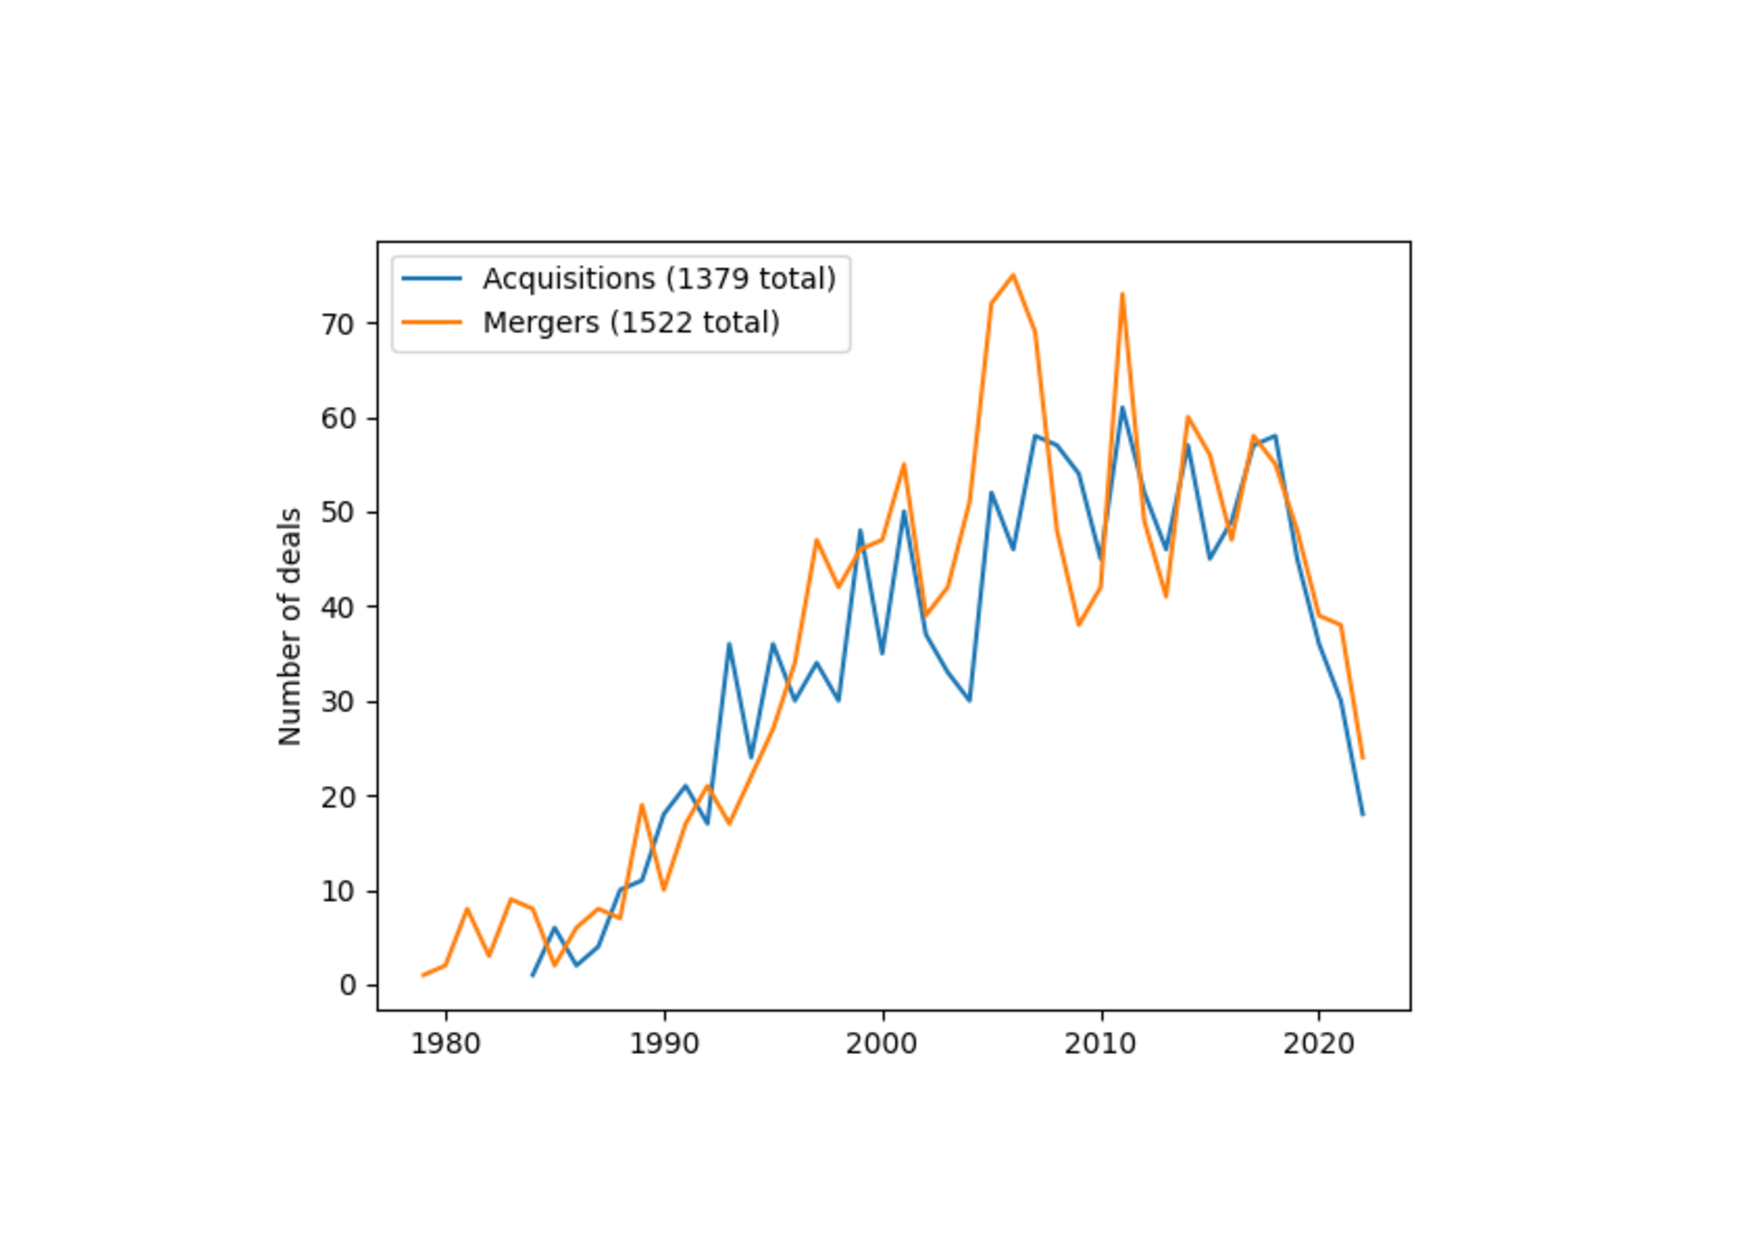
\includegraphics{./Figures/mna.pdf}}}
\caption{Completed mergers, acquisitions, and acquisitions of majority interest, per year in the Thomson SDC Platinum M\&A dataset of firms that participated also in R\&D collaborations.}
\label{fig:m_and_a_deals_thomson}
\end{figure}

\FloatBarrier

% %%%%%%%%%%%%%%%%%%%%%%%%%%%%%%%%%%%%%%%%%%%%%%%%%%%%%%%%%%
% \subsection{\protect Compustat Data, Interpolation and Imputation}
% \label{sec:compustat}
% %%%%%%%%%%%%%%%%%%%%%%%%%%%%%%%%%%%%%%%%%%%%%%%%%%%%%%%%%%
% Figures %\ref{fig:compustat-na-global}, \ref{fig:compustat-time-variation}, 
% \ref{fig:compustat-correlations} and \ref{fig:compustat-distr} show various descriptive statistics for the balance sheet data from the Compustat North America Fundamentals Annual and Compustat Global databases merged with the firms participating in R\&D collaborations. All variables reported in local currencies in the Compustat Global database have been translated into US dollars. Dollar values have then been deflated using the Consumer Price Index (CPI) from the US Bureau of Labor Statistics (\url{https://www.bls.gov/cpi/}) with 1983 as the base year with an index of 100. Output has been computed using the Producer Price Index (PPI) of the US Bureau of Labor Statistics (\url{https://www.bls.gov/ppi/}) matched to the year and NAICS code reported in the Compsutat sales item. Value added has been computed from Compustat data following the procedure in \citet{liu2018upward} and \citet{imrohorouglu2014firm}.\footnote{Value added can be computed from Compustat data using the following steps: $VALUE\_ADDED = SALES - MATERIALS, MATERIALS = TOTAL\_EXPENSES - LABOR\_EXPENSES$, where $TOTAL\_EXPENSES = SALES - OIBDP$, $LABOR\_EXPENSES = EMP * WAGE$. $WAGE$ is the average wage from the US Social Security Administration, and $OIBDP$ is the Compustat item ``Operating Income Before Depreciation and Amortization''. Putting the above together yields $VALUE\_ADDED = SALES - MATERIALS = SALES - (TOTAL\_EXPENSES - LABOR\_EXPENSES) = SALES - ((SALES - OIBDP) - LABOR\_EXPENSES) = SALES - ((SALES - OIBDP) - EMP * WAGE) = OIBDP + EMP * WAGE$.} The linear interpolation uses multiple observations of the same firm over different years, when there are gaps between the observations across years for the same firm (using Stata's ``ipolate'' function). The imputation method is based on the predictive mean
% matching imputation method (using Stata's ``mi impute pmm'' function) using industry, location and covariates (sales, R\&D, employment, output, etc.) as input \citep{rubin1986statistical}.

% \begin{figure}[tbp]
% \begin{minipage}{0.32\linewidth}
% \centering
% 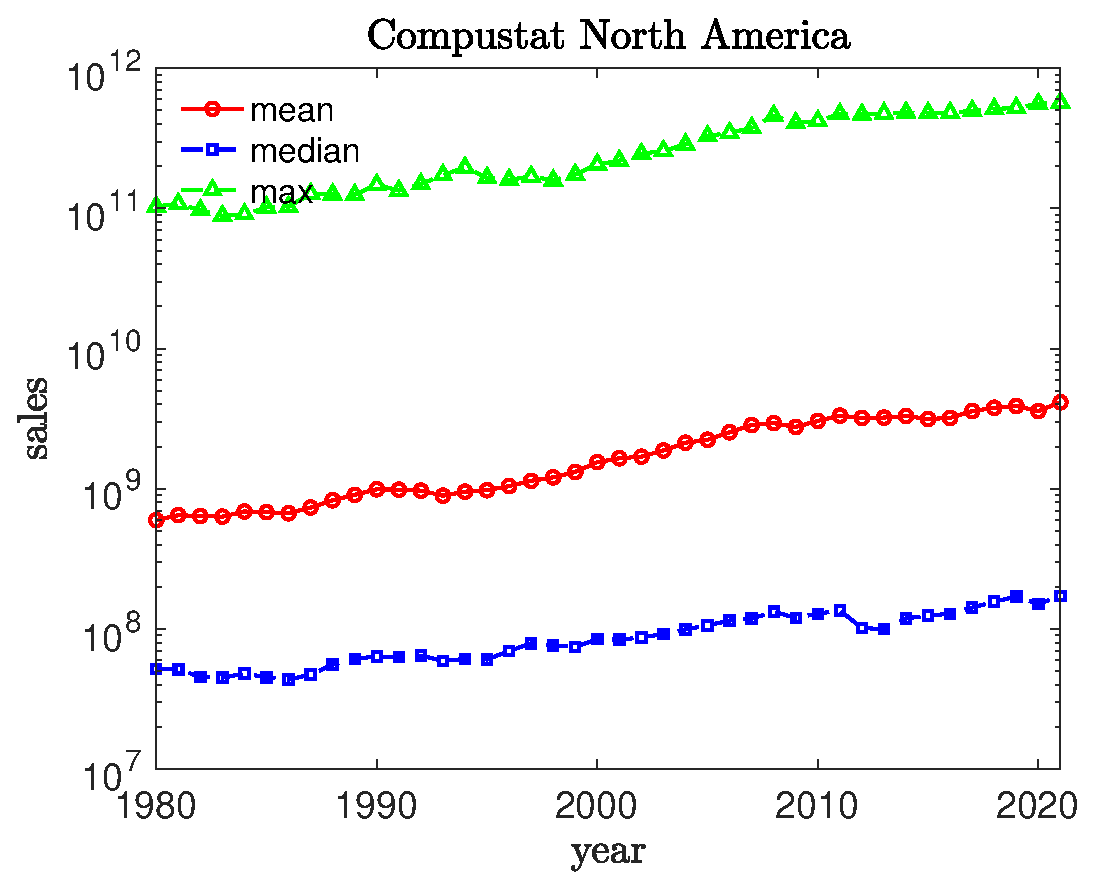
\includegraphics[width=5.4cm,angle=0]{./Figures/compustat_1980_2021_sales_years_comp_na.eps}
% \end{minipage}
% \begin{minipage}{0.32\linewidth}
% \centering
% 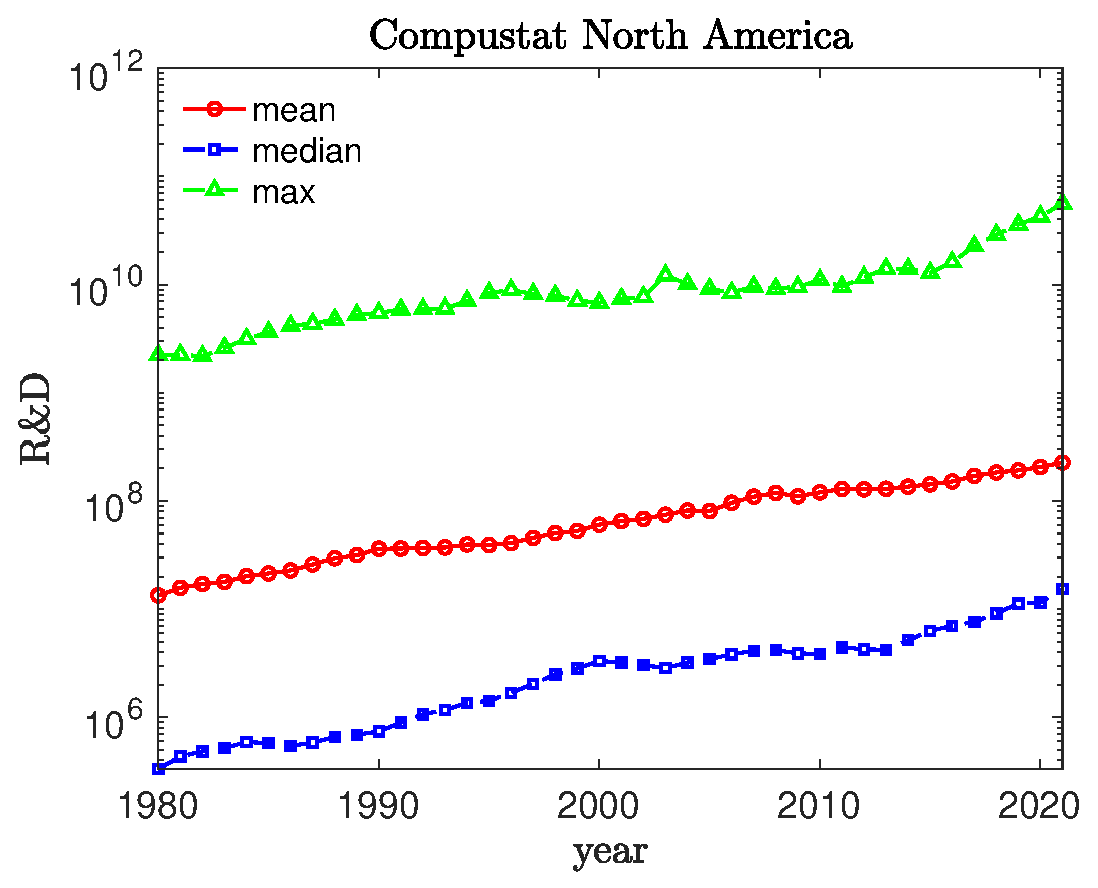
\includegraphics[width=5.4cm,angle=0]{./Figures/compustat_1980_2021_rnd_years_comp_na.eps}
% \end{minipage}
% \begin{minipage}{0.33\linewidth}
% \centering
% 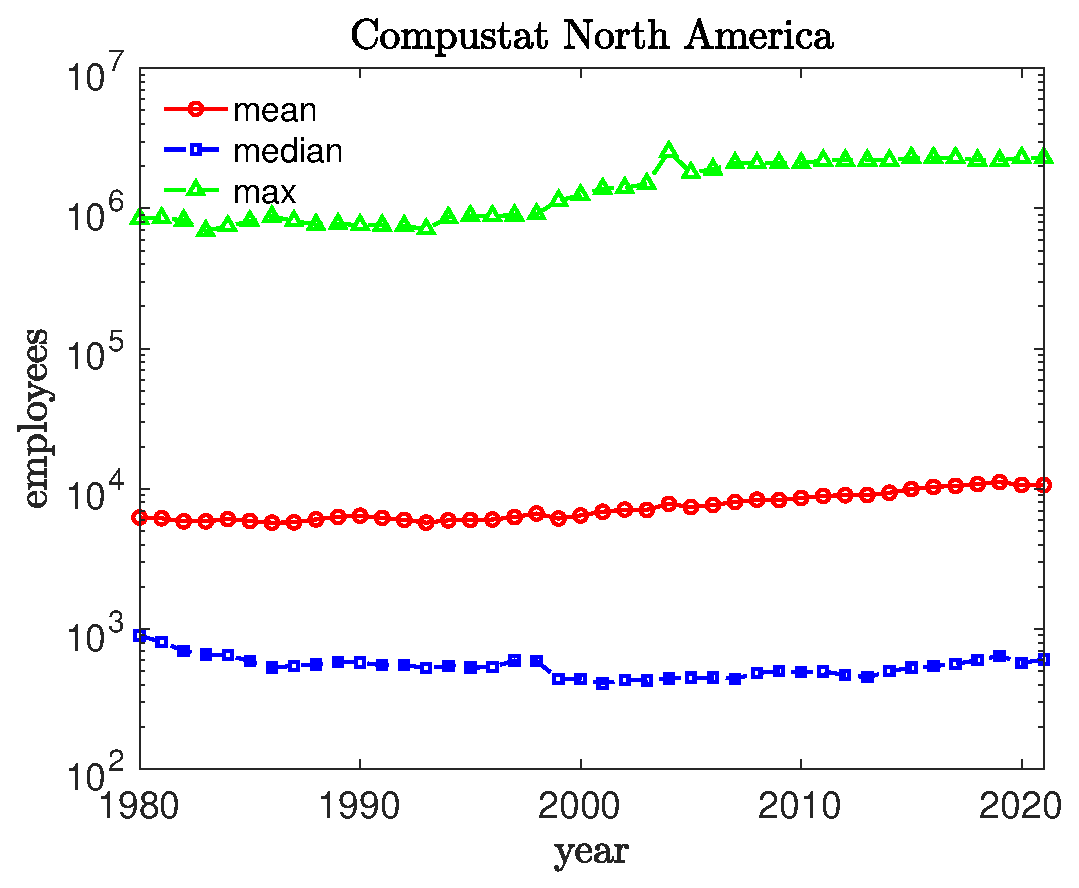
\includegraphics[width=5.4cm,angle=0]{./Figures/compustat_1980_2021_empl_years_comp_na.eps}
% \end{minipage}
% %
% \begin{minipage}{0.33\linewidth}
% \centering
% 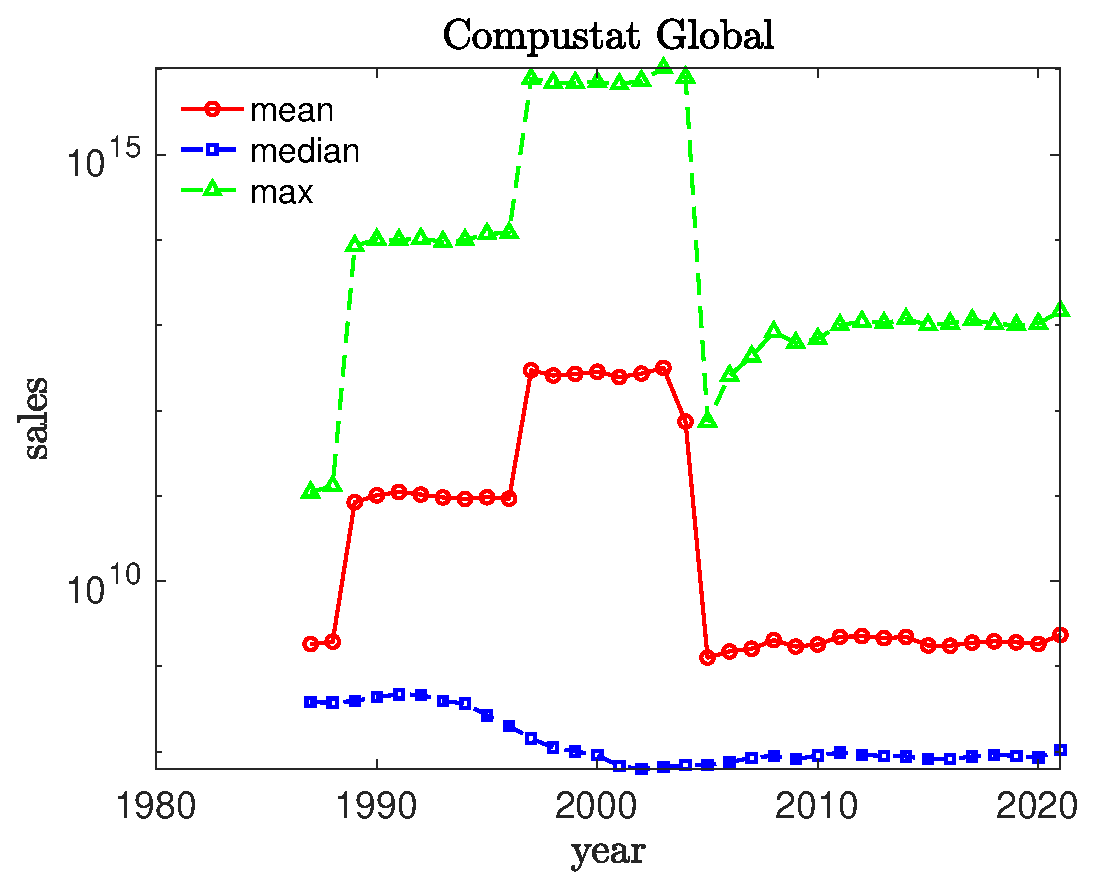
\includegraphics[width=5.4cm,angle=0]{./Figures/compustat_1980_2021_sales_years_comp_global.eps}
% \end{minipage}
% \begin{minipage}{0.33\linewidth}
% \centering
% 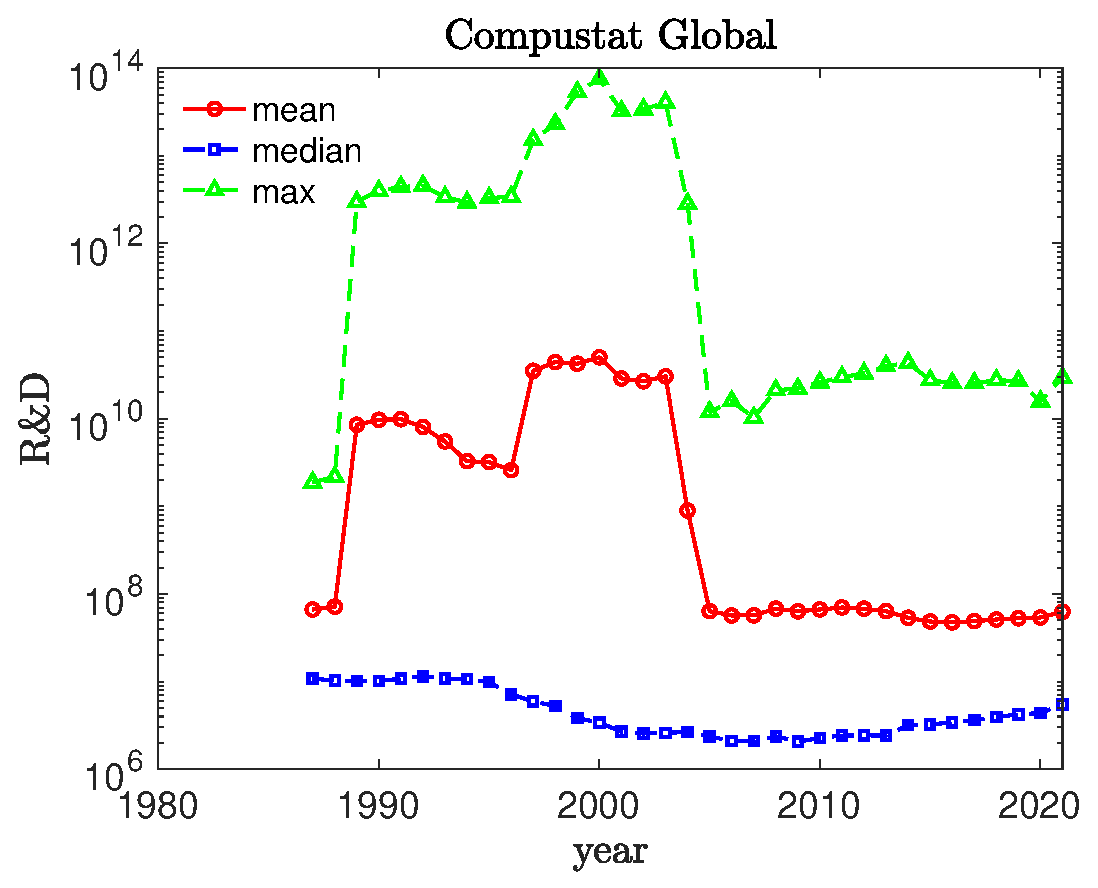
\includegraphics[width=5.4cm,angle=0]{./Figures/compustat_1980_2021_rnd_years_comp_global.eps}
% \end{minipage}
% \begin{minipage}{0.33\linewidth}
% \centering
% 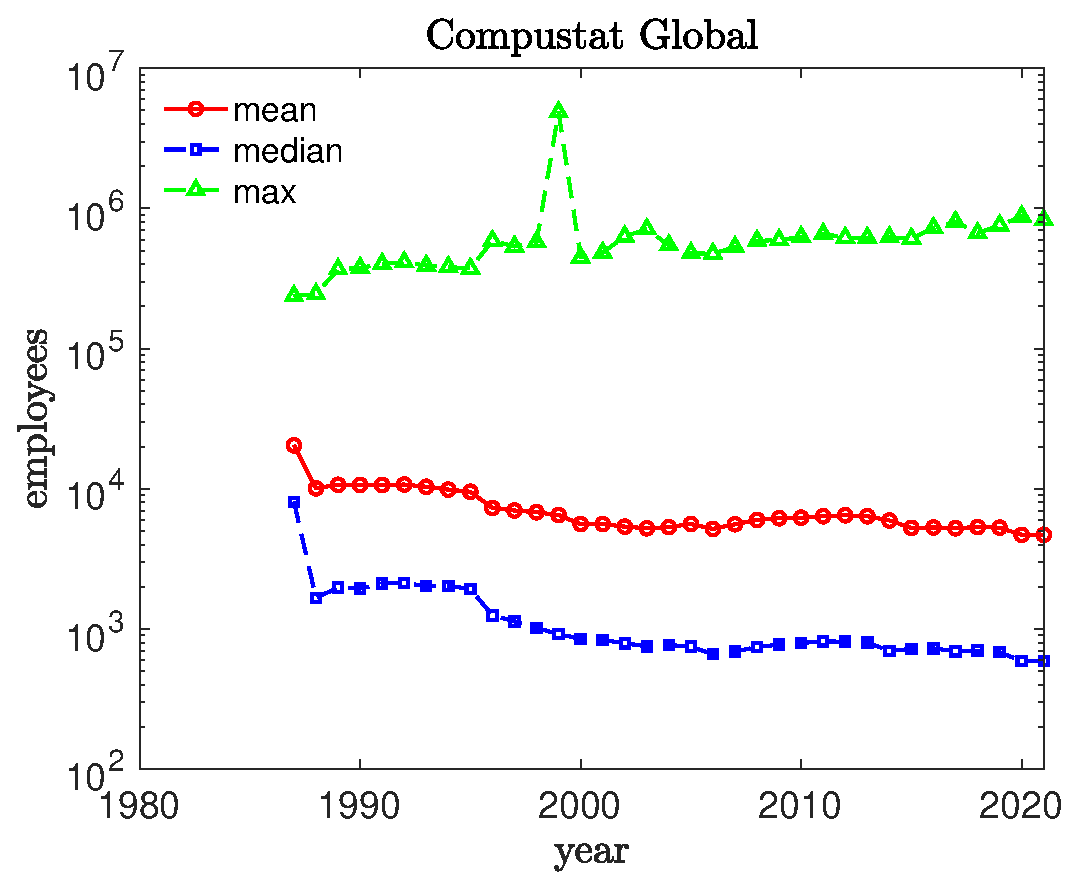
\includegraphics[width=5.4cm,angle=0]{./Figures/compustat_1980_2021_empl_years_comp_global.eps}
% \end{minipage}
% \caption{The top panels show the time variation of average, mean and maximum sales (left panel), R\&D expenditures (middle panel) and employment (right panel) of the years 1980 to 2021 for the Compustat North America Fundamentals Annual database. The bottom panels show the same figures for the Compustat Global database.}
% \label{fig:compustat-na-global}
% \end{figure}

% \begin{landscape}
% \begin{figure}[tbp]
% \begin{minipage}{0.24\linewidth}
% \centering
% {\small Comp. NA \& Global \phantom{(interpol. \& imputed)}}
% 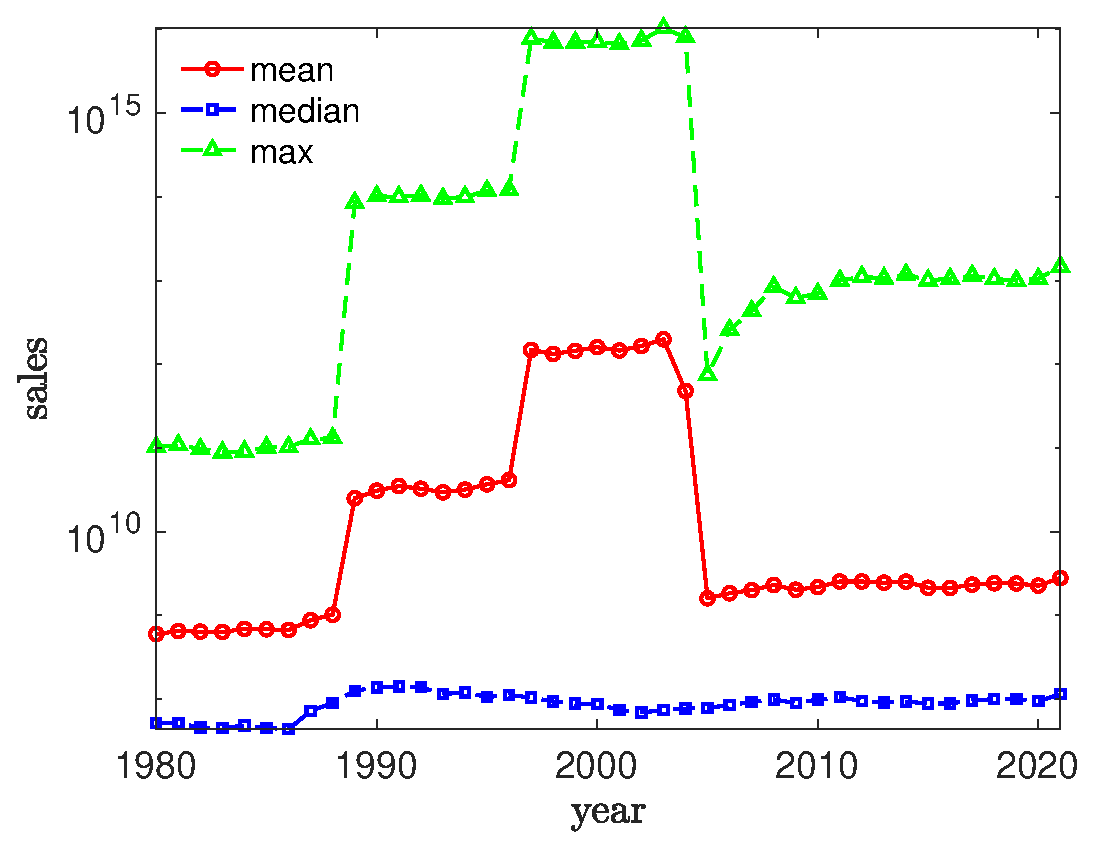
\includegraphics[width=5.25cm,angle=0]{./Figures/compustat_1980_2021_sales_years.eps}
% \end{minipage}
% \begin{minipage}{0.24\linewidth}
% \centering
% {\small Comp. NA \& Global (interpol. \& imputed)}
% 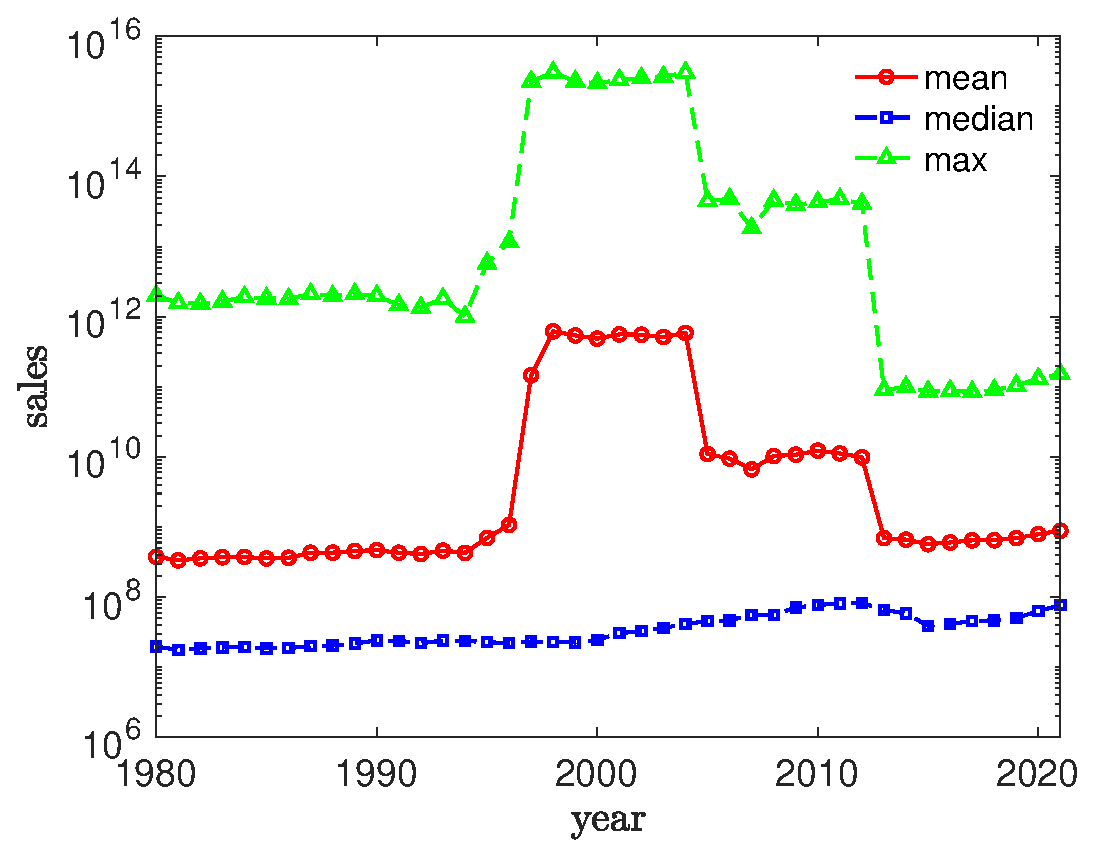
\includegraphics[width=5.25cm,angle=0]{./Figures/compustat_1980_2021_sales_years_lin_interpol_imputed.eps}
% \end{minipage}
% \begin{minipage}{0.245\linewidth}
% \centering
% {\small R\&D collab. firms only \phantom{(interpol. \& imputed)}}
% 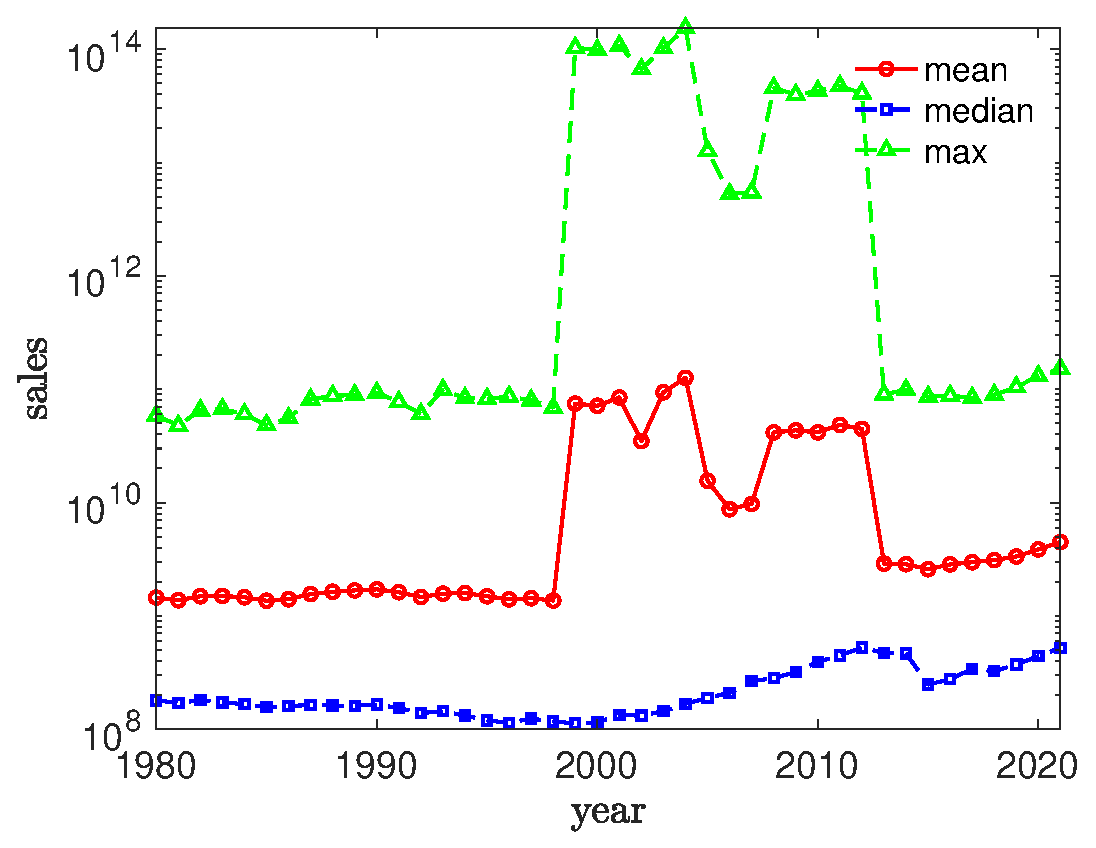
\includegraphics[width=5.25cm,angle=0]{./Figures/compustat_1980_2021_sales_years_rnd_coll_only.eps}
% \end{minipage}
% \begin{minipage}{0.25\linewidth}
% \centering
% {\small R\&D collab. firms only (interpol. \& imputed)}
% 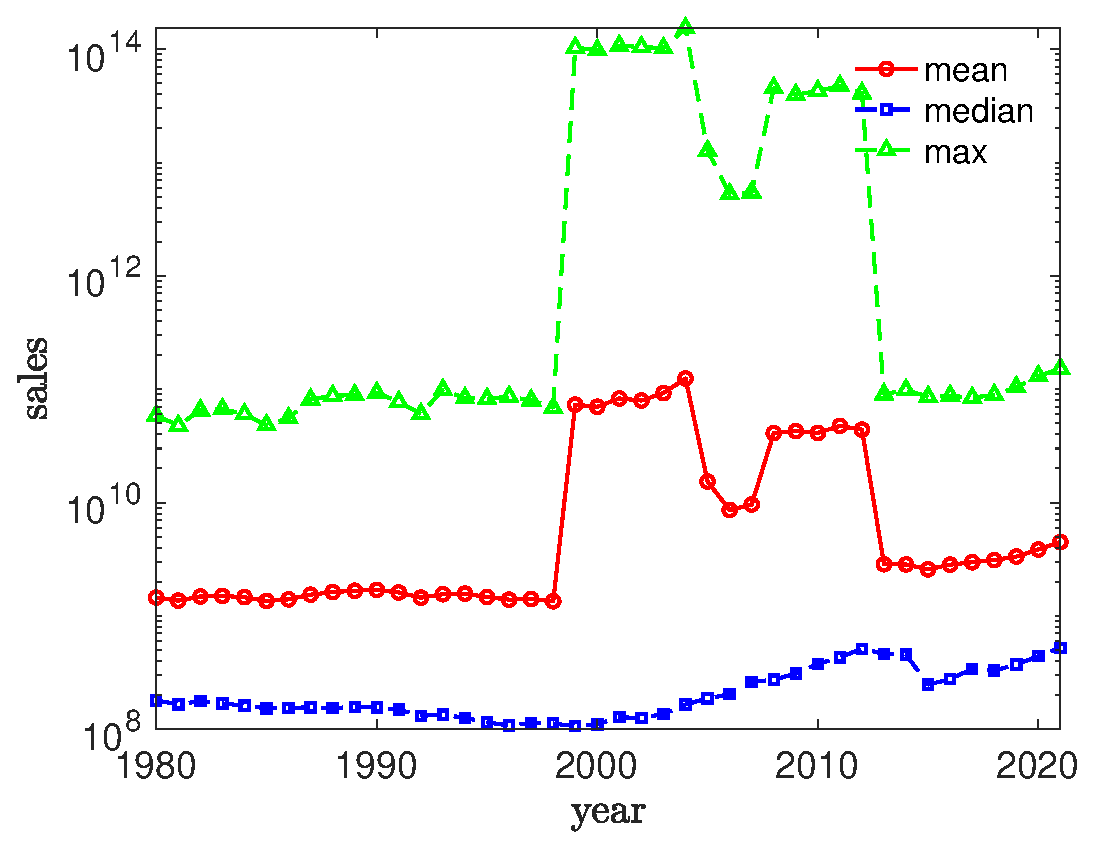
\includegraphics[width=5.25cm,angle=0]{./Figures/compustat_1980_2021_sales_years_lin_interpol_imputed_rnd_coll_only.eps}
% \end{minipage}
% %
% %
% \begin{minipage}{0.24\linewidth}
% \centering
% 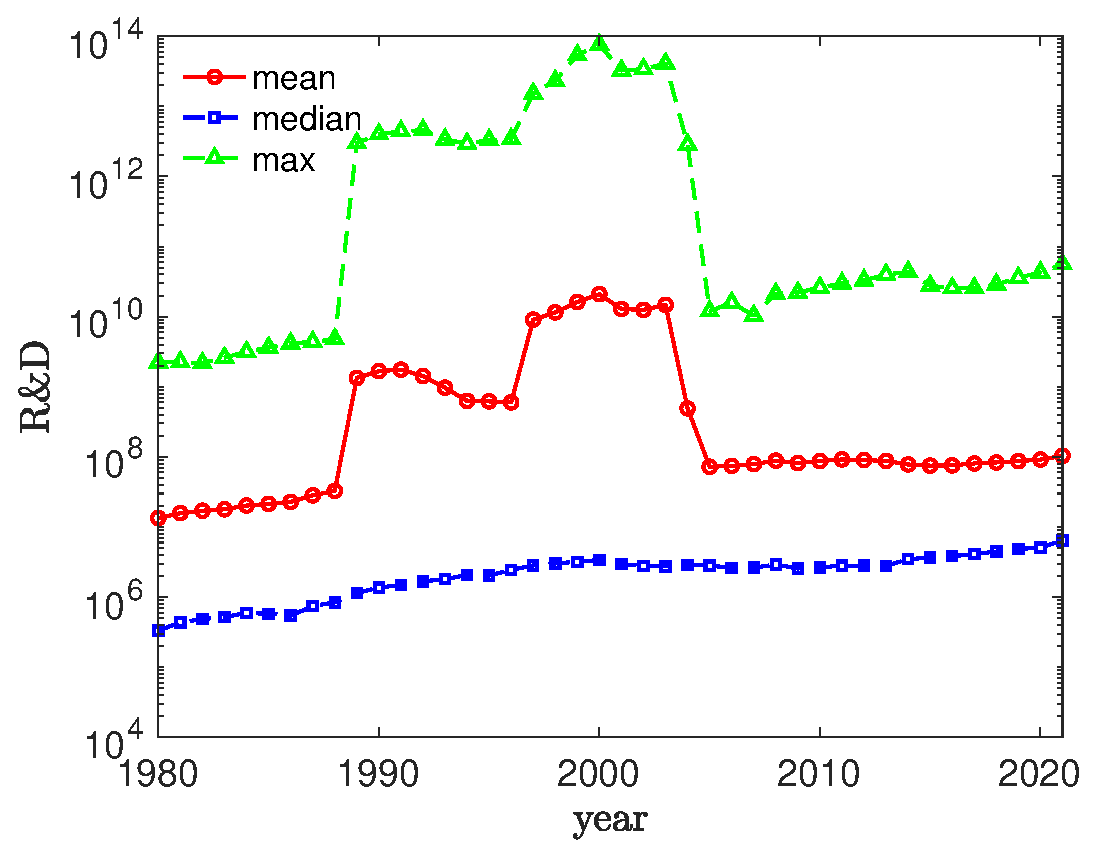
\includegraphics[width=5.25cm,angle=0]{./Figures/compustat_1980_2021_rnd_years.eps}
% \end{minipage}
% \begin{minipage}{0.24\linewidth}
% 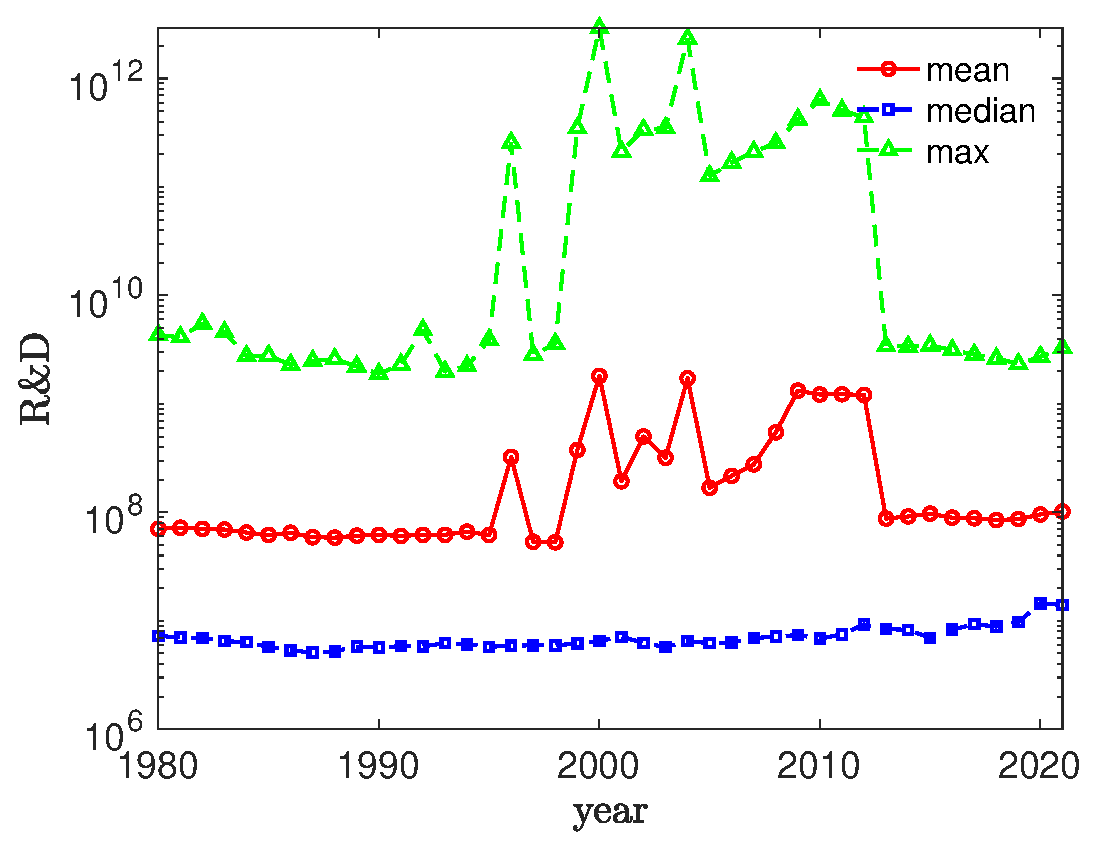
\includegraphics[width=5.25cm,angle=0]{./Figures/compustat_1980_2021_rnd_years_lin_interpol_imputed_rnd_coll_only.eps}
% \end{minipage}
% \begin{minipage}{0.25\linewidth}
% 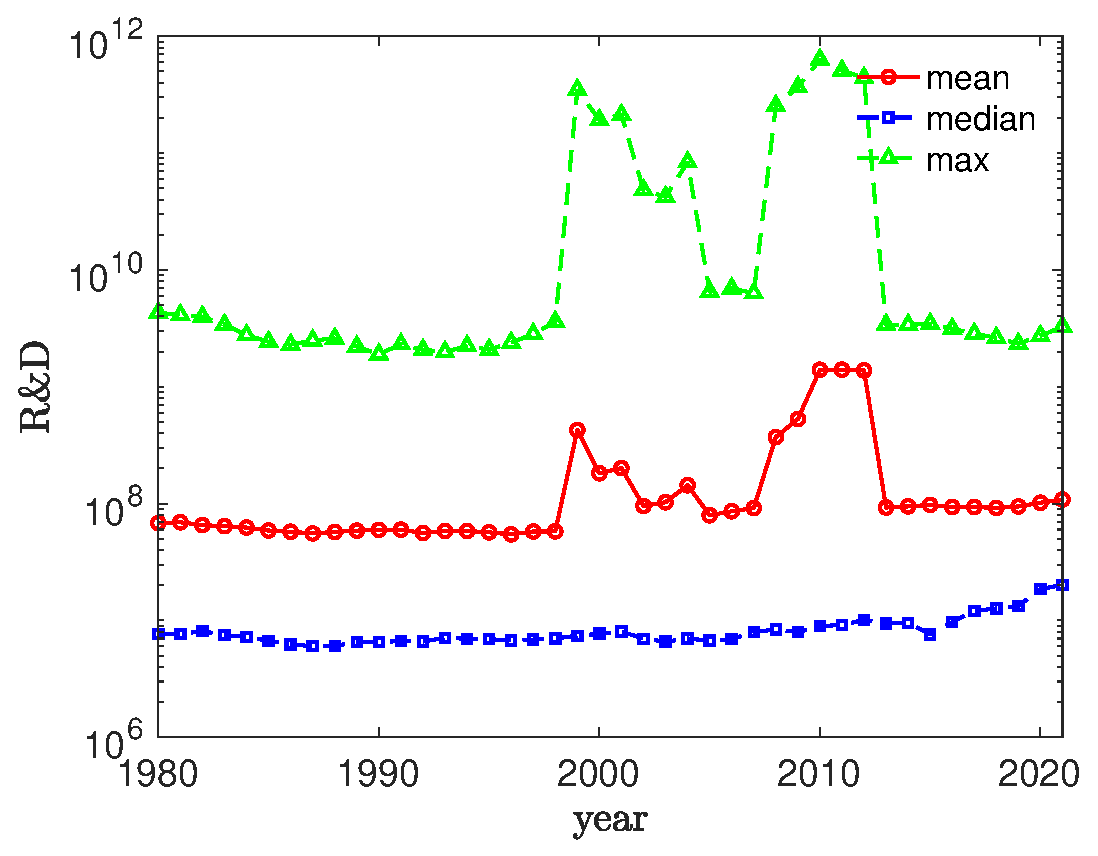
\includegraphics[width=5.25cm,angle=0]{./Figures/compustat_1980_2021_rnd_years_rnd_coll_only.eps}
% \end{minipage}
% \begin{minipage}{0.25\linewidth}
% 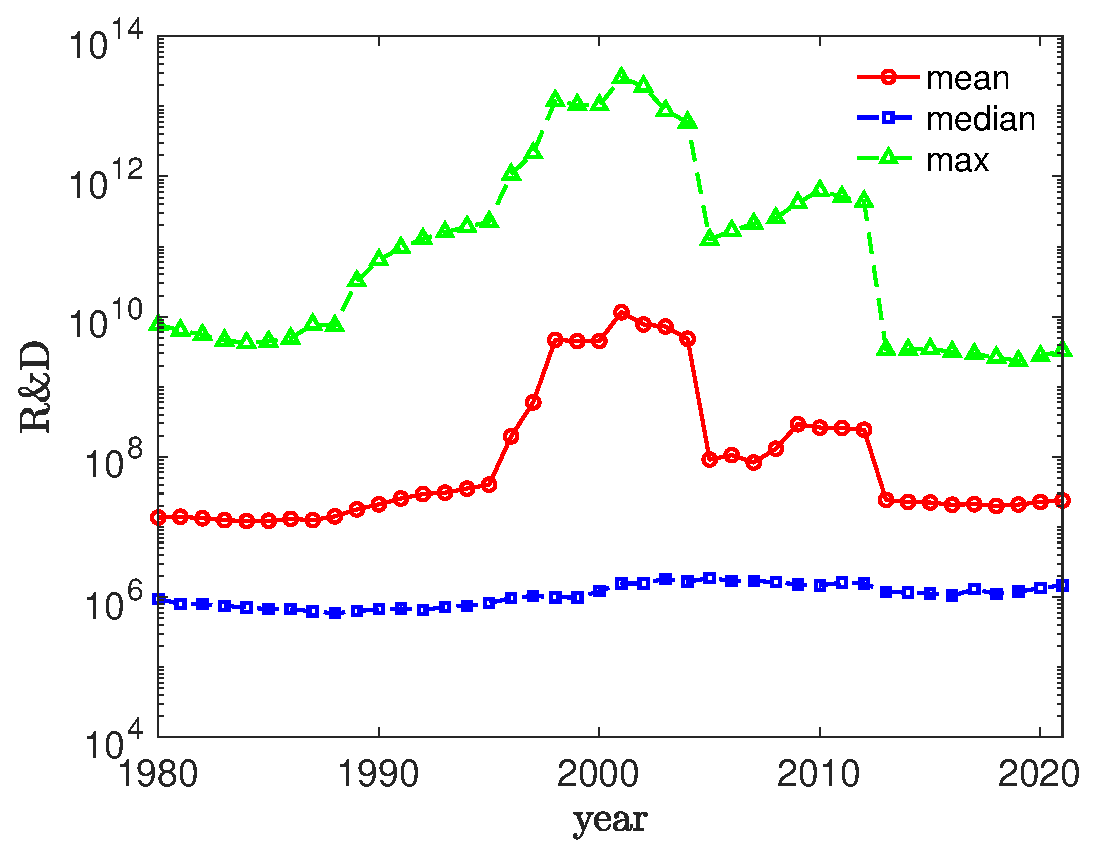
\includegraphics[width=5.25cm,angle=0]{./Figures/compustat_1980_2021_rnd_years_lin_interpol_imputed.eps}
% \end{minipage}
% \caption{The top panels show the time variation (mean, median and maximum) of sales over the years 1980 to 2021, while the bottom panels show the time variation of R\&D expenditures. The panels in the first column show the merged Compustat Fundamentals Annual and Global data. The second column shows the linearly interpolated (over time) and imputed (for missing values) data of the merged Compustat North America Fundamentals Annual and Global databases. The third column shows the corresponding averages only for the firms that participate in R\&D collaborations in the merged Compustat North America Fundamentals Annual and Global data. The last column shows the linearly interpolated (over time) and imputed (for missing values) data for the R\&D collaborating firms in the merged Compustat North America  Fundamentals Annual and Global databases.}
% \label{fig:compustat-time-variation}
% \end{figure}
% \end{landscape}

% \begin{figure}[tbp]
% \begin{minipage}{0.49\linewidth}
% \centering
% %{\small Comp. North Am. \& Glob.}
% 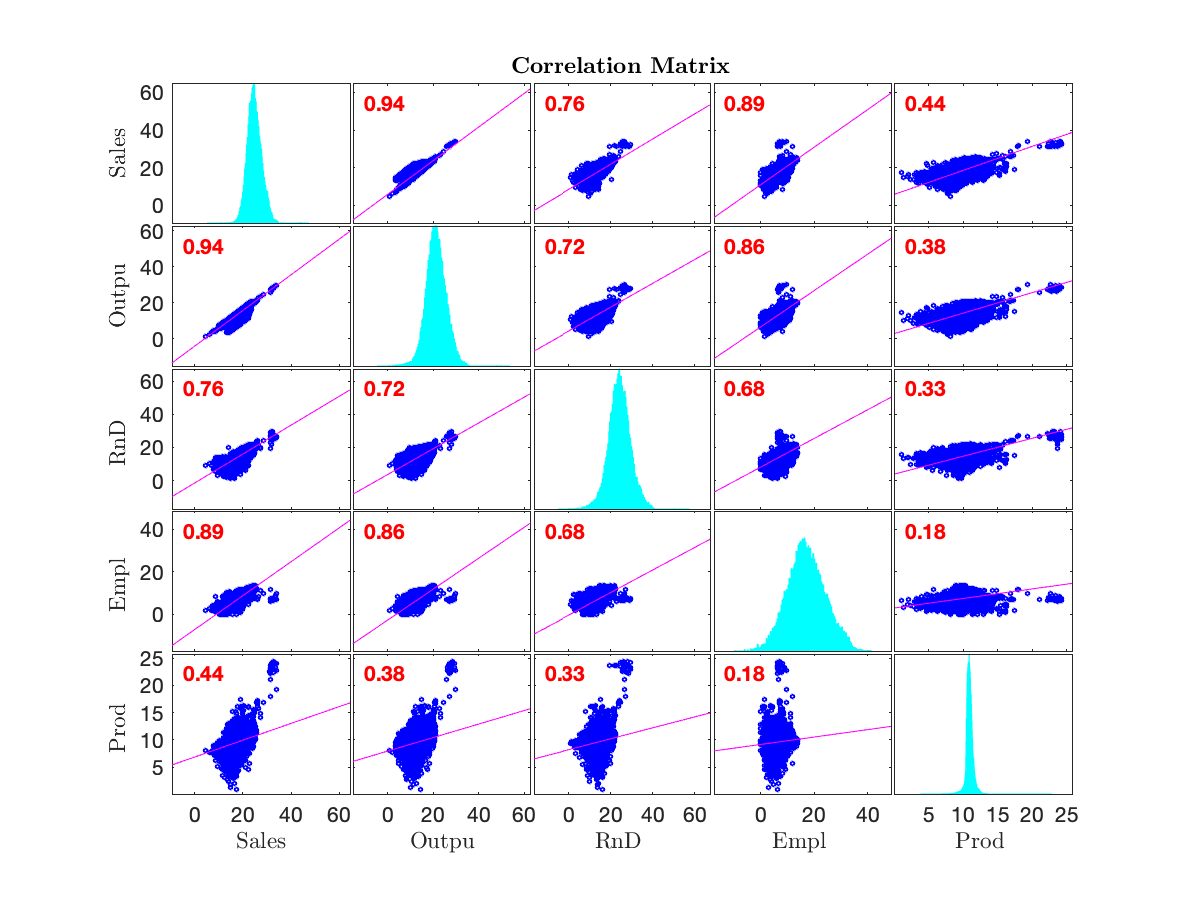
\includegraphics[width=9cm,angle=0]{./Figures/compustat_1980_2021_correlations.eps}
% \end{minipage}
% \begin{minipage}{0.5\linewidth}
% \centering
% %{\small Comp. North Am. \& Glob. (interpol. \& imputed)}
% 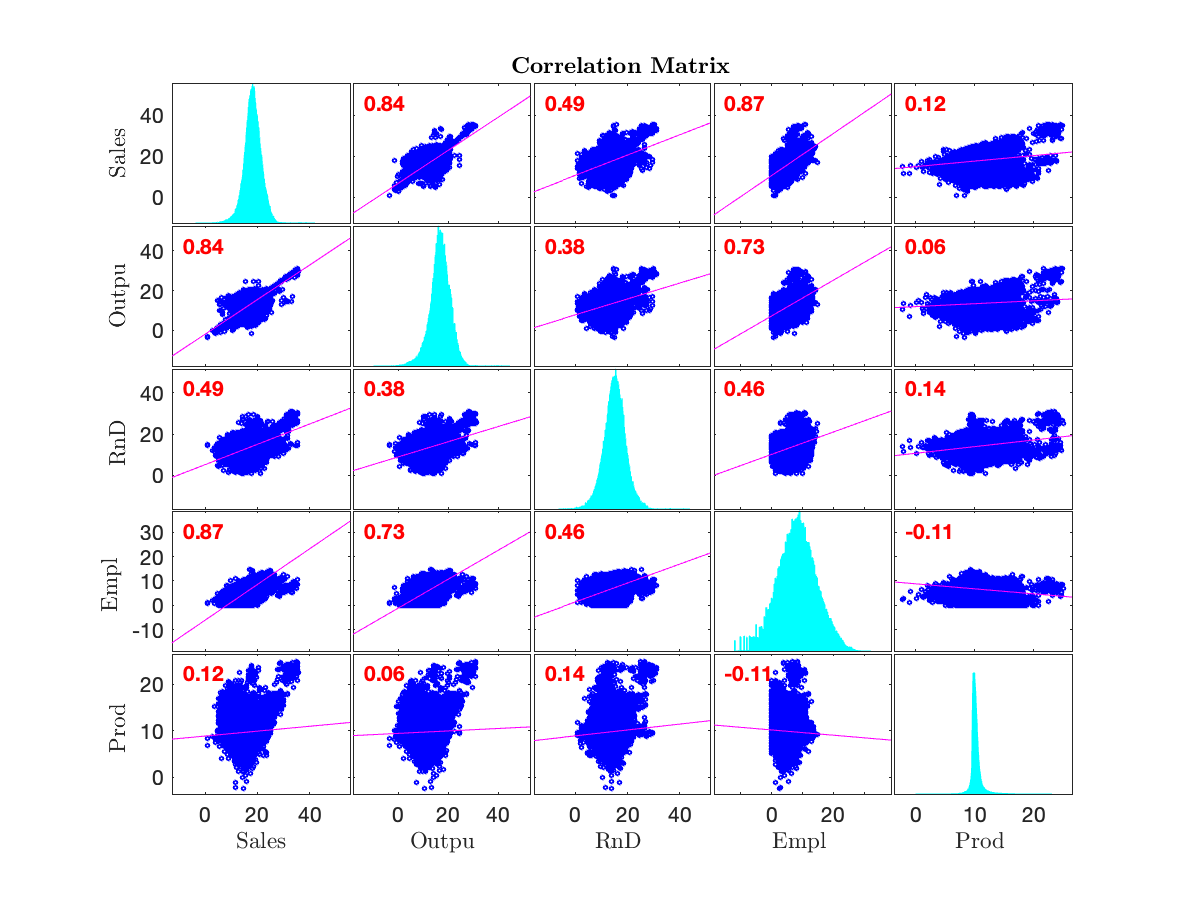
\includegraphics[width=9cm,angle=0]{./Figures/compustat_1980_2021_correlations_lin_interpol_imputed.eps}
% \end{minipage}
% \begin{minipage}{0.49\linewidth}
% \centering
% %{\small R\&D collab. firms only}
% 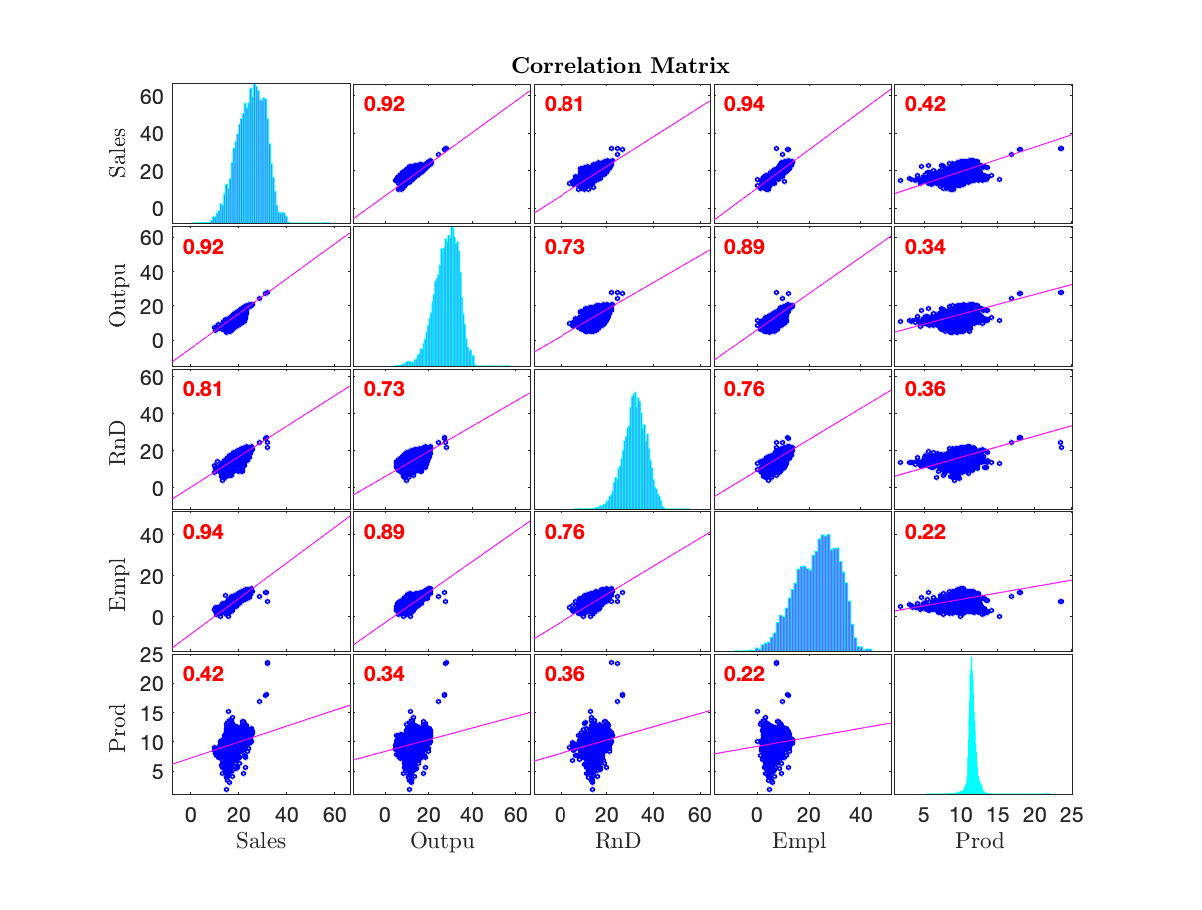
\includegraphics[width=9cm,angle=0]{./Figures/compustat_1980_2021_correlations_rnd_coll_only.eps}
% \end{minipage}
% \begin{minipage}{0.5\linewidth}
% \centering
% %{\small R\&D collab. firms only (interpol. \& imputed)}
% 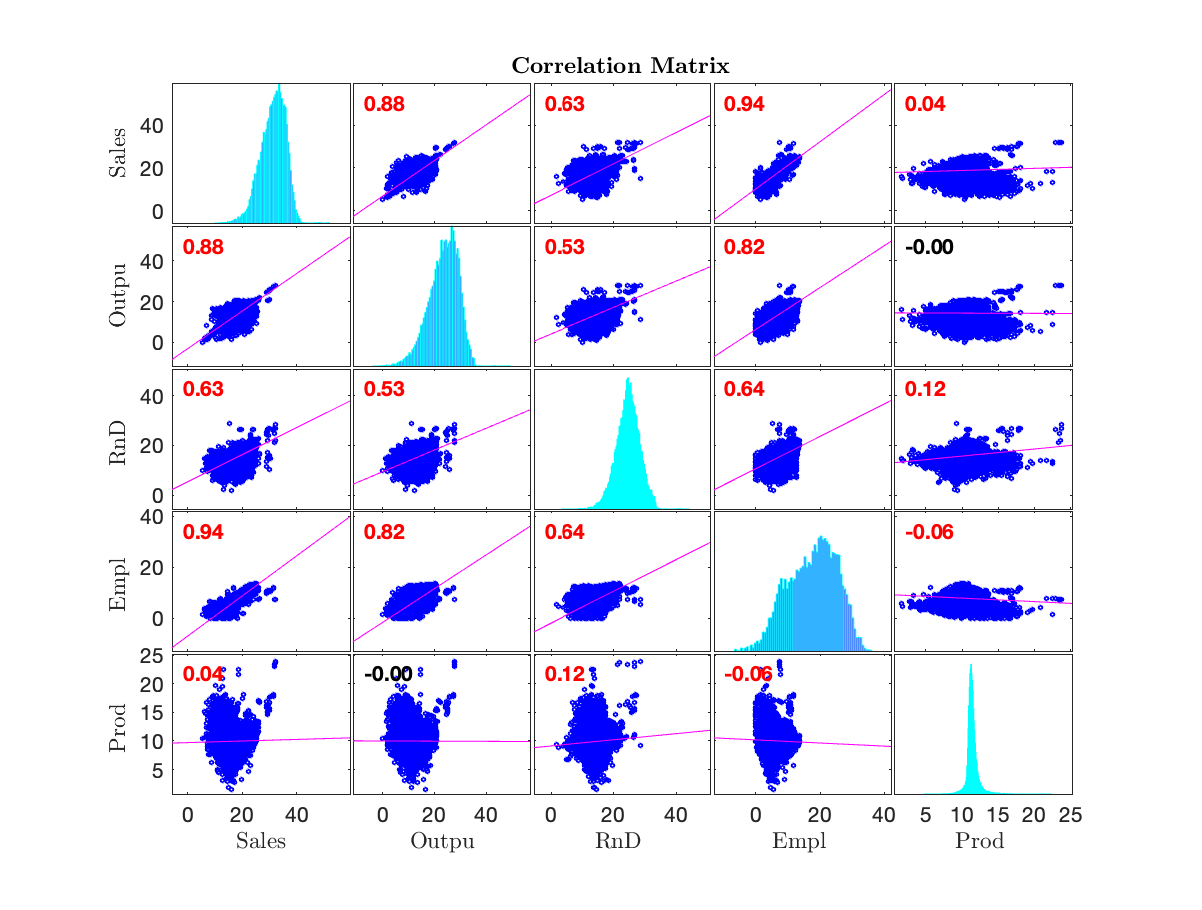
\includegraphics[width=9cm,angle=0]{./Figures/compustat_1980_2021_correlations_lin_interpol_imputed_rnd_coll_only.eps}
% \end{minipage}
% \caption{The top left panel shows the correlation matrix of sales, output, R\&D expenditures, employment and labor productivity (value added divided by the number of employees) for the merged Compustat Fundamentals Annual and Global data pooled across all years. The top right panel shows the corresponding correlation matrix for the linearly interpolated (over time) and imputed (for missing values) data of the merged Compustat North America Fundamentals Annual and Global databases. The bottom left panel shows the correlation matrix for the firms that participate in R\&D collaborations in the merged Compustat North America Fundamentals Annual and Global data. The bottom right panel shows the correlation matrix for the linearly interpolated (over time) and imputed (for missing values) data for the R\&D collaborating firms in the merged Compustat North America  Fundamentals Annual and Global databases.}
% \label{fig:compustat-correlations}
% \end{figure}

% \begin{figure}[tbp]
% \begin{minipage}{0.915\linewidth}
% \centering
% \begin{minipage}{0.24\linewidth}
% \centering
% %{\small a) Comp. North Am. \& Glob.}
% 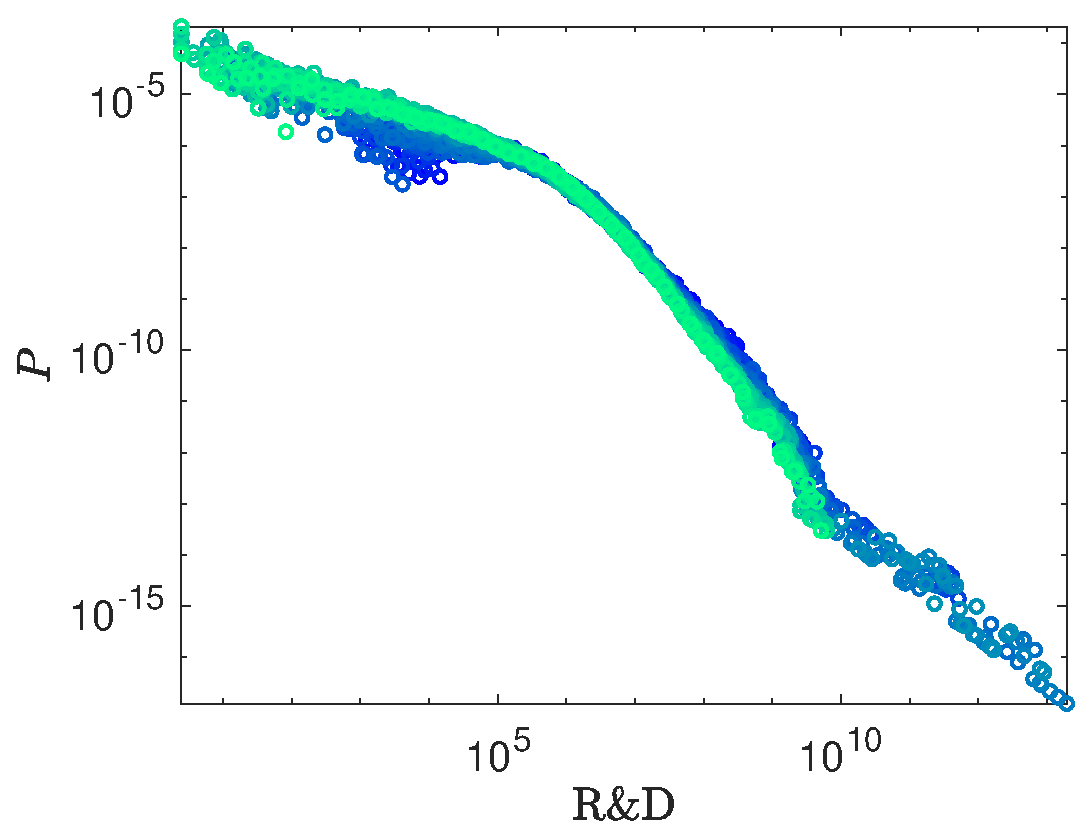
\includegraphics[width=3.75cm,angle=0]{./Figures/compustat_1980_2021_sales_distr.eps}
% \end{minipage}
% \begin{minipage}{0.24\linewidth}
% \centering
% %{\small c) Comp. North Am. \& Glob. (interpol. \& imputed)}
% 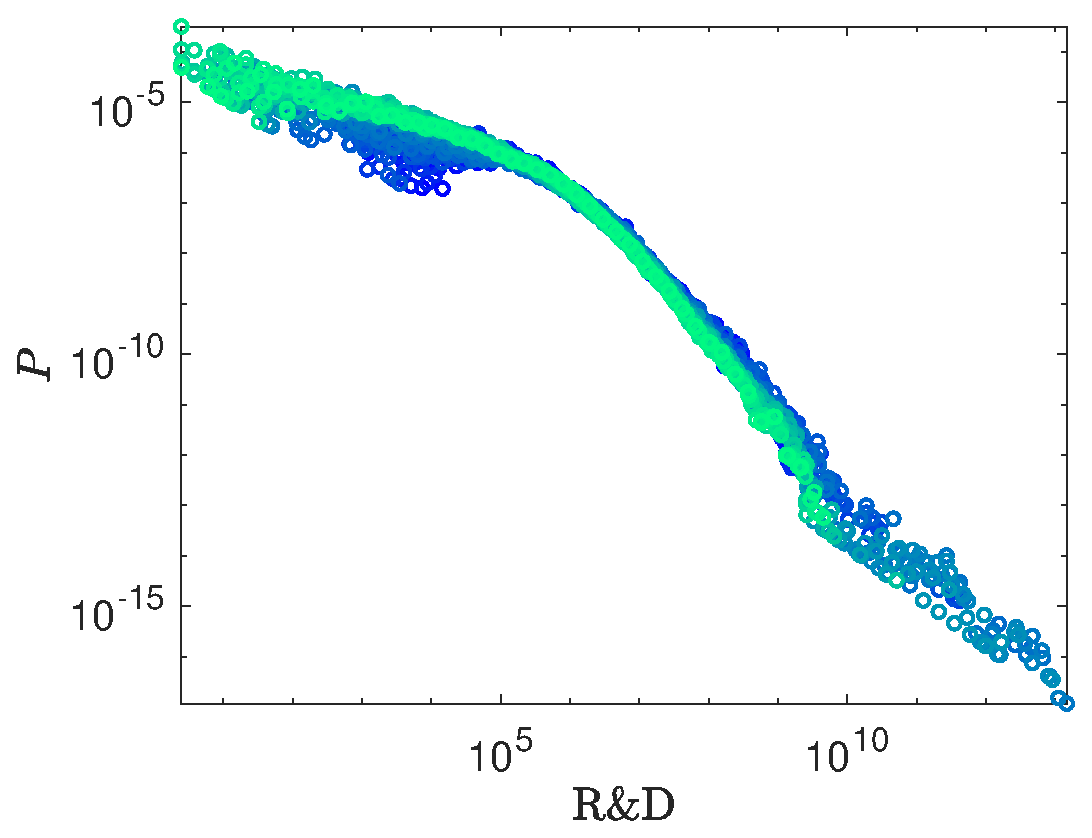
\includegraphics[width=3.75cm,angle=0]{./Figures/compustat_1980_2021_sales_distr_lin_interpol_imputed.eps}
% \end{minipage}
% \begin{minipage}{0.24\linewidth}
% \centering
% %{\small b) R\&D collab. firms only}
% 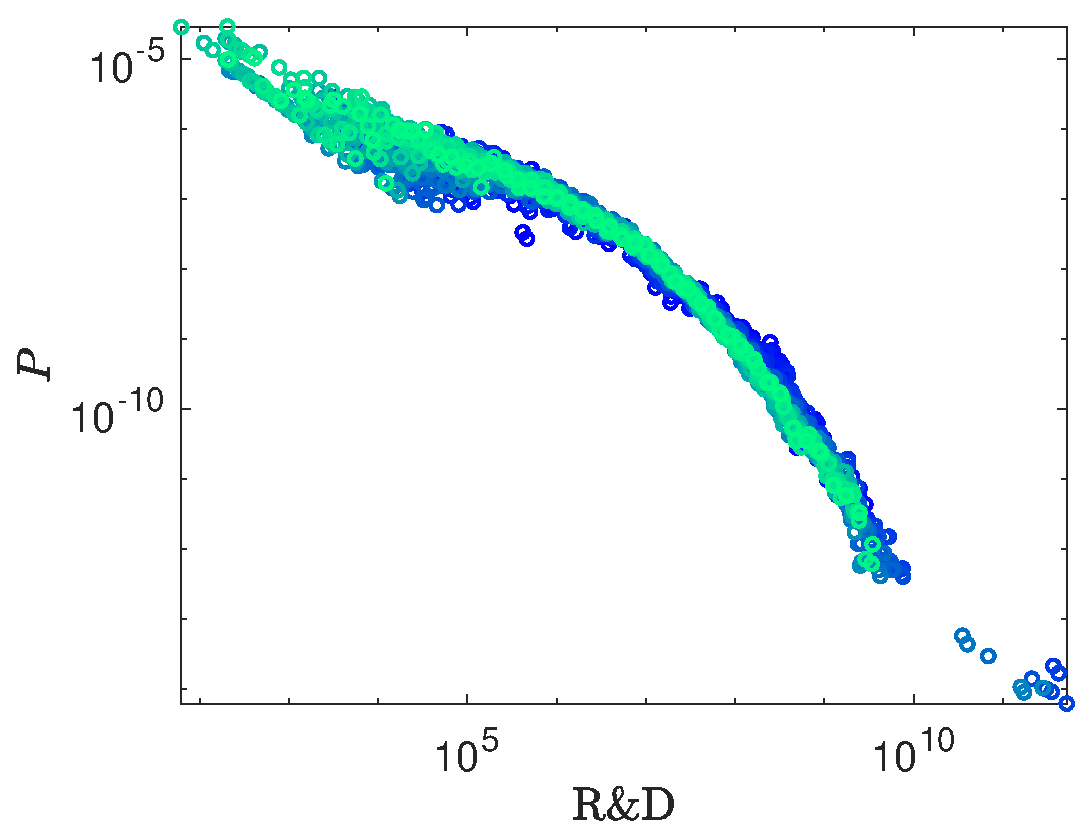
\includegraphics[width=3.75cm,angle=0]{./Figures/compustat_1980_2021_sales_distr_rnd_coll_only.eps}
% \end{minipage}
% \begin{minipage}{0.24\linewidth}
% \centering
% %{\small d) R\&D collab. firms only (interpol. \& imputed)}
% 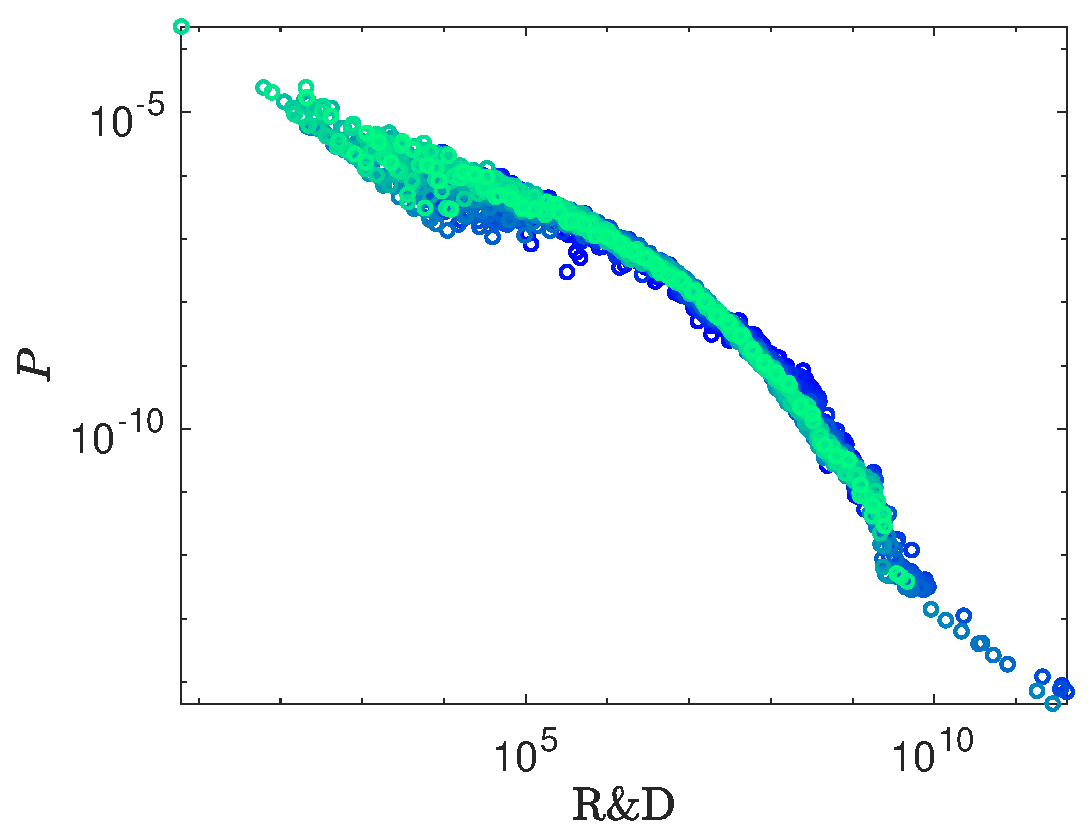
\includegraphics[width=3.75cm,angle=0]{./Figures/compustat_1980_2021_sales_distr_lin_interpol_imputed_rnd_coll_only.eps}
% \end{minipage}
% %
% %
% \begin{minipage}{0.24\linewidth}
% \centering
% 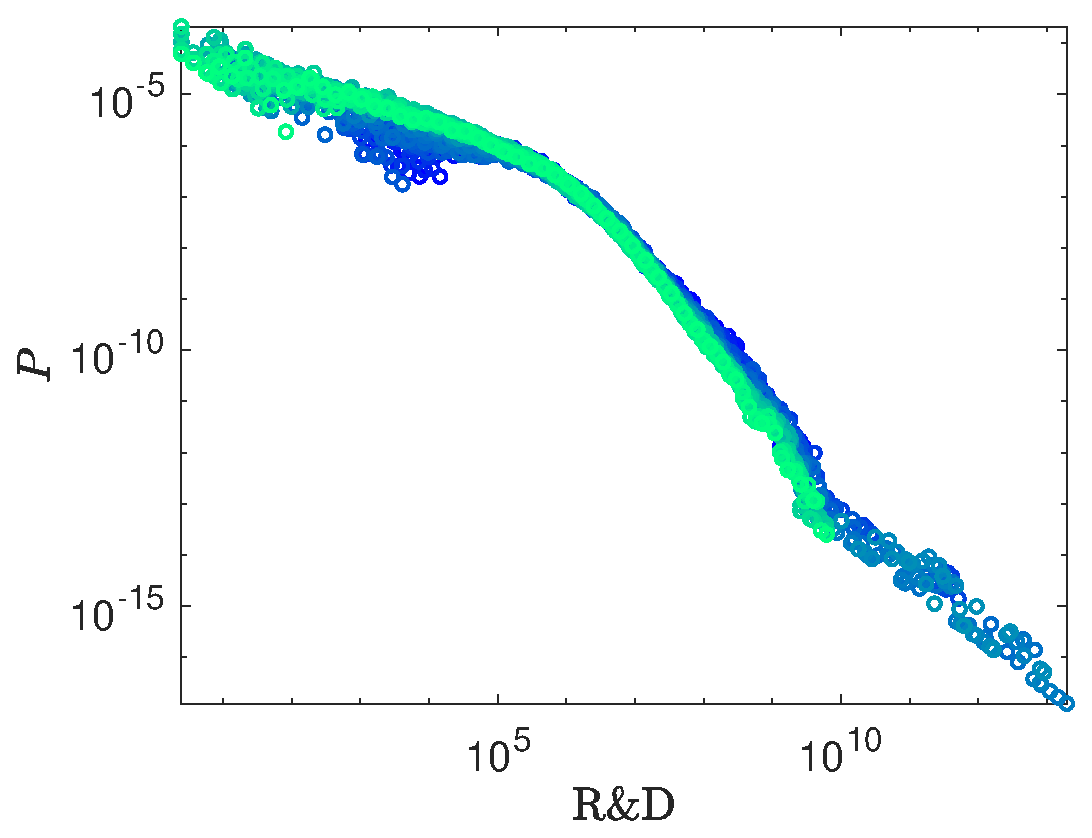
\includegraphics[width=3.75cm,angle=0]{./Figures/compustat_1980_2021_rnd_distr.eps}
% \end{minipage}
% \begin{minipage}{0.24\linewidth}
% 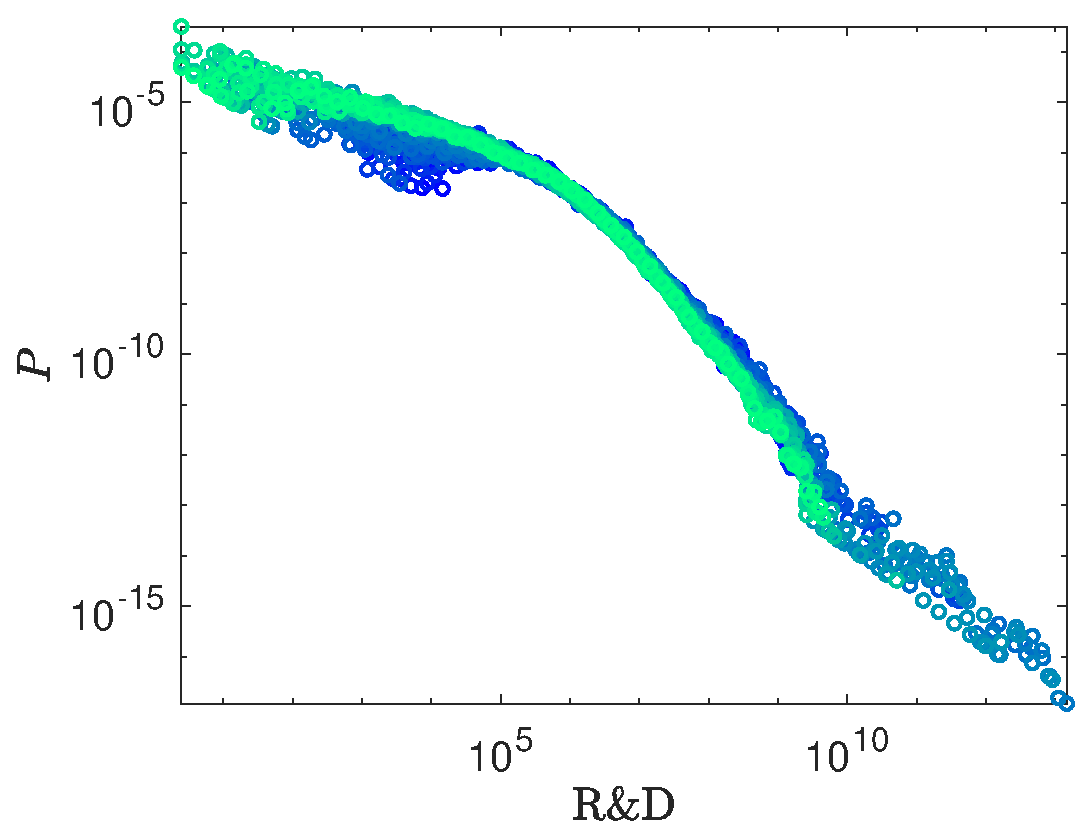
\includegraphics[width=3.75cm,angle=0]{./Figures/compustat_1980_2021_rnd_distr_lin_interpol_imputed.eps}
% \end{minipage}
% \begin{minipage}{0.24\linewidth}
% 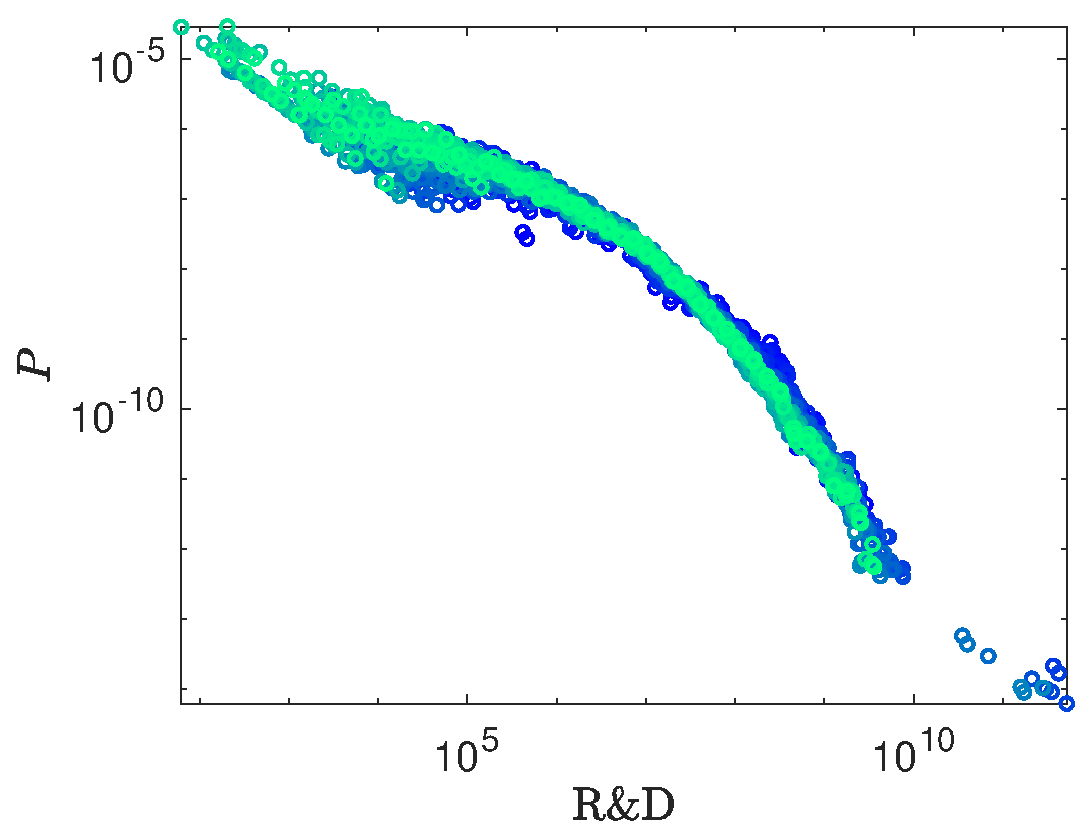
\includegraphics[width=3.75cm,angle=0]{./Figures/compustat_1980_2021_rnd_distr_rnd_coll_only.eps}
% \end{minipage}
% \begin{minipage}{0.24\linewidth}
% 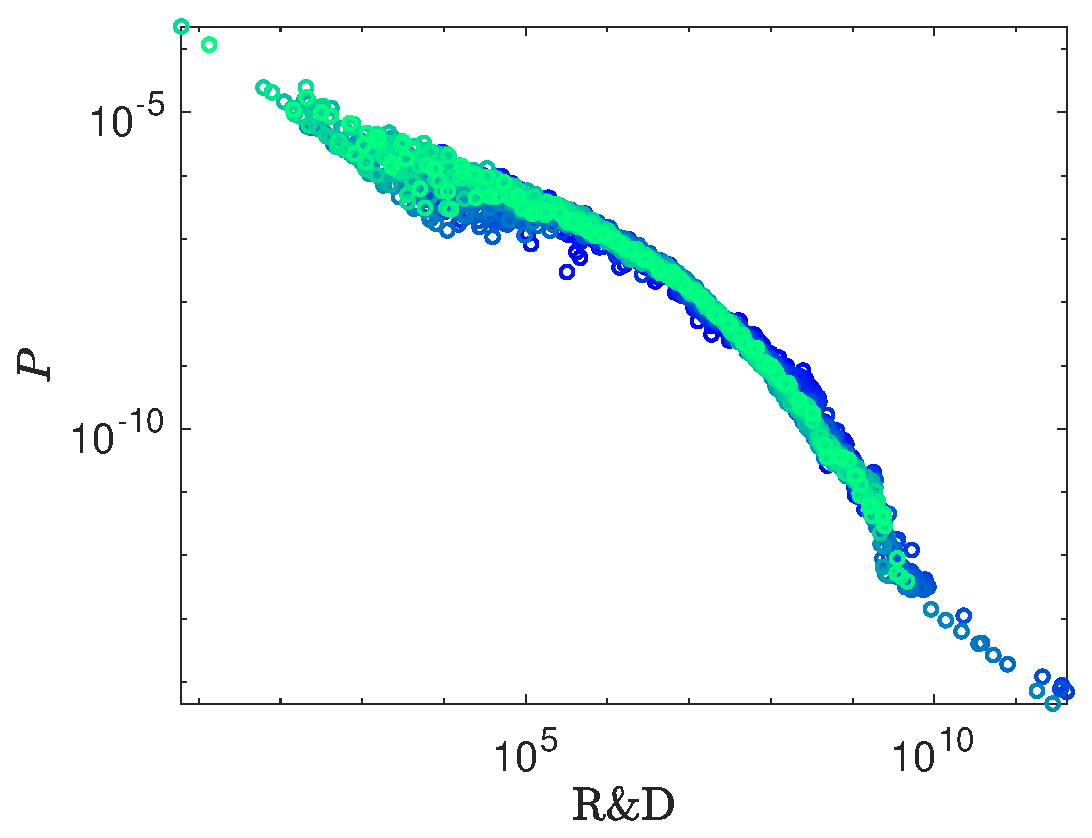
\includegraphics[width=3.75cm,angle=0]{./Figures/compustat_1980_2021_rnd_distr_lin_interpol_imputed_rnd_coll_only.eps}
% \end{minipage}
% %
% %
% \begin{minipage}{0.24\linewidth}
% \centering
% 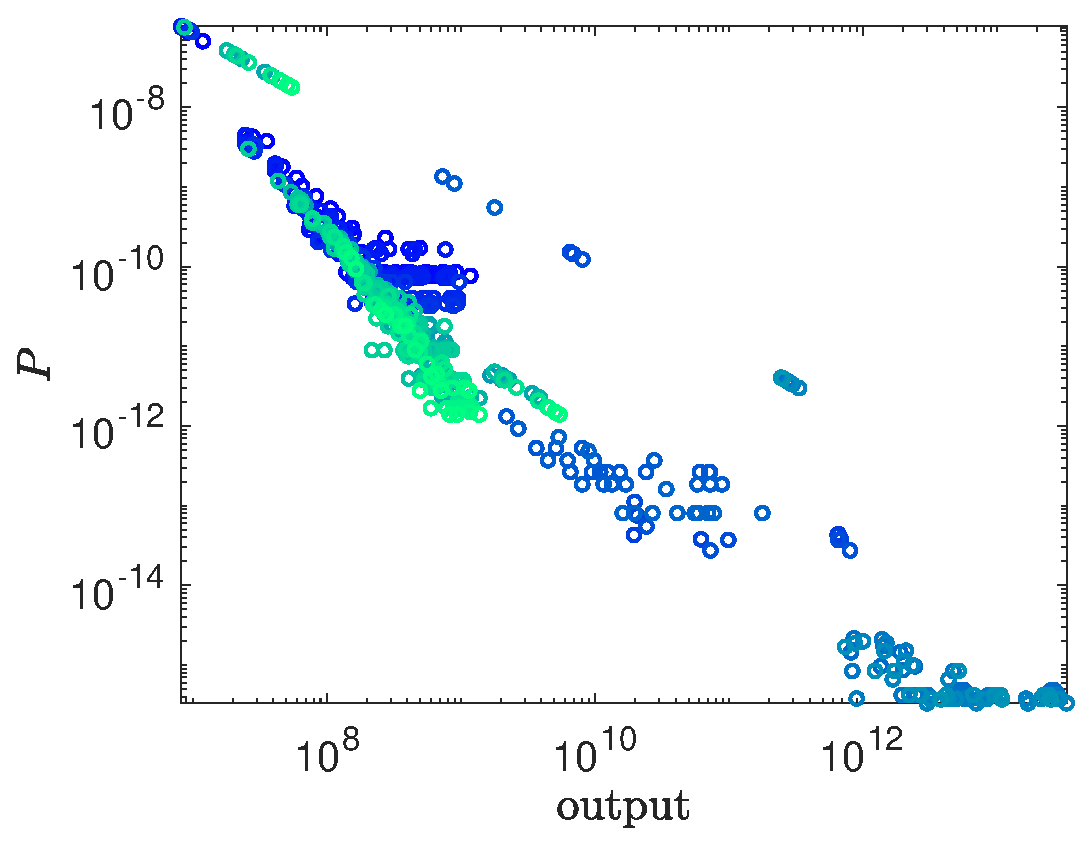
\includegraphics[width=3.75cm,angle=0]{./Figures/compustat_1980_2021_output_distr.eps}
% \end{minipage}
% \begin{minipage}{0.24\linewidth}
% 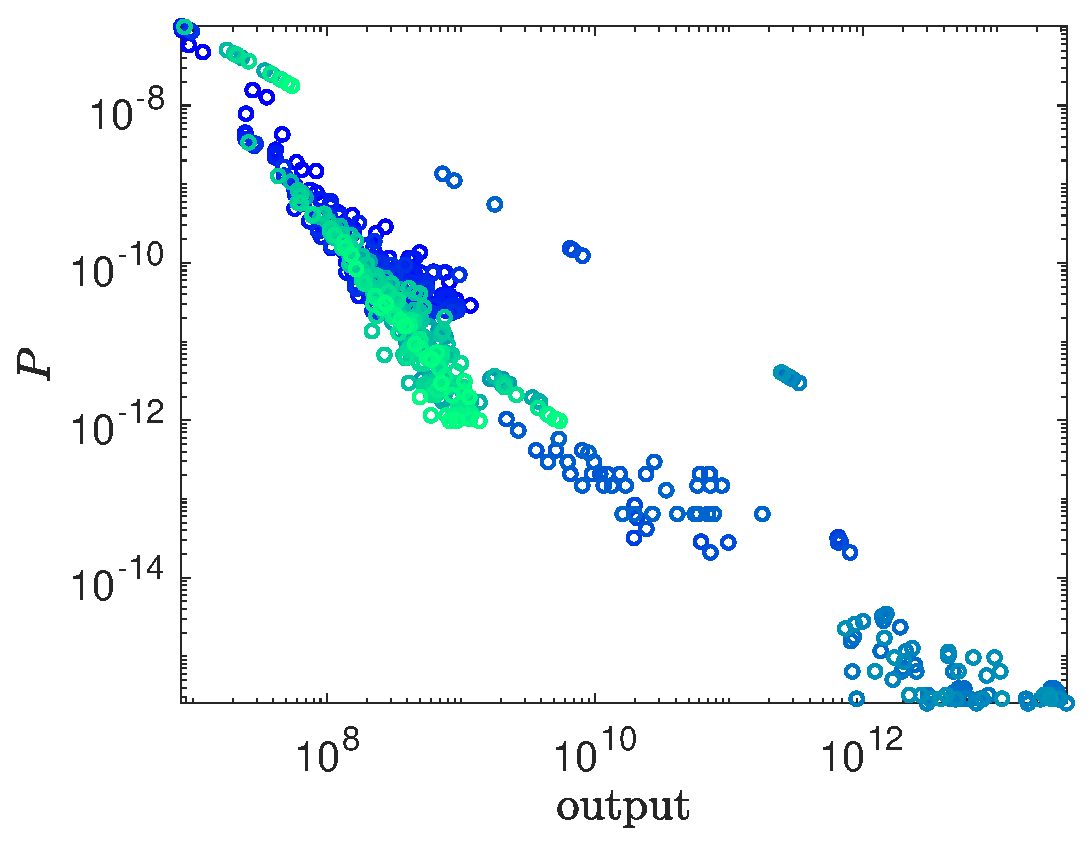
\includegraphics[width=3.75cm,angle=0]{./Figures/compustat_1980_2021_output_distr_lin_interpol_imputed.eps}
% \end{minipage}
% \begin{minipage}{0.24\linewidth}
% 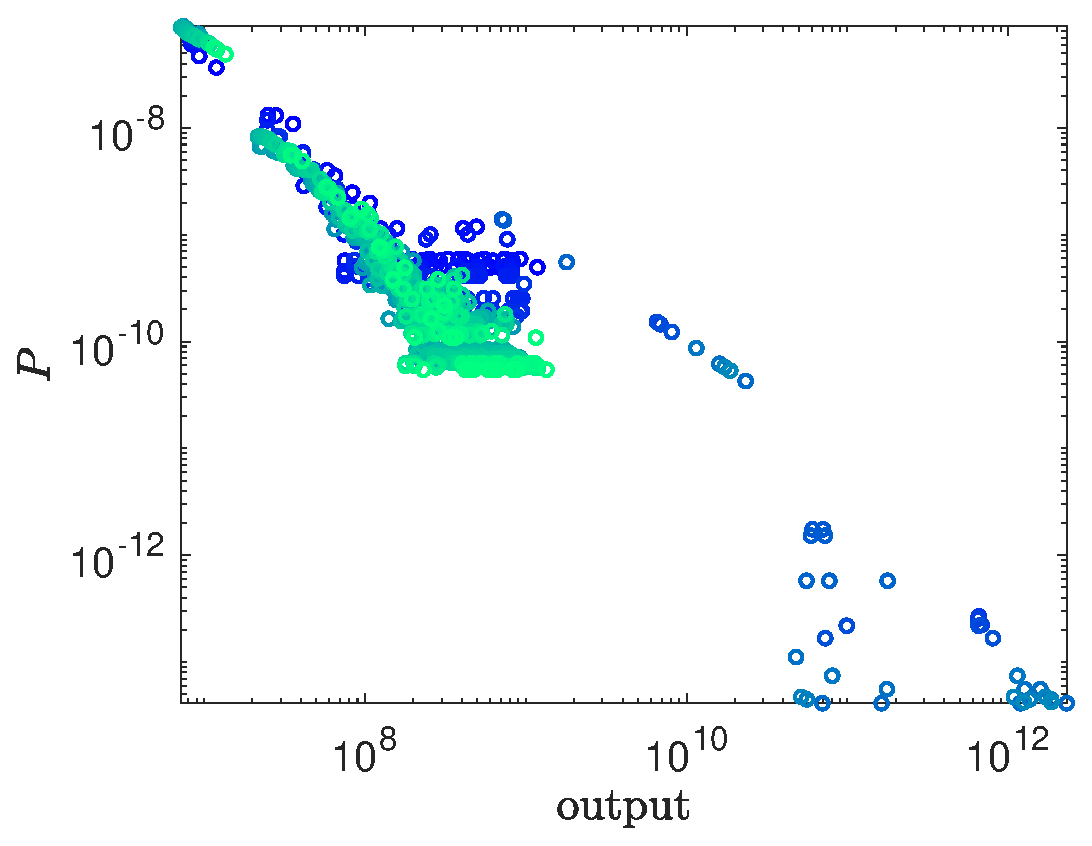
\includegraphics[width=3.75cm,angle=0]{./Figures/compustat_1980_2021_output_distr_rnd_coll_only.eps}
% \end{minipage}
% \begin{minipage}{0.24\linewidth}
% 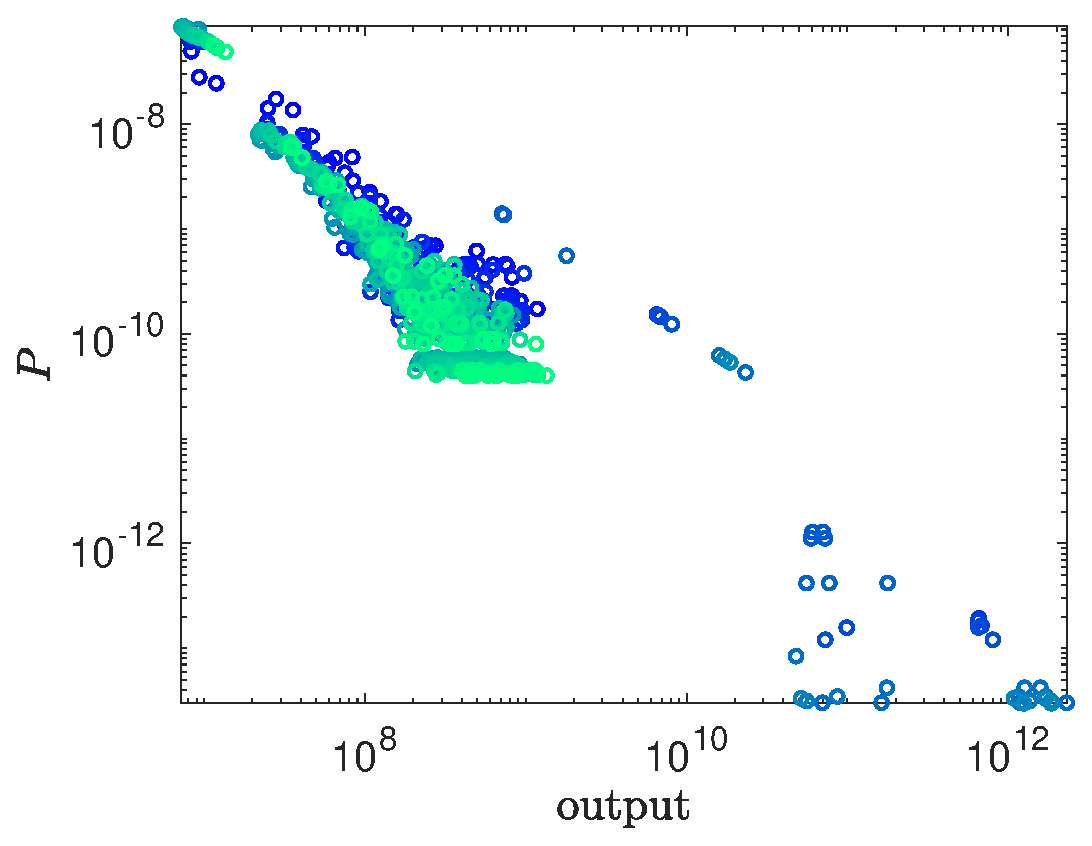
\includegraphics[width=3.75cm,angle=0]{./Figures/compustat_1980_2021_output_distr_lin_interpol_imputed_rnd_coll_only.eps}
% \end{minipage}
% %
% %
% \begin{minipage}{0.24\linewidth}
% \centering
% 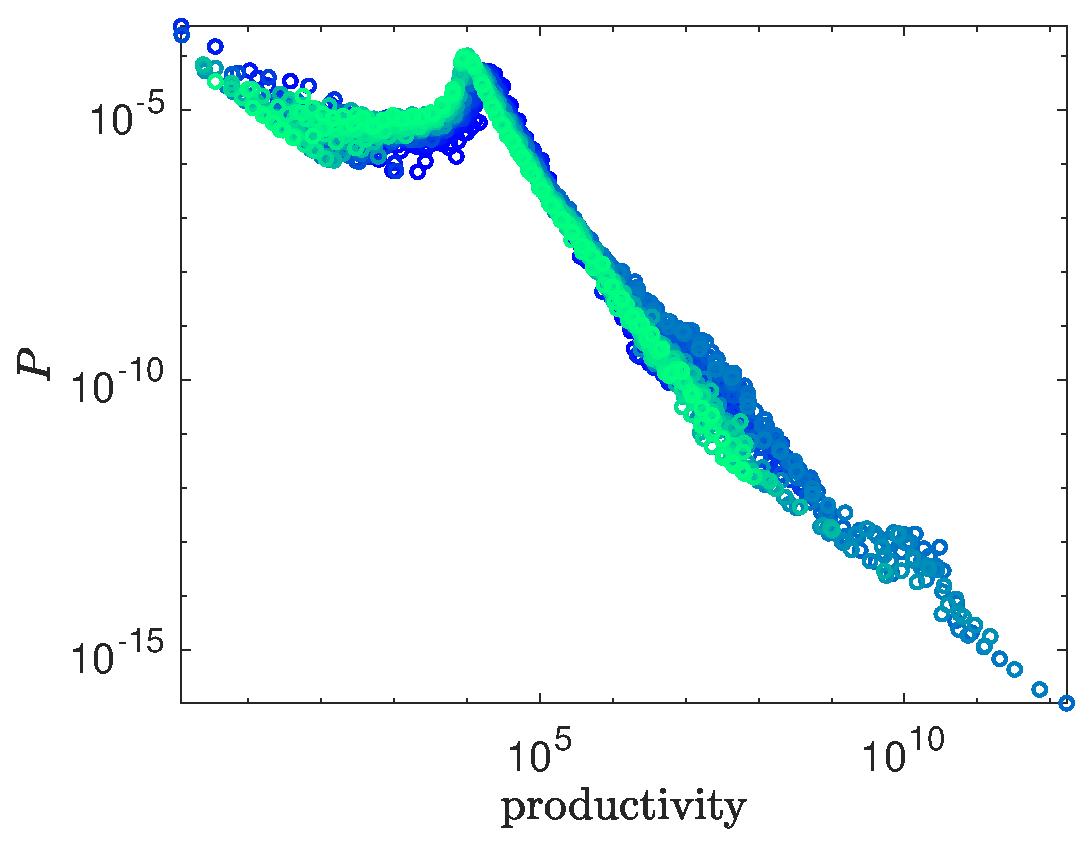
\includegraphics[width=3.75cm,angle=0]{./Figures/compustat_1980_2021_prod_distr.eps}
% \end{minipage}
% \begin{minipage}{0.24\linewidth}
% 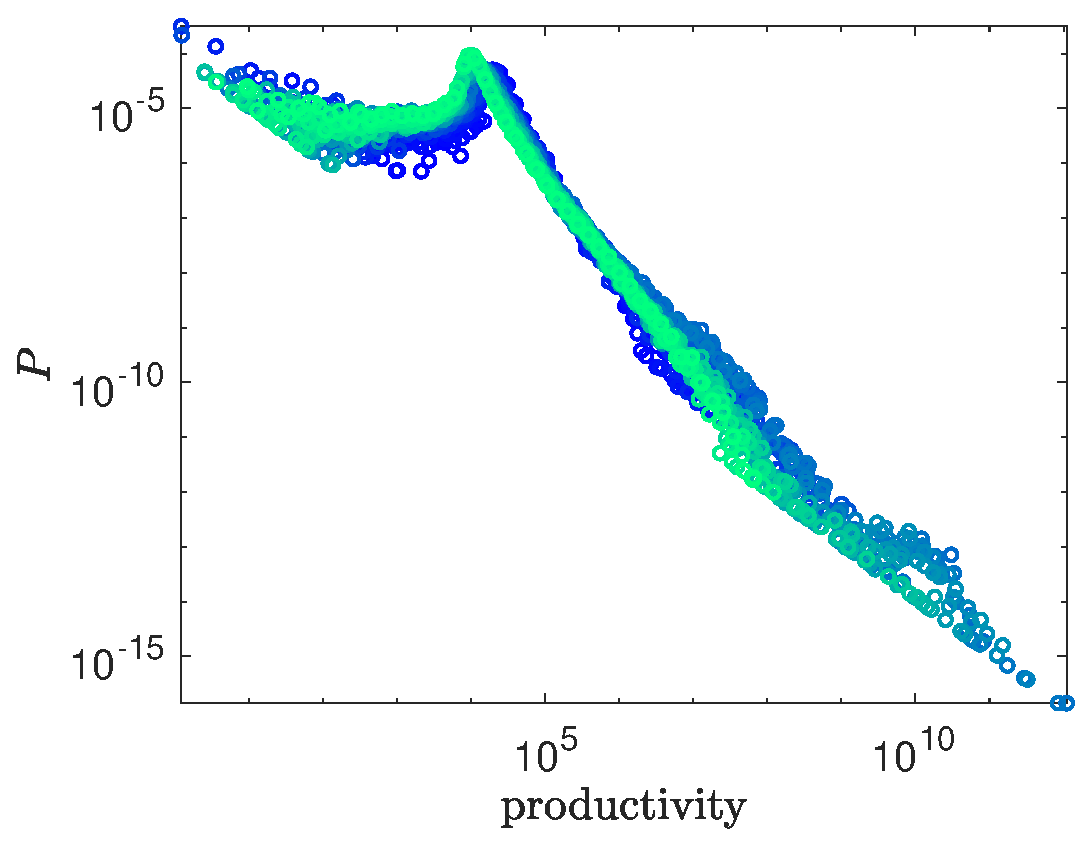
\includegraphics[width=3.75cm,angle=0]{./Figures/compustat_1980_2021_prod_distr_lin_interpol_imputed.eps}
% \end{minipage}
% \begin{minipage}{0.24\linewidth}
% 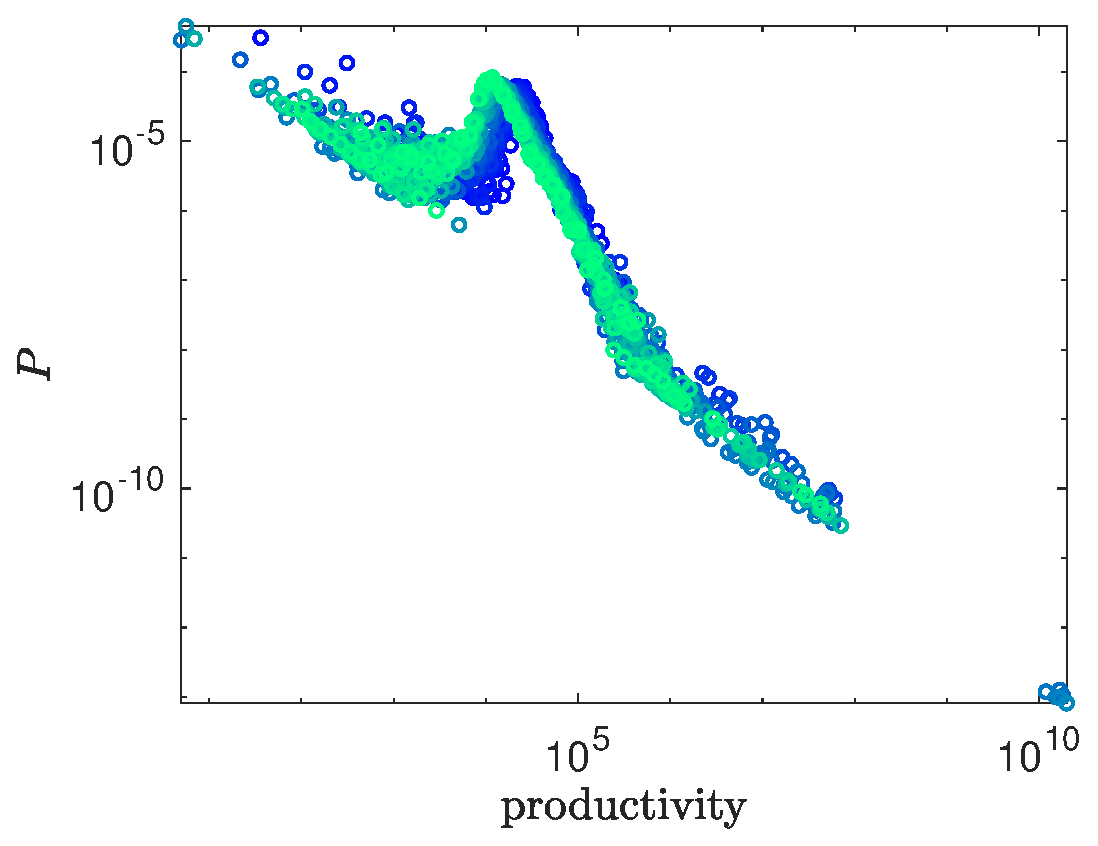
\includegraphics[width=3.75cm,angle=0]{./Figures/compustat_1980_2021_prod_distr_rnd_coll_only.eps}
% \end{minipage}
% \begin{minipage}{0.24\linewidth}
% 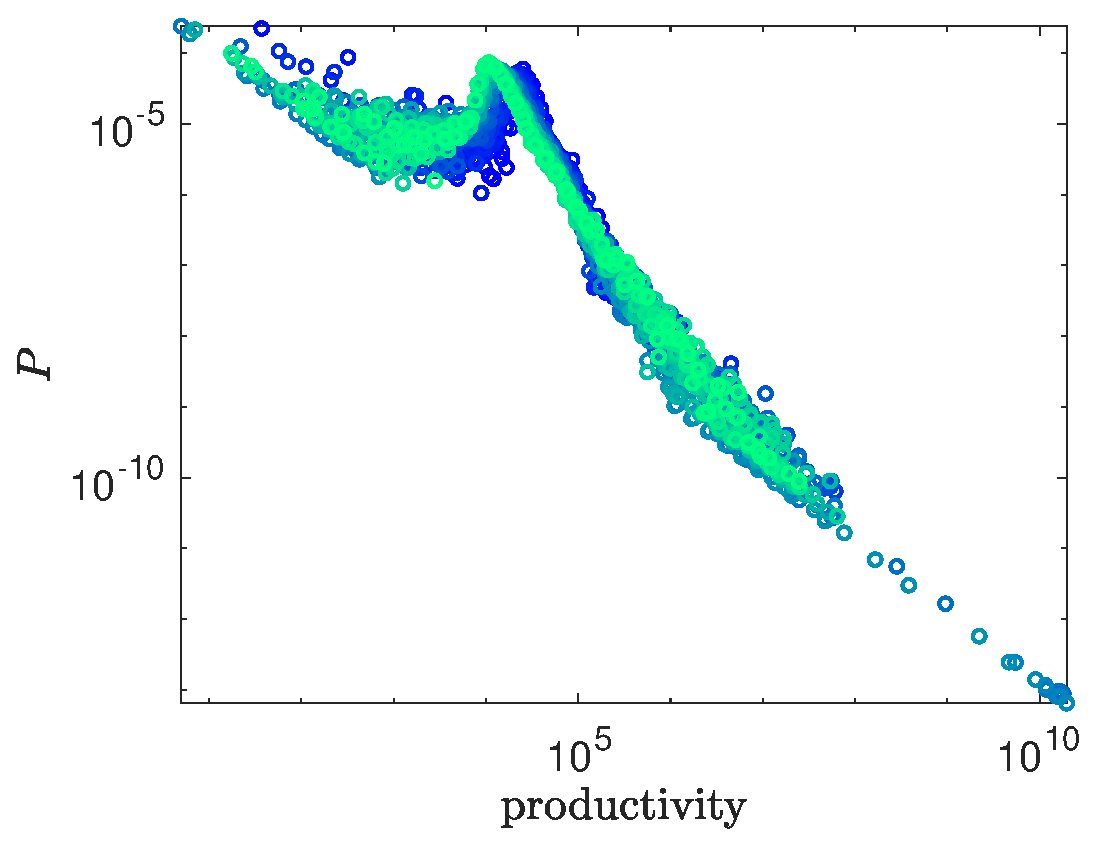
\includegraphics[width=3.75cm,angle=0]{./Figures/compustat_1980_2021_prod_distr_lin_interpol_imputed_rnd_coll_only.eps}
% \end{minipage}
% \end{minipage}
% \hspace{0.5cm}
% \begin{minipage}{0.025\linewidth}
% \vspace{-7.75cm}
% \footnotesize
% \definecolor{col1}{rgb}{0,0,1}
% \definecolor{col2}{rgb}{0,0.032258,0.98387}
% \definecolor{col3}{rgb}{0,0.064516,0.96774}
% \definecolor{col4}{rgb}{0,0.096774,0.95161}
% \definecolor{col5}{rgb}{0,0.12903,0.93548}
% \definecolor{col6}{rgb}{0,0.16129,0.91935}
% \definecolor{col7}{rgb}{0,0.19355,0.90323}
% \definecolor{col8}{rgb}{0,0.22581,0.8871}
% \definecolor{col9}{rgb}{0,0.25806,0.87097}
% \definecolor{col10}{rgb}{0,0.29032,0.85484}
% \definecolor{col11}{rgb}{0,0.32258,0.83871}
% \definecolor{col12}{rgb}{0,0.35484,0.82258}
% \definecolor{col13}{rgb}{0,0.3871,0.80645}
% \definecolor{col14}{rgb}{0,0.41935,0.79032}
% \definecolor{col15}{rgb}{0,0.45161,0.77419}
% \definecolor{col16}{rgb}{0,0.48387,0.75806}
% \definecolor{col17}{rgb}{0,0.51613,0.74194}
% \definecolor{col18}{rgb}{0,0.54839,0.72581}
% \definecolor{col19}{rgb}{0,0.58065,0.70968}
% \definecolor{col20}{rgb}{0,0.6129,0.69355}
% \definecolor{col21}{rgb}{0,0.64516,0.67742}
% \definecolor{col22}{rgb}{0,0.67742,0.66129}
% \definecolor{col23}{rgb}{0,0.70968,0.64516}
% \definecolor{col24}{rgb}{0,0.74194,0.62903}
% \definecolor{col25}{rgb}{0,0.77419,0.6129}
% \definecolor{col26}{rgb}{0,0.80645,0.59677}
% \definecolor{col27}{rgb}{0,0.83871,0.58065}
% \definecolor{col28}{rgb}{0,0.87097,0.56452}
% \definecolor{col29}{rgb}{0,0.90323,0.54839}
% \definecolor{col30}{rgb}{0,0.93548,0.53226}
% \definecolor{col31}{rgb}{0,0.96774,0.51613}
% \definecolor{col32}{rgb}{0,1,0.5}
% \colorbox{col1!50}{1990} \\
% %\colorbox{col2!50}{1991} \\
% %\colorbox{col3!50}{1992} \\
% %\colorbox{col4!50}{1993} \\
% %\colorbox{col5!50}{1994} \\
% \colorbox{col6!50}{1995} \\
% %\colorbox{col7!50}{1996} \\
% %\colorbox{col8!50}{1997} \\
% %\colorbox{col9!50}{1998} \\
% %\colorbox{col10!50}{1999} \\
% \colorbox{col11!50}{2000} \\
% %\colorbox{col12!50}{2001} \\
% %\colorbox{col13!50}{2002} \\
% %\colorbox{col14!50}{2003} \\
% %\colorbox{col15!50}{2004} \\
% \colorbox{col16!50}{2005} \\
% %\colorbox{col17!50}{2006} \\
% %\colorbox{col18!50}{2007} \\
% %\colorbox{col19!50}{2008} \\
% %\colorbox{col20!50}{2009} \\
% \colorbox{col21!50}{2010} \\
% %\colorbox{col22!50}{2011} \\
% %\colorbox{col23!50}{2012} \\
% %\colorbox{col24!50}{2013} \\
% %\colorbox{col25!50}{2014} \\
% \colorbox{col26!50}{2015} \\
% %\colorbox{col27!50}{2016} \\
% %\colorbox{col28!50}{2017} \\
% %\colorbox{col29!50}{2018} \\
% %\colorbox{col30!50}{2019} \\
% \colorbox{col31!50}{2020} \\
% %\colorbox{col32!50}{2021} \\
% \end{minipage}
% \caption{The panels in the top row show the distribution of sales for different years. The panels in the second row the distribution os R\&D expenditures, the third row the distribution of output and the bottom panels the distribution of labor productivity (value added divided by the number of employees). The first column shows the merged Compustat Fundamentals Annual and Global data. The second column shows the linearly interpolated (over time) and imputed (for missing values) data of the merged Compustat North America Fundamentals Annual and Global databases. The third column shows the firms that participate in R\&D collaborations in the merged Compustat North America Fundamentals Annual and Global data. The last column shows the linearly interpolated (over time) and imputed (for missing values) data for the R\&D collaborating firms in the merged Compustat North America  Fundamentals Annual and Global databases.}
% \label{fig:compustat-distr}
% \end{figure}

\FloatBarrier


\end{document}